\documentclass[11pt,A4 paper]{book}
\usepackage[utf8]{inputenc}
\usepackage[colorlinks,linkcolor=blue,hyperfootnotes=false]{hyperref}
\usepackage{graphicx}
\usepackage{multicol}
\usepackage{amsfonts}
\usepackage{amsmath,amssymb,amsthm}
\usepackage{textcomp}
\usepackage{extpfeil}
\usepackage{geometry}
\usepackage{wasysym}
\usepackage{extarrows}
\usepackage[bottom]{footmisc}
\usepackage{enumitem}
\usepackage{textgreek,bm,upgreek,mathrsfs}
\usepackage{stmaryrd}
\usepackage{epigraph}
\usepackage[many]{tcolorbox}
\usepackage[english]{babel}
\usepackage{mathdesign}
\usepackage{setspace}
\usepackage{microtype} 
\usepackage[framemethod=tikz]{mdframed} 
\usepackage[tikz]{bclogo}
\usepackage{lipsum}
\usepackage{ulem}
\usepackage{wrapfig}
\usepackage{color}
\usepackage{epigraph}
\usepackage[many]{tcolorbox}
\usepackage{tikz-cd}
\usepackage{tikz}
\usepackage{showkeys}
\usepackage{fancyhdr}

\usepackage[T1]{fontenc}
\usepackage{palatino}
\linespread{1.05}

\geometry{left=3cm,right=3cm,top=2.5cm,bottom=2.5cm}
\pagestyle{fancy}
\setlength{\headheight}{15.0pt}
\fancyhf{}
\fancyhead[LE,RO]{\thepage}
\fancyhead[RE]{\bf\nouppercase{\rightmark}}
\fancyhead[LO]{\bf\nouppercase{\leftmark}}
\renewcommand{\headrulewidth}{0pt}
\renewcommand{\footrulewidth}{0pt}

\def\sub{\subseteq}
\def\sups{\supseteq}
\def\emp{\varnothing}
\def\GL{\mathrm{GL}}
\def\End{\mathrm{End}}
\def\Hom{\mathrm{Hom}}
\def\Aut{\mathrm{Aut}}
\def\det{\mathrm{det}}
\def\Ext{\mathrm{Ext}}
\def\tr{\mathrm{tr}}
\def\O{\mathrm{O}}
\def\ker{\mathrm{ker}\,}
\def\coker{\mathrm{coker}\,}
\def\im{\mathrm{im}\,}
\def\coim{\mathrm{coim}\,}
\def\rank{\mathrm{rank}\,}
\def\char{\mathrm{char}\,}
\def\supp{\mathrm{supp}\,}
\def\sign{\mathrm{sign}}
\def\Int{\mathrm{Int}}
\def\id{\mathrm{id}}
\def\pr{\mathrm{pr}\,}
\def\St{\mathrm{St}\,}
\def\st{\mathrm{st}\,}
\def\C{\mathbb{C}}
\def\K{\mathbb{K}}
\def\F{\mathbb{F}}
\def\R{\mathbb{R}}
\def\B{\mathbb{B}}
\def\Q{\mathbb{Q}}
\def\Z{\mathbb{Z}}
\def\N{\mathbb{N}}
\def\T{\mathbb{T}}
\def\H{\mathbb{H}}
\def\RP{\mathbb{R}\mathrm{P}}
\def\CP{\mathbb{C}\mathrm{P}}
\def\P{\mathbb{P}}
\def\eps{\varepsilon}
\def\And{\quad\textit{and}\quad}
\def\for{\quad\textit{for}\quad}
\makeatletter
\@addtoreset{equation}{section}
\makeatother
\renewcommand{\theequation}{\arabic{section}.\arabic{equation}}

\makeatletter
\newcommand{\rmnum}[1]{\romannumeral #1}
\newcommand{\Rmnum}[1]{\expandafter\@slowromancap\romannumeral #1@}
\makeatletter
\let\save@mathaccent\mathaccent
\newcommand*\if@single[3]{%
	\setbox0\hbox{${\mathaccent"0362{#1}}^H$}%
	\setbox2\hbox{${\mathaccent"0362{\kern0pt#1}}^H$}%
	\ifdim\ht0=\ht2 #3\else #2\fi
}
%The bar will be moved to the right by a half of \macc@kerna, which is computed by amsmath:
\newcommand*\rel@kern[1]{\kern#1\dimexpr\macc@kerna}
%If there's a superscript following the bar, then no negative kern may follow the bar;
%an additional {} makes sure that the superscript is high enough in this case:
\newcommand*\widebar[1]{\@ifnextchar^{{\wide@bar{#1}{0}}}{\wide@bar{#1}{1}}}
%Use a separate algorithm for single symbols:
\newcommand*\wide@bar[2]{\if@single{#1}{\wide@bar@{#1}{#2}{1}}{\wide@bar@{#1}{#2}{2}}}
\newcommand*\wide@bar@[3]{%
	\begingroup
	\def\mathaccent##1##2{%
		%Enable nesting of accents:
		\let\mathaccent\save@mathaccent
		%If there's more than a single symbol, use the first character instead (see below):
		\if#32 \let\macc@nucleus\first@char \fi
		%Determine the italic correction:
		\setbox\z@\hbox{$\macc@style{\macc@nucleus}_{}$}%
		\setbox\tw@\hbox{$\macc@style{\macc@nucleus}{}_{}$}%
		\dimen@\wd\tw@
		\advance\dimen@-\wd\z@
		%Now \dimen@ is the italic correction of the symbol.
		\divide\dimen@ 3
		\@tempdima\wd\tw@
		\advance\@tempdima-\scriptspace
		%Now \@tempdima is the width of the symbol.
		\divide\@tempdima 10
		\advance\dimen@-\@tempdima
		%Now \dimen@ = (italic correction / 3) - (Breite / 10)
		\ifdim\dimen@>\z@ \dimen@0pt\fi
		%The bar will be shortened in the case \dimen@<0 !
		\rel@kern{0.6}\kern-\dimen@
		\if#31
		\overline{\rel@kern{-0.6}\kern\dimen@\macc@nucleus\rel@kern{0.4}\kern\dimen@}%
		\advance\dimen@0.4\dimexpr\macc@kerna
		%Place the combined final kern (-\dimen@) if it is >0 or if a superscript follows:
		\let\final@kern#2%
		\ifdim\dimen@<\z@ \let\final@kern1\fi
		\if\final@kern1 \kern-\dimen@\fi
		\else
		\overline{\rel@kern{-0.6}\kern\dimen@#1}%
		\fi
	}%
	\macc@depth\@ne
	\let\math@bgroup\@empty \let\math@egroup\macc@set@skewchar
	\mathsurround\z@ \frozen@everymath{\mathgroup\macc@group\relax}%
	\macc@set@skewchar\relax
	\let\mathaccentV\macc@nested@a
	%The following initialises \macc@kerna and calls \mathaccent:
	\if#31
	\macc@nested@a\relax111{#1}%
	\else
	%If the argument consists of more than one symbol, and if the first token is
	%a letter, use that letter for the computations:
	\def\gobble@till@marker##1\endmarker{}%
	\futurelet\first@char\gobble@till@marker#1\endmarker
	\ifcat\noexpand\first@char A\else
	\def\first@char{}%
	\fi
	\macc@nested@a\relax111{\first@char}%
	\fi
	\endgroup
}
\makeatother
\renewcommand{\thefigure}{\arabic{chapter}.\arabic{figure}}
\renewcommand{\theequation}{\arabic{section}.\arabic{equation}}
\makeatletter

\makeatletter
\newcommand{\colim@}[2]{%
	\vtop{\m@th\ialign{##\cr
			\hfil$#1\operator@font colim$\hfil\cr
			\noalign{\nointerlineskip\kern1.5\ex@}#2\cr
			\noalign{\nointerlineskip\kern-\ex@}\cr}}%
}
\renewcommand{\varprojlim}{%
	\mathop{\mathpalette\varlim@{\leftarrowfill@\scriptscriptstyle}}\nmlimits@
}
\renewcommand{\varinjlim}{%
	\mathop{\mathpalette\varlim@{\rightarrowfill@\scriptscriptstyle}}\nmlimits@
}
\makeatother

\def\llim{\varprojlim\limits}
\def\rlim{\varinjlim\limits}
\newtheorem{remark}{Remark}[section]
\newtheorem{theorem}{Theorem}[section]
\newtheorem{lemma}[theorem]{Lemma}
\newtheorem{corollary}[theorem]{Corollary}
\newtheorem{proposition}[theorem]{Proposition}
\newtheorem{definition}[theorem]{Definition}
\theoremstyle{definition}
\newtheorem{exercise}{Exercise}[section]
\newtheorem{example}[theorem]{Example}

\makeatother
\title{Algebraic Topology}
\begin{document}
\maketitle
\tableofcontents
\setlength\abovedisplayskip{3pt}
\setlength\belowdisplayskip{3pt}

\iffalse
\chapter{Topology}
\section{Continuity}
\begin{definition}
Let $X$ be a metric space. A function $f : X \to\R$ is called \textbf{lower continuous} at $a\in X$ if,
for each sequence $(x_n)$ in $X$ such that $\lim x_n=a$, we have $f(a)\leq\varliminf f(x_n)$. It is called upper continuous at $a$ if $-f$ is lower continuous at $a$, that is, $f(a)\geq\varlimsup f(x_n)$. Finally $f$ is called lower continuous (or upper continuous) if $f$ is lower continuous (or upper continuous) at each point of $X$.\\
\end{definition}
\begin{proposition}\label{lower continuous open closed iff}
Let $f:X\to\R$ be a function where $X$ is a metric space.
\begin{itemize}
\item[$(a)$] Show the  equivalence of the following:
\begin{itemize}
\item[$(\rmnum{1})$] $f$ is lower continuous.
\item[$(\rmnum{2})$] For each $a\in X$ and $\varepsilon>0$, there is some $U\in\mathcal{U}(a)$ such that $f(x) > f(a)-\varepsilon$ for all $x\in U$.
\item[$(\rmnum{3})$] For each $\alpha\in\mathbb{R}$, $f^{-1}((\alpha,\infty))$ is open.
\item[$(\rmnum{4})$] For each $\alpha\in\mathbb{R}$, $f^{-1}((-\infty,\alpha])$ is closed.
\end{itemize}
\item[$(b)$] $f$ is continuous if and only if $f$ is lower and upper continuous.
\item[$(c)$] Let $\chi_A$ be the characteristic function of $A\sub X$. Then $A$ is open if and only if $\chi_A$ is lower continuous.
\item[$(d)$] Let $X$ be compact and $f : X\to\mathbb{R}$ lower continuous. Then $f$ attains its minimum, that is, there is some $x\in X$ such that $f(x)\leq f(y)$ for all $y\in X$.
\end{itemize}
\end{proposition}
\begin{proof}This definition can be treated as a generazation of continuity.
\begin{itemize}
\item[$(a)$]
$(\rmnum{1})\Rightarrow(\rmnum{2})$: Let $f$ be lower continuous, and choose $a\in X$. From the definitin we know that $f(a)\leq\varliminf f(x_n)$ for any sequnce $(x_n)$ in $X$ such that $\lim_nx_n=a$. Now we suppose that there is no $U\in\mathcal{U}(a)$ with the desired property, then there exists an $\varepsilon_0$ such that for any $n\in\mathbb{N}$ we can find $x_n\in\mathbb{B}(a,\frac{1}{n})$ with $f(x_n)\leq f(a)-\varepsilon_0$. In particular, $\lim_nx_n=a$ and we have $\varliminf f(x_n)\leq f(a)-\varepsilon_0$, which is a contradiction.\par
$(\rmnum{2})\Rightarrow(\rmnum{3})$: Now if $x_0\in f^{-1}((\alpha,\infty))$, then we have $f(x_0)>\alpha$ and there is $U\in\mathcal{U}(x_0)$ such that $f(x)>f(x_0)-\frac{f(x_0)-\alpha}{2}>\alpha$ for all $x\in U$, hence $U\sub f^{-1}((\alpha,\infty))$. And by the definition $f^{-1}((\alpha,\infty))$ is open.\par
$(\rmnum{3})\Rightarrow(\rmnum{4})$: This is just from
\[\mathbb{R}-f^{-1}((\alpha,\infty))=f^{-1}(\mathbb{R}-(\alpha,\infty))=f^{-1}((-\infty,\alpha])\]
$(\rmnum{4})\Rightarrow(\rmnum{1})$: 
Now suppose for each $\alpha\in\mathbb{R}$, $f^{-1}((\alpha,\infty))$ is open, then for $f(a)$, we have $U\sub f^{-1}((\alpha,\infty))$ such that $f(x)\geq f(a)$ for $x\in U$. Now for a sequence $(x_n)$ with $\lim x_n=a$, there is $N$ such that $x_n\in U$ for $n>N$, and hence $f(x_n)\geq f(a)$ for $n>N$. This yields $\varliminf f(x_n)\geq f(a)$, so $f$ is lower continuous.
\item[$(b)$] If $f$ is continuous then it is clearly lower and upper continuous since we have $f(x_n)=f(a)$. And if $f$ is lower and upper continuous, we have $\varlimsup f(x_n)\leq f(a)\leq\varliminf f(x_n)$, hence we also get $f(a)=\lim f(x_n)$ and then $f$ is continuous.
\item[$(c)$] This is just from the observation that 
\[\chi_A^{-1}((0,\infty))=A\]
and the statement in $(a)$.
\item[$(d)$] Consider a sequence $x_n$ in $X$ such that $\lim f(x_n)=\inf f(X)$. Since $X$ is compact, $(x_n)$ has a convergent subsequence $(x_{n_k})$ with $\lim_nx_{n_k}=a$. Now $f$ is lower continuous so that $f(a)\leq\varliminf f(x_n)=\inf f(X)$. Hence $f(a)=\inf f(X)$ by definition.
\end{itemize}
\end{proof}
\begin{example}[\textbf{Rank function is lower continuous}]\label{rank function}
Let $\rank:\mathcal{M}_{mn}(\R)\to\N\sub\R$ be the rank function, then $\rank$ is lower continuous.\par
In fact, the set
\[M_r=\{A\in\mathcal{M}_{mn}(\R):\rank(A)>r\}\]
is open in $\mathcal{M}_{mn}(\R)$ since if $\rank(A)>r$, then $A$ has a invertible squre submatrix with order $>r$. By the continuity of determinant, there is an neighborhood $U$ of $A$ in $\mathcal{M}_{mn}(\R)$ such that for any matrix $B\in U$, the squre submatrix of $B$ at the same place is invertible. This implies $\rank(B)>r$, thus $U\sub M_r$.
\end{example}
\begin{theorem}\label{continuous open closed iff}
Suppose $X$ and $Y$ are topological spaces, and $f:X\to Y$ is any
map.
\begin{itemize}
\item[$(a)$]$f$ is continuous if and only if $f(\widebar{A})\sub\widebar{f(A)}$ for all $A\sub X$.
\item[$(b)$]$f$ is closed if and only if $f(\widebar{A})\sups\widebar{f(A)}$ for all $A\sub X$.
\item[$(c)$]$f$ is continuous if and only if $f^{-1}(\Int B)\sub \Int f^{-1}(B)$ for all $B\in Y$.
\item[$(d)$]$f$ is open if and only if $f^{-1}(\Int B)\sups \Int f^{-1}(B)$ for all $B\in Y$.
\end{itemize}
\end{theorem}
\begin{proof}
First assume that $f$ is continuous.
\begin{itemize}
\item Let $x\in\widebar{A}$. We show $f(x)\in\widebar{f(A)}$. Let $U$ be a neighborhood of $f(x)$, so that $f^{-1}(U)$ is that of $x$. Since $x$ is in the closure of $A$, $f^{-1}(U)\cap A\neq\emp$, thus
\[f(f^{-1}(U)\cap A)=U\cap f(A)\neq\emp\]
which imples $f(x)\in\widebar{f(A)}$.
\item Since the set $f^{-1}(\Int B)$ is open in $X$ and contained in $f^{-1}(B)$, we have
\[f^{-1}(\Int B)\sub\Int f^{-1}(B).\]
\end{itemize}
Conversely, we prove the continuity.
\begin{itemize}
\item If $f(\widebar{A})\sub\widebar{f(A)}$, for any closed subset $B$ in $Y$, we have
\[f(\widebar{A})\sub\widebar{f(A)}=\widebar{B}=B\]
so $\widebar{A}\sub f^{-1}(B)=A$, giving the closedness.
\item If $f^{-1}(\Int B)\sub \Int f^{-1}(B)$ holds, for any open subset $B$ in $Y$, we have
\[f^{-1}(B)=f^{-1}(\Int B)\sub\Int f^{-1}(B)\]
showing the openness of $f^{-1}(B)$.
\end{itemize}
Now for the open and closed map.
\begin{itemize}
\item If $f$ is a closed map, then $f(\widebar{A})$ is a closed subset in $Y$ containing $f(A)$. This implies $\widebar{f(A)}\sub f(\widebar{A})$. Conversely, if $\widebar{f(A)}\sub f(\widebar{A})$ holds, so that for closed subset $A$,
\[f(A)=f(\widebar{A})\sups \widebar{f(A)}\]
then $f(A)$ is closed.
\item If $f$ is open, let $x\in\Int f^{-1}(B)$ and $U$ be an open set such that $x\in U\sub f^{-1}(B)$. Then $f(U)$ is an open set contained in $B$, hence $f(x)\in\Int(B)$, and $x\in f^{-1}(\Int B)$. Conversely, let $O$ be open in $X$, if $f(O)$ is not open, then there is $x\in O$ such that $f(x)\notin\Int f(O)$. That is, $x\notin f^{-1}(\Int f(O))$. Since $f^{-1}(\Int f(O))\sups \Int f^{-1}(f(O))$, we then get $x\notin\Int f^{-1}(f(O))$. But $\Int f^{-1}(f(O))$ contains $O$, this is a contradiction.
\end{itemize} 
\end{proof}
\section{Locally closed subspace}
\begin{definition}
A subset $Y$ of a topological space $X$ is \textbf{locally closed} if it is the intersection of a closed subset and an open subspace of $X$.
\end{definition}
We have the following characterizations.
\begin{proposition}
Let $Y$ be a subspace of $X$. The following are equivalent:
\begin{itemize}
\item $Y$ is locally closed.
\item $Y$ is open in $\widebar{Y}$.
\item Every point in $Y$ has a neighborhood $U\sub X$ such that $Y\cap U$ is closed in $U$.
\end{itemize}
\end{proposition}
\begin{proof}
If $Y\sub X$ is open in $\widebar{Y}$, then $Y=Y\cap\widebar{Y}$ is locally closed. Conversely, if $Y=U\cap Z$ with $U$ open, $Z$ closed, then we have the inclusions
\[U\cap Z\sub\widebar{U\cap Z}\sub\widebar{U}\cap\widebar{Z}=\widebar{U}\cap Z.\]
Since $U\cap Z$ is open in $\widebar{U}\cap Z$, it is also open in $\widebar{U\cap Z}$.\par
Now if every point $y\in Y$ has a neighborhood $U_y\sub X$ such that $Y\cap U_y$ is closed in $U_y$. Let $U=\bigcup_{y\in Y}U_y$. Then $U$ is closed and
\[U-Y=\bigcup_{y\in Y}(U_y-Y)\]
is open. Therefore $U\cap Y$ is closed, so $Y$ is locally closed.
\end{proof}
\begin{corollary}
Embedded submanifolds are locally closed.
\end{corollary}
\section{Connectedness}
\subsection{Basic Properties}
\begin{theorem}
A subset of $\mathbb{R}$ is connected if and only if it is an interval.
\end{theorem}
\begin{proof}
Clearly intervals are connected. Now suppose $X$ is connected in $\R$ and is not an interval. Then there are $x,y\in X$ and $a\notin X$ such that $x<z<y$. We set
\[O_1=(-\infty,z)\cap X,\quad O_2=X\cap(z,+\infty)\]
Then $O_1$ and $O_2$ is a partition of $X$, and since $x\in O_1$, $y\in O_2$ they are both nonempty. This is a contradiction since $X$ is connected, hence $X$ is an interval.
\end{proof}
\begin{theorem}
Let $X$ be a nonempty, open and connected subset of a normed vector space. Then any pair of points in $X$ can be connected by a polygonal path in $X$.
\end{theorem}
\begin{proof}
Let $a\in X$. One just need to check that the set
\[M:=\{x\in X\ |\ \text{there is a polygonal path in $X$ connecting $x$ and $a$}\}\]
is open and the complement of it is also open.
\end{proof}
\begin{corollary}
An open subset of a normed vector sapce is connected if and only if it is path connected.
\end{corollary}
\begin{proposition}
A metric space $X$ is connected $\iff$ there is no continuous surjection $X\to \{0,1\}$.
\end{proposition}
\begin{proof}
If $X$ connected, and there is a continuous function $j: X\to \{0,1\}$, then $j^{-1}(0)=\emp$ or $X$ since it is open and closed.\\
Now if there is no continuous surjection $X\to \{0,1\}$. Assume $A, B$ is a nontrivial partition of $X$, then define a function $f$ as following
\[f(x)=\begin{cases*}
0, &$x\in A$\\
1, &$x\in B$
\end{cases*}\]
clearly $f$ is continuous and surjective, which is a contradiction.
\end{proof}
\begin{proposition}
Suppose that $C_\alpha\sub X$ is connected for each $\alpha$ in an index set $A$. Then $\bigcup_{\alpha}C_\alpha$ is connected if $C_\alpha\cap C_\beta\neq\emp$ for all $\alpha,\beta\in A$.
\end{proposition}
\begin{proof}
Assume the converse, $\bigcup_{\alpha}C_\alpha$ is not connected, then there is a continuous surjection $f:\bigcup_{\alpha}C_\alpha\to \{0,1\}$. But then $f^{-1}(0), f^{-1}(1)$ are nonempty, so there exists $\alpha_0, \beta_0$ such that $f^{-1}(0)\cap C_{\alpha_0} \neq \emp$ and $f^{-1}(1)\cap C_{\beta_0} \neq\emp$. Consequently $f^{-1}(0)\cap C_{\alpha_0} = \emp$ since $C_{\alpha_0}$ is connected, and similar for $C_{\beta_0}$. Then $f|_{C_{\alpha_0}}=1$ and $f|_{C_{\beta_0}}=0$. Note that $C_{\alpha_0}\cap C_{\beta_0}\neq \emp$, contradiction.
\end{proof}
\begin{proof}
Consider a continuous surjection $f: \widebar{A}\to \{0,1\}$. Since $f$ is continuous, we have $f(\widebar{A})\sub \widebar{f(A)}$. But since $f$ is surjective, this implies $f(A)=\{0,1\}$. Then $f|_A$ is a continuous surjection on $A$, which contradicts that $A$ is connected.
\end{proof}
\begin{proposition}[\textbf{Properties of Connected Spaces}]\label{connected prop}
\mbox{}
\begin{itemize}
\item[$(a)$]Suppose $X$ is any space and $U,V$ are disjoint open subsets of $X$. If $A$ is a connected subset of $X$ contained in $U\cup V$, then either $A\sub U$ or $A\sub V$.
\item[$(b)$]If $X$ is a space that contains a dense connected subset, then $X$ is connected.
\item[$(c)$]Suppose $X$ is any space and $A\sub X$ is connected. If $B$ is a subset such that $A\sub B\sub\widebar{A}$, then it is connected. In particular, $\widebar{A}$ is connected.
\item[$(d)$]Let $X$ be a space, and let $\{B_{\alpha}\}_{\alpha\in A}$ be a collection of connected subspaces of $X$ with a point in common. Then $\bigcup_{\alpha\in A}B_\alpha$ is connected.
\item[$(e)$]Every product of finitely many connected spaces is connected.
\item[$(f)$]Every quotient space of a connected space is connected.
\end{itemize}
\end{proposition}
\begin{proof}
For part $(a)$, if $A$ contained points in both $U$ and $V$, then $A\cap U$ and $A\cap V$ would disconnect $A$.\par
For $(b)$, let $A\sub X$ be a dense connected subset, and assume for the sake of
contradiction that $U$ and $V$ disconnect $X$. Then part $(a)$ shows that $A$ is contained in one of the sets, say $U$. It follows that $X=\widebar{A}\sub\widebar{U}\sub X$. But this implies that $V$ is empty, which is a contradiction.\par
To prove $(c)$, suppose $A$ is connected and $A\sub B\sub\widebar{A}$. Because $A$ is dense in $\widebar{A}$, it follows that $A$ is dense in $B$. Then $(b)$ shows that $B$ is connected. Applying this with $B=\widebar{A}$ then shows that $\widebar{A}$ is connected.\par
For part $(d)$, let $p$ be a point that is contained in $B_\alpha$ for every $\alpha$, and suppose $U$ and $V$ are disjoint open subsets of $\bigcup_\alpha B_\alpha$. Assume without loss of generality that $p$ lies in $U$. By part $(a)$, each $B_\alpha$ is entirely contained in $U$, and thus so is their union; therefore, there can be no disconnection of $\bigcup_{\alpha}B_\alpha$.
\end{proof}
\begin{corollary}
The set $\O(n)$ of all real orthogonal $n\times n$ matrices is not connected.
\end{corollary}
\begin{proof}
The function $O(n)\to \{1,-1\}, A\mapsto \mathrm{det}(A)$ is continuous and surjective, since we have the formula
\[\mathrm{det}A =\sum_{\sigma\in\mathfrak{S}_n}(\text{sign}\ \sigma)a_{1\sigma(1)}\cdots a_{n\sigma(n)}\]
\end{proof}
\subsection{Path Connectedness}
\begin{proposition}[\textbf{Properties of Path-Connected Spaces}]
\mbox{}
\begin{itemize}
\item[$(a)$]Every continuous image of a path-connected space is path-connected.
\item[$(b)$]Let $X$ be a space, and let $\{B_\alpha\}_{\alpha\in A}$ be a collection of path-connected subspaces of $X$ with a point in common. Then $\bigcup_{\alpha}B_\alpha$ is path-connected.
\item[$(c)$]Every product of finitely many path-connected spaces is path-connected.
\item[$(d)$]Every quotient space of a path-connected space is path-connected.
\end{itemize}
\end{proposition}
\subsection{Components and Path Components}
Let $X$ be a topological space. A \textbf{component} of $X$ is a maximal nonempty connected subset of $X$, that is, a nonempty connected subset that is not properly contained in any other connected subset.
\begin{proposition}[\textbf{Properties of Components}]\label{component prop}
Let $X$ be a nonempty topological space.
\begin{itemize}
\item[$(a)$]Each component of $X$ is closed in $X$.
\item[$(b)$]Any nonempty connected subset of $X$ is contained in a single component.
\end{itemize}
\end{proposition}
\begin{proof}
If $B$ is any component of $X$, it follows that $\widebar{B}$ is a connected set containing $B$. Since components are maximal connected sets, $B=\widebar{B}$, so $B$ is closed.\par
Suppose $A\sub X$ is connected. Because the components cover $X$, if $A$ is nonempty,
it has a point in common with some component $B$. By Proposition~\ref{connected prop}$(d)$ $A\cup B$ is connected, so by maximality of $B$, $A\cup B$ must be equal to $B$. This means that $A\sub B$.
\end{proof}
Although components are always closed, they may not be open in general, so they
do not necessarily disconnect the space. Consider the set $\Q^2$ of rational points in the plane, for example: its components are single points, which are not open subsets.\par
We can also define an analogue of components with path connectedness in place
of connectedness. If $X$ is any space, define a \textbf{path component} of $X$ to be a maximal nonempty path-connected subset.
\begin{proposition}[\textbf{Properties of Path Components}]
Let $X$ be any space.
\begin{itemize}
\item[$(a)$]The path components of $X$ form a partition of $X$.
\item[$(b)$]Each path component is contained in a single component, and each component is a disjoint union of path components.
\item[$(c)$]Any nonempty path-connected subset of $X$ is contained in a single path component.
\end{itemize}
\end{proposition}
We say that a space $X$ is \textbf{locally connected} if it admits a basis of connected open subsets, and locally path-connected if it admits a basis of path-connected open subsets. To put it more concretely, this means that for any $p\in X$ and any neighborhood $U$ of $p$, there is a (path-) connected neighborhood of $p$ contained in $U$.
\begin{proposition}[\textbf{Properties of Locally Connected Spaces}]
Suppose $X$ is a locally connected space.
\begin{itemize}
\item[$(a)$]Every open subset of $X$ is locally connected.
\item[$(b)$]Every component of $X$ is open.
\end{itemize}
\end{proposition}
\begin{proof}
If $U$ is an open subset of $X$ and $\mathcal{B}$ is a basis for $X$ consisting of connected open subsets, then the subset of $\mathcal{B}$ consisting of sets contained in $U$ is a basis for $U$. This proves $(a)$.\par
To prove $(b)$, let $A$ be a component of $X$. If $p\in A$, then $p$ has a connected
neighborhood $U$ by local connectedness, and this neighborhood must lie entirely in
$A$ by Proposition~\ref{connected prop}$(b)$. Thus every point of A has a neighborhood in $A$, so $A$ is open.
\end{proof}
\begin{proposition}[\textbf{Properties of Locally Path-Connected Spaces}]
Suppose $X$ is a locally path-connected space.
\begin{itemize}
\item[$(a)$]$X$ is locally connected.
\item[$(b)$]Every open subset of $X$ is locally path-connected.
\item[$(c)$]Every path component of $X$ is open.
\item[$(d)$]The path components of $X$ are equal to its components.
\item[$(e)$]$X$ is connected if and only if it is path-connected.
\end{itemize}
\end{proposition}
\begin{proof}
Parts $(b)$ and $(c)$ are proved exactly as in the locally connected case. To prove $(d)$, let $p\in X$, and let $A$ and $B$ be the component and the path component containing $p$, respectively. By Proposition~\ref{component prop}, we know that $B\sub A$ and $A$ can be written as a disjoint union of path components, each of which is open in $X$ and thus in $A$. If $B$ is not the only path component in $A$, then the sets $B$ and $A-B$ disconnect $A$, which is a contradiction because $A$ is connected. This proves that $A=B$.\par 
Finally, for $(e)$, $X$ is connected if and only if it has exactly one component, which by $(d)$ is the same as having exactly one path component, which in turn is equivalent to being path-connected.
\end{proof}
\vspace{5mm}
\section{Countablity}
There are actually several countability properties that are useful. We begin with
the weakest one. If $X$ is a topological space and $p\in X$, a collection $\mathcal{B}_p$ of neighborhoods of $p$ is called a \textbf{neighborhood basis} for $X$ at $p$ if every neighborhood of $p$ contains some $B\in\mathcal{B}_p$. We say that $X$ is \textbf{first countable} if there exists a countable neighborhood basis at each point.
\begin{lemma}[\textbf{Nested Neighborhood Basis Lemma}]
Let $X$ be a first countable space. For every $p\in X$, there exists a nested neighborhood basis at $p$.
\end{lemma}
\begin{proof}
If there is a finite neighborhood basis $\{V_1,\dots,V_k\}$ at $p$, just let $U_i=V_1\cap\cdots\cap V_k$ for all $i$. Otherwise, there is a countably infinite neighborhood basis, which we may write as $\{V_i\}$. Setting $U_i=V_1\cap\cdots\cap V_i$ for each $i$ does the trick.
\end{proof}
\begin{lemma}[\textbf{Sequence Lemma}]
Suppose $X$ is a first countable space, $A$ is any subset of $X$, and $x$ is any point of $X$.
\begin{itemize}
\item[$(a)$]$x\in\widebar{A}$ if and only if $x$ is a limit of a sequence of points in $A$.
\item[$(b)$]$x\in\Int A$ if and only if every sequence in $X$ converging to $x$ is eventually in $A$.
\item[$(c)$]$A$ is closed in $X$ if and only if $A$ contains every limit of every convergent sequence of points in $A$.
\item[$(d)$]$A$ is open in $X$ if and only if every sequence in $X$ converging to a point of $A$ is eventually in $A$.
\end{itemize}
\end{lemma}
A topological space is said to be \textbf{second countable} if it admits a countable basis for its topology. A topological space $X$ is said to be \textbf{separable} if it contains a countable dense subset, and to be a \textbf{Lindel\"of} space if every open cover of $X$ has a countable subcover.
\begin{theorem}[\textbf{Properties of Second Countable Spaces}]\label{second countable prop}
Suppose $X$ is a second countable space. Then:
\begin{itemize}
\item[$(a)$]$X$ is first countable.
\item[$(b)$]$X$ is Lindel\"of.
\item[$(c)$]$X$ is separable.
\end{itemize}
\end{theorem}
\begin{proof}
Let $\mathcal{B}$ be a countable basis for $X$. To prove $(a)$, just note that for any $p\in X$, the elements of $\mathcal{B}$ that contain $p$ form a countable neighborhood basis at $p$.\par
Let $\{B_n\}$ be a countable basis for $X$. For $(b)$, let 
\[J:=\{n\in\N:\exists U\in\mathcal{U}, B_n\sub U\}\]
Let $\mathcal{U}=\{U_n\}_{n\in J}$. The collection $\mathcal{U}'$ is countable, since it is indexed with a subset $J$ of the positive integers. Furthermore, it covers $X$: Given a point $x\in X$, we can choose an element $U$ of $\mathcal{U}$ containing $x$. Since $U$ is open, there is a basis element $B_n$ such that $x\in B_n\sub U$. Because $B_n$ lies in an element of $\mathcal{U}$, the index $n$ belongs to the set $J$, so $U\in\mathcal{U}'$; since $U$ contains $B_n$, it contains $x$. Thus $\mathcal{U}'$ is a countable subcollection of $\mathcal{U}$ that covers $X$.\par
Finally, for $(c)$, from each nonempty basis element $B_n$, choose a point $x_n$. Let $D$ be the set consisting of the points $x_n$. Then $D$ is dense in $X$: Given any point $x$ of $X$, every basis element containing $x$ intersects $D$, so $x$ belongs to $\widebar{D}$.
\end{proof}
\begin{theorem}\label{metric space second countable iff}
Let X be a metrizable space. Then the following are equivalent:
\begin{itemize}
\item[$(a)$]$X$ is second countable.
\item[$(b)$]$X$ is separable.
\item[$(c)$]$X$ is Lindel\"of.
\end{itemize}
\end{theorem}
\begin{proof}
The implication $(a)\Rightarrow(b)$ and $(a)\Rightarrow(c)$ is done in Theorem~\ref{second countable prop}.\par
For $(b)\Rightarrow(a)$, let $B$ be a countable dense subset of $X$. Then the collection 
\[\mathcal{B}=\{\B(x,\frac{1}{n}):x\in B,n\in\N\}\]
is a countable basis for $X$.\par
For $(c)\Rightarrow(a)$, for each fixed $n\in\N$ consider the collection
\[\mathcal{U}_n=\{\B(x,\frac{1}{n}):x\in\B\}\]
This is a cover of $X$, hence has a countable subcover $\mathcal{U}'_n$. Now vary $n$, and let $\mathcal{U}=\bigcup_{n=1}^{\infty}\mathcal{U}'_n$. Then $\mathcal{U}$ is a basis of $X$, and is countable.
\end{proof}
\section{Compactness}
\begin{theorem}[\textbf{Closed Map Lemma}]\label{closed map lem}
Suppose $F$ is a continuous map from a compact space to a Hausdorff space, then it is closed. Hence we have 
\begin{itemize}
\item[$(a)$]If $F$ is surjective, it is a quotient map.
\item[$(b)$]If $F$ is injective, it is a topological embedding.
\item[$(c)$]If $F$ is bijective, it is a homeomorphism.
\end{itemize}
\end{theorem}
\begin{lemma}[\textbf{Compact Subsets Can Be Separated by Open Subsets}]
If $X$ is a Hausdorff space and $A,B\sub X$ are disjoint compact subsets, there exist disjoint open subsets $U,V\sub X$ such that $A\sub U$ and $B\sub V$.
\end{lemma}
\begin{lemma}[\textbf{The tube lemma}]
Consider the product space $X\times Y$, where $Y$ is compact. If $N$ is an open set of $X\times Y$ containing the slice $x_0\times Y$ of $X\times Y$, then $N$ contains some tube $W\times Y$ about $x_0\times Y$, where $W$ is a neighborhood of $x_0$ in $X$.
\end{lemma}
\begin{proof}
First let us cover $x_0\times Y$ by basis elements $U\times V$ lying in $N$. The space $x_0\times Y$ is compact, being homeomorphic to $Y$. Therefore, we can cover $x_0\times Y$ by finitely many such basis elements
\[U_1\times V_1,\dots,U_n\times V_n\]
Define
\[W=U_1\cap\cdots\cap U_n\]
Then the sets $U_i\times V_i$ covers $W\times Y$. Since they all lie in $N$, $W\times Y$ is contained in $N$.
\end{proof}
\begin{theorem}
The product of finitely many compact spaces is compact.
\end{theorem}
\begin{proof}
Let $X$ and $Y$ be compact spaces. Let $\mathcal{A}$ be an open covering of $X\times Y$. Given $x_0\in X$, the slice $x_0\times Y$ is compact and may therefore be covered by finitely many elements $A_1,\dots,A_m$ of $A$. Their union $N=A_1\cup\cdots\cup A_m$ is an open set containing $x_0\times Y$; by tube lemma, the open set $N$ contains a tube $W\times Y$ about $x_0\times Y$, where $W$ is open in $X$. Then $W\times Y$ is covered by finitely many elements $A_1,\dots,A_m$ of $A$. Now since $X$ is compact, $X\times Y$ is covered by finitely many such tubes, which implies $X\times Y$ is covered by finitely many elements of $\mathcal{A}$, thus is compact.
\end{proof}
A space $X$ is said to be \textbf{limit point compact} if every infinite subset of $X$ has a limit point in $X$, and \textbf{sequentially compact} if every sequence of points in $X$ has a subsequence that converges to a point in $X$.
\begin{proposition}\label{compact to limit point}
Compactness implies limit point compactness.
\end{proposition}
\begin{proof}
Suppose $X$ is compact, and let $S\sub X$ be an infinite subset. If $S$ has no limit point in $X$, then it is closed, hence compact, and every point $x\in X$ has a neighborhood $U$ such that $U\cap S$ is either empty or $\{x\}$. Finitely many of these neighborhoods cover $X$. But since each such neighborhood contains at most one point of $S$, this implies that $S$ is finite, which is a contradiction.
\end{proof}
\begin{proposition}\label{limit point compact to seq}
For first countable Hausdorff spaces, limit point compactness implies sequential compactness.
\end{proposition}
\begin{proof}
Suppose $X$ is first countable, Hausdorff, and limit point compact, and let $\{x_n\}$ be any sequence of points in $X$. If the sequence takes on only finitely
many values, then it has a constant subsequence, which is certainly convergent. So
we may suppose it takes on infinitely many values.\par
By hypothesis the set of values fpng has a limit point $x\in X$. If $x$ is actually equal to $x_n$ for infinitely many values of $n$, again there is a constant subsequence and we are done; so by discarding finitely many terms at the beginning of the sequence if necessary we may assume $x_n\neq x$ for all $n$. Because $X$ is first countable, there is a nested neighborhood basis at $x$, say $\{B_n\}$. For such a neighborhood basis, it is easy to see that any subsequence $\{x_{n_i}\}$ such that $x_{n_i}\sub B_i$ converges to $x$.\par
Since $x$ is a limit point, we can choose $n_1$ such that $x_{n_1}\sub B_1$. Suppose by induction that we have chosen $n_1<n_2<\cdots<n_k$ with $x_{n_i}\in B_i$. Since $X$ is Hausdorff, the sequence takes on infinitely many values in $B_{k+1}$, so we can choose some $n_{k+1}>n_k$ such that $x_{n_{k+1}}\in B_{k+1}$. This completes the induction, and proves that there is a subsequence $x_{n_k}$ converging to $x$.
\end{proof}
\begin{lemma}[\textbf{The Lebesgue number lemma}]
Let $\mathcal{U}$ be an open covering of the metric space $(X,d)$. If $X$ is sequencially compact, there is a $\delta>0$ such that for each subset of $X$ having diameter less than $\delta$, there exists an element of $\mathcal{U}$ containing it.\par
The number $\delta$ is called a \textbf{Lebesgue number} for the covering $\mathcal{U}$.
\end{lemma}
\begin{proof}
Let $\mathcal{U}$ be an open covering of $X$. We assume that there is no $\delta>0$
such that each set of diameter less than $\delta$ has an element of $\mathcal{U}$ containing it, and derive a contradiction.\par
Our assumption implies in particular that for each positive integer $n$, there exists a set $C_n$ of diameter less than $1/n$ that is not contained in any element of $\mathcal{U}$. Choose a point $x_n\in C_n$ for each $n$. By hypothesis, some subsequence $(x_{n_i})$ of the sequence $(x_n)$ converges, say to the point $x$. Now $x$ belongs to some element $U$ of the collection $\mathcal{U}$, and because $U$ is open, there is an $\eps>0$ such that $\B(x,\eps)\sub U$. If we choose $i$ so large that 
\[\frac{1}{n_i}<\frac{\eps}{2}\And d(x_{n_i},x)<\frac{\eps}{2}\] 
then $C_{n_i}$ lies in the $\eps$-neighborhood of $x$. But this means that $C_{n_i}\sub U$, contrary to the hypothesis.
\end{proof}
\begin{proposition}
For metric spaces and second countable topological spaces, sequential compactness implies compactness.
\end{proposition}
\begin{proof}
Suppose first that $X$ is second countable and sequentially compact, and let $\mathcal{U}$ be an open cover of $X$. Since $X$ is also lindel\"of, $\mathcal{U}$ has a countable subcover $\{U_i\}$. Assume no finite subcollection of $U_i$'s covers $X$. Then for each $i$ there exists $x_i\in X$ such that $x_i\notin U_1\cup\dots\cup U_i$. By hypothesis, the sequence $x_i$ has a convergent subsequence $x_{n_i}\to x$. Now, $x\in U_m$ for some $m$ because the $U_i$'s cover $X$, and then convergence of the subsequence means that $x_{n_k}\in U_m$ for all but finitely many values of $k$. But by construction, $x_{n_k}\notin U_m$ as soon as $n_k\geq m$, which is a contradiction. This proves that second countable sequentially compact spaces are compact.\par
Second, let $M$ be a sequentially compact metric space. We show that given $\eps>0$, there exists a finite covering of $X$ by open $\eps$-balls. Assume that there exists an $\eps>0$ such that $X$ cannot be covered by finitely many $\eps$-balls. Construct a sequence of points $x_n$ of $X$ as follows: First, choose $x_1$ to be any point of $X$. Noting that the ball $\B(x_1,\eps)$ is not all of $X$ (otherwise $X$ could be covered by a single $\eps$-ball), choose $x_2$ to be a point of $X$ not in $\B(x_1,\eps)$. In general, given $x_1,\dots,x_n$, choose $x_{n+1}$ to be a point not in the union 
\[\B(x_1,\eps)\cup\cdots\cup\B(x_n,\eps)\]
using the fact that these balls do not cover $X$. Note that by construction $d(x_{n+1},x_i)\geq\eps$ for $1\leq i\leq n$. Therefore, the sequence $(x_n)$ can have no convergent subsequence; in fact, any ball of radius $\eps/2$ can contain $x_n$ for at most one value of $n$.\par
Let $\mathcal{A}$ be an open covering of $X$. Because $X$ is sequentially compact, the open covering $\mathcal{A}$ has a Lebesgue number $\delta$. Let $\eps=\delta/3$; use sequential compactness of $X$ to find a finite covering of $X$ by open $\eps$-balls. Each of these balls has diameter at most $2\delta/3$, so it lies in an element of $\mathcal{U}$. Choosing one such element of $\mathcal{U}$ for each of these $\eps$-balls, we obtain a finite subcollection of $\mathcal{U}$ that covers $X$.
\end{proof}
\begin{theorem}
Let X be a metrizable space. Then the following are equivalent:
\begin{itemize}
\item[$(a)$]$X$ is compact.
\item[$(b)$]$X$ is limit point compact.
\item[$(c)$]$X$ is sequentially compact.
\end{itemize}
\end{theorem}
\begin{definition}
Let $(X,d)$ be a metric space, and $\eps>0$ be a strictly positive real number. An \textbf{$\bm{\eps}$-net} for $X$ is a subset $S\sub x$ such that:
\[X\sub\bigcup_{x\in S}\B(x,\eps)\]
A \textbf{finite $\bm{\eps}$-net} for $X$ is an $\eps$-net for $X$ which is a finite set.
\end{definition}
\begin{definition}
A metric space $(X,d)$ is \textbf{totally bounded} if for every $\eps>0$ there exists a finite $\eps$-net for $X$.
\end{definition}
\begin{theorem}
A metric space $X$ is compact if and only if it is complete and totally bounded.
\end{theorem}
\begin{proof}
Let $K\sub X$ be compact and $(x_j)$ a Cauchy sequence in $K$. Lemma~\ref{compact to limit point} and Lemma~\ref{limit point compact to seq} imply $K$ is
sequentially compact, so $(x_j)$ has a subsequence which converges in $K$. Thus, the sequence $(x_j)$ itself converges in $K$. This implies that $K$ is complete.\par
For each $r>0$, the set $\{\mathbb{B}(x,r):x\in K\}$ is an open cover of $K$. Since $K$ is compact, this cover has a finite subcover. Thus $K$ is totally bounded.\par
Now let $K$ be complete and totally bounded. Let $(x_n)$ be a sequence of points of $X$. We shall construct a subsequence of $(x_n)$ that is a Cauchy sequence, so that it necessarily converges. First cover $X$ by finitely many balls of radius $1$. At least one of these balls, say $B_1$, contains $x_n$ for infinitely many values of $n$. Let $J_1$ be the subset of $\N$ consisting of those indices $n$ for which $x_n\in B_1$.\par
Next, cover $X$ by finitely many balls of radius $1/2$. Because $J_1$ is infinite, at
least one of these balls, say $B_2$, must contain $x_n$ for infinitely many values of $n$ in $J_1$. Choose $J_2$ to be the set of those indices $n$ for which $n\in J_1$ and $x_n\in B_2$. In general, given an infinite set $J_k$ of positive integers, choose $J_{k+1}$ to be an infinite subset of $J_k$ such that there is a ball $B_{k+1}$ of radius $1/(k+1)$ that contains $x_n$ for all $n\in J_{k+1}$.\par
Choose $n_k\in J_k$ such that $n_{k+1}>n_k$; we can do this because $J_{k+1}$ is an infinite set. Now for $i,j\geq k$, the indices $n_i$ and $n_j$ both belong to $J_k$ because $\{J_k\}$ is a nested sequence of sets. Therefore, the points $x_{n_i}$ and $x_{n_j}$ are contained in a ball $B_k$ of radius $1/k$. It follows that the sequence $(x_{n_i})$ is a Cauchy sequence, as desired.\par
This shows that $K$ is sequentially compact and so $K$ is compact.
\end{proof}
\begin{proposition}
Let $M\sub X$ be a nonempty subset of $X$. For each $x\in X$, 
\[d(x,M):=\inf_{m\in M}d(x,m)\]
is called the distance from $x$ to $M$. The distance function 
\[d(\,\cdot\,,M):X\to \R,\quad x\mapsto d(x,M)\]
is Lipschitz continuous.
\end{proposition}
\begin{proposition}\label{distance >0}
Let $A$ and $K$ be disjoint subsets of a metric space with $K$ compact and $A$
closed. Then the distance $d(K,A)$ from $K$ to $A$ is positive, that is,
\[d(K,A):=\inf_{k\in K}d(k,A)>0\]
\end{proposition}
\begin{proof}
The real valued function $d(\,\cdot\,,A)$ is continuous on $K$ and so, by the extreme value theorem, there is some $k_0\in K$ such that $d(k_0,A)=d(K,A)$. Suppose that $d(k_0,A)=\inf_{a\in A}d(k_0,a)=0$. Then there is a sequence $(a_k)$ in $A$ such that $d(k_0,a_k)\to 0$ for all $k\to\infty$. Hence the sequence $(a_k)$ converges to $k_0$. Because $A$ is closed, $k_0$ is in $A$, contradicting $A\cap K=\emp$. Therefore we have $d(k_0,A)=d(K,A)>0$.
\end{proof}
\begin{theorem}\label{compact uni cont}
Suppose that $X$ and $Y$ are metric spaces with $X$ compact. If $f:X\to Y$ is continuous, then $f$ is uniformly continuous. That is, continuous functions on compact sets are uniformly continuous.
\end{theorem}
\vspace{5mm}
\section{Local compactness}
A topological space $X$ is said to be \textbf{locally compact} if for every $p\in X$ there is a compact subset of $X$ containing a neighborhood of $p$. In this generality, the definition is not particularly useful, and does not seem parallel to other definitions of what it means for a topological space to possess a property "locally", which usually entails the existence of a basis of open subsets with a particular property. But when combined with the Hausdorff property, local compactness is much more useful. A subset $A$ of a topological space $X$ is said to be \textbf{precompact} (or sometimes relatively compact) in $X$ if $\widebar{A}$ is compact.
\begin{proposition}\label{Hausdorff local compact iff}
Let $X$ be a Hausdorff space. The following are equivalent.
\begin{itemize}
\item[$(a)$]$X$ is locally compact.
\item[$(b)$]Each point of $X$ has a precompact neighborhood.
\item[$(c)$]$X$ has a basis of precompact open subsets.
\end{itemize}
\end{proposition}
\begin{proof}
Clearly $(c)\Rightarrow(b)\Rightarrow(a)$, so all we have to prove is $(a)\Rightarrow(c)$. It suffices to show that if $X$ is a locally compact Hausdorff space, then each point $x\in X$ has a neighborhood basis of precompact open subsets. Let $K\sub X$ be a compact set containing a neighborhood $U$ of $x$. The collection $\mathcal{V}$ of all neighborhoods of $x$ contained in $U$ is clearly a neighborhood basis at $x$.\par
Because $X$ is Hausdorff, $K$ is closed in $X$. If $V\in\mathcal{V}$, then $\widebar{V}\sub K$ (because $V\sub U\sub K$ and $K$ is closed), and therefore $\widebar{V}$ is compact (because a closed subset of a compact set is compact). Thus $\mathcal{V}$ is the required neighborhood basis.
\end{proof}
\begin{lemma}\label{local compact precompact}
Let $X$ be a locally compact Hausdorff space. If $x\in X$ and $U$ is any neighborhood of $x$, there exists a precompact neighborhood $V$ of $x$ such that $\widebar{V}\sub U$.
\end{lemma}
\begin{figure}[htbp]
\centering
\includegraphics{local-compact}
\end{figure}
\begin{proof}
Suppose $U$ is a neighborhood of $x$. By Proposition~\ref{Hausdorff local compact iff} there is a precompact neighborhood $W$ of $x$. Then $\widebar{W}-U$ is closed in $\widebar{W}$ and therefore compact. Because compact subsets can be separated by open subsets in a Hausdorff space, there are disjoint open subsets $Y$ containing $x$ and $Y'$ containing $\widebar{W}-U$. Let $V=Y-W$. Because $\widebar{V}\sub\widebar{W}$, it is compact.\par
Because $V\sub Y\sub X-Y'$, we have $\widebar{V}\sub\widebar{Y}\sub X-Y'$, and thus $\widebar{V}\sub\widebar{W}-Y'$. Now the fact $\widebar{W}-U\sub Y'$ means $\widebar{W}-Y'\sub U$, thus $\widebar{V}\sub U$.
\end{proof}
\begin{proposition}
Any open or closed subset of a locally compact Hausdorff space is a locally compact Hausdorff space.
\end{proposition}
\begin{theorem}[\textbf{Baire Category Theorem}]
In a locally compact Hausdorff space or a complete metric space, every countable collection of dense open subsets has a dense intersection.
\end{theorem}
\begin{proof}
Let $X$ be a space satisfying either of the hypotheses, and suppose $\{V_n:n\in\N\}$ is a countable collection of dense open subsets of $X$. To show that $\{V_n\}$ is dense, it suffices to show that every nonempty open subset of $X$ containsat least one point of the intersection. Let $U\sub X$ be an arbitrary nonempty open subset.\par
First consider the case in which $X$ is a locally compact Hausdorff space. Since
$V_1$ is dense, $U\cap V_1$ is nonempty, so by Lemma~\ref{local compact precompact} there is a nonempty precompact open subset $W_1$ such that $\widebar{W}_1\sub U\cap V_1$. Similarly, there is a nonempty precompact open subset $W_2$ such that $\widebar{W}_2\sub W_1\cap V_2\sub U\cap V_1\cap V_2$. Continuing by induction, we obtain a sequence of nested nonempty compact sets 
\[\widebar{W}_1\sups\widebar{W}_2\sups\cdots\sups\widebar{W}_n\sups\cdots\] 
such that $\widebar{W}_1\sub U\cap V_1\cap\cdots\cap V_n$. Since $W_1$ is compact, there is a point $x\in\bigcap_{n}W_n$ which is clearly in $U$ and also in $\bigcap_{n}V_n$.\par
In the case that $X$ is a complete metric space, we modify the above proof as
follows. At the inductive step, since $W_{n-1}\cap V_n$ is open and nonempty, there is some
point $x_n$ and positive number $\varepsilon_n$ such that $\B(x_n,\varepsilon_n)\sub W_{n-1}\cap V_n$. Choosing $r_n< \min\{\varepsilon_n,1/n\}$, we obtain a sequence of nested closed balls such that $\widebar{\B}(x_n,r_n)\sub U\cap V_1\cap \cdots\cap V_n$. Because $r_n\to 0$, the centers $(x_n)$ form a Cauchy sequence, which converges to a point $x\in U\cap(\bigcap_n V_n)$.
\end{proof}
A topological space with the property that every countable union of dense open subsets is dense is called a \textbf{Baire space}. Thus the Baire category theorem is simply the statement that locally compact Hausdorff spaces and complete metric spaces are Baire spaces. Since the property of being a Baire space is a topological one, any space that is homeomorphic to a complete metric space is also a Baire space.\par
The Baire category theorem has a useful complementary reformulation. A subset $F$ of a topological space $X$ is said to be \textbf{nowhere dense} if $\widebar{F}$ has dense complement, and $F$ is said to be \textbf{meager} if it can be expressed as a union of countably many nowhere dense subsets.
\begin{proposition}
In a Baire space, every meager subset has dense complement.
\end{proposition}
\begin{corollary}\label{countable closed isolated}
In a locally compact Hausdorff space or a complete metric space, every nonempty countable closed subset contains at least one isolated point.
\end{corollary}
\begin{proof}
Assume $X$ is such a space. Let $A\sub X$ be a nonempty countable closed subset, and assume that $A$ has no isolated points. The fact that $A$ is closed in $X$ means that $A$ itself is either a locally compact Hausdorff space or a complete metric space. For each $a\in A$, the singleton $\{a\}$ is nowhere dense in $A$: it is closed in $A$ because $A$ is Hausdorff, and it contains no nonempty open subset because $A$ has no isolated points. Since $A$ is a countable union of singletons, the Baire category theorem implies that $A$ has empty interior in $A$, which is a contradiction.
\end{proof}
\begin{proposition}
Suppose $q:X\to Y$ is a quotient map and $K$ is a locally compact Hausdorff space. Then the product map $q\times id_K:X\times K\to Y\times K$ is a quotient map.
\end{proposition}
\begin{proof}
We need to show that $q\times id_K$ takes saturated open subsets of $X\times K$ to open
subsets of $Y\times K$. Let $U\sub X\times K$ be a saturated open subset. Given $(x_0,k_0)\in U$,we will show that $(x_0,k_0)$ has a saturated product neighborhood $W\times J$ contained in $U$. It then follows that $q(W)\times J$ contains $\big(q(x_0),k_0\big)$, is contained in $(q\times id_K)(U)$, and is open (since $q(W)$ is the image of a saturated open subset under the quotient map $q)$. Thus $(q\times id_K)(U)$ is open in $Y\times K$. Now we proceed to prove the existence of the desired saturated product neighborhood.\par
For any subset $W\sub X$, we define its saturation to be $\mathrm{Sat}(W)=q^{-1}(q(W))$. It is the smallest saturated subset of $X$ containing $W$.\par
By definition of the product topology, $(x_0,k_0)$ has a product neighborhood $W_0\times J_0\sub U$. By Lemma~\ref{local compact precompact}, there is a precompact neighborhood $J$ of $k_0$ such that $\widebar{J}\sub J_0$, and thus $(x_0,k_0)\in W_0\times J_0\sub U$. Because $U$ is saturated, it follows that $\mathrm{Sat}(W_0)\times \widebar{J}\sub U$. Now, $\mathrm{Sat}(W_0)\times J$ is a saturated subset of $X\times K$, but not necessarily open (since $q$ may not be an open map). We will show that there exists an open subset $W_1\sub X$ containin $\mathrm{Sat}(W_0)$ such that $W_1\times \widebar{J}\sub U$. To prove this, fix some $x\in \mathrm{Sat}(W_0)$. For any $k\in \widebar{J}$, $(x,k)$ has a product neighborhood in $U$. Finitely many of these cover the compact set $\{x\}\times\widebar{J}$, call them $V_1\times J_1,\dots,V_m\times J_m$. If we set $V_x=V1\cap\cdots\cap V_m$, then $V_x$ is a neighborhood
of $\{x\}$ such that $V_x\times\widebar{J}\sub U$. Taking $W_1$ to be the union of all such sets $V_x$ for $x\in\mathrm{Sat}(W_0)$ proves the claim.\par
Repeating this construction, we obtain a sequence of open subsets $W_i\sub X$ such
that
\[W_0\sub\mathrm{Sat}(W_0)\sub W_1\sub\mathrm{Sat}(W_1)\cdots\]
and $W_i\times\widebar{J}\sub U$. Let $W$ be the union of all the $W_i$'s. Then $W$ is open because it is a union of open subsets, and $W\times J\sub U$. Moreover, $W\times J$ is saturated: if $(x,k')\in W\times J$, then $x$ is in some $W_i$, and if $(x',k)$ is any point in the same fiber, then $x'\in W_{i+1}$, so $(x',k)\in W\times J$ as well. Thus $W\times J$ is the required saturated product neighborhood of $(x_0,k_0)$.
\end{proof}
\begin{exercise}
Finite intersections of open dense subsets of $M$ are open and dense in $M$, where $M$ is a metric space.
\end{exercise}
\begin{exercise}\label{open dense intersection}
Let $D_k,k\in\N$, be open dense subsets of $\K^n$ and $D:=\bigcap_kD_k$. Show the following:
\begin{itemize}
\item[$(\rmnum{1})$]$D$ is dense in $\K^n$.
\item[$(\rmnum{2})$]$D$ is uncountable.
\end{itemize}
And it follows that no countable dense subset of $\K^n$ can be obtained as the intersection of a countable family of open sets.
\end{exercise}
\begin{proof}
$(\rmnum{1})$ Directly coms from Baire category theorem. For $(\rmnum{2})$, assume that $D$ is countable, say $D=\{x_m\in\K^n:m\in\N\}$, so $D=\bigcup_m\{x_m\}$. Since every $\{x_m\}^c$ is dense in $\K^n$, again from the Baire category theorem we know that $\bigcap_k\{x_m\}^c\cap\bigcap_{k}D_k$ is dense in $\K^n$. But 
\[D^c\cap D=\big(\bigcup_m\{x_m\}\big)^c\cap\bigcap_{k}D_k=\bigcap_k\{x_m\}^c\cap\bigcap_{k}D_k=\emp\]
which is a contradiction.
\end{proof}
\begin{exercise}
Show that there is no function from $\R$ to $\R$ which is continuous at each rational point
and discontinuous at each irrational point.
\end{exercise}
\begin{proof}
Let $f$ be a such function. Consider $D_k:=\{x\in\R:\omega_f(x)<1/k\}$ for all $k\in\N^{\times}$, where $\omega_f$ is the modulus of continuity. By definition $D_k$ is open. But then $\Q\sub D_k$ and $\bigcap_{k}D_k=\Q$, contradicting Exercise~\ref{open dense intersection}.
\end{proof}
\section{Final topologies and Quotient spaces}
\subsection{Final topology}
\begin{definition}
Let $(X_\alpha)$ be a family of topological spaces and $f_\alpha:X_\alpha\to Y$ be a family of maps. A topology $\mathcal{T}$ on $Y$ is said to be 
\textbf{final with respect to the functions $\bm{(f_\alpha)}$} if, for any topological space $Z$ and function $g:Y\to Z$, $g$ is continuous if and only if $g\circ f_\alpha:X_\alpha\to Z$ 
is continuous for each $\alpha$.
\end{definition}
We shall show that a final topology always exists, but we first point out some simple consequences.
\begin{proposition}\label{final topo prop}
If $\mathcal{T}$ is the final topology on $Y$ with respect to a family of maps $(f_\alpha)$, then
\begin{itemize}
\item[$(a)$] each $f_\alpha:X_\alpha\to Y_\mathcal{T}$ is continuous.
\item[$(b)$] if $\mathcal{T}'$ is any topology on $Y$ such that each $f_\alpha:X_\alpha\to Y_{\mathcal{T}'}$ is continuous, then $\mathcal{T}$ is finer than 
$\mathcal{T}'$.
\end{itemize}
\end{proposition}
The topologies on $Y$ such that each $f_\alpha:X_\alpha\to Y_{\mathcal{T}}$ is continuous forms a category whose morphisms are inclusions. Then by $(b)$ we see that 
the final topology $\mathcal{T}$ is the final object in this category. This justifies the name "final topology".
\begin{proof}
The identity $\id:Y_\mathcal{T}\to Y_\mathcal{T}$ is continuous and hence $\id\circ f_\alpha:X_\alpha\to Y_{\mathcal{T}}$ is continuous for each $\alpha$ in $A$. Since 
$\id\circ f_\alpha=f_\alpha$, it follows that $f_\alpha$ is continuous.\par
Let $g:Y_{\mathcal{T}}\to Y_{\mathcal{T}'}$ be the identity function. Then $g\circ f_\alpha=f_\alpha:X_\alpha\to Y_{\mathcal{T}'}$ is continuous for each $\alpha$ in $A$. 
Hence $g$ is continuous, and so $\mathcal{T}$ is finer than $\mathcal{T}'$.
\end{proof}
We now show that the final topology exists. We suppose given $(X_\alpha)$ and $(f_\alpha)$ as before.
\begin{proposition}
The final topology $\mathcal{T}$ on $Y$ with respect to $(f_\alpha)$ exists and is characterised by the following conditions:
\begin{equation}\label{final topo char-1}
\text{If $U\sub Y$, then $U$ is open in $\mathcal{T}$ if and only if $f_\alpha^{-1}(U)$ is open in $X_\alpha$ for each $\alpha$ in $A$}.
\end{equation}
\end{proposition}
\begin{proof}
First we show that the given condition $(\ref{final topo char-1})$ does define a topology. Clearly $\emp$, $Y$ are open in $\mathcal{T}$. If $U$, $V$ are open in 
$\mathcal{T}$, then
\[f_\alpha^{-1}(U\cap V)=f_\alpha^{-1}(U)\cap f^{-1}_\alpha(V)\]
which is open in $X_\alpha$, and so $U\cap V$ belongs to $\mathcal{T}$. Similarly, the formula $f_\alpha^{-1}(\bigcup_iU_i)=\bigcup_if_\alpha^{-1}(U_i)$ shows that the 
union of any family of sets open in $\mathcal{T}$ is again open in $\mathcal{T}$. Therefore $(\ref{final topo char-1})$ does define a topology.\par
We now prove that this topology is the final topology. Clearly, each $f_\alpha:X_\alpha\to Y_{\mathcal{T}}$ is continuous. Suppose $g:Y_{\mathcal{T}}\to Z$ is a function 
where $Z$ is a topological space. If $g$ is continuous, then so is each composite $g\circ f_\alpha$. Suppose, conversely, that each $g\circ f_\alpha$ is continuous. Let 
$U$ be open in $Z$. Then
\[(g\circ f_\alpha)^{-1}(U)=f_\alpha^{-1}(g^{-1}(U))\]
and, therefore, $f^{-1}_\alpha(g^{-1}(U))$ is open in $X_\alpha$. It follows that $g^{-1}(U)$ is open in $Y_\mathcal{T}$. Hence $g$ is continuous, as we were required 
to prove.
\end{proof}
\begin{example}
Let $X=\coprod_\alpha X_\alpha$ be the disjoint union of the underlying sets of the family $(X_\alpha)_{\alpha\in A}$ of topological spaces, and let $i_\alpha:X_\alpha\to X$ 
be the injections. The final topology on $X$ with respect to $(i_\alpha)$ is called the disjoint union topology.
\end{example}
By means of the topological disjoint union we can reduce final topologies with respect to a family $(f_\alpha)$ to final topologies with respect to a single function $f$.
\begin{proposition}
Let $X$ be the sum of spaces $(X_\alpha)$ and let $f:X\to Y$ be the function determined by $(f_\alpha)$. Then the final topologies on $Y$ with respect to $f$ and with 
respect to $(f_\alpha)$ coincide.
\end{proposition}
\begin{proof}
Let $i_\alpha:X_\alpha\to X$ be the injection. Let $g:Y\to Z$ be a function where $Z$ is a topological space. Then
\[g\circ f_\alpha=g\circ f\circ i_\alpha.\]
Therefore $g\circ f$ is continuous if and only if each $g\circ f\circ i_\alpha$ is continuous. Thus the conditions $g$ is continuous if and only if $g\circ f$ is 
continuous, and $g$ is continuous if and only if each $g\circ f_\alpha$ is continuous, are equivalent.
\end{proof}
\subsection{Quotient maps}
Let $X$ be a topological space, $Y$ be any set, and $q:X\to Y$ be a surjective map. The final topology with respect to the map $q$ is called the \textbf{quotient topology} induced by the map $q$. 
If $X$ and $Y$ are topological spaces, a map $q:X\to Y$ is called a \textbf{quotient map} if it is surjective and $Y$ has the quotient topology induced by $q$. Once $q$ is known to be surjective, to say it is a quotient map is the same as saying that $V$ is open in $Y$ if and only if $q^{-1}(V)$ is open in $X$. It is immediate from the definition that every quotient map is continuous.\par
\begin{proposition}[\textbf{Properties of Quotient Maps}]
\mbox{}
\begin{itemize}
\item[$(a)$]Any composition of quotient maps is a quotient map.
\item[$(b)$]An injective quotient map is a homeomorphism.
\item[$(c)$]If $q:X\to Y$ is a quotient map, a subset $K\sub Y$ is closed if and only if $q^{-1}(K)$ is closed in $X$.
\item[$(d)$]If $q:X\to Y$ is a quotient map and $U\sub X$ is a saturated open or closed subset,
then the restriction $q|_{U}:U\to q(U)$ is a quotient map.
\item[$(e)$]If $\{q_\alpha:X_\alpha\to Y_\alpha\}_{\alpha\in A}$ is an indexed family of quotient maps, then the map $q:\coprod_{\alpha\in A}X_\alpha\to\coprod_{\alpha\in A}Y_\alpha$ whose restriction to each $X_\alpha$ is equal to $q_{\alpha}$ is a quotient map.
\end{itemize}
\end{proposition}
\begin{proposition}\label{quotient second countable}
Suppose $P$ is a second countable space and $M$ is a quotient space of $P$. If $M$ is locally Euclidean, then it is second countable. Thus if $M$ is locally Euclidean and Hausdorff, it is a manifold.
\end{proposition}
\begin{proof}
Let $q:P\to M$ denote the quotient map, and let $\mathcal{U}$ be a cover of $M$ by
coordinate balls. The collection $q^{-1}(\mathcal{U})=\{q^{-1}(U):U\in\mathcal{U}\}$
is an open cover of $P$, which has a countable subcover since $P$ is Lindel\"of. If we let $\mathcal{U}'\sub\mathcal{U}$ denote a countable subset of $\mathcal{U}$ such that $q^{-1}(\mathcal{U}')$ covers $P$, then $\mathcal{U}'$ is a countable cover of $M$ by coordinate balls. Each such ball is second countable, so $M$ is also second countable.
\end{proof}
The following result gives a useful class of quotient maps.
\begin{proposition}
Let $f:X\to Y$ be a continuous surjection. If $f$ is an open map, or a closed map, then $f$ is an quotient map.
\end{proposition}
\begin{proof}
Suppose that $f$ is an open map. Let $U$ be a subset of $Y$. By continuity, if $U$ is open in $Y$ then $f^{-1}(U)$ is open in $X$. On the other hand $f$ is a surjection, 
so $f(f^{-1}(U))=U$. Hence $f^{-1}(U)$ is open if and only if $U$ is open. A similar proof applies with open replaced by closed.
\end{proof}
\begin{corollary}
A continuous surjection from a compact space to a Hausdorff space is an quotient map.
\end{corollary}
\begin{proof}
Such a map is closed.
\end{proof}
\subsection{Hausdorff condition of quotient spaces}
Typically, to prove that a given quotient space is Hausdorff, one has to resort to the definition. For open quotient maps, however, we have the following criterion
\begin{proposition}\label{quotient Hausdorff}
Suppose $q:X\to Y$ is an open quotient map. Then $Y$ is Hausdorff if and only if the set $\mathcal{R}:=\{(x_1,x_2):q(x_1)=q(x_2)\}$ is closed in $X\times X$.
\end{proposition}
\begin{proof}
First assume $Y$ is Hausdorff. If $(x_1,x_2)\notin\mathcal{R}$, then there are disjoint neighborhoods $V_1$ of $q(x_1)$ and $V_2$ of $q(x_2)$, and it follows that $q^{-1}(V_1)\times q^{-1}(V_2)$ is a neighborhood of $(x_1,x_2)$ that is disjoint from $\mathcal{R}$. Thus $\mathcal{R}$ is closed. (This implication does not require the assumption that $q$ is open.)\par
Conversely, assume $\mathcal{R}$ is closed. Given distinct points $y_1,y_2\in Y$, choose $x_1,x_2\in X$ such that $q(x_i)=y_i$. Because $(x_1,x_2)\notin\mathcal{R}$, there is a product neighborhood $U_1\times U_2$ of $(x_1,x_2)$ in $X\times X$ that is disjoint from $\mathcal{R}$. Since $q$ is open, $q(U_1)$ and $q(U_2)$ are disjoint neighborhoods of $y_1$ and $y_2$, respectively.
\end{proof}
\begin{corollary}
Suppose $\sim$ is an equivalence relation on a space $X$. If the quotient map $X\to X/$$\sim$ is an open map, then $X/$$\sim$ is Hausdorff if and only if $\sim$ is a closed subset of $X\times X$.
\end{corollary}
\begin{theorem}
Suppose $X$ is a compact Hausdorff space and $q:X\to Y$ is a quotient map. Then the following are equivalent.
\begin{itemize}
\item[$(a)$]$Y$ is Hausdorff.
\item[$(b)$]$q$ is a closed map.
\item[$(c)$]The set $\mathcal{R}=\{(x_1,x_2):q(x_1)=q(x_2)\}$ is closed in $X\times X$.
\end{itemize}
\end{theorem}
\begin{proof}
The implicaton $(a)\Rightarrow(b)$ is immediate by closed map lemma, and $(a)\Rightarrow(c)$ is proved just as in Proposition~\ref{quotient Hausdorff}.\par
Next we prove $(b)\Rightarrow(a)$. Assuming $q$ is a closed map, we begin by showing that its fibers are compact. Every point $y\in Y$ is the image of some $x\in X$, and since $\{x\}$ is a closed subset of $X$, it follows that $\{y\}=q(\{x\})$ is a closed subset of $Y$. Thus by continuity, the fiber $q^{-1}(\{y\})$ is closed in $X$ and hence compact.\par 
To prove that $Y$ is Hausdorff, suppose $y_1$ and $y_2$ are distinct points of $Y$. Then we can prove the disjoint compact subsets $q^{-1}(y_1)$ and $q^{-1}(y_2)$ of $X$ have disjoint neighborhoods $U_1$ and $U_2$, respectively. Define subsets $W_1,W_2\sub Y$ by
\[W_i=Y-q(X-U_i)=\{y\in Y:q^{-1}(y)\sub U_i\}\]
Then $y_i\in W_i$ for each $i$ by construction, and $W_1$ and $W_2$ are disjoint because $U_1$ and $U_2$ are. To complete the proof, the fact that $q$ is closed implies that $W_i$ is open.\par
Finally, we prove $(c)\Rightarrow(a)$. Assuming that $\mathcal{R}$ is closed, we start again by showing that $q$ has compact fibers. Given $y\in Y$ and $x\notin q^{-1}(y)$, let $x_1$ be any point in $q^{-1}(y)$. (Such a point exists because $q$ is surjective.) Because $\mathcal{R}$ is closed and $(x,x_1)\notin\mathcal{R}$, there is a product neighborhood $U_1\times U_2$ of $(x_1,x)$ that is disjoint from $\mathcal{R}$. It follows that $U_2$ is a neighborhood of $x$ disjoint from $q^{-1}(y)$, for if $x_2$ were a point in $U_2\cap q^{-1}(y)$, then $(x_1,x_2)$ would lie in $\mathcal{R}\cap(U_1\times U_2)$, which is empty. Thus $q^{-1}(y)$ is closed in $X$ and hence compact.\par
Now let $y_1$ and $y_2$ be distinct points in $Y$. As before, there are disjoint open
subsets $U_1\sups q^{-1}(y_1)$ and $U_2\sups q^{-1}(y_2)$, and we define $W_1,W_2$ as before. These are disjoint sets containing $y_1$ and $y_2$, respectively, so we need only show they are open. Because $q$ is a quotient map, $W_i$ is open if and only if $q^{-1}(W_i)$ is open, which is the case if and only if $X-q^{-1}(W_i)$ is closed. From the definition of $W_i$, it follows that
\begin{align*}
X-q^{-1}(W_i)&=\{x\in X:q(x)\notin W_i\}=\{x\in X:q^{-1}(q(x))\nsubseteq U_i\}\\
&=\{x\in X:\exists x\in X-U_i\quad\text{s.t.}\quad q(x)=q(x')\}\\
&=\pi_1(\mathcal{R}\cap(X\times X-U_i))
\end{align*}
where $\pi_1:X\times X\to X$ is the projection on the first factor. Observe that $\pi_1$ is a closed map by the closed map lemma. Our hypothesis on $\mathcal{R}$ implies that $\mathcal{R}\cap(X\times X-U_i)$ is closed in $X\times X$, and therefore $X-q^{-1}(W_i)$ is closed in $X$.
\end{proof}
\subsection{Recognizing Quotient Maps Between Known Spaces}
Suppose $q:X\to Y$ is a map. A subset $U\sub X$ is said to be \textbf{saturated} with respect to $q$ if $U=q^{-1}(V)$ for some subset $V\sub Y$, that is, $q^{-1}(q(U))=U$. Equivalently, $U$ is a union of fibers.
\begin{proposition}\label{quotient map iff}
A continuous surjective map $q:X\to Y$ is a quotient map if and only if it takes saturated open subsets to open subsets, or saturated closed subsets to closed subsets.
\end{proposition}
\begin{proof}
If $q$ is a quotient map and $U$ is a saturated open subsets. Then since $U=q^{-1}(q(U))$ is open, we know $q(U)$ is open.\par
Conversely, if $q$ takes saturated open subsets to open subsets. Let $V\sub Y$ be such that $q^{-1}(V)$ is open in $X$, then since $q(q^{-1}(V))=V$, we know $q^{-1}(V)$ is saturated. Hence by our assumption $V=q(q^{-1}(V))$ is open.
\end{proof}
\begin{proposition}\label{quotient open closed}
If $q:X\to Y$ is a surjective continuous map that is also an open or closed map, then it is a quotient map.
\end{proposition}
\begin{proof}
If $q$ is open, it takes saturated open subsets to open subsets (because it takes
all open subsets to open subsets). If $q$ is closed, it takes saturated closed subsets to closed subsets. In either case, it is a quotient map by Proposition~\ref{quotient map iff}.
\end{proof}
\begin{proposition}\label{closed open map inj surj bij}
Suppose $X$ and $Y$ are topological spaces, and $f:X\to Y$ is a continuous map that is either open or closed.
\begin{itemize}
\item[$(a)$]If $f$ is injective, it is a topological embedding.
\item[$(b)$]If $f$ is surjective, it is a quotient map.
\item[$(c)$]If $f$ is bijective, it is a homeomorphism.
\end{itemize}
\end{proposition}
\subsection{Subspaces, products, and quotient maps}
\subsubsection{Subspaces of a quotient space}
The following result is important in itself and will also help the discussion of examples of quotient spaces.
Let $f:X\to Y$ be an quotient map, and let $A\sub X$. Then $A$, $f(A)$ are subspaces of $X$, $Y$ respectively, and we ask: is $g=f|_A$ an quotient
map?
\begin{theorem}\label{quotient restriction iff}
The following conditions are equivalent.
\begin{itemize}
\item[$(a)$] $g=f|_A:A\to f(A)$ is an quotient map,
\item[$(b)$] each $g$-saturated set which is open in $A$ is the intersection of $A$ with an $f$-saturated set open in $X$.
\end{itemize}
\end{theorem}
\begin{proof}
We state an elementary result in set theory: if $V\sub f(A)$ and $V'\sub Y$, then
\[V=f(A)\cap V'\iff g^{-1}(V)=A\cap f^{-1}(V').\]
For $(a)\Rightarrow(b)$, let $U$ be open in $A$ and $g$-saturated. Then by Proposition~\ref{quotient map iff} $V=g(U)$ is open in $f(A)$, whence $V=f(A)\cap V'$ where 
$V'$ is open in $Y$. So
\[U=g^{-1}(g(U))=g^{-1}(f(A)\cap V')=A\cap f^{-1}(V').\]
Clearly, $f^{-1}(V')$ is open in $X$ and $f$-saturated.\par
For $(b)\Rightarrow(a)$, let $V$ be a subset of $f(A)$ such that $g^{-1}(V)$ is open in $A$. Since $g^{-1}(V)$ is $g$-saturated, by condition $(b)$ we have 
$g^{-1}(V)=A\cap U$ for some $f$-saturated set $U$ open in $X$. Note that $U=f^{-1}(f(U))$, so we can write
\[g^{-1}(V)=A\cap f^{-1}(f(U)),\]
and therefore $V=f(A)\cap f(U)$. Then $V$ is open in $f(A)$, which implies $g$ is a quotient map.
\end{proof}
\begin{corollary}\label{quotient restriction on saturated open}
Each of the following conditions implies that $g=f|_A$ is an quotient map.
\begin{itemize}
\item[$(a)$] For all $U$, if $U$ is $g$-saturated and open (closed, respectively) in $A$, then $f^{-1}(f(U))$ is open (closed, respectively) in $X$.
\item[$(b)$] The set $A$ is $f$-saturated and open (closed) in $X$. 
\end{itemize}
\end{corollary}
\begin{proof}
For any subset $U$ of $A$, we have
\[g^{-1}(g(U))=A\cap f^{-1}(f(U)).\]
Moreover, $f^{-1}(f(U))$ is an $f$-saturated set in $X$. So if $(a)$ holds, then condition $(b)$ of Theorem~\ref{quotient restriction iff} is satisfied.\par
We now reduce $(b)$ to $(a)$. Let $U$ be $g$-saturated and open in $A$. Then 
\[f^{-1}(f(U))\sub f^{-1}(f(A))=A,\]
whence
\[f^{-1}(f(U))=g^{-1}(g(U))=U.\]
Also $U$ is open in $X$ since $A$ is open in $X$.
\end{proof}
\subsubsection{Products of quotient maps}
Let $f:X\to Y$, $f':X'\to Y'$ be quotient maps. It is not true in general that $f\times f':X\times X'\to Y\times Y'$ is an quotient map---an example is 
given below. However we can prove:
\begin{theorem}\label{quotient product}
Let $f:X\to Y$ be an quotient map and let $B$ be a locally compact. Then
\[f\times\id:X\times B\to Y\times B\]
is an quotient map.
\end{theorem}
\begin{proof}
Let $W\sub X\times B$ be open and saturated with respect to $h:=f\times\id$. We must prove that $h(W)$ is open in $Y\times B$. To this end, let $(y_0,b_0)\in h(W)$ and 
suppose $y_0=f(x_0)$. Then $(x_0,b_0)\in W$ since $W$ is saturated. Let $B_0$ be the subset of $B$ such that
\[\{x_0\}\times B_0=(\{x_0\}\times B)\cap W;\]
this is the "$x_0$-section" of $W$. Since $W$ is open, $B_0$ is a neighbourhood of $b_0$. Since $B$ is locally compact, by Theorem~\ref{Hausdorff local compact iff} 
$B_0$ contains a precompact neighbourhood $C$ of $b_0$.
\begin{figure}[htbp]
\centering
\includegraphics{quotient-product}
\end{figure}

Let $U\sub X$ be the largest set such that $U\times\widebar{C}\sub W$, that is,
\[U=\{x\in X:\{x\}\times\widebar{C}\sub W\}.\]
Then
\[(y_0,b_0)\in f(U)\times\widebar{C}\sub h(W).\]
So to prove that $h(W)$ is a neighbourhood of $(y_0,b_0)$, it is sufficient to prove that $f(U)$ is a neighbourhood of $y_0$.\par
Let $x\in U$ so that $\{x\}\times\widebar{C}\sub W$. Since $\widebar{C}$ is compact and $W$ is open, there is a neighbourhood $V$ of $x$ such that 
$V\times\widebar{C}\sub W$ (tube lemma). This implies that $V\sub U$, by definition of $U$. So $U$ is open.\par
We have $U\sub f^{-1}(f(U))$ and
\[f^{-1}(f(U))\times\widebar{C}=h^{-1}(h(U\times\widebar{C}))\sub h^{-1}(h(W))=W.\]
So $f^{-1}(f(U))\sub U$, by definition of $U$. Hence $U$ is saturated. It follows that $f(U)$ is a neighbourhood of $y_0$.
\end{proof}
\begin{example}
We now show that Theorem~\ref{quotient product} is false without some assumptions on $B$. Let $\pi:\Q\to\Q/\Z$ be the quotient map and let 
$h=\pi\times\id:\Q\times\Q\to(\Q/\Z)\times\Q$. Then $h$ is not an quotient map.\par
Let $r_0=1$ and for each non-zero $n\in\N$ let $r_n=\sqrt{2}/|n|$---thus $r_n$ is irrational and $r_n\to 0$ as $n\to\infty$. Let $A_n$ be any open subset of $[n,n+1]\times\R$
such that the closure of $A_n$ meets $\{n,n+1\}\times\R$ in the two points $(n,r_n)$ and $(n,r_{n+1})$. Let $A$ be the union of these sets $A_n$, $n\in\N$, and let 
$B=\widebar{A}\cap (\Q\times\Q)$. Then $B$ is closed in $\Q\times\Q$ and saturated with respect to $h$. By our construction of $r_n$, we see that in 
$(\Q/\Z)\times\Q$ the point $(\pi(0),0)$ belongs to the closure of $h(B)$, so $h(B)$ is not closed. This then implies that $h$ is not a quotient map.
\begin{figure}[htbp]
\centering
\includegraphics{quotient-product-no}
\caption{The open subset $A_n$.}
\end{figure}
\end{example}
\section{Topological Manifolds}
\subsection{Definition of Manifolds}
A topological space $M$ is said to be \textbf{locally Euclidean} of dimension $n$ if every point of $M$ has a neighborhood in $M$ that is homeomorphic to an open subset of $\mathbb{R}^n$.
\begin{lemma}\label{locally Euclidean lemma}
A topological space $M$ is locally Euclidean of dimension $n$ if and
only if either of the following properties holds:
\begin{itemize}
\item[$(a)$]Every point of $M$ has a neighborhood homeomorphic to an open ball in $\mathbb{R}^n$.
\item[$(b)$]Every point of M has a neighborhood homeomorphic to $\mathbb{R}^n$.
\end{itemize} 
In addition, $\mathbb{R}^n$ is homeomorphic to an open ball in $\mathbb{R}^n$.
\end{lemma}
\begin{proof}
It is immediate that any space with property $(a)$ or $(b)$ is locally Euclidean of dimension $n$. Conversely, suppose $M$ is locally Euclidean of dimension $n$. Because any open ball in $\R^n$ is homeomorphic to $\R^n$ itself, properties $(a)$ and $(b)$ are equivalent, so we need only prove $(a)$.\par
Given a point $p\in M$, let $U$ be a neighborhood of $p$ that admits a homeomorphism $\varphi:U\to V$, where $V$ is an open subset of $\R^n$. The fact that $V$ is open in $\R^n$ means that there is some open ball $B$ around $\varphi(p)$ that is contained in $V$, and then $\varphi^{-1}(B)$ is a neighborhood of $p$ homeomorphic to $B$.
\end{proof}
Suppose $M$ is locally Euclidean of dimension $n$. If $U\sub M$ is an open subset that is homeomorphic to an open subset of $\mathbb{R}^n$, then $U$ is called a \textbf{coordinate domain}, and any homeomorphism $\varphi$ from $U$ to an open subset of $\mathbb{R}^n$ is called a \textbf{coordinate map}. The pair $(U,\varphi)$ is called a \textbf{coordinate chart} (or just a chart) for $M$. A \textbf{coordinate domain} that is homeomorphic to a ball in $\mathbb{R}^n$ is called a \textbf{coordinate ball}. The preceding lemma shows that every point in a locally Euclidean space is contained in a coordinate ball.\par
The definition of locally Euclidean spaces makes sense even when $n=0$. Because $\R^0$ is a single point, Lemma~\ref{locally Euclidean lemma}$(b)$ implies that a space is locally Euclidean of dimension $0$ if and only if each point has a neighborhood homeomorphic to a one-point space, or in other words if and only if the space is discrete.
\begin{definition}[\textbf{topological manifold}]
An $n$-dimensional \textbf{topological manifold} is a second countable Hausdorff space that is locally Euclidean of dimension $n$.
\end{definition}
The most obvious example of an $n$-manifold is $\R^n$ itself. More generally, any open subset of $\R^n$---or in fact of any $n$-manifold---is again an $n$-manifold, as the next proposition shows.
\begin{proposition}
Every open subset of an $n$-manifold is an $n$-manifold.
\end{proposition}
\begin{proof}
Let $M$ be an $n$-manifold, and let $V$ be an open subset of $M$. Any $p\in V$ has a neighborhood (in $M$) that is homeomorphic to an open subset of $\R^n$; the intersection of that neighborhood with $V$ is still open, still homeomorphic to an open subset of $\R^n$, and is contained in $V$, so $V$ is locally Euclidean of dimension $n$. Since any open subset of a Hausdorff space is Hausdorff and any open subset of a second countable space is second countable, we see that $V$ is an $n$-manifold.
\end{proof}
\begin{theorem}
A separable metric space that is locally Euclidean of dimension $n$ is an $n$-manifold. And the converse is also true.
\end{theorem}
\begin{proof}
Every metric space is Hausdorff, and Theorem~\ref{metric space second countable iff} shows that a separable metric space is second countable. For the converse, separability follows from Theorem~\ref{second countable prop}, and metrizability follows from Urysohn metrization theorem.
\end{proof}
\subsection{Manifolds with boundary}
In many cases we will encounter spaces that would be manifolds except that they have a boundary. The following definition deals with this problem.\par
The closed $n$ dimensional upper half-space $\mathbb{H}^n\sub\mathbb{R}^n$ is defined by
\[\mathbb{H}^n:=\{(x_1,\dots,x_n)\in\mathbb{R}^n:x_n\geq0\}\]
\begin{definition}[\textbf{Manifolds with Boundary}]
An $n$-dimensional manifold with boundary is a second countable Hausdorff space in which every point has a neighborhood homeomorphic either to an open subset of $\mathbb{R}^n$, or to an open subset of $\mathbb{H}^n$.
\end{definition}
Note that, despite the terminology, a manifold with boundary is not necessarily a manifold. When it is important to make the distinction, we say $(U,\varphi)$ is an \textbf{interior chart} if $(U,\varphi_0)$ is an open subset of $\mathbb{R}^n$, and a \textbf{boundary chart} if $(U,\varphi)$ is an open subset of $\mathbb{H}^n$ with $\varphi(U)\cap\partial\H^n\neq\emp$.\par
If $M$ is an $n$-manifold with boundary, we define a coordinate chart for $M$ to be a pair $(U,\varphi)$, where $U\sub M$ is open and $\varphi$ is a homeomorphism from $U$ to an open subset of either $\R^n$ or $\H^n$. Just as in the case of manifolds, the set $U$ is called a \textbf{coordinate domain}, and $\varphi$ is called a coordinate map. We use the notation $\partial\H^n$ to denote the boundary of $\H^n$, and $\Int\H^n$ to denote its interior, considering $\H^n$ as a subset of $\R^n$. For $n>0$, this means
\[\partial\H^n=\{(x_1,\dots,x_n):x_n=0\},\quad\Int\H^n=\{(x_1,\dots,x_n):x_n>0\}.\]
When $n=0$, we have $\H^0=\R^0=\{0\}$, so $\Int\H^0=\H^0$ and $\partial\H^0=\emp$. It follows that $0$-dimensional manifolds with boundary are no different from $0$-manifolds.
\begin{example}
The upper half-spaceHn itself is an nmanifold with boundary, with the identity map as a global coordinate map. Similarly, any closed or half-open interval in $\R$ is a $1$-manifold with boundary, for which charts are easy to construct. Another important example is the closed unit ball $\widebar{\B}^n$ with the Euclidean topology. It is not hard to see intuitively that $\widebar{\B}^n$ is an $n$-manifold with boundary
\end{example}
If $M$ is an $n$-manifold with boundary, a point $p\in M$ is called an \textbf{interior point} of $M$ if it is in the domain of an interior chart; and it is called a \textbf{boundary point} of $M$ if it is in the domain of a boundary chart that takes $p$ to $\partial\H^n$. The \textbf{boundary of $\bm{M}$}, denoted by $\partial M$, is the set of all its boundary points, and its \textbf{interior}, denoted by $\Int M$, is the set of all its interior points.\par
Note that these are new meanings for the terms boundary and interior, distinct from their use earlier in reference to subsets of topological spaces. If $M$ is a manifold with boundary, it might have nonempty boundary in this new sense, irrespective of whether it has any boundary points as a subset of some other topological space. Usually the distinction is clear from the context, but if necessary we can always distinguish the two meanings by referring to the \textbf{topological boundary} (for the original meaning) or the \textbf{manifold boundary} (for this new meaning) as appropriate.
\begin{theorem}\label{manifold boundary int open boundary mani}
If $M$ is an $n$-dimensional manifold with boundary, then $\mathrm{Int}M$ is an open subset of $M$, which is itself an $n$-dimensional manifold without boundary. And $\partial M$ is an $(n-1)$-manifold without boundary.
\end{theorem}
There is a subtlety about these definitions that might not be immediately evident. Although the interior and boundary of $M$ are well-defined subsets whose union is $M$, and it might seem intuitively rather obvious that they are disjoint from each other, we have no way of proving at this stage that a point $p\in M$ cannot be simultaneously a boundary point and an interior point, meaning that there is one interior chart whose domain contains $p$, and another boundary chart that sends $p$ to $\partial\H^n$.
After we have developed some more machinery, you will be able to prove the following theorem.
\begin{theorem}[\textbf{Invariance of the Boundary}]\label{invariance boundary}
If $M$ is a manifold with boundary, then a point of $M$ cannot be both a boundary point and an interior point. Thus $\partial M$ and $\mathrm{Int}M$ are disjoint subsets whose union is $M$.
\end{theorem}
\begin{corollary}
If $M$ is a nonempty $n$-dimensional manifold with boundary, then $\partial M$ is closed in $M$, and $M$ is an $n$-manifold if and only if $\partial M=\emp$.
\end{corollary}
\begin{proof}
Because $\Int M$ is an open subset of $M$ by Proposition~\ref{manifold boundary int open boundary mani}, it follows from Theorem~\ref{invariance boundary} that $\partial M=M\setminus\Int M$ is closed. If $M$ is a manifold, then every point is in the domain of an interior chart, so $M=\Int M$, and it follows from Theorem~\ref{invariance boundary} that $\partial M=\emp$. Conversely, if $\partial M=\emp$, then $M=\Int M$, which is a manifold by Proposition~\ref{manifold boundary int open boundary mani}.
\end{proof}
\begin{corollary}
Let $M$ be a smooth manifold with boundary, let $(U,\varphi)$ be a boundary chart
on $M$, and let $p$ be a point in $\partial M\cap U$. Then $\varphi(p)$ is in $\partial\H^n$. Thus, a coordinate map sends boundary points to boundary points.
\end{corollary}
\begin{proof}
If $p$ is a boundary point, then $\varphi(p)$ is also a boundary point in $\H^n$. Thus by Theorem~\ref{invariance boundary} we know $\varphi(p)\in\partial\H^n$.
\end{proof}
More generally, we have the following result.
\begin{theorem}\label{homeomorphism invariance boundary}
If $M$ and $N$ are smooth manifolds with boundary and $F:M\to N$ is a homeomorphism, then $F(\partial M)=\partial N$, hence $F(\Int M)=F(\Int N)$.
\end{theorem}
\begin{proof}
Since $F$ is a homeomorphism, every boundary point of $M$ is mapped to boundary of $N$, and vise versa. Thus we have $F(\partial M)=\partial N$, and since $M$ is the disjoint union of its interior and boundary, we also have $F(\Int M)=\Int N$.
\end{proof}
\begin{example}\label{Graph mani}
If $U\sub\mathbb{R}^n$ is an open subset and $f:U\to\mathbb{R}^k$ is any continuous map, the graph of $f$ is the subset $\Gamma(f)\sub\mathbb{R}^{n+k}$ defined by
\[\Gamma(f):=\{(x,y)\in\mathbb{R}^{n+k}:x\in U\ \text{and}\ y=f(x)\}\]
with the subspace topology inherited from $\mathbb{R}^{n+k}$. Let $\varPhi_f:U\to\mathbb{R}^{n+k}$ be the continuous injective map
\[\varPhi_f(x)=\big(x,f(x)\big)\]
the the restriction to $\Gamma(f)$ of the projection $\pr:\mathbb{R}^{n+k}\to\mathbb{R}^{n}$ is a continuous inverse for $\Phi_f$. Hence $\Gamma(f)$ is homeomorphic to $U$ and is a manifold.
\end{example}
\begin{example}
Define $\mathbb{RP}^n$ to be the set of $1$-dimensional linear subspaces (lines through the origin) in $\mathbb{R}^{n+1}$, and $\mathbb{CP}^n$ be the set of all $1$-dimensional complex subspaces of $\mathbb{C}^{n+1}$, called $n$-dimensional complex projective space. Topologize them as thequotient $(\mathbb{R}^{n+1}\setminus\{0\})/\mathbb{R}^*$ and $(\mathbb{C}^{n+1}\setminus\{0\})/\mathbb{C}^*$. Then $\mathbb{RP}^n$ is an $n$-manifold, $\mathbb{CP}^{n}$ is a $2n$-manifold.
\end{example}
\begin{example}
Let $X$ be the subset $(\mathbb{R}\times\{0\}\cup(\mathbb{R}\times\{1\}\sub\mathbb{R}^2$. Define an equivalence relation on $X$ by declaring $(x,0)\sim(x,1)$ if $x\neq 0$. Show that the quotient space
$X/$$\sim$ is locally Euclidean and second countable, but not Hausdorff. (This space is called the \textbf{line with two origins})
\end{example}
\begin{example}
Consider the product $\mathbb{R}^d\times\mathbb{R}$, where $\mathbb{R}^d$ means $\mathbb{R}$ with discrete topology. This space is Huasdorff and Locally Euclidean, but not second countable.
\end{example}
\section{Adjunction Spaces}
\begin{definition}
Suppose $X$ and $Y$ are topologicalspaces, $A$ is a closed subspace of $Y$ , and $f:A\to X$ is a continuous map. Let $\sim$ bethe equivalence relation on the disjoint union $X\amalg Y$ generated by $a\sim f(a)$ for all $a\in A$, and denote the resulting quotient space by
\[X\cup_{f}Y:=(X\amalg Y)/\text{$\sim$}\]
Any such quotient space is called an \textbf{adjunction space}, and is said to be formed by
attaching $Y$ to $X$ along $f$. The map $f$ is called the attaching map. Note that the
equivalence relation identifies each point $x\in X$ with all of the points (if any) in $f^{-1}(x)\in A$. If $A=\emp$, then $X\cup_{f} Y$ is just the disjoint union space $X\amalg Y$.
\end{definition}
\begin{theorem}\label{adjunction space prop}
Let $X\cup_{f}Y$ be an adjunction space, and let $q:X\amalg Y\to X\cup_{f}Y$ be the associated quotient map.
\begin{itemize}
\item[$(a)$]The restriction of $q$ to $X$ is a topological embedding, whose image set $q(X)$ is a closed subspace of $X\cup_{f}Y$.
\item[$(b)$]The restriction of $q$ to $Y\setminus A$ is a topological embedding, whose image set $q(Y\setminus A)$ is an open subspace of $X\cup_{f}Y$.
\item[$(c)$]$X\cup_{f}Y$ is the disjoint union of $q(X)$ and $q(Y\setminus A)$.
\end{itemize}
\end{theorem}
\begin{proof}
We begin by showing that $q|_X$ is a closed map. Suppose that $B$ is a closed subset of $X$. To show that $q(B)$ is closed in the quotient space, we need to show that $q^{-1}(q(B))$ is closed in $X\amalg Y$, which is equivalent to showing that its intersections with $X$ and $Y$ are closed in $X$ and $Y$, respectively. From the form of the equivalence relation, it follows that $q^{-1}(q(B))\cap X=B$, which is closed in $X$ by assumption; and $q^{-1}(q(B))=f^{-1}(B)$, which is closed in $A$ by the continuity of $f$, and thus is closed in $Y$ because $A$ is closed in $Y$. It follows, in particular, that $q(X)$ is closed in $X\cup_f Y$.\par
Now $q|_X$ is clearly injective because the equivalence relation does not identify any points in $X$ with each other. Because it is also closed, it is a topological embedding by Proposition~\ref{closed open map inj surj bij}. This proves $(a)$.\par
To prove $(b)$, we just note that $Y\setminus A$ is a saturated open subset of $X\amalg Y$, so the restriction $q|_{Y\setminus A}$ is a quotient map by Corollary~\ref{quotient restriction on saturated open}, and since it is bijective it is a homeomorphism. Its image is open in $X\cup_f Y$ by definition of the quotient topology.\par
Finally, part $(c)$ is an easy consequence of the definition of the equivalence relation.
\end{proof}
Because of the preceding proposition, one typically identifies $X$ with $q(X)$ and $Y\setminus A$ with $q(X\setminus A)$, considering each as a subspace of the adjunction space.
\begin{example}[\textbf{Adjunction Spaces}]
\mbox{}
\begin{itemize}
\item[$(a)$] Suppose $X$ and $Y$ are topological spaces with chosen base points $x\in X$ and $y\in Y$. Let $A=\{y\}\sub Y$, and define $f:A\to X$ by $f(y)=x$. Then the adjunction space $X\cup_f Y$ is just the wedge sum $X\wedge Y$.
\item[$(b)$] Let $A=S^1\sub\widebar{\B}^2$, and let $f:A\to\widebar{\B}^2$ be the inclusion map. Then the adjunction space is homeomorphic to $S^2$.
\end{itemize}
\end{example}
Suppose $M$ and $N$ are $n$-dimensional manifolds with nonempty boundaries, such that $\partial M$ and $\partial N$ are homeomorphic. Let $h:\partial N\to \partial M$ be a homeomorphism. Assuming the theorem on the invariance of the boundary, we conclude that $\partial N$ is a closed subset of $N$, so we can define the adjunction space $M\cup_{h}N$ (considering $h$ as a map into $M)$. This space is said to be formed by \textbf{attaching $\bm{M}$ and $\bm{N}$ together along their boundaries}.
\begin{theorem}\label{attach manifold with boundary}
With $M$, $N$, and $h$ as above, $M\cup_h N$ is an $n$-manifold (without boundary). There are topological embeddings $e:M\to M\cup_{h}N$ and $f:N\to M\cup_{h}N$ whose images are closed subsets of $M\cup_{h}N$ satisfying
\[e(M)\cup f(N)=M\cup_{h}N,\quad e(M)\cap f(N)=e(\partial M)=f(\partial N).\]
\end{theorem}
\begin{proof}
First we need to show that $M\cup_h N$ is locally Euclidean of dimension $n$. Let $q:M\amalg N\to M\cup_h N$ denote the quotient map, and write $S=q(\partial M\cup\partial N)$. Note that $\Int M\amalg\Int N$ is a saturated open subset of $M\amalg N$, and therefore $q$ restricts to a quotient map from $\Int M\amalg\Int N$ onto $(M\cup_h N)\setminus S$. Because this restriction is injective, it is a homeomorphism, and thus $(M\cup_hN)\setminus S$ is locally Euclidean of dimension $n$. Thus we need only consider points in $S$.
\begin{figure}[htbp]
\centering
\includegraphics{attach-manifold}
\caption{Attaching along boundaries.}
\end{figure}

Suppose $s\in S$, and let $y\in\partial N$ and $x=h(y)\in\partial M$ be the two points in the fiber $q^{-1}(s)$. We can choose coordinate charts $(U,\varphi)$ for $M$ and $(V,\psi)$ for $N$ such that $x\in U$ and $y\in V$, and let $\widehat{U}=\varphi(U)$, $\widehat{V}=\psi(V)$. It is useful in this proof to identify $\H^n$ with $\R^{n-1}\times[0,+\infty)$ and $\R^n$ with $\R^{n-1}\times\R$. By shrinking $U$ and $V$ if necessary, we may assume that $h(V\cap\partial N)=U\cap\partial M$, and that $\widehat{U}=U_0\times[0,\eps)$ and $\widehat{V}=V_0\times[0,\eps)$ for some $\eps>0$ and some open subsets $U_0,V_0\sub\R^{n-1}$. Then we can write the coordinate maps as 
\[\varphi(x)=(\varphi_0(x),\varphi_1(x)),\quad\psi(y)=(\psi_0(y),\psi_1(y))\]
for some continuous maps $\varphi_0:U\to U_0$, $\varphi_1:U\to[0,\eps)$, $\psi_0:V\to V_0$ and $\psi_1:V\to[0,\eps)$. Our assumption that $x$ and $y$ are boundary points means that $\varphi_1(x)=\psi_1(y)=0$.\par
We wish to assemble these two charts into a map whose image is an open subset of $\R^n$, by matching them up along corresponding points in $\partial M$ and $\partial N$. As they stand, however, the maps $\varphi$ and might not take corresponding boundary points to the same image point, so we need to adjust for that. Both of the restrictions
\[\varphi_0|_{U\cap\partial M}:U\cap\partial M\to U_0,\quad \psi_0|_{V\cap\partial N}:V\cap\partial N\to V_0\]
are homeomorphisms. Define a homeomorphism $\tau:V_0\to U_0$ by
\[\tau=(\varphi_0|_{U\cap\partial M})\circ h\circ(\psi_0|_{V\cap\partial N})^{-1},\]
and let $B:\widehat{V}\to\R^n$ be the map
\[B(x_1,\dots,x_n)=(\tau(x_1,\dots,x_{n-1}),-x_n).\]
Geometrically, $B$ rearranges the boundary points according to the map $\tau$, and then "flips" each vertical line segment above a boundary point to a line segment below the image point. Our construction ensures that for $y\in\partial N$,
\begin{align}\label{attach manifold with boundary-1}
B\circ\psi(y)=(\tau\circ\psi(y),0)=(\varphi_0\circ h(y),0)=\varphi\circ h(y).
\end{align}
Now define $\widetilde{\varPhi}:U\amalg V\to\R^n$ by
\[\widetilde{\varPhi}=\begin{cases}
\varphi(y),&y\in U;\\
B\circ\psi(y),&y\in V.
\end{cases}\]
Because $U\amalg V$ is a saturated open subset of $M\amalg N$, the restriction of $q$ to it is a quotient map onto the neighborhood $q(U\amalg V)$ of $s$, and $(\ref{attach manifold with boundary-1})$ shows that $\widetilde{\varPhi}$ passes
to the quotient and defines an injective continuous map $\varPhi:q(U\amalg V)\to\R^n$. Since $\varphi$, $\psi$, and $B$ are homeomorphisms onto their images, we can define an inverse for $\varPhi$ as follows:
\[\varPhi^{-1}(y)=\begin{cases}
q\circ\varphi^{-1}(y),&y^n\geq 0;\\
q\circ\psi^{-1}\circ B^{-1}(y)&y^n\leq 0.
\end{cases}\]
These two definitions agree where they overlap, so the resulting map is continuous by the gluing lemma. Thus $\varPhi$ is a homeomorphism. Note that the image of $\varPhi$ is exactly $U_0\times(-\eps,\eps)$, which is open in $\R^n$. Therefore $M\cup_hN$ is locally Euclidean of dimension $n$.\par
The quotient space $M\cup_h N$ is second countable by Proposition~\ref{quotient second countable}. To prove that it is Hausdorff, we need to show that the fibers of $q$ can be separated by saturated open subsets. It is straightforward to check on a case-by-case basis that the preimages of sufficiently small coordinate balls will do.\par
It follows immediately from Proposition~\ref{adjunction space prop}$(a)$ that the quotient map $q$ restricts to a topological embedding of $M$ into $M\cup_h N$ with closed image. On the other hand, because $h$ is a homeomorphism, it is easy to see that $M\cup_h N$ is also equal to
$N\cup_{h^{-1}}M$, so $q$ also restricts to a topological embedding of $N$ with closed image. The union of the images of these embeddings is all of $M\cup_hN$, and their intersection is the set $S$ defined above, which is exactly the image of either boundary.
\end{proof}
Here is an important example of the preceding construction.
\begin{example}[\textbf{The Double of a Manifold with Boundary}]
Suppose $M$ is an ndimensional manifold with boundary. If $h:\partial M\to \partial M$ is the identity map, the resulting quotient space $M\cup_{h}M$ is denoted by $D(M)$ and called the \textbf{double of $\bm{M}$}. It can be visualized as the space obtained by attaching two copies of $M$ to each other along their common boundary. (If $\partial M=\emp$, then $D(M)$ is just the disjoint union of two copies of $M)$
\end{example}
The following proposition is an immediate consequence of Theorem~\ref{attach manifold with boundary}.
\begin{proposition}
Every $n$-manifold with boundary is homeomorphic to a closed subset of an $n$-manifold without boundary.
\end{proposition}
This construction can be used to extend many results about manifolds to manifolds with boundary. For example, any property that holds for all closed subsets of manifolds is also shared by manifolds with boundary.
\section{Paracompactness}
Let $X$ be a topological space. A collection $\mathcal{A}$ of subsets of $X$ is said to be \textbf{locally finite} if each point of $X$ has a neighborhood that intersects at most finitely many of the sets in $\mathcal{A}$. Given a cover $\mathcal{A}$ of $X$, another cover $\mathcal{B}$ is called a \textbf{refinement} of $\mathcal{A}$ if for each $B\in\mathcal{B}$ there exists some $A\in\mathcal{A}$ such that $B\sub A$. It is an \textbf{open refinement} if each $B\in\mathcal{B}$ is an open subset of $X$. (Note that every subcover of $\mathcal{A}$ is a refinement of $\mathcal{A}$, but a refinement is not in general a subcover, because a refinement does not need to be composed of sets that are elements of $\mathcal{A}$.)\par
Here are some elementary properties of local finiteness. Given a collection $\mathcal{A}$ of subsets of a topological space, let us use the notation $\widebar{\mathcal{A}}$ to denote the collection of
closures of sets in $\mathcal{A}$:
\[\widebar{\mathcal{A}}:=\{\widebar{A}:A\in\mathcal{A}\}\]
\begin{lemma}\label{local fin iff closure}
Let $X$ be a topological space and $\mathcal{A}$ be a collection of subsets of X. Then $\mathcal{A}$ is locally finite if and only $\widebar{\mathcal{A}}$ is locally finite.
\end{lemma}
\begin{proof}
If $\widebar{\mathcal{A}}$ is locally finite, then it follows immediately that $\mathcal{A}$ is locally finite. Conversely, suppose $\mathcal{A}$ is locally finite. Given $x\in X$, let $W$ be a neighborhood of $x$ that intersects only finitely many of the sets in $\mathcal{A}$, say $A_1,\dots,A_n$. If $W$ contains a point $a$ in $\widebar{A}$ for some $A\in\mathcal{A}$, then $W\cap A\neq\emp$ since $a$ is a limit point of $A$. It then follows that $A$ is one of the sets $A_1,\dots,A_n$, and therefore $W$ can only intersects finitely many sets in $\widebar{\mathcal{A}}$.
\end{proof}
\begin{lemma}\label{loc fin union}
If $\mathcal{A}$ is a locally finite collection of subsets of $X$, then
\[\widebar{\bigcup_{A\in\mathcal{A}} A}=\bigcup_{A\in\mathcal{A}}\widebar{A}\]
\end{lemma}
\begin{proof}
The right-hand side is contained in the lefthand side even without the assumption of local finiteness, so we only prove the reverse containment. We will prove the contrapositive: assuming $x\in X$ is not an element of $\bigcup_{A\in\mathcal{A}}\widebar{A}$, we show it is not an element of $\widebar{\bigcup_{A\in\mathcal{A}} A}$ either. By Lemma~\ref{local fin iff closure},
$x$ has a neighborhood $U$ that intersects only finitely many sets in $\widebar{A}$, say $\widebar{A}_1,\dots,\widebar{A}_k$. Then $U\setminus(\widebar{A}_1\cap\cdots\cap\widebar{A}_1)$ is a neighborhood of $x$ that intersects none of the sets in $\mathcal{A}$, so $x\notin\widebar{\bigcup_{A\in\mathcal{A}} A}$.
\end{proof}
\begin{definition}
A space $X$ is said to be \textbf{paracompact} if every open cover of $X$ admits a locally finite open refinement. Every compact space is paracompact, because a finite subcover is a locally finite open refinement.
\end{definition}
\begin{proposition}
A closed subspace of a paracompact space is paracompact.
\end{proposition}
\begin{proof}
If $A$ is a closed subspace of a paracompact space $X$, every open cover of $A$ is of the form $\{U_\alpha\}\cap A$, where $U_\alpha$ are open in $X$. Add in the open set $X-A$, we get an open cover of $X$, thus using paracompactness of $X$ we get the claim.
\end{proof}
A key topological fact about manifolds, as we show below, is that they are all paracompact. This is a consequence of second countability, and in fact is one of the most important reasons why second countability is included in the definition of manifolds. For spaces that are Hausdorff and locally Euclidean with countably many components, the two conditions are equivalent.\par
\vspace{5mm}
Before we prove that manifolds are paracompact, we need a preliminary result. If $X$ is a topological space, a sequence $\{K_i\}_{i\in\N}$ of compact subsets of $X$ is called an \textbf{exhaustion} of $X$ by compact sets if $X=\bigcup_{i}K_i$ and $K_i\sub\Int K_{i+1}$ for each $i$.
\begin{proposition}\label{exhaustion by compact}
A second countable, locally compact Hausdorff space admits an exhaustion by compact sets.
\end{proposition}
\begin{proof}
If $X$ is a locally compact Hausdorff space, it has a basis of precompact open subsets; if in addition $X$ is second countable, it is covered by countably many such sets. Let $\{U_i\}_{i\in\N}$ be such a countable cover.\par
To prove the theorem, it suffices to construct a sequence $(K_j)$ of compact sets
satisfying $U_j\sub K_j$ and $K_j\sub \Int K_{j+1}$ for each $j$. We construct such a sequence
by induction.\par
Begin by setting $K_1=\widebar{U}_1$. Now assume by induction that we have compact sets
$K_1,\dots,K_n$ satisfying the required conditions. Because $K_n$ is compact, there is some integer $k_n$ such that $K_n\sub U_1\cap\cdots\cap U_{k_n}$. If we define $K_{n+1}$ to be $\widebar{U}_1\cup\cdots\cup\widebar{U}_{k_n}$, then $K_{n+1}$ is a compact set whose interior contains $K_n$. If in addition we choose $k_n>n+1$ (we can do this since $K_n\sub U_1\cap\cdots\cap U_{k_n}$, which means $K_n$ is covered by $\{U_i\}_{i=1}^m$ for any $m>k_n$.), then we also have $U_{n+1}\sub K_{n+1}$. This completes the induction.
\end{proof}
\begin{theorem}\label{loc compact paracompact}
Every second countable, locally compact Hausdorff space is paracompact. In fact, given such a space $X$, an open cover $\mathcal{U}$ of $X$, and any basis $\mathcal{B}$ for the topology of $X$, there exists a countable, locally finite open refinement of $\mathcal{U}$ consisting of elements of $\mathcal{B}$.
\end{theorem}
\begin{proof}
Given $X,\mathcal{U}$ and $\mathcal{B}$ as in the hypothesis of the theorem, by Proposition~\ref{exhaustion by compact}, let $(K_j)_{j\in\N}$ be an exhaustion of $X$ by compact sets. For each $j$, let
\[V_j=K_{j+1}-\Int K_j\And W_j=\Int K_{j+2}-K_{j-1}\]
where we interpret $K_j=\emp$ if $j<1$. Then $V_j$ is a compact set contained in the open subset $W_j$. For each $x\in V_j$, there is some $U_x\in\mathcal{U}$ containing $x$, and because $\mathcal{B}$ is a basis, there exists $B_x\in\mathcal{B}$ such that $x\in B_x\sub U_x\cap W_j$. The collection of all such sets $B_x$ as $x$ ranges over $V_j$ is an open cover of $V_j$, and thus has a finite subcover. The union of all such finite subcovers as $j$ ranges over the positive integers is a countable open cover of $M$ that refines $\mathcal{U}$. Because the finite subcover of $V_j$ consists of sets contained in $W_j$, and $W_j\cap W_{j'}\neq \emp$ only for $j-2<j'<j+2$, the resulting cover is locally finite.
\end{proof}
\begin{theorem}\label{paracompact iff sigma-compact}
A locally compact, Hausdorff space $X$ is paracompact if and only if it is a disjoint union of open $\sigma$-compact subsets.
\end{theorem}
\begin{proof}
$\Rightarrow$: Using local compactness, cover the space with open precompact sets $U_\alpha$. Using paracompactness we may assum this cover is locally finite. We shall inductively construct open precompact sets $V_i$. We start with $V_1=U_\beta$ for some given $\beta$. If $V_n$ has been defined then consider all the $U_\alpha$ which intersect $\widebar{V}_n$: By compactness of $\widebar{V}_n$ and the local finiteness of the cover, this set of $U_\alpha$'s is finite. Let $V_{n+1}$ be the union of these $U_\alpha$. Then $\widebar{V}_{n+1}$ is the union of the closures of this finite set of $U_\alpha$'s and so it is compact. Also $\widebar{V}_n\sub V_{n+1}$. Put $V=\bigcup_n V_n$, then $V$ is open. By Lemma~\ref{loc fin union} $\widebar{V}$ is the union of the closures of these $U_\alpha$'s. But by construction each of these closures is contained in some $\widebar{V}_n\sub V_{n+1}\sub V$. Thus $V=\widebar{V}$ is closed and by construction, is $\sigma$-compact. Now since $V$ is closed and open, it is a connected component of $X$. Thus $X$ is a disjoint union of open $\sigma$-compact subsets.\par
$\Leftarrow$: It is clear that a disjoint union of open paracompact spaces is paracompact, and so we may as well assume the space $X$ to be $\sigma$-compact. Let $X=\bigcup_nC_n$ where the $C_i$ are compact. We define an exhaustion of $X$ by compact sets $K_i$.
\begin{itemize}
\item Let $K_1=C_1$. To define $K_2$, for each point $x\in C_1$ we find by local compactness a precompact neighborhood $U_x$ of $x$. Then the collection $\{U_x\}$ covers $C_1$, hence has a subcover $\{U^{(1)}_{1},\dots,U^{(1)}_{i_1}\}$. We set
\[K_2=C_2\cup\bigcup_{j=1}^{i_1}\widebar{U}^{(1)}_j\]
so $K_2$ is compact and $K_1\sub\Int K_2$.
\item Assume the ascending compact sets $K_1,\dots,K_n$ are defined. Now by the same argument we find precompact sets $\{U^{(n)}_1,\dots,U^{(n)}_{i_n}\}$ covers $K_n$. Then we set
\[K_{n+1}=C_n\cup\bigcup_{j=1}^{i_n}\widebar{U}_j^{(n)}\] 
Now $K_{n+1}$ is compact and $K_n\sub\Int K_{n+1}$. By induction we get the sequence $\{K_n\}$, and since each $C_i$ is contained in $K_i$, we have $X=\bigcup_nK_n$.
\end{itemize}
Now with this exhaustion by compact sets, by arguing as in the proof of Theorem~\ref{loc compact paracompact}, we can show that $X$ is paracompact.
\end{proof}
\vspace{5mm}
One feature of paracompact Hausdorff spaces is that they satisfy a strengthened version of the Hausdorff property. A topological space $X$ is said to be \textbf{normal} if it is Hausdorff and for every pair of disjoint closed subsets $A,B\sub X$, there exist disjoint open subsets $U,V\sub X$ such that $A\sub U$ and $B\sub V$. Similarly, $X$ is said to be \textbf{regular} if it is Hausdorff and for every closed subset $B\sub X$ and point $a\in B$, there exist disjoint open subsets $U,V\sub X$ such that $a\in U$ and $B\sub V$. Briefly, in normal spaces, closed subsets can be separated by open subsets; and in regular spaces, closed subsets can be separated from points by open subsets.
\begin{lemma}\label{Hausdorff normal iff}
Let $X$ be a Hausdorff space. Then $X$ is normal if and only if it satisfies the following condition: whenever $A$ is a closed subset of $X$ and $U$ is a neighborhood of $A$, there exists a neighborhood $V$ of $A$ such that $\widebar{V}\sub U$.
\end{lemma}
\begin{theorem}\label{para is normal}
Every paracompact Hausdorff space is normal.
\end{theorem}
\begin{proof}
Suppose $X$ is a paracompact Hausdorff space, and let $A$ and $B$ be disjoint closed subsets of $X$. We begin with the special case in which $B=\{q\}$ is a singleton; in other words, we prove that $X$ is regular.\par
For each $p\in A$, because $X$ is Hausdorff there exist disjoint open subsets $U_p$ and$V_p$ such that $p\in U_p$ and $q\in V_p$. The collection $\{U_p:p\in A\}\cup\{X\setminus A\}$ is an open cover of $X$. By paracompactness, it has a locally finite open refinement $\mathcal{W}$. Each of the open subsets in $\mathcal{W}$ is contained either in $U_p$ for some $p$, or in $X\setminus A$. Let $\mathcal{U}$ be the collection of all the sets in $\mathcal{W}$ that are contained in some $U_p$. Then $\mathcal{U}$ is
still locally finite, and it is an open cover of $A$. Moreover, if $U\in\mathcal{U}$, then there is a neighborhood $V_p$ of $q$ disjoint from $U$, so $\widebar{U}$ does not contain $q$.\par
Let $\mathfrak{U}=\bigcup_{U\in\mathcal{U}}U$, and $\mathfrak{V}=X\setminus \mathfrak{U}$. Because $\mathcal{U}$ is locally finite, $\widebar{\mathfrak{U}}=\bigcup_{U\in\mathcal{U}}\widebar{U}$
by Lemma~\ref{loc fin union}. Thus $q\notin\widebar{\mathfrak{U}}$, so $\mathfrak{U}$ and $\mathfrak{V}$ are disjoint open subsets of $X$ containing $A$ and $q$, respectively. This completes the proof that $X$ is regular. Next consider arbitrary disjoint closed subsets $A$ and $B$. Exactly the same argument
works in this case, using regularity in place of the Hausdorff condition.
\end{proof}
\begin{theorem}[\textbf{Urysohn's Lemma}]\label{Urysohn lemma}
Suppose $X$ is a normal topological space. If $A,B\sub X$ are disjoint closed subsets, then there exists a continuous function $f:X\to[0,1]$ such that $f|_A\equiv0$ and $f|_B\equiv1$.
\end{theorem}
\begin{proof}We will construct for each rational number $r$ an open subset $U_r\sub X$, such
that the following properties hold
\begin{itemize}
\item[$(a)$]$U_r=\emp$ when $r<0$, and $U_r=X$ when $r>1$.
\item[$(b)$]$A\sub U_0$.
\item[$(c)$]$U_1=X\setminus B$.
\item[$(d)$]If $p<q$, then $\widebar{U}_p\sub U_q$
\end{itemize}
we will do this by induction. 
\begin{itemize}
\item[$(\rmnum{1})$]We begin by defining $U_1=X\setminus B$, and defining $U_r$ for $r\notin [0,1]$ by $(a)$. By normality, there exists a neighborhood $U_0$ of $A$ such that $\widebar{U}_0\sub U_1$.
\item[$(\rmnum{2})$]Let $\{r_i\}_{i\in\N}$ be a sequence whose values include each rational number in the interval $[0,1]$ exactly once. By normality again, there exists an open subset $U_{r_1}\sub X$ such that $\widebar{U}_0\sub U_{r_1}$ and $\widebar{U}_{r_1}\sub U_1$.
\item[$(\rmnum{3})$]Now use induction, suppose $U_i$ has been defined for $i=1,\dots,n$ such that $\widebar{U}_0\sub U_{r_i}$, $\widebar{U}_{r_{i}}\sub U_1$ and $\widebar{U}_{r_{i}}\sub U_{r_{j}}$ for $r_i<r_j$. Consider the next rational number $r_{n+1}$ in the sequence, and let $p$ be the largest number in the set $\{0,r_1,\dots,r_n,1\}$ that is smaller than $r_{n+1}$, and $q$ the smallest number in the same set that is larger than $r_{n+1}$. Then $\widebar{U}_p\sub U_q$ By normality, there exists an open subset $U_{r_{n+1}}$ such that $\widebar{U}_{p}\sub U_{r_{n+1}}$ and $\widebar{U}_{r_{n+1}}\sub U_q$.
\item[$(\rmnum{4})$]Continuing by induction, we obtain open subsets $U_r$ for all rational $r$ satisfying $(a)-(d)$.
\end{itemize} 
Now, define $f:X\to\R$ by
\[f(x)=\inf\{r\in\Q:x\sub U_r\}\]
Because of $(a)$, $f$ is well defined and takes its values in $[0,1]$. Properties $(a)$ and $(b)$
imply that $f(x)=0$ for $x\in A$, and $(a)$ and $(c)$ imply that $f(x)=1$ for $x\in B$. Thus
it remains only to show that $f$ is continuous.\par
Because sets of the form $(a,\infty)$ and $(-\infty,a)$ form a subbasis for the topology of $\R$, it suffices to show that the preimage under $f$ of any such set is open. We begin with the following observations:
\begin{align}\label{Urysohn-1}f(x)<a \iff x\in U_r\ \text{for some rational}\ r<a\end{align}
\begin{align}\label{Urysohn-2}f(x)\leq a \iff x\in \widebar{U}_r\ \text{for some rational}\ r>a\end{align}
The equivalence $(\ref{Urysohn-1})$ is an easy consequence of the definition of $f$. To prove $(\ref{Urysohn-2})$, suppose first that $f(x)\leq a$. If $r$ is any rational number greater than $a$, then by
definition of $f$, there is a rational number $s<r$ such that $x\in U_s\sub Ur\sub\widebar{U}_r$. Conversely, suppose $x\in\widebar{U}_r$ for every rational number greater than $a$. If $s>a$ is rational, choose a rational number $r$ such that $s>r>a$; it follows from our hypothesis that
$x\in\widebar{U}_r\sub U_s$, which implies that $f(x)\leq s$. Since this is true for every rationals $s>a$, it follows that $f(x)\leq a$.\par
From $(\ref{Urysohn-1})$ and $(\ref{Urysohn-2})$ we conclude that
\[f^{-1}\big((-\infty,a)\big)=\bigcup_{\substack{r\in\Q\\r<a}}U_r,\quad f^{-1}\big((a,\infty)\big)=X\setminus\bigcup_{\substack{r\in\Q\\r>a}}\widebar{U}_r\]
both of which are open. Thus $f$ is continuous.
\end{proof}
The next corollary of Urysohn's lemma is often the most useful. If $X$ is a topological space and $f:X\to \R$ is a continuous function, the support of $f$, denoted by $\mathrm{supp}f$, is the closure of the set $\{x\in X:f(x)\neq 0\}$:
\[\supp f:=\widebar{\{x\in X:f(x)\neq 0\}}\]
If $A$ is a closed subset of $X$ and $U$ is a neighborhood of $A$, a continuous function $f:X\to[0,1]$ such that $f|_A\equiv1$ and $\supp f\sub U$ is called a \textbf{bump function} for $A$ supported in $U$.
\begin{theorem}
Let $X$ be a normal space. If $A$ is a closed subset of $X$ and $U$ is a neighborhood of $A$, there exists a bump function for $A$ supported in $U$.
\end{theorem}
\begin{proof}
Just apply Urysohn's Lemma with $B=X\setminus U$.
\end{proof}
\vspace{5mm}
\section{Partitions of Unity}
The applications of paracompactness are all based on a technical tool called a partition of unity, which can be used to blend together locally defined continuous maps into a global one.\par
For this purpose, we need to consider open covers indexed by some set. (Of course any open cover $\mathcal{U}$ can be considered as an indexed family, just by taking the index set to be $\mathcal{U}$ itself.) In this context, an indexed family $\mathcal{U}=(U_\alpha)_{\alpha\in A}$ of subsets of a topological space $X$ is said to be a \textbf{locally finite} family if each point of $X$ has a neighborhood that intersects $U_\alpha$ for at most finitely many values of $\alpha$.\par
If $\mathcal{U}=(U_\alpha)_{\alpha\in A}$ is an indexed open cover of $X$, a \textbf{partition of unity} subordinate to $\mathcal{U}$ is a family of continuous functions $\psi_\alpha:X\to\R$, indexed by the same set $A$, with the following properties:
\begin{itemize}
\item[$(\rmnum{1})$]$0\leq\psi_\alpha(x)\leq 1$ for all $\alpha\in A$ and all $x\in X$.
\item[$(\rmnum{2})$]$\supp\psi_\alpha\sub U_\alpha$.
\item[$(\rmnum{3})$]The family of supports $(\supp\psi_\alpha)_\alpha\in A$ is locally finite.
\item[$(\rmnum{4})$]$\sum_{\alpha\in A}\psi_\alpha(x)=1$ for all $x\in X$.
\end{itemize}
Because of the local finiteness condition $(\rmnum{3})$, the sum in $(\rmnum{4})$ has only finitely many nonzero terms in a neighborhood of each point, so there is no issue of convergence.\par
First we have a simple observation.
\begin{proposition}\label{partition of unity para}
Suppose $X$ is a topological space with the property that for every indexed open cover $\mathcal{U}$ of $X$, there exists a partition of unity subordinate to $\mathcal{U}$. Then $X$ is paracompact.
\end{proposition}
\begin{proof}
Let $\mathcal{U}=\{U_\alpha\}_{\alpha\in A}$ be any cover of $X$, and $\{\psi_\alpha\}_{\alpha\in A}$. Then since $\sum_{\alpha\in A}\psi_\alpha=1$, the collection $\{\supp\psi_\alpha\}_{\alpha\in A}$ covers $X$. Moreover, by definition this collection is a locally finite refinement of $\mathcal{U}$. Thus $X$ is paracompact.
\end{proof}
Now we want to prove the converse of Theorem~\ref{partition of unity para}. First we need some lemmas.
\begin{lemma}\label{part refin lem}
Suppose $X$ is a paracompact Hausdorff space. If $\mathcal{U}=(U_\alpha)_{\alpha\in A}$ is
an indexed open cover of $X$, then $\mathcal{U}$ admits a locally finite open refinement $\mathcal{V}=(V_\alpha)_{\alpha\in A}$ indexed by the same set, such that $\widebar{V}_\alpha\sub U_\alpha$ for each $\alpha$.
\end{lemma}
\begin{proof}
By Lemma~\ref{Hausdorff normal iff} and Theorem~\ref{para is normal}, each $x\in X$ has a neighborhood $Y_x$ such that $\widebar{Y}_x\sub U_\alpha$ for some $\alpha\in A$. Since $X$ is paracompact, the open cover $\{Y_x:x\in X\}$ has a locally finite open refinement. Let us index this refinement by some set $B$, and denote it by $\mathcal{Z}=(Z_\beta)_{\beta\in B}$. For each $\beta$,there is some $x\in X$ such that $Z_\beta\sub Y_x$, and therefore there is some $\alpha\in A$ such that
$\widebar{Z}_\beta\sub \widebar{Y}_x\sub U_\alpha$. Define a function $a:B\to A$ by choosing some such index $\alpha\in A$ for each $\beta\in B$, and setting $a(\beta)=\alpha$.\par
For each $\alpha\in A$, define an open subset $V_\alpha\sub X$ by
\[V_\alpha=\bigcup_{a(\beta)=\alpha}Z_\beta\]
(If there are no indices $\beta$ such that $a(\beta)=\alpha$, then $V_\beta=\emp$.) Because the family $\mathcal{Z}$ is locally finite, the closure of $V_\alpha$ is equal to $\bigcup_{a(\beta)=\alpha}\widebar{Z}_{\beta}$ by Lemma~\ref{loc fin union}, which is contained in $U_\alpha$ as required.
\end{proof}
\begin{theorem}[\textbf{Existence of Partitions of Unity}]\label{partition of unity}
Let $X$ be a paracompact Hausdorff space. If $\,\mathcal{U}$ is any indexed open cover of $X$, then there is a partition of unity subordinate to $\mathcal{U}$.
\end{theorem}
\begin{proof}
Let $\mathcal{U}=(U_\alpha)_{\alpha\in A}$ be an indexed open cover of $X$. Apply Lemma~\ref{part refin lem} twice, we obtain locally finite open covers $\mathcal{V}=(V_\alpha)_{\alpha\in A}$ and $\mathcal{W}=(W_\alpha)_{\alpha\in A}$ such that $\widebar{W}_\alpha\sub V_\alpha$ and $\widebar{V}_\alpha\sub U_\alpha$.\par
Now, for each $\alpha\in A$, let $f_\alpha:X\to[0,1]$ be a bump function for $\widebar{W}_\alpha$ supported in $V_\alpha$. Define $f:X\to\R$ by $f(x)=\sum_\alpha f_\alpha(x)$. Because $\supp f_\alpha\sub V_\alpha$, the family of supports $(\supp f_\alpha)_{\alpha\in A}$ is locally finite; thus each point of $X$ has a neighborhood on which only finitely many terms of this sum are nonzero, so $f$ is continuous. Because
the sets $\{W_\alpha\}$ cover X, for each $x\in X$ there is at least one $\alpha$ such that $x\in W_\alpha$ andthus $f_\alpha(x)=1$, so $f$ is everywhere positive. Therefore, we can define 
\[\psi_\alpha(x)=\dfrac{f_\alpha(x)}{f(x)}\]
Then $\{\psi_\alpha\}_{\alpha\in A}$ is the desired partition of unity, as one may check.
\end{proof}
\begin{theorem}[\textbf{Embeddability of Compact Manifolds}]
Every compact manifold is homeomorphic to a subset of some Euclidean space.
\end{theorem}
\begin{proof}
Suppose $M$ is a compact $n$-manifold. By compactness we can obtain a cover of $M$ by finitely many open subsets $U_1,\dots,U_k$, each of which is homeomorphic to $\R^n$. For each $i$, let $\varphi_i:U_i\to\R^n$ be a homeomorphism. Let $\{\psi_i\}$ be a partition of unity subordinate to this cover, and define functions $F_i:M\to \R^n$ by
\[F_i(x)=\left\{\begin{array}{cl}
\psi_i(x)\varphi_i(x), &x\in U_i\\
0, &x\in M\setminus \supp\psi_i
\end{array}\right. \]
Each $F_i$ is continuous by the pasting lemma.\par
Now define $F:M\to \R^{nk+k}$ by
\[F(x)=\big(F_1(x),\dots,F_k(x),\psi_1(x),\dots,\psi_k(x)\big)\] 
Then $F$ is continuous, and if we can show it is injective, it is a topological embedding
by the closed map lemma.\par
Suppose $F(x)=F(y)$ for some points $x,y\in M$. Since $\sum_i\psi_i(x)\equiv1$, there is some $i$ such that $\psi_i(x)>0$ and therefore $x\in U_i$. Because $F(x)=F(y)$ implies $\psi_i(y)=\psi_i(x)>0$, it follows that $y\in U_i$ as well. Then we see that $F_i(x)=F_i(y)$ implies $\varphi_i(x)=\varphi_i(y)$, which in turn implies that $x=y$ since $\varphi_i$ is injective on $U_i$.
\end{proof}
\begin{theorem}
Suppose $M$ is a topological manifold, and $B\sub M$ is any closed subset. Then there exists a continuous function $f:M\to[0,\infty)$ whose zero set is exactly $B$.
\end{theorem}
\begin{proof}
First, consider the special case in which $M=\R^n$ and $B\sub\R^n$ is a closed subset. It is straightforward to check that
\[u(x)=\inf\{|x-y|:y\in B\}\]
does the trick.\par
Now, let $M$ be an arbitrary $n$-manifold and let $B$ be a closed subset of $M$. Let $\mathcal{U}=(u_\alpha)_{\alpha\in A}$ be a cover of $M$ by open subsets homeomorphic to $\R^n$, and
let $\{\psi_\alpha\}_{\alpha\in A}$ be a subordinate partition of unity. For each $\psi_\alpha$ the construction in the preceding paragraph yields a continuous function $u_\alpha:U_\alpha\to [0,\infty)$ such that $u_\alpha^{-1}(0)=B\cap U_\alpha$. Define $f:M\to \R$ by
\[f(x)=\sum_{\alpha\in A}\psi_\alpha(x)u_\alpha(x)\]
where each summand is to be interpreted as zero outside the support of $\psi_\alpha$. Each term in this sum is continuous by the pasting lemma, and only finitely many terms are nonzero in a neighborhood of each point, so this defines a continuous function on $M$. It is easy to check that it is zero exactly on $B$.
\end{proof}
\begin{corollary}
Suppose $M$ is a topological manifold, and $A,B$ are disjoint closed subsets of $M$. Then there exists a continuous function $f:M\to [0,1]$ such that 
\[f^{-1}(0)=A,\quad f^{-1}(1)=B\]
\end{corollary}
\begin{proof}
Using the previous theorem, we can find $u,v: M\to [0,\infty)$ such that $u$ vanishes exactly on $A$ and $v$ vanishes exactly on $B$, and then the function $f(x)=v(x)/\big(u(x)+v(x)\big)$ satisfies the conclusion of the corollary.
\end{proof}
\vspace{5mm}
For our last application of partitions of unity, we need the following definition. If $M$ is a topological space, an \textbf{exhaustion function} for $M$ is a continuous function $f:M\to \R$ such that for every $c\in\R$, the sublevel set $f^{-1}\big((-\infty,c]\big)$ is compact. The name comes from the fact that as $k$ ranges through the positive integers, the sublevel sets $f^{-1}\big((-\infty,k]\big)$ form an exhaustion of $M$ by compact sets.
\begin{theorem}[\textbf{Existence of Exhaustion Functions}]\label{exhaustion functions}
Every manifold admits a positive exhaustion function.
\end{theorem}
\begin{proof}
Let $M$ be a manifold, let $\{U_i\}$ be a countable open cover of $M$ by precompact open subsets, and let $\{\psi_i\}$ be a partition of unity subordinate to this cover. Define $f:M\to\R$ by
\[f(x)=\sum_{k=1}^{\infty}k\psi_k(x)\]
Then $f$ is continuous since only finite terms are nonzero in a neighborhood of each point, and positive because $f(x)\geq\sum_{k}\psi_k(x)=1$. For any positive integer $m$, if $x\notin\bigcup_{k=1}^{m}\widebar{U}_k$, then $\psi_k(x)=0$ for $1\leq k\leq m$, so
\[f(x)=\sum_{k=m+1}^{\infty}k\psi_k(x)>\sum_{k=m+1}^{\infty}m\psi_k(x)=m\sum_{k=m+1}^{\infty}\psi_k(x)=m\]
The contrapositive of this last statement is that $f(x)\leq m$ implies $x\in\bigcup_{k=1}^{m}\widebar{U}_k$. Let $c\in\R$ be arbitrary, and let $m$ be any positive integer greater that $c$. It follows that $f^{-1}\big((-\infty,c]\big)$ is a closed subset of the compact set $\bigcup_{k=1}^{m}\widebar{U}_k$, and is therefore compact.
\end{proof}

\vspace{5mm}
\section{Proper maps}
If $X$ and $Y$ are topological spaces, a map $F:X\to Y$ (continuous or not) is said to be \textbf{proper} if the preimage of each compact subset of $Y$ is compact. For example, every exhaustion function $f:X\to\R$ is a proper map.\par
In order to visualize the behavior of proper maps, it is useful to introduce the following definition: if $X$ is a topological space, a sequence $(x_i)$ in $X$ is said to \textbf{diverge to infinity} if for every compact set $K\sub X$ there are at most finitely many values of $i$ for which $x_i\in K$.
\begin{lemma}\label{diverge iff no conv}
Suppose $X$ is a first countable Hausdorff space. A sequence in $X$ diverges to infinity if and only if it has no convergent subsequence.
\end{lemma}
\begin{proof}
Assume first that $(x_i)$ is a sequence in $X$ that diverges to infinity. If there is a subsequence $(x_{i_j})$ that converges to $x\in X$, then the set $K=\{x\}\cup\{x_{i_j}\}$ is compact and contains infinitely many terms of the sequence, which is a contradiction. (This implication does not require the hypothesis that $X$ is first countable and Hausdorff.)\par
Conversely, assume that $(x_i)$ has no convergent subsequence. If $K\sub X$ is any compact set that contains $x_i$ for infinitely many $i$ , then there is a subsequence $(x_{i_j})$ such that $x_{i_j}\in K$ for all $j$. Because a compact, first countable Hausdorff space is sequentially compact, this subsequence in turn has a convergent subsequence, which is a contradiction.
\end{proof}
\begin{proposition}
Suppose $X$ and $Y$ are topological spaces and $F:X\to Y$ is a proper map. Then $F$ takes every sequence diverging to infinity in $X$ to a sequence diverging to infinity in $Y$.
\end{proposition}
\begin{proof}
Suppose $(x_i)$ is a sequence in $X$ that diverges to infinity. If $\big(F(x_i)\big)$ does not diverge to infinity, then there is a compact subset $K\sub Y$ that contains $F(x_i)$ for infinitely many values of $i$. It follows that $x_i$ lies in the compact set $F^{-1}(K)$ for these values of $i$, which contradicts the assumption that $(x_i)$ diverges to infinity.
\end{proof}
In the next proposition, we show that the converse of this result holds for many spaces.\par
Because the definition of properness is sometimes tricky to check directly, it is useful to have other sufficient conditions for a map to be proper. The next proposition gives several such conditions.
\begin{proposition}\label{proper map if}
Suppose $X$ and $Y$ are topological spaces, and $F:X\to Y$ is a continuous map.
\begin{itemize}
\item[$(a)$]If $X$ is compact and $Y$ is Hausdorff, then $F$ is proper.
\item[$(b)$]If $X$ is a second countable Hausdorff space and $F$ takes sequences diverging
to infinity in $X$ to sequences diverging to infinity in $Y$, then $F$ is proper. 
\item[$(c)$]If $F$ is a closed map with compact fibers, then $F$ is proper.
\item[$(d)$]If $F$ is a topological embedding with closed image, then $F$ is proper.
\item[$(e)$]If Y is Hausdorff and F has a continuous left inverse, then $F$ is proper.
\item[$(f)$]If $F$ is proper and $A\sub X$ is any subset that is saturated with respect to $F$, then $F|_A:A\to F(A)$ is proper.
\end{itemize}
\end{proposition}
\begin{proof}
\mbox{}
\begin{itemize}
\item[$(a)$]Suppose $X$ is compact and $Y$ is Hausdorff. If $K\sub Y$ is
compact, then it is closed in $Y$ because $Y$ is Hausdorff. By continuity, $F^{-1}(K)$ is
closed in $X$ and therefore compact.
\item[$(b)$]Assume $X$ is a second countable Hausdorff space, and suppose
$F:X\to Y$ takes sequences diverging to infinity to sequences diverging to infinity. Let $K\sub Y$ be any compact set, and let $L=F^{-1}(K)\sub X$. Because of our hypothesis on $X$, to show that $L$ is compact, it suffices to show that it is sequentially compact. Suppose on the contrary that $(x_i)$ is a sequence in $L$ with no convergent subsequence. It diverges infinity by Lemma~\ref{diverge iff no conv}, so our assumption about $F$ implies that $\big(F(x_i)\big)$ diverges to infinity. But this is impossible because $F(x_i)$ lies in the compact set $K$ for all $i$
\item[$(c)$]Assume $F$ is a closed map with compact fibers. Let $K\sub Y$ be compact, and let $\mathcal{U}$ be a cover of $F^{-1}(K)$ by open subsets of $X$. If $y\in K$ is arbitrary, the fiber $F^{-1}(y)$ is covered by finitely many of the sets in $\mathcal{U}$, say $U_1,\dots,U_k$. The set $A_y=X-\bigcup_{i=1}^{k}U_i$ is closed in $X$ and disjoint from $F^{-1}(y)$, so $V_y=Y-F(A_y)$ is open in $Y$ and contains $y$. It follows from ourconstruction that 
\[F^{-1}(V_y)=F^{-1}(Y-F(A_y))\sub X-A_y=U_1\cap\cdots\cap U_k.\] 
Because $K$ is compact, it is covered by finitely many of the sets $V_y$. Thus $F^{-1}(K)$ is covered by finitely many sets of the form $F^{-1}(V_y)$, each of which is covered by finitely many of the sets in $\mathcal{U}$, so it follows that $F^{-1}(K)$ is compact.
\item[$(d)$]Now $(d)$ follows from $(c)$, because a topological embedding with closed image is
a closed map, and its fibers are singletons, which are certainly compact.
\item[$(e)$]Assume that $Y$ is Hausdorff and $G:Y\to X$ is a continuous left inverse for $F$, and suppose $K$ is a compact subset of $Y$. Then we observe that
\[x\in F^{-1}(K)\Rightarrow x=G(F(x))\in G(K)\] 
Since $K$ is closed in $Y$ (because $Y$ is Hausdorff), itfollows that $F^{-1}(K)$ is a closed subset of the compact set $G(K)$, so it is compact.
\item[$(f)$]Finally, to prove $(f)$, suppose $F:\to Y$ is proper and $A\sub X$ is saturated. Let
$K\sub F(A)$ be compact. The fact that $A$ is saturated means that $(F|_A)^{-1}(K)=F(K)$, which is compact because $F$ is proper.
\end{itemize}
\end{proof}
A topological space $X$ is said to be \textbf{compactly generated} if it has the following property: 
\[A\text{ is closed in $X$}\iff A\cap K\text{ is closed in $X$ for any compact subset $K$}\] 
It is easy to see that an equivalent definition is obtained by substituting open for closed.
\begin{lemma}
First countable spaces and locally compact spaces are compactly generated.
\end{lemma}
\begin{proof}
Let $X$ be a space satisfying either of the two hypotheses, and let $A\sub X$ be a subset whose intersection with each compact set $K\sub X$ is closed in $K$.\par
First assume that $X$ is first countable, and let $x\in\widebar{A}$. By the sequence lemma, there is a sequence $(a_i)$ of points in $A$ converging to $x$. The set $K=\{x\}\cup\{a_i:i\in\N\}$ is compact, so $A\cap K$ is closed in $K$ by hypothesis. Since $x$ is the limit of a sequence of points in $A\cap K$, it must also be in $A\cap K\sub A$. Thus $A$ is closed.\par
Now assume $X$ is locally compact. Let $x\in X-A$, we want to find a neighborhood of $x$ disjoint from $A$. Now let $K$ be a compact subset of $X$ containing a neighborhood $U$ of $x$. If $U\cap A=\emp$, then we are done. Or let $\widetilde{U}=U-(A\cap K)$. Since $A\cap K$ is closed, $\widetilde{U}$ is open in $X$. This is the desired neighborhood of $x$.
\end{proof}
\begin{theorem}\label{proper map is closed}
Suppose $X$ is any topological space, $Y$ is a compactly generated Hausdorff space (e.g. any subset of amanifold with or without boundary), and $F:X\to Y$ is a proper continuous map.
Then $F$ is a closed map.
\end{theorem}
\begin{proof}
Let $A\sub X$ be a closed subset. We show that $F(A)$ is closed in $Y$ by showing that its intersection with each compact subset is closed. If $K\sub Y$ is compact, then $F^{-1}(K)$ is compact since $F$ is proper, and so is $A\cap F^{-1}(K)$ because it is a closed subset of a compact set. By the main theorem on compactness, $F\big(A\cap F^{-1}(K)\big)$ is compact as well. This set is equal to $F(A)\cap K$. Because $K$ is Hausdorff, $F(A)\cap K$ is closed in $K$.
\end{proof}
\begin{corollary}\label{compact gene embed closed map iff}
If $X$ is a topological space and $Y$ is a compactly generated Hausdorff space, an embedding $F:X\to Y$ is proper if and only if it has closed image.
\end{corollary}
\begin{proof}
If $F$ is proper, then by Theorem~\ref{proper map is closed} $F$ is closed, so $F(X)$ is closed. Conversely, if $F(X)$ is closed, then by Proposition~\ref{proper map if}$(d)$ we know $F$ is proper.
\end{proof}
\begin{corollary}
Suppose $F$ is a proper continuous map from a topological space to a compactly generated Hausdorff space.
\begin{itemize}
\item[$(a)$]If $F$ is surjective, it is a quotient map.
\item[$(b)$]If $F$ is injective, it is a topological embedding.
\item[$(c)$]If $F$ is bijective, it is a homeomorphism.
\end{itemize}
\end{corollary}
\vspace{5mm}
\section{Topological Groups and Group Actions}
\subsection{Topological Groups}
\begin{definition}
A topological group is a group $G$ endowed with a topology such that the maps $m:G\times G\to G$
and $i:G\to G$ given by
\[m(g_1,g_2)=g_1g_2,\quad i(g)=g^{-1}\]
are continuous, where the product and inverse are those of the group structure of $G$. (Of course, continuity of $m$ is understood to be with respect to the product topology
on $G\times G)$
\end{definition}
\begin{proposition}
Any subgroup of a topological group is a topological group with the subspace topology. Any finite product of topological groups is a topological group with the direct product group structure and the product topology. If $H$ is a normal subgroup, then the quotient group is also a topological group with the quotient topology.
\end{proposition}
\begin{proposition}
Suppose $G$ is a group that is also a topological space. Then $G$ is a topological group if and only if the map $G\times G\to G$ given by $(x,y)\mapsto xy^{-1}$ is continuous.
\end{proposition}
\begin{proposition}\label{topo subgroup closure}
Let $G$ be a topological group and let $H\sub G$ be a subgroup. Then its closure $\widebar{H}$ is also a subgroup.
\end{proposition}
\begin{proof}
Consider the continuous map $f(x,y)=xy^{-1}$. It suffices if we show $f(\widebar{H}\times\widebar{H})\sub\widebar{H}$, or equivalently $\widebar{H}\times\widebar{H}\sub f^{-1}(\widebar{H})$. First note that, since $H$ is a subgroup,
\[H\times H\sub f^{-1}(H)\sub f^{-1}(\widebar{H}),\]
thus, by taking closure we get
\[\widebar{H\times H}\sub f^{-1}(\widebar{H}).\]
Now the claim follows from the inclusion $\widebar{H}\times\widebar{H}\sub\widebar{H\times H}$.
\end{proof}
An interesting consequence of thie proposition is the following.
\begin{corollary}
A locally closed subgroup is closed.
\end{corollary}
\begin{proof}
Let $H\sub G$ be a locally closed subgroup, then $H$ is open and dense in $\widebar{H}$, which is also a subgroup. Now let $h\in\widebar{H}$, then $h\cdot H$ and $H$ are both open dense subset of $\widebar{H}$, so they intersect: $h\cdot H\cap H\neq\emp$. This means $h\in H$, so $H=
widebar{H}$ is closed.
\end{proof}
Now let's see how the group structure constrain the topology of a topological group.
\begin{proposition}\label{topo group prop}
Suppose $G$ is a topological group.
\begin{itemize}
\item[$(a)$] Every open subgroup of $G$ is also closed, hence a union of components.
\item[$(b)$] For any neighborhood $U$ of $e$, the subgroup $\langle U\rangle$ generated by $U$ is open and closed in $G$.
\item[$(c)$] For any connected subset $U\sub G$ containing $e$, the subgroup $\langle U\rangle$ is connected.
\item[$(d)$] If $G$ is connected, then every connected neighborhood of $e$ generates $G$.
\end{itemize}
\end{proposition}
\begin{proof}
$(a)$. Let $H$ be an open subgroup of $G$, then every left coset $gH=\{gh:h\in H\}$ is also open in $G$ because it is the image of $H$ under the homeomorphism $L_g$. Because $G-H$ is the union of the cosets of $H$ other than $H$ itself, it is open, and therefore $H$ is closed in $G$. Because $H$ is both open and closed, it is a union of components.\par
$(b)$. Let $U\sub G$ be any neighborhood of the identity, and let $H$ be the subgroup generated by $U$. As a matter of notation, if $A$ and $B$ are subsets of $G$, let us write
\[AB=\{ab:a\in A,b\in B\},\quad A^{-1}=\{a^{-1}:a\in A\}.\]
For each positive integer $k$, let $W_k$ denote the set of all elements of $G$ that can be expressed as products of $k$ or fewer elements of $W\cup W^{-1}$. Then $H$ is the union of all the sets $W_k$ as $k$ ranges over the positive integers. Now, $W^{-1}$ is open because it is the image of $W$ under the inversion map, which is a diffeomorphism. Thus, $W_1=W\cup W^{-1}$ is open, and for each $k>1$ we have
\[W_k=W_1W_{k-1}=\bigcup_{g\in W_1}L_g(W_{k-1})\]
Because each $L_g$ is a diffeomorphism, it follows by induction that each $W_k$ is open, and thus $H$ is open.\par
$(c)$. Next suppose $U$ is connected. Then $W^{-1}$ is also connected because it is a homeomorphic image of $W$, and $W_1=W\cup W^{-1}$ is connected because it is a union of connected sets with the identity in common. Therefore, $W_2=m(W_1\times W_1)$ is connected because it is the image of a connected space under the continuous multiplication map $m$, and it follows by induction that $W_k=m(W_1\times W_{k-1})$ is connected for each $k$. Thus, $H=\bigcup_kW_k$ is connected because it is a union of connected subsets with the identity in common.\par
$(d)$. Finally, assume $G$ is connected. Since $H$ is an open subgroup, it is also closed by $(a)$, and it is not empty because it contains the identity. Thus $H=G$.
\end{proof}
Now we prove some results about the countability of topological groups. First we need a lemma.
\begin{lemma}\label{topo group identity nbhd lem}
Suppose $G$ is a topological group and $U$ is any neighborhood of the identity. Then there exists a neighborhood $V$ of the identity such that $V\sub U$ and $gh^{-1}\in U$ whenever $g,h\in V$.
\end{lemma}
\begin{proof}
Consider the map $\sigma(g,h)=gh^{-1}$. Since $\sigma$ is continuous, $W:=\sigma^{-1}(U)$ is open in $G\times G$. Also, $(e,e)\in W$ so there are open subsets $W_1,W_2\sub G$ containing $e$ such that $W_1\times W_2\sub W$. Then we have $\sigma(W_1\times W_2)\sub U$ and by choosing $V=(W_1\cap W_2)\cap U$ we get the claim.
\end{proof}
\begin{proposition}\label{topo group sigma compact}
Let $G$ be a topological group.
\begin{itemize}
\item[$(a)$] Suppose that $G$ is connected and that the identity element of $G$ has a compact neighborhood $C$. Then $G$ is $\sigma$-compact.
\item[$(b)$] Suppose that $G$ is $\sigma$-compact. Then there exists for every neighborhood $U$ of the identity element $e$ of $G$ a sequence $(g_n)$ in $G$ such that $G=\bigcup_ng_nU$.
\item[$(c)$] If $G$ is $\sigma$-compact and first countable, then $G$ is second countable.
\end{itemize}
\end{proposition}
\begin{proof}
For part $(a)$, as $G$ is connected, $G$ is generated by $C$. Replacing $C$ by the compact subset $C\cup C^{-1}$, we see $G=\bigcup_nC^n$ with $C^n=\{g_1g_2\cdots g_n:g_i\in C\}$. But $C^n$ is compact, as the image of the compact $n$-fold product $C\times\cdots\times C$ under the $n$-fold multiplication map $G\times\cdots\times G$.\par
Now for $(b)$, let $G=\bigcup_nK_n$ with $K_n\sub G$ compact subspace. For each fixed $n$, we have a cover of the compact set $K_n$:
\[\{gU:g\in K_n\}\] 
Therefore there exist $g_{n,1},\dots,g_{n,r_n}\in K_n$ with $K_n\sub\bigcup_{i=1}^{r_n}g_{n,i}U$, and hence
\[G\sub\bigcup_{n\in\N}\bigcup_{i=1}^{r_n}g_{n,i}U\] 
Renumbering the countably many $g_{n,i}$ yields the desired result.\par
Finally, assume that $G$ is $\sigma$-compact and first countable. Let $\{U_n\}_{n\in\N}$ be a fundamental system of neighborhoods of $e$. Then by 
Lemma~\ref{topo group identity nbhd lem}, for all $n\in\N$ there exists $m\in\N$ such that $U^{-1}_mU_m\sub U_n$.\par 
By $(b)$, there exist for all $n\in\N$ sequences $(g_{n,k})_k$ in $G$ such that $G=\bigcup_{k\in\N}g_{n,k}U_n$. We show that 
\[\mathcal{U}:=\{g_{n,k}U_n:k,n\in\N\}\]
is a basis of the topology of $G$. In fact, let $V$ be an open subset of $G$ and $g\in V$. Then there exists $n\in\N$ such that $gU_n\sub V$, and we may choose $m\in\N$ such that $U^{-1}_mU_m\sub U_n$. Since $\{g_{m,k}U_m\}$ covers $G$, there is some $k\in\N$ such that $g\in g_{m,k}U_m$. Now
\[g_{m,k}U_m\sub gU_m^{-1}U_m\sub gU_n\sub V\]
Thus the claim follows.
\end{proof}
\begin{corollary}
A connected locally compact first countable topological group is second countable.
\end{corollary}
\begin{proof}
This is a combination of Proposition~\ref{topo group sigma compact} $(a)$ and $(c)$.
\end{proof}
\subsection{Group Actions}
If $G$ is a topological group and $g\in G$, left translation by $g$ is the map $L_g:G\to G$ defined by $L_g(g')=gg'$. It is continuous, because it is equal to the composition
\[\begin{tikzcd}
G\ar[-{Stealth},r,"i_g"] & G\times G\ar[-{Stealth},r,"m"] &G
\end{tikzcd}\]
where $i_g(g')=(g,g')$ and $m$ is group multiplication. Because $L_g\circ L_{g^{-1}}=id_G$, left translation by any element of $g$ is a homeomorphism of $G$. Similarly, right translation by $g$, $R_g(g')=g'g$, is also a homeomorphism. A topological space $X$ is said to be topologically homogeneous if for any $x,y\in  X$, there is a homeomorphism $\varphi:X\to X$ taking $x$ to $y$. Every topological group G is topologically homogeneous.
\begin{definition}
Suppose $G$ is a group (not necessarily a topological group for now), and $X$ is a set. A left action of $G$ on $X$ is a map $G\times X\to X$, written $(g,x)\mapsto g\cdot x$, with the
following properties:
\begin{itemize}
\item[$(a)$]$g_1\cdot (g_2\cdot x)=(g_1g_2)\cdot x$ for all $x\in X$ and all $g_1,g_2\in G$.
\item[$(b)$]$1\cdot x=x$ for all $x\in X$.
\end{itemize}
Similarly, a right action is a map $X\times G\to X$, written $(x,g)\mapsto x\cdot g$, with the same properties except that composition works in reverse: $(x\cdot g_1)\cdot g_2=x\cdot(g_1g_2)$. Any right action determines a left action in a canonical way, and vice versa, by the correspondence
\[g\cdot x=x\cdot g^{-1}\]
\end{definition}
Now, suppose $X$ is a topological space and G is a group acting on $X$. The action is called an action by homeomorphisms if for each $g\in G$, the map $x\mapsto g\cdot x$ is a homeomorphism of $X$. If in addition $G$ is a topological group, the action is said to be continuous if the map
$G\times X\to X$ is continuous. The next proposition explains the relationship between the two concepts.
\begin{proposition}
Suppose $G$ is a topological group acting on a topological space $X$.
\begin{itemize}
\item[$(a)$]If the action is continuous, then it is an action by homeomorphisms.
\item[$(b)$]If $G$ has the discrete topology, then the action is continuous if and only if it is an action by homeomorphisms.
\end{itemize}
\end{proposition}
\begin{proof}
First suppose the action is continuous. Then as the composition $x\mapsto (x,g)\mapsto g\cdot  x$, the map $x\mapsto g\cdot x$ is continuous for each $g\in G$, and has a continuous inverse $x\mapsto g^{-1}\cdot x$. Thus $G$ acts by homeomorphisms.\par
Now, suppose $G$ has the discrete topology. If $G$ acts by homeomorphisms, then the map $G\times X\to X$ defined by the action is continuous when restricted to each subset of the form $\{g\}\times X$. Since these subsets form an open cover of $G\times X$, this implies that the action is continuous.
\end{proof}
For any $x\in X$, the set $G\cdot x=\{g\cdot x:g\in G\}$ is called the \textbf{orbit} of $x$. The action is said to be transitive if for every pair of points $x,y\in X$, there is a group element $g$ such that $g\cdot x=y$, or equivalently if the orbit of each point is the entire space $X$. The action is said to be \textbf{free} if the only element of $G$ that fixes any point in $X$ is the identity, that is, if $g\cdot x=x$ for some $x$ implies $g=1$.
\vspace{5mm}
\begin{example}[\textbf{Continuous Group Actions}]\label{group action eg}
\mbox{}
\begin{itemize}
\item[$(a)$]The general linear group $\mathrm{GL}(n;\mathbb{R})$ acts on the left on $\mathbb{R}^n$ by matrix multiplication, considering each vector in $\mathbb{R}^n$ as a column matrix. The action is continuous, because the component functions of $g\cdot x$ are polynomial functions of the
components of $g$ and $x$. Given any nonzero vector $x\in\mathbb{R}^n$, we can find vectors $(x_2,\dots,x_n)$ such that $(x,x_2,\dots,x_n)$ is a basis for $\mathbb{R}^n$, and then the matrix $G$ with columns $(x,x_2,\dots,x_n)$ is invertible and takes the vector $(1,0,\dots,0)$ to $x$. If $y$ is any other nonzero vector, the same argument shows that there is a matrix $h\in\mathrm{GL}(n;\mathbb{R})$ taking $(1,0,\dots,0)$ to $y$, and then $hg^{-1}$ takes $x$ to $y$. Thus there are only two orbits: $\in\mathbb{R}^n\setminus\{0\}$ and $\{0\}$.
\item[$(b)$]The orthogonal group $\mathrm{O}(n)$ acts continuously on $\mathbb{R}^n$ by matrix multiplication as well. This is just the restriction of the action in part $(a)$ to $\mathrm{O}(n)\times\mathbb{R}^n\sub \mathrm{GL}(n;\mathbb{R})\times\mathbb{R}^n$. Since any unit vector $x$ can be completed to an orthonormal basis $(x,x_2,\dots,x_n)$ the argument in the preceding paragraph shows that for any two unit vectors $x$ and $y$ there is an orthogonal matrix taking $x$ to $y$. If $x$ and $y$ are any two nonzero vectors with the same length, there is an orthogonal matrix taking $x/|x|$ to $y/|y|$, and this matrix also takes $x$ to $y$. Since multiplication by an orthogonal matrix preserves lengths of vectors, the orbits of the $\mathrm{O}(n)$ action on $\mathbb{R}^n$ are $\{0\}$ and the spheres centered at $0$.
\item[$(c)$]The restriction of the action of $\mathrm{O}(n)$ to the unit sphere in $\mathbb{R}^n$ yields a transitive
action on $\mathbb{S}^{n-1}$.
\item[$(d)$]The group $\mathbb{R}^*$ acts on $\mathbb{R}^n\setminus\{0\}$  by scalar multiplication. The action is free, and the orbits are the lines through the origin (with the origin removed).
\item[$(g)$]Any topological group $G$ acts continuously, freely, and transitively on itself on
the left by left translation: $g\cdot g'=L_g(g')=gg'$. Similarly, $G$ acts on itself on the right by right translation.
\item[$(f)$]If $H$ is a subgroup of the topological group $G$ (with the subspace topology),
then group multiplication on the left or right defines a left or right action of $H$ on $G$; it is just the restriction of the action of $G$ on itself to $H\times G$ or $G\times H$. This action is continuous and free, but in general not transitive.
\item[$(g)$]The two-element discrete group $\{\pm1\}$ or $\mathbb{Z}/2\mathbb{Z}$ acts freely on $\mathbb{S}^n$ by multiplication: $\pm1\cdot x=\pm x$. This is an action by homeomorphisms, and because the group is discrete, it is continuous. Each orbit is a pair of antipodal points: $\{\pm x\}$.
\end{itemize}
\end{example}
Given an action of a group $G$ on a space $X$ (not necessarily continuous or even
by homeomorphisms), we define a relation on $X$ by saying $x_1\sim x_2$ if there is an
element $g\in G$ such that $g\cdot x_1=x_2$. This is reflexive because $1\cdot x=x$ for each $x$; it is symmetric because $g\cdot x_1=x_2$ implies $g^{-1}\cdot x_2=x_1$; and it is transitive because $g\cdot x_1 =x2$ and $g'\cdot x_2=x_3$ imply $g'g\cdot x_1=x_3$. Thus it is an equivalence relation. The equivalence classes are precisely the orbits of the group action. The resulting quotient space is denoted by $X/G$, and is called the orbit space of the action. If the action is transitive, the orbit space is a single point, so only nontransitive actions
yield interesting examples.\par
Let us examine the quotients determined by some of the group actions described
in Example~\ref{group action eg}.
\begin{example}
\mbox{}
\begin{itemize}
\item[$(a)$]As we mentioned above, the action of $\mathrm{GL}(n;\mathbb{R})$ on $\mathbb{R}^n$  has two orbits, so the quotient space has exactly two points: $a=q(\mathbb{R}^n\setminus\{0\})$ and $b=q(\{0\})$. The only saturated open subsets of $\R^n$ are $\mathbb{R}^n$, $\mathbb{R}^n\setminus\{0\}$ and $\{0\}$, so the open subsets of the quotient space are $\{a,b\},\{a\},\emp$. This quotient space is not Hausdorff.
\item[$(b)$]The quotient space of $\mathbb{R}^n$ by $\mathrm{O}(n)$ is homeomorphic to $[0,\infty)$.
\item[$(c)$]The real projective space $\mathbb{RP}^n$  is exactly the orbit space of the action of $\mathbb{R}^*$ on $\mathbb{R}^{n+1}\setminus\{0\}$ by scalar multiplication.
\end{itemize}
\end{example}
\vspace{5mm}
A particularly important special case arises when $G$ is a topological group and we consider the action of a subgroup $H\sub G$ on $G$. An orbit of the right action of $H$ on $G$ is a set of the form $\{gh:h\in H\}$, which is precisely the left coset $gH$ . Thus the orbit space of the right action of $H$ on $G$ is the set $G/H$ of left cosets with the quotient topology. This quotient space is called the (left) coset space of $G$ by $H$. (It is unfortunate but unavoidable that the right action produces a left coset space and vice versa. If $G$ is abelian, the situation is simpler, because then the left action and right action of $H$ are equal to each other.)
\section{Characteristic properties}
\begin{theorem}[\textbf{Characteristic Property of the Subspace Topology}]
Suppose $X$ is a topological space and $S\sub X$ is a subspace. For any topological space $Y$, a
map $f\to S$ is continuous if and only if the composite map $\iota_S\circ f:Y\to S$ is
continuous:
\[\begin{tikzcd}
&X\\
Y\ar[ru,"\iota_S\circ f"]\ar[swap,r,"f"]&S\ar[hook,u,swap,"\iota_S"]
\end{tikzcd}\]
\end{theorem}
\begin{theorem}[Uniqueness of the Subspace Topology]
Suppose $S$ is a subset of a topological space $X$. The subspace topology on $S$ is the unique topology for which the characteristic property holds.
\end{theorem}
\begin{theorem}[Characteristic Property of Infinite Product Spaces]
Let $(X_{\alpha})_{\alpha\in A}$ be an indexed family of topological spaces. For any topological space $Y$, a map $f:Y\to \prod_{\alpha\in A}X_{\alpha}$ is continuous if and only if each of its component functions $f_{\alpha}=\pr_{\alpha}\circ f$ is continuous. The product topology is the unique topology on $\prod_{\alpha\in A}X_{\alpha}$ thatsatisfies this property.
\end{theorem}
We define the disjoint union topology on $\coprod_{\alpha\in A}X_{\alpha}$ by declaring a subset of the disjoint union to be open if and only if its intersection with each set $X_{\alpha}$ (considered as a subset of the disjoint union) is open in $X_{\alpha}$. With this topology,
$\coprod_{\alpha\in A}X_{\alpha}$ is called a disjoint union space. 
\begin{theorem}[\textbf{Characteristic Property of Disjoint Union Spaces}]
Suppose that $(X_{\alpha})_{\alpha\in A}$ is an indexed family of topological spaces, and $Y$ is any topological space. A map $f:\coprod_{\alpha\in A}X_{\alpha}\to Y$ is continuous if and only if its restriction to each $X_{\alpha}$ is continuous. The disjoint union topology is the unique topology on $\coprod_{\alpha\in A}X_{\alpha}$ with this property.
\end{theorem}
\begin{theorem}[\textbf{Characteristic Property of the Quotient Topology}]
Suppose $X$ and $Y$ are topological spaces and $q:X\to Y$ is a quotient map. For any topological
space $Z$, a map $f:Y\to Z$ is continuous if and only if the composite map $f\circ q$ is
continuous:
\[\begin{tikzcd}
X\ar[d,swap,"q"]\ar[dr,"f\circ q"]&\\
Y\ar[r,swap,"f"]&Z
\end{tikzcd}\]
\end{theorem}
\begin{theorem}
Given a topological space $X$, a set $Y$, and a surjective map $q:X\to Y$ , the quotient topology is the only topology on $Y$ for which the characteristic property holds.
\end{theorem}
\chapter{The fundamental group and some applications}
Algebraic topology assigns discrete algebraic invariants to topological spaces and continuous maps. More narrowly, one wants the algebra to be invariant with respect to continuous deformations of the topology. Typically, one associates a group $A(X)$ to a space $X$ and a homomorphism $A(p):A(X)\to A(Y)$ to a map $p:X\to Y$. We will write $A(p)$ as $p_*$.\par
In our context, a homotopy $h:p\simeq q$ between two maps $p,q:X\to Y$ is a continuous map $h:X\times I\to Y$ such that $h(x,0)=p(x)$ and $h(x,1)=q(x)$, where $I$ is the unit interval $[0,1]$. We usually want $p_*=q_*$ if $p\simeq q$, or some invariance property close to this.\par
In oversimplified outline, the way homotopy theory works is roughly this:
\begin{itemize}
\item[$(1)$] One defines some algebraic construction $A$ and proves that it is suitably homotopy invariant.
\item[$(2)$] One computes $A$ on suitable spaces and maps.
\item[$(3)$] One takes the problem to be solved and deforms it to the point that step $2$ can be used to solve it.
\end{itemize}
\section{The fundamental group}
\subsection{Definitions of fundamental group}
\begin{definition}
Suppose $X$ and $Y$ are topological spaces and $f_0,f_1:X\to Y$ are two continuous functions. A homotopy from $f_0$ to $f_1$ is a continuous function
\[H:X\times I\to Y\]
such that
\[H(x,0)=f_0(x),\quad H(x,1)=f_1(x)\]
\end{definition}
We write $H:f_0\simeq f_1$ to indicate $H$ is a homotopy from $f_0$ to $f_1$, and we write $f_0\simeq f_1$ to indicate there exists such an $H$.\par
A homotopy defines a one-parameter family of continuous maps $H_t:X\to Y$ for $0\leq t\leq1$ by $H_t=H(x,t)$.
\begin{proposition}
Let $X$ and $Y$ denote two topological spaces. Then homotopy is an equivalence relation on the space $C(X,Y)$ of all continuous maps from $X$ to $Y$.
\end{proposition}
\begin{proof}
The only ponit need checking is the transitivity: if $F:f\simeq g$ and $G:g\simeq h$, define
\[H(x,t):=\begin{cases}
F(x,2t)&0\leq t\leq 1/2;\\
G(x,2t-1)&1/2\leq t\leq 1.
\end{cases}\]
Since $F$ and $G$ agree on their overlap, the pasting lemma implies that $H$ is continuous. Since $H(x,0)=f$ and $H(x,1)=h$, this shows that $f\simeq h$.
\end{proof}
We now show that composition of equivalence classes makes sense.
\begin{proposition}
Suppose $f_0,f_1:X\to Y$ and $g_0,g_1:Y\to Z$ are continuous functions with $f_0\simeq f_1$ and $g_0\simeq g_1$. Then $g_0\circ f_0\simeq g_1\circ f_1$, that is
\[[f_0]=[f_1]\text{ and }[g_0]=[g_1]\Rightarrow [g_0\circ f_0]=[g_1\circ f_1].\]
\end{proposition}
\begin{proof}
If fact we will show
\[[g_0\circ f_0]=[g_0\circ f_1]=[g_1\circ f_1].\]
Now suppose $F:f_0\simeq f_1$, $G:g_0\simeq g_1$. Define
\[H:X\times I\to Z,\quad H(x,t)=G(f_0(s),t).\]
Then $H$ is continuous and since
\[H(s,0)=G(f_0(s),0)=g_0(f_0(s)),\quad H(s,1)=G(f_0(s),1)=g_1(f_0(s)).\]
This gives the first equality, the other can be done similarly.
\end{proof}
Let $X$ and $Y$ be topological spaces, and $A\sub X$ an arbitrary subset. A homotopy $H$ between maps $f,g:X\to Y$ is said to be \textbf{stationary on $\bm{A}$} if
\[H(x,t)=f(x),\quad\forall x\in A,t\in I.\]
In other words, for each $t$, the map $H_t$ agrees with $f$ on $A$. If there exists such a homotopy $H$, we say that $f$ and $g$ are homotopic relative to $A$, and $H$ is also called \textbf{a homotopy relative to $\bm{A}$}. Notice that this implies $g|_A=H|_A=f|_A$, so for two maps to be homotopic relative to $A$ they must first of all agree on $A$. Sometimes, for emphasis, when two maps are homotopic but the homotopy is not assumed to be
stationary on any particular subspace, we say they are \textbf{freely homotopic}, and the homotopy is a \textbf{free homotopy}.\par
\begin{definition}
Let $X$ be a space, two paths $f,g:I\to X$ from $p$ to $q$ are equivalent if they are homotopic through paths from $p$ to $q$. That is, there exist a homotopy $H:I\times I\to X$ such that
\[H(s,0)=f(s),\quad H(s,1)=g(s),\quad H(0,t)=p,\text{ and}\quad H(1,t)=q.\]
for all $s,t\in I$.
\end{definition}
Note the additional condition we impose: the end points of two paths should be fixed by our homotopy, This is to avoid some trivial occasions, and such kind of homotopy is sometimes called \textbf{path homotopy}. Write $[f]$ for the equivalence class of $f$. We say that $f$ is a \textbf{loop} if $f(0)=f(1)$. If $f$ is a loop whose initial and terminal point is $p\in X$, we say that $f$ is \textbf{based at $\bm{p}$}, and we call $p$ the base point of $f$. The set of all loops in $X$ based at $p$ is denoted by $\Omega(X,p)$. The constant loop $c_p\in\Omega(X,p)$ is the map $c_p(s)=p$. A \textbf{null-homotopic loop} is one that is path-homotopic to a constant loop, not just homotopic.\par 
Define $\pi_1(X,p)$ to be the set of equivalence classes of loops that start and end at $p$. And define the product operation on paths: For paths $f,g:I\to X$ such that $f(1)=g(0)$, define $f\ast g$ as
\[(f\ast g)(s)=\begin{cases}
f(2s)&\text{if }0\leq s\leq 1/2;\\
g(2s-1)&\text{if }1/2\leq s\leq 1.
\end{cases}\]
And $\bar{f}$ to be the opposite path $\bar{f}(s)=f(1-s)$.\par 
The product operation on paths induces a well-defined operation on path-homotopy classes, defined by the equation
\[[f]\ast[g]:=[f\ast g].\]
This is well defined as the reader will check. Moreover, after passage to equivalence classes, this composition becomes associative and unital. Although direct verification is easy, it is more illuminating to draw a picture of the domain squares and to indicate schematically how the homotopies are to behave on it. In the following, we assume given paths
\[f,g,h:I\to X.\]
To prove the equations
\[f\ast(g\ast h)\simeq (f\ast g)\ast h,\quad f\ast c_x\simeq f,\quad c_x\ast f\simeq f.\]
consider following homotopies:
\[\begin{tikzpicture}[scale=2]
\draw (0,0) rectangle (1,1);
\node[below] at (0.125,0) {$f$};
\node[below][below,yshift=-2pt] at (0.375,0) {$g$};
\node[below] at (0.75,0) {$h$};

\node[above] at (0.25,1) {$f$};
\node[above] at (0.625,1) {$g$};
\node[above] at (0.875,1) {$h$};

\node[left] at (0,0.5) {$c_{f(0)}$};
\node[right] at (1,0.5) {$c_{h(1)}$};

\draw (0.25,0)--(0.5,1)
(0.5,0)--(0.75,1);
\end{tikzpicture}\quad\quad\quad\begin{tikzpicture}[scale=2]
\draw (0,0) rectangle (1,1);
\node[below] at (0.25,0) {$c_{f(0)}$};
\node[below] at (0.75,0) {$f$};

\node[above] at (0.5,1) {$f$};

\node[left] at (0,0.5) {$c_{f(0)}$};
\node[right] at (1,0.5) {$c_{f(1)}$};

\draw (0.5,0)--(0,1);
\end{tikzpicture}\quad\quad\quad\begin{tikzpicture}[scale=2]
\draw (0,0) rectangle (1,1);
\node[below] at (0.75,0) {$c_{f(0)}$};
\node[below] at (0.25,0) {$f$};

\node[above] at (0.5,1) {$f$};

\node[left] at (0,0.5) {$c_{f(0)}$};
\node[right] at (1,0.5) {$c_{f(1)}$};

\draw (0.5,0)--(1,1);
\end{tikzpicture}\]
Moreover, $[\bar{f}\ast f]=[c_{f(0)}]$ and $[f\ast\bar{f}]=[c_{f(1)}]$. For the first, we have the following schematic picture and corresponding formula. In the schematic picture,
\[f_t=f|[0,t]\And \bar{f}_t=\bar{f}|[1-t, 1].\]
\[\begin{tikzpicture}[scale=2.5]
\draw (0,0) rectangle (1,1);
\node[below] at (0.5,0) {$c_{f(0)}$};

\node[above] at (0.25,1) {$f$};
\node[above] at (0.75,1) {$\bar{f}$};

\node[left] at (0,0.5) {$c_{f(0)}$};
\node[right] at (1,0.5) {$c_{f(0)}$};

\node[above] at (0.125,0.5) {$f_t$};
\node[above] at (0.875,0.5) {$\bar{f}_t$};
\node[above] at (0.5,0.5) {$c_{f(t)}$};
\draw (0,0)--(0.5,1)
(1,0)--(0.5,1);
\draw[dashed](0,0.5)--(1,0.5);
\end{tikzpicture}\]
\[h(s,t)=\begin{cases}
f(2s)&\text{if }0\leq s\leq t/2;\\
f(t)&\text{if }t/2\leq s\leq 1-t/2;\\
f(2-2s)&\text{if }1-t/2\leq s\leq 1.
\end{cases}\]
We conclude that $\pi_1(X,p)$ is a group with identity element $e=[c_p]$ and inverse elements $[f]^{-1}=[\bar{f}]$. It is called the \textbf{fundamental group} of $X$, or the first \textbf{homotopy group} of $X$.
\begin{remark}
The reader should view paths as continuous maps from a special sapce to $X$, i.e., the unit interval $I$. And loops are maps from $S^1$ to $X$. These ideas give the generalization of the fundemental group, which is, homotopy groups of higher order. They are maps from $S^n$ to $X$, modulo the homotopy relation.
\end{remark}
\begin{remark}[Dependence on the basepoint]
For a path $g:I\to X$ be a path from $p$ to $q$, define a \textbf{change-of-basepoint} map $\varPhi_{g}:\pi_1(X,p)\to\pi_1(X,q)$ by \[\varPhi_{g}[f]=[g]^{-1}\ast[f]\ast[g]=[\bar{g}\ast f\ast g].\]
It is easy to check that $\varPhi_{g}$ depends only on the equivalence class of $g$ and is a homomorphism of groups. For a path $g':q\to r$, we see that \[\varPhi_{g\ast g'}=\varPhi_{g'}\circ\varPhi_{g}.\]
It follows that $\varPhi_{g}$ is an isomorphism with inverse $\varPhi_{\bar{g}}$.\par
If the group $\pi_1(X,p)$ happens to be Abelian, which may or may not be the case, then this is just $[f]$. Then we see that, when $\pi_1(X,p)$ is Abelian, $\varPhi_{g}$ is independent of the choice of the path class $[a]$:
\[\varPhi_{g}[f]=[\bar{g}]\ast[f]\ast[g]=[f].\]
Thus, in this case, we have a canonical way to identify $\pi_1(X,p)$ with $\pi_1(X,q)$.
\end{remark}
\subsection{Circle Representatives}
Let $\omega:I\to S^1$ denote the loop given in complex notation by
\[\omega(s)=e^{2\pi is}.\]
If $f:I\to X$ is any loop in a space $X$, it passes to the quotient to give a unique map $\widetilde{f}:S^1\to X$ such that $\widetilde{f}=f\circ\omega$, which we call the \textbf{circle representative} of $f$. Conversely, any continuous map $\widetilde{f}$ from the circle to $X$ is the circle representative of the map $f=\widetilde{f}\circ\omega$.\par
The next proposition gives a convenient criterion for detecting null-homotopic loops in terms of their circle representatives.
\begin{proposition}\label{null homotopy iff}
Let $X$ be a topological space. Suppose $f:I\to X$ is a loop based at $p\in X$, and $\widetilde{f}:S^1\to X$ is its circle representative. Then the following are equivalent.
\begin{itemize}
\item[$(a)$] $f$ is a null-homotopic loop.
\item[$(b)$] $\widetilde{f}$ is freely homotopic to a constant map.
\item[$(c)$] $\widetilde{f}$ extends to a continuous map from the closed disk into $X$.
\end{itemize}
\end{proposition}
\begin{proof}
We prove that $(a)\Rightarrow(b)\Rightarrow(c)\Rightarrow(a)$. Suppose first that $f$ is null-homotopic, and let $H:I\times I\to X$ be a path homotopy between $f$ and the constant loop $c_p$. The map $\omega\times id:I\times I\to S^1\times I$ is a quotient map by the closed map lemma, and $H$ respects the identifications made by this map. Thus it descends to a map $\widetilde{H}:S^1\times I\to X$, which is easily seen to be a homotopy between $\widetilde{f}$ and the constant map sending $S^1$ to $p$.\par
Next, assume that $\widetilde{f}$ is freely homotopic to a constant map $k:S^1\to X$, and let $H:S^1\times I\to X$ be a homotopy with $H_0=k$ and $H_1=f$. Recall that the quotient space $CS^1=S^1\times I/(S^1\times\{0\})$(the cone on $S^1$) is homeomorphic to $\widebar{\B}^2$. The map $H$ takes $S^1\times\{0\}$ to a single point, so it descends to the quotient to yield a continuous map $\widetilde{H}:\widebar{\B}^2\approx CS^1\to X$. Because the quotient map restricts to the obvious identification $S^1\times\{1\}\approx S^1\hookrightarrow\widebar{\B}^2$, it follows that the
restriction of $\widetilde{H}$ to $S^1$ is equal to $\widetilde{f}$.\par
Finally, assume that $\widetilde{f}$ extends to a continuous map $F:\widebar{\B}^2\to X$. Because $\widetilde{\B}^2$ is convex, we can form the straight-line homotopy from the constant loop $c_1$ to the loop $\iota_{S^1}\circ\omega:I\to S^1\hookrightarrow\widebar{\B}^2$; call it $H:I\times I\to\widebar{\B}^2$. Because $H(s,t)\in S^1$ when $(s,t)\in\partial(I\times I)$, the composite map $F\circ H:I\times I\to X$ satisfies
\[F\circ H(s,0)=\widetilde{f}\circ H(s,0)=\widetilde{f}\circ c_1(s)=p.\]
\[F\circ H(s,0)=\widetilde{f}\circ H(s,1)=\widetilde{f}\circ\omega(s)=f(s).\]
\[F\circ H(0,t)=\widetilde{f}\circ H(0,t)=\widetilde{f}(1)=p.\]
\[F\circ H(1,t)=\widetilde{f}\circ H(1,t)=\widetilde{f}(1)=p.\]
and is therefore a path homotopy from $c_p$ to $f$.
\end{proof}
\begin{lemma}[\textbf{Squre lemma}]\label{squre lem}
Let $F:I\times I\to S$ be a continuous map, and let $f$, $g$, $h$, and $k$ be the paths in $X$ defined by
\[f(s)=F(s,0),\quad g(s)=F(1,s),\quad h(s)=F(0,s),\quad k(s)=F(s,1)\]
Then $f\ast g\simeq h\ast k$.
\[\begin{tikzpicture}[scale=2]
\draw (0,0) rectangle (1,1);
\node[below] at (0.5,0) {$f$};

\node[above] at (0.5,1) {$k$};

\node[left] at (0,0.5) {$h$};

\node[right] at (1,0.5) {$g$};
\end{tikzpicture}\]
\end{lemma}
\begin{proof}
Choose a homeomorphism $\varphi:I\times I\to\widebar{\B}^2$ which maps the four pieces of boundaries to the four quardant of $S^1$. Denote $\pi:S^1\to X$ to be the path obtained by travelling around $\partial(I\times I)$. Then $\pi$ is the circle representative of $f\ast g\ast\bar{h}\ast\bar{k}$. Since $\pi$ extends to a continuous map $\widetilde{F}:\widebar{\B}^2\to X$, by Proposition~\ref{null homotopy iff} $f\ast g\ast\bar{h}\ast\bar{k}$ is null homotopic. So $f\ast g\simeq h\ast k$.
\end{proof}
\subsection{Fundamental Groups of Spheres}
The $n$-sphere minus the north pole is homeomorphic to $\R^n$ by stereographic projection. In fact, composing the stereographic
projection with a suitable rotation of the sphere shows that the sphere minus
any point is homeomorphic to $\R^n$. Therefore, if we knew that every loop in $S^n$ omitted at least one point in the sphere, we could consider it as a loop in $\R^n$; since it is null-homotopic there, it is null-homotopic in $S^n$.\par
Unfortunately, an arbitrary loop might not omit any points. For example, there is a continuous surjective map $f:I\to I\times I$. Composing this with a quotient map $I\times I\to S^2$ yields a path whose image is all of $S^2$. But as we will show below, we can modify any loop by a homotopy so that it does miss a point.\par
The key is a tool that allows us to break up maps from $I$ (or indeed any compact metric space) into smaller pieces.
\begin{lemma}
Suppose $M$ is a manifold of dimension $n\geq2$. If $f$ is a path in $M$ from
$p_1$ to $p_2$ and $q$ is any point in $M$ other than $p_1$ or $p_2$, then $f$ is path-homotopic to a path that does not pass through $q$.
\end{lemma}
\begin{proof}
Consider the open cover $\{U,V\}$ of $M$, where $U$ is a coordinate ball centered at $q$ and $V=M\setminus\{q\}$. If $f:I\to M$ is any path from $p_1$ to $p_2$, then $\{f^{-1}(U),f^{-1}(V)\}$ is an open cover of $I$. Let $\delta$ be a Lebesgue number for this cover, and let $m$ be a positive integer such that $1/m<\delta$. It follows that on each subinterval $[k/m,(k+1)/m]$, $f$ takes its values either in $U$ or in $V$. If $f(k/m)=q$
for some $k$, then the two subintervals $[(k-1)/m,k/m]$ and $[k/m,(k+1)/m]$ must both be mapped into $U$. Thus, letting $0=a_0<\cdots<a_l=1$ be the points of the form $k/m$ for which $f(a_i)\neq q$, we obtain a sequence of curve segments $f|_{[a_{i-1},a_i]}$ whose images lie either in $U$ or in $V$, and for which $f(a_i)\neq q$.\par
Now, $U\setminus\{q\}$ is homeomorphic to $\B^n\setminus\{0\}$, which is path-connected. (Here is where the dimensional restriction comes in: when $n=1$, $\B^n\setminus\{0\}$ is disconnected.) Thus, for each such segment that lies in $U$, there is another path in $U\setminus\{q\}$ with the same endpoints; since $U$ is simply connected, these two paths are path-homotopic
in $U$ and thus in $M$. Of course, each segment that lies in $V$ already misses $q$.
\end{proof}
\begin{theorem}
For $n\geq 2$, $S^n$ is simply connected.
\end{theorem}
\begin{proof}
Let $N\in S^n$ be the north pole, and choose any base point $p\in S^n$ other than $N$. If $f:I\to S^n$ is any loop based at $p$, the preceding lemma shows that $f$ is pathhomotopic in $S^n$ to a loop in $S^n\setminus\{N\}$. Since $S^n\setminus\{N\}\approx\R^n$, $f$ is null-homotopic in $S^n\setminus\{N\}$ and therefore also in $S^n$.
\end{proof}
\subsection{Fundamental Groups of Manifolds}
The Lebesgue number lemma also allows us to prove an important theorem about fundamental groups of manifolds.
\begin{theorem}
The fundamental group of a manifold is countable.
\end{theorem}
\begin{proof}
Let $M$ be a manifold, and let $\mathcal{U}$ be a countable cover of $M$ by coordinate balls. For each $U$, $U'\in\mathcal{U}$, the intersection $U\cap U'$ has at most countably many components; choose a point in each such component and let $\mathcal{X}$ denote the (countable) set consisting of all the chosen points as $U$, $U'$ range over all the sets in $\mathcal{U}$. For each $U\in\mathcal{U}$ and $x$, $x'\in\mathcal{X}$ such that $x,x'\in U$, choose a definite path $h^U_{x,x'}$ from $x$ to $x'$ in $U$.\par
Now choose any point $p\in\mathcal{X}$ as base point. Let us say that a loop based at $p$ is \textbf{special} if it is a finite product of paths of the form $h^U_{x,x'}$. Because both $\mathcal{U}$ and $\mathcal{X}$ are countable sets, there are only countably many special loops. Each special loop determines an element of $\pi_1(M,p)$. If we can show that every element of $\pi_1(M,p)$ is obtained in this way, we are done, because we will have exhibited a surjective map from a countable set onto $\pi_1(M,p)$.\par
So suppose $f$ is any loop based at $p$. By the Lebesgue number lemma there is an integer $n$ such that $f$ maps each subinterval $[(k-1)/n,k/n]$ into one of the balls in $\mathcal{U}$; call this ball $U_k$. Let $f_k=f|_{[(k-1)/n,k/n]}$ reparametrized on the unit interval, so that $[f]=[f_1]\ast\cdots\ast[f_n]$.\par
For each $k=1,\cdots,n-1$, the point $f(k/n)$ lies in $U_k\cap U_{k+1}$. Therefore, there is some $x_k\in\mathcal{X}$ that lies in the same component of $U_k\cap U_{k+1}$ as $f(k/n)$. Choose a path $g_k$ in $U_k\cap U_{k+1}$ from $x_k$ to $f(k/n)$, and set $\widetilde{f}_k=g_{k-1}\ast f_k\ast \bar{g}_k$ (taking $x_k=p$ and $g_k$ to be the constant path $c_p$ when $k=0$ or $n$). It is immediate that $[f]=[f_1]\ast\cdots\ast[f_n]$, because all the $g_k's$ cancel out. But for each $k$, $\widetilde{f}_k$ is a path in $U_k$ from $x_{k-1}$ to $x_k$, and since $U_k$ is simply connected, $\widetilde{f}_k$ is path-homotopic to $h^{U_k}_{x_{k-1},x_k}$. This shows that $f$ is path-homotopic to a special loop and completes the proof.
\begin{figure}[htbp]
\centering
\includegraphics{fandamental-group-of-manifold}
\caption{Proof that a manifold has countable fundamental group.}
\end{figure}
\end{proof}
\subsection{Homotopy invariance}
\begin{proposition}
The path homotopy relation is preserved by composition with continuous maps. That is, if $f_0$, $f_1:I\to X$ are path-homotopic and $\varphi:X\to Y$ is continuous, then $\varphi\circ f_0$ and $\varphi\circ f_1$ are path-homotopic.
\end{proposition}
For a map $\varphi:X\to Y$, define $\pi_1(\varphi):\pi_1(X,x)\to\pi_1(Y,\varphi(x))$ by 
\[\varphi_*[f]=[\varphi\circ f],\]
where $\varphi\circ f$ is the composite of $\varphi$ with the loop $f:I\to X$. Clearly $\varphi_*$ is a homomorphism. The identity map $id:X\to X$ induces the identity homomorphism. For a map $\psi:Y\to Z$, we have
\[(\psi\circ \varphi)_*=\psi_*\circ \varphi_*.\]
so this functor acts covariantly.
\begin{proposition}
Homeomorphic spaces have isomorphic fundamental groups. Specifically, if $\varphi:X\to Y$ is a homeomorphism, then $\varphi_*:\pi_1(X,p)\to\pi_1(Y,\varphi(p))$ is an isomorphism.
\end{proposition}
There is one case in which the homomorphism induced by inclusion
can be easily shown to be injective. 
\begin{definition}
Let $X$ be a space and $A\sub X$ a subspace. A continuous map $r:X\to A$ is called a \textbf{retraction} if the restriction of $r$ to $A$ is the identity map of $A$, or equivalently if $r|_A=id_A$. If there exists a retraction from $X$ to $A$, we say that $A$ is a \textbf{retract} of $X$.
\end{definition}
\begin{proposition}
Suppose $A$ is a retract of $X$. If $r:X\to A$ is any retraction,
then for any $p\in A$, $(\iota_A)_*:\pi_1(A,p)\to\pi_1(X,p)$ is injective and $r_*:\pi_1(X,p)\to\pi_1(A,p)$ is surjective.
\end{proposition}
\begin{proof}
Since $r\circ\iota_A=id_A$, the composition $r_*\circ(\iota_A)_*$ is the identity on $\pi_1(A,p)$, from which it follows that $(\iota_A)_*$ is injective and $r_*$ is surjective.
\end{proof}
\begin{corollary}\label{retract simply connected}
A retract of a simply connected space is simply connected.
\end{corollary}
Here are some examples of retractions. For these examples we use the as yet
unproved fact that the circle is not simply connected.
\begin{example}
For any $n\geq1$, it is easy to check that the map $r:\R^n\setminus\{0\}\to S^{n-1}$ given by $r(x)=x/|x|$ is a retraction. Because $S^1$ is not simply connected, it follows from Corollary~\ref{retract simply connected} that $R^2\setminus\{0\}$ is not simply connected. Thus $\R^2\setminus\{0\}$ is not
homeomorphic to $\R^2$.
\end{example}
\begin{example}
The torus $T^2=S^1\times S^1$ has a subspace $A=S^1=\{1\}$ homeomorphic to $S^1$, and the map $r:T^2\to A$ given by $r(s,t)=(s,1)$ is easily seen to be a retraction. Thus $T^2$ is not simply connected, so it is not homeomorphic
to $S^2$.
\end{example}
\begin{example}
For a simple example, we claim $\pi_1(\R,0)=0$.\par
In fact, define $H:\R\times I\to\R$ by $H(s,t)=(1-t)s$. Then $H$ is a homotopy
from the identity to the constant map at $0$. For a loop $f:I\to\R$ at $0$, define $G(s,t)=H(f(s),t)$. The homotopy $G$ shows that $f$ is equivalent to $c_0$.
\end{example}
\begin{example}
Consider the circle $S^1$ to be the set of complex numbers $z=x+iy$ of norm $1$. Observe that $S^1$ is a group under multiplication of complex numbers. It is a topological group: multiplication is a continuous function. We take the identity element $1$ as a convenient basepoint for $S^1$. Then we claim
\[\pi_1(S^1,1)\simeq\Z.\]
We may postpone this proof until we have the concept of covering sapces.
\end{example}
\subsection{Homotopy Equivalence}
Let $\varphi:X\to Y$ be a continuous map. We say that another continuous map
$\psi:Y\to X$ is a \textbf{homotopy inverse} for $\varphi$ if $\psi\circ\varphi\simeq id_X$ and $\varphi\circ\psi\simeq id_Y$. If there exists a homotopy inverse for $\varphi$, then $\varphi$ is called a \textbf{homotopy equivalence}. In this case, we say that $X$ is \textbf{homotopy equivalent} to $Y$, or $X$ has the same \textbf{homotopy type}
as $Y$, and we write $X\simeq Y$. Properties that are preserved by homotopy equivalences are called \textbf{homotopy invariants}.\par
Suppose $X$ is a topological space, $A$ is a subspace of $X$, and $r:X\to A$ is a retraction.We say that $r$ is a \textbf{deformation retraction} if $\iota_A\circ r$ is homotopic to the identity map of $X$, where $\iota_A:A\to X$ is the inclusion map. If there exists a deformation retraction from $X$ to $A$, then $A$ is said to be a \textbf{deformation retract} of $X$. Because $\iota_A\circ r\simeq id_X$ and $r\circ\iota_A=id_A$, it follows that both $\iota_A$ and $r$ are homotopy equivalences.\par
Most deformation retractions that arise in practice are of the following special type. A retraction $r:X\to A$ is called a \textbf{strong deformation retraction} if $id_X$ is homotopic to $\iota_A\circ r$ relative to $A$, which means that there is a homotopy from $id_X$ to $\iota_A\circ r$ that is stationary on $A$. In this case, we say that $A$ is a \textbf{strong deformation retract} of $X$.\par
Unwinding the definitions, we see that a space $A\sub X$ is a deformation retract of $X$ if and only if there exists a homotopy $H:X\times I\to X$ that satisfies
\[H(x,0)=x,\ \forall x\in X\quad H(x,1)\in A,\ \forall x\in X\quad H(a,1)=a,\ \forall a\in A.\]
For a strong deformation retract, the third condition is replaced by
\[H(a,t)=a,\ \forall a\in A, t\in I.\]
Given such a homotopy, the map $r:X\to A$ defined by $r(x)=H(x,1)$ is a (strong) deformation retraction. Thus to say that $A$ is a deformation retract of $X$ is to say that $X$ can be continuously deformed into $A$, with points of $A$ ending up where they started. It is a strong deformation retract if the points of $A$ remain fixed throughout the deformation.\par
Because the existence of the homotopy is the essential requirement for showing
that a subspace is a deformation retract, it is common in the literature to use the term \textit{deformation retraction} to refer to the homotopy $H$ rather than the retraction $r$, and we sometimes do so when convenient; it should be clear from the context whether the term refers to the retraction or the homotopy.
\begin{proposition}
For any $n\geq 1$, $S^{n-1}$ is a strong deformation retract of $\R^n\setminus\{0\}$ and of $\widebar{\B}^n\setminus\{0\}$.
\end{proposition}
\begin{proof}
Define a homotopy $H:(\R^n\setminus\{0\})\times I\to\R^n\setminus\{0\}$ by
\[H(x,t)=(1-t)x+t\dfrac{x}{|x|}.\]
\end{proof}
\begin{corollary}
For $n\geq 3$, both $\R^n\setminus\{0\}$ and $\widebar{\B}^n\setminus\{0\}$ are simply connected.
\end{corollary}
\begin{example}
If $n\geq1$ and $D\sub\R^n$ is a compact convex subset with nonempty
interior, then Proposition~\ref{CW compact convex is n-cell} show that $\partial D$ is homotopy equivalent to both $\R^n\setminus\{p\}$ and $D\setminus\{p\}$ where $p\in\Int D$.
\end{example}
\begin{example}
Let $X$ be any space. If the identity map of $X$ is homotopic to a constant map, we say that $X$ is \textbf{contractible}. Other equivalent definitions are that any point of $X$ is a deformation retract of $X$, or $X$ is homotopy equivalent to a one-point space. Concretely, contractibility means that there exist a point $p\in X$ and a continuous map $H:X\times I\to X$ such that
\[H(x,0)=x,\quad H(x,1)=p\]
In other words, the whole space $X$ can be continuously shrunk to a point. Some
simple examples of contractible spaces are convex subsets of $\R^n$, and, more generally, any subset $B\sub\R^n$ that is \textbf{star-shaped}, which means that there is some point $p_0\in B$ such that for every $p\in B$, the line segment from $p_0$ to $p$ is contained in $B$. Since a one-point space is simply connected, it follows that every contractible space is simply connected.
\end{example}
Note that if $X$ is contractible, it is not necessarily the case that each point of $X$ is a strong deformation retract of $X$.\par
if two maps $F_0$ and $F_1$ are homotopic, we have no guarantee that both maps take the base point $p\in X$ to the same point in $Y$, so their induced homomorphisms do not even map into the same group. The following rather complicated-looking lemma is a substitute for the claim that homotopic maps induce the same fundamental group homomorphism. It says, in effect, that homotopic maps induce the same homomorphism up to a canonical change of base point.
\begin{lemma}\label{homotopic map incude}
Suppose $\varphi,\psi:X\to Y$ are continuous, and $H:\varphi\simeq\psi$ is a homotopy. For any $p\in X$, let $h$ be the path in $Y$ from $\varphi(p)$ to $\psi(p)$ defined by $h(t)=H(x,t)$, and let $\varPhi_h:\pi_1(Y,\varphi(p))\to\pi_1(Y,\psi(p))$ be the isomorphism. Then the following diagram commutes:
\[\begin{tikzcd}
&\pi_1(Y,\varphi(p))\ar[dd,"\varPhi_h"]\\
\pi_1(X,p)\ar[ru,"\varphi_*"]\ar[rd,swap,"\psi_*"]&\\
&\pi_1(Y,\psi(p))\\
\end{tikzcd}\]
\end{lemma}
\begin{proof}
Let $f$ be any loop in $X$ based at $p$. What we need to show is
\begin{align*}
&\psi_*[f]=\varPhi_h(\varphi_*[f])\\
&\iff\psi\circ f\simeq\bar{h}\ast(\varphi\circ f)\ast h\\
&\iff h\ast(\psi\circ f)\simeq (\varphi\circ f)\ast h.
\end{align*}
This follows easily from the square lemma applied to the map $F:I\times I\to Y$ defined by $F(s,t)=H(f(s),t)$.
\end{proof}
\begin{corollary}
Suppose $\varphi,\psi: X\to Y$ are continuous maps and $H:\varphi\simeq\psi$ is a homotopy. Suppose $p\in X$ has the property that $\varphi(p)=\psi(p)$. Set $q:=\varphi(p)$. Then $\varphi_*$ and $\psi_*$ are \textbf{conjugate group homomorphisms}, that is, there exists $[w]\in\pi_1(Y,q)$ such that
\[\varphi_*[u]=[w]^{-1}\ast \psi_*[u]\ast[w],\quad \forall[u]\in\pi_1(X,p).\]
\end{corollary}
\begin{corollary}
Suppose $X$ and $Y$ are connected topological spaces, and the fundamental group of $Y$ is abelian. If $\varphi,\psi:X\to Y$ are homotopic maps such that $\varphi(p)=\psi(p)$ for some $p\in X$, then $\varphi_*=\psi_*:\pi_1(X,p)\to\pi_1(Y,\varphi(p))$.
\end{corollary}
Our main goal in this section is the following theorem, which is a much stronger invariance property than homeomorphism invariance, and will enable us to compute the fundamental groups of many more spaces.
\begin{theorem}[\textbf{Homotopy Invariance of $\bm{\pi_1}$}]\label{homotopy Inva of pi_1}
If $\varphi:X\to Y$ is a homotopy equivalence, then for any point $p\in X$, $\varphi_*:\pi_1(X,p)\to\pi_1(Y,\varphi(p))$ is an isomorphism.
\end{theorem}
\begin{proof}
Suppose $\varphi:X\to Y$ is a homotopy equivalence, and let $\psi:Y\to X$ be a homotopy inverse for it. Consider the sequence of maps
\begin{equation}\label{homotopy Inva of pi_1-1}
\begin{tikzcd}\pi_1(X,p)\ar[r,"\varphi_*"]&\pi_1(Y,\varphi(p))\ar[r,"\psi_*"]&\pi_1(X,\psi\circ\varphi(p))\ar[r,"\varphi_*"]&\pi_1(Y,\varphi\circ\psi\circ\varphi(p))
\end{tikzcd}
\end{equation}
We need to prove that the first $\varphi_*$ above is bijective. As we mentioned earlier, $\psi_*$ is not an inverse for it, because it does not map into the right group.\par
Since $\psi\circ\varphi\simeq id_X$, Lemma~\ref{homotopic map incude} shows that there is a path $h$ in $X$ such that the following diagram commutes:
\[\begin{tikzcd}
&\pi_1(X,\varphi(p))\ar[dd,"\varPhi_h"]\\
\pi_1(X,p)\ar[ru,"(id_X)_*"]\ar[rd,swap,"(\psi\circ\varphi)_*"]&\\
&\pi_1(X,\psi\circ\varphi(p))\\
\end{tikzcd}\]
Thus
\begin{align}\label{homotopy Inva of pi_1-2}
\psi_*\circ\varphi_*=\varPhi_h.
\end{align}
which is an isomorphism. In particular, this means that the first $\varphi_*$ in $(\ref{homotopy Inva of pi_1-1})$ is injective and $\psi_*$ is surjective.\par
Similarly, the homotopy $\varphi\circ\psi\simeq id_Y$ leads to the diagram
\[\begin{tikzcd}
&\pi_1(Y,\varphi(p))\ar[dd,"\varPhi_h"]\\
\pi_1(Y,\varphi(p))\ar[ru,"(id_Y)_*"]\ar[rd,swap,"(\varphi\circ\psi)_*"]&\\
&\pi_1(Y,\varphi\circ\psi\circ\varphi(p))\\
\end{tikzcd}\]
from which it follows that $\varphi_*\circ\psi_*$ is an isomorphism. This means in particular that $\psi_*$ is injective; since we already showed that it
is surjective, it is an isomorphism. Therefore, going back to $(\ref{homotopy Inva of pi_1-2})$, we conclude that $\varphi_*=(\psi_*)^{-1}\circ\varPhi_h$ is also an isomorphism.
\end{proof}
\subsection{Homotopy Equivalence and Deformation Retraction}
Let $X$ and $Y$ be topological spaces, and let $f:X\to Y$ be a continuous map.
Define the \textbf{mapping cylinder} $Z_f$ of $f$ to be the adjunction space $Y\cup_\varphi(X\times I)$, where the attaching map $\varphi:X\times\{0\}\to Y$ is given by $\varphi(x,0)=f(x)$.\par
The subspace $X\times\{1\}\sub Y\amalg(X\times I)$ is a saturated closed subset homeomorphic to $X$. The restriction of the quotient map $q\to Y\amalg(X\times I)\to Z_f$ to this subset is thus a one-to-one quotient map, so its image $\widetilde{X}$ is also homeomorphic to $X$. Similarly, $\widetilde{Y}=q(Y)$ is homeomorphic to $Y$.
\begin{proposition}
With notation as above, if $f$ is a homotopy equivalence, then $\widetilde{Y}$
and $\widetilde{X}$ are deformation retracts of $Z_f$. Thus two spaces are homotopy equivalent if and only if they are both homeomorphic to deformation retracts of a single space.
\end{proposition}
\begin{proof}
For any $(x,s)\in X\times I$, let $[x,s]=q(x,s)$ denote its equivalence class in $Z_f$; similarly, $[y]=q(y)$ is the equivalence class of $y\in Y$.
First we show that $\widetilde{Y}$ is a strong deformation retract of $Z_f$, \textbf{assuming only that $\bm{f}$ is continuous}. We define a retraction $A:Z_f\to Z_f$, which collapses $Z_f$ down onto $\widetilde{Y}$, by
\[A[x,s]=[x,0],\quad A[y]=[y].\]
To be a bit more precise, we should define a map $\widetilde{A}: Y\amalg(X\times I)\to Z_f$ by $\widetilde{A}(x,s)=[x,0]$ and $\widetilde{A}(y)=[y]$ . This map is evidently continuous because its restrictions to $X\times I$ and $Y$ are compositions of continuous maps. Because $\widetilde{A}(x,0)=[f(x)]=\widetilde{A}(f(x))$, $\widetilde{A}$ respects the identifications made by $q$, so it passes to the quotient to yield the continuous map $A$ defined above. In this proof, we use this kind
of standard argument repeatedly to show that a map from $Z_f$ is continuous; we
generally abbreviate it by saying something like $A$ is well defined and continuous because $A[x,0]=[f(x)]=A[f(x)]$.\par
Define a homotopy $H_1:Z_f\times I\to Z_f$ by
\[H_1([x,s],t)=[x,s(1-t)],\quad H_1([y],t)=[y].\]
Because $H_1([x,0],t)=[x,0]=[f(x)]=H_1([f(x),0],t)$, $H_1$ is well defined. To
check that it is continuous, we need only observe that it respects the identifications made by the map $q\times id_I:(Y\amalg(X\times I))\times I\to Z_f\times I$, which is a quotient map. Since $H_1(\xi,0)=\xi$ and $H_1(\xi,1)=A(\xi)$ for any $\xi\in Z_f$ , $H_1$ is a homotopy between the identity map of $Z_f$ and $A$. Since, moreover, $H_1([y],t)=[y]$ for all $y\in Y$, it is in fact a strong deformation retraction.\par
Now suppose $f$ is a homotopy equivalence, and let $g:Y\to X$ be a homotopy
inverse for it. Thus there exist homotopies $F:Y\times I\to X$ and $G:X\times I\to X$ such that $F:f\circ g\simeq\id_Y$ and $G:g\circ f\simeq\id_X$. Define two more 
homotopies $H_2$ and $H_3$ by
\[H_2([x,s],t)=[F(f(x),1-t)],\quad H_2([y],t)=[F(y,1-t)].\]
\[H_3([x,s],t)=[G(x,st),t],\quad H_3([y],t)=[g(y),t].\]
It is clear that $H_2$ and $H_3$ are well defined and continuous. Geometrically, $H_2$ deforms all of $Z_f$ into the image of $f$ in $\widetilde{Y}$ along the homotopy $F$, and then $H_3$ collapses $Z_f$ onto $\widetilde{X}$ by deforming each point along the homotopy $G$.\par
Inserting $t=0$ and $t=1$ into the definitions of $H_2$ and $H_3$, we find that $H_2:A\simeq B$ and $H_3:B\simeq C$, where
\[B[x,s]=[g(f(x)),0],\quad B[y]=[g(y),0].\]
\[C[x,s]=[G(x,s),1],\quad C[y]=[g(y),1].\]
Because homotopy is transitive, the three homotopies $H_1$, $H_2$, $H_3$ yield $\id_{Z_f}\simeq A\simeq B\simeq C$. Since $G(x,1)=x$, we find that $C[x,1]=[x,1]$, so $C$ is a retraction onto $\widetilde{X}$, which shows that $\widetilde{X}$ is a deformation retract of $Z_f$.
\begin{figure}[htbp]
\centering
\includegraphics{retraction}
\caption{Homotopies of the mapping cylinder.}
\end{figure}
\end{proof}
\subsection{Degree Theory for the Circle}
Suppose $f:I\to S^1$ is a loop based at a point $z_0\in S^1$. If $\widetilde{f}:I\to\R$ is any lift of $f$, then $\widetilde{f}(0)$ and $\widetilde{f}(1)$ are both points in the fiber $p^{-1}(z_0)$, so they differ by an integer. Since any other lift differs from $\widetilde{f}$ by an additive constant, the difference $\widetilde{f}(1)-\widetilde{f}(0)$ is an integer that depends only on $f$, and not on the choice of lift. This integer is denoted by $N(f)$, and is called the \textbf{winding number} of $f$.
\begin{theorem}[\textbf{Homotopy Classification of Loops in $\bm{S^1}$}]
Two loops in $S^1$ based at the same point are path-homotopic if and only if they have the same winding number.
\end{theorem}
If $\varphi:S^1\to S^1$ is a continuous map, we define the \textbf{degree} of $\varphi$ to be the winding number of the loop $\varphi\circ\omega$, where $\omega:I\to S^1$ is the standard generator of $\pi_1(S^1,1)$, that is, $\omega(s)=e^{2\pi is}$. This integer is denoted by $\deg\varphi$.\par
Or we can define the degree of a map $\varphi$ to be the image of the generator of $\pi_1(S^1,1)$ under $\varphi_*$. But this needs $\varphi(1)=1$ so that $\varphi_*$ maps $\pi_1(S^1,1)$ to itself. For maps that do not
preserve the base point, we define its degree by considering the composition
\[\begin{tikzcd}
\pi_1(S^1,1)\ar[r,"\varphi_*"]&\pi_1(S^1,\varphi(1))\ar[r,"\varPhi_{g}"]&\pi_1(S^1,1)
\end{tikzcd}\]
which sends $\omega$ to $\deg\varphi\cdot\omega$. Here $g$ is any path $f(1)\to 1$ because $\varPhi_{g}$ is independent of the choice of $[\alpha]$ since $\pi_1(S^1,1)$ is Abelian. And for convention, we use the unique rotation that takes $\varphi(1)$ to $1$, and denote it by $\rho_\varphi$. That is, $\rho_\varphi(z)=z/\varphi(1)$.
\begin{proposition}[\textbf{Properties of the Degree}]\label{degree prop}
\mbox{}
\begin{itemize}
\item[$(a)$] Homotopic continuous maps have the same degree.
\item[$(b)$] If $\varphi,\psi:S^1\to S^1$ are continuous maps, then $\deg(\psi\circ\varphi)=(\deg\psi)(\deg\varphi)$.
\end{itemize}
\end{proposition}
\begin{proof}
We begin with $(a)$. Assume that $\varphi,\psi:S^1\to S^1$ are homotopic continuous maps. Then
\[\deg\varphi=\deg(\rho_\varphi\circ\varphi)_*:\pi_1(S^1,1)\to\pi_1(S^1,1).\]
\[\deg\psi=\deg(\rho_\psi\circ\psi)_*:\pi_1(S^1,1)\to\pi_1(S^1,1).\]
Because every rotation is homotopic to the identity and composition preserves homotopy, it follows that $\rho_\varphi\circ\varphi\simeq\rho_\psi\circ\psi$. Then because both of these maps take $1$ to $1$, Lemma~\ref{homotopic map incude} implies that
\[(\rho_\varphi\circ\varphi)_*=\varPhi_h\circ(\rho_\varphi\circ\varphi)_*:\pi_1(S^1,1)\to\pi_1(S^1,1).\]
where $h$ is a certain path that starts and ends at $1$. Since $\pi_1(S^1,1)$ is abelian, $\varPhi_h$ independent of the path $h$. Replacing $h$ by the constant path $c_1$, we see that $\varPhi_h$ is equal to the identity, and thus $(\rho_\varphi\circ\varphi)_*=(\rho_\varphi\circ\varphi)_*$. It then follows that $\deg\varphi=\deg\psi$, and $(a)$ is proved.\par
To prove $(b)$, suppose $\varphi,\psi:S^1\to S^1$ are continuous maps. Using the fact that the degree of a composition of endomorphisms is the product of their degrees, we compute
\begin{align*}
\deg(\psi\circ\varphi)&=\deg(\rho_{\psi\circ\varphi}\circ\psi\circ\varphi)_*=\deg(\rho_{\psi\circ\varphi}\circ\psi\circ\rho_{\varphi}^{-1}\circ\rho_\varphi\circ\varphi)_*\\
&=\deg(\rho_{\psi\circ\varphi}\circ\psi\circ\rho_{\varphi}^{-1})_*\cdot\deg(\rho_\varphi\circ\varphi)_*\\
&=\deg(\rho_{\psi\circ\varphi}\circ\psi\circ\rho_{\varphi}^{-1})\cdot\deg(\rho_\varphi\circ\varphi).
\end{align*}
Since $\rho_{\psi\circ\varphi}\circ\psi\circ\rho_{\varphi}^{-1}\simeq\psi$ and $\rho_\varphi\circ\varphi\simeq\varphi$, the result comes from $(a)$.
\end{proof}
\begin{example}\label{degree eg}
Degrees of Some Common Maps:
\begin{itemize}
\item[$(a)$] The identity map of the circle has degree $1$.
\item[$(b)$] Every constant map has degree zero.
\item[$(c)$] Every rotation has degree $1$, because it is homotopic to the identity map.
\item[$(d)$] For each $n\in\Z$, let $p_n:S^1\to S^1$ be the $n$-th power map, defined in complex notation by $p_n(z)=z^n$. Since $p_n\circ\omega=e^{2\pi ins}$, it follows that $p_n$ has degree $n$.
\item[$(e)$] The \textbf{conjugation map} $c:S^1\to S^1$, given by $c(z)=\bar{z}$, reflects the circle across the $x$-axis. Because $z\bar{z}=|z|=1$ for $z\in S^1$, it follows that $c$ is equal to $p_{-1}$ and
therefore has degree $-1$.
\item[$(f)$] The antipodal map is the map $\alpha:S^1\to S^1$ given by $\alpha(z)=-z$. Since it is equal to the rotation by $e^{i\pi}$, the antipodal map has degree $1$.
\end{itemize}
\end{example}
The next theorem is the most important fact about degrees.
\begin{theorem}
Two continuous maps from $S^1$ to itself are homotopic if and only if they have the same degree.
\end{theorem}
\begin{proof}
One direction was proved in Proposition~\ref{degree prop}. To prove the converse, suppose $\varphi$ and $\psi$ have the same degree. First consider the special case in which $\varphi(1)=\psi(1)=1$. Then the hypothesis means that $\varphi_*\circ\omega$ and $\psi_*\circ\omega$ are loops based at $1$ with the same winding number, and therefore they are path-homotopic. Let $H:I\times I\to S^1$ be a path homotopy from $\varphi_*\circ\omega$ to $\psi_*\circ\omega$. Note that $\omega\times id:I\times I\to S^1\times I$ is a quotient map by the closed map lemma. Since $H$ respects the identifications made by this map, it descends to a continuous map $\widetilde{H}:S^1\times I\to S^1$, which is easily seen to be a homotopy between $\varphi$ and $\psi$.\par
To handle the general case, let $\rho_\varphi$ and $\rho_\psi$ be the rotations taking $\varphi(1)$ to $1$ and $\psi(1)$ to $1$, respectively, so that $\deg(\rho_\varphi\circ\varphi)=\deg(\rho_\psi\circ\psi)$. Since both maps take $1$ to $1$, it follows from the argument in the preceding paragraph that $\rho_\varphi\circ\varphi\simeq\rho_\psi\circ\psi$ and since every rotation is homotopic to the identity map, we conclude finally that $\varphi\circ\psi$.
\end{proof}
\begin{remark}
The general case is also true, namely two continuous map from $S^n$ to itself is homotopoic if and only if they have the same degree. The proof of this is rather involved, so 
we do not present it here.
\end{remark}
\begin{theorem}
Let $\varphi:S^1\to S^1$ be continuous. If $\deg\varphi\neq 0$, then $\varphi$ is surjective.
\end{theorem}
\begin{proof}
We prove the converse. If $\varphi$ is not surjective, then let $p\in S^1$ be a point that is not contained in its image. Then $\varphi$ actually maps into
the subset $S^1\setminus\{p\}$. But $S^1\setminus\{p\}$ is homeomorphic to $\R$ and is therefore contractible. It follows that $\varphi$ is homotopic to a constant map and thus has degree zero.
\end{proof}
\begin{theorem}[\textbf{Fundamental theorem of algebra}]\label{fund theo algebra}
Let
\[f(x)=x^n+c_{n-1}x^{n-1}+\cdots+c_1x+c_0\]
be a polynomial with complex coefficients $c_i$, where $n>0$. Then there is a complex number $x$ such that $f(x)=0$. Therefore there are $n$ such complex numbers $($counted with multiplicities$)$.
\end{theorem}
\begin{proof}
We may as well assume that $f(x)\neq0$ for $x\in S^1$. This allows us to define $\widetilde{f}:S^1\to S^1$ by $\widetilde{f}(x)=f(x)/|f(x)|$. We proceed to calculate $\deg(\widetilde{f})$. Suppose first that $f(x)\neq0$ for all $x$ such that $|x|\leq1$. This allows us to define $H:S^1\times I\to S^1$ by 
\[H(x,t)=\dfrac{f(tx)}{|f(tx)|}.\]
Then $H$ is a homotopy from the constant map at $f(0)/|f(0)|$ to $\widetilde{f}$, and we conclude that $\deg(\widetilde{f})=0$. Suppose next that $f(x)\neq0$ for all $x$ such that $|x|\geq 1$. This allows us to define $G:S^1\times I\to S^1$ by 
\[G(x,t)=\dfrac{k(x,t)}{|k(x,t)|},\]
where
\[k(x,t)=t^nf(\dfrac{x}{t})=x^n+t(c_{n-1}x^{n-1}+tc_{n-2}x^{n-2}+\cdots+t^{n-1}c_0).\]
Then $G$ is a homotopy from $f_n$ to $\widetilde{f}$, and we conclude that $\deg(\widetilde{f})=n$. One of our suppositions had better be false!
\end{proof}
\subsection{Exercise}
\begin{exercise}
Let $p$ be a polynomial function on $\C$ which has no root on $S^1$. Show that
the number of roots of $p(z)=0$ with $|z|<1$ is the degree of the map $\widetilde{p}:S^1\to S^1$ specified by $\widetilde{p}(z)=p(z)/|p(z)|$.
\end{exercise}
\begin{proof}
Assume $p$ has $n$ roots in $S^1$. Separate $p(x)$ into $f(x)$ and $g(x)$, where $f(x)$ has no root in $S^1$, $g(x)$ has no root outside $S^1$. Then define the homotopy $H:S^1\times I\to S^1$ as
\[H(s,t)=\dfrac{f(tx)k(x,t)}{|f(tx)k(x,t)|}\]
where 
\[k(x,t)=t^ng(\dfrac{x}{t})\]
as in the proof of Theorem~\ref{fund theo algebra}. Then $H$ is a homotopy bewteen $\widetilde{p}$ and $f(0)x^n/|f(0)|$. Since the later has degree $n$, this finished the proof.
\end{proof}
\begin{exercise}
Show that any map $f:S^1\to S^1$ such that $\deg(f)\neq1$ has a fixed point.
\end{exercise}
\begin{proof}
If $f:S^n\to S^n$ has no fixed points then $\deg f=(-1)^{n+1}$. For if $f(x)\neq x$ then the line segment from $f(x)$ to $-x$, defined by 
\[t\mapsto t(1-t)f(x)-tx\]
for $0\leq t\leq 1$, does not pass through the origin. Hence if $f$ has no fixed points, the formula
\[H(x,t)=\dfrac{(1-t)f(x)-tx}{|(1-t)f(x)-tx|}\]
defines a homotopy from $f$ to the antipode map, which has degree $(-1)^{n+1}$.
\end{proof}
\begin{exercise}
Let $X$ be a topology space, $H:id_X\simeq id_X$ be a homotopy of the identity. Define the paths on $X$ with base point $x_0\in X$ by $w:I\to X$ as $w(t)=H(x_0,t)$. Prove that $w$ commutes with all elements in $\pi_1(X,x_0)$.
\end{exercise}
\begin{proof}
Consider $[w]\ast[\beta]$ for $\beta\in\pi_1(X,x_0)$. Define the homotopy $H$ through
\[G_t=w|_{[0,t]}\ast(H_t\circ\beta)\ast w|_{[t,1]}\]
we can check that these paths are composable:
\[w(t)=H(x_0,t),\quad (H_t\circ\beta)(0)=H(x_0,t)=(H_t\circ\beta)(1)\]
This is clearly a homotopy:
\[G_0=(H_0\circ\beta)\ast w=\beta\ast w,\quad G_1=w\ast\beta,\]
and thus $[w]\ast[\beta]=[\beta]\ast[w]$.
\end{proof}
\begin{exercise}
Let $G$ be a topological group and take its identity element $e$ as its basepoint. Define the pointwise product of loops $\alpha$ and $\beta$ by \[(\alpha\beta)(t)=\alpha(t)\beta(t).\]
Prove that $\alpha\beta$ is equivalent to the composition of paths $\alpha\ast\beta$. Deduce that $\pi_1(G,e)$ is Abelian.
\end{exercise}
\begin{proof}
\mbox{}
\begin{itemize}
\item[$(1)$] Or one can check that $[f][g]:=[fg]$ is well defined, and we have the direct computation:
\begin{align*}
[\alpha][\beta]=[\alpha\ast c_e][c_e\ast\beta]=[(\alpha\ast c_e)(c_e\ast\beta)]=[\alpha\ast\beta]=[\alpha]\ast[\beta]
\end{align*}
where $[(\alpha\ast c_e)(c_e\ast\beta)]=[\alpha\ast\beta]$ comes from 
\[(\alpha\ast c_e)(c_e\ast\beta)(s)=\begin{cases}
\alpha(2s)&0\leq s\leq 1/2;\\
\beta(2s-1)&1/2\leq s\leq 1.
\end{cases}=(\alpha\ast\beta)(s)\]
Due to our result, we can now claim
\[[f\ast g]=[f][g]=[c_e\ast f][g\ast c_e]=[g\ast f].\]
\item[$(2)$] Use the squre lemma on the map $F(s,t)=f(s)g(t)$ where $f,g$ are based at the identity.
\[\begin{tikzpicture}[scale=2]
\draw (0,0) rectangle (1,1);
\node[below] at (0.5,0) {$g$};

\node[above] at (0.5,1) {$g$};

\node[left] at (0,0.5) {$f$};

\node[right] at (1,0.5) {$f$};
\end{tikzpicture}\]
\end{itemize}
\end{proof}
\begin{exercise}
Show that the following are equivalent:
\begin{itemize}
\item[$(a)$] $X$ is contractible.
\item[$(b)$] $X$ is homotopy equivalent to a one-point space.
\item[$(c)$] Each point of $X$ is a deformation retract of $X$.
\end{itemize}
\end{exercise}
\begin{proof}
$(a)\Rightarrow(b)$: By definition, we have $H:id_X\simeq c_p$ with some $p\in X$. Let $f:X\to p$ be the contant map on $X$, then $H$ is a homotopy $H:id_X\simeq f$. Let $i$ be the map $\{p\}\to X$ sends $\{p\}$ to $p\in X$, then $i$ is a homotopy inverse of $f$. So $X$ is homotopy equivalent to the singleton $\{p\}$.\par
$(b)\Rightarrow(c)$: Assume that $X$ is homotopy equivalent to the singleton $\{p\}$. Then there is homotpy equivalences $f:X\to\{p\}$, $g:\{p\}\to X$ and homotopies $F:g\circ f\simeq id_X$. Then $F$ gives paths from all points in $X$ to $g(f(x))$ (which is a point), so $X$ is path connected. Choose another point $q\in X$, compose $F$ with a path from $p$ to $q$ gives the desired homotopy.
$(c)\Rightarrow(a)$: any homotopy equivalence from $X$ to a point gives a homotopy of $id_X$ to a constant map. So $X$ is contractible.  
\end{proof}
\begin{exercise}\label{S^n map homotopic}
Suppose $f:S^n\to S^n$ are continuous maps such that $f(x)\neq -g(x)$ for any $x\in S^n$. Prove that $f$ and $g$ are homotopic.
\end{exercise}
\begin{proof}
Define the homotopy by
\[F(x,t)=\dfrac{tf(x)+(1-t)g(x)}{|tf(x)+(1-t)g(x)|}.\]
This is well defined since $f(x)+g(x)\neq 0$. Since the line segement $t\mapsto tf(x)+(1-t)g(x)$ does not pass the origin.
\end{proof}
\begin{exercise}
Suppose $X$ is a topological space, and $g$ is any path in $X$ from $p$ to $q$. Let $\varPhi_g$ denote the group isomorphism. 
\begin{itemize}
\item[$(a)$]Show that if $h$ is another path in $X$ starting at $q$, then $\varPhi_{g\ast h}=\varPhi_h\circ\varPhi_g$.
\item[$(b)$]Suppose $\psi:X\to Y$ is continuous, show that the following diagram commutes
\[\begin{tikzcd}
\pi_1(X,p)\ar[r,"\psi_*"]\ar[d,"\varPhi_g"]&\pi_1(Y,\psi(p))\ar[d,"\varPhi_{\psi\circ g}"]\\
\pi_1(X,q)\ar[r,"\psi_*"]&\pi_1(Y,\psi(q))
\end{tikzcd}\]
\end{itemize}
\end{exercise}
\begin{proof}
The first is easy to verify. For the second, we have
\begin{align*}
\psi_*\circ\varPhi_g[f]&=\psi_*[\bar{g}\ast f\ast g]=[\psi\circ(\bar{g}\ast f\ast g)]=[(\psi\circ\bar{g})\ast(\psi\circ f)\ast(\psi\circ g)]\\
&=[\psi\circ\bar{g}]\ast[\psi\circ f]\ast[\psi\circ g]=[\psi\circ g]^{-1}\ast[\psi\circ f]\ast[\psi\circ g]\\
&=\varPhi_{\psi\circ g}[\psi\circ f]=\varPhi_{\psi\circ g}\circ\psi_*[f].
\end{align*}
\end{proof}
\begin{exercise}
Let $X$ be a path-connected topological space, and let $p,q\in X$. Show that
all paths from $p$ to $q$ give the same isomorphism of $\pi_1(X,p)$ with $\pi_1(X,q)$ if and only if $\pi_1(X,p)$ is abelian.
\end{exercise}
\begin{proof}
One direction is clear, as we have already mentioned. Now assume that all paths induce the same isomorphism of $\pi_1(X,p)$ with $\pi_1(X,q)$. For any paths $[f],[g]\in\pi_1(X,p)$, let $\alpha$ be a path from $p$ to $q$. Then
\[\varPhi_{g\ast\alpha}[f]=[g\ast\alpha]^{-1}\ast[f]\ast[g\ast\alpha]=\varPhi_\alpha[f]=[\alpha]^{-1}\ast[f]\ast[\alpha].\]
Then we get
\[[\bar{g}]\ast[f]\ast[g]=[f].\]
so $f$ commutes with $g$.
\end{proof}
\begin{exercise}
Prove that
\begin{itemize}
\item[$(a)$] A retract of a Hausdorff space is a closed subset.
\item[$(b)$] A retract of a connected space is connected.
\item[$(c)$] A retract of a compact space is compact.
\item[$(d)$] A retract of a retract is a retract; that is, if $A\sub B\sub X$, $A$ is a retract of $B$, and $B$ is a retract of $X$, then $A$ is a retract of $X$.
\end{itemize} 
\end{exercise}
\begin{proof}
\mbox{}
\begin{itemize}
\item[$(1)$] For two continuous maps $f,g:X\to Y$, the set $\{x\mid f(x)=g(x)\}$ is closed if $Y$ is Hausdorff. This comes from the diagonal $\Delta_Y$ is closed and $(f,g)$ is continuous. Now apply this to the maps $id_A$ and $f:X\to A$. The set $\{x\mid f(x)=x\}$ is exactly $A$.
\item The image of $f$ is $A$ itself since $f$ is surjective. And the continuous image of a connected space is connected, so for compactness.
\item The composition gives a retract. 
\end{itemize}
\end{proof}
\begin{exercise}
Let $X\sub\R^2$ be the union of the closed line segments from the origin
to $(1,0)$ and to the points $(1,1/n)$ for $n\in\N$.
\begin{itemize}
\item[$(a)$] Show that $\{(0,0)\}$ is a strong deformation retract of $X$.
\item[$(b)$] Show that $\{(1,0)\}$ is a deformation retract of $X$, but not a strong deformation retract.
\end{itemize}
\end{exercise}
\begin{proof}
Define a homotopy by shrinking every line segement to $(0,0)$. This is a strong retract from $X$ to $\{(0,0)\}$.\par
Assume $H(x,t)$ is a strong deformation retract. Then we have $H((1,0),t)=(1,0)$. Since $H$ is continuous, there is a $N>0$ such that $|H((1,1/n),t)-H((1,0),t)|<1/2$ when $n>N$. But then $H((1,1/n),t)\neq (0,0)$ for $t\in[0,1]$, and since $X$ is connected, can only stay in the line segement contains $(1,1/n)$, which contradicts the fact that $H((1,1/n),1)=(1,0)$.
\end{proof}
\begin{exercise}
Let $X$ be a topological space, and suppose $Y$ and $Y'$ are spaces obtained by attaching an $n$-cell to $X$ via homotopic attaching maps. Show that $Y$ and
$Y'$ are homotopy equivalent.
\end{exercise}
\begin{proof}
Let $Y=X\cup_H(\widebar{\B}^n\times I)$ where $H:f\simeq g$ is a homotopy of attachingm aps. Then $X\cup_f\widebar{\B}^n\simeq X\cup_H(\widebar{\B}^n\times\{0\})$, $Y\cup_f\widebar{\B}^n\simeq X\cup_H(\widebar{\B}^n\times\{1\})$. It is obvious that these are both deformation retracts of $Y$.
\end{proof}
\begin{exercise}
Let $M$ be a compact connected surface that is not homeomorphic to $S^2$. Show that there is a point $p\in M$ such that $M\setminus\{p\}$ is homotopy equivalent to a bouquet of circles.
\end{exercise}
\begin{proof}
$S^1$ is a strong deformation retract of $\widebar{\B}^2$.
\end{proof}
\begin{exercise}
Let $X$ be the union of the three circles in the plane with radius $1$ and centers at $(0,0)$, $(2,0)$ and $(4,0)$. Prove that $X$ is homotopy equivalent to a bouquet of three circles.
\end{exercise}
\begin{proof}
$X$ is a disjoint sum of three circles gluing some points. We can deform $(1,0)$ and $(3,0)$ to gule them.
\end{proof}
\begin{exercise}
Suppose $\varphi:S^1\to S^1$ is a continuous map. Show that if $\deg\varphi\neq\pm1$, then $\varphi$ is not injective.
\end{exercise}
\begin{proof}
Assume $\varphi$ is injective. Let $p$ be the covering from $\R$ to $S^1$. Then the lifting $\widetilde{\varphi}:S^1\to \R$ is also injective. And since $\varphi=p\circ\widetilde{\varphi}$ and $p$ has period $1$, the image of $\widetilde{\varphi}$ is contained in a period of $p$, that is, an interval of length $1$. WLOG, we assmue that $\widetilde{\varphi}(1)=0$. Then $\im\widetilde{\varphi}\sub[0,1]$ or $[-1,0]$. By the definition of degree, we conclude $\deg\varphi=\pm 1$.
\end{proof}
\begin{exercise}
Suppose $\varphi,\psi:S^1\to S^1$ are continuous maps of different degrees. Show that there is a point $z\in S^1$ where $\varphi(z)=-\psi(z)$. $(Exercise~\ref{S^n map homotopic})$
\end{exercise}
\begin{exercise}
Suppose $f:I\to\C\setminus\{0\}$ is a continuously differentiable loop. Show that its winding number is given by
\[N(f)=\dfrac{1}{2\pi i}\int_I\dfrac{f(s)}{f'(s)}ds.\]
\end{exercise}
\begin{exercise}
A \textbf{vector field} on $\R^n$ is a continuous map $V:\R^n\to\R^n$. If $V$ is a vector field, a point $p\in\R^n$ is called a \textbf{singular point} of $V$ if $V(p)=0$, and a \textbf{regular point} if $V(p)\neq0$. A singular point is isolated if it has a neighborhood containing no other singular points. Suppose $V$ is a vector field on $\R^2$, and let $\mathcal{R}_V\sub\R^2$ denote the set of regular points of $V$. For any loop $f:I\to\mathcal{R}_V$, define the \textbf{winding number of $\bm{V}$ around $\bm{f}$}, denoted by $N(V,f)$ to be the winding number of the loop $V\circ f:I\to\R^2\setminus\{0\}$.
\begin{itemize}
\item[$(a)$] Show that $N(V,f)$ depends only on the path class of $f$.
\item[$(b)$] Suppose $p$ is an isolated singular point of $V$. Show that $N(V,f_\eps)$ is independent of $\eps$ for sufficiently small $\eps$, where $f_\eps=p+\eps\omega(s)$, and $\omega$ is the standard counterclockwise loop around the unit circle $($so $f_\eps$ is a small circle aroud $p$$)$. This integer is called the \textbf{index of $\bm{V}$ at $\bm{p}$}, and is denoted by $\mathrm{Ind}(V,p)$.
\item[$(c)$] Now assume $V$ has finitely many singular points in the closed unit disk, all in the interior, and show that the index of $V$ around the loop $\omega$ is equal to the sum of the indices of $V$ at the interior singular points.
\item[$(d)$] Compute the index of each of the following vector fields at the origin:
\begin{flalign*}
&(\rmnum{1})\ V_1=(x,y);&\\
&(\rmnum{2})\ V_2=(-x,-y);&\\
&(\rmnum{3})\ V_3=(x+y,x-y);&\\
&(\rmnum{4})\ V_4=(x^2-y^2,-2xy);&
\end{flalign*}
\end{itemize}
\end{exercise}
\begin{proof}
The first point follows from that for winding number.\par
For $(b)$, we can assume that $\B(p,\eps)$ is contained in $\mathcal{R}_V$ if $\eps$ is sufficiently small. Then for $\eps'<\eps$, that paths $f_\eps$ is path-homotopic to $f_{\eps'}$ by an obvious dilation. And from $(a)$ we get the result.\par
For $(c)$, recall the integration representation of winding number and use the cuachy integral theorem.\par
Computation for $(d)$:
\begin{itemize}
\item $V_1=id$. So the index of $(0,0)$ is the winding number of $\omega$, that is, $1$.
\item $V_1=-id$, so the index is $-1$.
\item $V_3$ is a rotation and a dilation. So it does not change the homotopy class of $\omega$, hence the index is $1$.
\item Note that $V_4(z)=z^{-2}$. So the index is $-2$.
\end{itemize}
\end{proof}
\begin{exercise}
Show that for each continuous map $\varphi:T^2\to T^2$, there is a $2\times2$ integer matrix $D(\varphi)$, with the following properties:
\begin{itemize}
\item[$(a)$] Two continuous maps $\varphi$ and $\psi$ are homotopic if and only if $D(\varphi)=D(\psi)$.
\item[$(b)$] $D(\psi\circ\varphi)$ is equal to the matrix product $D(\psi)D(\varphi)$.
\item[$(c)$] For every $2\times2$ integer matrix $E$, there is a continuous map $\varphi:T^2\to T^2$ such that $D(\varphi)=E$.
\item[$(d)$] $\varphi$ is homotopic to a homeomorphism if and only if $D(\varphi)$ is invertible over the integers, meaning that there is another $2\times2$ integer matrix $E$
such that $ED(\varphi)=D(\varphi)E=I_2$.
\end{itemize}

\end{exercise}
\begin{proof}
We make the identification $T^2\approx\R^2/\Z^2$. For a continuous map $\varphi:T^2\to T^2$, consider the induced morphism 
\[\begin{tikzcd}
\pi_1(T^2,0)\ar[r,"\varphi_*"]&\pi_1(T^2,\varphi(0))\ar[r,"\varPhi_h"]&\pi_1(T^2,0)
\end{tikzcd}\]
where $h$ is a path from $\varphi(0)$ to $0$. Since $\pi_1(T^2)=\Z^2$ is abelian, $h$ can be chosen arbitraryly. This gives a linear transformation of $\Z^2$, so it has a matrix representation $D(\varphi)$.
\begin{itemize}
\item From Lemma~\ref{homotopic map incude}, if $\varphi\simeq\psi$, then we have the following diagram
\[\begin{tikzcd}
&\pi_1(T^2,\varphi(0))\ar[rd,"\varPhi_f"]\ar[dd,"\varPhi_h"]&\\
\pi_1(T^2,0)\ar[ru,"\varphi_*"]\ar[rd,swap,"\psi_*"]&&\pi_1(T^2,0)\\
&\pi_1(T^2,\psi(0))\ar[ru,swap,"\varPhi_g"]&
\end{tikzcd}\]
The left triangle is commutative by the lemma, and the right triangle is commutative since $\pi_1(T^2,0)$ is abelian. Thus this diagram is commutative, which means we have
\[\varPhi_f\circ\varphi_*=\varPhi_g\circ\psi_*.\]
By our defninition ,we have $D(\varphi)=D(\psi)$.\par
\end{itemize}
\end{proof}
\section{The van Kampen theorem and its applications}
\subsection{The van Kampen theorem}
\begin{proposition}
The pushout exists in $\mathsf{Grp}$. Indeed, suppose we are given groups $G,H_1,H_2$ and group homomorphisms $\phi_1,\phi_2$:
\[\begin{tikzcd}
G\ar[r,"\phi_1"]\ar[d,"\phi_2"]&H_1\\
H_2
\end{tikzcd}\]
Let $N$ denote the normal subgroup of the free product $H_1\ast H_2$ generated by all elements of the form $\phi_1(g^{-1})\phi_2(g)$ for $g\in G$. Then the quotient group $K:=(H_1\ast H_2)/N$ is a pushout.
\end{proposition}
\begin{lemma}\label{Lebesgue lem}
Let $(X,d)$ be a compact metric space. Suppose $\mathcal{U}$ is an open cover of $X$. Then there exists $\delta>0$, called a \textbf{Lebesgue number} for $\mathcal{U}$ such that every subset $A$ of $X$ with diameter less than $\delta$ is contained in some element of $\mathcal{U}$.
\end{lemma}
\begin{theorem}[Seifert-van Kampen, classical version]\label{van kampen classic}
Let $X=X_1\cup X_2$ with $X_1$ and $X_2$ open subsets. Assume $X_1,X_2$ and $X_0:=X_1\cap X_2$ are all non-empty and path connected. Let
\[i_k:X_0\hookrightarrow X_k,\quad j_k:X_k\hookrightarrow X\]
denote natural inclusions for $k=1,2$. Let $x\in X_0$. Then the fundamental group $\pi_1(X,x)$ is the push out of the group homomorphisms $\pi_1(X_0,x)\to\pi_1(X_1,x)$ and $\pi_1(X_0,x)\to\pi_1(X_2,x)$:
\[\pi_1(X,x)\simeq \pi_1(X_1,x)\ast_{\pi_1(X_0,x)}\pi_1(X_2,x).\]
That is, we have the commutative diagram
\[\begin{tikzcd}
\pi_1(X_0,x)\ar[r]\ar[d]&\pi_1(X_1,x)\ar[d]\\
\pi_1(X_2,x)\ar[r]&\pi_1(X,x)
\end{tikzcd}\]
\end{theorem}
\begin{proof}
It is clear that $\pi_1(X,x)$ is a solution such that the diagram commutes. We only need to verify the universal property of push out. So consider a commutative diagram
\begin{equation}\label{van kam-1}
\begin{tikzcd}
\pi_1(X_0,x)\ar[r]\ar[d]&\pi_1(X_1,x)\ar[d,"\phi_1"]\\
\pi_1(X_2,x)\ar[r,swap,"\phi_2"]&G
\end{tikzcd}
\end{equation}
we want a homomorphism $\psi$ such that the following diagram commutes
\begin{equation}\label{van kam-2}
\begin{tikzcd}
\pi_1(X_0,x)\ar[r]\ar[d]&\pi_1(X_1,x)\ar[d]\ar[rdd,bend left=10,"\phi_1"]&\\
\pi_1(X_2,x)\ar[r]\ar[rrd,swap,bend right=10,"\phi_2"]&\pi_1(X,x)\ar[rd,dashed,"\psi"description]&\\
&&G
\end{tikzcd}
\end{equation}
The main idea is that we use $\phi_1$ and $\phi_2$ to define $\psi$. To do this, we will break a loop in $\pi_1(X,x)$ into many pieces each of which lies  entirely in either $X_1$ or $X_2$, and apply $\phi_1$ or $\phi_1$ on each piece. Here is the complete process.\par
Suppose $u$ is a loop in $X$ with base point $x$. Since $X_1$, $X_2$ are both open, we can find a finite set of points $x=x_0,x_1\cdots,x_n=x$ in $X$ along $u$ with the property that 
\[x_i\in X_0,\quad u|_{[x_{i-1},x_i]}\sub X_1\text{ or }X_2.\]
where $u|_{[x_{i-1},x_i]}$ is the segment of $u$ from $x_{i-1}$ to $x_i$.
\begin{figure}[htbp]
\centering
\includegraphics{vankampen-1.pdf}
\caption{Breaking the path.}
\end{figure}\par
Now we reparametrize $u|_{[x_{i-1},x_i]}$ into a path $v_i:I\to X$: explicitly, let $s_{i-1}<s_i$ be points in $[0,1]$ such that $u(s_{i-1})=x_{i-1}$ and $u(s_i)=x_i$, and define
\[v_i=u\big((1-s)s_{i-1}+ss_i\big)\]
Now, for each $i$, select a path $w_i$ in $X_0$ from $x$ to $x_i$ (take $w_0$ and $w_n$ to be the constant path $c_x$.) Then by concatenating we obtain loops
\[w_{i-1}\ast v_i\ast\widebar{w}_i\]
which lie entirely in either $X_1$ or $X_2$. Each path therefore gives a element in $\pi_1(X_1,x)$ of $\pi_1(X_2,x)$, and we find
\[u\simeq\prod_{i=1}^{n}(w_{i-1}\ast v_i\ast\widebar{w}_i).\]
We can now define $\psi$ by
\[\psi(u):=\phi_*[w_0\ast v_1\ast\widebar{w}_1]\cdot\phi_*[w_1\ast v_2\ast\widebar{w}_2]\cdots\phi_*[w_{n-1}\ast v_n\ast\widebar{w}_n]\]
where $\phi_*$ means either $\phi_1$ or $\phi_2$ depending on the path. If $w_i\ast v_i\ast\widebar{w}_{i}$ lies both in $X_1$ and $X_2$, then it is in fact in $\pi_1(X_0,x)$, and the commutativity of $(\ref{van kam-1})$ tells us that choosing $\phi_1$ or $\phi_2$ does not matter.\par
It is clear that such homomotphism $\psi$ can only be defined in this way, and it is indeed a homomorphism. The commutativity of $(\ref{van kam-2})$ is immediate. What still needs some work is that whether $\psi$ is well defined.\par
First we check that the definition of $\psi$ is independent of the points $x_i$ and the paths $w_i$. Start from the case that we choose a point $x_i$, and $w'_i$ is another path from $x$ to $x_i$.
\[\includegraphics{vankampen-2.pdf}\]
Then we have
\[\phi_*[w_i\ast v_{i+1}\ast\widebar{w}_{i+1}]=\phi_*[w_i\ast \widebar{w}'_i\ast w'_i\ast v_{i+1}\ast\widebar{w}_{i+1}]=\phi_*[w_i\ast\widebar{w}'_i]\cdot\phi_*[w'_i\ast v_{i+1}\ast\widebar{w}_{i+1}].\]
On the other hand, 
\[\phi_*[w_{i-1}\ast v_i\ast\widebar{w}_i]=\phi_*[w_{i-1}\ast v_i\ast\widebar{w}'_i]\cdot\phi_*[w'_i\ast\widebar{w}_i]=\phi_*[w_{i-1}\ast v_i\ast\widebar{w}'_i]\cdot\big(\phi_*[w_i\ast\widebar{w}'_i]\big)^{-1}.\]
Thus
\[\phi_*[w_{i-1}\ast v_i\ast\widebar{w}_i]\cdot\phi_*[w_i\ast v_{i+1}\ast\widebar{w}_{i+1}]=\phi_*[w_i\ast\widebar{w}'_i]\cdot\phi_*[w_{i-1}\ast v_i\ast\widebar{w}'_i].\]
This gives the independence of the choosen paths $w_i$.\par
Now Suppose another point $y\in X_0$ is added along $v_i$ separating the path $v_i$ into two new paths $v'_i$ and $v'_{i-1}$.
\[\includegraphics[width=0.3\textwidth]{vankampen-3.pdf}\]
Choose a path $w'$ from $x$ to $y$ in $X_0$. Suppose for definiteness that the loop $w_{i-1}\ast v_i\ast\widebar{w}_i$ is contained in $X_1$. Then the same is true of the two new loops $w_{i-1}\ast v'_{i-1}\ast\widebar{w}'$ and $w'\ast v'_i\ast\widebar{w}_i$ since $w'_i\sub X_0$, and we have
\[\phi_1[w_{i-1}\ast v'_{i-1}\ast\widebar{w}']\cdot\phi_1[w'\ast v'_i\ast\widebar{w}_i]=\phi_1[w_{i-1}\ast v'_{i-1}\ast\widebar{w}'\ast w'\ast v'_i\ast\widebar{w}_i]=\phi_1[w_{i-1}\ast v_i\ast\widebar{w}_i]\]
This shows that adding an additional point to the set of $\{x_i\}$ does not change the value of $[u]$. More generally, the same is true if we add a finite number of points, that is, refining $\{x_i\}$ leads to the same result. Now suppose we are given two different sets $\{x_i\}$ and $\{y_i\}$ of points. Their union is a common refinement of both $\{x_i\}$ and $\{y_i\}$, and we have just shown that the value of $[u]$ doesn't change when refining the set of points. Thus the value of $[u]$ is the same if we use either the $\{x_i\}$ and $\{y_i\}$.\par
Now we move to the homotopy. Suppose $u$ and $u'$ are two homotopic loops and $U:u\simeq u'$ is a homotopy. We subdivide the square $I\times I$ into lots of
little squares in such a way that each smaller square is mapped by $U$ into either $X_1$ or $X_2$. Such a decomposition exists by Lemma~\ref{Lebesgue lem}, where we take the open cover of $I\times I$ given by the connected components of $U^{-1}(X_1)$ and $U^{-1}(X_2)$. 
\[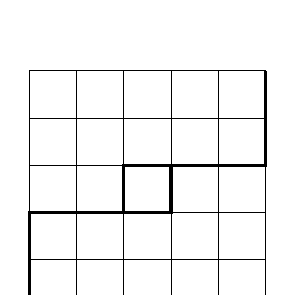
\begin{tikzpicture}[scale=3]
\draw (0,0) rectangle (1,1);
\draw[black,very thick] (0,0) -- (0,0.4)--(0.4,0.4)--(0.4,0.6)--(1,0.6)--(1,1);
\draw[black,very thick] (0.4,0.4)--(0.6,0.4)--(0.6,0.6);
\draw (0.2,0)--(0.2,1) (0.4,0)--(0.4,1) (0.6,0)--(0.6,1) (0.8,0)--(0.8,1);
\draw (0,0.2)--(1,0.2) (0,0.4)--(1,0.4) (0,0.6)--(1,0.6) (0,0.8)--(1,0.8); 
\end{tikzpicture}\]
Proceeding one small rectangle at a time, this deforms $u$ into $u'$ through a finite sequence of paths such that each step involves a homotopy in which the only change occurs within either $X_1$ or $X_2$. For such a restricted deformation, the points $\{x_i\}$ may be chosen so that the value of is unchanged. This completes
the proof.
\end{proof}
\begin{corollary}\label{van kampen coro}
Under the assumptions of Theorem~\ref{van kampen classic}, one has:
\begin{itemize}
\item If $X_2$ is simply connected then 
\[\pi_1(X_1,x)\to\pi_1(X,x)\]
is a surjection with kernel the normal subgroup generated by $\pi_1(i_1)(\pi_1(X,x))$.
\item If $X_0$ is simply connected then $\pi_1(X,x)$ is the free product of $\pi_1(X_1,x)$ and $\pi_1(X_2,x)$.
\item If $X_2$ and $X_0$ are simply connected then
\[\pi_1(X_1,x)\to\pi_1(X,x)\]
is an isomorphism.
\end{itemize}
\end{corollary}
\subsection{Graphs}
A graph is a CW complex of dimension $0$ or $1$. The $0$-cells of a graph are called its \textbf{vertices}, and the $1$-cells are called its edges. It follows from the definition of a CW complex that for each edge $e$, the set $\widebar{e}\setminus e$ consists of one or two vertices; if a vertex $v$ is contained in $\widebar{e}$, we say that $v$ and $e$ are \textbf{incident}. A \textbf{subgraph} is a subcomplex of a graph; thus if a subgraph contains an edge, it also contains the vertex or vertices incident with it.\par
An edge that is incident with only one vertex is called a \textbf{self-loop}. If two or more edges are incident with the same one or two vertices, they are called \textbf{multiple edges}. A graph with no self-loops or multiple edges is called a \textbf{simple graph}. (Some graph theory texts reserve the term graph to refer to a simple graph, in which case the more general kind of graph defined here is usually called a multigraph.)\par
An \textbf{edge path} in a graph is a finite sequence $(v_0,e_1,v_1,\cdots,v_{k-1},e_k,v_k)$ that starts and ends with vertices and alternates between vertices and edges, such that for each $i$, $\{v_{i-1},v_i\}$ is the set of vertices incident with the edge $e_i$. (Thus $v_{i-1}=v_i$ if and only if $e_i$ is a self-loop.) The vertices $v_0$ and $v_k$ are called the \textbf{initial vertex} and \textbf{terminal vertex} of the edge path, respectively, and we say it is an edge path from $v_0$ to $v_k$. We also allow a \textbf{trivial edge path} $(v_0)$ consisting of one vertex alone. An edge path is said to be \textbf{closed} if $v_0=v_k$, and \textbf{simple} if no edge or vertex appears more than once, except that $v_0$ might be equal to $v_k$.\par
A \textbf{cycle} is a nontrivial simple closed edge path. A \textbf{tree} is a connected graph that contains no cycles. A tree cannot contain self-loops or multiple edges: if $e$ is a self-loop incident with the vertex $v$, then $(v,e,v)$ is a cycle; and if $e'$ and $e''$ are two edges incident with the vertices $v'$ and $v''$, then $(v',e',v'',e'',v')$ is a cycle. It follows that every tree is a simple graph.
\begin{figure}[htpb]
\centering
\begin{minipage}{200pt}
\centering
\includegraphics{Graph-eg1}
\caption{A graph with three cycles.}
\end{minipage}
\hspace{20pt}
\begin{minipage}{200pt}
\centering
\includegraphics{Graph-eg2}
\caption{A tree.}
\end{minipage}
\end{figure}
\begin{proposition}\label{tree contractible}
Every finite tree is contractible, and thus simply connected.
\end{proposition}
\begin{proof}
Let $T$ be a finite tree. The proof is by induction on the number of edges in $T$. If there are no edges, then $T$ consists of a single vertex and is therefore contractible.
So assume every tree with $n$ edges is contractible, and let $T$ be a tree with $n+1$
edges.\par
Because $T$ is a simple graph, every edge of $T$ is incident with exactly two vertices.
If every vertex in $T$ is incident with at least two edges, then arguing exactly as in the proof of the classification theorem for $1$-manifolds, we can construct doubly infinite sequences $(v_j)_{j\in\Z}$ of vertices and $(e_j)_{j\in\Z}$ of edges such that for each $j$, $v_{j-1}$ and $v_j$ are the two vertices incident with $e_j$, and $e_j$, $e_{j+1}$ are two different edges incident with $v_j$. Because $T$ is finite, there must be some integers $n$ and $n+k>n$ such that $v_n=v_{n+k}$. If $n$ and $k$ are chosen so that $k$ is the minimum positive integer with this property, this means that $(v_n,e_{n+1},\cdots,e_{n+k},v_{n+k})$ is a cycle, contradicting the assumption that $T$ is a tree. Thus there must be a vertex $v$ that is incident with at most one edge. Since $T$ is connected, $v$ is incident with exactly one edge, say $e$, and $e$ is incident with exactly one other vertex $v'$.\par 
Let $T'$ be the subgraph of $T$ with the vertex $v$ and the edge $e$ deleted. The constant map from $\widebar{e}$ onto $\{v'\}$ is a strong deformation retraction; extending this to be the identity on $T'$ yields a strong deformation retraction of $T$ onto $T'$. Therefore, $T$ is homotopy equivalent to $T'$, which is contractible by the induction hypothesis.
\end{proof}
Let $\Gamma$ be a graph. A \textbf{spanning tree} in $\Gamma$ is a subgraph that is a tree and that contains every vertex of $\Gamma$.
\begin{proposition}
Every finite connected graph contains a spanning tree.
\end{proposition}
\begin{proof}
Let $\Gamma$ be a finite connected graph. If $\Gamma=\emp$, then the empty subgraph is
a spanning tree. Otherwise, we begin by showing that $\Gamma$ contains a \textbf{maximal tree}, meaning a subgraph that is a tree and is not properly contained in any larger tree in $\Gamma$. To prove this, start with any nonempty tree $T_0\sub\Gamma$ (e.g., a single vertex). If it is not maximal, then it is contained in a strictly larger tree $T_1$. Continuing in this way by induction, we obtain a sequence of trees $T_0\sub T_1\sub\cdots$, each properly contained in the next. Because $\Gamma$ is finite, the process cannot go on forever, so eventually we obtain a tree $T\sub\Gamma$ that is not contained in any strictly larger tree.\par
To show that $T$ is a spanning tree, suppose for the sake of contradiction that there
is a vertex $v\in\Gamma$ that is not contained in $T$. Because $\Gamma$ is connected, there is an edge path from a vertex $v_0\in T$ to $v$, say $(v_0,e_1,\cdots,e_k,v_k=v)$. Let $v_i$ be the last vertex in the edge path that is contained in $T$. Then the edge $e_{i+1}$ is not contained in $T$, because if it were, $v_{i+1}$ would also be in $T$ because $T$ is a subgraph. The subgraph $T'=T\cup\widebar{e}_{i+1}$ properly contains $T$, so it is not a tree, and therefore contains a cycle. This cycle must include $e_{i+1}$ or $v_{i+1}$, because otherwise it would be a cycle in $T$. However, since $e_{i+1}$ is the only edge of $T'$ that is incident with $v_{i+1}$, there can be no such cycle.
\end{proof}
Let $\Gamma$ be a finite connected graph. We construct a set of generators for the fundamental group of $\Gamma$ as follows. Choose a vertex $v$ as base point, and let $T\sub\Gamma$ be a spanning tree. Let $e_1,\cdots,e_n$ be the edges of $\Gamma$ that are not in $T$, and for each $i$ let $\{w_i,w'_i\}$ be the set of vertices incident with $e_i$. (Thus $w_i=w'_i$ if $e_i$ is a self-loop.) We can choose paths $g_i$ and $h_i$ in $T$ from $v$ to $w_i$ and $w'_i$, respectively. Let $f_i$ denote the loop in $\Gamma$ obtained by first following $g_i$ from $v$ to $w_i$, then traversing $e_i$, and then following $\bar{h}_i$ from $w'_i$ back to $v$. Note that the path class is independent of the choices of $g_i$ and $h_i$, because any two paths in $T$ with the
same endpoints are path-homotopic.
\begin{figure}[htbp]
\centering
\includegraphics{fandamental-graph-1}
\caption{Generators for the fundamental group of a graph.}
\end{figure}
\begin{theorem}[Fundamental Group of a Finite Graph]\label{fund graph}
The fundamental group of a finite connected graph $\Gamma$ based at a vertex $v$ is the free group on the path classes $[f_1],\cdots,[f_n]$ constructed above.
\end{theorem}
\begin{proof}
We prove the theorem by induction on the number $n$ of edges in $\Gamma\setminus T$. If $n=0$, then $\Gamma$ is a tree and hence simply connected, so there is nothing 
to prove.\par
For $n=1$, we must show that $\Gamma$ is the infinite cyclic group generated by $[f_1]$. Let $T$ be the chosen spanning tree, and let $e$ be the single edge in 
$\Gamma\setminus T$. By assumption, there is a cycle $(v_0,e_1,\cdots,e_m,v_m)$ in $\Gamma$. This cycle must include the edge $e$, because otherwise it would be a 
cycle in $T$. The subgraph $C\sub\Gamma$ consisting of the union of the vertices and edges $\{v_0,e_1,\cdots,e_m,v_m\}$ is homeomorphic to $S^1$ by the same argument 
as in the proof of Theorem~\ref{class one mani}. We will show that inclusion $C\hookrightarrow\Gamma$ is a homotopy equivalence.\par
Let $K$ be the union of all the edges in $\Gamma\setminus C$ together with their vertices. Each component $K_i$ of $K$ is a connected subgraph of $\Gamma$ contained in $T$, and is therefore a tree (since a cycle in $K_i$ would also be one in $T$). Moreover, each such component shares at least one vertex $y_i$ with $C$ because $\Gamma$ is connected. In fact, it shares exactly one: if $K_i\cap C$ contained two vertices $y_i,y'_i$, it would be possible to find a cycle in $T$ by following an edge path in $K_i$ from $y_i$ to $y'_i$ followed by the edge path in $C$ from $y'_i$ to $y_i$ that does not contain $e$. (This is possible since $C\approx S^1$.)\par
Now define a strong deformation retraction of $\Gamma$ onto $C$ as follows: on each $K_i$, it is a strong deformation retraction of $K_i$ onto $y_i$, which exists since $K_i$ is contractible; and on $C$ it is the identity. The resulting map is continuous by the gluing lemma, and shows that $\Gamma\simeq S^1$.\par
It remains to show that the path class $[f_1]$ is a generator of $\pi_1(\Gamma,v)$. Let $z$ be any vertex in $C$. A path $a$ that starts at $z$ and traverses each edge of $C$ in order is clearly path-homotopic to the standard generator of $S^1\approx C$ (or its inverse). Choosing any path $b$ from $z$ to $v$ yields an isomorphism $\varPhi_b:\pi_1(\Gamma,z)\to\pi_1(\Gamma,v)$. Thus a generator of $\pi_1(\Gamma,v)$ is $\varPhi_b[a]=[\bar{b}\ast a\ast b]$. Since $\bar{b}\ast a\ast b$ is a path that
goes from $v$ to $w_1$, traverses e, and returns to $v$, it is homotopic to $f_1$. (Remember that the path class of $f_1$ is independent of which paths we choose from $v$ to $w_1$ and $w'_1$ .) This completes the proof in the case $n=1$.\par
Now let $n\geq1$, and assume the conclusion holds for every graph with $n$ edges in
the complement of a spanning tree. Let $\Gamma$ be a graph with a spanning tree $T\sub\Gamma$ such that $\Gamma\setminus T$ consists of $n+1$ edges $e_1,\cdots,e_{n+1}$. We apply the Seifert–Van Kampen theorem in the following way. For each $i=1,\cdots,n+1$, choose a point $x_i\in e_i$. Let $U=\Gamma\setminus\{x_1,\cdots,x_n\}$ and $V=\Gamma\setminus\{x_{n+1}\}$. Both $U$ and
$V$ are open in $\Gamma$, and just as before it is easy to construct deformation retractions to show that $U\cap V\simeq T$, $U\simeq T\cup e_{n+1}$ and $V\simeq\Gamma\setminus e_{n+1}$. By the inductive hypothesis, $\pi_1(V,v)=F([f_1],\cdots,[f_n])$ and $\pi_1(U,v)=F([f_{n+1}])$. Since $U\cap V$ is simply connected, Corollary~\ref{van kampen coro} shows that $\pi_1(\Gamma,v)$ is isomorphic to the free product of these two free groups, which in turn is isomorphic the free group on $F([f_1],\cdots,[f_{n+1}])$ as claimed.
\begin{figure}[htbp]
\centering
\includegraphics{fandamental-graph-2}
\end{figure}
\end{proof}
\subsection{Fundamental Groups of CW Complexes}
Our next application of the Seifert–Van Kampen theorem is to give an algorithm for computing a presentation of the fundamental group of a finite CW complex.We have already taken care of the case of a complex of dimension $0$ or $1$ in our treatment
of graphs above. The next step is to examine the consequence of attaching cells of
higher dimensions.\par
We begin with $2$-cells. Although the details of the proof are a bit involved, the basic idea is that when a $2$-cell is attached to a space $X$, the attaching map can be thought of as the circle representative for an element of $\pi_1(X)$, and attaching the cell kills that element because it becomes null-homotopic in the adjunction space.
\begin{proposition}[\textbf{Attaching a Disk}]\label{attaching disk}
Let $X$ be a path-connected topological space, and let $\widetilde{X}$ be the space obtained by attaching a closed $2$-cell $D$ to $X$ along an attaching map $\varphi:\partial D\to X$. Let $v\in\partial D$, $\widetilde{v}=\varphi(v)\in X$ and $\gamma=\varphi_*(\alpha)\in\pi_1(X,\widetilde{v})$, where $\alpha$ is a generator of the infinite cyclic group $\pi_1(\partial D,v)$ Then the homomorphism $\pi_1(X,\widetilde{X})\to\pi_1(\widetilde{X},\widetilde{v})$ induced by inclusion $X\hookrightarrow\widetilde{X}$ is surjective, and its kernel is the smallest normal subgroup containing $\gamma$. If $\pi_1(X,\widetilde{v})$ has a finite presentation
\[\pi_1(X,\widetilde{v})=\langle\beta_1,\cdots,\beta_n\mid\sigma_1,\cdots,\sigma_s\rangle.\]
then $\pi_1(\widetilde{X},\widetilde{v})$ has the presentation
\[\pi_1(\widetilde{X},\widetilde{v})=\langle\beta_1,\cdots,\beta_n\mid\sigma_1,\cdots,\sigma_s,\tau\rangle.\]
where $\tau$ is an expression for $\gamma\in\pi_1(X,\widetilde{v})$ in terms of $\{\beta_1,\cdots,\beta_n\}$.
\end{proposition}
\begin{figure}[htbp]
\centering
\includegraphics{attaching-disk}
\caption{Attaching a disk.}
\end{figure}
\begin{proof}
Let $q:X\amalg D\to\widetilde{X}$ be the quotient map. As usual, we identify $X$ with
its image under $q$, so we can consider $X$ as a subspace of $\widetilde{X}$. First we set up some notation. Choose a point $z\in\Int D$, set $U=\Int D$ and $V=X\amalg(D\setminus\{z\})$, and let $\widetilde{U}=q(U)$, $\widetilde{V}=q(V)\sub\widetilde{X}$. Since $U$ and $V$ are saturated open subsets,
the restrictions of $q$ to $U$ and $V$ are quotient maps, and their images $\widetilde{U},\widetilde{V}$ are open in $\widetilde{X}$. Moreover, $\widetilde{U}$ and $\widetilde{U}\cap\widetilde{V}$ are path-connected because they are continuous images of path-connected sets, and $\widetilde{V}$ is path-connected because it is the union of the pathconnected sets $X$ and $\widetilde{U}\cap\widetilde{V}$ that have the point $\widetilde{v}$ in common.\par
In order to apply the Seifert-Van Kampen theorem in this situation, we need to work with a base point in $\widetilde{U}\cap\widetilde{V}$. Choose $p\in\Int D\setminus\{z\}\approx\B^2\setminus\{0\}$, and let $c:I\to\Int D\setminus\{z\}$ be a loop based at $p$ whose path class generates $\pi_1(\Int D\setminus\{z\},p)$. Then
let $\widetilde{p}=q(p)\in\widetilde{U}\cap\widetilde{V}$, and $\widetilde{c}=q\circ c$. In general, we use symbols without tildes to denote sets, points, or paths in $D$, and the same symbols with tildes to denote their images in $\widetilde{X}$.\par
The restriction of $q$ to $U$ is a one-to-one quotient map and therefore a homeomorphism onto its image. Since $U$ is simply connected, so is $\widetilde{U}$. On the other hand, $\widetilde{U}\cap\widetilde{V}$ is the image under $q$ of the saturated open subset $\Int D\setminus\{z\}$, so $q:\Int D\setminus\{z\}\to\widetilde{U}\cap\widetilde{V}$ is an injective quotient map and thus a homeomorphism. It follows that $\pi_1(\widetilde{U}\cap\widetilde{V},\widetilde{p})$ is the infinite cyclic group generated by $[\widetilde{c}]$. Now Corollary~\ref{van kampen coro} implies that inclusion $\widetilde{V}\hookrightarrow\widetilde{X}$ induces a surjective map
\begin{align}\label{attaching idsk-1}
\pi_1(\widetilde{V},\widetilde{p})\to\pi_1(\widetilde{X},\widetilde{p}).
\end{align}
whose kernel is the normal closure of the cyclic subgroup generated by $[\widetilde{c}]$.\par
To complete the proof, we just need to relate the fundamental group of $\widetilde{V}$ with that of $X$. Combining a strong deformation retraction of $D\setminus\{z\}$ onto $\partial D$ with the identity map of $X$, we obtain a homotopy $H:V\times I\to V$ that yields a strong deformation retraction of $V$ onto $X\amalg\partial D$. Because $q\circ H$ respects the identifications made by $q\times id_I:V\times I\to\widetilde{V}\times I$, it descends to a strong deformation retraction of $\widetilde{V}$ onto $X$. Therefore the inclusion $X\hookrightarrow\widetilde{V}$ is a homotopy equivalence. Thus we can replace $\pi_1(\widetilde{V},\widetilde{v})$ with $\pi_1(X,\widetilde{v})$ in $(\ref{attaching idsk-1})$, and we still have a surjective homomorphism whose kernel is the smallest normal subgroup containing $\gamma$. The statement about presentations then follows from the definition of push out.
\end{proof}
The analogous result for higher-dimensional cells is much simpler.
\begin{proposition}[\textbf{Attaching an $\bm{n}$-cell}]\label{attaching n cell}
Let $X$ be a path-connected topological space, and let $\widetilde{X}$ be a space obtained by attaching an $n$-cell to $X$, with $n\geq3$. Then inclusion $X\hookrightarrow\widetilde{X}$ induces an isomorphism of fundamental groups.
\end{proposition}
\begin{proof}
We define open subsets $\widetilde{U},\widetilde{U}\cap\widetilde{V}$ just as in the preceding proof. In this case, $\widetilde{U}\cap\widetilde{V}$ is simply connected, because it is homeomorphic to $\B^n\setminus\{0\}$, and the result follows.
\end{proof}
Putting these results together, we obtain the following powerful theorem. For technical reasons, the computations are much simpler if we assume that the base point lies in the closure of each of the $2$-cells.
\begin{theorem}
Suppose $X$ is a connected finite CW complex, and $v$ is a point in the $1$-skeleton of $X$ that is contained in the closure of every $2$-cell. Let $\beta_1,\cdots,\beta_n$ be generators for the free group $\pi_1(X_1,v)$ $($$X_1$ is a graph$)$, and let $e_1,\cdots,e_k$ be the $2$-cells of $X$. For each $i=1,\cdots,k$, let $\Phi_i:D_i\to X$ be a characteristic map for $e_i$ that takes $v_i\in\partial D_i$ to $v$, let $\varphi_i=\Phi_i|_{\partial D_i}:\partial D_i\to X_1$ be the corresponding attaching map, let $\alpha_i$ be a generator of $\pi_1(\partial_i,v_i)$, and let $\sigma_i$ be an expression for $(\varphi_i)_*(\alpha_i)\in\pi_1(X,v)$ in terms of the generators $\{\beta_i\}$. Then $\pi_1(X,v)$ has the following presentation:
\[\pi_1(X,v)=\langle\beta_1,\cdots,\beta_n\mid\sigma_1,\cdots,\sigma_k\rangle\]
\end{theorem}
\begin{proof}
This follows immediately by induction from the two preceding propositions,
using the result of Exercise~\ref{CW minus n-cell}.
\end{proof}
\subsection{Fundamental Groups of Compact Surfaces}
The computations in this chapter allow us to compute the fundamental groups of all compact surfaces. Now it will become clear why we chose similar notations for surface presentations and group presentations.
\begin{theorem}
Let $M$ be a topological space with a polygonal presentation $\langle a_1,\cdots,a_n\mid W\rangle$ with one face, in which all vertices are identified to a single point. Then $\pi_1(M)$ has the presentation $\langle a_1,\cdots,a_n\mid W\rangle$.
\end{theorem}
\begin{proof}
As we have observed, a polygonal presentation determines a CW decomposition of $M$ in a natural way. Under the assumption that all the vertices are identified to a single point, the $1$-skeleton $M_1$ is a wedge sum of circles, one for each symbol in the presentation, and thus its fundamental group has the presentation $\langle a_1,\cdots,a_n\mid\emp\rangle$. The attaching map of the single $2$-cell maps the boundary of the polygon onto the loop in $M_1$ obtained by following the generators in the order specified by the word $W$. The result follows immediately from Proposition~\ref{attaching disk}.
\end{proof}
\begin{corollary}[\textbf{Fundamental Groups of Compact Surfaces}]
The fundamental groups of compact connected surfaces have the following presentations:
\begin{itemize}
\item[$(a)$] $\pi_1(S^2)=\langle\emp\mid\emp\rangle$ $($the trivial group$)$.
\item[$(b)$] $\pi_1(T^2\#\cdots\#T^2)=\langle\beta_1,\gamma_1,\cdots,\beta_n,\gamma_n\mid\beta_1\gamma_1\beta_1^{-1}\gamma_1^{-1}\cdots\beta_n\gamma_n\beta_n^{-1}\gamma_n^{-1}=1\rangle$.
\item[$(c)$] $\pi_1(\P^2\#\cdots\#\P^2)=\langle\beta_1,\cdots,\beta_n\mid\beta_1^2\cdots\beta_n^2=1\rangle$.
\end{itemize}
\end{corollary}
In particular, for the torus this gives $\pi_1(T^2)=\langle\beta,\gamma\mid\beta\gamma=\gamma\beta\rangle=\Z^2$, which agrees with the result we derived earlier. In the case of the projective plane, this gives $\pi_1(\P^2)=\langle\beta\mid\beta^2=1\rangle=\Z/2\Z$.\par
The quotient group $G/[G,G]$ is denoted by $Ab(G)$ and called the \textbf{abelianization} of $G$. Because an isomorphism $F:G_1\to G_2$ takes the commutator subgroup of $G_1$ to that of $G_2$, isomorphic groups have isomorphic abelianizations. The abelianization is the largest abelian quotient of $G$, or equivalently the largest abelian homomorphic image of $G$, in the sense that any other homomorphism into an abelian group factors through the abelianization.
\begin{proposition}
The fundamental groups of compact surfaces have the following abelianizations:
\begin{itemize}
\item[$(a)$] $Ab\big(\pi_1(S^2)\big)=\{0\}$.
\item[$(b)$] $Ab\big(\pi_1(\underbrace{T^2\#\cdots\#T^2}_{n})\big)=\Z^{2n}$.
\item[$(c)$] $Ab\big(\pi_1(\underbrace{\P^2\#\cdots\#\P^2}_{n})\big)=\Z^{n-1}\times\Z/2\Z$.
\end{itemize}
\end{proposition}
\begin{proof}
The case of the sphere is immediate. Consider next an orientable surface of genus $n$, and let
\[G=\langle\beta_1,\gamma_1,\cdots,\beta_n,\gamma_n\mid\beta_1\gamma_1\beta_1^{-1}\gamma_1^{-1}\cdots\beta_n\gamma_n\beta_n^{-1}\gamma_n^{-1}=1\rangle\]
be the fundamental group. Define a map $\varphi:G\to\Z^{2n}$ as follows. Let $e_i=(0,\cdots,1,\cdots,0)\in\Z^{2n}$ ($1$ in the $i$-th place), and set
\[\varphi(\beta_i)=e_i,\quad\varphi(\gamma_i)=e_{i+n}.\]
As a map from the free group $F(\beta_1,\gamma_1,\cdots,\beta_n,\gamma_n)$ into $\Z^{2n}$, this sends the element $\beta_1\gamma_1\beta_1^{-1}\gamma_1^{-1}\cdots\beta_n\gamma_n\beta_n^{-1}\gamma_n^{-1}$ to $(0,\cdots,0)$, so it descends to a homomorphism from $G$ to $\Z^{2n}$. By the characteristic property of the abelianization, it also descends to a homomorphism (still denoted by $\varphi$) from $Ab(G)$ to $\Z^{2n}$.\par
To go back the other way, define $\psi:\Z^{2n}\to Ab(G)$ by
\[\psi(e_i)=\begin{cases}
[\beta_i],&1\leq i\leq n;\\
[\gamma_{i-n}],&n+1\leq i\leq 2n.
\end{cases}\]
where the brackets on the right-hand side denote the equivalence class in $Ab(G)$,
and extend it to be a homomorphism. It is easy to check that $\psi$ and $\varphi$ are inverses of each other.\par
Next consider a connected sum of projective planes, and write the fundamental group as
\[H=\langle\beta_1,\cdots,\beta_n\mid\beta_1^2\cdots\beta_n^2=1\rangle.\]
Let $f$ denote the nontrivial element of $\Z/2\Z$, and define $\varphi:Ab(H)\to\Z^{n-1}\times\Z/2\Z$ by
\[\varphi(\beta_i)=\begin{cases}
e_i,&1\leq i\leq n-1;\\
f-e_1-\cdots-e_{n-1},&i=n.
\end{cases}\]
As before, $\varphi(\beta_1^2\cdots\beta_n^2)=(0,\cdots,0)$ by direct computation (noting that $f+f=0$), so $\varphi$ gives a well-defined map from $H$ that descends to $Ab(H)$. The homomorphism $\psi:\Z^{n-1}\times\Z/2\Z\to Ab(H)$ defined by
\[\psi[e_i]=\beta_i,\quad\psi[f]=[\beta_1\cdots\beta_n].\]
is easily verified to be an inverse for $\varphi$.
\end{proof}
\begin{theorem}
Every nonempty, compact, connected $2$-manifold is homeomorphic to exactly one of the surfaces $S^2$, $T^2\#\cdots\#T^2$, or $\P^2\#\cdots\#\P^2$.
\end{theorem}
Recall that a compact $2$-manifold is said to be orientable if it admits an oriented presentation.
\begin{corollary}
A connected sum of projective planes is not orientable.
\end{corollary}
\begin{corollary}
Orientability of a compact surface is a topological invariant.
\end{corollary}
\begin{corollary}
The Euler characteristic of a surface presentation is a topological invariant.
\end{corollary}
Because of this corollary, if $M$ is a compact surface, we can define the Euler
characteristic of $M$, denoted by $\chi(M)$, to be the Euler characteristic of any presentation of that surface.
\subsection{Exercise}
\begin{exercise}
Compute the fundamental group of the two-holed torus $($the compact surface of genus $2$ obtained by sewing together two tori along the boundaries of an open disk removed from each$)$.
\end{exercise}
\begin{proof}
Denote the cited space by $X$, and take $T_1$ and $T_2$ to be its cover, where $T_1$, $T_2$ are both copies of tori. Since we have $\pi_1(T^2)\simeq\Z^2$, and $\pi_1(S^1)=0$. We obtain from van kampen theorem that
\[\pi_1(X)\simeq\Z^2\ast\Z^2\]
\end{proof}
\begin{exercise}
The Klein bottle $K$ is the quotient space of $S^1\times I$ obtained by identifying $(z,0)$ with $(z^{-1},1)$ for $z\in S^1$. Compute $\pi_1(K)$.
\end{exercise}
\begin{proof}
Consider the cover by two mobious strips. Their intersection can be viewd as the boundary of one of them. As travelling one time along the boundary is in fact travelling the strip twice, the image of the generater of the fundamental group of the boundary $a$ is $a^2$. Thus by van kampen theorem we get
\[\pi_1(K)\simeq F(a,b)/(a^2b^{-2})\]
\end{proof}
\begin{exercise}
Let $X=\{(p,q)\mid p\neq-q\}\sub S^n\times S^n$. Define a map $f:S^n\to X$ by $f(p)=(p,p)$. Prove that $f$ is a homotopy equivalence.
\end{exercise}
\begin{proof}
Define $g:X\to S^n$ through
\[g(p,q)=\dfrac{p+q}{|p+q|}\]
then we check that $gf=id_{S^n}$, and
\[fg(p,q)=(\dfrac{p+q}{|p+q|},\dfrac{p+q}{|p+q|})\]
To show that this is homotopic to the identity, we define
\[H:X\times I\to X\]
as
\[H((p,q),t)=(\dfrac{p+qt}{|p+qt|},\dfrac{pt+q}{|pt+q|})\]
this gives a homotopy.
\end{proof}
\begin{exercise}
Let $\mathcal{C}$ be a category that has all coproducts and coequalizers. Prove that $\mathcal{C}$ is cocomplete $($has all colimits$)$. Deduce formally, by use of opposite categories, that a category that has all products and equalizers is complete.
\end{exercise}
\begin{proof}
Let $M:\mathcal{D}\to\mathcal{C}$ be a $\mathcal{D}$-shaped diagram. Write $I=\mathrm{Obj}(\mathcal{D})$ and $A=Arrows(\mathcal{D})$. Denote $s,t:A\to\mathcal{D}$ the source and target maps. Suppose $\coprod_{i\in I}M_i$ and $\coprod_{a\in A}M_{s(a)}$ exist. Suppose that the coequalizer of
\[\begin{tikzcd}
\coprod_{a\in A}M_{s(a)}\ar[r,shift left=0.5ex,"\phi"]\ar[r,shift right=0.5ex,swap,"\psi"]&\coprod_{i\in I}M_i
\end{tikzcd}\]
where the morphisms are determined on the components as follows
\[\psi(M_{s(a)})=M_{t(a)},\quad \phi(M_{s(a)})=M_{s(a)}\]
Then the coequalizer is the colimit of this diagram.
\end{proof}
\begin{exercise}
Let $X\sub\R^3$ be the union of the unit $2$-sphere with the line segment $\{(0,0,z):-1\leq z\leq 1\}$. Compute $\pi_1(X,N)$, where $N=(0,0,1)$ is the north pole, giving explicit generator$(s)$.
\end{exercise}
\begin{proof}
The fundamental group is isomorphic to $\Z$.
\end{proof}
\begin{exercise}
Show that any two vertices in a tree are joined by a unique simple edge path.
\end{exercise}
\begin{proof}
If this is not the case, there would be a cycle.
\end{proof}
\begin{exercise}\label{tree stong}
Show that every vertex in a finite tree is a strong deformation retract of the tree.
\end{exercise}
\begin{proof}
Choose a vertex $v$. At each step, choose a vertex other than $v$ that is incident with only one edge as in the proof of Proposition~\ref{tree contractible}, and retract this vertex along the edge. This gives a new tree with one vertex, one edge deleted. Arguing by induction gives the claim.
\end{proof}
\begin{exercise}
Compute the fundamental group of the complement of the three coordinate axes in $\R^3$, giving explicit generator$(s)$.
\end{exercise}
\begin{proof}
This space is homotopy equivalent to the $2$-sphere with six points removed, which is homotopy equivalent to the plane punctured with five points. And this space deforms to a bouquet of five circles. So the fundamental group is the free product of five $\Z$.
\end{proof}
\begin{exercise}\label{fund group connect sum}
Compute the fundamental group of a connect sum of two manifolds with dimension $\geq 3$.
\begin{itemize}
\item[$(a)$] Let $M_1\#M_2$ be a connected sum of $n$-manifolds $M_1$ and $M_2$. Show that there are open subsets $U_1,U_2\sub M_1\#M_2$ and points $p_i\in M_i$ such that $U_i\approx M_i\setminus\{p_i\}$, $U_1\cap U_2\approx\R^n\setminus\{0\}$, and $U_1\cup U_2=M_1\#M_2$.
\item[$(b)$] Suppose $M$ is a connected manifold of dimension at least $3$, and $p\in M$. Show that inclusion $M\setminus\{p\}\hookrightarrow M$ induces an isomorphism $\pi_1(M\setminus\{p\})\to\pi_1(M)$.
\item[$(c)$] Suppose $M$ and $N$ are connected $n$-manifolds with $n\geq 3$. Prove that the fundamental group of $M\#N$ is isomorphic to $\pi_1(M)\ast\pi_1(N)$.
\end{itemize}
\end{exercise}
\begin{proof}
$(a)$: Choose $U_1=M_1\#A_2$ where $A_2$ is an annulus. Then $U_1\approx M_1\setminus\{p_1\}$ since $A_1\approx\B^n\setminus\{0\}$. Similar for $U_2$.\par
$(b)$: Choose a coordinate ball around $p$, and use van kampen theorem for $M\setminus\{p\}$ and $U$. Since $U\setminus\{p\}$ is simply connected, we get the result.\par
$(c)$: Use $(a)$, since $U_1\cap U_2$ is simply connected, the claim follows from van kampen.
\end{proof}
\begin{exercise}
Suppose $M$ and $N$ are nonempty, compact, connected $2$-manifolds. Show that any two connected sums of $M$ and $N$ are homeomorphic, as follows:
\begin{itemize}
\item[$(a)$] Show that it suffices to prove that any two connected sums have isomorphic fundamental groups.
\item[$(b)$] Suppose $p,p'$ are points in $M$, and $U,U'\sub M$ are coordinate balls containing $p$ and $p'$, respectively. Show that there exist a homeomorphism
$F:M\setminus\{p\}\to M\setminus\{p'\}$ and a loop $f:I\to U$, such that $[f]$ generates $\pi_1(U\setminus\{p\})$ and $F\circ f$ generates $\pi_1(U'\setminus\{p'\})$.
\item[$(c)$] Use Exercise~\ref{fund group connect sum}$(a)$ to complete the proof.
\end{itemize}
\end{exercise}
\begin{proof}
$(a)$: By the classification theorem, it suffices to prove for the fundamental group.\par
$(b)$: $M\setminus\{p\}$ has a CW structure which is a graph. So $\pi_1(M\setminus\{p\})$ is a free group. Since $U\setminus\{p\}\approx\R^2\setminus\{0\}\approx U'\setminus\{p'\}$, the homeomorphism $F$ is easy to construct.\par
$(c)$: From Exercise~\ref{fund group connect sum}, the fundamental group of $M\#N$ is the push out of $\pi_1(M\setminus\{p\})$ and $\pi_1(N\setminus\{p\})$ where $p$ is in the pasted coordinate ball. Since the image of the generator of $\pi_1(U\setminus\{p\})$ into $\pi_1(M\setminus\{p\})$ are the same (by the homeomorphism in $(b)$), we conclude that the fundamental group of $M\#N$ is invariant.
\end{proof}
\begin{exercise}
Let $X_n$ be the union of the $n$ circles of radius $1$ that are centered at the points $\{0,2,4,\cdots,2n-2\}$ in $\C$, which are pairwise tangent to each other along the $x$-axis. Prove that $\pi_1(X_n,1)$ is a free group on $n$ generators, and describe explicit loops representing the generators.
\end{exercise}
\begin{proof}
$X_n$ is homotopy equivalent to a bouquet of $n$ circles.
\end{proof}
\begin{exercise}
Let $G$ be a finitely presented group. Show that there is a finite CW complex whose fundamental group is isomorphic to $G$.
\end{exercise}
\begin{exercise}
For each of the following spaces, give a presentation of the fundamental group together with a specific loop representing each generator.
\begin{itemize}
\item[$(a)$] A closed disk with two interior points removed.
\item[$(b)$] The projective plane with two points removed.
\item[$(c)$] A connected sum of $n$ tori with one point removed. 
\item[$(d)$] A connected sum of $n$ tori with two points removed.
\end{itemize}
\end{exercise}
\begin{proof}
$(a)$: This is figure eight, and the fundamental group is $\Z\ast\Z$.\par
$(b)$: Similar with the figure eight, but the two circle is guled, so this space is homotopy equivalent to $S^1$.\par
$(c)$: This is a bouquet of $n$ circles.\par
$(d)$: Thid is still a bouquet of $2n$ circles.
\end{proof}
\begin{exercise}
Show that a compact connected surface $M$ is nonorientable if and only if it contains a subset homeomorphic to the M\"obius band.
\end{exercise}
\begin{exercise}
Let $Q$ be the following annulus in the plane:
\[Q=\{z\in\C:1\leq|z|\leq 3\}\]
Let $\sim$ be the equivalence relation on $Q$ generated by
\[z\sim-z,\quad\text{if }z\in\partial Q.\]
Let $\widetilde{Q}=Q/\sim$, and let $q:Q\to\widetilde{Q}$ be the quotient map. Find a presentation for $\pi_1(\widetilde{Q},q(2))$, identifying specific loop$(s)$ representing the generator$(s)$.
\end{exercise}
\begin{proof}
This is a connect sum of two projective spaces.
\end{proof}
\begin{exercise}\label{Eular char graph}
Let $\Gamma$ be a finite connected graph. The Euler characteristic of $\Gamma$ is $\chi(\Gamma)=V-E$, where $V$ is the number of vertices and $E$ is the number of edges. Show that the fundamental group of $\Gamma$ is a free group on $1-\chi(\Gamma)$ generators. Conclude that $\chi(\Gamma)$ is a homotopy invariant, meaning that homotopy equivalent graphs have the same Euler characteristic.
\end{exercise}
\begin{proof}
First we show that the Euler characteristic of a finite tree is $1$. In fact, any tree con be reduced into a single vertex by the argument in the proof of Exercise~\ref{tree stong}. And each step does not change the Euler characteristic, so we get the claim since $\chi(v)=1$ for a single vertex.\par
Now for a grahph $\Gamma$, consider the spaning tree $T\sub\Gamma$. Since $T$ differs from $\Gamma$ only by some edges, we have $\chi(T)=\chi(\Gamma)+n$. Where $n$ is the number of the edges that is not in $T$. By Theorem~\ref{fund graph}, $\pi_1(\Gamma)$ has $n$ generetors. So $n=1-\chi(\Gamma)$. 
\end{proof}
\section{Covering spaces}
\subsection{The definition of covering spaces}
\begin{definition}
A space $X$ is said to be \textbf{locally path connected} if for any $x\in X$ and any neighborhood $U$ of $x$, there is a smaller neighborhood $V$ of $x$ each of whose points can be connected to $x$ by a path in $U$.
\end{definition}
This is equivalent to the seemingly more stringent requirement that the topology of $X$ have a basis consisting of path connected open sets. In fact, if $X$ is locally path connected and $U$ is an open neighborhood of a point $x$, then the set
\[V=\{y\mid y\text{ can be connected to $x$ by a path in $U$}\}\]
is a path connected open neighborhood of $x$ that is contained in $U$. Observe that if $X$ is connected and locally path connected, then it is path connected. \textit{Throughout this section, we assume that all given spaces are connected and locally path connected}.
\begin{definition}
Let $p:E\to X$ be a continuous map. An open subset $U$ of $X$ is said to be \textbf{evenly covered} by $p$ if the inverse image $p^{-1}(U)$ can be written as the union of disjoint open sets $V_\alpha$ in $E$ $($called the \textbf{sheets of the covering over $\bm{U}$}$)$ such that for each $\alpha$, the restriction of $p$ to $V_\alpha$ is a homeomorphism of $V_\alpha$ onto $U$. The collection $\{V_\alpha\}$ is called a partition of $p^{-1}(U)$ into slices.
\end{definition}
\begin{definition}
Let $p:E\to X$ be continuous and surjective. If every point of $X$ has a
neighborhood $U$ that is evenly covered by $p$, then $p$ is called a \textbf{covering map}, and $E$ is said to be a covering space of $X$.\par
We say that a path connected open subset $V$ with the property is a \textbf{fundamental neighborhood} of $X$. We call $E$ the total space, $X$ the base space, and $p^{-1}(x)$ a \textbf{fiber} of the covering $p$.
\end{definition}
\begin{proposition}[\textbf{Elementary Properties of Covering Maps}]
\mbox{}
\begin{itemize}
\item[$(a)$] Every covering map is a local homeomorphism, an open map, and a quotient
map.
\item[$(b)$] An injective covering map is a homeomorphism.
\item[$(c)$] A finite product of covering maps is a covering map.
\item[$(d)$] Let $p:E\to X$ be a covering map. If $X_0$ is a subspace of $X$, and if $E_0:=p^{-1}(X_0)$, then the map $p_0:E_0\to X_0$ obtained by restricting $p$ is a 
covering map.
\end{itemize}
\end{proposition}
\begin{proof}
Let $p:E\to X$ be a covering map.
\begin{itemize}
\item[$(a)$]That $p$ is a local homeomorphism is easliy verified from the definition. For the openness, suppose $A$ is an open set of $E$. Given $x\in p(A)$, choose a neighborhood $U$ of $x$ that is evenly covered by $p$ and let $\{V_\alpha\}$ be a partition of $p^{-1}(U)$ into slices. Then there is a point $y$ of $A$ such that $p(y)=x$; let $V_\beta$ be the slice containing $y$, then the set $V_\beta\cap A$ is open in $E$ and hence open in $V_\beta$; because $p$ maps $V_\beta$ homeomorphically onto $U$, the set $p(V_\beta\cap A)$ is open in $U$ and hence open in $X$; it is thus a neighborhood of $x$ contained in $p(A)$, as desired.\par 
Now since $p$ is a surjective continuous open map, it is a quotient map.
\item[$(b)$]If $p$ is injective, then it is a bijective open continuous map, hence a homeomorphism.
\item[$(d)$]Given $x_0\in X_0$, let $U$ be an open set in $X$ containing $x_0$ that is evenly covered by $p$; let $\{V_\alpha\}$ be a partition of $p^{-1}(U)$ into slices. 
Then $U\cap X_0$ is a neighborhood of $x_0$ in $X_0$, and the sets $V_\alpha\cap E_0$ are disjoint open sets in $E_0$ whose union is $p^{-1}(U\cap X_0)$, and each is 
mapped homeomorphically onto $U\cap X_0$ by $p$.
\end{itemize} 
\end{proof}
\begin{example}
The exponential quotient map $\eps:\R\to S^1$ given by $\eps(x)=e^{2\pi ix}$ is a covering map
\end{example}
\begin{example}
The $n$-th power map $p_n:S^1\to S^1$ given by $p_n(z)=z^n$ is also a covering map. For 
each $z_0\in S^1$, the set $U=S^1-\{z_0\}$ has preimage equal to $\{z\in S^1:z^n\neq z_0\}$, which 
has $n$ components, each of which is an open arc mapped homeomorphically by $p_n$ onto $U$.
\end{example}
\begin{example}
Each $f_n=z^n:S^1\to S^1$ is a cover. The projection $S^n\to\RP^n$ is a cover, where the real projective space $\RP^n$ is obtained from $S^n$ by identifying antipodal 
points.
\end{example}
\begin{example}
If $p:E\to X$ is a cover, $f:Y\to X$ is a map $($where $Y$ is connected and locally path connected$)$, consider the pull back of $f$ and $p$:
\[\begin{tikzcd}
Y\times_{X}E\ar[d,"p'"]\ar[r,"f'"]&E\ar[d,"p"]\\
Y\ar[r,"f"]&X
\end{tikzcd}\]
Then $p'$ is also a cover.
\end{example}
It is important to realize that a surjective local homeomorphism need not be a
covering map, as the next example shows.
\begin{example}
Let $E$ be the interval $(0,2)\sub\R$, and define $f:E\to S^1$ by $f(x)=e^{2\pi ix}$. Then $f$ is 
a local homeomorphism (because it is the restriction of the covering map $\eps$), and is clearly 
surjective. However, $f$ is not a covering map, as the point $1\in S^1$ has no evenly covered neighborhood.
\begin{figure}[htbp]
\centering
\includegraphics{covering-counter}
\caption{A surjective local homeomorphism that is not a covering map.}
\end{figure}
\end{example}
In contrast to the example above, a local homeomorphism is indeed a covering map under center conditions. Then following result will be used when we consider covering 
spaces of manifolds.
\begin{proposition}
A proper local homeomorphism between connected, locally path-connected, and compactly generated Hausdorff spaces is a covering map.
\end{proposition}
\begin{proof}
Because $\pi$ is a local diffeomorphism, it is an open map, and because it is proper, it is a closed map (compactly generated Hausfordd space). Thus $\pi(E)$ is both 
open and closed in $M$. Since it is obviously nonempty, it is all of $M$, so $\pi$ is surjective.\par
Let $q\in M$ be arbitrary. Since $\pi$ is a local diffeomorphism, each point of $\pi^{-1}(q)$ has a neighborhood on which $\pi$ is injective, so $\pi^{-1}(q)$ is a 
discrete subset of $E$. Since $\pi$ is proper, $\pi^{-1}(q)$ is also compact, so it is finite. Write $\pi^{-1}(q)=\{p_1,\dots,p_k\}$. For each $i$, there exists a 
neighborhood $V_i$ of $p_i$ on which $\pi$ is a diffeomorphism onto an open subset $U_i\sub M$. Shrinking each $V_i$ if necessary, we may assume also that 
$V_i\cap V_j=\emp$ for $i\neq j$.\par
Now let $U=\bigcap_{i=1}^{k}U_i$, which is a neighborhood of $q$. Then $U\sub U_i$ for all $i$. Because $K:=E-\bigcup_{i=1}^{k}V_i$ is closed in $E$ and $\pi$ is a 
closed map, $\pi(K)$ is closed in $M$. Replacing $U$ by $U-\pi(K)$, we can assume that $U$ also satisfies $\pi^{-1}(U)\sub\bigcup_{i=1}^{k}V_i$. Finally, after replacing 
$U$ by the connected component of $U$ containing $q$, we can assume that $U$ is connected. We will show that $U$ is evenly covered.\par
Let $\widetilde{V}_i=\pi^{-1}(U)\cap V_i$. Then $\pi^{-1}(U)=\widetilde{V}_1\cup\cdots\cup\widetilde{V}_k$. Because $\pi|_{V_i}:V_i\to U_i$ is a diffeomorphism, 
$U\sub U_i$ implies that $\pi|_{\widetilde{V}_i}:\widetilde{V}_i\to U$ is still a diffeomorphism, and in particular $\widetilde{V}_i$ is connected. Because 
$\widetilde{V}_1,\dots,\widetilde{V}_k$ are disjoint connected open subsets of $\pi^{-1}(U)$, they are exactly the components of $\pi^{-1}(U)$.
\end{proof}
For the properness condition, we have the following useful result.
\begin{proposition}
A covering map is proper if and only if it is finite-sheeted.
\end{proposition}
\begin{proof}
Since $\{y\}$ is compect, the fiber $f^{-1}(y)$ is compect, and so it is finite.\par
If $p$ is finite-sheeted, assume $K\sub X$ is compact and let $L:=p^{-1}(K)$, we need to show $L$ is compact. Assume that $\{U_\alpha\}$ is an open cover of $L$. For 
each $x\in K$, choose a fundamental neighborhood $V_x$ such that each component of $p^{-1}(V_x)$ is contained in some $U_\alpha$. This can be done by suitable shrinking 
since $p^{-1}(V_x)$ has finitely many components. Then $K$ has a finite cover $\{V_{x_i}\}_{i=1}^{m}$, and
\[L=p^{-1}(K)\sub p^{-1}(\bigcup_{i=1}^{m}V_{x_i})=\bigcup_{i=1}^{m}p^{-1}(U_{x_i}).\]
Since each $p^{-1}(U_{x_i})$ is contained in a $U_\alpha$, this gives a finite subcover of $\{U_\alpha\}$.
\end{proof}
If $p:X\to Y$ is any surjective continuous map, a \textbf{section} of $p$ is a continuous map $\sigma:Y\to X$ such that $p\circ\sigma=id_Y$ (i.e., a right inverse for $p$). If $U\sub Y$ is an open subset, a \textbf{local section} of $p$ over $U$ is a continuous map $\sigma:U\to X$ such that $p\circ\sigma=id_U$.
\begin{proposition}[\textbf{Existence of Local Sections}]
Let $p:E\to X$ be a covering map. Given any evenly covered open subset $U\sub X$, any $x\in U$, and any $e_0$ in the fiber over $x$, there exists a local section $\sigma:U\to E$ such that $\sigma(x)=e_0$.
\end{proposition}
\begin{proof}
Let $\widetilde{U}_0$ be the sheet of $p^{-1}(U)$ containing $e_0$. Since the restriction of $p$ to $\widetilde{U}_0$ is a homeomorphism, we can just take $\sigma=(p|_{\widetilde{U}_0})^{-1}$.
\end{proof}
\begin{proposition}[\textbf{Cardinality of the fiber}]
For every covering map $p:E\to X$, the cardinality of the fibers $p^{-1}(x)$ is the same for all fibers.
\end{proposition}
\begin{proof}
Define an equivalence relation on $X$ by saying that $x\sim x'$ if and only if $p^{-1}(x)$ and $p^{-1}(x')$ have the same cardinality. Suppose $x\in X$, and let $U$ be an evenly covered neighborhood of $x$. Then each sheet of $p^{-1}(x)$ contains exactly one point of each fiber, so for any $x'\in U$, there are one-to-one correspondences
\[p^{-1}(x)\Longleftrightarrow\text{sheet of }p^{-1}(U)\Longleftrightarrow p^{-1}(x')\]
which shows that $x'\sim x$. It follows that $U$ is contained in the equivalence class
$[x']$, so each equivalence class is open. Thus by the connectness of $X$, there is just one equivalence class.
\end{proof}
If $p:E\to X$ is a covering map, the cardinality of any fiber is called the \textbf{number
of sheets of the covering}.
\subsection{The unique lifting property}
\begin{theorem}[\textbf{Unique Lifting Property}]\label{lift prop}
Let $p:E\to X$ be a covering map. Suppose $Y$ is connected, $\varphi:Y\to X$ is continuous, and $\widetilde{\varphi}_1,\widetilde{\varphi}_2:Y\to E$ are lifts of
$\varphi$ that agree at some point of $Y$. Then $\widetilde{\varphi}_1$ is identically equal to $\widetilde{\varphi}_2$.
\end{theorem}
\begin{proof}
Let $\mathcal{A}=\{x\in X\mid \widetilde{\varphi}_1(x)=\widetilde{\varphi}_2(x)\}$. By hypothesis $\mathcal{A}$ is not empty. Since $X$ is connected, if we can show that $\mathcal{A}$ is open and closed in $X$, it must be all of $X$.\par
To show that $\mathcal{A}$ is open, suppose $x\in\mathcal{A}$. Write $r=\widetilde{\varphi}_1(x)=\widetilde{\varphi}_2(x)$ and $z=p(r)=\varphi(x)$. Let $U\sub X$ be an evenly covered neighborhood of $z$, and let $\widetilde{U}$ be the
component of $p^{-1}(U)$ containing $r$. If we set $V=\widetilde{\varphi}_1^{-1}(\widetilde{U})\cap\widetilde{\varphi}_2^{-1}(\widetilde{U})$, then $V$ is a neighborhood of $x$ on which both $\widetilde{\varphi}_1$ and $\widetilde{\varphi}_3$ take their values in $\widetilde{U}$. Now, the fact that $\widetilde{\varphi}_1$ and $\widetilde{\varphi}_2$ are lifts of $\varphi$ translates to $\varphi=p\circ\widetilde{\varphi}_1=p\circ\widetilde{\varphi}_2$. Since $p$ is
injective on $\widetilde{U}$, we conclude that $\widetilde{\varphi}_1$ and $\widetilde{\varphi}_2$ agree on $V$, which is to say that $V\sub\mathcal{A}$, so $\mathcal{A}$ is open.\par
To show that $\mathcal{A}$ is closed, we show that its complement is open. Suppose $x\notin\mathcal{A}$, and set $r_1=\widetilde{\varphi}_1(x)$ and $r_2=\widetilde{\varphi}_2(x)$, so that $r_1\neq r_2$. As above, let $z=p(r_1)=p(r_2)=\varphi(x)$, and let $U$ be an evenly covered neighborhood of $z$. If $\widetilde{U}_1$ and $\widetilde{U}_2$ are the components of $p^{-1}(U)$ containing $r_1$ and $r_2$, respectively, then $\widetilde{U}_1\cap\widetilde{U}_2=\emp$, and $p$ restricts to a homeomorphism from $\widetilde{U}_1$ to $U$ and from $\widetilde{U}_2$ to $U$. Setting $V=\widetilde{\varphi}_1^{-1}(\widetilde{U})\cap\widetilde{\varphi}_2^{-1}(\widetilde{U})$ we conclude that $\widetilde{\varphi}_1(V)\sub\widetilde{U}_1$ and $\widetilde{\varphi}_2(V)\sub\widetilde{U}_2$, so $\widetilde{\varphi}_1\neq \widetilde{\varphi}_2$ on $V$, which is to say that $V\sub X\setminus\mathcal{A}$. Thus $\mathcal{A}$ is closed, and the proof is complete.
\end{proof}
\begin{theorem}[\textbf{Homotopy Lifting Property}]\label{homotopy lift}
Let $p:E\to X$ be a covering map, and let $Y$ be a locally connected space. Suppose $\varphi_0,\varphi_1:Y\to X$ are continuous maps, $H:Y\times I\to X$ is a homotopy from $\varphi_0$ to $\varphi_1$, and $\widetilde{\varphi}_0:Y\to E$ is any lift of $\varphi_0$. Then there exists a unique lift of $H$ to a homotopy $\widetilde{H}$ satisfying $\widetilde{H}_0=\widetilde{\varphi}_0$. If $H$ is stationary on some subset $A\sub Y$, then so is $\widetilde{H}$.
\end{theorem}
\begin{proof}
We begin by proving a local form of uniqueness for $\widetilde{H}$. Suppose $W$ is any
subset of $Y$, and $\widetilde{H}$, $\widetilde{H}'$ are lifts of $H$ defined on $W\times I$ that agree on $W\times\{0\}$. Then for each $y\in W$, the two maps $t\mapsto\widetilde{H}(y,t)$ and $t\mapsto\widetilde{H}'(y,t)$ are lifts of the path
$t\mapsto H(y,t)$ starting at the same point, so they agree by the unique lifting property. It follows that $\widetilde{H}$ and $\widetilde{H}'$ agree on $W\times I$. In particular, taking $W=Y$, we see that a globally defined lift $\widetilde{H}:Y\times I\to E$ satisfying $\widetilde{H}_0=\widetilde{\varphi}_0$ is unique if it exists.\par
To prove existence, let $y_0\in Y$ be arbitrary. We begin by defining $\widetilde{H}$ on $W\times I$ for some neighborhood $W$ of $y_0$. For each $s\in I$, there exists an evenly covered neighborhood $U$ of the point $H(y_0,s)\in X$. Because $H^{-1}(U)$ is a neighborhood of $(y_0,s)$ and product open subsets form a basis for the product topology on $Y\times I$, there exist open subsets $V\sub Y$ and $J\sub I$ such that $(y_0,s)\in V\times J\sub W\times I$. The collection of all such product sets $V\times J$ is an open cover of $\{y_0\}\times I$, so by compactness finitely many of them, say $V_1,J_1,\cdots,V_m,J_m$, cover $\{y_0\}\times I$. Let $W$ be a connected neighborhood of $y_0$ contained in $V_1\cap\cdots\cap V_m$ (such a neighborhood exists by local connectedness), and let $\delta$ be a Lebesgue number for the open cover $\{J_1,\cdots,J_k\}$ of $I$. If $n$ is a positive integer such that $1/n<\delta$, it follows that for each $j=1,\cdots,n$, the set $W\times[(j-1)/n,j/n]$ is mapped by $H$ into an evenly covered open subset of $X$.\par
We define a lift of $H$ on $W\times I$ inductively as follows. First, choose an evenly
covered open subset $U_1\sub X$ containing $H(W\times[0,1/n])$, and let $\sigma_1:U_1\to E$ be the local section of $p$ satisfying $\sigma_1(\varphi_0(y_0))=\widetilde{\varphi}_0(y_0)$. For $(y,s)\in W\times[0,1/n]$,
define $\widetilde{H}(y,s)=\sigma_1\circ H(y,s)$. This is a composition of continuous maps, and is thus continuous. The map $\widetilde{H}_0:W\to E$ given by $\widetilde{H}_0(y)=H(y,0)$ is a lift of $H_0=\varphi_0$ on a connected domain that agrees with $\widetilde{\varphi}_0$ at the point $y_0$, so by uniqueness of lifts
it agrees with $\varphi_0$ on all of $W$.\par
Now suppose by induction that a continuous lift $\widetilde{H}$ has been defined on $W\times[0,(j-1)/n]$ for some $j\in\{1,\cdots,n\}$. Let $U_j$ be an evenly covered open subset containing $H(W\times[0,(j-1)/n])$ and let $\sigma_j:U_j\to E$ be the local section satisfying $\sigma_j(H(y_0,(j-1)/n))=\widetilde{H}(y_0,(j-1)/n)$. Define $\widetilde{H}(y,s)=\sigma_j\circ H(y,s)$ for $(y,s)\in W\times[(j-1)/n,j/n]$, which is continuous by composition. We need to show that it agrees with our previous definition where the two domains overlap, namely for $(y,s)\in W\times\{(j-1)/n\}$. Note that this set is connected (because $W$ is), and the restrictions to this set of the old and new definitions of $\widetilde{H}$ are both lifts of $H$ that agree at the point $(y_0,(j-1)/n)$. Thus by uniqueness of lifts, they agree everywhere that both are defined. By the pasting lemma, therefore, we obtain a continuous lift of $H$ defined on $W\times[0,j/n]$. This completes the induction and proves that $H$ has a continuous lift on $W\times I$.\par
Every point of $Y$ is contained in some neighborhoodW such that $H$ can be lifted
to $W\times I$. If $W$ and $W'$ are any two such neighborhoods, then the corresponding lifts $\widetilde{H}$ and $\widetilde{H}'$ agree on $(W\cap W')\times I$ by the local uniqueness property proved in the first paragraph. It follows from the pasting lemma that $\widetilde{H}$ is globally well defined and continuous, and by construction it is a lift of $H$ satisfying $\widetilde{H}_0=\widetilde{\varphi}_0$.\par
Finally, if $H$ is stationary on $A\sub Y$, then for each $a\in A$, the path $t\mapsto H(a,t)$ is a constant path at $\varphi_0(a)$ whose unique lift starting at $\widetilde{\varphi}_0(a)$ is the constant path $t\mapsto\widetilde{\varphi}(a)$. It follows that $\widetilde{H}$ is also stationary on $A$.
\end{proof}
\begin{corollary}[\textbf{Path Lifting Property}]\label{path lift}
Let $p:E\to X$ be a covering map. Suppose $f:I\times X$ is any path, and $e\in E$ is any point in the fiber of $p$ over $f(0)$. Then there exists a unique lift $\widetilde{f}:I\to E$ of $f$ such that $\widetilde{f}(0)=e$.
\end{corollary}
\begin{proof}
A path $f$ can be viewed as a homotopy between two maps from a onepoint space $\{\ast\}$ into $S^1$, namely $\ast\mapsto f(0)$ and $\ast\mapsto f(1)$. Thus the existence and uniqueness of $\widetilde{f}$ follow from the homotopy lifting property.
\end{proof}
Whenever $p:E\to X$ is a covering map, we use the following notation for lifts of paths: if $f:I\to X$ is a path and $e\in p^{-1}(f(0))$ then $\widetilde{f}_e:I\to E$ denotes the unique lift of $f$ satisfying $\widetilde{f}_e(0)=e$.
\begin{theorem}[\textbf{Monodromy Theorem}]
Let $p:E\to X$ be a covering map. Suppose $f$ and $g$ are paths in $X$ with the same initial point and the same terminal point, and $\widetilde{f}_e$, $\widetilde{g}_e$ are their lifts with the same initial point $e\in E$.
\begin{itemize}
\item[$(a)$]$\widetilde{f}_e\simeq\widetilde{g}_e$ if and only if $f\simeq g$.
\item[$(a)$]If $f\simeq g$, then $\widetilde{f}_e(1)\simeq\widetilde{g}_e(1)$.
\end{itemize}
\end{theorem}
\begin{proof}
If $\widetilde{f}_e\simeq\widetilde{g}_e$, then $f\simeq g$ because composition with $p$ preserves path homotopy.\par
Conversely, suppose $f\simeq g$, and let $H:I\times I\to X$ be a path homotopy between
them. Then the homotopy lifting property implies that $H$ lifts to a homotopy $H:I\times I\to E$ between $\widetilde{f}$ and some lift of $g$ starting at $e$, which must be equal to $\widetilde{g}$ by the unique lifting property. This proves $(a)$. To prove $(b)$, just note that $f\simeq g$ implies that $\widetilde{f}_e$ and $\widetilde{f}_e$ are path-homotopic by $(a)$, so they have the same terminal point.
\end{proof}
\begin{theorem}[\textbf{Injectivity Theorem}]
Let $p:E\to X$ be a covering map. For any point $e\in E$, the induced homomorphism $p_*:\pi_1(E,e)\to\pi_1(X,p(e))$ is injective.
\end{theorem}
\begin{proof}
Suppose $[f]\in\pi_1(E,e)$ is in the kernel of $p_*$. This means that $p_*[f]=[c_x]$,
where $x=p(e)$. In other words, $p\circ f\simeq c_x$ in $X$. By the monodromy theorem, therefore, any lifts of $p\circ f$ and $c_x$ that start at the same point must be path-homotopic in $E$. Now, $f$ is a lift of $p\circ f$ starting at $e$, and the constant loop $c_e$ is a lift of $c_x$ starting at the same point; therefore, $f\simeq c_e$ in $E$, which means that $[f]=1$.
\end{proof}
The injectivity theorem shows that the fundamental group of a covering space is
isomorphic to a certain subgroup of the fundamental group of the base.We call this the \textbf{subgroup induced by the covering}.
\subsection{The General Lifting Problem}
As our first significant application of the theory of covering spaces, we give a general solution to the lifting problem for covering maps: this is the problem of deciding, given a continuous map $\varphi:Y\to X$, whether $\varphi$ admits a lift $\widetilde{\varphi}$ to a covering space $E$ of $X$. The following theorem reduces this topological problem to an algebraic problem.
\begin{theorem}[\textbf{Lifting Criterion}]\label{lift crit}
Suppose $p:E\to X$ is a covering map. Let $Y$ be a connected and locally path-connected space, and let $\varphi:Y\to X$ be a continuous map. Given any points $y_0\in Y$ and $e_0\in E$ such that $p(e_0)=\varphi(y_0)$, the map $\varphi$ has a lift $\widetilde{\varphi}:Y\to E$ satisfying $\widetilde{\varphi}(y_0)=e_0$ if and only if the subgroup $\varphi_*(\pi_1(Y,y_0))$ of $\pi_1(X,\varphi(y_0))$ is contained in $p_*(\pi_1(E,e_0))$
\end{theorem}
\begin{proof}
The necessity of the algebraic condition is easy to prove (and, in fact, does not require any connectivity assumptions about $Y$). If $\widetilde{\varphi}$ satisfies the conditions in the statement of the theorem, the following diagram commutes:
\[\begin{tikzcd}
&\pi_1(E,e_0)\ar[d,"p_*"]\\
\pi_1(Y,y_0)\ar[ru,"\widetilde{\varphi}_*"]\ar[r,swap,"\varphi_*"]&\pi_1(X,\varphi(y_0))
\end{tikzcd}\]
Therefore, $\varphi_*(\pi_1(Y,y_0))=p_*\circ\widetilde{\varphi}_*(\pi_1(Y,y_0))\sub p_*(\pi_1(E,e_0))$.\par
To prove the converse, we lift $\varphi$ along paths using the path lifting property. If $\widetilde{\varphi}$ does exist, it will have the following property: for any point $y\in Y$ and any path $f$ from $y_0$ to $y$, $\widetilde{\varphi}\circ f$ is a lift of $\varphi\circ f$ starting at $e_0$, and $\widetilde{\varphi}(y)$ is equal to the terminal point of this path. We use this observation to define $\widetilde{\varphi}$: namely, for any $y\in Y$, choose a path $f$ from $y_0$ to $y$, and set
\[\widetilde{\varphi}(y)=\widetilde{(\varphi\circ f)}_{e_0}(1)\]
where, as usual, $\widetilde{(\varphi\circ f)}_{e_0}$ is the lift of $\varphi\circ f$ to a path in $E$ starting at $e_0$. We need to show two things: $(1)$ $\widetilde{\varphi}$ is well defined, independently of the choice of the path $f$; and $(2)$ $\widetilde{\varphi}$ is continuous. Then it is immediate from the definition that 
\[p\circ\widetilde{\varphi}(y)=p\circ\widetilde{(\varphi\circ f)}_{e_0}(1)=\varphi\circ f(1)=\varphi(y),\]
so $\widetilde{\varphi}$ is a lift of $\varphi$.
\begin{itemize}
\item[$(a)$]\textit{$\widetilde{\varphi}$ is well defined}. Suppose $f$ and $f'$ are two paths from $y_0$ to $y$. Then $f'\ast\bar{f}$ is a loop based at $y_0$, so
\[\varphi_*[f'\ast\bar{f}]\in\varphi_*(\pi_1(Y,y_0))\sub p_*(\pi_1(E,e_0)).\]
This means that $\varphi_*[f'\ast\bar{f}]=[p\circ g]$ for some loop $g$ in $E$ based at $e_0$. Thus we have the following path homotopy in $X$:
\[p\circ g\simeq\varphi\circ(f'\ast\bar{f})=(\varphi\circ f')\ast\widebar{(\varphi\circ f)},\]
which implies
\[(p\circ g)\ast(\varphi\circ f)=\varphi\circ f'.\]
By the monodromy theorem, the lifts of these two paths starting at $e_0$ have the same
terminal points. Since the lift of $p\circ g$ is $g$, which starts and ends at $e_0$, this implies
\[\widetilde{(\varphi\circ f')}_{e_0}(1)=g\ast\widetilde{(\varphi\circ f)}_{e_0}(1)=\widetilde{(\varphi\circ f)}_{e_0}(1).\]
so $\widetilde{\varphi}$ is well defined.
\item[$(b)$]\textit{$\widetilde{\varphi}$ is continuous}. Before proving this, we show that $\widetilde{\varphi}$ has one important property of a continuous map: it takes path-connected sets to path-connected sets. Let $V\sub Y$ be path-connected, and $y_1,y_2\in V$ be arbitrary. There is a path $f$ in $Y$ from $y_0$ to $y_1$, and a path $g$ in $V$ from $y_1$ to $y_2$; by definition, $\widetilde{\varphi}$ maps the
path $f\ast g$ to the lift of $(\varphi\circ f)\ast(\varphi\circ g)$. In particular, the lift of $\varphi\circ g$ is a path from $\widetilde{\varphi}(y_1)$ to $\widetilde{\varphi}(y_2)$ that is contained in $\widetilde{\varphi}(V)$. This proves that $\widetilde{\varphi}(V)$ is path-connected.\par
To prove that $\widetilde{\varphi}$ is continuous, it suffices to show that each point in $Y$ has a neighborhood on which $\widetilde{\varphi}$ is continuous. Let $y\in Y$ be arbitrary, let $U$ be an evenly covered neighborhood of $\varphi(y)$, and let $\widetilde{U}$ be the sheet of $p^{-1}(U)$ containing $\widetilde{\varphi}(y)$. If $V$ is the path component of $\varphi^{-1}(U)$ containing $y$, the argument above
shows that $\widetilde{\varphi}$ is a connected subset of $p^{-1}(U)$, and must therefore be contained in $\widetilde{U}$. Since $Y$ is locally path-connected, $V$ is open and thus is a neighborhood of $y$. Let $\sigma:U\to \widetilde{U}$ be the local section of $p$ taking $\varphi(y)$ to $\widetilde{\varphi}(y)$, so $p\circ\varphi$ is the identity on $U$. The following equation holds on $V$:
\[p\circ\widetilde{\varphi}=\varphi=p\circ\sigma\circ\varphi.\]
Both $\widetilde{\varphi}$ and $\sigma\circ\varphi$ map $V$ into $\widetilde{U}$, where $p$ is injective, so this equation implies $\widetilde{\varphi}=\sigma\circ\varphi$ on $V$, which is a composition of continuous maps.
\end{itemize}
\end{proof}
The following corollaries are immediate.
\begin{corollary}[\textbf{Lifting Maps from Simply Connected Spaces}]
If $p:E\to X$ is a covering map and $Y$ is a simply connected and locally path-connected space, then every continuous map $\varphi:Y\to X$ has a lift to $E$. Given any point $y_0\in Y$, the lift can be chosen to take $y_0$ to any point in the fiber over $\varphi(y_0)$.
\end{corollary}
\begin{corollary}
Suppose $p:E\to X$ is a covering map and $E$ is simply connected. For any connected and locally path-connected space $Y$, a continuous map $\varphi:Y\to X$ has a lift to $E$ if and only if $\varphi_*$ is the zero homomorphism for some base point $y_0\in Y$. If this is the case, then the lift can be chosen to take $y_0$ to any point in the fiber over $\varphi(y_0)$.
\end{corollary}
\begin{example}
Consider the $n$-sheeted covering of the circle given by the $n$-th power map $p_n:S^1\to S^1$. It is easy to check that the subgroup of $\pi_1(S^1,1)$ induced by $p_n$ is the cyclic subgroup generated by $[\omega]^n$, where $\omega$ is the loop $\omega(s)=e^{2\pi is}$, whose path homotopy class generates $\pi_1(S^1,1)$. Thus, for any integer $m$, there is a continuous map $f$ making the diagram
\[\begin{tikzcd}
&S^1\ar[d,"p_n"]\\
S^1\ar[ru,dashed,"f"]\ar[r,swap,"p_m"]&S^1
\end{tikzcd}\]
commute if and only if $m=nk$ for some integer $k$. If this is the case, the lift sending $1$ to $1$ is given by $f=p_k$.
\end{example}
\subsection{Group Action}
An action is said to be \textbf{free} if the only element of $G$ that fixes any point in $X$ is the identity. It is easy to check that the action is free if and only if the isotropy group of every point is trivial.\par
Suppose $X$ is a topological space and $G$ is a group acting on $X$. The action is called an \textbf{action by homeomorphisms} if for each $g\in G$, the map $x\mapsto g\cdot x$ is a homeomorphism of $X$. If
in addition $G$ is a topological group, the action is said to be \textbf{continuous} if the map $G\times X\to X$ is continuous. The next proposition explains the relationship between the two concepts.
\begin{proposition}
Suppose $G$ is a topological group acting on a topological space
$X$.
\begin{itemize}
\item[$(a)$]If the action is continuous, then it is an action by homeomorphisms
\item[$(b)$]If $G$ has the discrete topology, then the action is continuous if and only if it is an action by homeomorphisms.
\end{itemize}
\end{proposition}
\begin{proof}
First suppose the action is continuous. This means, in particular, that for each $g\in G$ the map $x\mapsto g\cdot x$ is continuous from $X$ to itself, because it is the composition $x\mapsto(g,x)\mapsto g\cdot x$. Each such map is a homeomorphism, because the definition of
a group action guarantees that it has a continuous inverse $x\mapsto g^{-1}\cdot x$. Thus $G$ acts by homeomorphisms.\par
Now, suppose $G$ has the discrete topology. If $G$ acts by homeomorphisms, then the map $G\times X\to X$ defined by the action is continuous when restricted to each subset of the form $\{g\}\times X$. Since these subsets form an open cover of $G\times X$, this implies that the action is continuous.
\end{proof}
Given an action of a group $G$ on a space $X$ (not necessarily continuous or even by homeomorphisms), we define a relation on $X$ by saying $x_1\sim x_2$ if there is an element $g\in G$ such that $g\cdot x_1=x_2$. This is reflexive because $1\cdot x=x$ for each $x$; it is symmetric because $g\cdot x_1=x_2$ implies $g^{-1}\cdot x_2=x_1$; and it is transitive because $g\cdot x_1=x_2$ and $g'\cdot x_2=x_3$ imply $(g'g)\cdot x_1=x_3$. Thus it is an equivalence relation. The equivalence classes are precisely the orbits of the group action. The resulting quotient space is denoted by $X/G$, and is called the \textbf{orbit space} of the action. If the action is transitive, the orbit space is a single point, so only nontransitive actions yield interesting examples.
\subsection{The Monodromy Action}
\begin{theorem}[\textbf{The Monodromy Action}]
Suppose $p:E\to X$ is a covering map and $x\in X$. There is a transitive right action of $\pi_1(X,x)$ on the fiber $p^{-1}(x)$, called the \textbf{monodromy action}, given by $e\cdot[f]=\widetilde{f}_e(1)$ for $e\in q^{-1}(x)$ and $[f]\in\pi_1(X,x)$.
\end{theorem}
\begin{proof}
If $e$ is any point in $p^{-1}(x)$, the path lifting property shows that every loop
$f$ based at $x$ has a unique lift to a path $\widetilde{f}_e$ starting at $e$. The fact that $f$ is a loop guarantees that $\widetilde{f}_e(1)\in p^{-1}(x)$, and the monodromy theorem guarantees that $\widetilde{f}_e(1)$ depends only on the path class of $f$; therefore, $e\cdot[f]$ is well defined.\par
To see that this is a group action, we need to check two things:
\begin{itemize}
\item[$(\rmnum{1})$] $e\cdot[c_x]=e$.
\item[$(\rmnum{2})$] $(e\cdot[f])\cdot[g]=e\cdot([f]\ast[g])$.
\end{itemize}
For $(\rmnum{1})$, just observe that the constant path $c_e$ is the unique lift of $c_x$ starting at $e$, and therefore $e\cdot[c_x]=c_e(1)=e$. To prove the composition property $(\rmnum{2})$, suppose $f$ and $g$ are two loops based at $x$, and let $z=e\cdot[f]=\widetilde{f}_e(1)$. Then by definition, $(e\cdot[f])\cdot[g]=\widetilde{g}_z(1)$. On the other hand, $\widetilde{f}_e\ast\widetilde{g}_z$ is the lift of $f\ast g$ starting at $e$, which means that
\[e\cdot([f]\ast[g])=e\cdot[f\ast g]=(\widetilde{f}_e\ast\widetilde{g}_z)(1)=\widetilde{g}_z(1)=(e\cdot[f])\cdot[g]\]
Now we need to show that the action is transitive. Because $E$ is path-connected,
any two points $e,e'$ in the fiber over $x$ are joined by a path $h$ in $E$. Setting $f=p\circ h$, we see immediately that $h$ is the lift of $f$ starting at $e$, and therefore $e\cdot[f]=e'$.
\end{proof}
\subsection{Transitive \boldmath{$G$}-Sets}
It turns out that many important properties of the monodromy action are best understood in terms of algebraic properties of sets with transitive group actions. For that reason, we make a short digression to develop a few such properties.\par
If $G$ is a group, a set $S$ endowed with a left or right $G$-action is called a (left or right) \textbf{$\bm{G}$-set}. If the given action is transitive, $S$ is called a \textbf{transitive $\bm{G}$-set}. We restrict our attention in this section to right actions.\par
Suppose $G$ is a group and $S$ is a right $G$-set. For any $s\in S$, the isotropy group of $s$, denoted by $G_s$, is the set of all elements of $G$ that fix $s$:
\[G_s:=\{g\in G\mid s\cdot g=s\}.\]
If $g,g'\in G_s$, then $s\cdot(gg')=s\cdot g'=s$ and $s\cdot g^{-1}=(s\cdot g)\cdot g=s$; thus each isotropy group is a subgroup of $G$.
\begin{proposition}[\textbf{Isotropy Groups of Transitive $\bm{G}$-sets}]\label{G isotropy group}
Suppose $G$ is a group and $S$ is a transitive right $G$-set.
\begin{itemize}
\item[$(a)$]For each $s\in S$ and $g\in G$,
\[G_{s\cdot g}=g^{-1}G_sg.\]
\item[$(b)$]The set $\{G_s:s\in S\}$ of all isotropy groups is exactly one conjugacy class of subgroups of $G$. This conjugacy class is called the \textbf{isotropy type} of $S$.
\end{itemize}
\end{proposition}
\begin{proof}
The proof of $(a)$ is just a computation: for $s\in S$ and $g\in G$,
\begin{align*}
G_{s\cdot g}&=\{g'\in G:(s\cdot g)\cdot g'=s\cdot g\}=\{g'\in G:s\cdot(gg'g^{-1})=s\}\\&=\{g'\in G:gg'g^{-1}\in G_s\}=g^{-1}G_sg.
\end{align*}
Then $(b)$ follows from $(a)$: if $s$ and $s'=s\cdot g$ are any two elements of $S$, their isotropy groups are conjugate by $(a)$; and conversely, if $G_s$ is the isotropy group of some element $s\in S$ and $H=g^{-1}G_sg$ is any subgroup conjugate to $G_s$, then $H$ is the isotropy group of $s\cdot g$.
\end{proof}
Suppose $S_1$ and $S_2$ are right $G$-sets. A map $\varphi:S_1\to S_2$ is said to be \textbf{$\bm{G}$-equivariant} if for each $g\in G$, the operations of applying $\varphi$ and acting on the right by $g$ commute: this means that for all $s\in S_1$ and all $g\in G$,
\[\varphi(s)\cdot g=\varphi(s\cdot g).\]
\begin{proposition}[\textbf{Properties of $\bm{G}$-Equivariant Maps}]\label{G map prop}
Suppose $G$ is a group, and $S_1,S_2$ are transitive right $G$-sets.
\begin{itemize}
\item[$(a)$] Any two $G$-equivariant maps from $S_1$ to $S_2$ that agree on one element of $S_1$ are identical.
\item[$(b)$] If $S_1$ is nonempty, every $G$-equivariant map from $S_1$ to $S_2$ is surjective.
\item[$(c)$] Given $s_1\in S_1$ and $s_2\in S_2$, there exists a $($necessarily unique$)$ $G$-equivariant map $\varphi:S_1\to S_2$ satisfying $\varphi(s_1)=s_2$ if and only if $G_{s_1}\sub G_{s_2}$.
\end{itemize}
\end{proposition}
\begin{proof}
Suppose $\varphi,\varphi':S_1\to S_2$ are $G$-equivariant and $\varphi(s_1)=\varphi'(s_1)$ for some $s_1\in S_1$. Any $s\in S_1$ can be written $s=s_1\cdot g$ for some $g\in G$ (because $G$ acts transitively), and then it follows from equivariance that
\[\varphi(s)=\varphi(s_1\cdot g)=\varphi(s_1)\cdot g=\varphi'(s_1)\cdot g=\varphi'(s_1\cdot g)=\varphi'(s).\]
This proves $(a)$.\par
To prove $(b)$, suppose $S_1\neq \emp$ and $\varphi:S_1\to S_2$ is $G$-equivariant. Choose some $s_1\in S_1$, and let $s_2=\varphi(s_1)$. Given any $s\in S_2$, there exists $g\in G$ such that $s=s_2\cdot g$ by transitivity, and it follows that $\varphi(s_1\cdot g)=\varphi(s_1)\cdot g=s_2\cdot g=s$.\par
To prove $(c)$, suppose first that $\varphi:S_1\to S_2$ is a $G$-equivariant map satisfying $\varphi(s_1)=s_2$. If $g\in G_{s_1}$, then
\[s_2\cdot g=\varphi(s_1)\cdot g=\varphi(s_1\cdot g)=\varphi(s_1)=s_2.\]
which shows that $g\in G_{s_2}$. Conversely, suppose $s_1\in S_1$ and $s_2\in S_2$ are points such that $G_{s_1}\sub G_{s_2}$. Define a map $\varphi:S_1\to S_2$ as follows: given any $s\in S_1$, choose some $g\in G$ such that $s=s_1\cdot g$, and set $\varphi(s)=s_2\cdot g$. To see that this does not depend on the choice of $g$, suppose $g'$ is another element of $G$ such that $s=s_1\cdot g'$. Then $g'g^{-1}$, so $s_2\cdot g'=s_2\cdot g$, which shows that $\varphi$ is well defined. Because $\varphi(s_1\cdot g)=\varphi(s_1)\cdot g$ for all $g\in G$, taking $g=1$ shows that $\varphi(s_1)=s_2$ as desired. To see that $\varphi$ is G-equivariant, let $s\in S_1$ and $h\in G$ be arbitrary, and choose $g$ as above such that $s=s_1\cdot g$. Then $s\cdot h=s_1\cdot(gh)$, so
\[\varphi(s\cdot h)=s_2\cdot(gh)=(s_2\cdot g)\cdot h=\varphi(s)\cdot h.\]
\end{proof}
If $S_1$ and $S_2$ are $G$-sets, a $G$-equivariant bijection $\varphi:S_1\to S_2$ is called a \textbf{$\bm{G}$-isomorphism}. If there exists such a $G$-isomorphism, we say that $S_1$ and $S_2$ are \textbf{$\bm{G}$-isomorphic}.
\begin{proposition}[\textbf{$\bm{G}$-Set Isomorphism Criterion}]\label{G iso crit}
Suppose $S_1$ and $S_2$ are transitive right $G$-sets.
\begin{itemize}
\item[$(a)$] Given $s_1\in S_1$ and $s_2\in S_2$, there exists a $($necessarily unique$)$ $G$-isomorphism $\varphi:S_1\to S_2$ taking $s_1$ to $s_2$ if and only if $G_{s_1}=G_{s_2}$.
\item[$(b)$] $S_1$ and $S_2$ are $G$-isomorphic if and only if they have the same isotropy type.
\end{itemize}
\end{proposition}
\begin{proof}
$(a)$ comes immediately from Proposition~\ref{G map prop}. For $(b)$, assume first that there exists a $G$-isomorphism $\varphi:S_1\to S_2$. Then part $(a)$ shows that $G_{s_1}=G_{s_2}$ for any $s_1\in S_1$ and $s_2=\varphi(s_1)$, so the conjugacy
classes they determine are the same. Conversely, suppose $S_1$ and $S_2$ have the same
isotropy type. This means that $G_{s_1}$ and $G_{s_2}$ are conjugate for any $s_1\in S_1$ and $s_2\in S_2$. Proposition~\ref{G isotropy group}$(b)$ shows that we can 
choose $s'_2\in S_2$ such that $G_{s_1}=G_{s'_2}$, and then part $(a)$ above shows that there is a $G$-isomorphism $\varphi:S_1\to S_2$ taking $s_1$ to $s'_2$.
\end{proof}
If $S$ is a $G$-set, a $G$-isomorphism from $S$ to itself is called a \textbf{$\bm{G}$-automorphism} of $S$. It is easy to check that the set of all $G$-automorphisms of $S$ is a group under composition, called the $G$-automorphism group of $S$ and denoted by $\Aut_G(S)$.\par
Recall that an \textit{orbit} of a group action is the set of all images of a single element under the action by different group elements. The next proposition determines
exactly when two elements of $S$ are in the same orbit of the $G$-automorphism group
\begin{proposition}[\textbf{Orbit Criterion for $\bm{G}$-Automorphisms}]\label{orbit crit G auto}
Suppose $S$ is a transitive right $G$-set. For any $s_1,s_2\in G$, there exists a $($necessarily unique$)$ $\varphi\in\Aut_G(S)$ such that $\varphi(s_1)=s_2$ if and only if the isotropy groups $G_{s_1}$ and $G_{s_2}$ are equal.
\end{proposition}
The last fact about $G$-sets that we need is the following characterization of the
automorphism group of a $G$-set in terms of $G$ itself. It involves the following algebraic notion: if $G$ is a group and $H\sub G$ is a subgroup, the \textbf{normalizer} of $H$ in $G$, denoted by $N_G(H)$, is the set of all elements $\gamma\in G$ such that $\gamma^{-1}H\gamma=H$. The normalizer $N_G(H)$ is easily seen to be a subgroup of $G$ containing $H$; it is in fact the largest subgroup in which $H$ is normal.
\begin{proposition}[\textbf{Algebraic Characterization of $\bm{G}$-Automorphism Groups}]\label{char G auto}
Let $S$ be a transitive right $G$-set, and let $s_0$ be any element of $S$. For each $\gamma\in N_G(G_{s_0})$, there is a unique $G$-automorphism $\varphi\in\Aut_G(S)$ such that $\varphi_\gamma(s_0)=s_0\cdot\gamma$. The map $\gamma\mapsto\varphi_\gamma$ is a surjective group homomorphism from $N_G(G_{s_0})$ to $\Aut_G(S)$ whose kernel is $G_{s_0}$, and thus descends to an isomorphism
\[N_G(G_{s_0})/G_{s_0}\simeq\Aut_G(S).\]
\end{proposition}
\begin{proof}
Suppose $\gamma\in N_G(G_{s_0})$. Then $\gamma^{-1}\in N_G(G_{s_0})$ as well. This implies $G_{s_0}=\gamma^{-1}G_{s_0}\gamma=G_{s_0\cdot\gamma}$. Then Proposition~\ref{G iso crit} shows that there is a unique $G$-automorphism $\varphi$ taking $s_0$ to $s_0\cdot\gamma$.\par 
To show that the map $\gamma\mapsto\varphi_\gamma$ is a homomorphism, let $\gamma_1,\gamma_2\in N_G(G_{s_0})$ be arbitrary. Then
\[\varphi_{\gamma_1}\circ\varphi_{\gamma_2}(s_0)=\varphi_{\gamma_1}(s_0\cdot\gamma_2)=\varphi_{\gamma_1}(s_0)\cdot\gamma_2=(s_0\cdot\gamma_1)\cdot\gamma_2=s_0\cdot(\gamma_1\gamma_2)=\varphi_{\gamma_1\gamma_2}(s_0).\]
Since two $G$-automorphisms that agree on one element are equal, this shows that $\varphi_{\gamma_1}\circ\varphi_{\gamma_2}=\varphi_{\gamma_1\gamma_2}$.\par
To prove surjectivity, let $\varphi\in\Aut_G(S)$ be arbitrary. By transitivity, there is some $\gamma\in G$ such that $s_0=\varphi(s_0)\cdot\gamma$. By Proposition~\ref{G iso crit}, this implies that $G_{s_0}=G_{s_0\cdot\gamma}=\gamma^{-1}G_{s_0}\gamma$, so $\gamma\in N_G(G_{s_0})$. It follows that there is a unique $G$-automorphism $\varphi_\Gamma$ such that $\varphi_\gamma(s_0)=s_0\cdot\gamma$ and since $\varphi$ is such an automorphism, we must have $\varphi=\varphi_\gamma$.\par
Finally,
\[\varphi_\gamma=id_S\iff\varphi_\gamma(s_0)=s_0\iff s_0\cdot\gamma=s_0\iff\gamma\in G_{s_0}.\]
which shows that the kernel of the map $\gamma\mapsto\varphi_\gamma$ is exactly $G_{s_0}$.
\end{proof}
\subsection{Properties of the Monodromy Action}
Now we are ready to apply the preceding results about $G$-sets to the special case of
the monodromy action. First we need to identify the isotropy groups of that action.
\begin{theorem}[\textbf{Isotropy Groups of the Monodromy Action}]\label{iso group of monodromy}
Suppose $p:E\to X$ is a covering map and $x\in X$. For each $e\in p^{-1}(x)$, the isotropy group of $e$ under the monodromy action is $p_*(\pi_1(E,e))\sub\pi_1(X,x)$.
\end{theorem}
\begin{proof}
Let $e\in p^{-1}(x)$ be arbitrary, and suppose first that $[f]$ is in the isotropy
group of $e$. This means $\widetilde{f}_e(1)=e$, which is to say that $\widetilde{f}_e$ is a loop and thus represents an element of $\pi_1(E,e)$. It is easy to check that $p_*[\widetilde{f}_e]=[f]$, so $[f]\in p_*(\pi_1(E,e))$. Conversely, if $[f]\in p_*(\pi_1(E,e))$, then there is a loop $g:I\to E$ based at $e$ such that $p_*[g]=[f]$, which means that $p\circ g=f$. If we let $f'=p\circ g$, then $g=\widetilde{f}'_e$ (by uniqueness of lifts), and $e\cdot[f]=e\cdot[f']=\widetilde{f'}_e(1)=g(1)=e$, which means that $[f]$ is in the isotropy group of $e$.
\end{proof}
\begin{corollary}\label{monodromy action free iff}
Suppose $p:E\to X$ is a covering map. The monodromy action is free on each fiber of $p$ if and only if $E$ is simply connected.
\end{corollary}
\begin{proof}
The action is free if and only if each isotropy group is trivial, which by Theorem~\ref{iso group of monodromy} is equivalent to $p_*(\pi_1(E,e))$ being the trivial group for each $e$ in the fiber. Since $p_*$ is injective, this is true if and only if $E$ is simply connected.
\end{proof}
\begin{corollary}\label{card fund fiber}
Suppose $p:E\to X$ is a covering map and $E$ is simply connected. Then each fiber of $p$ has the same cardinality as the fundamental group of $X$.
\end{corollary}
\begin{proof}
By the previous corollary, the monodromy action is free. Choose a base point $x\in X$ and a point $e$ in the fiber over $x$, and consider the map $\pi_1(X,x)\mapsto p^{-1}(x)$ given by $[f]\mapsto e\cdot[f]$. It is surjective because the monodromy action is transitive, and it is injective because the action is free.
\end{proof}
\begin{example}
Suppose $n>1$. Since the quatient map $p:S^n\to\P^n$ is a two-sheeted covering and $S^n$ is simply connected, Corollary~\ref{card fund fiber} shows that $\pi_1(\P^n)$ is a two-element group, which must therefore be isomorphic to $\Z/2\Z$.
\end{example}
\begin{corollary}[\textbf{Coverings of Simply Connected Spaces}]
If $X$ is a simply connected space, every covering map $p:E\to X$ is a homeomorphism.
\end{corollary}
\begin{proof}
The injectivity theorem shows that $E$ is also simply connected. Then Corollary~\ref{card fund fiber} shows that the cardinality of the fibers is $1$, so $p$ is injective. Thus it is a homeomorphism.
\end{proof}
It is important to remember that in general, the subgroup induced by a covering depends not only on the covering but also on the choice of base point. As the next theorem shows, the subgroup may change when we change base point within a given fiber, but it can change only in a very limited way.
\begin{theorem}[\textbf{Conjugacy Theorem}]
Let $p:E\to X$ be a covering map. For any $x\in X$, as $e$ varies over the fiber $p^{-1}(x)$, the set of induced subgroups $p_*(\pi_1(E,e))$ is exactly one conjugacy class in $\pi_1(X,x)$.
\end{theorem}
\begin{proof}
Given $x\in X$, Theorem~\ref{iso group of monodromy} shows that the set of subgroups $p_*(\pi_1(E,e))$ as $e$ varies over $p^{-1}(x)$ is equal to the set of isotropy groups of points in $p^{-1}(x)$ under the monodromy action. Then Proposition~\ref{G isotropy group}$(b)$ shows that this set of isotropy groups is exactly one conjugacy class.
\end{proof}
There is an important special case in which the subgroup $p_*(\pi_1(E,e))$ does not depend on the choice of base point within a given fiber. A covering map $p:E\to X$ is
called a \textbf{normal covering} if the induced subgroup $p_*(\pi_1(E,e))$ is a normal subgroup of $\pi_1(X,p(e))$ for some $e\in E$. (Normal coverings are called \textbf{regular coverings} by some authors.)
\begin{proposition}[\textbf{Characterizations of Normal Coverings}]\label{char nomral cover}
Suppose $p:E\to X$ is a covering map. Then the following are equivalent:
\begin{itemize}
\item[$(a)$] The subgroup $p_*(\pi_1(E,e))$ is normal for some $e\in E$ $($i.e., $p$ is normal$)$.
\item[$(b)$] For some $x\in X$, the subgroups $p_*(\pi_1(E,e))$ are the same for all $e\in p^{-1}(x)$.
\item[$(c)$] For every $x\in X$, the subgroups $p_*(\pi_1(E,e))$ are the same for all $e\in p^{-1}(x)$.
\item[$(d)$] The subgroup $p_*(\pi_1(E,e))$ is normal for every $e\in E$.
\end{itemize}
\end{proposition}
\begin{proof}
Because a subgroup is normal if and only if it is the sole member of its conjugacy class, the implications $(d)\Rightarrow(c)\Rightarrow(b)\Rightarrow(a)$ are easy consequences of the conjugacy theorem. Thus we need only prove $(a)\Rightarrow(d)$.\par
Assume that $(a)$ holds, and let $e_0\in E$ be a point such that $p_*(\pi_1(E,e_0))$ is normal in $\pi_1(X,x_0)$, where $x_0=p(e_0)$. Suppose $e$ is any other point of $E$, and let $x=p(e)$. Let $h$ be a path in $E$ from $e_0$ to $e$, and set $g=p\circ h$, which is a path in $X$ from $x_0$ to $x$.We have four maps
\[\begin{tikzcd}
\pi_1(E,e_0)\ar[d,"p_*"]\ar[r,"\varPhi_h"]&\pi_1(E,e)\ar[d,"p_*"]\\
\pi_1(X,x_0)\ar[r,"\varPhi_g"]&\pi_1(X,x)\\
\end{tikzcd}\]
The top and bottom rows are isomorphisms, and the diagram commutes because
\[p_*\circ\varPhi_h[f]=p_*[\bar{h}\ast f\ast h]=[\bar{g}]\ast p_*[f]\ast[g]=\varPhi_g\circ p_*[f].\]
It follows that $\varPhi_g$ takes $p_*(\pi_1(E,e_0))$ to $p_*(\pi_1(E,e))$. Since an isomorphism takes normal subgroups to normal subgroups, $(d)$ follows.
\end{proof}
\subsection{Covering Homomorphisms}
Suppose $p_1:E_1\to X$, $p_2:E_2\to X$ are two coverings of the same topological
space $X$. A covering homomorphism from $p_1$ to $p_2$ is a continuous map $\varphi:E_1\to E_2$ such that $p_2\circ\varphi=p_1$:
\[\begin{tikzcd}
E_1\ar[rd,swap,"p_1"]\ar[rr,"\varphi"]&&E_2\ar[ld,"p_2"]\\
&X&
\end{tikzcd}\]
A covering homomorphism that is also a homeomorphism is said to be a \textbf{covering
isomorphism}. It is easy to see that in this case the inverse map is also a covering isomorphism.\par
We say two coverings are isomorphic if there is a covering isomorphism between them; this is an equivalence relation on the class of coverings of $X$.
\begin{proposition}[\textbf{Properties of Covering Homomorphisms}]\label{covering homo}
Let $p_1:E_1\to X$ and $p_2:E_2\to X$ be coverings of the same space $X$.
\begin{itemize}
\item[$(a)$] If two covering homomorphisms from $p_1$ to $p_2$ agree at one point of $E_1$, then they are equal.
\item[$(b)$] Given $x\in X$, any covering homomorphism from $p_1$ to $p_2$ restricts to a $\pi_1(X,x)$-equivariant map from $p_1^{-1}(x)$ to $p^{-1}_2(x)$ $($with respect to the monodromy actions$)$.
\item[$(c)$] Every covering homomorphism is itself a covering map.
\end{itemize}
\end{proposition}
\begin{proof}
A covering homomorphism from $p_1$ to $p_2$ can also be viewed as a lift of $p_1$:
\[\begin{tikzcd}
&E_2\ar[d,"p_2"]\\
E_1\ar[ru,"\varphi"]\ar[r,swap,"p_1"]&X
\end{tikzcd}\]
Thus $(a)$ follows from the unique lifting property.\par
To prove $(b)$, suppose $\varphi:E_1\to E_2$ is a covering homomorphism from $p_1$ to $p_2$. Note first that the definition implies that $\varphi$ maps $p^{-1}_1(x)$ to $p^{-1}_2(x)$. Given $x\in X$, $e\in p_1^{-1}(x)$, and $[f]\in\pi_1(X,x)$, we need to show that $\varphi(e\cdot[f])=\varphi(e)\cdot[f]$. Let $\widetilde{f}_e$ be the lift of $f$ to a path in $E_1$ starting at $e$, and consider the path $\varphi\circ\widetilde{f}_e$ in $E_2$. Its initial point is $\varphi\circ\widetilde{f}_e(0)=\varphi(e)$, and it satisfies $p_2\circ\varphi\circ\widetilde{f}_e=p_1\circ\widetilde{f}_e=f$, so $\varphi\circ\widetilde{f}_e$ is the lift of $f$ to $E_2$ starting at $\varphi(e)$. Therefore
\[\varphi(e)\cdot[f]=(\varphi\circ\widetilde{f}_e)(1)=\varphi(\widetilde{f}_e(1))=\varphi(e\cdot[f]).\]
Finally, we prove $(c)$. Let $\varphi:E_1\to E_2$ be a covering homomorphism. First we
have to show that $\varphi$ is surjective. Given $e\in E_2$, let $x=p_2(e)\in X$. The fact that $p_1$ is surjective means that $p_1^{-1}(x)$ is nonempty, and part $(b)$ implies that $\varphi$ restricts to a $\pi_1(X,x)$-equivariant map from $p_1^{-1}(x)$ to $p_1^{-1}(x)$. By Proposition~\ref{G map prop}$(b)$, this restricted map is surjective, which means in particular that $e$ is in the image of $\varphi$.\par 
To show that $\varphi$ is a covering map, let $e\in E_2$ be arbitrary; let $x=p_2(e)\in X$; let $U_1,U_2\sub X$ be neighborhoods of $x$ that are evenly covered by $p_1$ and $p_2$, respectively; and let $V$ be the component of $U_1\cap U_2$ containing $x$. Thus $V$ is a neighborhood of $x$ that is evenly covered by both $p_1$ and $p_2$.\par
Let $U$ be the component of $p_2^{-1}(V)$ containing $e$. We need to show that the
components of $\varphi^{-1}(U)$ are mapped homeomorphically onto $U$ by $\varphi$. Consider the restrictions of $p_1$ and $\varphi$ to $p_1^{-1}(V)$. Since $U$ is
both open and closed in $p_2^{-1}(V)$, it follows that $U$ is both open and closed in $q_1^{-1}(V)$, and is thus a union of components. On any such component $U_\alpha$, the following diagram commutes:
\[\begin{tikzcd}
U_\alpha\ar[dd,"p_1"]\ar[rd,"\varphi"]&\\
&U\ar[ld,"p_2"]\\
V
\end{tikzcd}\]
Since $p_1$ and $p_2$ are homeomorphisms in this diagram, so is $\varphi$.
\end{proof}
The key to determining when two covering spaces are isomorphic is to decide when there are covering homomorphisms between them. This question is answered by the following theorem.
\begin{theorem}[\textbf{Covering Homomorphism Criterion}]
Let $p_1:E_1\to X$ and $p_2:E_2\to X$ be two coverings of the same space $X$, and suppose $e_1\in E_1$ and $e_2\in E_2$ are base points such that $p_1(e_1)=p_2(e_2)$. There exists a covering homomorphism from $p_1$ to $p_2$ taking $e_1$ to $e_2$ if and only if $p_{1*}(\pi_1(E_1,e_1))\sub p_{2*}(\pi_1(E_2,e_2))$.
\end{theorem}
\begin{proof}
Because a covering homomorphism from $p_1$ to $p_2$ is a lift of $p_1$, both the necessity and the sufficiency of the subgroup condition follow from the lifting criterion. (Theorem~\ref{lift crit})
\end{proof}
\begin{example}
Consider the following two coverings of $T^2$: the first is $\eps^2:\R^2\to T^2$; and
the second is the map $q:S^1\times\R\to T^2$ given by $p(z,e)=(z,\eps(e))$ $(\eps(s)=e^{2\pi is})$. Identifying $\pi_1(T^2)$ with $\Z\times\Z$, we see that $(\eps)^2_*(\pi_1(\R^2))$ is trivial, while $q_*(\pi_1(S^1\times\R))=\Z\times\{0\}$. Therefore, there exists a covering homomorphism from $\eps^2$ to $q$. $($Why do the base points not matter?$)$ It is easy to check that $\varphi(x,e)=(\eps(x),e)$ is such a homomorphism.
\end{example}
The following theorem completely solves the uniqueness question for covering
spaces up to isomorphism.
\begin{theorem}[\textbf{Covering Isomorphism Criterion}]\label{cover iso crit}
Suppose $p_1:E_1\to X$ and $p_2:E_2\to X$ are two coverings of the same space $X$.
\begin{itemize}
\item[$(a)$] Given $e_1\in E_1$ and $e_2\in E_2$ such that $p_1(e_1)=p_2(e_2)$, there exists a $($necessarily unique$)$ covering isomorphism from $p_1$ to $p_2$ taking $e_1$ to $e_2$ if and only if $p_{1*}(\pi_1(E_1,e_1))=p_{2*}(\pi_1(E_2,e_2))$.
\item[$(b)$] The coverings $p_1$ and $p_2$ are isomorphic if and only if for some $x\in X$, the conjugacy classes of subgroups of $\pi_1(X,x)$ induced by $p_1$ and $p_2$ are the same. If this is the case, these conjugacy classes are the same for every $x\in X$.
\end{itemize}
\end{theorem}
\begin{proof}
First we prove $(a)$. Suppose there exists a covering isomorphism $\varphi:E_1\to E_2$ such that $\varphi(e_1)=e_2$, and let $x=p_1(e_1)=p_2(e_2)$. By Proposition~\ref{covering homo}$(b)$, $\varphi$ restricts to a $\pi_1(X,x)$-isomorphism from $p_1^{-1}(x)$ to $p_2^{-1}(x)$ taking $e_1$ to $e_2$, so it follows from Proposition~\ref{G iso crit} that the isotropy groups of $e_1$ and $e_2$, namely $p_{1*}(\pi_1(E_1,e_1))$ and $p_{2*}(\pi_1(E_2,e_2))$, are equal.\par
Conversely, suppose $p_{1*}(\pi_1(E_1,e_1))=p_{2*}(\pi_1(E_2,e_2))$. Then by the covering homomorphism criterion, there exist covering homomorphisms $\varphi:E_1\to E_2$ and $\psi:E_2\to E_1$, with $\varphi(e_1)=e_2$ and $\psi(e_2)=e_1$. The composite map $\psi\circ\varphi$ is a covering homomorphism from $E_1$ to itself that fixes $e_1$, so it is the identity. Similarly, $\varphi\circ\psi$ is the identity, so $\varphi$ is the required covering isomorphism.\par
To prove $(b)$, suppose first that the two coverings are isomorphic. For any $x\in X$, the covering isomorphism restricts to a $\pi_1(X,x)$-isomorphism from $p_1^{-1}(x)$ to $p_2^{-1}(x)$, so these fibers have the same isotropy type as $\pi_1(X,x)$-sets by Proposition~\ref{G iso crit}. Because the isotropy groups of the monodromy action are exactly the induced subgroups of the covering, it follows that $p_1$ and $p_2$ induce the same conjugacy class of subgroups of $\pi_1(X,x)$.\par
Conversely, suppose that $p_1$ and $p_2$ induce the same conjugacy class of subgroups
for some $x\in X$. Choose $e_1\in p_1^{-1}(x)$ arbitrarily. By the conjugacy theorem, there is some $e_2\in p_1^{-1}(x)$ such that $p_{2*}(\pi_1(E_2,e_2))=p_{1*}(\pi_1(E_1,e_1))$, and then part $(a)$ shows that there is a covering isomorphism from $p_1$ to $p_2$ taking $e_1$ to $e_2$. The argument in the preceding paragraph then shows that the two coverings induce the same conjugacy class in $\pi_1(X,x')$ for any other base point $x'\in X$ as well.
\end{proof}
\vspace{5mm}
\subsection{The Universal Covering Space}
When the results of the preceding section are applied to simply connected covering
spaces, they yield some extremely useful results.
\begin{proposition}[\textbf{Universal property of Simply Connected Coverings}]\label{universal cover prop}
\mbox{}
\begin{itemize}
\item[$(a)$] Let $p:E\to X$ be a covering map with $E$ simply connected. If $p':E'\to X$ is any covering, there exists a covering map $Q:E\to E'$ such that the following
diagram commutes:
\[\begin{tikzcd}
E\ar[dd,"p"]\ar[rd,dashed,"Q"]&\\
&E'\ar[ld,"p'"]\\
X
\end{tikzcd}\]
\item[$(b)$] Any two simply connected coverings of the same space are isomorphic.
\end{itemize}
\end{proposition}
\begin{proof}
Since the trivial subgroup is contained in every other subgroup, part $(a)$ follows
from the covering homomorphism criterion and the fact that every covering
homomorphism is a covering map. Part $(b)$ follows immediately from the covering
isomorphism criterion.
\end{proof}
Part $(a)$ of this proposition says that a simply connected covering space covers
every other covering space of $X$. Because of this, any covering of $X$ by a simply
connected space $\widetilde{X}$ (which by $(b)$ is unique up to isomorphism) is called a \textbf{universal covering}, and $\widetilde{X}$is called the \textbf{universal covering space} of $X$.
\begin{example}
The universal covering space of $S^1$ is $\R$, with the exponential quotient map $\eps$ as the covering map. Similarly, for $n\geq 2$ we constructed a covering map $\eps^n:\R^n\to T^n$, so the universal covering space of the $n$-torus is $\R^n$. The universal covering space of $\P^n$ for $n\geq2$ is $S^n$ by the quotient map.
\end{example}
We say that a space $X$ is \textbf{locally simply connected} if it admits a basis of simply connected open subsets. Clearly, a locally simply connected space is locally path-connected, because simply connected sets are pathconnected. Every manifold is locally simply connected, because it has a basis of coordinate balls.\par
We say that a space $X$ is \textbf{semi-locally simply connected} if every point $x\in X$ has a neighborhood $U$ such that $\pi_1(U,x)\to\pi_1(X,x)$ is the trivial homomorphism. Such a neighborhood $U$ is called \textbf{relatively simply connected}. If $U$ is relatively simply connected, then so is every subset of $U$, so a semilocally simply connected space actually has a basis of relatively simply connected open subsets. Clearly every locally simply connected space is semilocally simply connected.
\begin{theorem}\label{existence universal cover}
If $X$ is connected, locally path connected, and semi-locally simply connected, then $X$ has a universal cover.
\end{theorem}
\begin{proof}
To get an idea how to proceed, suppose for a moment that $X$ does have a
universal covering $p:\widetilde{X}\to X$. The key fact is that once we choose base points $\widetilde{x}_0\in\widetilde{X}$ and $x_0=p(x)\in X$, the fiber $p^{-1}(x)$ over any $x\in X$ is in one-to-one correspondence with path classes from $x_0$ to $x$. To see why, define a map $E$ from the set of such path classes to $p^{-1}(x)$ by sending $[f]$ to the terminal point of the lift of $f$ starting at $\widetilde{x}_0$. Since lifts of homotopic paths have the same terminal point by the monodromy theorem, $E$ is well defined. $E$ is surjective, because given any $\widetilde{x}$ in the fiber over $x$, there is a path $\widetilde{f}$ from $\widetilde{x}_0$ to $\widetilde{x}$, and then $p\circ\widetilde{f}$ is a path from $x_0$ to $x$ whose lift ends at $\widetilde{x}$. Injectivity of $E$ follows from the fact that $\widetilde{X}$ is simply connected: if $f_1$, $f_2$ are two paths from $x_0$ to $x$ whose lifts $\widetilde{f}_1,\widetilde{f}_2$ end at the same point, then $\widetilde{f}_1$ and $\widetilde{f}_2$ are path-homotopic, and therefore so are $f_1=p\circ\widetilde{f}_2$ and $f_2=p\circ\widetilde{f}_2$. (Recall $\R$ as a universal covering of $S^1$, in fact we use this observation to compute the fundamental group of $S^1$.)\par
Fix a base point $x_0\in X$. We turn the properties of paths that must hold in a universal cover into a construction. Define $\widetilde{X}$ to be the set of homotopy classes of paths $[f]$ in $X$ that start at $x_0$ and define $p:\widetilde{X}\to X$ by $p([f])=f(1)$. We prove that $\widetilde{X}$ has the required properties in a series of steps.\par
\begin{itemize}
\item[$(1)$] \textit{Topologize $\widetilde{X}$}. The topology of $X$ has a basis $\mathcal{U}$ consisting of path connected open subsets $U$ such that $\pi_1(U,u)\to\pi_1(X,u)$ is trivial for all $u\in U$. Since every loop in $U$ is homotopic in $X$ to the trivial loop, any two paths from $u$ to $u'$ in such a $U$ are homotopic in $X$. We shall topologize $\widetilde{X}$ so that $p$ is a cover with these $U$ as fundamental neighborhoods. For a path $f$ in $X$ that starts at $x_0$ and ends in $U$ for some $U\in\mathcal{U}$, define a subset $U_{[f]}$ of $\widetilde{X}$ by
\[U_{[f]}=\{[g]\mid [g]=[f\ast c]\text{ for some path }c:I\to U\}.\]
Let $\mathcal{B}$ denote the collection of all such $U_{[f]}$, then we prove that $\mathcal{B}$ is a basis for a topology on $\widetilde{X}$.\par
First, since $X$ is semi-locally simply connected, for each $[f]\in\widetilde{X}$, there exists a $U\in\mathcal{U}$ containing $f(1)$, and clearly $[f]\in U_{[f]}$. Thus the union of all the sets in $\mathcal{B}$ is $\widetilde{X}$.\par
Then, suppose $U_{[f]}$ and $U'_{[f']}$ are two sets in $\mathcal{B}$ and $[g]$ is in their intersection, then $g\simeq f\ast a\simeq f'\ast b$, where $a,b$ are paths in $U$, $U'$ respectively. Let $W\in\mathcal{U}$ be a path connected neighborhood of $g(1)$ contained in $U\cap V$ (such a neighborhood exists because $X$ is semi-locally simply connected).If $[g\ast c]\in W_{[g]}$, then $[g\ast c]=[f\ast a\ast c]=[f'\ast b\ast c]$, so $[g\ast c]\in U_{[f]}$ and $[g\ast c]\in U_{[f']}$. Thus $W_{[g]}$ is a basis set contained in $U_{[f]}\cap U'_{[f']}$. From now on, we endow $\widetilde{X}$ with the topology generated by $\mathcal{B}$.
\item[$(2)$] \textit{$\widetilde{X}$ is path-connected}. Let $[f]\in\widetilde{X}$ be arbitrary.We will show that there is a path in $\widetilde{X}$ from $\widetilde{x}_0$ to $[f]$, where $\widetilde{x}_0=[c_{x_0}]$.\par
For each $0\leq t\leq 1$, define $f_t:I\to X$ by
\[f_t(s)=f(ts).\]
so $f_t$ is a path in $X$ from $x_0$ to $f(t)$. Then define $\widetilde{f}:I\to\widetilde{X}$ by
\[\widetilde{f}(t)=[f_t].\]
Clearly, $\widetilde{f}(0)=[f_0]=\widetilde{x}_0$, and $\widetilde{f}(1)=[f_1]=[f]$. So we need only show that $\widetilde{f}$ is continuous; for this it suffices to show that the preimage under $\widetilde{f}$ of every basis $U_{[h]}\sub\widetilde{X}$ is open. Let $t_0\in I$ be a point such that $\widetilde{f}(t_0)\in U_{[h]}$. This means that $f_{t_0}\simeq h\ast c$ for some path $c$ lying in $U$, and in particular that $f(t_0)=f_{t_0}(1)\in U$. For each $0\leq t\leq1$, define a path $f_{t_0t}$ by
\[f_{t_0t}(s)=f(t_0+s(t-t_0)).\]
This path just follows $f$ from $f_{t_0}$ to $f(t)$, so $f_{t_0}\ast f_{t_0t}$ is easily seen to be pathhomotopic to $f_t$.\par
By continuity of $f$, there is some $\delta>0$ such that $f(t_0-\delta,t_0+\delta)\sub U$. If $t\in(t_0-\delta,t_0+\delta)$, then
\[f_t\simeq f_{t_0}\ast f_{t_0t}\simeq h\ast c\ast f_{t_0t}.\]
from which it follows that
\[\widetilde{f}(t)=[f_t]=[h\ast c\ast f_{t_0t}]\in U_{[h]}.\]
This shows that $\widetilde{f}^{-1}(U_{[h]})$ contains the set $(t_0-\delta,t_0+\delta)$, thus $\widetilde{f}^{-1}(U_{[h]})$ is open, which means $\widetilde{f}$ is continuous.
\item[$(3)$] \textit{$p$ is a covering map}. Let $U\sub X$ be any path connected open subset in $\mathcal{U}$. As we have mensioned, we will show that $U$ is evenly covered.\par
Choose any point $x_1\in U$. We begin by showing that $p^{-1}(U)$ is the disjoint union of the sets $U_{[f]}$ as $[f]$ varies over all the distinct path classes from $x_0$ to $x_1$. It follows immediately from the definition of $p$ that $p(U_{[f]})\sub U$, so $\bigcup_{[f]}U_{[f]}\sub p^{-1}(U)$. Conversely, if $[g]\in p^{-1}(U)$, then $g(1)=p([g])\in U$, so there is a path $b$ in $U$ from $g(1)$ to $x_1$, and $[g]=[g\ast b\ast\bar{b}]\in U_{[g\ast b]}$. This proves that $p^{-1}(U)=\bigcup_{[f]}U_{[f]}$.\par
This shows, in particular, that $p$ is continuous: $X$ has a basis $\mathcal{U}$, and the preimage under $p$ of each such set is a union of basis sets and therefore open. And $p$ is clearly surjective, because each $x\in X$ is equal to $p([g])$ for any path $g$ from $x_0$ to $x$.\par
Next we show that $p$ is a homeomorphism from each set $U_{[f]}$ to $U$. It is surjective because for each $x\in U$ there is a path $a$ from $f(1)$ to $x$ in $U$, so $x=p([f\ast a])\in q(U_{[f]})$. To see that it is injective, let $[g],[g']\in U_{[f]}$, and suppose $p([g])=p([g'])$, or in other words, $g(1)=g'(1)$. Then by the definition of $U_{[f]}$, $g\simeq f\ast a$ and $g\simeq f\ast a'$ for some paths $a,a'$ in $U$ from $f(1)$ to $g(1)$. Since $U$ is relatively simply connected, $a\simeq a'$ and therefore $[g]=[g']$. Finally, $p$ is an open map because it takes basis open subsets to open subsets, and therefore $p:U_{[f]}\to U$ is a homeomorphism.\par
Each set $U_{[f]}$ is open by definition, and each is path-connected because it
is homeomorphic to the path-connected set $U$. It follows that $\widetilde{X}$ is locally pathconnected. To complete the proof that $p$ is a covering map, we need to show that for any two paths $f$ and $f'$ with $f(1)\in U$, $f'(1)\in U$, the sets $U_{[f]}$ and $U_{[f']}$ are either equal or disjoint. If they are not disjoint, there exists $[g]\in U_{[f]}\cap U_{[f']}$, so $[g]=[f\ast a]$ for a path $a$ in $U$. Then the element in $U_{[g]}$ have the form $[f\ast a\ast h]$ and hence lie in $U_{[f]}$, while elements of $U_{[f]}$ have the form $[f\ast h] = [f\ast a\ast \bar{a}\ast h]=[g\ast\bar{a}\ast h]$ and hence lie in $U_{[g]}$. This shows $U_{[f]}=U_{[g]}$, and similarly $U_{[f']}=U_{[g]}=U_{[f]}$.
\item[$(4)$] \textit{$\widetilde{X}$ is simply connected}. Suppose $F:I\to\widetilde{X}$ is a loop based at $\widetilde{x}_0$. Let $f=p\circ F$, so $F$ is a lift of $f$. If we write $\widetilde{f}=[f_t]$ as in $(2)$, then $p\circ\widetilde{f}=p([f_t])=f_t(1)=f(t)$, so $\widetilde{f}$ is also a lift of $f$ starting at $\widetilde{f}$. By the unique lifting property, $F=\widetilde{f}$. Since $F$ is a loop, 
\[[c_{x_0}]=\widetilde{x}_0=F(1)=\widetilde{f}(1)=[f_1]=[f],\]
so $f$ is null-homotopic. By the monodromy theorem, this means that $F$ is nullhomotopic as well.
\end{itemize}
\end{proof}
\begin{remark}
In fact, assume $p:\widetilde{X}\to X$ is a covering space of $X$ with $\widetilde{X}$ simply-connected. Every point $x\in X$ has a neighborhood $U$ having a lift $\widetilde{U}\sub\widetilde{X}$ projecting homeomorphically to $U$ by $p$. Each loop in $U$ lifts to a loop in $\widetilde{U}$, and the lifted loop is nullhomotopic in $\widetilde{U}$ since $\pi_1(\widetilde{X})=0$. So, composing this
nullhomotopy with $p$, the original loop in $U$ is nullhomotopic in $X$. So the condition in Theorem~\ref{existence universal cover} is necessary.
\end{remark}
\subsection{Exercise}
\begin{exercise}
Let $S$ be the following subset of $\C^2$:
\[S=\{(z,w):w^2=z,w\neq0\}\]
Show that the projection $\pi_1:\C^2\to\C$ onto the first coordinate restricts to a two-sheeted covering map $p:S\to\C\setminus\{0\}$.
\end{exercise}
\begin{proof}
The map $\sqrt{z}$ is locally defined.
\end{proof}
\begin{exercise}
Show that there is a two-sheeted covering of the Klein bottle by the torus.
\end{exercise}
\begin{lemma}
Let $X$ be a connected, locally path connected space, let $f:X\to X$ be a homeomorphism such that $f^n=id_X$ and $f^m(x)\neq x$ for $0<m<n$. Define an equivalence relation on $X$ by
\[x\sim x'\iff \exists\ell\in\N\text{ such that }f^\ell(x)=x'.\]
That is, we identify the set $\{x,f(x),f^2(x),\cdots,f^{n-1}(x)\}$ for $x\in X$. Let $p:X\to X/f$ be the quotient map under this relation.\par
If $X$ is Hausdorff, then $p:X\to X/f$ is a covering map with sheet $n$.
\end{lemma}
\begin{proof}
$\forall y\in X/f$, we have $p^{-1}(x)=\{x,f(x),\cdots,f^{n-1}(x)\}$. Since $X$ is Hausdorff, there is a neighborhood $V$ of $x$ such that $V,f(V),\cdots,f^{n-1}(V)$ are all disjoint. (This is possible since $x,f(x),\cdots,f^{n-1}(x)$ are all distinct.) Let $U=p(V)$, then $p^{-1}(U)=\bigcup_{i=1}^{n-1}f^i(V)$. So $U$ is open, and since $f^i$ maps $V$ homeomorphicly to $f^i(V)$, the restriction of $p$ on $f^i(V)$ is a homeomorphism. Thus $p$ is a covering. The sheet is clearly $n$.
\end{proof}
\begin{example}\label{tori cover proj}
Let $f$ be the map on $T^2$ identify the antipodes with respect to the center. Then $T^2/f$ is the space $\P^2\#\P^2$, so we get a two sheet covering from the torus to the Klein bottle.\par
In general, one can construct a two sheet covering from the connect sum of $n$ toris to the connect sum of $n+1$ projective planes.\par
If $n=2k+1$, the midle torus is glued into left half, resulting in a Kelin bottle. Since $K=\P^2\#\P^2$, and $T^2\#\P^2=\P^2\#\P^2\#\P^2$this is the connect sum of $2k+2$ projective planes.\par
When $n=2k$, the space is divided in left half, which has one hole whose antipodes are identified. This is the connect sum of a projective space and $k$ toruses, this space is the connect sum of $2k+1$ projective planes.
\begin{figure}[htbp]
\centering
\begin{minipage}{200pt}
\centering
\includegraphics[width=0.5\textwidth]{cover-by-tori-1}
\caption{The case $n=2k+1$.}
\end{minipage}
\hspace{20pt}
\begin{minipage}{200pt}
\centering
\includegraphics[width=0.8\textwidth]{cover-by-tori-2}
\caption{The case $n=2k$.}
\end{minipage}
\end{figure}

\end{example}
\begin{exercise}
Let $M$ and $N$ be connected manifolds of dimension $n$, and suppose $p:\widetilde{M}\to M$ is a $k$-sheeted covering map. Show that there is a connected sum $M\#N$ that admits a $k$-sheeted covering by a manifold of the form $\widetilde{M}\#\cdots\#N$ $($connected sum of $\widetilde{M}$ with $k$ disjoint copies of $N$$)$.
\end{exercise}
\begin{proof}
Choose the ball to be cut out of $M$ to lie inside an evenly covered neighborhood
\end{proof}
\begin{exercise}\label{cover map rest}
If $p:E\to X$ is a covering map and $A\sub X$ is a locally path-connected subset, then the restriction of $p$ to each component of $p^{-1}(A)$ is a covering map onto its image.
\end{exercise}
\begin{exercise}
Let $X$ be a CW complex, and let $p:E\to X$ be a covering map. Prove that $E$ has a CW decomposition for which each cell is mapped homeomorphically by $p$ onto a cell 
of $X$.  (Exercise~\ref{cover map rest})
\end{exercise}
\begin{exercise}
Let $p:E\to X$ be a covering map. Show that $E$ is compact if and only if $X$ is compact and $p$ is a finite-sheeted covering.
\end{exercise}
\begin{proof}
If $E$ is compact, then $f(E)=X$ is compact. And each fiber $f^{-1}(y)$ is closed since every point is an isolated point. Thus is compact in $E$. Since $f^{-1}(y)$ is discrete, it is compact if and only if it is finite, so $p$ is a finite-sheeted covering.\par
Assume the condition on $X$ and $p$, from the previous exercise, $p$ is proper, so $p^{-1}(X)=E$ is compact.
\end{proof}
\begin{exercise}
A continuous map $f:S^1\to S^1$ is said to be \textbf{odd} if $f(-z)=-f(z)$ for all $z\in S^1$, and \textbf{even} if $f(-z)=f(z)$ for all $z\in S^1$. Show that every odd map has odd degree.
\end{exercise}
\begin{proof}
Let $\omega$ be the standard generator of $\pi_1(S^1,1)$, so $\omega(s)=e^{2\pi is}$. WLOG we assume $f(1)=1$, so that $f\circ\omega$ is a loop at $1$, and let $\widetilde{f\circ\omega}$ be its lifting. Then be definition we have
\[\deg f=N(f\circ\omega)=\widetilde{f\circ\omega}(1).\]
Let $p:\R\to S^1$ be the covering map, then
\[p\circ\widetilde{f\circ\omega}(\dfrac{1}{2})=f\circ\omega(\dfrac{1}{2})=f(-1)=-1.\]
By the explicit formular $p(x)=e^{2\pi ix}$, we conclude $\widetilde{f\circ\omega}(1/2)=k+1/2$ for some $k\in\Z$. Since $f$ is odd, and observe that $\omega(t+1/2)=-\omega(t)$, we get
\[p\circ\widetilde{f\circ\omega}(t+\dfrac{1}{2})=f\circ\omega(t+\dfrac{1}{2})=f(-\omega(t))=-f\circ\omega(t)=-p\circ\widetilde{f\circ\omega}(t).\]
By the property of $p$, we conclude
\[\widetilde{f\circ\omega}(t+\dfrac{1}{2})-\widetilde{f\circ\omega}(t)\equiv\dfrac{1}{2}\mod\Z.\]
Since the map on the left side is continuous, it must be constant, say $n$. Hence we conclude
\[N(f\circ\omega)=\widetilde{f\circ\omega}(1)-\widetilde{f\circ\omega}(0)=[\widetilde{f\circ\omega}(1)-\widetilde{f\circ\omega}(\dfrac{1}{2})]+[\widetilde{f\circ\omega}(\dfrac{1}{2})-\widetilde{f\circ\omega}(0)]=2n+1.\]
\end{proof}
\begin{exercise}
Show that every even map $f:S^1\to S^1$ has even degree.
\end{exercise}
\begin{proof}
This can be done similarly.
\end{proof}
\begin{exercise}
Show that for any continuous map $F:S^2\to\R^2$, there is a point $x\in S^2$ such that $F(x)=F(-x)$. $($Thus there is always a pair of antipodal points on the earth that have the same temperature and humidity.$)$
\end{exercise}
\begin{proof}
If not, the map $\varphi$:
\[t\mapsto\dfrac{F(t)-F(-t)}{|F(t)-F(-t)|}\]
gives an odd map from $S^2$ to $S^1$, hence we have the composition
\[\begin{tikzcd}
S^1\ar[r,hook]&S^2\ar[r,"\varphi"]&S^1
\end{tikzcd}\]
is an odd map from $S^1$ to $S^1$, hence has odd degree. But since $\pi_1(S^2)=0$, the induced map $\varphi_*$ in $\pi_1(S^1)$ is zero, which is an contradiction.
\end{proof}
\begin{exercise}\label{counter lift crit}
This exercise shows that the hypothesis that $Y$ is locally path-connected cannot be eliminated from the lifting criterion $(Theorem~\ref{lift crit})$. Let $T$ be the topologist's sine curve, and let $Y$ be the union of $T$ with a semicircular arc that intersects $T$ only at $(0,1)$ and $(2/\pi,1)$.
\begin{itemize}
\item[$(a)$] Show that $Y$ is simply connected.
\item[$(b)$] Show that there is a continuous map $f:Y\to S^1$ that has no lift to $\R$.
\end{itemize}
\end{exercise}
\begin{figure}[htbp]
\centering
\begin{minipage}{200pt}
\centering
\includegraphics{sine-curve}
\caption{The space of Exercise~\ref{counter lift crit}.}
\end{minipage}
\hspace{20pt}
\begin{minipage}{200pt}
\centering
\includegraphics{Hawaiian-earring}
\caption{The Hawaiian-earring.}
\end{minipage}
\end{figure}
\begin{proof}
The space $T$ is not path connected due to the fact that the point in $L:=\{0\}\times[-1,1]$ has no path-connected neighborhood. Further, any path can not pass $L$ getting into its right part. So the image of any path is contained in a piece of sine curve union the cicluar arc and $L$, which is contractible.\par
Collapsing the interval on $y$-axis into one point, map the sine curve to $I\setminus\{0\}$ and embedd into $S^1$, together with the semicircular arc embedded into $S^1$, we get a map $f:Y\to S^1$ which is continuous. Now assume $\widetilde{f}$ is a lift of $f$, and assume we map $L$ to $1$.\par 
First, note that we warp $Y$ on $S^1$ exactly one round, and $f(Y\setminus L)=S^1\setminus\{1\}$. Since $Y\setminus L$ is connected, so is $\widetilde{f}(Y\setminus L)$. Then $\widetilde{f}(Y\setminus L)$ is contained in one sheet of $p^{-1}(S^1\setminus\{1\})$, which we assume to be $(0,1)$. Since $Y$ is compact, so is $\widetilde{f}(Y)$. In particular, $\widetilde{f}(Y)$ is closed, hence $[0,1]\sub\widetilde{f}(Y)$. But $p\circ \widetilde{f}(L)=f(L)=\{1\}$, so $\widetilde{f}(L)\sub p^{-1}(1)$. And $\widetilde{f}(L)$ is connected, so it must be one point. This is a contradiction because $\{0,1\}\sub\widetilde{f}(L)$.
\end{proof}
\begin{exercise}
For each $n\in\N$, let $C_n$ denote the circle in $\R^2$ with center $(1/n,0)$ and radius $1/n$. The \textbf{Hawaiian earring} is the space $H=\bigcup_{n\in\N}C_n$, with the subspace topology.
\begin{itemize}
\item[$(a)$]Show that $H$ is not semilocally simply connected, and therefore has no universal covering space.
\item[$(b)$]Show that the cone on $H$ is simply connected and semilocally simply connected, but not locally simply connected.
\end{itemize}
\end{exercise}
\begin{proof}
$(a)$ The point $(0,0)$ has no relatively simply connected neighborhood.\par
$(b)$ Any cone $CX$ is contractible, hence simply connected. So semilocally simply connected follows obviously. But there is no simply connected neighborhood for $(0,0)\times I$.
\end{proof}
\begin{exercise}
Suppose $X$ is a connected space that has a contractible universal covering space. For any connected and locally path-connected space $Y$, show that a continuous map $f:Y\to X$ is null-homotopic if and only if for each $y\in Y$, the induced homomorphism $f_*:\pi_1(Y,y)\to\pi_1(X,f(y))$ is the trivial map.
Give a counterexample to show that this result need not hold if the universal covering space is not contractible.
\end{exercise}
\begin{proof}
If $f$ is null-homotopic, by Lemma~\ref{homotopic map incude}, $f_*$ is the trivial map.\par
If $f_*$ is trivial, by the lifting criterion, $f$ has a lifting $\widetilde{f}:Y\to\widetilde{X}$ where $\widetilde{X}$ is the contractible universal covering of $X$. Since $\widetilde{X}$ is contractible, $\widetilde{f}$ is homotopic to a constant map $c$, then $f=p\circ\widetilde{f}\simeq p\circ c$ which is a constant map.\par
$S^2$ is a universal covering of $\P^2$, which is not contractible. Let $Y=S^2$, $f:Y\to\P^2$ be the covering map, then $f_*$ is trivial, and $id_{S^2}$ is a lift of it. But it is not null-homotopic since $S^2$ is not contracible.\par
In fact, if $\widetilde{X}$ is the universal covering of $X$ which is not contractible, take $Y=\widetilde{X}$ gives a counterexample.
\end{proof}
\section{Group Actions and Covering Maps}
In this section, we study the question of \textit{existence} of coverings.\par
\subsection{The Automorphism Group of a Covering}
We begin our exploration of the relationship between group actions and covering spaces by examining a natural group action associated with every covering space.\par
Suppose $p:E\to X$ is a covering map. An \textbf{automorphism of $\bm{p}$} is a covering isomorphism from $p$ to itself, that is, a homeomorphism $\varphi:E\to E$ such that $p\circ\varphi=p$:
\[\begin{tikzcd}
E\ar[rr,"\varphi"]\ar[rd,swap,"p"]&&E\ar[ld,"p"]\\
&X&
\end{tikzcd}\]
Covering automorphisms are also variously known as \textbf{deck transformations} or \textbf{covering transformations}.\par
Let $\Aut_p(E)$ denote the set of all automorphisms of the covering $p:E\to X$. It is easy to verify that $\Aut_p(E)$ is a group, called the \textbf{automorphism group of the covering} (or sometimes the \textbf{covering group}). It acts on $E$ in a natural way, and the definition of covering automorphisms implies that each orbit is a subset of a single fiber.
\begin{proposition}[\textbf{Properties of the Automorphism Group}]\label{auto group prop}
Let $p:E\to X$ be a covering map.
\begin{itemize}
\item[$(a)$]If two automorphisms of $p$ agree at one point, they are identical.
\item[$(b)$]Given $x\in X$, each covering automorphism restricts to a $\pi_1(X,x)$-automorphism of the fiber $p^{-1}(x)$ $($with respect to the monodromy action$)$.
\item[$(c)$]For any evenly covered open subset $U\sub X$, each covering automorphism permutes the components of $p^{-1}(U)$.
\item[$(d)$]The group $\Aut_p(E)$ acts freely on $E$ by homeomorphisms.
\end{itemize}
\end{proposition}
\begin{proof}
Parts $(a)$ and $(b)$ follow immediately from Proposition~\ref{covering homo}$(a,b)$. To prove $(c)$, let $U$ be an evenly covered open subset, and let $U_\alpha$ be a component of $p^{-1}(U_\alpha)$. Since $\varphi(U_\alpha)$ is a connected subset of $p^{-1}(U_\alpha)$, it must be contained in a single component;
applying the same argument to $\varphi^{-1}$ shows that $\varphi(U_\alpha)$ is exactly a component.\par
Finally, to prove $(d)$, just note that the automorphism group acts by homeomorphisms by definition, and the fact that it acts freely follows from $(a)$ by comparing $\varphi$ with the identity.
\end{proof}
\begin{example}
For the covering $p:\R\to S^1$, the integral translations $x\mapsto x+k$ for $k\in\Z$ are easily seen to be automorphisms. To see that every automorphism is of this form, let $\varphi\in\Aut_p(\R)$ be arbitrary. If we set $n=\varphi(0)$, then $\varphi$ and the translation $x\mapsto x+n$ are both covering automorphisms taking $0$ to $n$, so they are equal by Proposition~\ref{auto group prop}$(a)$. Thus the automorphism group of $p:\R\to S^1$ is isomorphic to $\Z$, acting on $\R$ by integral translations. A similar argument shows
that the automorphism group of $p:\R^n\to T^n$ is isomorphic to $\Z^n$ acting by $(x_1,\cdots,x_n)\mapsto(x_1+k_1,\cdots,x_n+k_n)$.
\end{example}
\begin{example}
If $p:S^n\to\P^n$ is the covering map, then the antipodal map $\alpha:S^n\to S^n$ defined by $\alpha(x)=-x$ is an automorphism. The covering automorphism group is the two-element group $\{id,\alpha\}$.
\end{example}
It is important to be aware that, although Proposition~\ref{auto group prop}$(b)$ guarantees that the action of the covering group restricts to an action on each fiber, this action on fibers,
unlike the monodromy action, is not transitive in general. The next theorem gives a criterion for deciding when two points in a fiber are in the same orbit of the covering automorphism group.
\begin{theorem}[\textbf{Orbit Criterion for Covering Automorphisms}]\label{orbit crit auto}
Let $p:E\to X$ be a covering map. If $e_1,e_2\in E$ are two points in the same fiber $p^{-1}(x)$, there exists a covering automorphism taking $e_1$ to $e_2$ if and only if the induced subgroups $p_*(\pi_1(E,e_1))$ and $p_*(\pi_2(E,e_2))$ of $\pi_1(X,x)$ are equal.
\end{theorem}
\begin{proof}
This follows immediately from the covering isomorphism criterion (Theorem~\ref{cover iso crit}).
\end{proof}
One crucial consequence of the orbit criterion is the following alternative characterization
of normal covering maps.
\begin{corollary}[\textbf{Normal Coverings Have Transitive Automorphism Groups}]\label{normal cover iff}
If $p:E\to X$ is a covering map, then $\Aut_p(E)$ acts transitively on each fiber if and only if $p$ is a normal covering.
\end{corollary}
\begin{proof}
Let $p:E\to X$ be a covering map, and let $x$ be an arbitrary point of $X$. By virtue of Proposition~\ref{char nomral cover} and Theorem~\ref{orbit crit auto}, we have the following equivalences:
\begin{align*}
\Aut_p(E)&\text{ acts transitively on }p^{-1}(x)\\
&\iff\text{the subgroups }p_*(\pi_1(E,e))\text{ are the same for all }e\in p^{-1}(x)\\
&\iff p\text{ is a normal covering}.
\end{align*}
So the claim follows.
\end{proof}
The fact that covering automorphisms restrict to $\pi_1(X,x)$-automorphisms of fibers (Proposition~\ref{auto group prop}$(b)$) and the similarity between the orbit criterion for covering automorphisms that we just proved and the orbit criterion for abstract $G$-automorphisms (Proposition~\ref{orbit crit G auto}) suggest that there ought to be a strong connection between the monodromy action and the action of the covering automorphism group on fibers. The next theorem bears this out.
\begin{theorem}\label{cover auto G auto}
Suppose $p:E\to X$ is a covering map and $x$ is any point in $X$. The
restriction map $\varphi\mapsto\varphi|_{p^{-1}(x)}$ is a group isomorphism between $\Aut_p(E)$ and the group $\Aut_{\pi_1(X,x)}\big(p^{-1}(x)\big)$ of $\pi_1(X,x)$-automorphisms of $p^{-1}(x)$.
\end{theorem}
\begin{proof}
Proposition~\ref{auto group prop}$(b)$ shows that each covering automorphism restricts to a $\pi_1(X,x)$-automorphism of $p^{-1}(x)$. Since 
\[(\varphi_1\circ\varphi_2)|_{p^{-1}(x)}=(\varphi_1)|_{p^{-1}(x)}\circ(\varphi_2)|_{p^{-1}(x)},\]
the restriction map is a group homomorphism.\par
Proposition~\ref{auto group prop}$(a)$ shows that two covering automorphisms whose restrictions to $p^{-1}(x)$ agree must be identical, so the restriction homomorphism is injective. To see that it is surjective, suppose $\eta:p^{-1}(x)\to p^{-1}(x)$ is any $\pi_1(X,x)$-automorphism of the fiber. If $e_1$ is any point in $p^{-1}(x)$ and $e_2=\eta(e_1)$, then the orbit criterion for $G$-automorphisms (Proposition~\ref{orbit crit G auto}) shows that the isotropy groups of $e_1$ and $e_2$ are the same. Since these isotropy groups are exactly $p_*(\pi_1(E,e_1))$ and $p_*(\pi_1(E,e_2))$, the orbit criterion for covering automorphisms shows that there exists $\varphi\in\Aut_p(E)$ such that $\varphi(e_1)=e_2$. Then $\eta$ and $\varphi|_{p^{-1}(x)}$ are both $\pi_1(X,x)$-isomorphisms of $p^{-1}(x)$ that agree at one point, so they are equal.
\end{proof}
The next theorem is a central result concerning the relationship between covering spaces and fundamental groups. It gives an explicit formula for the automorphism group of a covering in terms of the fundamental groups of the covering space and the base, and can be used to compute the fundamental groups of certain spaces from properties of their coverings
\begin{theorem}[\textbf{Covering Automorphism Group Structure Theorem}]\label{cover auto structure}
Suppose $p:E\to X$ is a covering map, $e\in E$, and $x=p(e)$. Let $G=\pi_1(X,x)$ and $H=p_*(\pi_1(E,e))\sub\pi_1(X,x)$. For each path class $\gamma\in N_G(H)$ $($the normalizer of $H$ in $G$$)$, there is a unique covering automorphism $\varphi_\gamma\in\Aut_p(E)$ that satisfies $\varphi_\gamma(e)=e\cdot\gamma$. The map $\gamma\mapsto\varphi_\gamma$ is a surjective group homomorphism from $N_G(H)$ to $\Aut_p(E)$ with kernel equal to $H$, so it descends to an isomorphism from $N_G(H)/H$ to $\Aut_p(E)$:
\[\Aut_p(E)\simeq\dfrac{N_{\pi_1(X,x)}\big(p_*(\pi_1(E,e))\big)}{p_*(\pi_1(E,e))}\]
\end{theorem}
\begin{proof}
We have two isomorphisms:
\[N_G(H)/H\stackrel{\sim}{\longrightarrow}\Aut_G\big(p^{-1}(x)\big)\stackrel{\sim}{\longrightarrow}\Aut_p(E)\]
The first isomorphism is induced by the map of Theorem~\ref{char G auto}, which sends an element $\gamma\in N_G(H)$ to the unique $G$-automorphism of $p^{-1}(x)$ taking $e$ to $e\cdot\gamma$; and the second is the inverse of the restriction map $\varphi\mapsto\varphi|_{p^{-1}(x)}$, which is an isomorphism by Theorem~\ref{cover auto G auto}. The map $\gamma\mapsto\varphi_\gamma$ described in the statement of the theorem is exactly the composition of these two maps.
\end{proof}
The most important applications of this theorem occur in the special cases in which $p$ is a normal covering or $E$ is simply connected.
\begin{corollary}[\textbf{Normal Case}]\label{normal cover auto}
If $p:E\to X$ is a normal covering, then for any $x\in X$ and any $e\in p^{-1}(x)$, the map $\gamma\mapsto\varphi_\gamma$ of Theorem~\ref{cover auto structure} induces an isomorphism from $\pi_1(X,x)/p_*(\pi_1(E,e))$ to $\Aut_p(E)$.
\end{corollary}
\begin{corollary}[\textbf{Simply Connected Case}]\label{simply cover auto}
If $p:E\to X$ is a covering map and $E$ is simply connected, then the automorphism group of the covering is isomorphic to the fundamental group of $X$. In fact, for any $x\in X$ and $e\in p^{-1}(x)$, the map $\gamma\mapsto\varphi_\gamma$ of Theorem~\ref{cover auto structure} is an isomorphism from $\pi_1(X,x)$ to $\Aut_p(E)$.
\end{corollary}
\begin{example}
Since the automorphism group of $p:\R\to S^1$ is infinite cyclic and $\R$ is simply connected, Corollary~\ref{simply cover auto} yields another proof that the fundamental group of the circle is infinite cyclic.
\end{example}
\begin{example}
Because the automorphism group of the covering $p:S^n\to\P^n$ is
the two-element group $\{\id,\alpha\}$, Corollary~\ref{simply cover auto} gives another proof that $\pi_1(\P^n)=\Z/2\Z$.
\end{example}
\subsection{Quotients by Group Actions}
The next step in classifying coverings is to start with a space $E$ and develop a technique for constructing spaces covered by $E$.\par
To get an idea how to construct spaces covered by $E$, let us suppose $p:E\to X$ is a normal covering. As Proposition~\ref{auto group prop} showed, the automorphism group $\Aut_p(E)$ acts freely on $E$ by homeomorphisms. Corollary~\ref{normal cover iff} says that $\Aut_p(E)$ acts transitively on each fiber when $p$ is normal, so the identifications made by $p$ are exactly those determined by the equivalence relation $e_1\sim e_2$ if and only if $e_2=\varphi(e_1)$ for some $\varphi\in\Aut_p(E)$. Since $p$ is a quotient map, $X$ is homeomorphic to the orbit space determined by the action of $\Aut_p(E)$ on $E$.\par
Now let $E$ be an arbitrary topological space, and suppose we are given an action by a group $\Gamma$ on $E$. Our aim is to describe conditions under which the quotient map $p:E\to E/\Gamma$ onto the orbit space is a covering map whose automorphism group is $\Gamma$. Note that this construction can produce only normal coverings, because $\Gamma$ acts transitively on
the fibers of any orbit space by definition.\par
Not every group action yields a covering map, of course. Certainly, the group must act freely by homeomorphisms (Proposition~\ref{auto group prop}$(d)$). Moreover, every point of a covering space $E$ has a neighborhood (one of the sheets over an evenly covered open subset) whose images under the automorphism group are all disjoint. This turns out to be the crucial property.\par
Suppose we are given an action by a group $\Gamma$ on a topological space $E$. It is called a \textbf{covering space action} if $\Gamma$ acts by homeomorphisms and every point $e\in E$ has a neighborhood $U$ satisfying the following condition:
\begin{align}\label{covering action-1}
\text{for each }g\in\Gamma, U\cap(g\cdot U)=\emp\text{ unless }g=1.
\end{align}
In fact, any set $U$ satisfying $(\ref{covering action-1})$ satisfies the 
stronger property that all of its images under elements of $\Gamma$ are 
pairwise disjoint: if $g,g'$ are distinct elements of $\Gamma$, then 
$(g\cdot U)\cap(g'\cdot U)=g\cdot(U\cap(g^{-1}g'\cdot U))=\emp$. It is 
immediate from the definition that a covering space action is free.\par
Given an action of a group $\Gamma$ on a space $E$ by homeomorphisms, each 
$g\in\Gamma$ determines a homeomorphism from $E$ to itself by $e\mapsto g\cdot e$. 
We say the action is \textbf{effective} if the map $\Gamma\to\mathrm{Homeo}(E)$ is 
injective. In particular, every free action is effective. If $\Gamma$ acts effectively, it 
is frequently useful to identify $\Gamma$ with the corresponding group of 
homeomorphisms of $E$, and we often do so in this section.
\begin{theorem}[\textbf{Covering Space Quotient Theorem}]\label{cover map iff cover action}
Let $E$ be a connected, locally path-connected space, and suppose we are given an effective action of a group $\Gamma$ on $E$ by homeomorphisms. Then the quotient map $p:E\to E/\Gamma$ is a covering map if and only if the action is a covering space action. In this case, $p$ is a normal covering map, and $\Aut_p(E)=\Gamma$, considered as a group of homeomorphisms of $E$.
\end{theorem}
\begin{proof}
Assume first that $p$ is a covering map. Then the action of each $g\in\Gamma$ is an automorphism of the covering, because it is a homeomorphism satisfying $p(g\cdot e)=p(e)$, so we can identify $\Gamma$ with a subgroup of $\Aut_p(E)$. The action of $\Aut_p(E)$ is a covering space action by Exercise~\ref{cover is cover action}, and the action of $\Gamma$ is too, by Exercise~\ref{cover action rest}.\par
Conversely, suppose the action is a covering space action. Clearly, the quotient 
map $p$ is surjective and continuous. In addition, it is an open map, since for 
each open subset $O\sub E$, $p^{-1}(p(O))$ is the open set
\[p^{-1}(p(O))=\bigcup_{g\in\Gamma}g\cdot O\]
and therefore $p(O)$ is open by the definition of quotient topology. To show that $p$ is a covering map, suppose $x\in E/\Gamma$ is arbitrary. Choose $e\in p^{-1}(x)$, and let $U$ be a neighborhood of $e$ satisfying $(\ref{covering action-1})$. Since $E$ is locally path-connected, by passing to the component of $U$ containing $e$, we can assume that $U$ is path-connected. Let $V=p(U)$, which is a path-connected neighborhood of $x$.\par
Now, $p^{-1}(V)$ is equal to the union of the disjoint connected open subsets $g\cdot U$ for $g\in\Gamma$, so to show that $p$ is a covering it remains only to show that $p$ is a homeomorphism from each such set onto $V$. For each $g\in\Gamma$, the restricted map $g:U\to g\cdot U$ is a homeomorphism, and the diagram
\[\begin{tikzcd}
U\ar[rr,"g"]\ar[rd,swap,"p"]&&g\cdot U\ar[ld,"p"]\\
&V&
\end{tikzcd}\]
commutes; thus it suffices to show that $p|_U:U\to V$ is a homeomorphism. It is surjective, continuous, and open; and it is injective because $p(e)=p(e')$ for $e,e'\in U$ implies $e'=g\cdot e$ for some $g\in\Gamma$, so $e=e'$ because of $(\ref{covering action-1})$. This proves that $p$ is a covering map.\par
To prove the final statement of the theorem, suppose the action is a covering space action. As noted above, each map $e\mapsto g\cdot e$ is a covering automorphism, so $\Gamma\sub\Aut_p(E)$. By construction, $\Gamma$ acts transitively on each fiber, so $\Aut_p(E)$ does too, and thus $p$ is a normal covering. If $\varphi$ is any covering automorphism, choose $e\in E$ and let $e'=\varphi(e)$. Then there is some $g\in\Gamma$ such that $g\cdot e=e'$; since $\varphi$ and $x\mapsto g\cdot x$ are covering automorphisms that agree at a point, they are equal. Thus $\Gamma$ is the full automorphism group.
\end{proof}
A particularly important example of a covering space action arises when we consider a topological group $G$ and a discrete subgroup $\Gamma\sub G$.
\begin{proposition}
Let $\Gamma$ be a discrete subgroup of a connected and locally pathconnected topological group $G$. Then the action of $\Gamma$ on $G$ by right translations is a covering space action, so the quotient map $p:G\to G/\Gamma$ is a normal covering map.
\end{proposition}
\begin{proof}
Because $\Gamma$ is discrete, there is a neighborhood $V$ of $1$ in $G$ 
such that $V\cap\Gamma=\{1\}$. By Lemma~\ref{topo group identity nbhd lem}, 
we can find a neighborhood $U\sub V$ such that $g,h\in U$ implies 
$g^{-1}h\in V$. We complete the proof by showing that $U$ satisfies
$(\ref{covering action-1})$.\par
Suppose $g$ is an element of $\Gamma$ such that $U\cap (U\cdot g)\neq\emp$. 
This means there exists $h\in U$ such that $hg\in U$. By the property of $U$, 
it follows that $g=h^{-1}(hg)\in V\cap\Gamma$, which implies that $g=1$ as 
claimed.
\end{proof}
\begin{corollary}\label{subgroup cover}
Suppose $G$ and $H$ are connected and locally path-connected topological groups, and $\varphi:G\to H$ is a surjective continuous homomorphism with discrete kernel. If $\varphi$ is an open or closed map, then it is a normal covering map.
\end{corollary}
\begin{proof}
Let $\Gamma=\ker\varphi$. By the preceding proposition, the quotient map $p:G\to G/\Gamma$ is a normal covering map. The assumption that $\varphi$ is either open or closed implies that it is a quotient map, and by the first isomorphism theorem the identifications made by $\varphi$ are precisely those made by $p$. Thus the result follows from the uniqueness of quotient spaces.
\end{proof}
\begin{example}\label{torus cover eg-1}
For any integers $a,b,c,d$ such that $ad-bc\neq0$, consider the map $p:T^2\to T^2$ given by $p(z,w)=(z^aw^b,z^cw^d)$. This is easily seen to be a surjective continuous homomorphism, and it is a closed map by
the closed map lemma. Once we show that it has discrete kernel, it follows from the preceding corollary that it is a normal covering map.\par
Let $A$ denote the invertible linear transformation of $\R^2$ whose matrix is 
\[\begin{pmatrix}a&b\\c&d\end{pmatrix}\]
Then we have a commutative diagram
\[\begin{tikzcd}
\R^2\ar[d,swap,"\eps^2"]\ar[r,"A"]&\R^2\ar[d,"\eps^2"]\\
T^2\ar[r,"p"]&T^2
\end{tikzcd}\]
where $\eps^2(x,y)=(e^{2\pi ix},e^{2\pi iy})$ is the universal covering map of the torus. To identify $\ker p$, note that
\begin{align*}
p\circ\eps^2(x,y)=(1,1)&\iff\eps^2\circ A(x,y)=(1,1)\\
&\iff A(x,y)\in\Z^2\\
&\iff (x,y)\in A^{-1}(\Z^2).
\end{align*}
where $A^{-1}(\Z^2)$ denotes the additive subgroup $\{A^{-1}(m,n):(m,n)\in\Z^2\}$ of $\R^2$. Because $\eps^2$ is surjective, this shows that $\ker p=\eps^2\circ A^{-1}(\Z^2)$.\par
Since $A^{-1}$ has rational entries, it follows easily that each element of $\ker p$ is a torsion element of $T^2$. Moreover, since $\Z^2$ is generated $($as a group$)$ by the two elements $(1,0)$ and $(0,1)$, $\ker p$ is generated by their images under $\eps^2\circ A^{-1}$. An abelian group that is generated by finitely many torsion elements is easily seen to be finite; in particular, it is discrete.
\end{example}
\begin{example}\label{torus cover eg-2}
Similar to Example~\ref{torus cover eg-1}, for any integers $a,b,c,d$ such that $ad-bc\neq0$, the map $p:S^1\times\R\to T^2$ given by $p(z,y)=\big(z^a\eps(y)^b,z^c\eps(y)^d\big)$ is a covering map. And we have the following diagram
\[\begin{tikzcd}
\R^2\ar[d,swap,"\eps\times\id_{\R}"]\ar[r,"A"]&\R^2\ar[d,"\eps\times\id_{\R}"]\\
S^1\times\R\ar[d,swap,"\id_{S^1}\times\eps"]\ar[r,"\varphi_A"]&S^1\times\R\ar[d,"\id_{S^1}\times\eps"]\\
T^2\ar[r,"p"]&T^2
\end{tikzcd}\]
where $\varphi_A$ is the induced by $A$ such that the upper rectangle is commutative.
\end{example}
\subsection{The Classification Theorem}
\begin{theorem}[\textbf{Classification of Coverings}]
Let $X$ be a topological space that has a universal covering space, and let $x_0\in X$ be any base point. There is a one-to-one correspondence between isomorphism classes of coverings of $X$ and conjugacy classes of subgroups of $\pi_1(X,x_0)$. The correspondence associates each covering $p:E\to X$ with the conjugacy class of its induced subgroup.
\end{theorem}
\begin{proof}
The covering isomorphism theorem shows that there is at most one isomorphism class of coverings corresponding to any conjugacy class of subgroups, so all we need to show is that there is at least one. Let $H\sub\pi_1(X,x_0)$ be any subgroup in the given conjugacy class. Let $p:E\to X$ be the universal covering of $X$, and choose a base point $e_0\in E$ such that $p(e_0)=x_0$. Then the simply connected case of the automorphism group structure theorem (Corollary~\ref{simply cover auto}) shows that $\pi_1(X,x_0)$ is isomorphic to the automorphism group $\Aut_p(E)$, under the map that sends each path class $\gamma\in\pi_1(X,x_0)$ to the unique automorphism $\varphi_\gamma\in\Aut_p(E)$ that satisfies $\varphi_\gamma(e_0)=e_0\cdot\gamma$. Let $\widehat{H}\sub\Aut_p(E)$ be the image of $H$ under this isomorphism, so $\widehat{H}=\{\varphi_\gamma:\gamma\in H\}$.\par
Since the action of $\Aut_p(E)$ on $E$ is a covering space action, it follows from Exercise~\ref{cover action rest} that the restriction of the action to $\widehat{H}$ is too. Let $E$ denote the quotient
space $E/\widehat{H}$ and $Q:E\to E/\widehat{H}$ the quotient map; by Theorem~\ref{cover map iff cover action}, $Q$ is a normal covering map and $\widehat{H}=\Aut_Q(E)$. Moreover, $p:E\to X$ is constant on the fibers of $Q$ (because they are contained in the fibers of $p$), so $p$ descends to a continuous map $\widehat{p}:\widehat{E}\to X$ such that the following diagram commutes:
\[\begin{tikzcd}
E\ar[dd,"p"]\ar[rd,"Q"]&\\
&\widehat{E}\ar[ld,"\widehat{p}"]\\
X
\end{tikzcd}\]
We have to show that $\widehat{p}$ is a covering map. Let $x\in X$ be arbitrary, and let $U$ be a neighborhood of $x$ that is evenly covered by $p$. We will show that $U$ is also evenly covered by $\widehat{p}$. Given a component $U_i$ of $p^{-1}(U)$, let $\widehat{U}_i=Q(U_i)\sub\widehat{E}$; then $\widehat{U}_i$ is connected, and it is open in $\widehat{E}$ because $Q$ is an open
map. Suppose $\widehat{U}_i=Q(U_i)$ and $\widehat{U}_j=Q(U_j)$ are any two such sets. If they have a point $\widehat{e}$ in common, then $\widehat{e}=Q(e_i)=Q(e_j)$ for some $e_i\in U_i$ and $e_j\in U_j$. Since $Q$ identifies points of $E$ if and only if they are in the same $\widehat{H}$-orbit, there is some $\varphi\in\widehat{H}$ such that $e_j=\varphi(e_i)$. Then $\varphi(U_i)=U_j$ by Proposition~\ref{auto group prop}$(c)$, so $Q(U_i)=Q\circ\varphi(U_i)=U_j$. This shows that any such sets $\widehat{U}_i,\widehat{U}_j$ are either disjoint or equal. Since $Q$ is surjective, $\widehat{p}^{-1}(U)$ is equal to the disjoint union of the connected open sets $\widehat{U}_i$ as $U_i$ ranges over the components of $p^{-1}(U)$.\par 
It remains only to show that for any such set $\widehat{U}_i$, the restricted map $\widehat{p}:U_i\to U$ is a homeomorphism. The following diagram commutes:
\[\begin{tikzcd}
U_i\ar[dd,"p"]\ar[rd,"Q"]&\\
&\widehat{U}_i\ar[ld,"\widehat{p}"]\\
U&
\end{tikzcd}\]
Since $p=\widehat{p}\circ Q$ is injective on $U_i$, so is $Q$; and $Q:U_i\to\widehat{U}_i$ is surjective by definition. Because $Q$ is an open map, it follows that $Q:U_i\to\widehat{U}_i$ is a homeomorphism. Since $p$ and $Q$ are homeomorphisms, so is $\widehat{p}$.\par
The last step is to show that $\widehat{p}(\pi_1(\widehat{E},\widehat{e}_0))=H$ for some $\widehat{e}_0\in\widehat{E}$ such that $\widehat{p}(\widehat{e}_0)=x_0$. Choose $\widehat{e}_0=Q(e_0)$. By Theorem~\ref{iso group of monodromy}, $\widehat{p}(\pi_1(\widehat{E},\widehat{e}_0))$ is the isotropy group of $\widehat{e}_0$ under the monodromy action by $\pi_1(X,x_0)$ on $\widehat{E}$. Suppose $\gamma\in\pi_1(X,x_0)$ is arbitrary. Since $Q$ restricts to a $\pi_1(X,x_0)$-equivariant map from $p^{-1}(x_0)$ to $\widehat{p}^{-1}(x_0)$ by Proposition~\ref{covering homo}$(b)$, we have
\[\widehat{e}_0\cdot\gamma=Q(e_0)\cdot\gamma=Q(e_0\cdot\gamma)=Q(\varphi_\gamma(e_0)).\]
Since $\widehat{e}_0=Q(e_0)$, it follows that $\gamma$ is in the isotropy group of $\widehat{e}_0$ if and only if $Q(\varphi_\gamma(e_0))=Q(e_0)$, which is the case if and only if $\varphi_\gamma\in\widehat{H}$, which in turn is true if and only if $\gamma\in H$.
\end{proof}
The proof of the theorem yields the following useful explicit description of the covering associated with a particular subgroup of the fundamental group.
\begin{corollary}
Suppose $p:E\to X$ is the universal covering of a space $X$, and $x_0\in X$ is any base point. Given a subgroup $H\sub\pi_1(X,x_0)$, let $\widehat{H}\sub\Aut_p(E)$ be
the subgroup corresponding to $H$ under the isomorphism of Corollary~\ref{simply cover auto}. Then $p$ descends to a continuous map $\widehat{p}:\widehat{E}\to X$, which is a covering map whose induced subgroup is $H$.
\end{corollary}
As an application, we can classify all coverings of the torus.
\begin{proposition}[\textbf{Classification of Torus Coverings}]
Every covering of $T^2$ is isomorphic to precisely one of the following:
\begin{itemize}
\item[$(a)$] The universal covering $\eps^2:\R^2\to T^2$.
\item[$(b)$] A covering $p:S^1\times\R\to T^2$ by $p(z,y)=\big(z^a\eps(y)^b,z^b\eps(y)^{-a}\big)$, where $(a,b)$ is a pair of integers with $a\geq0$ and $b>0$ if $a=0$.
\item[$(c)$] A covering $p:T^2\to T^2$ by $p(z,w)=(z^aw^b,w^c)$, where $(a,b,c)$ are integers with $a>b\geq0$ and $c>0$.
\end{itemize}
\end{proposition}
\begin{proof}
Note that all of these maps are coverings: the universal covering, the maps in part $(b)$ by Example~\ref{torus cover eg-1}, and those in part $(c)$ by Example~\ref{torus cover eg-2}.\par
Let us use $p=(1,1)\in T^2$ as base point, and use the presentation $\pi_1(T^2,p)=\langle\beta,\gamma\mid\beta\gamma=\gamma\beta\rangle$ where $\beta$ and $\gamma$ are the path classes of the standard generator of $\pi_1(S^1,1)$ in the first and second factors, respectively. Then the map $(m,n)\mapsto\beta^m\gamma^n$ is an isomorphism of $\Z^2$ with $\pi_1(T^2,p)$.\par 
The classification theorem says that isomorphism classes of coverings of $T^2$ are in one-to-one correspondence with subgroups of $\pi_1(T^2,p)$ under the correspondence that matches a covering $p:X\to T^2$ with the subgroup induced by $p$. (Since the fundamental group is abelian, each conjugacy class contains exactly one subgroup.) So we begin by showing that each subgroup of $\Z^2$ is one and only one of the following:
\begin{itemize}
\item[$(\rmnum{1})$] The trivial subgroup
\item[$(\rmnum{2})$] An infinite cyclic subgroup generated by $(a,b)$ such that $a\geq0$ and $b>0$ if $a=0$
\item[$(\rmnum{3})$] A subgroup $\langle(a,0),(b,c)\rangle$ generated by two elements $(a,0)$ and $(b,c)$ satisfying $a>b\geq0$ and $c>0$
\end{itemize}
To prove this, let $G$ be an arbitrary subgroup of $\Z^2$. Because $\Z^2$ is free abelian of rank $2$, $G$ is free abelian of rank at most $2$. Thus there are
three mutually exclusive cases, in which $G$ has rank $0$, $1$, or $2$. Clearly, the trivial subgroup has rank $0$; we will show that the rank $1$ and $2$ cases correspond to $(\rmnum{2})$ and $(\rmnum{3})$, respectively.\par
If $G$ has rank $1$, it is cyclic. In this case there are two elements $(a,b)$ and $(-a,-b)$ that generate $G$, and exactly one of these satisfies the conditions of $(\rmnum{2})$. Thus $(\rmnum{2})$ corresponds to the rank $1$ case.\par
It remains to show that when $G$ has rank $2$ there are unique integers $a,b,c$ satisfying the conditions in $(\rmnum{3})$ such that $\{(a,0),(b,c)\}$ forms a basis for $G$. The subgroup $G_1=G\cap(\Z\times\{0\})$ is not trivial: if $\{(m,n),(i,j)\}$ is any basis for $G$, then $j(m,n)-n(i,j)$ is an element of $G$ in $\Z\times\{0\}$, which is not $(0,0)$ because of the independence of $(m,n)$ and $(i,j)$. Since $\Z\times\{0\}$ is cyclic, so is $G_1$. Let $(a,0)$ be a generator of $G_1$; replacing it by its negative if necessary, we may assume $a>0$. Since $G$ has rank $2$, it is not contained in $G_1$. There is a basis for $G$ of the form $\{(a,0),(b,c)\}$, where $c$ is a generator of the image of $G$ under the projection $\pi:\Z^2\to\Z$. Replacing $(b,c)$ by its negative if necessary, we may assume $c>0$. Subtracting a multiple of $(a,0)$ from $(b,c)$ (which still yields a basis), we may assume $a>b\geq0$. Thus we have found $a,b,c$ satisfying the conditions in $(\rmnum{3})$ such that $(a,0)$ and $(b,c)$ are a basis for $G$.\par
Finally, we need to show that two such triples $a,b,c$ and $a',b',c'$ that determine the same subgroup are identical. Since each basis can be expressed in terms
the other, there is an integer matrix $M$ such that
\[\begin{pmatrix}
a&b\\0&c
\end{pmatrix}M=\begin{pmatrix}a'&b'\\0&c'
\end{pmatrix}\]
Examining the lower left entry in this equation shows that $M$ is also upper triangular. Since $M$ has an inverse that also has integer entries, its determinant must be $\pm1$; and then the above equation shows that $\det M=1$ (recall that $a$, $c$, $a'$, and $c'$ are all positive). Since $M$ is upper triangular, its determinant is the product of its (integer) diagonal entries, so these must be both $+1$ or both $-1$; and then the fact that $a$ and $a'$ are both positive forces both diagonal entries to be $1$, so $a=a'$ and $c=c'$. The upper right entry of the matrix equation then becomes $ak+b=b'$ (where $k$ is the upper right entry of $M$). Since $a>b\geq0$ and $a>b'\geq0$, this forces $k=0$, so $M$ is the identity.\par
To complete the proof, we need to check that the subgroups of $\pi_1(T^2,p)$ induced by the covering maps $(a)$, $(b)$, $(c)$ are exactly those corresponding to $(\rmnum{1})$, $(\rmnum{2})$, $(\rmnum{3})$, respectively.\par
Case $(a)$ is immediate, since the fundamental group of $\R^2$ is trivial.\par
For $(b)$, note that the fundamental group of $S^1\times\R$ is infinite cyclic, generated by the path class of the loop $c(t)=(\omega(t),0)$. The image of this loop under $p$ is $p\circ c(t)=(\omega(t)^a,\omega(t)^b)$, which represents the element $\beta^a\gamma^b\in\pi_1(T^2,p)$. Under our isomorphism with $\Z^2$, this corresponds to $(a,b)$ and generates the infinite cyclic group described in $(\rmnum{2})$.\par
For $(c)$, the covering map $p$ carries the generators $\beta$ and $\gamma$ of $\pi_1(T^2,p)$ to $\beta^a$ and $\beta^b\gamma^c$. Under our isomorphism with $\Z^2$, the subgroup generated by these elements is exactly the one described in $(\rmnum{3})$.
\end{proof}
\subsection{Proper Group Actions}
In this subsection we consider the covering map between manifolds. Especially 
we would like to find conditions on the group action such that the orbit space 
is a manifold.\par
First, we have the following observation.
\begin{theorem}\label{cover mani}
Suppose $p:E\to X$ is a covering map.
\item[$(a)$]If $X$ is Hausdorff, then $E$ is too.
\item[$(b)$]If $X$ is an $n$-manifold, then $E$ is too.
\item[$(c)$]If $E$ is an $n$-manifold, then $X$ is an $n$-manifold if and only if $X$ is Hausdorff.
\end{theorem}
\begin{proof}
$(a)$ Let $e_1,e_2$ be distince points in $E$. If $e_1$ and $e_2$ are in the same fiber, the claim is obvious. If they are not, choose disjoint neighborhood of $p(e_1)$, $p(e_2)$, then their preimage under $p$ satisfies the condition.\par
$(b)$ For each point $e\in E$, $p(e)$ has a neighborhood of coordinate ball, let $V$ be the component of the preimage of this ball which contains $e$, then $V$ is a coordinate ball of $e$. Thus $E$ is locally Euclidean.\par 
Now to proof $E$ is second countable, we choose a countable basis $\mathcal{B}$ of $X$ consists of evenly covered coordinate balls. Since the fundamental group of a manifold is countable and the fundamental group acts transitively on the fiber of a point, it follows that the fiber of each point is countable. Thus the collection $p^{-1}(\mathcal{B})$ is also countable. Now $p^{-1}(\mathcal{B})$ covers $E$ and each element in it is homeomorphic to a coordinate ball, hence second countable, it follows that $E$ is second countable.\par
$(c)$ Similar to $(b)$ we can show $X$ is locally Euclidean. Since $p$ is an open map, it take a countable basis from $E$ to $X$, so $X$ is second countable. Now the claim is obvious.
\end{proof}
Given a covering space action of a group $\Gamma$ on a manifold $M$, by 
Theorem~\ref{cover mani}, the orbit space $M/\Gamma$ will be manifold if and only if it is 
Hausdorff. But the Hausdorff condition is not automatic, thus we need to place an extra 
restriction on the action in order to ensure that we will obtain a Hausdorff quotient.\par
One straightforward criterion is the following.
\begin{proposition}[\textbf{Hausdorff Criterion for Orbit Spaces}]
Suppose $E$ is a topological space and $\Gamma$ is a group acting $E$ by homeomorphisms. Then $E/\Gamma$ is Hausdorff if and ony if the action satisfies the following condition:
\begin{equation*}
\parbox{\dimexpr\linewidth-6em}
{\strut
If $e,e'\in E$ lie in different orbits, there exist neighborhoods
$V$ of $e$ and $V'$ of $e'$ such that $V\cap(g\cdot V')=\emp$ for all $g\in\Gamma$.
\strut}
\end{equation*}
Let $\mathcal{O}\sub E\times E$ be the \textbf{orbit relation} defined by
\[\mathcal{O}=\{(e,e'):e'=g\cdot e\text{ for some }g\in\Gamma\}\]
Then this condition is equivalent to that $\mathcal{O}$ is closed in $E\times E$.
\end{proposition}
\begin{proof}
Let $p:E\to E/\Gamma$ denote the quotient map. If $E/\Gamma$ is Hausdorff, then given $e,e'$ in different orbits, there are disjoint neighborhoods $U$ of $p(e)$ and $U'$ of $p(e')$, and then $V=p^{-1}(U)$ and $V'=p^{-1}(U')$ satisfy the condition.\par
Conversely, suppose the action satisfies the condition. Given distinct points $x,x'\in E/\Gamma$, choose $e,e'\in E$ such that $p(e)=x$ and $p(e')=x'$, and let $V,V'$ be neighborhoods satisfying the condition. Because $p$ is an open map, $p(V)$ and $p(V)$ are neighborhoods of $x$ and $x'$, respectively; and they are disjoint.
\end{proof}
A continuous action of a topological group $G$ on a topological space $E$ is 
said to be a \textbf{proper action} if the continuous map $\varTheta:G\times E\to E\times E$ 
defined by
\begin{equation}\label{proper action def}
\varTheta(g,e)=(g\cdot e,e)
\end{equation}
is a proper map. It should be noted that this is a weaker condition than requiring the map 
$G\times E\to E$ defining the group action to be a proper map.\par
The most significant fact about proper actions is that for sufficiently nice spaces, they 
always yield Hausdorff quotients, as the next proposition shows.
\begin{proposition}\label{proper action Hausdorff}
If a topological group $G$ acts continuously and properly on a locally compact Hausdorff space $E$, then the orbit space $E/G$ is Hausdorff.
\end{proposition}
\begin{proof}
Let $\mathcal{O}\sub E\times E$ be the orbit relation. The orbit space is Hausdorff if and only if $\mathcal{O}$ is closed in $E\times E$. But $\mathcal{O}$ is just the image of the map $\varTheta:G\times E\to E\times E$ defined by $(\ref{proper action def})$. Since $E$ is a locally compact Hausdorff space, the same is true of $E\times E$, so it is compactly generated, and it follows that $\varTheta$ is a closed map. Thus the orbit relation is closed and $E/G$ is Hausdorff.
\end{proof}
With this in mind, we now turn our attention to proper actions. First of all, here is a 
useful characterization of proper action.
\begin{proposition}\label{proper action iff}
Suppose we are given a continuous action of a topological group $G$ on a Hausdorff space $E$. The action is proper if and only if for every compact subset $K\sub E$, the set $G_K=\{g\in G:(g\cdot K)\cap K\neq\emp\}$ is compact.
\end{proposition}
\begin{proof}
Let $\varTheta:G\times E\to E\times E$ be the map defined by $(\ref{proper action def})$. Suppose first that $\varTheta$ is proper. Then for any compact set $K\sub E$, we have
\begin{equation}\label{proper action iff-1}
\begin{aligned}
G_K&=\{g\in G:\text{ there exists }e\in K\text{ such that }g\cdot e\in K\}\\
&=\{g\in G:\text{ there exists }e\in K\text{ such that }\varTheta(g,e)\in K\times K\}\\
&=\pi_G\big(\varTheta^{-1}(K\times K)\big)
\end{aligned}
\end{equation}
where $\pi_G:G\times E\to G$ is the projection. Thus $G_K$ is compact.\par
Conversely, suppose $G_K$ is compact for every compact set $K\sub E$. Given a compact subset $L\sub E\times E$, let $K=\pi_1(L)\cup\pi_2(L)\sub E$, where $\pi_1,\pi_2:E\times E\to E$ are the projections onto the first and second factors, respectively. Then
\[\varTheta^{-1}(L)\sub\varTheta^{-1}(K\times K)\sub\pi_G^{-1}(G_K)\]
Since $E\times E$ is Hausdorff, $L$ is closed in $E\times E$, and so $\varTheta^{-1}(L)$ is closed in $G\times E$ by continuity. Thus $\varTheta^{-1}(L)$ is a closed subset of the compact set $G_K\times K$ and is therefore compact.
\end{proof}
\begin{corollary}
Every continuous action of a compact topological group on a Hausdorff space is proper.
\end{corollary}
For sufficiently nice spaces, including all connected manifolds, the next theorem shows that once we know an action is continuous, proper, and free, it is not necessary to check that it is a covering space action.
\begin{theorem}
Suppose $E$ is a connected, locally path-connected, and locally compact Hausdorff space, and a discrete group $\Gamma$ acts continuously, freely, and properly on $E$. Then the action is a covering space action, $E/\Gamma$ is Hausdorff, and the quotient map $p:E\to E/\Gamma$ is a normal covering map.
\end{theorem}
\begin{proof}
We need only show that the action is a covering space action, for then Proposition~\ref{proper action Hausdorff} shows that $E/\Gamma$ is Hausdorff, and the covering space quotient theorem shows that $p$ is a normal covering map.\par
Suppose $e_0\in E$ is arbitrary. Because $E$ is locally compact, $e_0$ has a neighborhood $V$ contained in a compact set $K$. By Proposition~\ref{proper action iff}, the set $\Gamma_K=\{g\in\Gamma:(g\cdot K)\cap K\neq\emp\}$ is compact. Because $\Gamma$ has the discrete topology, this means $\Gamma_K$ is finite; let us write $\Gamma_K=\{1,g_1,\cdots,g_m\}$. Since the action is free and $E$ is Hausdorff, for each $g_i$ there are disjoint neighborhoods $W_i$ of $e_0$ and $W'_i$ of $g_i\cdot e_0$. Let
\[U=V\cap W_1\cap(g_1^{-1}\cdot W'_1)\cap\cdots\cap W_m\cap(g_m^{-1}\cdot W'_m).\]
We will show that $U$ satisfies $(\ref{covering action-1})$.\par
First consider $g=g_i$ for some $i$. If $e\in U\sub g_i^{-1}\cdot W'_i$, then $g_i\cdot e\in W'_i$, which is disjoint from $W_i$ and therefore from $U$. Thus $U\cap(g_i\cdot U)=\emp$. On the other hand, if $g\in\Gamma$ is not the identity and not one of the $g_i$'s, then for any $e\in U\sub V\sub K$, we have $g\cdot e\in g\cdot K$, which is disjoint from $K$ and therefore also from $U$. Thus once
again we have $U\cap(g\cdot U)=\emp$.
\end{proof}
\begin{corollary}
Let $M$ be a connected $n$-manifold on which a discrete group $\Gamma$ acts continuously, freely, and properly. Then $M/\Gamma$ is an $n$-manifold.
\end{corollary}
Now we give an example of our previous results.
\begin{example}[\textbf{Lens Spaces}]
By identifying $\R^4$ with $\C^2$ in the usual way, we can consider $S^3$ as the following subset of $\C^2$:
\[S^3=\{(z_1,z_2)\in\C^2:|z_1|^2+|z_2|^2=1\}.\]
Fix a pair of relatively prime integers $1\leq m<n$, and define an action of $\Z/n\Z$ on $S^3$ by
\[[k]\cdot(z_1,z_2):=(e^{2\pi ik/n}z_1,e^{2\pi ikm/n}z_2)\]
It can easily be checked that this action is free, and it is proper because $\Z/n\Z$ is a finite group.\par
The orbit space $S^3/(\Z/n\Z)$ is thus a compact $3$-manifold whose universal covering space is $S^3$ and whose fundamental group is isomorphic to $\Z/n\Z$. This manifold, denoted by $L(n,m)$, is called a \textbf{lens space}.\par
By the classification theorem, the coverings of $L(n,m)$ are in one-to-one correspondence with subgroups of $\Z/n\Z$. Since every subgroup of a cyclic group is
cyclic, the only possibilities for subgroups $G\sub\pi_1(L(n,m))$ are
cyclic groups of order $p$ where $p$ is a factor of $n$. In each such case, a covering of $L(n,m)$ is obtained by restricting the action of $\Z/n\Z$ on $S^3$ to $G$, and mapping the resulting quotient space down to $L(n,m)$ by sending each $G$-equivalence class to its $\Z/n\Z$-equivalence class. If $n=pq$ for positive integers $p$ and $q$, let $G\sub\Z/n\Z$ be
the cyclic subgroup of order $p$ generated by $($the coset of$)$ $q$. It is easy to check from the definitions that $S^3/G=L(p,m)$, and we obtain a $q$-sheeted covering $L(p,m)\to L(n,m)$. These are the only coverings of the lens spaces up to isomorphism.
\end{example}
\subsection{Application: Universal Coverings of Surfaces}
\begin{theorem}
Let $M$ be a compact surface. The universal covering space of $M$ is homeomorphic to
\begin{itemize}
\item[$(a)$] $S^2$ if $M\approx S^2$ or $\P^2$.
\item[$(b)$] $\R^2$ if $M\approx T^2$ or $\P^2\#\P^2$.
\item[$(c)$] $\B^2$ if $M$ is any other surface.
\end{itemize}
\end{theorem}
\begin{proof}
Because $S^2$ is simply connected, it is its own universal covering space. The universal covering space of $T^2$ is $\R^2$, and that
of $\P^2$ is $S^2$. If $M$ is a connected sum of $n\geq2$ projective planes, then by the result of Exercise~\ref{tori cover proj}, $M$ has a two-sheeted covering by a manifold $N$, which is a connected sum of $n-1$ tori. If $\widetilde{M}$ is the universal covering space of $M$, then $\widetilde{M}$ also covers $N$ by Proposition~\ref{universal cover prop}$(a)$, so $M$ and $N$ have the same universal covering space. Thus to complete the proof of the theorem, it suffices to show that every connected sum of $n\geq 2$ tori is covered by $\B^2$.
\end{proof}
\subsection{Exercise}
\begin{exercise}\label{cover is cover action}
Show that for any covering map $p:E\to X$, the action of $\Aut_p(E)$ on $E$ is a covering space action.
\end{exercise}
\begin{exercise}\label{cover action rest}
Given a covering space action of a group $\Gamma$ on a topological space $E$, show that the restriction of the action to any subgroup of $\Gamma$ is a covering space action.
\end{exercise}
\begin{exercise}
Suppose $p_1:E\to X_1$ and $p_2:E\to X_2$ are normal coverings. Show that there exists a covering $X_1\to X_2$ making the obvious diagram commute if and only if $\Aut_{p_1}(E)\sub\Aut_{p_2}(E)$.
\end{exercise}
\begin{proof}
If there is a covering $\varphi:X_1\to X_2$, consider the diagram
\[\begin{tikzcd}
E\ar[rd,swap,"p_1"]\ar[r,"\gamma"]&E\ar[d,"p_1"]\ar[rd,"p_2"]&\\
&X_1\ar[r,"\varphi"]&X_2
\end{tikzcd}\]
Any $\gamma\in\Aut_{p_1}(E)$ satisfy the condition of covering automorphism of $p_2$, so $\gamma\in\Aut_{p_2}(E)$, this gives $\Aut_{p_1}(E)\sub\Aut_{p_2}(E)$.\par
Conversely, if $\Aut_{p_1}(E)\sub\Aut_{p_2}(E)$, since $p_1$ and $p_2$ are normal, we have \[E/\Aut_{p_1}(E)\approx X_1,\quad E/\Aut_{p_2}(E)\approx X_2\]
Then we have the quotient map from $E/\Aut_{p_1}(E)$ to $E/\Aut_{p_2}(E)$. This map satisfies the commutativity, and is easily verified to be a covering map.
\end{proof}
\begin{exercise}
Let $p:E\to X$ be a covering map. Show that the discrete topology is the only topology on $\Aut_p(E)$ for which its action on $E$ is continuous.
\end{exercise}
\begin{proof}
If $\rho:G\times E\to E$ is continuous, for $\varphi(x)\in\Aut_p(E)$, choose a point $x\in X$, and consider the map $F:\Aut_p(E)\to E$ defined by $F(\varphi)=\varphi(x)$. Since $\im F\sub p^{-1}(p(x))$, choose a fundamental neighborhood $U_x$ of $x$, and $U'$ for $x'\in p^{-1}(p(x))$. We have the following observation
\[F^{-1}(U')=\rho^{-1}(U')\cap U_x.\]
The left side is a single point since the automorphism sending $x$ to $x'$ is unique. Hence $\varphi=F^{-1}(U')$ is open in $\Aut_p(E)$. This shows $\Aut_p(E)$ has discrete topology.
\end{proof}
\begin{exercise}
Let $E$ be the following subset of $\R^3\times\R^3$:
\[E:=\{(x,y)\in\R^3\times\R^3:x\neq y\}.\]
Define an equivalence relation in $E$ by setting $(x,y)\sim(y,x)$ for all $(x,y)\in E$. Compute the fundamental group of $E/\sim$.
\end{exercise}
\begin{exercise}
Suppose $p:E\to X$ is a covering map $($not necessarily normal$)$. Let $E'=E/\Aut_p(E)$ be the orbit space, and let $\pi:E\to E'$ be the quotient map. Show that there is a covering map $p':E'\to X$ such that $p'\circ\pi=p$.
\end{exercise}
\begin{proof}
Identify the point in $E'$ that is in the same fiber of $p$. This quotient map is easily verified to be a covering.
\end{proof}
\begin{exercise}
Consider the action of $\Z$ on $\R^m\setminus\{0\}$ defined by $n\cdot x=2^nx$.
\begin{itemize}
\item[$(a)$]Show that this is a covering space action.
\item[$(b)$]Show that the orbit space $(\R^m\setminus\{0\})/\Z$ is homeomorphic to $S^{m-1}\times S^1$.
\item[$(c)$]Show that if $m\geq2$, the universal covering space of $S^m\times S^1$ is homeomorphic to $\R^m\setminus\{0\}$.
\end{itemize}
\end{exercise}
\begin{proof}
$(a)$ $\Z$ is discrete.\par
$(b)$ First consider an example $\R\setminus\{0\}$. $\R=\bigcup_n[2^n,2^{n+1}]\cup\bigcup_n[-2^{n+1},-2^n]$. So the orbit space is $[-2,-1]\cup[1,2]$, which is $S^0\times S^1$.\par
Now return to the case $\R^m$. The action in fact only changes the norm of a point, by dilation. So $(\R^m\setminus\{0\})/\Z$ is the space
\[\{x\in\R^m:1\leq|x|\leq 2\}/\sim\]
where $\sim$ identifies the point on the same ray from the origin with norm $1$ and $2$. That is, identify the coorespond point on the boundary. This space is easily seen to be $S^{m-1}\times S^1$.\par
$(3)$ is immediate.
\end{proof}
\begin{exercise}
Find a covering space action of a group $\Gamma$ on the plane such that $\R^2/\Gamma$ is homeomorphic to the Klein bottle.
\end{exercise}
\begin{proof}
The fundametal group of Klein bottle is $F(a,b)/(aba^{-1}b)$. Define an action on $\R^2$ by
\[a\cdot(x,y)=(x,y+1),\quad b\cdot(x,y)=(x+1,1-y).\]
This action is well defined on $\pi_1(K)$. And the identification made by this action is precisely the presentation of Klein bottle.
\end{proof}
\begin{exercise}
This exercise shows that the hypothesis that $\varphi$ is open or closed cannot be
eliminated from Corollary~\ref{subgroup cover}, even when the groups involved are Hausdorff.\par
Let $\R^{\infty}$ denote the direct sum of countably infinitely many copies of the additive group $\R$; it is the set of infinite sequences $(x_i)$ of real numbers
for which $x_i=0$ for all but finitely many values of $i$. Let $G$ be the group $\R^\infty$ with the subspace topology induced from the product topology on $\prod_{i\in\N}\R$, and let $H$ be the same group, but with the topology induced by the following metric:
\[d\big((x_i),(y_i)\big)=\max_i|x_i-y_i|.\]
\begin{itemize}
\item[$(a)$]Show that both $G$ and $H$ are topological groups.
\item[$(b)$]Show that both $G$ and $H$ are Hausdorff, connected, and locally path-connected.
\item[$(c)$]Show that the identity map $H\to G$ is surjective and continuous with
discrete kernel, but is not a covering map.
\end{itemize}
\end{exercise}
\begin{proof}
$(a)$ is immediate. $(b)$ is also easy to verify.\par
$(c)$: the map is continuous because $\mathcal{T}_H\sups\mathcal{T}_G$. The map is not a covering map because the inclusion is proper, choose an open set in the fundamental neighborhood in $H$, the image is not open, then the restriction map is not a homeomorphism.
\end{proof}
\begin{exercise}
Give an example to show that a subgroup of a finitely generated nonabelian group need not be finitely generated.
\end{exercise}
\begin{proof}
Consider the convering space of the figure-eight space with infinite many circles. (eg: $x$-axis with infinitely many circles.) The fundamental of it is not finitely generated, and is mapped injectively into $\Z\ast\Z$. So $\Z\ast\Z$ contains a subgroup that is not finitely generated.
\end{proof}
\begin{exercise}
Suppose $G$ is a topological group acting continuously on a Hausdorff space $E$. Show that if the map $\rho:G\times E\to E$ defining the action is a proper map, then the action is a proper action. Give a counterexample to show that the converse need not be true.
\end{exercise}
\begin{proof}
For $L\sub E\times E$ compact, we have
\[\varTheta^{-1}(L)\sub\rho^{-1}(\pi_1(L))\times\pi_2(L).\]
$\pi_1(L)$ and $\pi_2(L)$ is compact since $\pi_1,\pi_2$ are continuous. Hence $\rho^{-1}(\pi_1(L))$ is compact since $\rho$ is peoper. Since $\varTheta^{-1}(L)$ is closed, it is compact. This shows $\rho$ is a proper action.\par
Let $\Z$ acts on $\R$ by translation, the this action is not a proper map, but is a proper action.
\end{proof}
\begin{exercise}
Consider the action of $\Z$ on $\R^2\setminus\{0\}$ defined by $n\cdot(x,y)=(2^nx,2^{-n}y)$.
\begin{itemize}
\item[$(a)$]Show that this is a covering space action.
\item[$(b)$]Show that the quotient space $(\R^2\setminus\{0\})/\Z$ is not Hausdorff.
\end{itemize}
\end{exercise}
\begin{proof}
$(a)$ is immediate.\par
The orbit of $(1,0)$ and $(0,1)$ goes both to $(0,0)$, so they do not have disjoint neighborhood if regarded as two points.
\end{proof}
\begin{exercise}
Let $\R_d$ denote the group of real numbers under addition, considered as a topological group with the discrete topology. Define an action of $\R_d$ on $\R^2$ by $t\cdot(x,y)=(x+t,y)$. Show that this action is not proper, although it is continuous and free and determines a Hausdorff quotient space.
\end{exercise}
\begin{proof}
This is obvious, since $\R_d$ has discrete topology, $L\sub \R_d\times\R^2$ is compact if and only if $\pi_1(L)$ is finite.
\end{proof}
\begin{exercise}
Suppose we are given a continuous action of a metrizable topological group $($e.g., a discrete group$)$ $G$ on a first countable Hausdorff space $E$. Show that the action is proper if and only the following condition is satisfied: whenever $(e_i)$ is a sequence in $E$ and $(g_i)$ is a sequence in $G$ such that both $(e_i)$ and $(g_1\cdot e_i)$ converge in $E$, a subsequence of $(g_i)$ converges in $G$.
\end{exercise}
\begin{proof}
If $G$ acts properly on $E$. For $(e_i)$ and $(g_i)$ such that $(g_i\cdot e_i)$ converges in $E$, consider the set 
\[S=\{(g_i\cdot e_i,e_i):i\in\N\}.\]
This set is compact by assumption, so $\varTheta^{-1}(S)=\{(g_i,e_i)\}$ is also compact. Then $\{(g_i)\}$ is compact by projection, and thus has a convergent subsequence.\par
Assume the converse,  for $L\sub E\times E$ compact, we need to show $\varTheta^{-1}(L)$ is compact. Now let $(g_i)$ be a sequence in $\pi_1(\varTheta^{-1}(L))$, and fix a sequnece $(e_i)$ in $\pi_2(\varTheta^{-1}(L))$ such that $(g_i,e_i)$ is a sequnece in $\varTheta^{-1}(L)$. Then $(g_i\cdot e_i,e_i)$ is a sequence in $L$. Since $L$ is compact and $E\times E$ is first countable, it has a convergent subsequence $(g'_i\cdot e'_i,e'_i)$. By the assumption, $g'_i$ has a convergent subsequence $g''_i$, and hence $\pi_1(\varTheta^{-1}(L))$ is sequentially compact. Since $G$ is metrizable, this implies $\pi_1(\varTheta^{-1}(L))$ is compect. Also, $\pi_2(\varTheta^{-1}(L))=\pi_2(L)$ is compact. These give the compactness of \[\pi_1(\varTheta^{-1}(L))\times\pi_2(\varTheta^{-1}(L)).\]
Note that $\varTheta^{-1}(L)$ is closed, since $L$ is compact and $E$ is Hausdorff, and we have
\[\varTheta^{-1}(L)\sub\pi_1(\varTheta^{-1}(L))\times\pi_2(\varTheta^{-1}(L)).\]
So as a closed subset of a compact set, $\varTheta^{-1}(L)$ is compact.
\end{proof}
\begin{exercise}
Show that a continuous action of a discrete group $\Gamma$ on a locally compact
Hausdorff space $E$ is proper if and only if the following condition is satisfied:
for every $e,e'\in E$, there exist neighborhoods $U$ of $e$ and $U'$ of $e'$ such that $U\cap(g\cdot U')=\emp$ for all but finitely many $g\in\Gamma$.
\end{exercise}
\begin{proof}
We define
\[C=\{g\in G:U\cap(g\cdot U')\neq\emp\}.\]
Assume the action is proper, for points $e,e'\in E$, let $U,U'$ be precompact neighborhoods of $e$ and $e'$. Then $\widebar{U}\times\widebar{U}'$ is compact, hence so is $\varTheta^{-1}(\widebar{U}\times\widebar{U}')$. Then it is finite, . Since $C$ is contained in it, it is also finite, which is needed.\par
Suppose the converse. Let $K\sub E\times E$ be compact. Let $(g_n,e_n)$ be a universal net in $\varTheta^{-1}(K)$, then $(g_n\cdot e_n,e_n)$ is a net in $K$, and hence converges to $(e,e')$ in $K$. Let $U$, $U'$ and $C$ be the neighborhoods in the condition. Then $(e_n,g_n\cdot e_n)\in U\times U'$ eventually and thus also $(g_n)\sub C$ eventually. Since $(g_n)$ is universal and $C$ is finite, $(g_n)$ converges to some $g\in G$. Hence $(g_n,e_n)$ converges to $(g,x)\in\rho^{-1}(K)$. Thus $\varTheta^{-1}(K)$ is compact.
\end{proof}
\begin{exercise}
Give an example of a manifold $M$ and a discrete group $\Gamma$ acting continuously and properly on $M$, such that $M/\Gamma$ is not a manifold.
\end{exercise}
\begin{proof}
Consider $\B^3$. Consider the $G=\Z/2\Z$ action on $\B^3$ given by the antipodal map sending $(x,y,z)$ to $-(x,y,z)$. Note that this action is not free, since the antipodal map fixes the origin. The claim is that $\B^3/G$ is homeomorphic to a cone on $\RP^2$.\par 
To see this, use coordinates on $C\RP^2$ given by $([x,y,z],t)$ where we think of $(x,y,z)\in\R^3$ and we're collapsing $\RP^2×\{0\}$ to a point. Now,map $(x,y,z)$ in $\B^3$ to $([x,y,z],(x^2+y^2+z^2))$ (and map the origin to the cone point). This is clearly continuous away from the origin. It's not too hard to see that it's continuous at the origin as well.\par
It's also not hard to see that this descends to a bijective map from $\B^3/G$ to $C\RP^2$, which is therefore a continuous bijection between compact Hausdorff spaces, so is itself a homeomorphism.\par
Finally, notice that $C\RP^2$ is not a topological manifold (with or without boundary) because of the singular point $p=\P^2\times\{0\}$.
\end{proof}

\chapter{Compact Surfaces}
\section{Surfaces}
A surface is a $2$-manifold. We have already seen several important examples of
compact surfaces: the sphere $S^2$, the torus $T^2$, and the projective plane $\P^2$.\par
In order to systematize our knowledge of surfaces, it is useful to develop a uniform way to represent them as CW complexes. The prototype is the representation
of the torus as a quotient of the square by identifying the edges in pairs. It turns out that every compact surface can be represented as a quotient of a polygonal region in the plane by an equivalence relation that identifies its edges in pairs.
\begin{example}
The sphere $S^2$ is homeomorphic to the following quotient spaces.
\begin{itemize}
\item The closed disk $\widebar{\B}^2\sub\R^2$ modulo the equivalence relation generated by $(x,y)\sim(-x,y)$ for $(x,y)\in\partial\B^2$.
\item The square region $S=\{(x,y)\mid |x|+|y|\leq 1\}$ modulo the equivalence relation generated by $(x,y)\sim(-x,y)$ for $x\in\partial S$.
\end{itemize}
\end{example}
\begin{example}
The projective plane $\P^2$ is homeomorphic to each of the following quotient spaces
\begin{itemize}
\item The closed disk $\widebar{\B}^2$ modulo the equivalence relation generated by $(x,y)\sim(-x,y)$ for $(x,y)\in\partial\B^2$.
\item The square region $S=\{(x,y)\mid |x|+|y|\leq 1\}$ modulo the equivalence relation generated by $(x,y)\sim(-x,-y)$ for $x\in\partial S$.
\end{itemize}
\end{example}
Now we describe a general method for building surfaces by identifying edges of
geometric figures. We define a \textbf{polygon} to be a subset of $\R^2$ that is homeomorphic to $S^1$ and is the union of \textbf{finitely many} $1$-simplices that meet only at their endpoints; thus it is the polyhedron of a $1$-dimensional simplicial complex, and a regular finite CW complex. The $0$-simplices and $1$-simplices of the polygon are called its \textbf{vertices}
and \textbf{edges}, respectively. It follows from Lemma~\ref{one mani 0-cell 1-cell} that each vertex lies on exactly two edges.\par
Then we define a \textbf{polygonal region} to be a compact subset of $\R^2$ whose interior is a regular coordinate ball (and thus a regular $2$-cell), and whose boundary is a polygon. The edges and vertices of the boundary polygon are also referred to as the edges and vertices of the polygonal region. Any $2$-simplex in the plane is easily seen to be a polygonal region, as is a filled-in square, or any compact convex region that has a nonempty interior and polygonal boundary. Below, we will see more examples of manifolds obtained as quotients of polygonal regions by identifying the edges in pairs. It is a general fact that such a quotient space is always a surface.
\begin{proposition}\label{polygonal quotient}
Let $P_1,\cdots,P_k$ be polygonal regions in the plane, let $P=\coprod_{i=1}^kP_i$, and suppose we are given an equivalence relation on $P$ that identifies some of the edges of the polygons with others by means of affine homeomorphisms.
\begin{itemize}
\item[$(a)$] The resulting quotient space is a finite $2$-dimensional CW complex whose $0$-skeleton is the image under the quotient map of the set of vertices of $P$, and whose $1$-skeleton is the image of the union of the boundaries of the polygonal regions.
\item[$(b)$] If the equivalence relation identifies each edge of each $P_i$ with exactly one other edge in some $P_j$ $($which might or might not be equal to $P_i$ $)$, then the resulting quotient space is a compact $2$-manifold.
\end{itemize}
\end{proposition}
\begin{proof}
Let $M$ be the quotient space, let $\pi:P\to M$ denote the quotient map, and let $M_0$, $M_1$, and $M_1=M$ denote the images under $\pi$ of the vertices, boundaries, and polygonal regions, respectively. It follows easily from the definition that $M_0$ is discrete, and for $k=1,2$, $M_k$ is obtained from $M_{k-1}$ by attaching finitely many $k$-cells. Thus $(a)$ follows from Theorem~\ref{CW construction}.\par
Now assume the hypothesis of $(b)$. By Proposition~\ref{CW comp into mani}, to prove that $M$ is a manifold, it suffices to show that it is locally Euclidean.
Because the $2$-cells are open in $M$, they are Euclidean neighborhoods of each
of their points. Thus it suffices to show that each point in a $1$-cell or a $0$-cell has a Euclidean neighborhood.\par
A point $q$ in a $1$-cell has exactly two preimages $q_1$ and $q_2$, each in the interior of a different edge. Since each $P_i$ is a $2$-manifold with boundary, and 
$q_1,q_2$ are boundary points, each $q_i$ has a neighborhood $U_i$ that is a regular coordinate halfball. By shrinking the neighborhoods if necessary, we may assume 
that the equivalence relation identifies the boundary segment of $U_1$ exactly with that of $U_2$. Then the same argument as in Theorem~\ref{adju mani} shows that 
$q$ has a Euclidean neighborhood.\par
The preimage of a $0$-cell $v$ is a finite set of vertices $\{v_0,\cdots,v_k\}\sub P$. For each of these vertices, we can choose $\eps$ small enough that the disk $\B(v_i,\eps)$ contains no vertices other than $v_i$, and intersects no edges other than the two that have $v_i$ as endpoints. Because the interior of the polygonal region $P_j$ of which $v_i$ is a vertex is a regular coordinate ball, it lies on one side of its boundary, so $\B(v_i,\eps)\cap P_j$ is equal to a wedge defined by the intersection of two closed half-planes whose boundaries intersect only at $v$. It is then easy to construct a homeomorphism from $\B(v_i,\eps)\cap P_j$ to a wedge of angle $2\pi/k$, which is a set described in polar coordinates by $\{(r,\theta):\theta_0\leq\theta\leq\theta_0+2\pi/k\}$. (If we place $v_i$ at the origin, such a homeomorphism is given in polar coordinates by a map of the form $(r,\theta)\mapsto(r,\theta_0+c\theta)$ for suitable constants $\theta_0$, $c$. Such a map is sometimes called a \textbf{fan transformation}, because it suggests the opening or closing of a folding paper fan.)
\[\includegraphics{Euclidean-neighborhood-of-vertex-point.pdf}\]
Because each edge is paired with exactly one other, the $k$ wedges can be mapped
onto a set containing a neighborhood of the origin by rotating and piecing them
together. However, this may not respect the edge identifications. To correct this,
we can subject each wedge to a preliminary transformation that rescales its edges independently. First, by a rotation followed by a fan transformation, take the wedge to the first quadrant so that one edge lies along the positive $x$-axis and the other along the positive $y$-axis. Then rescale the two axes by a linear transformation $(x,y)\mapsto(ax,by)$. Finally, use another fan transformation to insert the wedge into its place. (The case $k=1$ deserves special comment. This case can occur only if the two edges adjacent to the single vertex $v_1$ are identified with each other; then you can check that our construction maps a neighborhood of $v_1$ onto a neighborhood of the origin, with both edges going to the same ray.) In each case, we end up with a map defined on a saturated open subset of $P$, which descends to a homeomorphism from a neighborhood of $v$ to a neighborhood of the origin in $\R^2$.\par
The compactness comes from Theorem~\ref{CW compact iff}.
\end{proof}
\begin{example}
The \textbf{Klein bottle} is the $2$-manifold $K$ obtained by identifying the edges of the square $I\times I$ according to $(0,t)\sim(1,t)$ and $(t,0)\sim(1-t,1)$ for $0\leq t\leq1$. To visualize $K$, think of attaching the left and right edges together to form a cylinder, and then passing the upper end of the cylinder through the cylinder wall near the lower end, in order to attach the upper circle to the lower one from the inside. Of course, this cannot be done with a physical model; in fact, it can be shown that the Klein bottle is not homeomorphic to any subspace of $\R^3$. Nonetheless, the preceding proposition shows that it is a $2$-manifold.
\[\includegraphics{Klein-bottle.pdf}\]
\end{example}
\section{Connected Sums of Surfaces}
Given connected $n$-manifolds $M_1$ and $M_2$ and regular coordinate balls $B_i\sub M_i$, the subspaces $M'_i=M_i\setminus B_i$ are $n$-manifolds with boundary whose boundaries are homeomorphic to $S^{n-1}$. If $f:\partial M'_2\to\partial M'_1$ is any homeomorphism, the adjunction space $M'_1\cup_fM'_2$ is denoted by $M_1\#M_2$ and is called a connected sum of $M_1$ and $M_2$. $M_1\#M_2$ is a connected $n$-manifold.\par
The manifold $M_1\#M_2$ depends on several choices: the sets $B_i$ and the homeomorphism $f$. Although we will not prove it, it can be shown that it is possible to obtain at most two nonhomeomorphic manifolds as connected sums of a given pair $M_1$ and $M_2$. (The two possibilities correspond to the cases in which $f$ preserves or reverses the orientation of the sphere.)
\begin{example}
If $M$ is any $n$-manifold, a connected sum $M\#S^n$ is homeomorphic to $M$, at least if we make our choices carefully. Let $B_2\sub S^n$ be the open lower hemisphere, so $(S^n)'=S^n\setminus B_2$ is the closed upper hemisphere, which is
homeomorphic to a closed ball. Then $M\#S^n$ is obtained from $M$ by cutting out the open ball $B_1$ and pasting back a closed ball along the boundary sphere, so we have not changed anything.
\end{example}
\begin{example}
A connected sum of a $2$-manifold $M$ with $T^2$ can be viewed in another way, as a space obtained by \textbf{attaching a handle} to $M$. To make this precise, let 
$M_0$ denote $M$ with two regular coordinate disks removed. Then $M_0$ and $S_1\times I$ are both manifolds with boundary, and each boundary is homeomorphic to a 
disjoint union of two circles. Let $\widetilde{M}$ be the adjunction space obtained by attaching $M_0$ and $S_1\times I$ together along their boundaries 
(Theorem~\ref{adju mani}). The reason this quotient space is homeomorphic to $M\#T^2$ is suggested in the figure below, which shows that a space homeomorphic to 
$M\#T^2$ can also be obtained by first removing the interior of a regular coordinate disk from $M$, then attaching a closed disk with two open disks removed, and then 
finally attaching the cylinder $S^1\times I$ along the two remaining boundary circles. Since the first operation results in a space homeomorphic to $M$ with two regular 
coordinate disks removed, the result is the same as if we had started by removing two disks and then attached the cylinder to the two resulting boundary circles.
\[\includegraphics{handle.pdf}\]
\end{example}
\begin{example}
An $n$-fold connected sum $T^2\#T^2\#\cdots\#T^2$ is called an \textbf{$\bm{n}$-holed torus}. In view of the two preceding examples, it can also be considered as a sphere with $n$ handles attached.
\[\includegraphics{n-tori.pdf}\]
\end{example}
\section{Polygonal Presentations of Surfaces}
For the classification theorem we need a uniform way to describe surfaces. We will represent all of our surfaces as quotients of $2n$-sided polygonal regions. Informally, we can describe any edge equivalence relation by labeling the edges with letters $a_1,\cdots,a_n$, and giving each edge an arrow pointing toward one of its vertices, in such a way that edges with the same label are to be identified, with the arrows indicating which way the vertices match up. With
each such labeling of a polygon we associate a sequence of symbols, obtained by
reading off the boundary labels counterclockwise from the top, and for each boundary label $a_i$, placing $a_i$ in the sequence if the arrow points counterclockwise and $a^{-1}_i$ if it points clockwise. For example, the equivalence relation on $I\times I$ that yields the torus might result in the sequence of symbols $aba^{-1}b^{-1}$.\par
Formally, given a set $S$, we define a \textbf{word} in $S$ to be an ordered $k$-tuple of symbols, each of the form $a$ or $a^{-1}$ for some $a\in S$. A polygonal presentation, written
\[\mathcal{P}=\langle S\mid W_1,\cdots,W_k\rangle\]
is a finite set $S$ together with finitely many words $W_1,\cdots,W_k$ in $S$ of length $3$ or more, such that every symbol in $S$ appears in at least one word. As a matter of notation, when the set $S$ is described by listing its elements, we leave out the braces surrounding the elements of $S$, and denote the words $W_i$ by juxtaposition. Thus, for example, the presentation with $S=\{a,b\}$ and the single word $W=(a,b,a^{-1},b^{-1})$ is written $\langle a,b\mid aba^{-1}b^{-1}\rangle$. We also allow as a special case any presentation in which $S$ has one element and there is a single word of length $2$. Except for renaming
the symbols, there are only four such: $\langle a\mid aa\rangle$, $\langle a\mid a^{-1}a^{-1}\rangle$, $\langle a\mid aa^{-1}\rangle$ and $\langle a\mid a^{-1}a\rangle$.\par
Any polygonal presentation $\mathcal{P}$ determines a topological space $|\mathcal{P}|$, called the \textbf{geometric realization} of $\mathcal{P}$, by the following recipe:
\begin{itemize}
\item For each word $W_i$, let $P_i$ denote the convex $k$-sided polygonal region in the plane that has its center at the origin, sides of length $1$, equal angles, and one vertex on the positive $y$-axis. (Here $k$ is the length of the word $W_i$.)
\item Define a one-to-one correspondence between the symbols of $W_i$ and the edges
of $P_i$ in counterclockwise order, starting at the vertex on the $y$-axis.
\item Let $\mathcal{P}|$ denote the quotient space of $\coprod_iP_i$ determined by identifying edges that have the same edge symbol, according to the affine homeomorphism that matches up the first vertices of those edges with a given label a and the last vertices of those with the corresponding label $a^{-1}$ (in counterclockwise order).
\end{itemize}
If $\mathcal{P}$ is one of the special presentations with a word of length $2$, we define $|\mathcal{P}|$ to be the sphere if the word is $aa^{-1}$ or $a^{-1}a$, and the projective plane if it is $aa$ or $a^{-1}a^{-1}$.\par
The interiors, edges, and vertices of the polygonal regions $P_i$ are called the \textbf{faces, edges, and vertices of the presentation}. The number of faces is the same as the number of words, and the number of edges is sum of the lengths of the words. For an edge labeled $a$, the \textbf{initial vertex} is the first one in counterclockwise order, and the \textbf{terminal vertex} is the other one; for an edge labeled $a^{-1}$, these definitions are reversed. In terms of our informal description above, if we label each edge with an arrow pointing counterclockwise when the symbol is $a$ and clockwise when it is $a^{-1}$, the arrow points from the initial vertex to the terminal vertex.\par
A polygonal presentation is called a surface presentation if each symbol $a\in S$
occurs exactly twice in $W_1,\cdots,W_k$ (counting either $a$ or $a^{-1}$ as one occurrence). By Proposition~\ref{polygonal quotient}, the geometric realization of a surface presentation is a compact surface.\par
If $X$ is a topological space and $\mathcal{P}$ is a polygonal presentation whose geometric realization is homeomorphic to $X$, we say that $\mathcal{P}$ is a presentation of $X$. A space that admits a presentation with only one face is connected, because it is homeomorphic to a quotient of a single connected polygonal region; with more than one face, it might or might not be connected.
\begin{example}
Here are some polygonal presentations of familiar surfaces
\begin{itemize}
\item The sphere: $\langle a\mid aa^{-1}\rangle$ or $\langle a,b\mid abb^{-1}a^{-1}\rangle$.
\item The torus: $\langle a,b\mid aaba^{-1}b^{-1}\rangle$.
\item The projective space: $\langle a,b\mid abab\rangle$.
\item The Klein bottle: $\langle a,b\mid abab^{-1}\rangle$.
\end{itemize}
\end{example}
For later use in proving the classification theorem, we need to develop some general rules for transforming polygonal presentations. If two presentations $\mathcal{P}_1$ and $\mathcal{P}_2$ have homeomorphic geometric realizations, we say that they are \textbf{topologically equivalent} and write $\mathcal{P}_1\approx\mathcal{P}_2$.\par
As a matter of notation, in what follows $S$ denotes any sequence of symbols; $a,b,c,a_1,a_2,\cdots$ denote any symbols from $S$ or their inverses; $e$ denotes any symbol not in $S$; and $W_1,W_2$ denote any words made from the symbols in $S$. Given two words $W_1,W_2$, the notation $W_1W_2$ denotes the word formed by concatenating $W_1$ and $W_2$. We adopt the convention that $(a^{-1})^{-1}=a$.\par
The following operations are called \textbf{elementary transformations} of a polygonal presentation.
\begin{itemize}
\item \textbf{Relabeling}: Changing all occurrences of a symbol $a$ to a new symbol not already in the presentation, interchanging all occurrences of two symbols $a$ and $b$, or interchanging all occurrences of $a$ and $a^{-1}$ for some $a\in S$.
\item \textbf{Subdividig}: Replacing every occurrence of $a$ by $ae$ and every occurrence of $a^{-1}$ by $e^{-1}a^{-1}$, where $e$ is a new symbol not already in the presentation.
\item \textbf{Consolidating}: If $a$ and $b$ always occur adjacent to each other either as $ab$ or $b^{-1}a^{-1}$, replacing every occurrence of $ab$ by $a$ and every occurrence of $b^{-1}a^{-1}$ by $a^{-1}$, provided that the result is one or more words of length at least $3$ or a single word of length $2$.
\item \textbf{Reflecting}: 
\[\langle S\mid a_1\cdots a_m,W_2,\cdot,W_k\rangle\mapsto\langle S\mid a_m^{-1}\cdots a_1^{-1},W_2,\cdots,W_k\rangle\]
\item \textbf{Rotating}: 
\[\langle S\mid a_1a_2\cdots a_m,W_2,\cdots,W_k\rangle\mapsto\langle S\mid a_2a_m\cdots a_1,W_2,\cdots,W_k\rangle\]
\item \textbf{Cutting}: If $W_1$ and $W_2$ both have length at least $2$,
\[\langle S\mid W_1W_2,W_3,\cdots,W_k\rangle\mapsto\langle S,e\mid W_1e,e^{-1}W_2, W_3,\cdots,W_k\rangle\]
\item \textbf{Pasting}:
\[\langle S,e\mid W_1e,e^{-1}W_2, W_3,\cdots,W_k\rangle\mapsto\langle S\mid W_1W_2,W_3,\cdots,W_k\rangle\]
\item \textbf{Folding}: If $W_1$ has length at least $3$,
\[\langle S,e\mid W_1ee^{-1},W_2, W_3,\cdots,W_k\rangle\mapsto\langle S\mid W_1,W_2,\cdots,W_k\rangle\]
We also allow $W_1$ to have length $2$, provided that the presentation has only one
word.
\item \textbf{Unfolding}:
\[\langle S\mid W_1,W_2,\cdots,W_k\rangle\mapsto\langle S,e\mid W_1ee^{-1},W_2, W_3,\cdots,W_k\rangle\]
\end{itemize}
\begin{figure}[htbp]
\centering
\begin{minipage}[b]{200pt}
\centering
\includegraphics{reflecting.pdf}
\caption{Reflecting}
\end{minipage}
\hspace {20pt}
\begin{minipage}[b]{200pt}
\centering
\includegraphics{rotating.pdf}
\caption{Rotating}
\end{minipage}
\end{figure}

\begin{figure}[htbp]
\centering
\begin{minipage}[t]{200pt}
\centering
\includegraphics{cutting.pdf}
\caption{Cutting/Patsing}
\end{minipage}
\hspace {20pt}
\begin{minipage}[t]{200pt}
\centering
\includegraphics{folding.pdf}
\caption{Folding/Unfolding}
\end{minipage}
\end{figure}
\begin{proposition}
Each elementary transformation of a polygonal presentation produces a topologically equivalent presentation.
\end{proposition}
\begin{proof}
Clearly, subdividing and consolidating are inverses of each other, as are cutting/
pasting and folding/unfolding, so by symmetry only one of each pair needs to be proved. We demonstrate the techniques by proving the proposition for cutting
and folding.\par
To prove that cutting produces a homeomorphic geometric realization, let $P_1$ and
$P_2$ be convex polygonal regions labeled $W_1e$ and $e^{-1}W_2$, respectively, and let $P'$ be a convex polygonal region labeled $W_1W_2$. For the moment, let us 
assume that these are the only words in their respective presentations. Let $\pi:P_1\amalg P_2\to M$ and $\pi':P'\to M'$ denote the respective quotient maps. The 
line segment going from the terminal vertex of $W_1$ in $P_0$ to its initial vertex lies in $P_0$ by convexity; label this segment $e$. By the result of 
Exercise~\ref{extension maps on boundary of cell}, there is a continuous map $f:P_1\amalg P_2\to P'$ that takes each edge of $P_1$ or $P_2$ to the edge in $P'$ with the 
corresponding label, and whose restriction to each $P_i$ is a homeomorphism onto its image. By the closed map lemma, $f$ is a quotient map. Since $f$ identifies the two 
edges labeled $e$ and $e^{-1}$ but nothing else, the quotient maps $\pi'\circ f$ and $\pi$ make precisely the same identifications, so their quotient spaces are 
homeomorphic. If there are other words $W_3,\cdots,W_k$, we just extend $f$ by declaring it to be the identity on their respective polygonal regions and proceed as 
above.\par
For folding, as before we can ignore the additional words $W_2,\cdots,W_k$. If $W_1$ has length $2$, we can subdivide to lengthen it, then perform the folding 
operation, and then consolidate, so we assume that $W_1$ has length at least $3$. Assume first that $W_1=abc$ has length exactly $3$. Let $P$ and $P'$ be convex 
polygonal regions with edge labels $abcee^{-1}$ and $abc$, respectively, and let $\pi:P\to M$, $\pi':P'\to M'$ be the quotient maps. Adding edges turns $P$ and $P'$ 
into polyhedra of Euclidean simplicial complexes, and there is a unique simplicial map $f:P\to P'$ that takes each edge of $P$ to the edge of $P'$ with the same label. 
As before, $\pi'\circ f$ and $\pi$ are quotient maps that make the same identifications, so their quotient spaces are homeomorphic.\par
If $W_1$ has length $4$ or more, we can write $W_1=Xbc$ for some $X$ of length at
least $2$. Then we cut along a new edge $a$ to obtain
\[\langle S,b,c,e\mid Xbcee^{-1}\rangle\approx\langle S,a,b,c,e\mid Xa^{-1}, abcee^{-1}\rangle\]
and proceed as before.
\end{proof}
Next we need to find standard polygonal presentations for connected sums. The
key is the following proposition.
\begin{proposition}
Let $M_1$ and $M_2$ be surfaces that admit presentations $\langle S_1\mid W_1\rangle$ and $\langle S_2\mid W_2\rangle$, respectively, in which $S_1$ and $S_2$ are disjoint sets and each presentation has a single face. Then $\langle S_1,S_2\mid W_1W_2\rangle$ is a presentation of a connected sum $M_1\#M_2$. $($Here $W_1W_2$ denotes the word formed by concatenating $W_1$ and $W_2$.$)$
\end{proposition}
\begin{proof}
Consider the presentation $\langle S_1,a,b,c\mid W_1c^{-1}b^{-1}a^{-1},abc\rangle$. Pasting along $a$ and folding twice, we see that this presentation is equivalent to $\langle S_1,W_1\rangle$ and therefore is a presentation of $M_1$. Let $B_1$ denote the image in $M_1$ of the interior of the polygonal region bounded by triangle $abc$. We will show below that $B_1$ is a regular coordinate disk in $M_1$. Assuming this, it follows immediately that the geometric realization of $\langle S_1,a,b,c\mid W_1c^{-1}b^{-1}a^{-1}\rangle$ is homeomorphic to $M_1\setminus B_1$ (which we denote by $M'_1$), and $\partial B_1$ is the image of the edges $c^{-1}b^{-1}a^{-1}$. A similar argument shows that  is a presentation of $M_2$ with a coordinate disk removed (denoted by $M'_2$ ). Therefore, $\langle S_1,S_2,a,b,c\mid abcW_2\rangle$ is a presentation of $M'_1\amalg M'_2$ with the boundaries of the respective disks identified, which is $M_1\#M_2$. Pasting along a and folding twice, we arrive at the presentation $\langle S_1,S_2\mid W_1W_2\rangle$.\par
It remains only to show that $B_1$ is a regular coordinate disk in $M_1$, which is to say that it has an open disk neighborhood in which $\widebar{B}_1$ corresponds to a smaller closed disk. One way to see this is suggested: let $P_1$, $Q$, and $P'_1$ be convex polygonal regions with edges labeled by the words $W_1c^{-1}b^{-1}a^{-1}$, $abc$, and $W_1$, respectively. Triangulate the polygonal regions, we obtain a simplicial map $f:P_1\amalg Q\to P'_1$ that takes $Q$ to a small triangle $Q'\sub P'_1$ sharing one vertex $v$ in common with $P'_1$. The composition $P_1\amalg Q\to P'_1\to M_1$ respects the identifications made by the quotient map $P'_1\amalg Q\to M_1$, so it descends to a homeomorphism of $M_1$ taking $B_1$ to the image of $Q'$. Now look back at the proof in Proposition~\ref{polygonal quotient} that the quotient space of a surface presentation is a manifold. In constructing a Euclidean neighborhood of a vertex point, we assembled wedges at the various vertices into a coordinate disk. Applying that construction to the vertex $v$, $Q'$ is taken to a set that is homeomorphic to a closed disk in the plane, and it is an easy matter to extend that homeomorphism to a slightly larger open disk.
\end{proof}
\begin{example}
Using the preceding proposition, we can augment our list of presentations of known surfaces as follows. To streamline the list of surfaces, we interpret a connected sum of one torus to mean simply $T^2$ itself, and similarly for $P^2$.
\begin{itemize}
\item Sphere:
\[\langle a\mid aa^{-1}\rangle\]
\item Connected sum of $n\geq 1$ tori:
\[\langle a_1,b_1,\cdots,a_n,b_n\mid a_1b_1a_1^{-1}b_1^{-1}\cdots a_nb_na_n^{-1}b_n^{-1}\rangle\]
\item Connected sum of $n\geq 1$ projective plane:
\[\langle a_1,\cdots,a_n\mid a_1a_1\cdots a_na_n\rangle\]
\end{itemize}
We call these the standard presentations of these surfaces.
\end{example}
\section{The Classification Theorem}
\begin{proposition}
Every compact surface admits a polygonal presentation.
\end{proposition}
\begin{proof}
Let $M$ be a compact surface. It follows from Theorem~\ref{two mani triangulate} that $M$ is homeomorphic to the polyhedron of a $2$-dimensional simplicial complex $K$, in which each $1$-simplex is a face of exactly two $2$-simplices. From this complex, we can construct a surface presentation $\mathcal{P}$ with one word of length $3$ for each $2$-simplex, and with edges having the same label if and only if they correspond to the same $1$-simplex. We wish to show that the geometric realization of $\mathcal{P}$ is homeomorphic to that of $K$. If $P=P_1\amalg\cdots\amalg P_k$ denotes the disjoint union of the $2$-simplices of $K$, then we have two quotient maps $\pi_K:P\to|K|$ and $\pi_\mathcal{P}:P\to|\mathcal{P}|$, so it suffices to show that they make the same identifications. Both quotient maps are injective in the interiors of the $2$-simplices, both make the same identifications of edges, and both identify vertices only with other vertices.\par
To complete the proof, we need to show that $\pi_K$, like $\pi_\mathcal{P}$, identifies vertices only when forced to do so by the relation generated by edge identifications. To prove this, suppose $v\in K$ is any vertex. It must be the case that $v$ belongs to some $1$-simplex, because otherwise it would be an isolated point of $|K|$, contradicting the fact that $|K|$ is a $2$-manifold. Theorem~\ref{two mani triangulate} guarantees that this $1$-simplex is a face of exactly two $2$-simplices. Let us say that two $2$-simplices $\sigma$, $\sigma'$ containing $v$ are \textbf{edge-connected} at $v$ if there is a sequence $\sigma=\sigma_1,\cdots,\sigma_k=\sigma'$ of $2$-simplices containing $v$ such that $\sigma_i$ shares an edge with $\sigma_{i+1}$ for each $i=1,\cdots,k-1$. Clearly edge-connectedness is an equivalence relation on the set of $2$-simplices containing $v$, so to prove the claim it suffices to show that there is only one equivalence class. If this is not the case, we can group the $2$-simplices containing $v$ into two disjoint sets $\{\sigma_1,\cdots,\sigma_k\}$ and $\{\tau_11,\cdots,\tau_k\}$, such that any $\sigma_i$ and $\sigma_j$ are edge-connected to each other, but no $\sigma_i$ is edge-connected to any $\tau_j$. Let $\eps$ be chosen small enough that $\B(v,\eps)$ intersects only those simplices that contain $v$. Then $\B(v,\eps)\cap|K|$ is an open subset of $|K|$ and thus a $2$-manifold, so $v$ has a neighborhood $W\sub\B(v,\eps)\cap|K|$ that is homeomorphic to $\R^2$. It follows that $W\setminus\{v\}$ is connected. However, if we set
\[U=W\cap(\sigma_1\cup\cdots\cup\sigma_k)\setminus\{v\},\quad V=W\cap(\tau_1\cup\cdots\tau_m)\setminus\{v\}\]
then $U$ and $V$ are both open in $|K|$ because their intersection with each simplex is open in the simplex, and $W=U\cup V$ is a disconnection of $W$. This is a contradiction.
\end{proof}
\begin{lemma}
The Klein bottle is homeomorphic to $\P^2\#\P^2$.
\end{lemma}
\begin{proof}
By a sequence of elementary transformations, we find that the Klein bottle has the following presentations
\begin{align*}
\langle a,b\mid abab^{-1}\rangle=\langle a,b,c\mid abc,c^{-1}ab^{-1}\rangle=\langle a,b,c\mid bca,a^{-1}cb\rangle=\langle b,c\mid bccb\rangle=\langle b,c\mid ccbb\rangle
\end{align*}
\end{proof}
\begin{lemma}\label{T^2 sum P^2}
The connected sum $T^2\#\P^2$ is homeomorphic to $\P^2\#\P^2\#\P^2$.
\end{lemma}
\begin{proof}
Start with $\langle a,b,c\mid abab^{-1}cc\rangle$, which is a presentation of $K\#\P^2$,
and therefore by the preceding lemma is a presentation of $\P^2\#\P^2\#\P^2$. Following Figure~\ref{P^2sumT^2}, we cut along $d$, paste along $c$, cut along $e$, and paste along $b$, rotating and reflecting as necessary, to obtain $\langle a,d,e\mid a^{-1}d^{-1}adee\rangle$, which is a presentation of $T^2\#\P^2$.
\begin{figure}[!h]
\centering
\includegraphics{T^2sumP^2}
\caption{Transforming $\P^2\#\P^2\#\P^2$ to $T^2\#\P^2$}
\label{P^2sumT^2}
\end{figure}
\end{proof}
\begin{theorem}[\textbf{Classification of Compact Surfaces}]
Every nonempty, compact, connected $2$-manifold is homeomorphic to one of the following:
\begin{itemize}
\item[$(a)$] The sphere $S^2$.
\item[$(b)$] A connected sum of one or more copies of $T^2$.
\item[$(c)$] A connected sum of one or more copies of $\P^2$.
\end{itemize}
\end{theorem}
\begin{proof}
Let us say that a pair of edges that are to be identified are \textbf{complementary} if they appear in the presentation as both $a$ and $a^{-1}$, and twisted if they appear as $a,\cdots,a$ or as $a^{-1},\cdots,a^{-1}$.\par
For a compact surface $M$, we list a few facts:
\begin{itemize}
\item $M$ admits a presentation with only one face.
\item Either $M$ is homeomorphic to the sphere, or $M$ admits a presentation in which there are no adjacent complementary pairs.
\item $M$ admits a presentation in which all twisted pairs are adjacent. In fact, a word $VaWa$ can be transformed into $VW^{-1}bb$:
\[\langle VaWa\rangle=\langle Vab,b^{-1}Wa\rangle=\langle bVa,a^{-1}W^{-1}b\rangle=\langle bVW^{-1}b\rangle=\langle VW^{-1}bb\rangle\]
\item $M$ admits a presentation in which all vertices are identified to a single point.
\item If the presentation has any complementary pair $a,a^{-1}$, then it has
another complementary pair $b,b^{-1}$ that occurs intertwined with the first, as in $a,\cdots,b,\cdots,a^{-1},\cdots,b^{-1}$ (occurs in this order).
\item $M$ admits a presentation in which all intertwined complementary pairs occur together with no other edges intervening: $aba^{-1}b^{-1}$:
\begin{align*}
\langle WaXbYa^{-1}Zb^{-1}\rangle&=\langle WaXc,c^{-1}bYa^{-1}Zb^{-1}\rangle=\langle XcWa,a^{-1}Zb^{-1}c^{-1}bY\rangle\\
&=\langle XcWZb^{-1}c^{-1}bY\rangle=\langle c^{-1}bYXcWZb^{-1}\rangle\\
&=\langle c^{-1}bYXcd,d^{-1}WZb^{-1}\rangle=\langle YXcdc^{-1}b,b^{-1}d^{-1}WZ\rangle\\
&=\langle YXcdc^{-1}d^{-1}WZ\rangle=\langle YXcdc^{-1}d^{-1}WZ\rangle\\
&=\langle WZYXcdc^{-1}d^{-1}\rangle
\end{align*}
\item $M$ is homeomorphic to either a connected sum of one or more tori or a connected sum of one or more projective planes. In fact, the only problem occurs where the presentation contains both twisted
and complementary pairs. That is, it is a connect sum of toris and projective planes. Lemma~\ref{T^2 sum P^2} eliminates a projective space, hence gives the claim.
\end{itemize}
\end{proof}
\section{The Euler Characteristic}
One of the oldest results in the theory of surfaces is Euler's formula: if $P\sub\R^3$ is a compact polyhedral surface that is the boundary of a convex open subset, and $P$ has
$F$ faces, $E$ edges, and $V$ vertices, then $V-E+F=2$. This quantity has a natural generalization to arbitrary finite CW complexes: if $X$ is a finite CW complex of
dimension $n$, we define the \textbf{Euler characteristic} of $X$, denoted by $\chi(X)$, by
\[\chi(X):=\sum_{k=0}^{n}(-1)^kn_k\]
As a matter of fact, the Euler characteristic can be computed by homology, hence is a topological invariant for finite CW complexes.
\begin{proposition}
The Euler characteristic of a polygonal presentation is unchanged by elementary transformations.
\end{proposition}
\begin{proof}
It is immediate that relabeling, rotating, and reflecting do not change the Euler characteristic of a presentation, because they leave the numbers of $0$-cells, $1$-cells, and $2$-cells individually unchanged. For the other transformations, we need only check that the changes to these three numbers cancel out. Subdividing increases both the number of $1$-cells and the number of $0$-cells by one, leaving the number of $2$-cells unchanged. Cutting increases both the number of $1$-cells and the number of $2$-cells by one, and leaves the number of $0$-cells unchanged. Unfolding increases the number of $1$-cells and the number of $0$-cells by one, and leaves the number of $2$-cells unchanged. Finally, consolidating, pasting, and folding leave the Euler characteristic unchanged, since they are the inverses of subdividing, cutting, and
unfolding, respectively.
\end{proof}
\begin{proposition}
The Euler characteristic of a standard surface presentation is equal to
\begin{itemize}
\item[$(a)$] $2$ for the sphere.
\item[$(b)$] $2-2n$ for the connected sum of $n$ tori.
\item[$(c)$] $2-n$ for the connected sum of $n$ projective planes.
\end{itemize}
\end{proposition}
\section{Orientability}
The \textbf{M\"obius band} is the famous topological space obtained from a rectangle by
pasting two opposite sides together after a half-twist. Formally, we define it to be
the geometric realization of the following polygonal presentation:
\[\langle a,b,c\mid abcb\rangle\]
It is a $2$-dimensional manifold with boundary, and it has a \textit{twisted boundary}.\par
Motivated by this example, let us say that a surface presentation $\mathcal{P}$ is oriented
if it has no twisted edge pairs. A compact surface is said to be \textbf{orientable} if it admits an oriented presentation.
\begin{proposition}
A compact surface is orientable if and only if it is homeomorphic to the sphere or a connected sum of one or more tori.
\end{proposition}
Because of this result, the connected sum of $n$ tori is also known as the \textbf{orientable surface of genus $\bm{n}$}, and the connected sum of $n$ projective planes is called the \textbf{nonorientable surface of genus $\bm{n}$}. By convention, the sphere is the (unique, orientable) \textbf{surface of genus $\bm{0}$}.
\section{Exercise}
\begin{exercise}
Show that a connected sum of one or more projective planes contains a subspace that is homeomorphic to the M\"obius band.
\end{exercise}
\begin{exercise}
Note that both a disk and a M\"obius band are manifolds with boundary, and both boundaries are homeomorphic to $S^1$. Show that it is possible to obtain a space homeomorphic to a projective plane by attaching a disk to a M\"obius band along their boundaries.
\end{exercise}
\begin{proof}
The figure 
\[\includegraphics{Mobious+disk}\]
gives the ideal.
\end{proof}
\begin{exercise}
Show that the Klein bottle is homeomorphic to a quotient obtained by attaching two M\"obius bands together along their boundaries.
\end{exercise}
\begin{proof}
This is a diagram of the Klein bottle, note that the diagonal lines divide it into $2$ M\"obius strips 
sharing a boundary:
\[\includegraphics[width=0.25\textwidth]{Klein-Mobious}\]
Therefore the claim follows.
\end{proof}
\begin{exercise}
Suppose $M$ is a compact, connected $2$-manifold that contains a subset $B\sub M$ that is homeomorphic to the M\"obius band. Show that there is a compact $2$-manifold $M'$ such that $M$ is homeomorphic to a connected sum $M'\#\P^2$.
\end{exercise}
\begin{proof}
$M$ has a twisted edge, so it is a connect sum of projective planes.
\end{proof}
\begin{exercise}
Show that every compact $2$-manifold with boundary is homeomorphic to a compact $2$-manifold with finitely many open cells removed.
\end{exercise}
\begin{proof}
The boundary is a compace $1$-manifold, so each of its connected component is homeomorphic to the circle. And it has only finitely many connected component, so is homeomorphic to a disjoint union of circles. We attach disks along the boundary to get a compact $2$-manifold. (Proposition~\ref{adju mani})
\end{proof}
\begin{exercise}
For each of the following surface presentations, compute the Euler characteristic and determine which of our standard surfaces it represents.
\begin{itemize}
\item[$(a)$]$\langle a,b,c\mid abacb^{-1}c^{-1}\rangle$ 
\item[$(b)$]$\langle a,b,c\mid abca^{-1}b^{-1}c^{-1}\rangle$ 
\item[$(c)$]$\langle a,b,c,d,e,f\mid abc,bde,c^{-1}df,e^{-1}fa\rangle$ 
\end{itemize}
\end{exercise}
\begin{proof}
\mbox{}
\begin{itemize}
\item $\chi=2-3=-1$, so the surface is $\P^2\#\P^2\#\P^2$.
\item $\chi=3-3=0$. The surface is $T^2$.
\item $\chi(M_1\#M_2)=\chi(M_1)+\chi(M_2)-2$. The presentation has $3$ vertices, $6$ edges, $1$ face. So $\chi=-2$. And the surface is $\P^2\#\P^2\#\P^2\#\P^2$.
\end{itemize}
\end{proof}
\begin{remark}
If the polygonal presentation contains only one word, the following algorithm works:
\begin{itemize}
\item Add vertex symbols. Then, for each pair of edges with the same edge symbol, build one set containing the two initial vertices and one set containing the two terminal vertices.
\item Build the union of all vertex sets that have at least one vertex in common until all resulting sets are disjoint.
\item The number of vertices is the number of disjoint sets obtained in step 2. The number of edges is the number of different edge symbols and the number of faces is one.
\end{itemize}
\end{remark}
\chapter{Homology}
\section{Simplicial Homology}
\subsection{Simplicial Complexes}
If $S\sub\R^n$ is a linear subspace and $b\in\R^n$, the set
\[b+S=\{b+x:x\in S\}\]
is called an \textbf{affine subspace} of $\R^n$ parallel to $S$. We define the dimension of $b+S$ to be the dimension of $S$.\par
Suppose $v_0,\dots,v_k$ are $k+1$ distinct points in $\R^n$. As long as $n\geq k$, elementary linear algebra shows that there is always some $k$-dimensional affine subspace of $\R^n$ containing $\{v_0,\dots,v_k\}$: for example, if $S$ is any $k$-dimensional linear subspace containing $\{v_1-v_0,\dots,v_k-v_0\}$, then $v_0+S$ is such a space. We say that the set $\{v_0,\dots,v_k\}$ is \textbf{affinely independent} (or is \textbf{in general position}) if it is not contained in any affine subspace of dimension strictly less than $k$.
\begin{proposition}
For any $k+1$ distinct points $v_0,\dots,v_k\in\R^n$, the following are equivalent:
\begin{itemize}
\item[$(a)$] The set $\{v_0,\dots,v_k\}$ is affinely independent.
\item[$(b)$] The set $\{v_1-v_0,\dots,v_k-v_0\}$ is linearly independent.
\item[$(c)$] If $c_0,\dots,c_k$ are real numbers such that
\[\sum_{i=0}^{k}c_iv_i=0\And \sum_{i=0}^{k}c_i=0\]
then $c_0=\cdots=c_k=0$.
\end{itemize}
\end{proposition}
Let $\{v_0,\dots,v_k\}$ be an affinely independent set of $k+1$ points in $\R^n$. The simplex spanned by them, denoted by $[v_0,\dots,v_k]$, is the set
\[[v_0,\dots,v_k]:=\{\sum_{i=0}^{k}t_iv_i:t_i\geq 0\text{ and }\sum_{i=0}^{k}t_i=1\}\]
with the subspace topology. For any point $x=\sum_{i}t_iv_i\in[v_0,\dots,v_k]$, the numbers $t_i$ are called the \textbf{barycentric coordinates} of $x$ with respect to $[v_0,\dots,v_k]$. Each of the points $v_i$ is called a \textbf{vertex} of the simplex. The integer $k$ (one less than the number of vertices) is called its dimension; a $k$-dimensional simplex is often called a $k$-simplex.\par
For any subset $W\sub\R^n$, the convex hull of $W$ is defined to be the intersection of all convex sets containing $W$. It is immediate that the convex hull is itself a convex set, and in fact is the smallest convex set containing $W$.
\begin{proposition}
Every simplex is the convex hull of its vertices.
\end{proposition}
\begin{proposition}
Every $k$-simplex is a closed $k$-cell.
\end{proposition}
\begin{proof}
Consider first the standard $k$-simplex $\Delta^k=[e_0,\dots,e_k]\sub\R^k$ where $e_0=0$ and for $i=1,\dots,k$, $e_i=(0,\dots,1,\dots,0)$ has a $1$ in the $i$ th place and zeros elsewhere. This simplex is just the set of points $(t_1,\dots,t_k)\in\R^k$ such that $t_i\geq0$ for $i=1,\dots,k$ and $\sum_it_i\leq1$. Any point for which all these inequalities are strict is an
interior point, so $k$ is a closed $k$-cell by Proposition~\ref{CW compact convex is n-cell}.\par
Now suppose $\sigma=[v_0,\dots,v_k]\sub\R^n$ is an arbitrary $k$-simplex. Define a map $F:\Delta^k\to\sigma$ by $F(t_1,\dots,t_k)=t_0v_0+\cdots+t_kv_k$, where $t_0=1-\sum_{i=1}^{k}t_i$. This is a continuous bijection, and therefore a homeomorphism by the closed map lemma.
\end{proof}
Let $\sigma$ be a $k$-simplex. Each simplex spanned by a nonempty subset of the vertices of $\sigma$ is called a \textbf{face} of $\sigma$. The faces that are not equal to $\sigma$ itself are called its \textbf{proper faces}. The $0$-dimensional faces of $\sigma$ are just its vertices, and the $1$-dimensional faces are called its \textbf{edges}. The $(k-1)$-dimensional faces of a $k$-simplex are called
its \textbf{boundary faces}. Because $\sigma$ is a closed $k$-cell, it is a compact $k$-manifold with boundary.We define the \textbf{boundary} of $\sigma$ to be the union of its boundary faces (which is the same as the union of all of its proper faces, and is equal to its manifold boundary), and its \textbf{interior} to be $\sigma$ minus its boundary. An open $k$-simplex is the interior of a $k$-simplex. It consists of the set of points of the form $\sum_it_iv_i$, where $\{v_0,\dots,v_k\}$ are the vertices of the simplex, $\sum_it_i=1$, and all of the $t_i$'s are positive. For example, an open $0$-simplex is the same as a $0$-simplex, and an open $1$-simplex is a line segment minus its vertices. Note that unless $k=n$, an open $k$-simplex is not an open subset of $\R^n$, and its interior and boundary as a simplex are not equal to its topological interior and boundary as a subset of $\R^n$.\par
A (Euclidean) simplicial complex is a collection $K$ of simplices in some Euclidean
space $\R^n$, satisfying the following conditions:
\begin{itemize}
\item If $\sigma\in K$, then every face of $\sigma$ is in $K$.
\item The intersection of any two simplices in $K$ is either empty or a face of each.
\item $K$ is a locally finite collection.
\end{itemize}
The local finiteness condition implies that $K$ is countable, because every point of $\R^n$ has a neighborhood intersecting at most finitely many simplices of $K$, and this open cover of $\R^n$ has a countable subcover which must contains $K$. We are primarily concerned with finite simplicial complexes, which are those containing only finitely many simplices. For such complexes, condition $(\rmnum{3})$ is redundant.\par
If $K$ is a simplicial complex in $\R^n$, the dimension of $K$ is defined to be the
maximum dimension of the simplices in $K$; it is obviously no greater than $n$. A subset $K'\sub K$ is said to be a subcomplex of $K$ if whenever $\sigma\in K'$, every face of $\sigma$ is in $K'$. A subcomplex is a simplicial complex in its own right. For any $k\leq n$, the set of all simplices of $K$ of dimension at most $k$ is a subcomplex called the $k$-skeleton of $K$.\par
Given a simplicial complex $K$ in $\R^n$, the union of all the simplices in $K$, with the subspace topology inherited from $\R^n$, is a topological space denoted by $|K|$ and called the \textbf{polyhedron} of $K$.\par
The following observation is an easy consequence of the definitions.
\begin{proposition}
If $K$ is a Euclidean simplicial complex, then the collection consisting of the interiors of the simplices of $K$ is a regular CW decomposition of $|K|$.
\end{proposition}
\begin{remark}
Note that the cells in a CW decomposition are \textbf{open cells}, whereas the simplices of a simplicial complex are always understood to be \textbf{closed simplices}.
\end{remark}
\begin{example}\label{simplicial comp eg}
Here are some simple examples.
\begin{itemize}
\item[$(a)$] Any $n$-simplex together with all of its faces is a simplicial complex whose polyhedron is homeomorphic to $\widebar{\B}^n$.
\item[$(b)$] The set of proper faces of an $n$-simplex constitutes an $(n-1)$-dimensional
simplicial complex whose polyhedron is homeomorphic to $S^{n-1}$.
\item[$(c)$] For any integer $m\geq3$, let $P_m$ be a regular $m$-sided polygon in the plane. The set of edges and vertices of $P_m$ is a simplicial complex whose polyhedron is homeomorphic to $S^1$.
\item[$(d)$] We can construct a simplicial complex in $\R$ whose polyhedron is $\R$ itself: the $1$-simplices are the intervals $[n,n+1]$ for $n\in\Z$, and the $0$-simplices are the integers.
\item[$(e)$] Similarly, the set of all intervals $[n,n+1]$ for nonnegative integers $n$ together with their endpoints constitutes a simplicial complex in $\R$ whose polyhedron is $[0,\infty)$.
\end{itemize}
\end{example}
In general, if $X$ is a topological space, a homeomorphism between $X$ and the
polyhedron of some simplicial complex is called a \textbf{triangulation} of $X$. Any space that admits a triangulation is said to be \textbf{triangulable}. It follows from the classification theorem that all $1$-dimensional manifolds with and without boundary are triangulable.
\begin{theorem}[\textbf{Triangulation Theorem for $\bm{2}$-Manifolds}]\label{two mani triangulate}
Every $2$-manifold is homeomorphic to the polyhedron of a $2$-dimensional simplicial complex, in which every $1$-simplex is a face of exactly two $2$-simplices.
\end{theorem}
\begin{theorem}[\textbf{Triangulation Theorem for $\bm{3}$-Manifolds}]
Every $3$-manifold is triangulable.
\end{theorem}
\subsection{Simplicial Maps}
An \textbf{affine map} $F:\R^n\to\R^m$ is any map of the form $F(x)=c+A(x)$, where $A$ is a linear map and $c$ is some fixed vector in $\R^m$. Every affine map is continuous.
\begin{proposition}
Let $\sigma=[v_0,\dots,v_k]$ be a $k$-simplex in $\R^n$. Given any $k+1$ points
$w_0,\dots,w_k\in\R^m$, there is a unique map $f:\sigma\to\R^m$ that is the restriction of an affine map and takes $v_i$ to $w_i$ for each $i$.
\end{proposition}
\begin{proof}
we may assume that $v_0=0$ and $w_0=0$. Under this assumption, the set $\{v_1,\dots,v_k\}$ is linearly independent, so we can let $f:\sigma\to\R^m$ be the restriction of any linear map such that $f(v_i)=w_i$ for $i=1,\dots,v_k$.\par
A straightforward computation shows that if $f:\sigma\to\R^m$ is the restriction of any affine map, then it satisfies
\[f\Big(\sum_{i=0}^{k}t_iv_i\Big)=\sum_{i=0}^{k}t_if(v_i)\]
when applied to points in $\sigma$. This shows that $f$ is uniquely determined by where it sends the vertices of $\sigma$.
\end{proof}
In the situation of the preceding proposition, we say that the map $f:\sigma\to\R^m$ is the \textbf{affine map determined by the vertex map} $v_i\mapsto w_i$, $i=1,\dots,k$.\par
This construction leads to a natural notion of maps between simplicial complexes.
Suppose $K$ and $L$ are simplicial complexes, and let $K_0$ and $L_0$ denote their
respective $0$-skeleta (i.e., their sets of vertices). A \textbf{simplicial map} from $K$ to $L$ is a continuous map $f:|K|\to|L|$ whose restriction to each simplex $\sigma\in K$ agrees with an affine map taking $\sigma$ onto some simplex in $L$. The restriction of $f$ to $K_0$ yields a map $f_0:K_0\to L_0$ called the \textbf{vertex map} of $f$. A simplicial map is called a simplicial isomorphism if it is also a homeomorphism; in this case, it is easy to check that the inverse of $f$ is also a simplicial map. The central reason why we study simplicial complexes is contained in the following theorem.
\begin{theorem}\label{simplical map}
Let $K$ and $L$ be simplicial complexes. Suppose $f_0:K_0\to L_0$ is any map with the property that whenever $\{v_0,\dots,v_k\}$ are the vertices of a simplex of $K$, $\{f(v_0),\dots,f(v_k)\}$ are the vertices of a simplex of $L$ $($possibly with repetitions$)$. Then there is a unique simplicial map $f:|K|\to|L|$ whose vertex map is $f_0$. It is a simplicial isomorphism if and only if $f_0$ is a bijection satisfying the following additional condition: $\{v_0,\dots,v_k\}$ are the vertices of a simplex of $K$ if and only if $\{f(v_0),\dots,f(v_k)\}$ are
the vertices of a simplex of $L$.
\end{theorem}
\subsection{Abstract Simplicial Complexes}
Theorem~\ref{simplical map} says that a simplicial complex is completely determined up to simplicial isomorphism by knowledge of its vertices and which sets of vertices span simplices. Motivated by this observation, we define an \textbf{abstract simplicial complex} to be a collection $\mathcal{K}$ of nonempty finite sets, subject to only one condition: if $s\in\mathcal{K}$, then every nonempty subset of $s$ is in $\mathcal{K}$.\par
If $\mathcal{K}$ is an abstract simplicial complex, the finite sets that make up $\mathcal{K}$ are called \textbf{abstract simplices}. Given an abstract simplex $s\in\mathcal{K}$, any element of $s$ is called a \textbf{vertex} of $s$, and any nonempty subset of $s$ is called a \textbf{face} of $s$. We say $\mathcal{K}$ is a \textbf{finite complex} if $\mathcal{K}$ itself is a finite set, and a \textbf{locally finite complex} if every vertex belongs to only finitely many abstract simplices. The \textbf{dimension of an abstract simplex} $s\in\mathcal{K}$ is one less than the number of elements of $s$. If the dimensions of the abstract simplices of $\mathcal{K}$ are bounded above, then we say $\mathcal{K}$ is \textbf{finite-dimensional}, and its dimension is the smallest upper bound of the dimensions of its simplices.\par
Now suppose that $\mathcal{K}$ and $\mathcal{L}$ are abstract complexes. Define their vertex sets by
\[\mathcal{K}_0=\bigcup_{s\in\mathcal{K}}s,\quad \mathcal{L}_0=\bigcup_{s\in\mathcal{L}}s.\]
A map $f:\mathcal{K}\to\mathcal{L}$ is called an \textbf{abstract simplicial map} if it is of the form $f(\{v_0,\dots,v_k\})=\{f_0(v_0),\dots,f_0(v_k)\}$ for some map $f_0:\mathcal{K}_0\to\mathcal{L}_0$, called the \textbf{vertex map} of $f$ (which must have the property that $\{f_0(v_0),\dots,f_0(v_k)\}$ whenever $\{v_0,\dots,v_k\}\in\mathcal{K}$). An abstract simplicial map $f$ is called an isomorphism if both $f_0$ and $f$ are bijections. In that case, $f^{-1}$ is also an abstract simplicial map.\par
One way of constructing an abstract simplicial complex, as you have probably
already guessed, is the following. Given a Euclidean simplicial complex $K$, let $\mathcal{K}$ denote the collection of all those finite sets $\{v_0,\dots,v_k\}$ that consist of the vertices of some simplex of $K$. It is immediate that $\mathcal{K}$ is an abstract simplicial complex, called the vertex scheme of $K$. It follows from Theorem~\ref{simplical map} that two Euclidean complexes are simplicially isomorphic if and only if their vertex schemes are isomorphic.
We can also start with an abstract simplicial complex $\mathcal{K}$ and attempt to go back the other way. If $K$ is a Euclidean simplicial complex whose vertex scheme is isomorphic to $\mathcal{K}$, we say $K$ is a \textbf{geometric realization} of $\mathcal{K}$. The discussion above shows that $K$ is uniquely determined by $\mathcal{K}$, up to simplicial isomorphism. As the next proposition shows, constructing a geometric realization in the finite case is easy.
\begin{proposition}
Every finite abstract simplicial complex has a geometric realization.
\end{proposition}
\begin{proof}
Let $v_1,\dots,v_m$ be the vertices of $\mathcal{K}$ in some order, and let $K\sub\R^m$ be the complex whose vertices are the points $\{e_1,\dots,e_m\}$, where $e_i=(0,\dots,1,\dots,0)$, with simplices $[e_{i_1},\dots,e_{i_k}]\in K$ if and only if $\{v_{i_1},\dots,v_{i_k}\}$. Since all these simplices are faces of the standard $m$-simplex $\Delta^m$, the intersection condition is satisfied,
and it is straightforward to show that the vertex scheme of $K$ is isomorphic
to $\mathcal{K}$.
\end{proof}
\begin{example}
The following abstract complexes
are isomorphic to the vertex schemes of the Euclidean complexes of Example~\ref{simplicial comp eg}:
\begin{itemize}
\item[$(a)$] The set of all nonempty subsets of $\{0,1,\dots,n\}$ is an abstract complex whose geometric realization is homeomorphic to $\widebar{\B}^n$.
\item[$(b)$] The set of all proper nonempty subsets of $\{0,1,\dots,n\}$ is an abstract complex whose geometric realization is homeomorphic to $S^{n-1}$.
\item[$(c)$] Let $m$ be an integer greater than or equal to $3$, and let $K_m$ be the abstract complex whose $0$-simplices are $\{\{1\},\{2\},\dots,\{n\}\}$, and whose $1$-simplices are $\{\{1,2\},\{2,3\},\dots,\{m-1,m\},\{m,1\}\}$. Its geometric realization is homeomorphic to $S^1$.
\item[$(d)$] The set $\mathcal{R}$ of all singletons $\{n\}$ and all pairs of the form $\{n,n+1\}$ as $n$ ranges over the integers, is an abstract complex that has a geometric realization homeomorphic to $\R$.
\item[$(e)$] The subset of $\mathcal{R}$ consisting of those singletons $\{n\}$ and pairs $\{n,n+1\}$ for which $n\geq 0$ is an abstract complex that has a geometric realization homeomorphic to $[0,\infty)$.
\end{itemize}
\end{example}
The most natural way to modify a simplicial complex to obtain another one with a homeomorphic polyhedron is to \textit{subdivide} the simplices of the original complex into smaller ones. If $K$ is a Euclidean simplicial complex,
a subdivision of $K$ is a simplicial complex $K'$ such that each simplex of $K'$ is contained in a simplex of $K$, and each simplex of $K$ is a union of simplices of $K'$. It follows immediately from these properties that $|K|=|K'|$.
\subsection{\boldmath$\Delta$-Complex}
The torus, the projective plane, and the Klein bottle can each be obtained from a square by identifying opposite edges in the way indicated by the arrows in the following figures:
\[\includegraphics[width=0.8\textwidth]{delta-complex.pdf}\]
Cutting a square along a diagonal produces two triangles, so each of these surfaces can also be built from two triangles by identifying their edges in pairs. In similar fashion a polygon with any number of sides can be cut along diagonals into triangles, so in fact all closed surfaces can be constructed from triangles by identifying edges.\par
We begin with some definitions. For any integer $n\geq0$, let $\Delta^n\sub\R^n$ denote the \textbf{standard $\bm{n}$-simplex} $[e_0,\dots,e_n]$. The union of all the faces of $\Delta^n$ is the boundary of $\Delta^n$, written $\partial\Delta^n$. The open simplex $\Int(\Delta^n)$ is $\Delta^n-\partial\Delta^n$, the interior of $\Delta^n$.\par
A \textbf{$\bm{\Delta}$-complex} structure on a space $X$ is a collection of maps $\sigma_\alpha:\Delta^n\to X$, with $n$ depending on the index $\alpha$, such that:
\begin{itemize}
\item[$(\rmnum{1})$]The restriction $\sigma_\alpha|_{\Int(\Delta^n)}$ is injective, and each point of $X$ is in the image of exactly
one such restriction $\sigma_\alpha|_{\Int(\Delta^n)}$.
\item[$(\rmnum{2})$]Each restriction of $\sigma_\alpha$ to a face of $\Delta^n$ is one of the maps $\sigma_\beta:\Delta^{n-1}\to X$. Here we are identifying the face of $\Delta^n$ with $\Delta^{n-1}$ by the canonical linear homeomorphism between them that preserves the ordering of the vertices.
\item[$(\rmnum{3})$]A set $A\sub X$ is open iff $\sigma^{-1}_\alpha(A)$ is open in $\Delta^n$ for each $\sigma_\alpha$.
\end{itemize}
Among other things, this last condition rules out trivialities like regarding all the points of $X$ as individual vertices. The earlier decompositions of the torus, projective plane, and Klein bottle into two triangles, three edges, and one or two vertices define $\Delta$-complex structures with   total of six $\sigma_\alpha$'s for the torus and Klein bottle and seven for the projective plane. The orientations on the edges in the pictures are compatible with a unique ordering of the vertices of each simplex, and these orderings determine the maps $\sigma_\alpha$.\par
A consequence of $(\rmnum{3})$ is that $X$ can be built as a quotient space of a collection of disjoint simplices $\Delta^n_\alpha$, one for each $\sigma_\alpha:\Delta^n\to X$, the quotient space obtained by identifying each face of a $\Delta^n_\alpha$ with the $\Delta_\beta^{n-1}$ corresponding to the restriction $\sigma_\beta$ of $\sigma_\alpha$ to the face in question, as in condition $(\rmnum{2})$. One can think of building the quotient space inductively, starting with a discrete set of vertices, then attaching edges to
these to produce a graph, then attaching $2$-simplices to the graph, and so on. From this viewpoint we see that the data specifying a $\Delta$-complex can be described purely combinatorially as collections of $n$-simplices $\Delta^n_\alpha$ for each $n$ together with functions associating to each face of each $n$ simplex $\Delta^n_\alpha$ an $(n-1)$ simplex $\Delta^{n-1}_\beta$.\par
Thinking of a $\Delta$-complex $X$ as a quotient space of a collection of disjoint simplices, it is not hard to see that $X$ must be a Hausdorff space. Condition $(\rmnum{3})$ then implies that each restriction $\sigma_\alpha|_{\Int(\Delta^n)}$ is a homeomorphism onto its image, which is
thus an open simplex in $X$. It follows from Proposition~\ref{CW maps are char map iff} that these open simplices $\sigma_\alpha(\Int(\Delta^n))$ are the cells 
$e^n_\alpha$ of a CW complex structure on $X$ with the $\sigma_\alpha$'s as characteristic maps.
\subsection{Simplicial Homology Groups}
Our goal now is to define the simplicial homology groups of a $\Delta$-complex $X$. Let $\Delta^n(X)$ be the free abelian group with basis the open $n$-simplices $e^n_\alpha$ of $X$. Elements of $\Delta_n(X)$, called $n$ chains, can be written as finite formal sums $\sum_\alpha n_\alpha e^n_\alpha$ with coefficients $n_\alpha\in\Z$. Equivalently, we could write $\sum_\alpha n_\alpha\sigma_\alpha$ where $\sigma_\alpha:\Delta^n\to X$ is the
characteristic map of $e^n_\alpha$, with image the closure of $e^n_\alpha$ as described above. Such a sum $\sum_\alpha n_\alpha\sigma_\alpha$ can be thought of as a finite collection, or chain, of $n$-simplices in $X$ with integer multiplicities, the coefficients $n_\alpha$.\par
With this geometry in mind we define for a general $\Delta$-complex $X$ a boundary homomorphism $\partial_n:\Delta_n(X)\to\Delta_{n-1}(X)$ by specifying its values on basis elements:
\[\partial_n(\sigma_\alpha)=\sum_i(-1)^i\sigma_\alpha[v_0,\dots,\widehat{v}_i,\dots,v_m].\]
Note that the right side of this equation does indeed lie in $\Delta_{n-1}(X)$ since each restriction $\sigma_\alpha[v_0,\dots,\widehat{v}_i,\dots,v_m]$ is the characteristic map of an $(n-1)$ simplex of $X$.\par
\begin{lemma}
The composition 
\[\begin{tikzcd}
\Delta_n(X)\ar[r,"\partial_n"]&\Delta_{n-1}(X)\ar[r,"\partial_{n-1}"]&\Delta_{n-2}(X)
\end{tikzcd}\]
is zero.
\end{lemma}
The algebraic situation we have now is a sequence of homomorphisms of abelian
groups
\[\begin{tikzcd}
\cdots\ar[r]&\Delta_{n+1}(X)\ar[r,"\partial_{n+1}"]&\Delta_{n}(X)\ar[r,"\partial_{n}"]&\Delta_{n-1}(X)\ar[r,"\partial_{n-1}"]&\cdots
\end{tikzcd}\]
The homology group $\ker\partial_n/\im\partial_{n+1}$ will be denoted $H^\Delta_n(X)$ and called the nth simplicial homology group of $X$.
\begin{example}
$X=S^1$, with one vertex $v$ and one edge $e$. 
\[\begin{tikzpicture}[scale=0.6]
\draw (0,1) circle [radius=1];
\node [above] at (0,2) {$e$};
\node (v) [below,dotted] at (0,0) {$v$};
\fill[black] (0,0) circle (2pt);
\end{tikzpicture}\]
Then $\Delta_0(S^1)$ and $\Delta_1(S^1)$ are both $\Z$ and the boundary map $\partial_1$ is zero since $\partial e=v-v$. The groups $\Delta_n(S^1)$ are $0$ for $n\geq2$ since there are no simplices in these dimensions. Hence
\[H_n^\Delta(S^1)=\begin{cases}
\Z&\text{for }n=0,1;\\
0&\text{for }n\geq 2.
\end{cases}\]
This is an illustration of the general fact that if the boundary maps in a chain complex are all zero, then the homology groups of the complex are isomorphic to the chain groups themselves.
\end{example}
\begin{example}
$X=T$, the torus with the $\Delta$-complex structure pictured earlier, having one vertex, three edges $a$, $b$, and $c$, and two $2$-simplices $U$ and $L$. As in the previous example, $\partial_1=0$ so $H^\Delta_0(T)=\Z$. Since $\partial_2U=a+b-c=\partial_2L$ and $\{a,b,a+b-c\}$ is a basis for $\Delta_1(T)$, it follows that $H^\Delta_1(T)=\Z\oplus\Z$ with basis the homology classes $[a]$ and $[b]$. Since there are no $3$-simplices, $H^\Delta_2(T)$ is equal to $\ker\partial_2$, which is infinite cyclic generated by $U-L$ since $\partial(pU+qL)=(p+q)(a+b-c)=0$ only if $p=-q$. Thus
\[H_n^\Delta(T)=\begin{cases}
\Z\oplus\Z&\text{for }n=1;\\
\Z&\text{for }n=0,2;\\
0&\text{for }n\geq 3.
\end{cases}\]
\end{example}
\begin{example}
$X=\RP^2$, as pictured earlier, with two vertices $v$ and $w$, three edges $a$, $b$, and $c$, and two $2$-simplices $U$ and $L$. Then 
\[\left\{\begin{array}{l}
\partial_1(pa+qb+sc)=p(w-v)+q(w-v)=(p+q)(w-v);\\
\partial_2(pU+qL)=p(c+b-a)+q(c+a-b)=(q-p)(a-b)+(q+p)c.
\end{array}\right. \]
Then $\im\partial_1$ is generated by $w-v$, so $H^\Delta_0(X)=\Z$ with either vertex as a generator. Since we see that $\partial_2$ is injective, $H^\Delta_2(X)=0$. Further, $\ker\partial_1$ has basis $(a-b)$ and $c$, while $\im\partial_2$ can be written as
\[(q-p)(a-b)+(q+p)c=t(a-b)+(t+2p)c=t(a-b+c)+p(2c).\]
So it an index-two subgroup of $\ker\partial_1$, and we have $H^\Delta_1(X)=\Z/2\Z$.
\[H_n^\Delta(\RP^2)=\begin{cases}
\Z&\text{for }n=0;\\
\Z/2\Z&\text{for }n=1;\\
0&\text{for }n\geq 2.
\end{cases}\]
\end{example}
\begin{example}
$X=K$, as pictured earlier, with one vertex $v$, three edges $a$, $b$, and $c$, and two $2$-simplices $U$ and $L$. We have
\[\left\{\begin{array}{l}
\partial_1=0;\\
\partial_2(pU+qL)=p(a+b-c)+q(a-b+c)=(p+q)a+(p-q)(b-c).
\end{array}\right. \]
It follows that $H_0^\Delta(X)=\Z$, and $H^\Delta_2(X)=0$ since $\partial_2$ is injective. Now we can choose basis $a+b-c$ and $2(b-c)$ for $\im\partial_2$ as in the previous example, so $\im\partial_2$ is a subgroup of index $2$. Then $H^\Delta_1(X)=\Z\oplus\Z/2\Z$. 
\[H_n^\Delta(K)=\begin{cases}
\Z&\text{for }n=0;\\
\Z\oplus\Z/2\Z&\text{for }n=1;\\
0&\text{for }n\geq 2.
\end{cases}\]
\end{example}
\begin{example}
We can obtain a $\Delta$-complex structure on $S^n$ by taking two copies of $\Delta^n$ and identifying their boundaries via the identity map. Labeling these two $n$-simplices $U$ and $L$, then it is obvious that $\ker\partial_n$ is infinite cyclic generated by $U-L$. Thus $H^\Delta_n(S^n)=\Z$ for this $\Delta$-complex structure on $S^n$. Computing the other homology groups would be more difficult.
\end{example}
\section{Singular Homology}
\subsection{Singular Homology Groups}
 If $X$ is a topological space, a \textbf{singular $\bm{p}$-simplex} in $X$ is a continuous map $\sigma:\Delta^p\to X$. (A map is generally called \textit{singular} if it fails to have some desirable property such as continuity or differentiability. In this case, the term singular is meant to reflect the fact that $\sigma$ need not be
an embedding, so its image might not look at all like a simplex.)\par
Let $C_p(X)$ be the free abelian group on the set of all singular $p$-simplices in $X$. An element of $C_p(X)$, which can be written as a formal linear combination of singular simplices with integer coefficients, is called a \textbf{singular $\bm{p}$-chain} in $X$, and the group $C_p(X)$ is called the \textbf{singular chain group} in dimension $p$.\par
There are some special singular simplices in Euclidean spaces that we use frequently. Let $K\sub\R^n$ be a convex subset. For any $p+1$ points $v_0,\dots,v_p\in K$ (not necessarily affinely independent or even distinct), let $A(v_0,\dots,v_p):\Delta^p\to\R^n$ denote
the affine map that takes $e_i$ to $v_i$ for $i=0,\dots,p$. By convexity, the image lies in $K$, so this is a singular $p$-simplex in $K$, called an \textbf{affine singular simplex}. A singular chain in which every singular simplex that appears is affine is called an \textbf{affine chain}.\par
We define a homomorphism from $p$-chains to $p-1$-chains that precisely captures the notion of boundary values. For each $i=0,\dots,p$, let $F_{i,p}:\Delta_{p-1}\to\Delta_{p}$ be the affine singular simplex
\[F_{i,p}=A(e_0,\dots,\widehat{e}_i,\dots,e_p).\]
More specifically, $F_{i,p}$ is the affine map that sends
\[e_0\mapsto e_0,\ \cdots,\ e_{i-1}\mapsto e_{i-1},\ e_i\mapsto e_{i+1},\ \cdots,\ e_{p-1}\mapsto e_p.\]
and therefore maps $\Delta_{p-1}$ homeomorphically onto the boundary face of $\Delta^p$ opposite the vertex $e_i$. We call $F_{i,p}$ the $i$ th \textbf{face map} in dimension $p$.\par
For any singular simplex $\sigma:\Delta^p\to X$, define a $(p-1)$-chain $\partial\sigma$ called the boundary of $\sigma$ by
\[\partial\sigma=\sum_{i=0}^{p}(-1)^p\sigma\circ F_{i,p}=\sum_{i=0}^{p}(-1)^p\sigma[e_0,\dots,\widehat{e}_j,\dots,e_p].\]
By the universal property of free abelian groups, this extends uniquely to a homomorphism $\partial:C_p(X)\to C_{p-1}(X)$, called the \textbf{singular boundary operator}. We sometimes indicate which chain group the boundary operator is acting on by a subscript, as in $\partial_p:C_p(X)\to C_{p-1}(X)$. The boundary of any $0$-chain is defined to be zero.\par
A $p$-chain $c$ is called a \textbf{cycle} if $\partial c=0$, and it is called a \textbf{boundary} if there exists a $(p+1)$-chain $b$ such that $c=\partial b$. The set $Z_p(X)$ of $p$-cycles is a subgroup of $C_p(X)$, because it is the kernel of the homomorphism $\partial_p$. Similarly, the set $B_p(X)$ of $p$-boundaries is also a subgroup (the image of $\partial_{p+1}$).\par
The most important feature of the singular boundary map is that \textit{the boundary of a boundary is zero}, as the next lemma shows.
\begin{lemma}
If $c$ is a singular chain, then $\partial^2c=0$.
\end{lemma}
We compute
\begin{align*}
\partial^2c&=\sum_{j=0}^{i-1}\sum_{i=1}^{p}(-1)^{i+j}\sigma[e_0,\dots,\widehat{e}_j,\dots,\widehat{e}_i,\dots,e_p]+\sum_{j=i+1}^{p}\sum_{i=0}^{p}(-1)^{i+j-1}\sigma[e_0,\dots,\widehat{e}_i,\dots,\widehat{e}_j,\dots,e_p]\\
&=\sum_{j=0}^{i-1}\sum_{i=1}^{p}(-1)^{i+j}\sigma[e_0,\dots,\widehat{e}_j,\dots,\widehat{e}_i,\dots,e_p]-\sum_{i=j+1}^{p}\sum_{j=0}^{p}(-1)^{i+j}\sigma[e_0,\dots,\widehat{e}_j,\dots,\widehat{e}_i,\dots,e_p]\\
&=\sum_{j=0}^{i-1}\sum_{i=1}^{p}(-1)^{i+j}\sigma[e_0,\dots,\widehat{e}_j,\dots,\widehat{e}_i,\dots,e_p]-\sum_{j=0}^{i-1}\sum_{i=1}^{p}(-1)^{i+j}\sigma[e_0,\dots,\widehat{e}_j,\dots,\widehat{e}_i,\dots,e_p]\\
&=0.
\end{align*}
Because of the preceding lemma, the group $B_p(X)$ of $p$-boundaries is a subgroup of the group $Z_p(X)$ of $p$-cycles. The $p$-th singular homology group of $X$ is defined to be the quotient group
\[H_p(X)=\dfrac{Z_p(X)}{B_p(X)}=\dfrac{\ker\partial_p}{\im\partial_{p+1}}.\]
The equivalence class of a $p$-cycle $c$ in $H_p(X)$ is denoted by $[c]$, and is called its homology class. If two $p$-cycles determine the same homology class (i.e., if they differ by a boundary), they are said to be \textbf{homologous}.\par
Given a continuous map $f:X\to Y$, let $f_{\sharp}:C_p(X)\to C_p(Y)$ be the homomorphism defined by setting $f_{\sharp}\sigma=f\circ\sigma$ for each singular $p$-simplex $\sigma$. The key fact is that $f_{\sharp}$ commutes with the boundary operators:
\[f_{\sharp}(\partial\sigma)=\sum_{i=0}^{p}(-1)^if\circ\sigma\circ F_{i,p}=\partial(f_{\sharp}\sigma).\]
Because of this, $f_\sharp$ maps $Z_p(X)$ to $Z_p(Y)$ and $B_p(X)$ to $B_p(Y)$, and therefore passes to the quotient to define a homomorphism $f_{*}:H_p(X)\to H_p(Y)$, 
called the \textbf{homomorphism induced by $\bm{f}$}.
\begin{proposition}[\textbf{Functorial Properties of Homology}]
Let $X$, $Y$, and $Z$ be topological spaces.
\begin{itemize}
\item[$(a)$]The homomorphism $(\id)_*:H_p(X)\to H_p(X)$ induced by the identity map of $X$ is the identity of $H_p(X)$.
\item[$(b)$]If $f:X\to Y$ and $g:Y\to Z$ are continuous maps, then
\[(g\circ f)_*=g_*\circ f_*.\]
\end{itemize}
Thus the pth singular homology group defines a \textbf{covariant functor} from the category of topological spaces to the category of abelian groups.
\end{proposition}
\begin{corollary}[\textbf{Topological Invariance of Singular Homology}]
If $f:X\to Y$ is a homeomorphism, then $f_*:H_p(X)\to H_p(Y)$ is an isomorphism.
\end{corollary}
\begin{corollary}[\textbf{Homology of a Retract}]
Suppose $X$ is a topological space and $A\sub X$ is a retract of $X$. Then for each $p$, the homology homomorphism $H_p(A)\to H_p(X)$ induced by inclusion is injective.
\end{corollary}
\subsection{Exact Sequences and Chain Complexes}
More generally, a sequence of abelian groups and homomorphisms
\[\begin{tikzcd}
\cdots\ar[r]&C_{p+1}\ar[r,"\partial_{p+1}"]&C_p\ar[r,"\partial_p"]&C_{p-1}\ar[r]&\cdots
\end{tikzcd}\]
is called a chain complex if the composition of any two consecutive homomorphisms is the zero map: $\partial_{p+1}\circ\partial_p=0$. We denote such a complex by $C_\bullet$. The $p$-th \textbf{homology group} of the chain complex $C_\bullet$ is
\[H_p(C_\bullet)=\dfrac{\ker\partial_{p}}{\im\partial_{p+1}}.\]
The chain complex is exact if and only if $H_p(C_\bullet)=0$ for all $p$; thus the homology groups provide a precise quantitative measurement of the \textit{failure of exactness}.\par
Now suppose $C_\bullet$ and $D_\bullet$ are chain complexes. A chain map $F:C_\bullet\to D_\bullet$ is a collection of homomorphisms $F:C_p\to D_p$ (we could distinguish them with subscripts, but there is no need) such that $\partial_p\circ F=F\circ\partial_p$ for all $p$:
\[\begin{tikzcd}
\cdots\ar[r]&C_{p+1}\ar[d,"F"]\ar[r,"\partial_{p+1}"]&C_p\ar[d,"F"]\ar[r,"\partial_p"]&C_{p-1}\ar[d,"F"]\ar[r]&\cdots\\
\cdots\ar[r]&D_{p+1}\ar[r,"\partial_{p+1}"]&D_p\ar[r,"\partial_p"]&D_{p-1}\ar[r]&\cdots
\end{tikzcd}\]
For example, the homomorphisms $f_\sharp:C_p(X)\to C_p(Y)$ constructed above from a continuous map $f$ define a chain map from the singular chain complex of $X$ to that of $Y$. Any chain map takes $\ker\partial$ to $\ker\partial$ and $\im\partial$ to $\im\partial$, and therefore induces a homology homomorphism $F_*:H_p(X)\to H_p(Y)$ for each $p$.
\subsection{Elementary Computations}
\begin{proposition}\label{component homology}
Let $X$ be a space, let $\{X_\alpha\}_{\alpha\in A}$ be the set of path components of $X$, and let $\iota_\alpha:X_\alpha\to X$ be inclusion. Then for each $p\geq0$ the map
\[\bigoplus_{\alpha\in A}H_p(X_\alpha)\to H_p(X),\]
whose restriction to $H_p(X_\alpha)$ is $(\iota_\alpha)_*:H_p(X_\alpha)\to H_p(X)$, is an isomorphism.
\end{proposition}
\begin{proof}
Since the image of any singular simplex must lie entirely in one path component, the chain maps $(\iota_\alpha)_\sharp:C_p(X_\alpha)\to C_p(X)$ already induce isomorphisms
\[\bigoplus_{\alpha\in A}C_p(X_\alpha)\to C_p(X).\]
The result for homology follows easily from this.
\end{proof}
\begin{proposition}[\textbf{Zero-Dimensional Homology}]\label{homology 0 dim}
For any topological space $X$, $H_0(X)$ is a free abelian group with basis consisting of an arbitrary point in each path component.
\end{proposition}
\begin{proof}
It suffices to show that $H_0(X)$ is the infinite cyclic group generated by the class of any point when $X$ is path-connected, for then in the general case Proposition~\ref{component homology} guarantees that $H_0(X)$ is the direct sum of infinite cyclic groups, one for each path component.\par
A singular $0$-chain is a formal linear combination of points in $X$ with integer coefficients: $c=\sum_{i=1}^{m}n_ix_i$. Because the boundary operator is the zero map in dimension $0$, every $0$-chain is a cycle.\par
Assume that $X$ is path-connected, and define a map $\eps:C_0(X)\to\Z$ by
\[\eps\Big(\sum_{i=1}^{m}n_ix_i\Big)=\sum_{i=1}^{m}n_i.\]
It is immediate from the definition that $\eps$ is a surjective homomorphism. We will show that $\ker\eps=B_0(X)$, from which it follows by the first isomorphism theorem that $\eps$ induces an isomorphism $H_0(X)\to\Z$. Since $\eps$ takes any single point to $1$, the result follows.\par
If $\sigma$ is a singular $1$-simplex, then $\partial\sigma=\sigma(1)-\sigma(0)$, so $\eps(\partial\sigma)=1-1=0$. Therefore, $B_0(X)\sub\ker\eps$. To show that $\ker\eps\sub B_0(X)$, choose any point $x_0\in X$, and for each $x\in X$ let $\alpha(x)$ be a path from $x_0$ to $x$. This is a singular $1$-simplex whose boundary is the $0$-chain $x-x_0$. Thus, for an arbitrary $0$-chain $c=\sum_{i=1}n_ix_i$ we compute
\[\partial\Big(\sum_in_i\alpha_i(x_i)\Big)=\sum_in_ix_i-\sum_in_ix_0=c-\eps(c)x_0.\]
In particular, if $\eps(c)=0$, then $c\in B_0(X)$.
\end{proof}
\begin{proposition}[\textbf{Homology of a Discrete Space}]\label{homology point}
If $X$ is a discrete space, then $H_0(X)$ is a free abelian group with one generator for each point of $X$, and $H_p(X)=0$ for $p>0$.
\end{proposition}
\begin{proof}
The case $p=0$ follows from the preceding proposition, so we concentrate
on $p>0$. By Proposition~\ref{component homology}, it suffices to show that $H_p(\ast)=0$ when $\ast$ is a one-point space. In that case, there is exactly one singular simplex in each dimension, namely the constant map $\sigma_p:\Delta^p\to\ast$, so each chain group $C_p(\ast)$ is the infinite cyclic group generated by $\sigma_p$. For $p>0$, the boundary of $\sigma_p$ is the alternating sum
\[\partial\sigma_p=\sum_{i=0}^{p}(-1)^i\sigma\circ F_{i,p}=\sum_{i=0}^{p}(-1)^i\sigma_{p-1}=\begin{cases}
0&p\text{ is odd};\\
\sigma_{p-1}&p\text{ is even}.
\end{cases}\]
Thus $\partial:C_p(\ast)\to C_{p-1}(\ast)$ is an isomorphism when $p$ is even and positive, and the zero map when $p$ is odd:
\[\begin{tikzcd}
\cdots\ar[r,"\cong"]&C_3(\ast)\ar[r,"0"]&C_2(\ast)\ar[r,"\cong"]&C_1\ar[r,"0"]&C_0(\ast)\ar[r]&0
\end{tikzcd}\]
This sequence is exact at each group except the last, so $H_p(\ast)=0$ for $p>0$.
\end{proof}
It is often very convenient to have a slightly modified version of homology for which a point has trivial homology groups in all dimensions, including zero. This is done by defining the \textbf{reduced homology groups} $\widetilde{H}_p(X)$ to be the homology groups of the augmented chain complex
\[\begin{tikzcd}
\cdots\ar[r]&C_2(X)\ar[r,"\partial_2"]&C_1(X)\ar[r,"\partial_1"]&C_0(X)\ar[r,"\eps"]&\Z\ar[r]&0
\end{tikzcd}\]
where $\eps(\sum_in_ix_i)=\sum_in_i$ as in the proof of Proposition~\ref{homology 0 dim}. Here we had better
require $X$ to be nonempty, to avoid having a nontrivial homology group in dimension $-1$. Since $\eps\partial_1=0$, $\eps$ vanishes on $\im\partial_1$ and hence induces a map 
\[H_0(X)=\dfrac{C_0(X)}{\im\partial_1}\stackrel{\eps}{\longrightarrow}\Z\]
with kernel $\ker\eps/\im\partial_1=\widetilde{H}_0(X)$. So we have an exact sequence
\[\begin{tikzcd}
0\ar[r]&\widetilde{H}_0(X)\ar[r,hook]&H_0(X)\ar[r,"\eps"]&\Z\ar[r]&0
\end{tikzcd}\] 
Since $\Z$ is projective, this sequence splits, hence $H_0(X)\cong \widetilde{H}_0(X)\oplus\Z$. Obviously $\widetilde{H}_p(X)\cong H_p(X)$ for $p>0$.\par
Formally, one can think of the extra $\Z$ in the augmented chain complex as generated by the unique map $[\emp]\to X$ where $[\emp]$ is the empty simplex, with no vertices. The augmentation map $\eps$ is then the usual boundary map since $\partial[v_0]=[\widehat{v}_0]=[\emp]$.\par
There are also induced homomorphisms $f_*:\widetilde{H}_p(X)\to\widetilde{H}_p(Y)$ for reduced homology groups since $f_\sharp\eps=\eps f_\sharp$ where $f_\sharp$ is the identity map on the added groups $\Z$ in the
augmented chain complexes. The properties of induced homomorphisms we proved above hold equally well in the setting of reduced homology, with the same proofs.
\subsection{Homotopy Invariance}
\begin{theorem}\label{homology homotopy equivalence}
If $f_0,f_1:X\to Y$ are homotopic maps, then for each $p\geq0$ the induced homomorphisms $(f_0)_*,(f_1)_*:H_p(X)\to H_p(Y)$ are equal.
\end{theorem}
\begin{proof}
We begin by considering the special case in which $Y=X\times I$ and $f_i=\iota_i$, where $\iota_0,\iota_1:X\to X\times I$ are the maps
\[\iota_0(x)=(x,0),\quad\iota_1(x)=(x,1).\]
Clearly, $\iota_0\simeq\iota_1$ (the homotopy is the identity map of $X\times I$).We will show below that $(\iota_0)_*=(\iota_1)_*$. As it turns out, this immediately implies the general case, as follows. Suppose $f_0,f_1:X\to Y$ are continuous maps and $H:X\times I\to Y$ is a homotopy from $f_0$ to $f_1$. Then since $H\circ\iota_i=f_i$, we have
\[(f_0)_*=(H\circ\iota_i)_*=H_*\circ(\iota_0)_*=H_*\circ(\iota_1)_*=(H\circ\iota_1)_*=(f_1)_*.\]
To prove $(\iota_0)_*=(\iota_1)_*$, it would suffice to show that $(\iota_0)_{\sharp}$ and $(\iota_1)_{\sharp}$ differ by a boundary for each chain $c$. In fact, a little experimentation will probably convince
you that this is usually false. But in fact all we need is that they differ by a boundary when $c$ is a cycle. So we might try to define a map $h:Z_p(X)\to C_{p+1}(X\times I)$ such that
\begin{align}\label{homotopy induce homology-1}
\partial h(c)=(\iota_1)_{\sharp}c-(\iota_0)_{\sharp}c.
\end{align}
It turns out to be hard to define such a thing for cycles only. Instead, we define $h(c)$ for all $p$-chains $c$, and show that it satisfies a formula that implies $(\ref{homotopy induce homology-1})$ when $c$ is a cycle.\par
For each $p\geq0$, we will define a homomorphism $h:C_p(X)\to C_{p+1}(X\times I)$ such that the following identity is satisfied:
\begin{align}\label{homotopy induce homology-2}
h\circ\partial+\partial\circ h=(\iota_1)_{\sharp}-(\iota_0)_{\sharp}.
\end{align}
From $(\ref{homotopy induce homology-2})$ it follows immediately that $\partial h(c)=(\iota_1)_{\sharp}c-(\iota_0)_{\sharp}c$ whenever $\partial c=0$, and therefore $(\iota_1)_*[c]=(\iota_0)_*[c]$.\par
The construction of $h$ is basically a triangulated version of the obvious homotopy from $\iota_0$ to $\iota_1$. Consider the convex set 
$\Delta^p\times I\sub\R^p\times\R=\R^{p+1}$. Note that $\Delta^p\times\{0\}$ and $\Delta^p\times\{1\}$ are Euclidean $p$-simplices in $\R^{p+1}$. Let us denote the vertices of $\Delta^p\times\{0\}$ by $E_i=(e_i,0)$ and those of 
$\Delta^p\times\{1\}$ by $E'_i=(e_i,1)$. For $0\leq i\leq p$, let $G_{i,p}:\Delta_{p+1}\to\Delta^p\times I$ be the following affine singular $(p+1)$ simplex in $\R^{p+1}$:
\[G_{i,p}=A(E_0,\dots,E_i,E'_i,\dots,E'_p).\]
Then define $h:C_p(X)\to C_{p+1}(X\times I)$ by
\[h(\sigma)=\sum_{i=0}^{p}(-1)^i(\sigma\times\id)\circ G_{i,p}=\sum_{i=0}^{p}(-1)^i(\sigma\times\id)[E_0,\dots,E_i,E'_i,\dots,E_p].\]
Note that $G_{i,p}$ takes its values in $\Delta^p\times I$ and $\sigma\times\id$ is a map from $\Delta^p\times I$ to $X\times I$,
so this does indeed define a $(p+1)$-chain in $X\times I$.\par
To get an idea of what this means geometrically, consider the case $p=2$. The three simplices $[E_0,E'_0,E'_1,E'_2]$ give a triangulation of $\Delta_2\times I$. In the 
special case in which $\sigma$ is the identity map of $\Delta_2$, $h(\sigma)$ is a sum of affine singular simplices mapping $\Delta_3$ homeomorphically onto each one 
of these $3$-simplices, with signs chosen so that the interior boundary contributions will cancel out. In the general case, $h(\sigma)$ is this singular chain 
followed by the map $\sigma\times\id$, and thus is a chain in $X\times I$ whose image is the product set $\sigma(\Delta_2)\times I$.
\begin{figure}[htbp]
\centering
\includegraphics{chain-homotopy}
\caption{The operator $h$ in dimension $2$.}
\end{figure}
Let $\sigma$ be an arbitrary singular $p$-simplex in $X$. We compute
\begin{align*}
\partial(h(\sigma))&=\sum_{j\leq i}(-1)^{i+j}(\sigma\times\id)[E_0,\dots,\widehat{E}_j,\dots,E_i,E'_i,\dots,E'_p]\\
&+\sum_{j\geq i}(-1)^{i+j+1}(\sigma\times\id)[E_0,\dots,E_i,E'_i,\dots,\widehat{E}'_j,\dots,E'_p]
\end{align*}
We observe that how the terms with $i=j$ in the two sums cancel: the positive terms in them are
\[\alpha_0:=[\widehat{E}_0,E'_1,\dots,E'_p]\ \ \text{and}\ \  \alpha_i:=[E_0,\dots,E_{i-1},E'_{i},\dots,E'_p]\ \text{for}\ i=1,\dots,p.\]
while the negetive terms are
\[\beta_p:=[E_0,\dots,E_p,\widehat{E}'_p]\ \ \text{and}\ \ \beta_i:=[E_0,\dots,E_{i},E'_{i+1},\dots,E'_p]\ \text{for}\ i=0,\dots,p-1.\]
Then we find that 
\[\alpha_i=\beta_{i-1}=[E_0,\dots,E_{i-1},E'_{i},\dots,E'_p].\]
so the terms cancel except for $\alpha_0$ and $\beta_p$. However, note that 
\[(\sigma\times\id)[\widehat{E}_0,E'_0,\dots,E_p]=\iota_1\circ\sigma=(\iota_1)_\sharp(\sigma),\]
and 
\[(\sigma\times\id)[E_0,\dots,E_p,\widehat{E}'_p]=\iota_0\circ\sigma=(\iota_0)_\sharp(\sigma).\]
The terms with $i\neq j$ are exactly $-h(\partial(\sigma))$ since
\begin{align*}
h(\partial(\sigma))&=\sum_{i<j}(-1)^{i+j}(\sigma\times\id)[E_0,\dots,E_i,E'_i,\dots,\widehat{E}'_j,\dots,E'_p]\\
&+\sum_{i>j}(-1)^{i-1+j}(\sigma\times\id)[E_0,\dots,E_j,E'_j,\dots,\widehat{E}'_i,\dots,E'_p]
\end{align*}
Thus we conclude to get $(\ref{homotopy induce homology-2})$, and the claim follows.
\end{proof}
\begin{corollary}[\textbf{Homotopy Invariance of Singular Homology}]
Suppose $f:X\to Y$ is a homotopy equivalence. Then for each $p\geq0$, $f_*:H_p(X)\to H_p(Y)$ is an isomorphism.
\end{corollary}
\begin{corollary}\label{homology comtractible}
Suppose $X$ is a contractible topological space. Then $H_p(X)=0$ for all $p>0$.
\end{corollary}
There is an abstract algebraic version of what we just did. Suppose $C_\bullet$ and $D_\bullet$ are chain complexes, and $F:C_\bullet\to D_\bullet$ are chain maps. A collection of homomorphisms $h:Cp\to D_{p+1}$ is called a \textbf{chain homotopy} from $F$ to $G$ if the following identity is satisfied on each group $C_p$:
\[G-F=h\circ\partial+\partial\circ h.\]
If there exists such a map, $F$ and $G$ are said to be chain homotopic.
\subsection{Homology and the Fundamental Group}
In this subsection we show that there is a simple relationship between the first homology group of a path-connected space and its fundamental group: the former is just the abelianization of the latter.\par
We begin by defining a map from the fundamental group to the first homology group. Let $X$ be a space and $p$ be any point in $X$. A loop $f$ based at $p$ is also a singular $1$-simplex. In fact, it is a cycle, since $\partial f=f(1)=f(0)=0$. Therefore, any loop determines a $1$-homology class. The following lemma shows that the resulting class depends only on the path homotopy class of $f$.
\begin{lemma}\label{homotopy to homology lem}
Suppose $f_0$ and $f_1$ are paths in $X$, and $f_0\simeq f_1$. Then, considered as a singular chain, $f_0-f_1$ is a boundary.
\end{lemma}
\begin{proof}
We must show there is a singular $2$-chain whose boundary is the $1$-chain
$f_0-f_1$. Let $H:f_0\simeq f_1$, and let $b:I\times I\to\Delta_2$ be the map
\begin{align}\label{squre to tri}
b(x,y)=(x-xy,xy),
\end{align}
which maps the square onto the triangle by sending each horizontal line segment linearly to a radial line segment. Then $b$ is a quotient map by the closed map lemma, and identifies the left-hand edge of the square to the origin. Since $H$ respects the identifications made by $b$, it passes to the quotient to yield a continuous map $\sigma:\Delta_2\to X$ (i.e., a singular $2$-simplex). From the definition of the boundary operator, $\partial\sigma=c_p-f_1+f_2$, where $p=f_0(1)$. Since $c_p$ is the boundary of the constant $2$-simplex that maps $\Delta_2$ to $p$, it follows that $f_0-f_1$ is a boundary.
\end{proof}
Here, because we are dealing with various equivalence relations on
paths, we adopt the following notation. For any path in $X$ (not necessarily a loop), we let $[f]_\pi$ denote its equivalence class modulo path homotopy. In particular, if $f$ is a loop based at $p$, then $[f]_\pi$ is its path class in $\pi_1(X,p)$. Similarly, if $c$ is any $1$-chain we let $[c]_H$ denote its equivalence class modulo $B_1(X)$, so if $c$ is a cycle (a loop for example), then $[c]_H$ is an element of $H_1(X)$. Define a map $\gamma:\pi_1(X,p)\to H_1(X)$, called the \textbf{Hurewicz homomorphism}, by
\[\gamma([f]_\pi)=[f]_H.\]
By Lemma~\ref{homotopy to homology lem}, $\gamma$ is well defined. It is an easy consequence of the definitions that $\gamma$ commutes with the homomorphisms induced by continuous maps—if $F:X\to Y$ is continuous, then the following diagram commutes:
\begin{equation}\label{Hurewicz map-1}
\begin{tikzcd}
\pi_1(X,p)\ar[d,swap,"\gamma"]\ar[r,"F_*"]&\pi_1(Y,F(p))\ar[d,"\gamma"]\\
H_1(X)\ar[r,swap,"F_*"]&H_1(Y)
\end{tikzcd}
\end{equation}
\begin{theorem}\label{Hurewicz}
Let $X$ be a path-connected space, and let $p$ be a point in $X$. Then
$\gamma:\pi_1(X,p)\to H_1(X)$ is a surjective homomorphism whose kernel is the commutator subgroup of $\pi_1(X,p)$. Consequently, $H_1(X)$ is isomorphic to the abelianization of $\pi_1(X,p)$.
\end{theorem}
\begin{proof}
We begin by showing that $[\widebar{f}]_H=-[f]_H$ for any path $f$ in $X$. To see this, define a singular $2$-simplex $\sigma:\Delta_2\to X$ by $\sigma(x,y)=f(x)$. Then $\partial\sigma=\widebar{f}-c_p+f$, where $p=f(0)$. Since $c_p$ is a boundary, it follows that the $1$-chains $\widebar{f}$ and $f$ differ by a boundary.\par
\begin{figure}[htbp]
\centering
\includegraphics{Hurewicz-map-1}
\caption{Proof that $[\bar{f}]_H=-[f]_H$.}
\end{figure}
Next we show that $\gamma$ is a homomorphism. Somewhat more generally, we show that $[f\ast g]_H=[f]_H+[g]_H$ for any two composable paths $f,g$. When applied to loops $f$ and $g$ based at $p$, this implies that $\gamma$ is a homomorphism.\par
Given such paths $f$ and $g$, define a singular $2$-simplex $\sigma:\Delta_2\to X$ by
\[\sigma(x,y)=\begin{cases}
f(y-x+1)&\text{if }y\leq x;\\
g(y-x)&\text{if }y\geq x.
\end{cases}\]
This is constant on each line segment $y-x=$ constant, and is continuous by the pasting lemma. It is easy to check that its boundary is the $1$-chain $(f\ast g)-g+\widebar{f}$, from which it follows that
\[[f\ast g]_H=[g]_H-[\widebar{f}]_H=[g]_H+[f]_H.\]
Thus $\gamma$ is a homomorphism.\par
\begin{figure}[htbp]
\centering
\includegraphics{Hurewicz-map-2}
\caption{Proof that $\gamma$ is a homomorphism.}
\end{figure}
Next we show that $\gamma$ is surjective. For each point $x\in X$, let $\alpha(x)$ be a specific path from $p$ to $x$, with $\alpha(p)$ chosen to be the constant path $c_p$. Since each path $\alpha(x)$ is in particular a $1$-chain, the map $x\mapsto\alpha(x)$ extends uniquely to a homomorphism from $C_0(X)$ to $C_1(X)$, which we still denote by $\alpha$. For any path $\sigma$ in $X$, define a loop $\widetilde{\sigma}$ based at $p$ by
\[\widetilde{\sigma}=\alpha(\sigma(0))\ast\sigma\ast\widebar{\alpha(\sigma(1))}.\]
Observe that
\begin{equation}\label{homology fundamental-1}
\begin{aligned}
\gamma([\widetilde{\sigma}]_\pi)&=\Big[\alpha(\sigma(0))\ast\sigma\ast\widebar{\alpha(\sigma(1))}\Big]_H\\
&=[\alpha(\sigma(0))]_H+[\sigma]_H-[\alpha(\sigma(1))]_H\\
&=[\sigma]_H+[\alpha(\sigma(0))-\alpha(\sigma(1))]_H\\
&=[\sigma]_H-[\alpha(\partial\sigma)]_H.
\end{aligned}
\end{equation}
Now suppose $c=\sum_{i=1}^{m}n_i\sigma_i$, is an arbitrary $1$-chain. Let $f$ be the loop
\[f=(\widetilde{\sigma}_1)^{n_1}\ast\cdots\ast(\widetilde{\sigma}_m)^{n_m}\]
From $(\ref{homology fundamental-1})$ and the fact that $\gamma$ is a homomorphism it follows that
\[\gamma([f]_\pi)=\sum_{i=1}^{m}n_i\big([\sigma_i]_H-[\alpha(\partial\sigma_i)]_H\big)=[c]_H-[\alpha(\partial c)]_H\]
In particular, if $c$ is a cycle, then $\gamma([f]_\pi)=[c]_H$, which shows that $\gamma$ is surjective.\par
Because $H_1(X)$ is an abelian group, $\ker\gamma$ clearly contains the commutator subgroup $[\pi_1(X,p),\pi_1(X,p)]$. All that remains is to show that the commutator subgroup is the entire kernel.\par
Let $\Pi$ denote the abelianized fundamental group of $X$, and for any loop $f$ based at $p$ let $[f]_{\Pi}$ denote the equivalence class of $[f]_\pi$ in $\Pi$. Because the product in $\Pi$ is induced by path multiplication, we write it multiplicatively even though $\Pi$ is abelian. For any singular $1$-simplex $\sigma$, let $\beta(\sigma)=[\widetilde{\sigma}]_{\Pi}\in\Pi$. Because $\Pi$ is abelian, this extends uniquely to a homomorphism $\beta:C_1(X)\to\Pi$. We will show that $\beta$ takes all $1$-boundaries to the identity element of $\Pi$.\par 
Let $\sigma$ be a singular $2$-simplex. Write $v_i=\sigma(e_i)$ and $\sigma^{(i)}=\sigma\circ F_{i,2}$, so that $\partial\sigma=\sigma^{(0)}-\sigma^{(1)}+\sigma^{(2)}$. Note that the loop $\sigma^{(0)}\ast\widebar{\sigma^{(1)}}\ast\sigma^{(2)}$ is path-homotopic to the constant loop $c_{v_1}$. (This can be seen either by identifying $\Delta_2$ with the closed disk via a homeomorphism and noting that $\sigma$ provides an extension of the circle representative of $\sigma^{(0)}\ast\widebar{\sigma^{(1)}}\ast\sigma^{(2)}$ to the disk; or by applying the square lemma to the composition $\sigma\circ b$, where $b:I\times I\to\Delta_2$ is given by $(\ref{squre to tri})$.) We compute
\begin{align*}
\beta(\partial(\sigma))&=\Big[\widetilde{\sigma}^{(0)}\Big]_\Pi\ast\Big(\Big[\widetilde{\sigma}^{(1)}\Big]_\Pi\Big)^{-1}\ast\Big[\widetilde{\sigma}^{(2)}\Big]_\Pi\\
&=\Big[\widetilde{\sigma}^{(0)}\ast\widebar{\widetilde{\sigma}^{(1)}}\ast\widetilde{\sigma}^{(2)}\Big]_\Pi\\
&=\Big[\alpha(v_1)\ast\sigma^{(0)}\ast\widebar{\alpha(v_2)}\ast\alpha(v_2)\ast\widebar{\sigma^{(1)}}\ast\widebar{\alpha(v_0)}\ast\alpha(v_0)\ast\sigma^{(2)}\ast\widebar{\alpha(v_1)}\Big]_\Pi\\
&=\Big[\alpha(v_1)\ast\sigma^{(0)}\ast\widebar{\sigma^{(1)}}\ast\sigma^{(2)}\ast\widebar{\alpha(v_1)}\Big]_\Pi\\
&=[\alpha(v_1)\ast c_{v_1}\ast\widebar{\alpha(v_1)}]_\Pi=[c_p]_\Pi.
\end{align*}
which proves that $B_1(X)\sub\ker\beta$.\par
\begin{figure}[htbp]
\centering
\includegraphics{Hurewicz-map-3}
\caption{Proof that $\ker\gamma$ is the commutator subgroup.}
\end{figure}
Now suppose $f$ is a loop such that $[f]_\pi\in\ker\gamma$. This means that $[f]_H=0$, or equivalently that the singular $1$-chain $f$ is a boundary. Because $f$ is a loop based at $p$, we have $\beta(f)=[\widetilde{f}]_\Pi=[f]_\Pi$. On the other hand, since $\beta$ takes boundaries to the identity element of $\Pi$, it follows that $[f]_\Pi=1$, or equivalently that $[f]_\pi$ is in the commutator subgroup.
\end{proof}
\begin{corollary}\label{homology surface}
The following spaces have the indicated first homology groups.
\[H_1(S)=\Z;\]
\[H_1(S^b)=0\text{ if }n>1;\]
\[H_1(\underbrace{T^2\#\cdots\#T^2}_{n})=\Z^{2n};\]
\[H_1(\underbrace{\P^2\#\cdots\#\P^2}_{n})=\Z^{n-1}\times\Z/2\Z.\]
\end{corollary}
\begin{remark}
The Hurewicz homomorphism $\gamma:\pi_1(X,p)\to H_1(X)$ can be generalized easily to a homomorphism from $\pi_k(X,p)$ to $H_k(X)$ for any $k$. The relationship between the higher homotopy and homology groups is not so simple, however, except in one important special case: \textbf{the Hurewicz theorem}, proved by Witold Hurewicz in $1934$, says that if $X$ is path-connected and $\pi_k(X,p)$ is trivial for $1\leq j<k$, then $H_j(X)$ is trivial for the same values of $j$ and the Hurewicz homomorphism is an isomorphism from $\pi_k(X,p)$ to $H_k(X)$.
\end{remark}
\begin{remark}
For a group $G$, $Ab(G)=0$ does not imply $G=0$. For example, the abelianization of $A_5$ is the trivial group. Every group is the fundamental group of some path-connected space, so this shows there is a space $X$ such that $H_1(X)=0$ but $\pi_1(X)\neq 0$.
\end{remark}
\subsection{Relative Homology Groups and Excision}
If there was always a simple relationship between the homology groups of a space $X$, a subspace $A$, and the quotient space $X/A$, then this could be a very useful tool in understanding the homology groups of spaces such as CW complexes that can be built inductively from successivelymore complicated subspaces. Perhaps the simplest possible relationship would be if $H_p(X)$ contained $H_p(A)$ as a subgroup and the quotient group $H_p(X)/H_p(A)$ was isomorphic to $H_p(X/A)$. While this does hold in some cases, if it held in general then homology theory would collapse totally since every space $X$ can be embedded as a subspace of a space with trivial homology groups, namely the cone $CX=(X\times I)/(X\times\{0\})$, which is contractible.\par
It turns out that this overly simple model does not have to be modified too much to get a relationship that is valid in fair generality. The novel feature of the actual relationship is that it involves the groups $H_p(X)$, $H_p(A)$, and $H_p(X/A)$ for all values of $p$ simultaneously. In practice this is not as bad as it might sound, and in addition it has the pleasant side effect of sometimes allowing higher-dimensional homology groups to be computed in terms of lower-dimensional groups which may already be known, for example by induction.\par
Exact sequences provide the right tool to relate the homology groups of a space, a subspace, and the associated quotient space:
\begin{theorem}\label{homology quotient space}
If $X$ is a space and $A$ is a nonempty closed subspace that is a deformation retract of some neighborhood in $X$, then there is an exact sequence
\[\begin{tikzcd}
\cdots\ar[r]&\widetilde{H}_p(A)\ar[r,"i_*"]&\widetilde{H}_p(X)\ar[r,"j_*"]&\widetilde{H}_p(X/A)\ar[r,"\partial"]&\widetilde{H}_{p-1}(A)\ar[r,"i_*"]&\widetilde{H}_{p-1}(X)\ar[r]&\cdots
\end{tikzcd}\]
where $i$ is the inclusion $A֓\hookrightarrow X$ and $j$ is the quotient map $X\to X/A$.
\end{theorem}
Pairs of spaces $(X,A)$ satisfying the hypothesis of the theorem will be called \textbf{good pairs}.
\begin{corollary}
$\widetilde{H}_n(S^n)=\Z$ and $\widetilde{H}_p(S^n)=0$ for $p\neq n$.
\end{corollary}
\begin{proof}
For $n>0$ take $(X,A)=(\B^n,S^{n-1})$ so $X/A=S^n$. The terms $\widetilde{H}_p(\B^n)$ in the long exact sequence for this pair are zero since $\B^n$ is contractible. Exactness of the
sequence then implies that the maps $\widetilde{H}_p(S^n)\to\widetilde{H}_{p-1}(S^{n-1})$ are isomorphisms for $p>0$ and that $\widetilde{H}_0(S^n)=0$. The result now follows by induction on $n$, starting with
the case of $S^0$ where the result holds by Propositions~\ref{homology point}.
\end{proof}
As an application of this calculation we have the following classical theorem of Brouwer, the $2$-dimensional case of which was proved.
\begin{corollary}
$S^{n-1}$ is not a retract of $\B^n$. Hence every map $f:\B^n\to\B^n$ has a fixed point.
\end{corollary}
\begin{proof}
If $r:\B^n\to S^{n-1}$ is a retraction, then $r\circ i=\id$ for $i:S^{n-1}\to\B^n$ the inclusion map. The composition
\[\begin{tikzcd}
\widetilde{H}_{n-1}(S^{n-1})\ar[r,"i_*"]&\widetilde{H}_{n-1}(\B^n)\ar[r,"r_*"]&\widetilde{H}_{n-1}(S^{n-1})
\end{tikzcd}\]
is then the identity map on $\widetilde{H}_{n-1}(S^{n-1})=\Z$. But $i_*$ and $r_*$ are both $0$ since $\widetilde{H}_{n-1}(\B^n)=0$, and we have a
contradiction.\par
Now if $f:\B^n\to\B^n$ is a continuous map without fixed point, then we can define a map $\widetilde{f}:\B^n\to S^{n-1}$ by the line connecting $x$ and $f(x)$ such that 
$\widetilde{f}$ is a retraction to $S^{n-1}$. This is a contradiction.
\end{proof}
The derivation of the exact sequence of homology groups for a good pair $(X,A)$ will be rather a long story. We will in fact derive a more general exact sequence which holds for arbitrary pairs $(X,A)$, but with the homology groups of the quotient space $X/A$ replaced by \textbf{relative homology groups}, denoted $H_p(X,A)$. These turn out to be quite useful for many other purposes as well.\par
Relative homology groups are defined in the following way. Given a space $X$ and a subspace $A\sub X$, let $C_p(X,A)$ be the quotient group $C_p(X)/C_p(A)$. Thus chains in $A$ are trivial in $C_p(X,A)$. Since the boundary map $\partial:C_p(X)\to C_{p-1}(X)$ takes $C_p(A)$ to $C_{p-1}(A)$, it induces a quotient boundary map $\partial:C_p(X,A)\to C_{p-1}(X,A)$. Then we have a complex
\[\begin{tikzcd}
\cdots\ar[r]&C_p(X,A)\ar[r,"\partial"]&C_{p-1}(X,A)\ar[r]&\cdots
\end{tikzcd}\]
since $\partial^2=0$ still holds for the quotient. The homology groups $\ker\partial/\im\partial$ of this chain complex are by definition the relative homology groups $H_p(X,A)$. By considering the definition of the relative boundary map we see:
\begin{itemize}
\item Elements of $H_p(X,A)$ are represented by \textbf{relative cycles}: $n$ chains $\alpha\in C_p(X)$ such that $\partial\alpha\in C_{p-1}(A)$.
\item A relative cycle $\alpha$ is trivial in $H_p(X,A)$ iff it is a \textbf{relative boundary}: $\alpha=\partial\beta+\gamma$ for some $\beta\in C_{p+1}(X)$ and $\gamma\in C_p(A)$.
\end{itemize}
These properties make precise the intuitive idea that $H_p(X,A)$ is homology of $X$ modulo $A$.\par
The quotient $C_p(X)/C_p(A)$ could also be viewed as a subgroup of $C_p(X)$, the subgroup with basis the singular $p$-simplices $\sigma:\Delta^p\to X$ whose image is not contained in $A$. However, the boundary map does not take this subgroup of $C_p(X)$ to the corresponding subgroup of $C_{p-1}(X)$, so it is usually better to regard $C_p(X,A)$ as a quotient rather than a subgroup of $C_p(X)$.\par
Our definition gives a short exact sequence
\[\begin{tikzcd}
0\ar[r]&C_\bullet(A)\ar[r]&C_\bullet(X)\ar[r]&C_\bullet(X,A)\ar[r]&0
\end{tikzcd}\]
which gives a long exact sequnece
\[\begin{tikzcd}
\cdots\ar[r]&H_p(A)\ar[r]&H_p(X)\ar[r]&H_p(X,A)\ar[r,"\partial"]&H_{p-1}(A)\ar[r]&H_{p-1}(X)\ar[r]&\cdots
\end{tikzcd}\]
The boundary map $\partial:H_p(X,A)\to H_{p-1}(A)$ has a very simple description: If a class $[\alpha]\in H_p(X,A)$ is represented by a relative cycle $\alpha$, then $\partial[\alpha]$ is the class of the cycle $\partial\alpha$ in $H_{n-1}(A)$ (the later $\partial$ is the boundary map, while the formar is the connecting morphism). This is immediate from the algebraic definition of the boundary homomorphism in the long exact sequence of homology groups associated to a short exact sequence of chain complexes.\par
This long exact sequence makes precise the idea that the groups $H_p(X,A)$ measure the difference between the groups $H_p(X)$ and $H_p(A)$. In particular, exactness implies the groups $H_p(X,A)=0$ for all $p$ iff the inclusion $i:A\hookrightarrow X$ induces an isomorphism on homology. And there is a completely analogous long exact sequence of reduced homology groups for a pair $(X,A)$ with $A\neq\emp$. This comes from considering the short exact sequence
\[\begin{tikzcd}
0\ar[r]&C_p(A)\ar[r]&C_p(X)\ar[r]&C_p(X,A)\ar[r]&0
\end{tikzcd}\]
in nonnegative dimensions, augmented by the short exact sequence
\[\begin{tikzcd}
0\ar[r]&\Z\ar[r,"id"]&\Z\ar[r]&0\ar[r]&0
\end{tikzcd}\]
in dimension $-1$. In particular this means that $\widetilde{H}_p(X,A)$ is the same as $\widetilde{H}_p(X,A)$ for all $p$, when $A\neq\emp$.
\begin{example}
In the long exact sequence of reduced homology groups for the pair $(\B^n,S^{n-1})$, the maps $H_p(\B^n,S^{n-1})\to H_{p-1}(S^{n-1})$ are isomorphisms for all $i>0$
since the remaining terms $H_p(\B^n)$ are zero for all $p$. Thus we obtain the calculation
\[H_p(\B^n,S^{n-1})=\begin{cases}
\Z&\text{for }p=n;\\
0&\text{otherwise}.
\end{cases}\]
\end{example}
\begin{example}
Applying the long exact sequence of reduced homology groups to a pair $(X,x_0)$ with $x_0\in X$ yields isomorphisms $H_p(X,x_0)=\widetilde{H}_p(X)$ for all $n$ since $\widetilde{H}_p(x_0)=0$ for all $p$.
\end{example}
There are induced homomorphisms for relative homology just as there are in the nonrelative case. A map $f:X\to Y$ with $f(A)\sub B$, or more concisely $f:(X,A)\to (Y,B)$, induces homomorphisms $f_\sharp:C_p(X,A)\to C_p(Y,B)$ since the chain
map $f_\sharp:C_p(X)\to C_p(Y)$ takes $C_p(A)$ to $C_p(B)$, so we get a well-defined map on quotients, $f_\sharp:C_p(X,A)\to C_p(Y,B)$. The relation $f_\sharp\partial=\partial f_\sharp$ holds for relative chains since it holds for absolute chains. Hence we then have induced homomorphisms $f_*:H_p(X,A)\to H_p(Y,B)$.
\begin{definition}
Assume we have pairs $(X,A)$ and $(Y, B)$, and maps $f,g:(X,A)\to (Y,B)$. A homotopy $H:X\times I\to Y$ such that $H(x,t)\sub B$ for $x\in A$ and all $t$ is called a \textbf{homotopy of maps of pairs}.
\end{definition}
\begin{proposition}
If two maps $f,g:(X,A)\to (Y,B)$ are homotopic through maps of
pairs $(X,A)\to(Y, B)$, then $f_*=g_*:H_p(X,A)\to H_p(Y,B)$.
\end{proposition}
\begin{proof}
The operator $h$ from the proof of Theorem~\ref{homology homotopy equivalence} takes $C_p(A)$ to $C_{p+1}(B)$, hence induces a relative operator $h:C_p(X,A)\to C_{n+1}(Y,B)$. Since we are just passing to quotient groups, the formula $\partial h+h\partial=g_\sharp-f_\sharp$ remains valid. Thus the maps $f_\sharp$ and $g_\sharp$ on relative chain groups are chain homotopic, and hence they induce the same homomorphism on relative homology groups.
\end{proof}
An easy generalization of the long exact sequence of a pair $(X,A)$ is the long exact sequence of a triple $(X,A,B)$, where $B\sub A\sub X$:
\[\begin{tikzcd}
\cdots\ar[r]&H_p(A,B)\ar[r]&H_p(X,B)\ar[r]&H_p(X,A)\ar[r]&H_{p-1}(A,B)\ar[r]&\cdots
\end{tikzcd}\]
This is the long exact sequence of homology groups associated to the short exact
sequence of chain complexes formed by the short exact sequences
\[\begin{tikzcd}
0\ar[r]&C_\bullet(A,B)\ar[r]&C_\bullet(X,B)\ar[r]&C_\bullet(X,A)\ar[r]&0
\end{tikzcd}\]
For example, taking $B$ to be a point, the long exact sequence of the triple $(X,A,B)$ becomes the long exact sequence of reduced homology for the pair $(X,A)$.\par
\vspace{5mm}
A fundamental property of relative homology groups is given by the following \textbf{Excision Theorem}, describing when the relative groups $H_p(X,A)$ are unaffected by deleting, or excising, a subset $Z\sub A$.
\begin{theorem}[\textbf{Excision theorem}]\label{excision}
Given subspaces $Z\sub A\sub X$ such that the closure of $Z$ is contained in the interior of $A$, then the inclusion $(X-Z,A-Z)֓\hookrightarrow(X,A)$ induces isomorphisms $H_p(X-Z,A-Z)\to H_p(X,A)$ for all $p$. Equivalently, for subspaces $A,B\sub X$ whose interiors cover $X$, the inclusion $(B,A\cap B)֓\hookrightarrow(X,A)$ induces isomorphisms $H_p(B,A\cap B)\to H_p(X,A)$ for all $p$.
\end{theorem}
The translation between the two versions is obtained by setting $B=X-Z$, so $Z=X-B$. Then $A\cap B=A-Z$ and the
condition $\widebar{Z}\sub\Int A$ is equivalent to $X=\Int A\cup\Int B$ since $X-\Int B=\widebar{Z}$.\par
The proof of the excision theorem will involve a rather lengthy technical detour involving a construction known as \textbf{barycentric subdivision}, which allows 
homology groups to be computed using small singular simplices. In a metric space \textit{smallness} can be defined in terms of diameters, but for general spaces it 
will be defined in terms of covers.\par
Suppose $\mathcal{U}$ is any open cover of $X$. A singular chain $c$ is said to be \textbf{$\mathcal{U}$-small} if every singular simplex that appears in $c$ has image 
lying entirely in one of the open subsets in $\mathcal{U}$. Let $C^\mathcal{U}_p(X)$ denote the subgroup of $C_p(X)$ consisting of $\mathcal{U}$-small chains, and let 
$H^\mathcal{U}_p(X)$ denote the homology of the complex $C^\mathcal{U}_\bullet(X)$.
\begin{proposition}\label{homology open cover}
Suppose $\mathcal{U}$ is any open cover of $X$. Then the inclusion map $C^\mathcal{U}_\bullet(X)\to C_\bullet(X)$ induces a homology isomorphism $H_p^\mathcal{U}(X)\cong H_p(X)$ for all $p$.
\end{proposition}
\begin{remark}
For a space $X$, let $\mathcal{U}=\{U_j\}$ be a collection of subspaces of $X$ whose interiors form an open cover of $X$, the claim in Proposition~\ref{homology open cover} also holds.
\end{remark}
The idea of the proof is simple, although the technical details are somewhat involved. If $\Delta^p\to X$ is any singular $p$-simplex, the plan is to show that there is a homologous $p$-chain obtained by subdividing $\Delta^p$ into $p$-simplices with smaller images. If we subdivide sufficiently finely, we can ensure that each of the resulting simplices will be $\mathcal{U}$-small. The tricky part is to do this in a systematic way that allows us to keep track of the boundary operators. Before the formal proof, let us lay some groundwork.\par
To define a subdivision operator in singular homology, we begin by describing a canonical way to extend an affine singular simplex to a simplex of one higher dimension. If $\alpha=A(v_0,\dots,v_p)$ is an affine singular $p$-simplex in some convex set $K\sub\R^m$ and $w$ is any point in $K$, we define an affine singular $(p+1)$-simplex $w\ast\alpha$ called the \textbf{cone on $\bm{\alpha}$ from $\bm{w}$} by
\[w\ast\alpha=w\ast A(v_0,\dots,v_p):=A(w,v_0,\dots,v_p).\]
In other words, $w\ast\alpha:\Delta_{p+1}\to K$ is the unique affine simplex that sends $e_0$ to $w$ and whose $0$-th face map is equal to $\alpha$. We extend this operator to affine chains by linearity: $w\ast(\sum_i n_i\alpha_i)=\sum_in_iw\ast\alpha_i$. (It is not defined for arbitrary singular
chains.)
\begin{lemma}
If $c$ is an affine chain, then
\begin{align}\label{affine chain sub}
\partial(w\ast c)+w\ast(\partial c)=c.
\end{align}
\end{lemma}
\begin{proof}
For an affine simplex $\alpha=A(v_0,\dots,v_p)$, this is just a computation:
\begin{align*}
\partial(w\ast\alpha)&=\partial A(w,v_0,\dots,v_p)\\
&=\sum_{i=0}^{p+1}(-1)^iA(w,v_0,\dots,v_p)\circ F_{i,p}\\
&=A(v_0,\dots,v_p)+\sum_{i=0}^{p}(-1)^{i+1}A(w,v_0,\dots,\widehat{v}_i,\dots,v_p)\\
&=\alpha-w\ast(\partial\alpha).
\end{align*}
The general case follows by linearity.
\end{proof}
Next, for any $k$-simplex $\sigma=[v_0,\dots,v_k]\sub\R^n$, define the \textbf{barycenter of $\bm{\sigma}$} to be the point $b\in\Int\sigma$ whose barycentric coordinates are all equal:
\[b_\sigma=\sum_{i=0}^{k}\dfrac{1}{k+1}v_i.\]
It is the \textit{center of gravity} of the vertices of $\sigma$. (The name comes from Greek \textit{barys}, meaning heavy.) For example, the barycenter of a $1$-simplex is just its midpoint; the barycenter of a vertex $v$ is $v$ itself.\par
Now we define an operator $s$ taking affine $p$-chains to affine $p$-chains, called the \textbf{singular subdivision operator}. For $p=0$, simply set $s=\id$. (You cannot subdivide a point.) For $p>0$, assuming that $s$ has been defined for chains of dimension less than $p$, for any affine $p$-simplex $\alpha:\Delta^p\to\R^n$ we set
\[s\alpha=\alpha(b_p)\ast s\partial\alpha\]
(where $b_p$ is the barycenter of $\Delta^p$), and extend linearly to affine chains.
\begin{figure}[htbp]
\centering
\includegraphics{barycenter-1}
\caption{Singular subdivisions of an affine simplex..}
\end{figure}
\begin{lemma}\label{subdivision lem}
Suppose $\alpha:\Delta^p\to\R^n$ is an affine simplex that is a homeomorphism
onto a $p$-simplex $\sigma\sub\R^n$. Let $\beta:\Delta^p\to\R^n$ be any one of the affine singular $p$-simplices that appear in the chain $s\alpha$.
\begin{itemize}
\item[$(a)$]$\beta$ is an affine homeomorphism onto a $p$-simplex of the form $[b_p,\dots,b_0]$, where each $b_i$ is the barycenter of an $i$-dimensional face of $\sigma$.
\item[$(b)$]The diameter of any such simplex $[b_p,\dots,b_0]$ is at most $p/(p+1)$ times the diameter of $\sigma$.
\end{itemize}
\end{lemma}
\begin{proof}
Part $(a)$ follows immediately from the definition of the subdivision operator
and an easy induction on $p$.\par
To prove $(b)$, write $\sigma=\alpha(\Delta^p)=[v_0,\dots,v_p]$ and $\tau=\beta(\Delta^p)=[b_p,\dots,b_0]$, where each $b_i$ is the barycenter of an $i$-dimensional face of $\sigma$. Since a simplex is the convex hull of its vertices, the diameter of $\tau$ is equal to the maximum of the distances between its vertices. Thus it suffices to prove that $|b_i-b_j|\leq p/(p+1)\\mathrm{diam}(\sigma)$ whenever $b_i$ and $b_j$ are barycenters of faces of a $p$-simplex $\sigma$. For $p=0$, there is nothing to prove, so assume the claim is true for simplices of dimension less than $p$. For $i,j<p$, both vertices $b_i,b_j$ lie in some $q$-dimensional face $\sigma'\sub\sigma$ with $q<p$, so by induction we have $|b_i-b_j|\leq q/(q+1)\mathrm{diam}(\sigma')\leq p/(p+1)\mathrm{diam}(\sigma)$. So it remains only to consider the distance between $b_p$ and the other vertices. Since $b_p$ is the barycenter of $\sigma$ itself, and every other vertex $b_j$ lies in some proper face of $\sigma$, the distance from $b_p$ to $b_j$ is no more than the maximum of the distance from $b_p$ to any of the vertices $v_j$ of $\sigma$. We have
\begin{align*}
|b_p-v_j|&=\sum_{i=0}^{p}\dfrac{1}{p+1}v_i-v_j=\sum_{i=0}^{p}\dfrac{1}{p+1}v_i-\sum_{i=0}^{p}\dfrac{1}{p+1}v_j\\
&\leq\sum_{i=0}^{p}\dfrac{1}{p+1}|v_i-v_j|\leq\dfrac{p}{p+1}\mathrm{diam}(\sigma).
\end{align*}
This completes the induction.
\end{proof}
Now we need to extend the singular subdivision operator to arbitrary (not necessarily affine) singular chains. For a singular $p$-simplex $\sigma$ in any space $X$, note that $\sigma=\sigma_\sharp i_p$, where $i_p:\Delta^p\to\Delta^p$ is the identity map considered as an affine singular $p$-simplex in $\Delta^p$, and $\sigma_\sharp$ is the chain map obtained from the continuous map $\sigma:\Delta^p\to X$. We define $s\sigma=\sigma_\sharp(si_p)$, and extend by linearity to all of $C_p(X)$. We can iterate $s$ to obtain operators $s^2=s\circ s$ and more generally $s^k=s\circ s^{k-1}$.
\begin{lemma}
The singular subdivision operators $s:C_p(X)\to C_p(X)$ have the following properties.
\begin{itemize}
\item[$(a)$]$sf_\sharp=f_\sharp s$ for any continuous map $f$.
\item[$(b)$]$\partial\circ s=s\circ\partial$.
\item[$(c)$]Given an open cover $\mathcal{U}$ of $X$ and any $c\in C_p(X)$, there exists $m$ such that $s^mc\in C^\mathcal{U}_p(X)$.
\end{itemize}
\end{lemma}
\begin{proof}
The first identity follows immediately from the definition of $s$:
\[s(f_\sharp\sigma)=s(f\circ\sigma)=(f\circ\sigma)_\sharp(si_p)=f_\sharp\sigma_\sharp(si_p)=f_\sharp s\sigma.\]
The second is proved by induction on $p$. For $p=0$ it is immediate because $s$ acts as the identity on $0$-chains. For $p>0$, we compute
\begin{align*}
\partial s\sigma&=\partial\sigma_\sharp(si_p)=\partial\sigma_\sharp(i_p(b_p)\ast s\partial i_p)\stackrel{1}{=}\sigma_\sharp\partial(i_p(b_p)\ast s\partial i_p)\stackrel{2}{=}\sigma_\sharp(s\partial i_p-b_p\ast\partial s\partial i_p)\\
&=s\sigma_\sharp\partial i_p-\sigma_\sharp b_p\ast\partial s\partial i_p\stackrel{3}{=}s\sigma_\sharp\partial i_p-\sigma_\sharp b_ps\ast\partial \partial i_p=s\sigma_\sharp\partial i_p-0\stackrel{4}{=}s\partial\sigma_\sharp i_p\\
&=s\partial\sigma.
\end{align*}
where for $1$ and $4$ we use part $(a)$, for $2$ we use $(\ref{affine chain sub})$, and for $3$ we use the inductive hypothesis.\par
To prove $(c)$, define the \textbf{mesh} of an affine chain $c$ in $\R^n$ to be the maximum of the diameters of the images of the affine simplices that appear in $c$. By Lemma~\ref{subdivision lem}, by choosing $m$ large enough, we can make the mesh of $s^mi_p$ arbitrarily small. If $\sigma$ is any singular simplex in $X$, by the Lebesgue number lemma there exists $\delta>0$ such that any subset of $\Delta^p$ of diameter less than $\delta$ lies in $\sigma^{-1}(U)$ for one of the sets $U\in\mathcal{U}$. In particular, if $c$ is an affine chain in $\Delta^p$ whose mesh is less than $\delta$, then $\sigma_\sharp c\in C_p^\mathcal{U}(X)$. Choose  $\delta$ to be the minimum of the Lebesgue numbers for all the singular simplices appearing in $c$, and choose $m$ large enough that $s^mi_p$ has mesh less than $\delta$. Then $s^m\sigma=\sigma_\sharp(s^mi_p)$ as desired.
\end{proof}
\begin{proof}[Proof of Theorem~\ref{homology open cover}]
The crux of the proof is the construction of a chain homotopy between $s$ and the identity map of $C_p(X)$. Recall that this is a homomorphism $h:C_p(X)\to C_{p+1}(X)$ satisfying
\begin{align}\label{chain homotopy eg}
\partial\circ h+h\circ\partial=\id-s.
\end{align}
We define $h$ by induction on $p$. For $p=0$, $h$ is the zero homomorphism. For $p>0$, if $\sigma$ is a singular $p$-simplex in any space, define
\[h\sigma=\sigma_\sharp b_p\ast(i_p-si_p-h\partial i_p).\]
As with $s$, it is an easy consequence of the definition that $h\circ f_\sharp=f_\sharp\circ h$ for any continuous map $f$. Observe also that if $\sigma$ is a $\mathcal{U}$-small simplex, then $h\sigma$ is a $\mathcal{U}$-small
chain, so $h$ also maps $C^\mathcal{U}_p(X)\to C^\mathcal{U}_{p+1}(X)$.\par
The chain homotopy identity $(\ref{chain homotopy eg})$ is proved by induction on $p$. For $p=0$ it is immediate because $h=\partial=0$ and $s=\id$. Suppose it holds for $(p-1)$-chains in all spaces. If $\sigma$ is a singular $p$-simplex, then
\begin{align*}
\partial h\sigma&=\partial\sigma_\sharp b_p\ast(i_p-si_p-h\partial i_p)
=\sigma_\sharp\partial b_p\ast(i_p-si_p-h\partial i_p)\\
&=\sigma_\sharp(i_p-si_p-h\partial i_p)-\sigma_\sharp b_p\ast\partial(i_p-si_p-h\partial i_p).
\end{align*}
The expression inside the second set of parentheses is equal to $\partial i_p-s\partial i_p-\partial h\partial i_p-h\partial\partial i_p$ (since $h\partial\partial i_p=0$), which is zero by the inductive hypothesis because $\partial i_p$ is a $(p-1)$-chain. Therefore,
\[\partial h\sigma=\sigma_\sharp(i_p-si_p-h\partial i_p)=\sigma_\sharp i_p-s\sigma_\sharp i_p-\sigma_\sharp h\partial i_p=\sigma_\sharp i_p-s\sigma_\sharp i_p-h\partial\sigma_\sharp i_p=\sigma-s\sigma-h\partial\sigma.\]
which was to be proved.\par
Now if $c$ is any singular cycle in $X$, $(\ref{chain homotopy eg})$ shows that
\[c-sc=\partial hc+h\partial c=\partial hc.\]
so $sc$ differs from $c$ by a boundary. If $c\in C^\mathcal{U}_p(X)$, the difference is the boundary of a chain in $C^\mathcal{U}_{p+1}(X)$. By induction the same is true for $s^mc$ for any positive integer $m$. Moreover, $s^mc$ is a cycle because $s$ commutes with $\partial$.\par
The inclusion map $\iota:C^\mathcal{U}_p(X)\to C_p(X)$ is clearly a chain map, and so induces a homology homomorphism $H^\mathcal{U}_p(X)\to H_p(X)$. This homomorphism is surjective because for any $[c]\in H_p(X)$ we can choose $m$ large enough that $s^mc\in C^\mathcal{U}_p(X)$, and the argument above shows that $c$ is homologous to $s^mc$. To prove injectivity, suppose $[c]\in H^\mathcal{U}_p(X)$ satisfies $\iota_*[c]=0$. This means that there is a $(p+1)$-chain $b\in C_{p+1}(X)$ such that $c=\partial b$. Choose $m$ large enough that $s^mb\in C^\mathcal{U}_p(X)$. Then $\partial s^mb=s^m\partial b=s^mc$, which differs from $c$ by the boundary of a chain in $C^\mathcal{U}_p(X)$.
Thus $c$ represents the zero element of $H^\mathcal{U}_p(X)$.
\end{proof}
\begin{proof}[Proof of the Excision Theorem]
We prove the second version, involving a decomposition $X=A\cup B$. For the cover $U=\{A,B\}$ we introduce the suggestive notation $C_p(A+B)$ for $C^\mathcal{U}_p(X)$, the sums of chains in $A$ and chains in $B$. Since all maps appearing in the proofs take chains in $A$ to chains in $A$, so they induce quotient maps when we factor out chains in $A$. These quotient maps automatically satisfy the same the formulas, so the inclusion $C_p(A+B)/C_p(A)֓\hookrightarrow C_p(X)/C_p(A)$ induces an isomorphism on homology. The map $C_p(B)/C_p(A\cap B)\to C_p(A+B)/C_p(A)$ induced by inclusion is obviously an isomorphism since both quotient groups are free with basis the singular $n$-simplices in $B$ that do not lie in $A$. Hence we obtain the desired isomorphism $H_p(B,A\cap B)=H_p(X,A)$ induced by inclusion.
\end{proof}
\begin{remark}
By the way, recall the second isomorphism theorem, which states that if $H,K$ are subgroups of an abelian group $G$, then
\[\dfrac{H}{H\cap K}\cong\dfrac{H+K}{K}.\]
\end{remark}
All that remains in the proof of Theorem~\ref{homology quotient space} is to replace relative homology groups with absolute homology groups. This is achieved by the following result.
\begin{proposition}\label{homology reduced and quotient}
For good pairs $(X,A)$, the quotient map $q:(X,A)\to(X/A,A/A)$
induces isomorphisms $q_*:H_p(X,A)\to H_p(X/A,A/A)\cong\widetilde{H}_p(X/A)$ for all $p$.
\end{proposition}
\begin{proof}
Let $V$ be a neighborhood of $A$ in $X$ that deformation retracts onto $A$. We have a commutative diagram
\[\begin{tikzcd}
H_p(X,A)\ar[r]\ar[d,"q_*"]&H_p(X,V)\ar[d,"q_*"]&H_n(X-A,V-A)\ar[l]\ar[d,"q_*"]\\
H_p(X/A,A/A)\ar[r]&H_p(X/A,V/A)&H_n(X/A-A/A,V/A-A/A)\ar[l]
\end{tikzcd}\]
The upper left horizontal map is an isomorphism since in the long exact sequence of the triple $(X,V,A)$ the groups $H_p(V,A)$ are zero for all $p$, because a deformation retraction of $V$ onto $A$ gives a homotopy equivalence of pairs $(V,A)\simeq(A,A)$, and $H_p(A,A)=0$. The deformation retraction of $V$ onto $A$ induces a deformation retraction
of $V/A$ onto $A/A$, so the same argument shows that the lower left horizontal map is an isomorphism as well. The other two horizontal maps are isomorphisms directly from excision. The right-hand vertical map $q_*$ is an isomorphism since $q$ restricts to a homeomorphism on the complement of $A$. From the commutativity of the diagram it follows that the left-hand $q_*$ is an isomorphism.
\end{proof}
This proposition shows that relative homology can be expressed as reduced absolute homology in the case of good pairs $(X,A)$, but in fact there is a way of doing this for arbitrary pairs. Consider the space $X\cup CA$ where $CA$ is the cone $(A\times I)/(A\times\{0\})$ whose base $A\times\{1\}$ we identify with $A\sub X$. Then $X\cup CA$ can also be described as the mapping cone of the inclusion $A\hookrightarrow X$. The assertion is that $H_p(X,A)$ is isomorphic to $\widetilde{H}_p(X\cup CA)$ for all $p$ via the sequence of isomorphisms
\[\widetilde{H}_p(X\cup CA)\cong H_p(X\cup CA,CA)\cong H_p(X\cup CA-\{p\},CA-\{p\})\cong H_p(X,A)\]
where $p\in CA$ is the top point $\{A\}\times\{0\}$ of the cone. The first isomorphism comes from the exact sequence of the pair, using the fact that $CA$ is contractible. The second isomorphism is excision, and the third comes from a deformation retraction of $CA-\{p\}$ onto $A$.
\begin{remark}
Let $X=[0,1]$ and $A$ is the seuqence $1/n$ together the limit $0$. Then $H_1(X,A)$ is not isomorphic to $\widetilde{H}(X/A)$.\par
In fact, by the exact sequence 
\[\begin{tikzcd}
H_1(A)\ar[r]&H_1(X)\ar[r]&H_1(X,A)\ar[r]&H_0(A)\ar[r]&H_0(X)\ar[r]&H_0(X,A)\ar[r]&0
\end{tikzcd}\]
where $H_1(A)=H_1(X)=0,H_0(X,A)=0$, we have $H_1(X,A)=H_0(A)/H_0(X)=\Z^{\oplus\N}$.\par
However, $X/A$ is homeomorphic to the Hawaiian-earring, so $\widetilde{H}_1(X/A)=\prod_{\infty}\Z$, a infinite direct sum of $\Z$.
\end{remark}
Here is an application of the preceding proposition:
\begin{example}\label{find generator}
Let us find explicit cycles representing generators of the infinite cyclic groups $H_n(\B^n,S^{n-1})$ and $\widetilde{H}_n(S^n)$. Replacing $(\B^n,S^{n-1})$ by the equivalent pair $(\Delta_n,\partial\Delta_n)$, we will show by induction on $n$ that the identity map $i_n:\Delta_n\to\Delta_n$, viewed as a singular $n$ simplex, is a cycle generating $H_n(\Delta_n,\partial\Delta_n)$. That it is a cycle is clear since we are considering relative homology. When $n=0$ it certainly represents a generator. For the induction step, let $\Lambda\sub\Delta_n$ be the union of all but one of the $(n-1)$-dimensional faces of $\Delta_n$. Then we claim there are isomorphisms
\[\begin{tikzcd}
H_n(\Delta_n,\partial\Delta_n)\ar[r,"\cong"]&H_{n-1}(\partial\Delta_n,\Lambda)&H_{n-1}(\Delta_{n-1},\partial\Delta_{n-1})\ar[l,swap,"\cong"]
\end{tikzcd}\]
The first isomorphism is a boundary map in the long exact sequence of the triple $(\Delta_n,\partial\Delta_n,\Lambda)$, whose third terms $H_p(\Delta_n,\Lambda)$ are zero since $\Delta_n$ deformation retracts onto $\Lambda$ $($why? $\Delta_n$ does not deform retracts on $\partial\Delta_n$$)$, hence $(\Delta_n,\Lambda)\simeq(\Lambda,\Lambda)$. The second isomorphism is induced by the inclusion $i:\Delta_{n-1}\to\partial\Delta_n$ as the face not contained in $\Lambda$. When $n=1$, $i$ induces an isomorphism on relative homology since this is true already at the chain level. When $n>1$, $\partial\Delta_{n-1}$ is nonempty so we are dealing with good pairs and $i$ induces a homeomorphism of quotients $\Delta_{n-1}/\partial\Delta_{n-1}\approx\partial\Delta_n/\Lambda$. The induction step then follows since the cycle $i_n$ is
sent under the first isomorphism to the cycle $\partial i_n$ which equals $\pm i_{n-1}$ in $C_{n-1}(\partial\Delta_n,\Lambda)$.\par
To find a cycle generating $\widetilde{H}_n(S^n)$, let us regard $S^n$ as two $n$-simplices $\Delta_n$ and $\Delta'_n$ with their boundaries identified in the obvious way, preserving the ordering of vertices. The difference $\Delta_n-\Delta'_n$, viewed as a singular $n$ chain, is then a cycle, and we
claim it represents a generator of $\widetilde{H}_n(S^n)$. To see this, consider the isomorphisms
\[\begin{tikzcd}
\widetilde{H}_n(S^n)\ar[r,"\cong"]&H_n(S^n,\Delta_n)&H_n(\Delta'_n,\partial\Delta'_n)\ar[l,swap,"\cong"]
\end{tikzcd}\]
where the first isomorphism comes from the long exact sequence of the pair $(S^n,\Delta_n)$ and the second isomorphism is justified in the nontrivial cases $n>0$ by passing to quotients as before, which is $S^n/\Delta_n\approx\Delta'_n/\partial\Delta'_n$. Under these isomorphisms the cycle $\Delta_n-\Delta'_n$ in the first group corresponds to the cycle $\Delta_n$ in the third group, which represents a generator of this group as we have seen, so $\Delta_n-\Delta'_n$ represents a generator of $\widetilde{H}_n(S^n)$.
\end{example}
The preceding proposition implies that the excision property holds also for subcomplexes of CW complexes:
\begin{corollary}
If the CW complex $X$ is the union of subcomplexes $A$ and $B$, then the inclusion $(B,A\cap B)֓\hookrightarrow(X,A)$ induces isomorphisms $H_p(B,A\cap B)\to H_p(X,A)$ for all $p$.
\end{corollary}
\begin{proof}
Since CW pairs are good, Proposition~\ref{homology reduced and quotient} allows us to pass to the quotient spaces $B/(A\cap B)$ and $X/A$ which are homeomorphic, assuming we are not in the trivial case $A\cap B=\emp$.
\end{proof}
Here is another application of the preceding proposition:
\begin{corollary}\label{homology wedge sum}
For a wedge sum $\bigvee_\alpha X_\alpha$, the inclusions $i_\alpha:X_\alpha\hookrightarrow\bigvee_\alpha X_\alpha$ induce an isomorphism $\bigoplus_\alpha i_{\alpha*}:\bigoplus_\alpha\widetilde{H}_p(X_\alpha)\to\widetilde{H}_p(\bigvee_\alpha X_\alpha)$, provided that the wedge sum is formed at basepoints $x_\alpha\in X_\alpha$ such that the pairs $(X_\alpha,x_\alpha)$ are good.
\end{corollary}
\begin{proof}
Since reduced homology is the same as homology relative to a basepoint, this
follows from Proposition~\ref{component homology} by taking $(X,A)=(\coprod_\alpha X_\alpha,\coprod_\alpha\{x_\alpha\})$.
\end{proof}
\subsection{The Mayer-Vietoris sequence}
Our main tool for computing higher-dimensional homology groups is a result analogous to the Seifert-Van Kampen theorem, in that it gives a recipe for computing the homology groups of a space that is the union of two open subsets in terms of the homology of the subsets and that of their intersection.\par
The setup for the theorem is similar to that of the Seifert-Van Kampen theorem: we are given a space $X$ and two open subsets $U,V\sub X$ whose union is $X$. (In this case, there is no requirement that any of the spaces be path-connected.) There are four inclusion maps
\[\begin{tikzcd}
&U\ar[rd,"k"]&\\
U\cap V\ar[ru,"i"]\ar[rd,swap,"j"]&&X\\
&V\ar[ru,swap,"l"]&
\end{tikzcd}\]
all of which induce homology homomorphisms.
\begin{theorem}
Let $X$ be a topological space, and let $U,V$ be
open subsets of $X$ whose union is $X$. Then for each $p$ there is a homomorphism $\partial:H_p(X)\to H_{p-1}(U\cap V)$ such that the following sequence is exact:
\[\begin{tikzcd}
\cdots\ar[r,"\partial"]&H_p(U\cap V)\ar[r,"\Phi_*"]&H_p(U)\oplus H_p(V)\ar[r,"\Psi_*"]&H_p(X)\ar[r,"\partial"]&H_{p-1}(U\cap V)\ar[r,"\Phi_*"]&\cdots
\end{tikzcd}\]
\end{theorem}
\begin{remark}
We can also assume that $A,B$ are deformation retracts of neighborhoods $U,V$ in $X$ such that $U\cap V$ deformation retracts $A\cap B$.
\end{remark}
The exact sequence is called the \textbf{Mayer-Vietoris sequence} of the triple $(X,U,V)$ and $\partial_*$ is called the connecting homomorphism. The other maps are induced by $\Phi_*(c)=(i_*[c],-j_*[c])$ and $\Psi_*([c],[c'])=k_*[c]+l_*[c']$.\par
To prove the Mayer–Vietoris theorem, we need to introduce a few more basic
concepts from homological algebra. The following lemma is a standard result in homological algebra.
\begin{lemma}[\textbf{Long exact sequence lemma in homology}]
Suppose we are given a short exact sequence of chain maps:
\[\begin{tikzcd}
0\ar[r]&C_\bullet\ar[r,"F"]&D_\bullet\ar[r,"G"]&E_\bullet\ar[r]&0
\end{tikzcd}\]
Then for each $p$ there is a connecting homomorphism $\partial:H_p(E_\bullet)\to H_{p-1}(C_\bullet)$ such that the following sequence is exact:
\[\begin{tikzcd}
\cdots\ar[r]&H_p(C_\bullet)\ar[r,"F_*"]&H_p(D_\bullet)\ar[r,"G_*"]&H_p(C_\bullet)\ar[r,"\partial"]&H_p(C_\bullet)\ar[r,"F_*"]&\cdots
\end{tikzcd}\]
This sequence is called the \textbf{long exact homology sequence} associated with the given short exact sequence of chain maps. In addition, the connecting homomorphism $\partial$ is natrual with respect to morphisms between short exact sequences.
\end{lemma}
Back to our theorem, the maps $\Phi$ and $\Psi$ gives rise to an exact sequence
\[\begin{tikzcd}
0\ar[r]&C_\bullet(U\cap V)\ar[r,"\Phi_\sharp"]&C_\bullet(U)\oplus C_\bullet(V)\ar[r,"\Psi_\sharp"]&C_\bullet(X)
\end{tikzcd}\]
While, as a fact, unfortunately, the map $\Psi_\sharp$ is not surjective, which means we can not use the long exact sequence lemma directly. It is not hard to see why: the image of this map is the set of all $p$-chains in $X$ that can be written as a sum of a chain in $U$ plus a chain in $V$. Any singular $p$-simplex whose image is not contained in either $U$ or $V$ therefore defines a chain that is not in the image.\par
Instead, we use the following subterfuge: let $\mathcal{U}$ denote the open cover of $X$ consisting of the sets $U$ and $V$, and for each $p$ let $C^\mathcal{U}_p(X)$ denote the subgroup of $C_p(X)$ generated by singular simplices whose images lie either entirely in $U$ or entirely
in $V$. The boundary operator carries $C^\mathcal{U}_p(X)$ into $C^\mathcal{U}_{p-1}(X)$, so we get a new chain complex $C^\mathcal{U}_\bullet(X)$. Clearly, the following sequence is exact:
\[\begin{tikzcd}
0\ar[r]&C_\bullet(U\cap V)\ar[r,"\Phi_\sharp"]&C_\bullet(U)\oplus C_p(V)\ar[r,"\Psi_\sharp"]&C^\mathcal{U}_\bullet(X)\ar[r]&0
\end{tikzcd}\]
The final step is to use Proposition~\ref{homology open cover}, which shows that inclusion $C^\mathcal{U}_\bullet(X)\to C_\bullet(X)$ induces a homology isomorphism $H_p^\mathcal{U}(X)\cong H_p(X)$.
\begin{example}\label{two cylinder les}
Let us describe an exact sequence which is somewhat similar to the
Mayer-Vietoris sequence and which in some cases generalizes it. If we are given two maps $f,g:X\to Y$ then we can form a quotient space $Z$ of the disjoint union of $X\times I$ and $Y$ via the identifications $(x,0)\sim f(x)$ and $(x,1)\sim g(x)$, thus attaching one end of $X\times I$ to $Y$ by $f$ and the other end by $g$. For example, if $f$ and $g$ are each the
identity map $X\to X$ then $Z=X\times S^1$. If only one of $f$ and $g$, say $f$, is the identity map, then $Z$ is homeomorphic to what is called the mapping torus of $g$, the quotient space of $X\times I$ under the identifications $(x,0)\sim(g(x),1)$. The Klein bottle is an example, with $g$ a reflection $S^1\to S^1$. The exact sequence we want has the form
\begin{equation}
\begin{tikzcd}
\cdots\ar[r]&H_n(X)\ar[r,"f_*-g_*"]&H_n(Y)\ar[r,"i_*"]&H_n(Z)\ar[r]&H_{n-1}(X)\ar[r,"f_*-g_*"]&H_{n-1}(Y)\ar[r]&\cdots
\end{tikzcd}
\tag{$\ast$}
\end{equation}
where $i$ is the evident inclusion $Y֓\hookrightarrow Z$. To derive this exact sequence, consider the map $q:(X\times I,X\times\partial I)\to (Z,Y)$ that is the restriction to $X\times I$ of the quotient map $(X\times I)\amalg Y\to Z$. The map $q$ induces a map of long exact sequences:
\[\begin{tikzcd}
\cdots\ar[r,"0"]&H_{n+1}(X\times I,X\times\partial I)\ar[r,"\partial"]\ar[d,"q_*"]&H_n(X\times\partial I)\ar[r,"i_*"]\ar[d,"q_*"]&H_n(X\times I)\ar[r,"0"]\ar[d,"q_*"]&\cdots\\
\cdots\ar[r]&H_{n+1}(Z,Y)\ar[r,"\partial"]&H_n(Y)\ar[r,"i_*"]&H_n(Z)\ar[r]&\cdots
\end{tikzcd}\]
In the upper row the middle term is the direct sum of two copies of $H_n(X)$, and the map $i_*$ is surjective since $X\times I$ deformation retracts onto $X\times\{0\}$ and $X\times\{1\}$. Surjectivity of the maps $i_*$ in the upper row implies that the next maps are $0$, which in turn implies that the maps $\partial$ are injective. Thus the map $\partial$ in the upper row gives an isomorphism of $H_{n+1}(X\times I,X\times\partial I)$ onto the kernel of $i_*$, which consists of the pairs $(\alpha,-\alpha)$ for $\alpha\in H_n(X)$. This kernel is a copy of $H_n(X)$, and the middle vertical map $q_*$ takes $(\alpha,-\alpha)$ to $f_*(\alpha)-g_*(\alpha)$. The left-hand $q_*$ is an isomorphism since these are good pairs and $q$ induces a homeomorphism of quotient spaces
$(X\times I)/(X\times\partial I)\to Z/Y$. Hence if we replace $H_{n+1}(Z,Y)$ in the lower exact sequence by the isomorphic group $H_n(X)=\ker i_*$ we obtain the long exact sequence we want.\par
In the case of the mapping torus of a reflection $g:S^1\to S^1$, with $Z$ a Klein bottle, the interesting portion of the exact sequence $(\ast)$ is
\[\begin{tikzcd}
0\ar[r]&H_2(Z)\ar[r]&H_1(S^1)\ar[d,equal]\ar[r,"\mathrm{id}-g_*"]&H_1(S^1)\ar[d,equal]\ar[r]&H_1(Z)\ar[r]&H_0(S^1)\ar[d,equal]\ar[r,"\mathrm{id}-g_*"]&H_0(S^1)\ar[d,equal]\\
&&\Z\ar[r,"2"]&\Z&&\Z\ar[r,"0"]&\Z
\end{tikzcd}\]
Thus $H_2(Z)=0$ and we have a short exact sequence 
\[0\to\Z/2\Z\to H_1(Z)\to\Z\to 0\]
This splits since $\Z$ is free, so $H_1(Z)=\Z/2\Z\oplus\Z$.\par
If $Y$ is the disjoint union of spaces $Y_1$ and $Y_2$, with $f:X\to Y_1$ and $g:X\to Y_2$, then $Z$ consists of the mapping cylinders of these two maps with their domain ends identified. For example, suppose we have a CW complex decomposed as the union of two subcomplexes $A$ and $B$ and we take $f$ and $g$ to be the inclusions $A\cap B֓\hookrightarrow A$ and $A\cap B֓\hookrightarrow B$. Then the double mapping cylinder $Z$ is homotopy equivalent to $A\cup B$ since we can view $Z$ as $(A\cap B)\times I$ with $A$ and $B$ attached at the two ends, and then slide the attaching of $A$ down to the $B$ end to produce $A\cup B$ with $(A\cap B)\times I$ attached
at one of its ends. The sliding operation preserves homotopy type, so we obtain a homotopy equivalence $Z\simeq A\cup B$. The exact sequence $(\ast)$ in this case is the Mayer-Vietoris sequence.\par
A relative form of the Mayer-Vietoris sequence is sometimes useful. If one has a pair of spaces $(X,Y)=(A\cup B,C\cup D)$ with $C\sub A$ and $D\sub B$, such that $X$ is the union of the interiors of $A$ and $B$, and $Y$ is the union of the interiors of $C$ and $D$, then there is a relative Mayer-Vietoris sequence
\[\begin{tikzcd}
\cdots\ar[r]&H_n(A\cap B,C\cap D)\ar[r,"\Phi"]&H_n(A,C)\oplus H_n(B,D)\ar[r,"\Psi"]&H_n(X,Y)\ar[r]&\cdots
\end{tikzcd}\]
To derive this, consider the commutative diagram
\[\begin{tikzcd}
&0\ar[d]&0\ar[d]&0\ar[d]&\\
0\ar[r]&C_n(C\cap D)\ar[d]\ar[r,"\varphi"]&C_n(C)\oplus C_n(D)\ar[r,"\psi"]\ar[d]&C_n(C+D)\ar[r]\ar[d]&0\\
0\ar[r]&C_n(A\cap B)\ar[d]\ar[r,"\varphi"]&C_n(A)\oplus C_n(B)\ar[r,"\psi"]\ar[d]&C_n(A+B)\ar[d]\ar[r]&0\\
0\ar[r]&C_n(A\cap B,C\cap D)\ar[d]\ar[r,"\varphi"]&C_n(A,C)\oplus C_n(B,D)\ar[d]\ar[r,"\psi"]&C_n(A+B,C+D)\ar[d]\ar[r]&0\\
&0&0&0&
\end{tikzcd}\]
where $C_n(A+B,C+D)$ is the quotient of the subgroup $C_n(A+B)\sub C_n(X)$ by its subgroup $C_n(C+D)\sub C_n(Y)$. Thus the three columns of the diagram are exact. We have seen that the first two rows are exact, and we claim that the third row is exact also, with the maps $\varphi$ and $\psi$ induced from the $\varphi$ and $\psi$ in the second row.\par
Since $\psi\varphi=0$ in the second row, this holds also in the third row, so the third row is at least a chain complex. Viewing the three rows as chain complexes, the diagram then represents a short exact sequence of chain complexes. The associated long exact sequence of homology groups has two out of every three terms zero since the first two rows of the diagram are exact. Hence the remaining homology groups are zero and the third row is exact.\par
The third column maps to $0\to C_n(Y)\to C_n(X)\to C_n(X,Y)\to 0$, inducing maps of homology groups that are isomorphisms for the $X$ and $Y$ terms as we have seen above. Consider the long exact sequence and use the five-lemma we can see the maps $C_n(A+B,C+D)\to C_n(X,Y)$ also induce isomorphisms on homology. The relative Mayer-Vietoris sequence is then the long exact sequence of homology groups associated to the short exact sequence of chain complexes given by the third row of the diagram.
\end{example}
\subsection{Homology of Spheres}
There are countless applications of homology theory to the study of manifolds; we can only give a sampling of them here. Many of them are based on the fact that the
homology groups give us a simple way to distinguish topologically between spheres of different dimensions, something that the fundamental group could not do.
\begin{theorem}[\textbf{Homology Groups of Spheres}]\label{homology sphere}
For $n\geq1$, $S^n$ has the following singular homology groups:
\[H_p(S^n)=\begin{cases}
\Z&\text{if }p=0;\\
0&\text{if }0<p<n;\\
\Z&\text{if }p=n;\\
0&\text{if }p>n.
\end{cases}\]
\end{theorem}
\begin{proof}
We use the Mayer–Vietoris sequence as follows. Let $N$ and $S$ denote the north and south poles, and let $U=S^n\setminus\{N\}$, $V=S^n\setminus\{S\}$. Part of the Mayer–Vietoris sequence reads
\[\begin{tikzcd}
H_p(U)\oplus H_p(V)\ar[r]&H_p(S^n)\ar[r,"\partial"]&H_{p-1}(U\cap V)\ar[r]&H_{p-1}(U)\oplus H_{p-1}(V)
\end{tikzcd}\]
Because $U$ and $V$ are contractible, when $p>1$ this sequence reduces to
\[\begin{tikzcd}
0\ar[r]&H_p(S^n)\ar[r,"\partial"]&H_{p-1}(U\cap V)\ar[r]&0
\end{tikzcd}\]
from which it follows that $\partial$ is an isomorphism. Thus, since $U\cap V$ is homotopy equivalent to $S^{n-1}$, 
\[H_p(S^n)\cong H_{p-1}(U\cap V)\cong H_{p-1}(S^{n-1})\for p>1,n\geq 1.\]
We prove the theorem by induction on $n$. In the case $n=1$, $H_0(S^1)=H_1(S^1)=\Z$ by Proposition~\ref{homology point} and Corollary~\ref{homology surface}. For $p>1$, we have $H_p(S^1)\cong H_p(S^0)$. Since each component of $S^0$ is a one-point space, $H_{p-1}(S^0)$ is the trivial group by Propositions~\ref{homology point} and ~\ref{component homology}.\par
Now let $n>1$, and suppose the result is true for $S^{n-1}$. The cases $p=0$ and
$p=1$ are again taken care of by Proposition~\ref{homology point} and Corollary~\ref{homology surface}. For $p>1$, and the inductive hypothesis give
\[H_p(S^n)=\begin{cases}
0&\text{if }p<n;\\
\Z&\text{if }p=n;\\
0&\text{if }p>n.
\end{cases}\]
which completes the proof.
\end{proof}
Since we can now distinguish $S^n$ for different $n$, we have the followsing important consequence.
\begin{corollary}
If nonempty open sets $U\sub\R^m$ and $V\sub\R^n$ are homeomorphic,
then $m=n$.
\end{corollary}
\begin{proof}
For $x\in U$ we have $H_p(U,U-\{x\})=H_p(\R^m,\R^m-\{x\})$ by excision. From the long exact sequence for the pair $(\R^m,\R^m-\{x\})$ we get $H_p(\R^m,\R^m-\{x\})=\widetilde{H}_{p-1}(\R^m-\{x\})$. Since $\R^m-\{x\}$ deformation retracts onto a sphere $S^{m-1}$, we conclude that $H_p(U,U-\{y\})$ is $\Z$ for $p=m$ and $0$ otherwise. By the same reasoning,
$h:U\to V$ induces isomorphisms $H_p(U,U-\{x\})\to H_p(V,V-\{h(x)\})$ for all $p$, we must have $m=n$.
\end{proof}
\begin{corollary}[\textbf{Invariance of dimension}]
The dimension of a manifold is unique.
\end{corollary}
\begin{corollary}
Suppose $M$ is an $n$-manifold with boundary. Then a point of $M$ cannot be both a boundary point and an interior point.
\end{corollary}
\begin{proof}
We denote $H\B^n$ by the half ball, which is the neighborhood of boundary points in $M$. We call the set
\[\{x\in H\B^n: x_{n}=0\}\]
the section of $H\B^n$, which is homeomorphic to $\B^{n-1}$.\par 
For a point $x\in\B^n$, we have
\[H_p(\B^n,\B^n-\{x\})=H_{p-1}(\B^n-\{x\})\]
which is $\Z$ for $p=n$, and $0$ otherwise.\par
Let $y\in H\B^n$ be a point on the section, then we calculate
\[H_p(H\B^n,H\B^n-\{y\})=H_{p-1}(H\B^n-\{y\})=H_{p-1}(HS^{n-1}),\]
where $HS^{n-1}$ is the half sphere. Since it is contractible, we get $H_p(H\B^n,H\B^n-\{y\})=0$.\par
Now for a homeomorphism $h:H\B^n\to\B^n$, it must induce a isomorphism on \[H_p(H\B^n,H\B^n-\{y\})\to H_p(\B^n,\B^n-\{h(x)\})\]
for a point $y\in H\B^n$ which is in the section of $H\B^n$. This is a contradiction.
\end{proof}
Generalizing the idea of this proof, the \textbf{local homology groups} of a space $X$ at a point $x\in X$ are defined to be the groups $H_p(X,X-\{x\})$. For any open neighborhood $U$ of $x$, excision gives isomorphisms $H_p(X,X-\{x\})=H_p(U,U-\{x\})$ assuming points are closed in $X$, and thus the groups $H_p(X,X-\{x\})$ depend only on the local topology of $X$ near $x$. A homeomorphism $f:X\to Y$ must induce isomorphisms $H_p(X,X-\{x\})\cong H_p(Y,Y-\{f(x)\})$ for all $x$ and $p$, so the local homology groups can be used to tell when spaces are not locally homeomorphic at certain points, as in the preceding proof.
\subsection{Degree Theory for Spheres}
Suppose $n\geq1$. Because $H_n(S^n)$ is infinite cyclic, if $f:S^n\to S^n$ is any continuous map, then $f_*:H_n(S^n)\to H_n(S^n)$ is multiplication by a unique integer, called the \textbf{degree} of $f$ and denoted by $\deg f$.
\begin{proposition}
Suppose $n\geq1$ and $f,g:S^n\to S^n$ are continuous maps.
\begin{itemize}
\item[$(a)$]$\deg(g\circ f)=(\deg g)(\deg f)$.
\item[$(b)$]If $f\simeq g$, then $\deg f=\deg g$.
\end{itemize}
\end{proposition}
\begin{proposition}[\textbf{Degrees of Some Common Maps of Spheres}]
\mbox{}
\begin{itemize}
\item[$(a)$]The identity map of $S^n$ has degree $1$.
\item[$(b)$]Any constant map $S^n\to S^n$ has degree zero.
\item[$(c)$]The reflection maps $R^i:S^n\to S^n$ given by
\[R_i(x_1,\dots,x_i,\dots,x_{n+1})=(x_1,\dots,-x_i,\dots,x_{n+1}).\]
have degree $-1$.
\item[$(d)$]The antipodal map $\alpha:S^n\to S^n$ given by $\alpha(x)=-x$ has degree $(-1)^{n+1}$.
\end{itemize}
\end{proposition}
\begin{proof}
Consider the reflection maps. We prove the claim by induction on $n$. Note that if $\deg R_i=1$ for one value of $i$ the same is true for all of them, because $R_i$ can be obtained from $R_j$ by conjugating with the linear isomorphism that interchanges $x_i$ and $x_j$.\par
For $n=1$, $R_2(z)=\widebar{z}$ in complex notation, which has degree $-1$ by Example~\ref{degree eg}. So suppose $n>1$, and assume that the claim is true for reflections in dimension $n-1$.\par
Recall that we showed that $H_n(S^n)\cong H_{n-1}(S^{n-1})$. In fact, we can refine that argument to show that there is an isomorphism between these groups such that the following diagram commutes:
\begin{equation}\label{degree lem-1}
\begin{tikzcd}
H_n(S^n)\ar[r]\ar[d,"R_{1*}"]&H_{n-1}(S^{n-1})\ar[d,"R_{1*}"]\\
H_n(S^n)\ar[r]&H_{n-1}(S^{n-1})
\end{tikzcd}\end{equation}
From this it follows immediately by induction that $R_1$ has degree $-1$ on $S^n$.\par
To prove $(\ref{degree lem-1})$, let $\mathcal{U}=\{U,V\}$ be the covering of $S^n$ by contractible open sets used in the proof of Theorem~\ref{homology sphere} (the complements of the north and south poles). Note that $R_1$ preserves the sets $U$ and $V$, and therefore induces chain maps that make the following diagram commute:
\[\begin{tikzcd}
0\ar[r]&C_\bullet(U\cap V)\ar[d,"R_{1\sharp}"]\ar[r]&C_\bullet(U)\oplus C_\bullet(V)\ar[r]\ar[d,"R_{1\sharp}\oplus R_{1\sharp}"]&C_\bullet^\mathcal{U}(S^n)\ar[d,"R_{1\sharp}"]\ar[r]&0\\
0\ar[r]&C_\bullet(U\cap V)\ar[r]&C_\bullet(U)\oplus C_\bullet(V)\ar[r]&C_\bullet^\mathcal{U}(S^n)\ar[r]&0
\end{tikzcd}\]
Therefore, by the naturality property of $\partial$, the following diagram also commutes:
\[\begin{tikzcd}
H_n(S^n)\ar[r,"\partial"]\ar[d,"R_{1\sharp}"]&H_{n-1}(U\cap V)\ar[d,"R_{1\sharp}"]&H_{n-1}(S^{n-1})\ar[d,"R_{1\sharp}"]\ar[l,swap,"\iota_*"]\\
H_n(S^n)\ar[r,"\partial"]&H_{n-1}(U\cap V)&H_{n-1}(S^{n-1})\ar[l,swap,"\iota_*"]
\end{tikzcd}\]
where $S^{n-1}=S^n\cap\{x_{n+1}=0\}$ is the equatorial $(n-1)$-sphere and $\iota:S^{n-1}\to U\cap V$ is inclusion. The horizontal maps are isomorphisms: $\iota_*$ because $\iota$ is a homotopy equivalence, and $\partial$ by the argument in the proof of Theorem~\ref{homology sphere}. Composing the horizontal isomorphisms and eliminating the middle column, we obtain $(\ref{degree lem-1})$.\par
Finally, the antipodal map is equal to the $(n+1)$-fold composition $R_1\circ\cdots\circ R_{n+1}$, so it has degree $(-1)^{n+1}$.
\end{proof}
\begin{theorem}
Let $\varphi:S^n\to S^n$ be continuous. If $\deg\varphi\neq 0$, then $\varphi$ is surjective.
\end{theorem}
\begin{theorem}\label{degree fix point}
Let $\varphi:S^n\to S^n$ be continuous. If $\deg\varphi\neq(-1)^{n+1}$, then $\varphi$ has a fixed point.
\end{theorem}
\begin{proof}
For the first, delete a point on $S^n$ makes it contractible.\par
For ther second, if $\varphi$ has no fixed points, there is a homotopy between $\varphi$ and the antipodal map $\alpha$: If $f(x)\neq-g(x)$, then the straight line between them does not pass the origin.
\end{proof}
\begin{proposition}\label{antiplde map homotopy}
The antipodal map $\alpha:S^n\to S^n$ is homotopic to the identity map if and only if $n$ is odd.
\end{proposition}
\begin{proof}
If $n=2k-1$ is odd, an explicit homotopy $H:id \simeq\alpha$ is given by
\begin{align*}
H(x,t)=\big(&(\cos\pi t)x_1+(\sin\pi t)x_2,(\cos\pi t)x_2-(\sin\pi t)x_1,\dots,\\
&(\cos\pi t)x_{2k-1}+(\sin\pi t)x_{2k},(\cos\pi t)x_{2k}-(\sin\pi t)x_{2k-1}\big).
\end{align*}
If $n=0$ interchanges the two points of $S^0$, and so is clearly not homotopic to the identity. When $n$ is even and positive, $\alpha$ has degree $-1$, while the identity map has degree $1$, so they are not homotopic.
\end{proof}
A vector field on $S^n$ is a continuous map $V:S^n\to\R^{n+1}$ such that for each $x\in S^n$, $V(x)$ is tangent to $S^n$ at $x$, or in other words the Euclidean dot product $V(x)\cdot x$ is zero. The following theorem is popularly known as the hairy ball theorem because in the two-dimensional case it implies that you cannot comb a hairy billiard ball without introducing a discontinuity somewhere.
\begin{theorem}[\textbf{The Hairy Ball Theorem}]
There exists a nowhere vanishing vector field on $S^n$ if and only if $n$ is odd.
\end{theorem}
\begin{proof}
Suppose there exists such a vector field $V$. By replacing $V$ with $V/|V|$, we can assume $|V|=1$ everywhere.We use $V$ to construct a homotopy between the identity map and the antipodal map as follows:
\[H(x,t)=(\cos\pi t)x+(\sin\pi t)V(x).\]
Direct computation, using the facts that $|x|^2=|V(x)|^2=1$ and $x\cdot V(x)=0$, shows that $H$ takes its values in $S^n$. Since $H(x,0)=x$ and $H(x,1)=-x$ is the desired homotopy. By Proposition~\ref{antiplde map homotopy}, $n$ must be odd.\par
Conversely, when $n=2k-1$ is odd, the following explicit vector field is easily checked to be tangent to the sphere and nowhere vanishing:
\[V(x_1,\dots,2k)=(x_2,-x_1,x_4,-x_3,\dots,x_{2k},-x_{2k-1}).\]
\end{proof}
Next we describe a technique for computing degrees which can be applied tomost maps that arise in practice. Suppose $f:S^n\to S^n,n>0$, has the property that for some point $y\in S^n$, the preimage $f^{-1}(y)$ consists of only finitely many points, say $x_1,\dots,x_m$. Let $U_1,\dots,U_m$ be disjoint neighborhoods of these points, mapped by $f$ into a neighborhood $V$ of $y$. Then $f(U_i-x_i)\sub V-y$ for each $i$, and we have a diagram
\[\begin{tikzcd}
&H_n(U_i,U_i-x_i)\ar[r,"f_*"]\ar[d,"k_i"]\ar[ld,swap,"\cong"]&H_n(V,V-y)\ar[d,"\cong"]\\
H_n(S^n,S^n-x_i)&H_n(S^n,S^n-f^{-1}(y))\ar[l,swap,"p_i"]\ar[r,"f_*"]&H_n(S^n,S^n-y)\\
&H_n(S^n)\ar[lu,"\cong"]\ar[r,"f_*"]\ar[u,swap,"j"]&H_n(S^n)\ar[u,"\cong"]
\end{tikzcd}\]
where all the maps are the obvious ones, and in particular $k_i$ and $p_i$ are induced by inclusions, so the triangles and squares commute. The two isomorphisms in the upper half of the diagram come from excision, while the lower two isomorphisms come from exact sequences of pairs. Via these four isomorphisms, the top two groups in the diagram can be identified with $H_n(S^n)=\Z$, and the top homomorphism $f_*$ becomes multiplication by an integer called the \textbf{local degree} of $f$ at $x_i$, written $\deg f|x_i$.\par
For example, if $f$ is a homeomorphism, then $y$ can be any point and there is only one corresponding $x_i$, so all the maps in the diagram are isomorphisms and $\deg f|x_i=\deg f=\pm1$. More generally, if $f$ maps each $U_i$ homeomorphically onto $V$, then $\deg f|x_i=\pm1$ for each $i$. This situation occurs quite often in applications, and it is usually not hard to determine the correct signs.\par
Here is the formula that reduces degree calculations to computing local degrees:
\begin{proposition}
$\deg f=\sum_i\deg f|x_i$.
\end{proposition}
\begin{proof}
By excision, the central term $H_n(S^n,S^n-f^{-1}(y))$ in the preceding diagram is equal to $H_n(\bigcup_iU_i,\bigcup_iU_i-f^{-1}(y))$, which is the direct sum of the groups $H_n(U_i,U_i-x_i)=\Z$. Hence $k_i$ is the inclusion of the $i$-th summand and $p_i$ is the projection onto the $i$-th summand. Identifying the outer groups in the diagram with $\Z$ as before, commutativity of the lower triangle says that $p_ij(1)=1$, hence $j(1)=(1,\dots,1)=\sum_ik_i(1)$. Commutativity of the upper square says that the middle $f_*$ takes $k_i(1)$ to $\deg f|x_i$, hence the sum $\sum_ik_i(1)=j(1)$ is taken to $\sum_i\deg f|x_i$. Commutativity of the lower square then gives the formula $\deg f=\sum_i\deg f|x_i$.
\end{proof}
\begin{example}\label{map any degree}
We can use this result to construct amap $S^n\to S^n$ of any given degree, for each $n\geq1$. Let $q:S^n\to\bigvee_kS^n$ be the quotient map obtained by collapsing the complement of $k$ disjoint open balls $B_i$ in $S^n$ to a point, and let $p:\bigvee_kS^n\to S^n$ identify all the summands to a single sphere. Consider the composition $f=pq$. For almost all $y\in S^n$ we have $f^{-1}(y)$ consisting of one point $x_i$ in each $B_i$. The local degree of $f$ at $x_i$ is $\pm1$ since $f$ is a homeomorphism near $x_i$. By precomposing $p$ with reflections of the summands of $\bigvee_kS^n$ if necessary, we can make each local degree either $+1$ or $-1$, whichever we wish. Thus we can produce a map $S^n\to S^n$ of degree $\pm k$.
\end{example}
\begin{example}
In the case of $S^1$, the map $f(z)=z^k$, where we view $S^1$ as the unit circle in $\C$, has degree $k$. This is evident in the case $k=0$ since $f$ is then constant. The case $k<0$ reduces to the case $k>0$ by composing with $z\mapsto z^{-1}$, which is a
reflection, of degree $-1$. To compute the degree when $k>0$, observe first that for any $y\in S^1$, $f^{-1}(y)$ consists of $k$ points $x_1,\dots,x_k$ near each of which $f$ is a local
homeomorphism, stretching a circular arc by a factor of $k$. This local stretching can be eliminated by a deformation of $f$ near $x_i$ that does not change local degree, so the local degree at $x_i$ is the same as for a rotation of $S^1$. A rotation is a homeomorphism so its local degree at any point equals its global degree, which is $+1$ since a rotation is homotopic to the identity. Hence $\deg f|x_i=1$ and $\deg f=k$.
\end{example}
Another way of obtaining a map $S^n\to S^n$ of degree $k$ is to take a repeated suspension of the map $z\mapsto z^k$, since suspension preserves degree:
\begin{proposition}
$\deg Sf=\deg f$, where $Sf:S^{n+1}\to S^{n+1}$ is the suspension of the map $f:S^n\to S^n$.
\end{proposition}
\begin{proof}
Let $CS^n$ denote the cone $(S^n\times I)/(S^n\times1)$ with base $S^n=S^n\times 0\sub CS^n$, so $CS^n/S^n$ is the suspension of $S^n$. The map $f$ induces $Cf:(CS^n,S^n)\to(CS^n,S^n)$ with quotient $Sf$. The naturality of the boundary maps in the long exact sequence of the pair $(CS^n,S^n)$ then gives commutativity of the diagram
\[\begin{tikzcd}
\widetilde{H}_{n+1}(S^{n+1})\ar[r,"\partial","\cong"']\ar[d,"Sf_*"]&\widetilde{H}_n(S^n)\ar[d,"f_*"]\\
\widetilde{H}_{n+1}(S^{n+1})\ar[r,"\partial","\cong"']&\widetilde{H}_n(S^n)
\end{tikzcd}\]
Hence if $f_*$ is multiplication by $d$, so is $Sf_*$.
\end{proof}
Note that for $f:S^n\to S^n$, the suspension $Sf$ maps only one point to each of the two poles of $S^{n+1}$. This implies that the local degree of $Sf$ at each pole must equal the global degree of $Sf$. Thus the local degree of a map $S^n\to S^n$ can be any integer if $n\geq2$, just as the degree itself can be any integer when $n\geq1$.
\subsection{Homology of CW Complexes}
\begin{proposition}[\textbf{Homology Effect of Attaching a Cell}]\label{homology attach}
Let $X$ be any topological space, and let $Y$ be obtained from $X$ by attaching a closed cell $D$ of dimension $n\geq2$ along the attaching map $\varphi:\partial D\to X$. 
Let $\varphi_*:H_{n-1}(\partial D)\to H_{n-1}(X)$ be the induced map on homology, then the homology homomorphism $H_p(X)\to H_p(Y)$ induced by inclusion is 
characterized as follows.
\begin{itemize}
\item[$(a)$]If $p<n-1$ or $p>n$, it is an isomorphism.
\item[$(b)$]If $p=n-1$, it is a surjection whose kernel is $\im\varphi_*$, so there is a short exact sequence
\[\begin{tikzcd}
0\ar[r]&\im\varphi_*\ar[r]&H_{n-1}(X)\ar[r]&H_{n-1}(Y)\ar[r]&0
\end{tikzcd}\]
\item[$(c)$]If $p=n$, it is an injection, and there is a short exact sequence
\[\begin{tikzcd}
0\ar[r]&H_n(X)\ar[r]&H_n(Y)\ar[r]&\ker\varphi_*\ar[r]&0
\end{tikzcd}\]
\end{itemize}
\end{proposition}
\begin{proof}
First, assume that $p\geq2$. Let $q:X\amalg D\to Y$ be a quotient map realizing $Y$ as an adjunction space. Choose a point $z\in\Int D$, and define open subsets $U,V\sub Y$ by $U=q(\Int D)$ and $V=q(X\amalg(D\setminus\{z\}))$. Then, by the same argument as in the proof of Proposition~\ref{attaching disk}, it follows that $U$ is homeomorphic to $\Int D$, $U\cap V$ is homeomorphic to $\Int D\setminus\{z\}$, and $V$ is homotopy equivalent to $X$.\par
Because $H_p(U)=0$ for $p>0$, the Mayer-Vietoris sequence for $\{U,V\}$ reads in part
\begin{equation}\label{attching cell-1}
\begin{tikzcd}
H_p(U\cap V)\ar[r,"j_*"]&H_p(V)\ar[r,"l_*"]&H_p(Y)\ar[r,"\partial"]&H_{p-1}(U\cap V)\ar[r,"j_*"]&H_{p-1}(V)
\end{tikzcd}
\end{equation}
where $j:U\cap V\to V$ and $l:V\to Y$ are inclusion maps.\par
The easy case is $(a)$. The hypothesis combined with our assumption $p\geq2$ means that $p$ is not equal to $0$, $1$, $n-1$, or $n$. Since $U\cap V\simeq S^{n-1}$, the 
groups $H_p(U\cap V)$ and $H_{p-1}(U\cap V)$ are both trivial. It follows that $l_*$ is an isomorphism. Combining this with the isomorphism $H_p(X)\cong H_p(V)$ (also 
induced by inclusion), the result follows.\par
Next consider the following commutative diagram, in which the unlabeled maps are inclusions:
\[\begin{tikzcd}
\partial D\ar[d,"\varphi"]\ar[r]&D\setminus\{z\}&\Int D\setminus\{z\}\ar[l]\ar[r,"\approx"]&U\cap V\ar[d,"j"]\\
X\ar[rrr]&&&V
\end{tikzcd}\]
All of the horizontal maps are homotopy equivalences, so we have the following commutative diagram of homology groups:
\[\begin{tikzcd}
H_{n-1}(\partial D)\ar[d,"\varphi_*"]\ar[r,"\cong"]&H_{n-1}(U\cap V)\ar[d,"j_*"]\\
H_{n-1}(X)\ar[r,"\cong"]&H_{n-1}(V)
\end{tikzcd}\]
Substituting this into $(\ref{attching cell-1})$ yields an exact sequence
\[\begin{tikzcd}
0\ar[r]&H_n(X)\ar[r]&H_n(Y)\ar[r]&H_{n-1}(\partial D)\ar[r,"\varphi_*"]&H_{n-1}(X)\ar[r]&H_{n-1}(Y)\ar[r]&0
\end{tikzcd}\]
Then $(b)$ and $(c)$ follow easily. This completes the proof sunder the assumption $p\geq2$.\par
Now suppose $p=1$. Under this assumption, case $(c)$ does not occur because we are assuming $n\geq 2$. In both cases $(a)$ and $(b)$, the proofs above go through verbatim, except that now $H_{p-1}(U\cap V)$ is no longer trivial, so we need a different argument
to show that the homomorphism $H_1(X)\to H_1(Y)$ is surjective. It follows from Proposition~\ref{attaching n cell} in case $(a)$ and Proposition~\ref{attaching disk} in case $(b)$ that the fundamental group homomorphism $\pi_1(X,v)\to\pi_1(Y,v)$ induced by inclusion is surjective. In addition, Theorem~\ref{Hurewicz} shows that the Hurewicz homomorphism $\gamma:\pi_1(Y,v)\to H_1(Y)$ is surjective. Because the diagram
\[\begin{tikzcd}
\pi_1(X,v)\ar[d,"\gamma"]\ar[r]&\pi_1(Y,v)\ar[d,"\gamma"]\\
H_1(X)\ar[r]&H_1(Y)
\end{tikzcd}\]
commutes, it follows that the homology homomorphism $H_1(X)\to H_1(Y)$ is surjective as well.\par
Finally, consider the case $p=0$. Because $\partial D$ is path-connected, $\varphi(\partial D)$ is contained
in one path component $X^0$ of $X$, and thus the entire new cell is contained in the path component of $Y$ that contains $X^0$. It follows that inclusion $X\hookrightarrow Y$ induces a one-to-one correspondence between path components, and thus an isomorphism $H_0(X)\cong H_0(Y)$.
\end{proof}
\begin{theorem}[\textbf{Homology Properties of CW Complexes}]\label{homology CW prop}
Let $X$ be a finite $n$-dimensional CW complex.
\begin{itemize}
\item[$(a)$]Inclusion $X^k\to X$ induces isomorphisms $H_p(X^k)\cong H_p(X)$ for $p\leq k-1$.
\item[$(b)$]$H_p(X)=0$ for $p>n$.
\item[$(c)$]For $0\leq p\leq n$, $H_p(X)$ is a finitely generated group, whose rank is less than or
equal to the number of $p$-cells in $X$.
\item[$(d)$]If $X$ has no cells of dimension $p-1$ or $p+1$, then $H_p(X)$ is a free abelian group whose rank is equal to the number of $p$-cells.
\item[$(e)$]Suppose $X$ has only one cell of dimension $n\geq 2$, and $\varphi:\partial D\to X^{n-1}$ is its attaching map. Then $H_n(X)$ is infinite cyclic if $\varphi_*:H_{n-1}(\partial D)\to H_{n-1}(X^{n-1})$ is
not injective, and $H_n(X)=0$ otherwise.
\end{itemize}
\end{theorem}
\begin{proof}
Part $(a)$ follows immediately from Theorem~\ref{homology attach}, because attaching an $m$-cell cannot change $H_p(X)$ if $p<m-1$.\par
To prove $(b)$, assume $p>n$, and note that $X$ is obtained from $X^0$ by adding finitely many cells of dimensions less than or equal to $n$, so the homomorphism $H_p(X^0)\to H_p(X)$ is an isomorphism by Theorem~\ref{homology attach}$(a)$ and induction. Since $H_p(X^0)=0$ by Proposition~\ref{homology point}, the result follows.\par
To prove $(c)$, note first that by $(a)$, we can replace $H_p(X)$ by the isomorphic group $H_p(X^{p+1})$. Furthermore, there is a surjection $H_p(X^p)\to H_p(X^{p+1})$ by Theorem~\ref{homology attach}$(b)$ and induction. Since a surjection takes generators to generators, and cannot increase rank, it suffices to prove that $H_p(X^p)$ satisfies the stated conditions. If there are no $p$-cells, then $H_p(X^p)=H_p(X^{p-1})=0$ by part $(b)$, so it suffices to show that attaching a single $p$-cell does not change the fact that the $p$-th homology group is finitely generated, and does not increase its rank
by more than $1$.\par
Suppose, therefore, that $Z$ is a space such that $H_p(Z)$ is finitely generated, and $Y$ is obtained from $Z$ by adding a $p$-cell. By Theorem~\ref{homology attach}$(c)$, there is an exact
sequence
\[\begin{tikzcd}
0\ar[r]&H_p(Z)\ar[r,"l_*"]&H_p(Y)\ar[r]&K\ar[r]&0
\end{tikzcd}\]
where $l:Z\to Y$ is inclusion, and $K$ is a subgroup of an infinite cyclic group and thus is either trivial or infinite cyclic. It follows that $H_p(Y)$ is finitely 
generated and $\rank H_p(Y)=\rank H_p(Z)+\rank K\leq\rank H_p(Z)+1$.\par
Next consider $(d)$, and assume that $X$ has no $(p-1)$-cells or $(p+1)$-cells. Since $X^{p+1}=X^p$, part $(a)$ implies that $H_p(X)=H_p(X^{p+1})=H_p(X^p)$. We prove 
by induction on $m$ that if X has $m$ cells of dimension $p$, then $H_p(X^p)$ is free abelian of rank $m$. If $m=0$, then $H_p(X^p)=0$ by $(c)$, so assume it is true 
when the number of $p$-cells is $m-1$, and assume that $X$ has $m$ $p$-cells. Let $e$ be one of the $p$-cells, let $Z=X\setminus e$, and let 
$\varphi:\partial D\to X^{p-1}=Z_{p-1}$ be an attaching map for $e$. Then by induction $H_p(Z)$ is free abelian of rank $m-1$. By Theorem~\ref{homology attach}$(c)$, 
there is an exact sequence
\[\begin{tikzcd}
0\ar[r]&H_p(Z)\ar[r]&H_p(X)\ar[r]&\ker\varphi_*\ar[r]&0
\end{tikzcd}\]
Because $X$ (and therefore $Z$) has no $(p+1)$ cells, $(c)$ implies that $H_{p-1}(X^{p-1})=0$, so $\varphi_*$ is the zero map and thus $\ker\varphi_*\cong\Z$. Then 
$H_p(X)$ is finitely generated of rank $m+1$. To show that it is free abelian, we just have to show that it is torsion-free. If $\tau$ is any torsion element in 
$H_p(X)$, then its image in $K$ must be zero because $K$ is torsion free, which implies by exactness that $\tau$ is the image of some $\sigma\in H_p(Z)$. Since 
$H_p(Z)\to H_p(X)$ is injective, $\sigma$ is also a torsion element; but this implies that $\sigma=0$ because $H_p(Z)$ is torsion-free.\par
Finally, assuming the hypotheses of $(e)$, we have an exact sequence
\[\begin{tikzcd}
0\ar[r]&H_n(X^{n-1})\ar[r]&H_n(X)\ar[r]&\ker\varphi_*\ar[r]&0
\end{tikzcd}\]
Because $H_n(X^{n-1})=0$ by $(b)$, it follows that $H_n(X)\cong\ker\varphi_*$, which is the trivial group if $\varphi_*$ is injective, and otherwise is infinite cyclic because it is a nontrivial subgroup of an infinite cyclic group.
\end{proof}
Here are some examples to illustrate how these results can be used.
\begin{example}[\textbf{Homology of CW Complexes}]
\mbox{}
\begin{itemize}
\item[$(a)$]Complex projective $n$-space $\CP^n$ has a CW decomposition with one cell in each even dimension $0,\dots,2n$. It follows from Theorem~\ref{homology CW prop} that $H_{2k}(\CP^n)=\Z$ for $k=1,\dots,n$, and the odd-dimensional homology groups vanish.
\item[$(b)$]Let $M$ be a compact orientable surface of genus $n$. Then $M$ has a CW decomposition that has a single $2$-cell, and has a $1$-skeleton homeomorphic to a 
wedge sum of $2n$ circles. By Corollary~\ref{Hurewicz}, $H_1(M)$ is isomorphic to the free abelian group $\Z\{\alpha_1,\beta_1,\dots,\alpha_n,\beta_n\}$, which is 
$\Z^{2n}$. The attaching map for the $2$-cell sends a generator of $H_1(\partial D)$ to the element $\gamma(\alpha_1\beta_1\alpha_1^{-1}\beta_1^{-1}\cdots\alpha_n\beta_n\alpha_n^{-1}\beta_n^{-1})$, where $\gamma$ is the Hurewicz homomorphism. Because $H_1(M)$ is abelian, this image is zero. Therefore $\varphi_*$ is the zero map, so $H_2(M)\cong\Z$.
\[H_p(M)=\begin{cases}
\Z&\text{for }p=0,2;\\
\Z^{2n}&\text{for }p=1;\\
0&\text{for }p\geq 3.
\end{cases}\]
\item[$(c)$]Now let $M$ be a compact nonorientable surface of genus $n$. In this case $M$ has a CW decomposition with one $2$-cell, and with a wedge sum of $n$ circles for the $1$-skeleton. The image of $\varphi_*$ is the infinite cyclic group generated by $\gamma(\alpha_1^2\cdots\alpha_n^2)$, so $\varphi_*$ is injective and $H_2(M)=0$. And $H_1(M)=\Z^n/2\Z=\Z^{n-1}\oplus\Z/2\Z$.
\[H_p(M)=\begin{cases}
\Z&\text{for }p=0;\\
\Z^{n-1}\oplus\Z/2\Z&\text{for }p=1;\\
0&\text{for }p\geq 2.
\end{cases}\]
\end{itemize}
\end{example}
In more thorough treatments of homology, one defines a chain complex for each CW complex, whose $k$-th chain group is the free abelian group on the $k$-cells, and whose boundary operators reflect the attaching maps. The homology of this complex, called \textbf{cellular homology}, is easily computable in most instances, and can be shown to be isomorphic to singular homology.
\subsection{The Equivalence of Simplicial and Singular Homology}
We can use the preceding results to show that the simplicial and singular homology groups of $\Delta$-complexes are always isomorphic. For the proof it will be convenient to consider the relative case as well, so let $X$ be a $\Delta$-complex with $A\sub X$ a subcomplex. Thus $A$ is the $\Delta$-complex formed by any union of simplices of $X$. Relative groups $H^{\Delta}_n(X,A)$ can be defined in the same way as for singular homology, via relative chains $\Delta_n(X,A)=\Delta_n(X)/\Delta_(A)$, and this yields a long exact sequence of simplicial homology groups for the pair $(X,A)$ by the same algebraic argument as for singular homology. There is a canonical homomorphism $H^\Delta_n(X,A)\to H_n(X,A)$ induced by the chain map $\Delta_n(X,A)\to C_n(X,A)$ sending each $n$ simplex of $X$ to its characteristic map $\sigma:\Delta^n\to X$. The possibility $A=\emp$ is not excluded, in which case the relative groups reduce to absolute groups.
\begin{theorem}
The homomorphisms $H^\Delta_n(X,A)\to H_n(X,A)$ are isomorphisms for all $n$ and all $\Delta$-complex pairs $(X,A)$.
\end{theorem}
\begin{proof}
First we do the case that $X$ is finite-dimensional and $A$ is empty. For $X^k$
the $k$ skeleton of $X$, consisting of all simplices of dimension $k$ or less, we have a commutative diagram of exact sequences:
\[\begin{tikzcd}
H_{n+1}^\Delta(X^k,X^{k-1})\ar[r]\ar[d]&H_n^{\Delta}(X^{k-1})\ar[r]\ar[d]&H_n^{\Delta}(X^{k})\ar[r]\ar[d]&H_n^{\Delta}(X^k,X^{k-1})\ar[r]\ar[d]&H_{n-1}^{\Delta}(X^{k-1})\ar[d]\\
H_{n+1}(X^k,X^{k-1})\ar[r]&H_n(X^{k-1})\ar[r]&H_n(X^{k})\ar[r]&H_n(X^k,X^{k-1})\ar[r]&H_{n-1}(X^{k-1})
\end{tikzcd}\]
Let us first show that the first and fourth vertical maps are isomorphisms for all $n$. The simplicial chain group $\Delta^n(X^k,X^{k-1})$ is zero for $n\neq k$, and is free abelian with basis the $k$-simplices of $X$ when $n=k$. Hence $H_n^\Delta(X^k,X^{k-1})=\Delta^n(X^k,X^{k-1})$ is also free abelian with the same rank. The corresponding singular homology groups $H_n(X^k,X^{k-1})$ can be computed by considering the map $\Phi:\coprod_\alpha(\Delta^k_\alpha,\partial^k_\alpha)\to(X^k,X^{k-1})$ formed by the characteristic maps $\Delta^k\to X$ for all the $k$-simplices of $X$. Since $\Phi$ induces a homeomorphism of quotient spaces $\coprod_\alpha \Delta^k_\alpha/\coprod_\alpha\partial\Delta^k_\alpha\approx X^k/X^{k-1}$, it induces isomorphisms on all singular homology groups. Thus $H_n(X^k,X^{k-1})$ is zero for $n\neq k$, while for $n=k$ this group is free abelian with basis represented by the relative cycles given by the characteristic maps of all the $k$-simplices of $X$, in view of the fact that $Hk(Δk, ∂Δk)$ is generated by the identity map $\Delta^k\to\Delta^k$, as we showed in Example~\ref{find generator}. Therefore the map  is an isomorphism.\par
By induction on $k$ we may assume the second and fifth vertical maps in the preceding diagram are isomorphisms as well. The five lemma will then imply that the middle vertical map is an isomorphism, finishing the proof when $X$ is finite-dimensional and $A=\emp$.\par
We next consider the case that $X$ is infinite-dimensional, where we will use the following fact: A compact set in $X$ can meet only finitely many open simplices of $X$, that is, simplices with their proper faces deleted. This is a general fact about CW complexes proved in Theorem~\ref{CW compact iff}. This can be applied to show the map $H^\Delta_n(X)\to H_n(X)$ is surjective.  Represent a given element of $H_n(X)$ by a singular $n$ cycle $z$. This is a linear combination of finitely many singular simplices with compact images, meeting only finitely many open simplices of $X$, hence contained in $X^k$ for some $k$. We have shown that $H^\Delta_n(X^k)\to H_n(X^k)$ is an isomorphism, in particular surjective, so $z$ is homologous in $X^k$ (hence in $X$) to a simplicial cycle. This gives surjectivity. Injectivity is similar: If a simplicial $n$ cycle $z$ is the boundary of a singular chain in $X$, this chain has compact image and hence must lie in some $X^k$, so $z$ represents an element of the kernel of $H^\Delta_n(X^k)\to H_n(X^k)$. But we know this map is injective, so $z$ is a simplicial boundary in $X^k$, and therefore in $X$.\par
It remains to do the case of arbitrary $X$ with $A\neq\emp$, but this follows from the absolute case by applying the five-lemma to the canonical map from the long exact sequence of simplicial homology groups for the pair $(X,A)$ to the corresponding long exact sequence of singular homology groups.
\end{proof}
We can deduce from this theorem that $H_n(X)$ is finitely generated whenever $X$
is a $\Delta$-complex with finitely many $n$-simplices, since in this case the simplicial chain group $\Delta^n(X)$ is finitely generated, hence also its subgroup of cycles and therefore also the latter group's quotient $H^\Delta_n(X)$.
\subsection{Cellular Homology}
Cellular homology is a very efficient tool for computing the homology groups of CW complexes, based on degree calculations. Before giving the definition of cellular homology, we first establish a few preliminary facts:
\begin{lemma}\label{CW homology}
If $X$ is a CW complex, then:
\begin{itemize}
\item[$(a)$]$H_k(X^n,X^{n-1})$ is zero for $k\neq n$ and is free abelian for $k=n$, with a basis in one-to-one correspondence with the $n$-cells of $X$.
\item[$(b)$]$H_k(X^n)=0$ for $k>n$. In particular, if $X$ is finite-dimensional then $H_k(X)=0$ for $k>\dim X$.
\item[$(c)$]The map $H_k(X^n)\to H_k(X)$ induced by the inclusion $X^n֓\hookrightarrow X$ is an isomorphism for $k<n$ and surjective for $k=n$.
\end{itemize}
\end{lemma}
\begin{proof}
Statement $(a)$ follows immediately from the observation that $(X^n,X^{n-1})$ is a good pair and $X^n/X^{n-1}$ is a wedge sum of $n$ spheres, one for each $n$-cell of $X$.
\end{proof}
Let $X$ be a CW complex. Using Lemma~\ref{CW homology}, we get a short exact sequence
\[\begin{tikzcd}
0\ar[r]&H_n(X^n)\ar[r]&H_n(X^n,X^{n-1})\ar[r]&H_{n-1}(X^{n-1})\ar[r]&H_{n-1}(X^n)\ar[r]&0
\end{tikzcd}\]
which is a portion of the long exact sequences for the pair $(X^n,X^{n-1})$. Now we fit the counterpart of $(X^{n+1},X^n)$, $(X^n,X^{n-1})$, and $(X^{n-1},X^{n-2})$ into a diagram
\[\begin{tikzpicture}[scale=0.85]
\node (0) at (0,0) {$\cdots$};
\node (k0) at (4,0) {$H_{n+1}(X^{n+1},X^n)$};
\node (k1) at (8,0) {$H_{n}(X^{n},X^{n-1})$};
\node (k2) at (12,0) {$H_{n-1}(X^{n-1},X^{n-2})$};
\node (k3) at (16,0) {$\cdots$};
\node (a1) at (6,1) {$H_n(X^n)$};
\node (a2) at (8,2) {$H_n(X^{n+1})$};
\node (s) at (10,2) {$\cong H_n(X)$};
\node (a3) at (9.6,2.8) {$0$};
\node (a4) at (4,2) {$0$};
\node (a5) at (14,1) {$H_{n-2}(X^{n-2})$};
\node (a6) at (16,2) {$H_{n-2}(X^{n-1})$};
\node (a7) at (17.6,2.8) {$0$};
\node (b1) at (10,-1) {$H_{n-1}(X^{n-1})$};
\node (b0) at (8,-2) {$0$};
\node (b2) at (2,-1) {$H_{n+1}(X^{n+1})$};
\node (b3) at (12,-2) {$H_{n-1}(X^n)$};
\node (b4) at (14,-3) {$0$};
\node (b5) at (0,-2) {$0$};
\draw[->]
(0) edge (k0)
(k0) edge node[node font=\tiny,auto] {$d_{n+1}$} (k1)
(k1) edge node[node font=\tiny,auto] {$d_{n}$} (k2)
(k2) edge (k3)
(k0) edge node[node font=\tiny,auto] {$\partial_{n+1}$} (a1) 
(a1) edge (a2)
(a2) edge (a3)
(a4) edge (a1)
(a1) edge node[node font=\tiny,auto] {$j_{n}$} (k1)
(k1) edge node[node font=\tiny,below,pos=0.2] {$\partial_{n}$} (b1) 
(b0) edge (b1)
(b1) edge node[node font=\tiny,below,pos=0.8,xshift=6pt] {$j_{n-1}$}(k2)
(b5) edge (b2)
(b2) edge (k0)
(b1) edge (b3)
(b3) edge (b4)
(k2) edge (a5)
(a5) edge (a6)
(a6) edge (a7);
\end{tikzpicture}\]
where $d_{n+1}$ and $d_n$ are defined as the compositions $j_n\partial_{n+1}$ and $j_{n-1}\partial_n$, which are just relativizations of the boundary maps $\partial_{n+1}$ and $\partial_n$. The composition $d_nd_{n+1}$ includes two successive maps in one of the exact sequences, hence is zero. Thus the horizontal row in the diagram is a chain complex, called the \textbf{cellular chain complex} of $X$ since $H_n(X_n,X_{n-1})$ is free with basis in one-to-one correspondence with the $n$ cells of $X$, so one can think of elements of $H_n(X_n,X_{n-1})$ as linear combinations of $n$ cells of $X$. The homology groups of this cellular chain complex are called the \textbf{cellular homology groups} of $X$. Temporarily we denote them $H^{CW}_n(X)$.
\begin{theorem}
$H^{CW}_n(X)=H_n(X)$.
\end{theorem}
\begin{proof}
From the diagram above, $H_n(X)$ can be identified with $H_n(X^n)/\im\partial_{n+1}$. Since $j_n$ is injective, it maps $\im\partial_{n+1}$ isomorphically onto $\im(j_n\partial_{n+1})=\im d_{n+1}$ and $H_n(X^n)$ isomorphically onto $\im j_n=\ker\partial_n$. Since $j_{n-1}$ is injective, $\ker\partial_n=\ker(j_{n-1}\partial_n)=\ker d_n$. Thus $j_n$ induces an isomorphism of the quotient $H_n(X^n)/\im\partial_{n+1}$ onto $\ker d_n/\im d_{n+1}$.
\end{proof}
Here are a few immediate applications:
\begin{itemize}
\item[$(\rmnum{1})$]$H_n(X)=0$ if $X$ is a CW complex with no $n$-cells.
\item[$(\rmnum{2})$]More generally, if $X$ is a CW complex with $k$ $n$-cells, then $H_n(X)$ is generated by at most $k$ elements. For since $H_n(X^n,X^{n-1})$ is free abelian on $k$ generators, the subgroup $\ker d_n$ must be generated by at most $k$ elements, hence also the quotient $\ker d_n/\im d_{n+1}$.
\item[$(\rmnum{3})$]If $X$ is a CW complex having no two of its cells in adjacent dimensions, then $H_n(X)$ is free abelian with basis in one-to-one correspondence with the $n$-cells of $X$. This is because the cellular boundary maps dn are automatically zero in this case.
\end{itemize}
An simple example is $S^n\times S^n$ with $n>1$, using the product CW structure consisting of a $0$-cell, two $n$-cells, and a $2n$-cell.\par
Next we describe how the cellular boundary maps dn can be computed. When
$n=1$ this is easy since the boundary map $d_1:H_1(X^1,X^0)\to H_0(X^0)$ is the same as the simplicial boundary map $\Delta_1(X)\to\Delta_0(X)$. In case $X$ is connected and has only one $0$-cell, then $d_1$ must be $0$, otherwise $H_0(X)$ would not be $\Z$. When $n>1$ we will show that $d_n$ can be computed in terms of degrees:
\begin{proposition}[\textbf{Cellular Boundary Formula}]
For an $n$-cell $e_\alpha^n$ in $X$, we have
\[d_n(e^n_\alpha)=\sum_\beta d_{\alpha\beta}e^{n-1}_\beta\]
where $d_{\alpha\beta}$ is the degree of the map 
\[S^{n-1}_\alpha\to X^{n-1}\to S^{n-1}_\beta\]
that is the composition of the attaching map of $e^n_\alpha$ with the quotient map collapsing $X^{n-1}-e^{n-1}_\beta$ to a point.
\end{proposition}
Here we are identifying the cells $e^n_\alpha$ and $e^{n-1}_\beta$ with generators of the corresponding summands of the cellular chain groups. The summation in the formula contains only finitely many terms since the attaching map of $e^n_\alpha$ has compact image, so this image
meets only finitely many cells $e^{n-1}_\beta$.
\begin{proof}
To derive the cellular boundary formula, consider the commutative diagram
\[\begin{tikzcd}
H_n(D_\alpha^n,\partial D_\alpha^n)\ar[d,"\Phi_{\alpha*}"]\ar[rr,"\partial","\cong"']&&\widetilde{H}_{n-1}(\partial D^n_\alpha)\ar[d,"\varphi_{\alpha*}"]\ar[rr,"\Delta_{\alpha\beta*}"]&&\widetilde{H}_{n-1}(S^{n-1}_\beta)\\
H_n(X^n,X^{n-1})\ar[rrd,swap,"d_n"]\ar[rr,"\partial_n"]&&\widetilde{H}_{n-1}(X^{n-1})\ar[d,"j_{n-1}"]\ar[rr,"q_*"]&&\widetilde{H}_{n-1}(X^{n-1}/X^{n-2})\ar[u,"q_{\beta*}"]\ar[d,"\cong"]\\
&&H_{n-1}(X^{n-1},X^{n-2})\ar[rr,"\cong"]&&H_{n-1}(X^{n-1}/X^{n-2},X^{n-2}/X^{n-2})
\end{tikzcd}\]
where
\begin{itemize}
\item $\Phi_\alpha$ is the characteristic map of the cell $e^n_\alpha$ and $\varphi_\alpha$ is its attaching map.
\item $q:X^{n-1}\to X^{n-1}/X^{n-2}$ is the quotient map.
\item $q_\beta:X^{n-1}/X^{n-2}\to S^{n-1}_\beta$ collapses the complement of the cell $e^{n-1}_\beta$ to a point, the resulting quotient sphere being identified with $S^{n-1}_\beta=D^{n-1}_\beta/\partial D^{n-1}_\beta$ via the characteristic map $\Phi_\beta$.
\item $\Delta_{\alpha\beta}:\partial D^n_\alpha\to S^{n-1}_\beta$ is the composition $q_\beta\circ q\circ\varphi_\alpha$, in other words, the attaching map of $e^n_\alpha$ followed by the quotient map $X^{n-1}\to S^{n-1}_\beta$ collapsing the complement of $e^{n-1}_\beta$ in $X^{n-1}$ to a point.
\end{itemize}
The map $\Phi_{\alpha*}$ takes a chosen generator $[D^n_\alpha]\in H_n(D^n_\alpha,\partial D^n_\alpha)$ to a generator of the $\Z$ summand of $H_n(X^n,X^{n-1})$ corresponding to $e^n_\alpha$. Letting $e^n_\alpha$ denote this generator, commutativity of the left half of the diagram then gives $d_n(e^n_\alpha)=j_{n-1}\circ\varphi_{\alpha*}\circ \partial[D^n_\alpha]$. In
terms of the basis for $H_{n-1}(X^{n-1},X^{n-2})$ corresponding to the cells $e^{n-1}_\beta$, the map $q_{\beta*}$ is the projection of $\widetilde{H}_{n-1}(X^{n-1},X^{n-2})$ onto its $\Z$ summand corresponding to $e^{n-1}_\beta$.cCommutativity of the diagram then yields the formula for $d_n$ given above.
\end{proof}
\begin{example}
Let $M_g$ be the closed orientable surface of genus $g$ with its usual CW
structure consisting of one $0$-cell, $2g$ $1$-cells, and one $2$-cell attached by the product of commutators $[a_1,b_1],\dots,[a_g,b_g]$. The associated cellular chain complex is
\[\begin{tikzcd}
0\ar[r]&\Z\ar[r,"d_2"]&\Z^{2g}\ar[r,"d_1"]&\Z\ar[r]&0
\end{tikzcd}\]
As observed above, $d_1$ must be $0$ since there is only one $0$-cell. Also, $d_2$ is $0$ because each $a_i$ or $b_i$ appears with its inverse in $[a_1,b_1]\cdots[a_g,b_g]$, so the maps $\Delta_{\alpha\beta}$ are
homotopic to constant maps. Since $d_1$ and $d_2$ are both zero, the homology groups of $M_g$ are the same as the cellular chain groups, namely, $\Z$ in dimensions $0$ and $2$, and $\Z^{2g}$ in dimension $1$.
\end{example}
\begin{example}
The closed nonorientable surface $N_g$ of genus $g$ has a cell structure
with one $0$-cell, $g$ $1$-cells, and one $2$-cell attached by the word $a^2_1a^2_2\cdots a^2_g$. Again $d_1=0$, and $d_2:\Z\to\Z^g$ is specified by the equation $d_2(1)=(2,\dots,2)$ since each $a_i$ appears in the attaching word of the $2$-cell with total exponent $2$, which means that
each $\Delta_{\alpha\beta}$ is homotopic to the map $z\mapsto z^2$, of degree $2$. Since $d_2(1)=(2,\dots,2)$, we have $d_2$ injective and hence $H_2(N_g)=0$. If we change the basis for $\Z^g$ by replacing
the last standard basis element $(0,\dots,1)$ by $(1,\dots,1)$, we see $H_1(N_g)=\Z^{g-1}\oplus\Z/2\Z$.
\end{example}
These two examples illustrate the general fact that the orientability of a closed connected manifold $M$ of dimension $n$ is detected by $H_n(M)$, which is $\Z$ if $M$ is orientable and $0$ otherwise.
\begin{example}[\textbf{An Acyclic Space}]
Let $X$ be obtained from $S^1\vee S^1$ by attaching two $2$-cells by the words $a^5b^{-3}$ and $b^3(ab)^{-2}$. Then $d_2:\Z^2\to\Z^2$ has matrix
\[\begin{pmatrix}
5&-2\\
-3&1
\end{pmatrix}\],
with the two columns coming from abelianizing $a^5b^{-3}$ and $b^3(ab)^{-2}$ to $5a-3b$ and $-2a+b$, in additive notation. The matrix has determinant $-1$, so $d_2$ is an isomorphism and $\widetilde{H}_i(X)=0$ for all $i$. Such a space $X$ is called \textbf{acyclic}.\par
We can see that this acyclic space is not contractible by considering $\pi_1(X)$, which has the presentation $\langle a,b\mid a^5b^{-3},b^3(ab)^{-2}\rangle$. There is a nontrivial homomorphism from this group to the group $G$ of rotational symmetries of a regular dodecahedron, sending $a$ to the rotation $\rho_a$ through angle $2\pi/5$ about the axis through the center of a pentagonal face, and $b$ to the rotation $\rho_b$ through angle $2\pi/3$ about the axis through a vertex of this face. The composition $\rho_a\rho_b$ is a rotation through angle $\pi$
about the axis through themidpoint of an edge abutting this vertex. Thus the relations $a^5=b^3=(ab)^2$ defining $\pi_1(X)$ become $\rho_a^5=\rho_b^3=(\rho_a\rho_b)^2=1$ in $G$, which means there is a well-defined homomorphism $\rho:\pi_1(X)\to G$ sending $a$ to $\rho_a$ and $b$ to $\rho_b$. It is not hard to see that $G$ is generated by $\rho_a$ and $\rho_b$, so $\rho$ is surjective. With more work one can compute that the kernel of $\rho$ is $\Z/2\Z$, generated by the element $a^5=b^3=(ab)^2$, and this $\Z/2\Z$ is in fact the center of $\pi_1(X)$. In particular, $\pi_1(X)$ has order $120$ since $G$ has order $60$.
\end{example}
Many more examples of a similar nature, quotients of a cube or other polyhedron with faces identified in some pattern, could be worked out in similar fashion. But let us instead turn to some higher-dimensional examples.
\begin{example}[\textbf{Moore Spaces}]
Given an abelian group $G$ and an integer $n\geq1$, we will construct a CW complex $X$ such that $H_n(X)=G$ and $\widetilde{H}_i(X)=0$ for $i\neq n$. Such a space is called a \textbf{Moore space}, commonly written $M(G,n)$ to indicate the dependence on $G$ and $n$. It is probably best for the definition of a Moore space to include the condition that $M(G,n)$ be simply-connected if $n>1$. The spaces we construct will have this property.\par
As an easy special case, when $G=\Z/m\Z$ we can take $X$ to be $S^n$ with a cell $e^{n+1}$ attached by a map $S^n\to S^n$ of degree $m$. More generally, any finitely generated $G$ can be realized by taking wedge sums of examples of this type for finite cyclic summands of $G$, together with copies of $S^n$ for infinite cyclic summands of $G$.\par
In the general nonfinitely generated case let $F\to G$ be a homomorphism of a free abelian group $F$ onto $G$, sending a basis for $F$ onto some set of generators of $G$. The kernel $K$ of this homomorphism is a subgroup of a free abelian group, hence is itself free abelian. Choose bases $\{x_\alpha\}$ for $F$ and $\{y_\beta\}$ for $K$, and write $y_\beta=\sum_\alpha d_{\beta\alpha}x_\alpha$. Let $X^n=\bigvee_\alpha S^n_\alpha$, so $H_n(X^n)=F$ via Corollary~\ref{homology wedge sum}. We will construct $X$ from $X^n$ by attaching cells $e^{n+1}_\beta$ via maps $f_\beta:S^n\to X^n$ such that the composition of $f_\beta$ with the
projection onto the summand $S^n_\alpha$ has degree $d_{\beta\alpha}$. Then the cellular boundary map $d_{n+1}$ will be the inclusion $K\hookrightarrow F$, hence $X$ will have the desired homology groups.\par
The construction of $f_\beta$ generalizes the construction in Example~\ref{map any degree} of a map $S^n\to S^n$ of given degree. Namely, we can let $f_\beta$ map the complement of $\sum_\alpha|d_{\beta\alpha}|$ disjoint balls in $S^n$ to the $0$ cell of $X^n$ while sending $|d_{\beta\alpha}|$ of the balls onto the summand $S^n_\alpha$ by maps of degree $+1$ if $d_{\beta\alpha}>0$, or degree $-1$ if $d_{\beta\alpha}<0$.
\end{example}
\begin{example}
By taking a wedge sum of the Moore spaces constructed in the preceding
example for varying $n$ we obtain a connected CW complex with any prescribed
sequence of homology groups in dimensions $1,2,3,\cdots$.
\end{example}
\begin{example}
As we have mensioned, $\RP^n$ has a CW structure with one cell $e^k$ in each dimension $k\leq n$, and the attaching map for $e^k$ is the $2$ sheeted covering projection $\varphi:S^{k-1}\to\RP^{k-1}$. To compute the boundary map $d_k$ we compute the degree of the composition 
\[\begin{tikzcd}
S^{k-1}\ar[r,"\varphi"]&\RP^{k-1}\ar[r,"q"]&\RP^{k-1}/\RP^{k-2}=S^{k-1}
\end{tikzcd}\]
with $q$ the quotient map. The map $q\varphi$ restricts to a homeomorphism from each component of $S^{k-1}-S^{k-2}$ onto $\RP^{k-1}-\RP^{k-2}$, and these two homeomorphisms are obtained from each other by precomposing with the antipodal map of $S^{k-1}$, which has degree $(-1)^k$. Hence $\deg q\varphi=\deg id+\deg(-id)=1+(-1)^k$, and so $d_k$ is either $0$ or multiplication by $2$ according to whether $k$ is odd or even. Thus the cellular chain complex for $\RP^n$ is
\[\begin{tikzcd}
0\ar[r]&\Z\ar[r,"2"]&\Z\ar[r,"0"]&\cdots\ar[r,"2"]&\Z\ar[r,"0"]&\Z\ar[r]&0
\end{tikzcd}\quad\text{if $n$ is even}\]
\[\begin{tikzcd}
0\ar[r]&\Z\ar[r,"0"]&\Z\ar[r,"2"]&\cdots\ar[r,"2"]&\Z\ar[r,"0"]&\Z\ar[r]&0
\end{tikzcd}\quad\text{if $n$ is odd}\]
From this it follows that
\[H_k(\RP^n)=\begin{cases}
\Z&\text{for $k=0$ and for $k=n$ odd}\\
\Z/2\Z&\text{for $k$ odd, $0<k<n$}\\
0&\text{otherwise}
\end{cases}\]
\end{example}
\begin{example}[\textbf{Lens Spaces}]
This example is somewhat more complicated. Given an integer $m>1$ and integers $\ell_1,\dots,\ell_n$ relatively prime to $m$, define the \textbf{lens space} $L=L_m(\ell_1,\dots,\ell_n)$ to be the orbit space $S^{2n-1}/(\Z/m\Z)$ of the unit sphere $S^{2n-1}\sub\C^n$ with the action of $\Z/m\Z$ generated by the rotation 
\[\rho(z_1,\dots,z_n)=(e^{2\pi i\ell_1/m}z_1,\dots,e^{2\pi i\ell_n/m}z_n),\]
rotating the $j$-th $\C$ factor of $\C^n$ by the angle $2\pi i\ell_j/m$ $($Note that by this definition, we can assume that $0<\ell_j<m$$)$. In particular, in the case $m=2$, $\ell_j$ can only be $1$, so $\rho$ is the antipodal map, so $L=\RP^{2n-1}$ in this case. In the general case, the projection $S^{2n-1}\to L$ is a covering space since the action of $\Z/m\Z$ on $S^{2n-1}$ is free: Only the identity element fixes any point of $S^{2n-1}$ since each point of $S^{2n-1}$ has some coordinate $z_j$
nonzero and then $e^{2\pi ik\ell_j/m}z_j\neq z_j$ for $0<k<m$, as a result of the assumption that $\ell_j$ is relatively prime to $m$.\par
We shall construct a CW structure on $L$ with one cell $e^k$ for each $k\leq 2n-1$ and show that the resulting cellular chain complex is
\[\begin{tikzcd}
0\ar[r]&\Z\ar[r,"0"]&\Z\ar[r,"m"]&\Z\ar[r,"0"]&\cdots\ar[r,"0"]&\Z\ar[r,"m"]&\Z\ar[r,"0"]&\Z\ar[r]&0
\end{tikzcd}\]
with boundary maps alternately $0$ and multiplication by $m$. Hence
\[H_k(L)=\begin{cases}
\Z&\text{for $k=0$ and for $k=2n-1$}\\
\Z/m\Z&\text{for $k$ odd, $0<k<2n-1$}\\
0&\text{otherwise}
\end{cases}\]
To obtain the CW structure, first subdivide the unit circle $C$ in the $n$-th $\C$ factor of $\C^n$ by taking the points $e^{2\pi ij/m}\in C$ as vertices, $j=1,\dots,m$. Joining the $j$-th vertex of $C$ to the unit sphere $S^{2n-3}\sub\C^{n-1}$ along arcs of great circles in $S^{2n-1}$ yields a $(2n-2)$-dimensional ball $B^{2n-2}_j$ bounded by $S^{2n-3}$ $(\partial B^{2n-2}=S^{2n-3})$. Specifically, $B^{2n-2}_j$ consists of the points \[\cos\theta(0,\dots,0,e^{2\pi ij/m})+\sin\theta(z_1,\dots,z_{n-1},0)\] for $0\leq\theta\leq\pi/2$, as $(z_1,\dots,z_{n-1})$ varies in $S^{2n-3}$. Similarly, joining the $j$-th edge of $C$ to $S^{2n-3}$ gives a ball $B^{2n-1}_j$ bounded by $B^{2n-2}_j$ and $B^{2n-2}_{j+1}$, subscripts being taken mod $m$ $(B^{2n-2}\times I\approx B^{2n-1})$. The rotation $\rho$ carries $S^{2n-3}$ to itself and rotates $C$ by the angle $2\pi\ell_n/m$, hence $\rho$ permutes the $B^{2n-2}_j$'s and the $B^{2n-1}_j$'s. A suitable power of $\rho$, namely ρr where $r\ell_n\equiv 1$ mod $m$, takes each $B^{2n-2}_j$ and $B^{2n-1}_j$ to the next one. Since $\rho^r$ has order $m$, it is also a generator of the rotation group $\Z/m\Z$, and hence we may obtain $L$ as the quotient of one $B^{2n-1}_j$ by identifying its two faces $B^{2n-2}_j$ and $B^{2n-2}_{j+1}$ together via $\rho^r$.\par
In particular, when $n=2$, $B^{2n-1}_j$ is a lens-shaped $3$ ball and $L$ is obtained from this ball by identifying its two curved disk faces via $\rho^r$, which may be described as the composition of the reflection across the plane containing the rim of the lens, taking one face of the lens to the other, followed by a rotation of this face through the angle $2\pi\ell/m$ where $\ell=r\ell_1$.\par
Returning to the construction of a CW structure on $L_m(\ell_1,\dots,\ell_n)$, observe that the $(2n-3)$-dimensional lens space $L_m(\ell_1,\dots,\ell_{n-1})$ sits in $L_m(\ell_1,\dots,\ell_n)$ as the quotient of $S^{2n-3}$, and $L_m(\ell_1,\dots,\ell_n)$ is obtained from this subspace by attaching two cells, of dimensions $2n-2$ and $2n-1$, coming from the interiors of $B^{2n-1}_j$ and its two identified faces $B^{2n-2}_j$ and $B^{2n-2}_{j+1}$. Inductively this gives a CW structure on
$L_m(\ell_1,\dots,\ell_n)$ with one cell $e^k$ in each dimension $k\leq2n-1$.\par
The boundary maps in the associated cellular chain complex are computed as
follows. The first one, $d_{2n-1}$, is zero since the identification of the two faces of $B^{2n-1}_j$ is via a reflection $($degree $-1$$)$ across $B^{2n-1}_j$ fixing $S^{2n-3}$, followed by a rotation $($degree $1$$)$, so $d_{2n-1}(e^{2n-1})=e^{2n-2}-e^{2n-2}$. The next boundary map $d_{2n-2}$ takes $e^{2n-2}$ to $me^{2n-3}$ since the attaching map for $e^{2n-2}$ is the quotient map $S^{2n-3}7\to L_m(\ell_1,\dots,\ell_{n-1})$ and the balls $B^{2n-3}_j$ in $S^{2n-3}$ which project down onto $e^{2n-3}$ are permuted cyclically by the rotation $\rho$ of degree $+1$. Inductively, the subsequent boundary maps $d_k$ then alternate between $0$ and multiplication by $m$.
\end{example}
\subsection{Topological Invariance of the Euler Characteristic}
Recall that the Euler characteristic of a finite CW complex $X$ is defined as
\[\chi(X)=\sum_{p=0}^{n}(-1)^pn_p.\]
where $n_p$ is the number of $p$-cells in $X$.
\begin{theorem}\label{Eular char}
If $X$ is a finite CW complex
\begin{align}\label{Eular char CW}
\chi(X)=\sum_{p}(-1)^p\rank H_p(X).
\end{align}
Therefore, the Euler characteristic is a homotopy invariant.
\end{theorem}
\begin{proof}
First let us assume that $X$ is connected.We prove $(\ref{Eular char CW})$ by induction on the number of cells of dimension $2$ or more. If $X$ has no such cells, then it is a connected graph. Exercise~\ref{Eular char graph} shows that $\pi_1(X)$ is a free group on $1-\chi(X)$ generators, and since for any set $S$, the abelianization of the free group $F(S)$ is isomorphic to the free abelian group $\Z^{\oplus S}$, $H_1(X)$ has rank $1-\chi(x)$. On the other hand, $H_0(X)$ has rank $1$ because $X$ is connected, and $H_p(X)=0$ for all other values of $p$, so $(\ref{Eular char CW})$ follows.\par
Now assume by induction that we have proved $(\ref{Eular char CW})$ for every finite CW complex with fewer than $k$ cells of dimension $2$ or more, and suppose $X$ has $k$ such cells. Let $e$ be any cell of maximum dimension $n$, and let $Z=X\setminus e$. It suffices to show that 
\[\chi(X)=\chi(Z)+(-1)^n\]
Let $\varphi:\partial D\to Z$ be the attaching map for $e$, and let $K$ and $L$ be the kernel and image of $\varphi_*:H_{n-1}(\partial D)\to H_{n-1}(Z)$, respectively. Then from Proposition~\ref{homology attach}, we have isomorphisms
\[H_p(Z)\cong H_p(X)\quad (p\neq n,n-1),\]
and exact sequences
\[\begin{tikzcd}
0\ar[r]&L\ar[r]&H_{n-1}(Z)\ar[r]&H_{n-1}(X)\ar[r]&0
\end{tikzcd}\]
\[\begin{tikzcd}
0\ar[r]&H_n(Z)\ar[r]&H_n(X)\ar[r]&K\ar[r]&0
\end{tikzcd}\]
It follows that
\[\rank H_p(X)=\rank H_p(Z)\quad(p\neq n,n-1).\]
\[\rank H_{n-1}(X)=\rank H_{n-1}(Z)-\rank L.\]
\[\rank H_n(X)=\rank H_n(Z)+\rank K.\]
Summing these equations with appropriate signs, and using the fact that \[\rank K+\rank L=\rank H_{n-1}(\partial D)=1,\] 
we obtain $(\ref{Eular char CW})$.\par
Finally, if $X$ is not connected, we can apply the preceding argument to each component of $X$, and then each side of $(\ref{Eular char CW})$ is the sum of the corresponding terms for the individual components.
\end{proof}
Motivated by this result, we make the following definitions. For any topological space $X$, the integer $\beta_p(X)=\rank H_p(X)$ (if it is finite) is called the $p$-th Betti number of $X$. We define the Euler characteristic of $X$ by
\[\chi(X)=\sum_p(-1)^p\beta_p(X).\]
provided that each $\beta_p(X)$ is finite and $\beta_p(X)=0$ for $p$ sufficiently large. It is a homotopy invariant, and the preceding theorem says that it can be computed for finite CW complexes as the alternating sum of the numbers of cells.
\subsection{Homology with Coefficients}
There is an easy generalization of the homology theory we have considered so far that behaves in a very similar fashion and sometimes offers technical advantages.\par
The generalization consists of using chains of the form $\sum_in_i\sigma_i$ where each $\sigma_i$ is a singular $n$ simplex in $X$ as before, but now the coefficients $n_i$ are taken to lie in a fixed abelian group $G$ rather than $\Z$ (That is, tensoring these chain groups with $G$). Such $n$ chains form an abelian group $C_n(X;G)$, and there is the expected relative version $C_n(X,A;G)=C_n(X;G)/C_n(A;G)$. The old formula for the boundary maps $\partial$ can still be used for arbitrary $G$, namely
\[\partial(\sigma)=\sum_i(-1)^i\sigma_i[v_0,\dots,\widehat{v}_i,\dots,v_n].\]
Just as before, a calculation shows that $\partial^2=0$, so the groups $C_n(X;G)$ and $C_n(X,A;G)$ form chain complexes. The resulting homology groups $H_n(X;G)$ and $H_n(X,A;G)$ are called \textbf{homology groups with coefficients in $\bm{G}$}. Reduced groups $\widetilde{H}_n(X;G)$ are defined via the augmented chain complex 
\[\begin{tikzcd}
\cdots\ar[r]&C_0(X;G)\ar[r,"\eps"]&G\ar[r]&0
\end{tikzcd}\]
with $\eps$ again defined by summing coefficients.\par
The case $G=\Z/2\Z$ is particularly simple since one is just considering sums of singular simplices with coefficients $0$ or $1$, so by discarding terms with coefficient $0$ one can think of chains as just finite \textit{unions} of singular simplices. The boundary formulas also simplify since one no longer has to worry about signs. Since signs are an algebraic representation of orientation considerations, one can also ignore orientations. This means that homology with $\Z/2\Z$ coefficients is often the most natural tool in the absence of \textit{orientability}.\par
All the theory we developed for $\Z$ coefficients carries over directly to general coefficient groups $G$ with no change in the proofs. The same is true for Mayer-Vietoris sequences. Differences between $H_n(X;G)$ and $H_n(X)$ begin to appear only when one starts making calculations. When $X$ is a point, the method used to compute $H_n(X)$ shows that $H_n(X;G)$ is $G$ for $n=0$ and $0$ for $n>0$. From this it follows just as for $G=Z$ that $\widetilde{H}_k(S^n;G)$ is $G$ for $k=n$ and $0$ otherwise.\par
Cellular homology also generalizes to homology with coefficients, with the cellular chain group $H_n(X^n,X^{n-1})$ replaced by $H_n(X^n,X^{n-1};G)$, which is a direct sum of $G$'s, one for each $n$ cell. The proof that the cellular homology groups $H^{CW}_n(X)$ agree with singular homology $H_n(X)$ extends immediately to give $H^{CW}_n(X;G)=H_n(X;G)$. The cellular boundary maps are given by the same formula as for $\Z$ coefficients,
\[d_n(e^n_\alpha)=\sum_\beta d_{\alpha\beta}e^{n-1}_\beta.\]
The old proof applies, but the following result is needed to know that the coefficients $d_{\alpha\beta}$ are the same as before:
\begin{lemma}\label{degree with coefficient}
If $f:S^k\to S^k$ has degree $m$, then $f_*:H_k(S^k;G)\to H_k(S^k;G)$ is multiplication by $m$.
\end{lemma}
\begin{proof}
As a preliminary observation, note that a homomorphism $\varphi:G_1\to G_2$ induces maps $\varphi_\sharp:C_n(X,A;G_1\to C_n(X,A;G_2)$ commuting with boundary maps, so there are induced homomorphisms $\varphi_*:H_n(X,A;G_1)\to H_n(X,A;G_2)$. These have various naturality properties. For example, they give a commutative diagram mapping the long exact sequence of homology for the pair $(X,A)$ with $G_1$ coefficients to the corresponding sequence with $G_2$ coefficients. Also, the maps $\varphi_*$ commute with homomorphisms $f_*$ induced by maps $f:(X,A)\to (Y,B)$.\par
Now let $f:S^k\to S^k$ have degree $m$ and let $\varphi:\Z\to G$ take $1$ to a given element $g\in G$. Then we have a commutative diagram as at the right, where commutativity of the outer two squares comes from the inductive calculation of these homology groups, reducing to the case $k=0$ when the commutativity is obvious.
\[\begin{tikzcd}
\Z\ar[d,"\varphi"]\ar[r,equal]&\widetilde{H}_k(S^k,\Z)\ar[d,"\varphi_*"]\ar[r,"f_*"]&\widetilde{H}_k(S^k,\Z)\ar[r,equal]\ar[d,"\varphi_*"]&\Z\ar[d,"\varphi"]\\
G\ar[r,equal]&\widetilde{H}_k(S^k,G)\ar[r,"f_*"]&\widetilde{H}_k(S^k,G)\ar[r,equal]&G
\end{tikzcd}\]
Since the diagram commutes, the assumption that the map across the top takes
$1$ to $m$ implies that the map across the bottom takes $g$ to $mg$.
\end{proof}
\begin{example}
It is instructive to see what happens to the homology of $\RP^n$ when the coefficient group $G$ is chosen to be a field $F$. The cellular chain complex is
\[\begin{tikzcd}
\cdots\ar[r,"0"]&F\ar[r,"2"]&F\ar[r,"0"]&F\ar[r,"2"]&F\ar[r,"0"]&F\ar[r]&0
\end{tikzcd}\]
Hence if $F$ has characteristic $2$, for example if $F=\Z/2\Z$, then $H_k(\RP^n;F)=F$ for $0\leq k\leq n$, a more uniform answer than with $\Z$ coefficients. On the other hand, if $F$ has characteristic different from $2$ then the boundary maps $F\stackrel{2}{\to}F$ are isomorphisms, hence $H_k(\RP^n;F)$ is $F$ for $k=0$ and for $k=n$ odd, and is zero otherwise.
\end{example}
As another illustration, we will now give an example of a map $f:X\to Y$ with the property that the induced maps $f_*$ are trivial for homology with $\Z$ coefficients but not for homology with $\Z/m\Z$ coefficients for suitably chosen $m$. Thus homology with $\Z/m\Z$ coefficients tells us that $f$ is not homotopic to a constant map, which we would not know using only $\Z$ coefficients.
\begin{example}
Let $X$ be a Moore space $M(\Z/m\Z,n)$ obtained from $S^n$ by attaching a cell $e^{n+1}$ by a map of degree $m$. The quotient map $f:X\to X/S^n=S^{n+1}$ induces trivial homomorphisms on reduced homology with $\Z$ coefficients since the nonzero reduced homology groups of $X$ and $S^{n+1}$ occur in different dimensions. But with $\Z/m\Z$ coefficients the story is different, as we can see by considering the long exact sequence of the pair $(X,S^n)$, which contains the segment
\[\begin{tikzcd}
0=\widetilde{H}_{n+1}(S^n;\Z/m\Z)\ar[r]&\widetilde{H}_{n+1}(X;\Z/m\Z)\ar[r,"f_*"]&\widetilde{H}_{n+1}(X/S^n;\Z/m\Z)
\end{tikzcd}\]
Exactness says that $f_*$ is injective. Since the cellular boundary map $H_{n+1}(X^{n+1},X^n;\Z/m\Z)\to H_{n+1}(X^{n},X^{n-1};\Z/m\Z)$ is $\Z/m\Z\stackrel{m}{\to}\Z/m\Z$, we get $\widetilde{H}_{n+1}(X;\Z/m\Z)=\Z/m\Z$, so $f_*$ is not zero.
\end{example}
\subsection{Exercise}
\begin{exercise}
Let $X^1,\dots,X^k$ be spaces with nondegenerate base points. For every $p>0$, show that $H_p(X^1\vee \cdots\vee X^k)\cong H_p(X^1)\oplus\cdots H_p(X^k)$.
\end{exercise}
\begin{proof}
Prove it by induction. We only need to deal with the case $k=2$. For $\{X^1,X^2\}$ regarded as subsets of $X^1\vee X^2$, use the Mayer-Vietories sequence we get the result since $X^1\cap X^2$ is a single point, which has homology zero for $p>0$.
\end{proof}
\begin{exercise}
\mbox{}
\begin{itemize}
\item[$(a)$]Suppose $U$ is an open subset of $\R^n$, $n\geq 2$. For any point $x\in U$, show that $H_{n-1}(U\setminus\{x\})\neq 0$.
\item[$(b)$]Show that if $m>n$, then $\R^m$ is not homeomorphic to any open subset of $\R^n$.
\end{itemize}
\end{exercise}
\begin{exercise}
Let $n\geq1$. Show that if $f:S^n\to S^n$ is a continuous map that has a continuous extension to a map $F:\widebar{\B}^{n+1}\to S^n$, then $f$ has degree zero.
\end{exercise}
\begin{proof}
$\widebar{\B}^{n+1}$ is contractible, hence has homology zero. In particular, the induced map $F_*=0$.
\end{proof}
\begin{exercise}
Show that if $n$ is even, then $Z/2\Z$ is the only nontrivial group that can act freely on $S^n$ by homeomorphisms.
\end{exercise}
\begin{proof}
If $G$ acts on $S^n$ by homeomorphisms, the degree defines a homomorphism from $G$ to $\{\pm 1\}$: if $\varphi:S^n\to S^n$ is a homeomorphism, $\deg\varphi=\pm 1$ since $\varphi$ has an inverse. Since $\deg(fg)=(\deg f)(\deg g)$, it is a homomorphism. By Theorem~\ref{degree fix point}, since $(-1)^{n+1}=-1$, if $\deg g=1$, then it has a fix point. However, since $G$ acts freely, we get $g=1$. Then degree is an injective homomorphism from $G$ to $\Z/2\Z$. Since $G$ is not trivial, it can only be $\Z/2\Z$.
\end{proof}
\begin{exercise}
Show that the dimension of a finite-dimensional CW complex is a topological invariant, and that any triangulation of an $n$-manifold has dimension $n$.
\end{exercise}
\begin{proof}
The dimension of a CW complex is the maximal dimansion of the neighborhood of its points. The triangulation of an $n$-manifold has dimension $n$ neighborhoods, so has dimension $n$.
\end{proof}
\begin{exercise}
Given a map $f:S^{2n}\to S^{2n}$, show that there is some point $x\in S^{2n}$ with either $f(x)=x$ or $f(x)=-x$. Deduce that every map $\RP^{2n}\to\RP^{2n}$ has a fixed point. Construct maps $\RP^{2n-1}\to\RP^{2n-1}$ without fixed points from linear transformations $\R^{2n}\to\R^{2n}$ without eigenvectors.
\end{exercise}
\begin{proof}
By Exercise~\ref{S^n map homotopic}, if $f(x)\neq x$ and $f(x)\neq -x$, then $f(x)\simeq -x\simeq x$. But by Proposition~\ref{antiplde map homotopy}, this is a contradiction.\par
For $\RP^{2n-1}$, consider the standard skrew-symmetry matrix:
\[A=\begin{pmatrix}
0&1\\
-1&0
\end{pmatrix}\]
and define an automorphism $\R^{2n}$ to $\R^{2n}$ by the matrix representation
\[\begin{pmatrix}
A&&\\
&\ddots&\\
&&A\\
\end{pmatrix}\]
of order $2n$. This is easily to verified to have no point satisfying $Ax=x$ or $Ax=-x$ since $A$ does not attain an real eigenvector, except $0$. Then on the sphere $S^{2n-1}$ it satisfies the requirement.
\end{proof}
\begin{exercise}
Let $f:S^n\to S^n$ be a map of degree zero. Show that there exist points $x,y\in S^n$ with $f(x)=x$ and $f(y)=-y$. Use this to show that if $F$ is a continuous vector field defined on the unit ball $D^n$ in $\R^n$ such that $F(x)\neq0$ for all $x$, then there exists a point on $\partial D^n$ where $F$ points radially outward and another point on $\partial D^n$ where $F$ points radially inward.
\end{exercise}
\begin{proof}
$\deg id=1$, $\deg(-id)=(-1)^{n+1}$. By Exercise~\ref{S^n map homotopic}, $\deg f$ is not equal to either of them, so there is some points such that $f(y)=-y$, $f(x)=x$.\par
If $F$ is a nonvanishing vector field on $D^n$, then $F(x)/|F(x)|$ is a nonzero map from $D^n$ to $S^{n-1}$, hence null-homotopic. So its restriction on $S^{n-1}$ has degree zero. By what we have proved, there is some points satisfies the condition.
\end{proof}
\begin{exercise}
Construct a surjective map $S^n\to S^n$ of degree zero, for each $n\geq 1$.
\end{exercise}
\begin{proof}
Define a rotation along the last coordinate.
\end{proof}
\begin{exercise}
Show that any two reflections of $S^n$ across different $n$-dimensional hyperplanes are homotopic, in fact homotopic through reflections
\end{exercise}
\begin{proof}
Choosing an $n$-dimensional hyperplane is the same as choosing a unit vector on $S^n$. The formula of reflection is given by
\[x\mapsto x-2(v\,|\,x)v.\]
where $|v|=1$. So a homotopy is immediate.
\end{proof}
\begin{exercise}
Show that every map $S^n\to S^n$ can be homotoped to have a fixed point if $n>0$.
\end{exercise}
\begin{proof}
If $f:S^n\to S^n$ has no fixed points, then it is homotopic to the antipodal map. If $n$ is odd, there is a homotopy from it to the identity by Theorem~\ref{antiplde map homotopy}. If $n$ is even, this does not work, since the homotopy does not exist in this case. But, if we consider
\begin{align*}
\big(&(x_1,x_2,...,x_{2m+1}),t\big)\mapsto\\
&(x_1\cos t-x_2\sin t,x_2\cos t+x_1\sin t,\dots,x_{2m-1}\cos t-x_{2m}\sin t,x_{2m}\cos t+x_{2m-1}\sin t,-x_{2m+1}).
\end{align*}
When $t=\pi$, this is the antipldal map. When $t=0$, this is the map
\[g:(x_1,\dots,x_{2m+1})\mapsto(x_!,\dots,-x_{2m+1}).\]
The restriction of $g$ on the equator $\{x\in S^n:x_{n+1}=0\}$ is a well define map from $S^{n-1}$ to $S^{n-1}$. So it has a fixed point. This fixed point is also that of $g$.
\end{proof}
\begin{exercise}\label{matrix local homology}
For an invertible linear transformation $f:\R^n\to\R^n$ show that the induced map on $H_n(\R^n,\R^n-\{0\})=\widetilde{H}_{n-1}(\R^n-\{0\})=\Z$ is $\mathrm{id}$ or $-\mathrm{id}$ according to whether the determinant of $f$ is positive or negative.
\end{exercise}
\begin{proof}
$SL(n,\R)$ has two connected component. By asumption, there are invertible matrices $P$ and $Q$ of positive determinant such that $PAQ=I_n$ or $-I_n$, depending on $\det A$. This gives a homotopy.
\end{proof}
\begin{exercise}
A polynomial $f(z)$ with complex coefficients, viewed as a map $\C\to \C$, can always be extended to a continuous map of one-point compactifications $\widehat{f}:S^2\to S^2$. Show
that the degree of $\widehat{f}$ equals the degree of $f$ as a polynomial. Show also that the local degree of $\widehat{f}$ at a root of $f$ is the multiplicity of the root.
\end{exercise}
\begin{proof}
We have the homotopy $t^nf(x/t)$ from $x^n$ to $f(x)$. Let $\widetilde{f}$ be the restriction of $\widehat{f}$ on $S^1\sub S^2$. Then the following diagram commutes
\[\begin{tikzcd}
H_2(S^2)\ar[r,"\partial"]\ar[d,"\widehat{f}_*"]&H_1(S^1)\ar[d,"\widetilde{f}_*"]\\
H_2(S^2)\ar[r,"\partial"]&H_1(S^1)
\end{tikzcd}\]
Since the restriction $\widetilde{f}_*$ has degree $n$ by our homotopy, $\widetilde{f}$ also has degree $n$.\par
We can choose a ball at each root such that it contains no other roots, so the local homology is just the multiplicity. 
\end{proof}
\begin{exercise}
Compute the homology groups of the following $2$ complexes:
\begin{itemize}
\item[$(a)$]The quotient of $S^2$ obtained by identifying north and south poles to a point.
\item[$(b)$]$S^1\times(S^1\vee S^1)$.
\item[$(c)$]The space obtained from $D^2$ by first deleting the interiors of two disjoint subdisks in the interior of $D^2$ and then identifying all three resulting boundary circles together via homeomorphisms preserving clockwise orientations of these circles.
\item[$(d)$]The quotient space of $S^1\times S^1$ obtained by identifying points in the circle $S^1\times\{x_0\}$ that differ by $2\pi/m$ rotation and identifying points in the circle $\{x_0\}\times S^1$ that differ by $2\pi/n$ rotation.
\end{itemize}
\end{exercise}
\begin{proof}
\mbox{}
\begin{itemize}
\item[$(a)$]Use the cell complex of one $0$-cell, two $1$-cells, one $2$-cells. Then we have a chain complex
\[\begin{tikzcd}
0\ar[r]&\Z\ar[r,"0"]&\Z^2\ar[r,"0"]&\Z\ar[r]&0
\end{tikzcd}\]
so $H_0(X)=H_2(X)=\Z$, $H_1(X)=\Z^2$.
\item[$(b)$]View it as two torus gluing along a big circle. The cell complex consists of one $o$-cell, three $1$-cells, two $2$-cells. The boundary map $\partial_1=\partial 2=0$, so $H_0(X)=\Z$, $H_0(X)=\Z^3$. $H_2(X)=\Z^2$.
\item[$(c)$]First we add two edges in the punctured disk. Labelling the edges, we get a cell complex with one $0$-cell, five $1$-cells, one $2$-cell. And the $2$-cell is attached by the edge labelling.
\begin{figure}[htpb]
\centering
\begin{minipage}{200pt}
\centering
\includegraphics[width=0.7\textwidth]{cell-1}
\caption{The cells.}
\end{minipage}
\hspace{20pt}
\begin{minipage}{200pt}
\centering
\includegraphics[width=0.8\textwidth]{cell-2}
\caption{Attaching presentation.}
\end{minipage}
\end{figure}
The boundary map is calculated as follows:
\[\left\{\begin{array}{l}
\partial_2(U)=a-d-a+d-e-a+e=-a,\\
\partial_1(a)=0, \partial_1(d)=0,\partial_1(e)=0\end{array}\right. \]
 we see that $\ker\partial_1=\Z^3$, $\im\partial_2=\Z$, $\ker\partial_2=0$. And we have the sequence
\[\begin{tikzcd}
0\ar[r]&\Z\ar[r,"\partial_2"]&\Z^3\ar[r,"\partial_1"]&\Z\ar[r]&0
\end{tikzcd}\]
It follows that $H_0(X)=\Z$, $H_1(X)=\Z^2$, $H_2(X)=0$.
\item[$(d)$]recall the chain complex of $T^2$:
\[\begin{tikzcd}
0\ar[r]&\Z\ar[r]&\Z^2\ar[r]&\Z\ar[r]&0
\end{tikzcd}\]$H_0(X)=\Z$ clearly, and $H_2(X)=0$ since $\partial_2$ is still injective. The identification does not change the cell structure and the boundary map, so the homology stays the same.
\end{itemize} 
\end{proof}
\begin{exercise}
Let $X$ be the quotient space of $S^2$ under the identifications $x\sim-x$ for $x$ in the equator $S^1$. Compute the homology groups $H_i(X)$. Do the same for $S^3$ with antipodal points of the equatorial $S^2\sub S^3$ identified.
\end{exercise}
\begin{proof}
This is the same as attaching two disks on $\RP^1$. So the homology is $H_0(X)=\Z$, $H_1(X)=\Z/2\Z$. But note that $\ker\partial_2$ is no longer zero, it is $U-V$, where $U,V$ are the $2$-cells. So $H_2(X)=\Z$.\par
Similar for the case $S^3$, we have $H_0(Y)=\Z$, $H_1(Y)=\Z/2\Z$, $H_2(Y)=0$, $H_3(Y)=\Z^2$.
\end{proof}
\begin{exercise}
Show that the quotient map $S^1\times S^1\to S^2$ collapsing the subspace $S^1\vee S^1$ to a point is not null-homotopic by showing that it induces an isomorphism on $H_2$. On the other hand, show via covering spaces that any map $S^2\to S^1\times S^1$ is null-homotopic.
\end{exercise}
\begin{proof}
$H_2(T)=H_2(S^2)=\Z$.
\end{proof}
\begin{exercise}
Let $X$ be the $2$ complex obtained from $S^1$ with its usual cell structure by attaching two $2$ cells by maps of degrees $2$ and $3$, respectively.
\begin{itemize}
\item[$(a)$]Compute the homology groups of all the subcomplexes $A\sub X$ and the corresponding quotient complexes $X/A$.
\item[$(b)$]Show that $X\simeq S^2$ and that the only subcomplex $A\sub X$ for which the quotient map $X\to X/A$ is a homotopy equivalence is the trivial subcomplex, the $0$ cell.
\end{itemize}
\end{exercise}
\begin{proof}
We do this by several steps. Denote the $2$-cells of $X$ by $U,V$, which have attaching map of degree $2$ and $3$, respectibely. Let $1$-cell be $a$.
\begin{itemize}
\item First, we compute the homology of $X$:
\[\begin{tikzcd}
0\ar[r]&\Z^2\ar[r,"\partial_2"]&\Z\ar[r,"\partial_1"]&\Z\ar[r]&0
\end{tikzcd}\]
Clearly $H_0(X)=0$. Since $X$ has only one $1$-cell, $\partial_1=0$. And
\[\partial_2(U)=2a,\quad \partial_2(V)=3a.\]
so $\ker\partial_2=3U-2V$, hence $H_2(X)=\Z$. Since $\im\partial_2=\Z$, we also get $H_1(X)=0$. Summerizing
\[\left\{\begin{array}{l}
H_2(X)=\Z\\
H_1(X)=0\\
H_0(X)=\Z
\end{array}\right. \]
\item Let us denote the subcomplex of $X$ by $X^2,X^3$ for the $1$-cells together with a single $2$-cell: $X^2=S^1\cup_2 U$, $X^3=S^1\cup_3 V$. Then
\[\left\{\begin{array}{l}
H_2(X^2)=0\\
H_1(X^2)=\Z/2\Z\\
H_0(X^2)=\Z
\end{array}\right. \quad
\left\{\begin{array}{l}
H_2(X^3)=0\\
H_1(X^3)=\Z/3\Z\\
H_0(X^3)=\Z
\end{array}\right. \]
\item The quotient complexes: $X/e^0=X$, $X/S^1=S^2\vee S^2$, $X/X^2=S^2$, $X/X^3=S^2$. The homology is well-known.
\item $X\to X/S^1$ is not a homotopy equivalence, since $H_2(S^2\vee S^2)=\Z^2$.\par
The quotient $q:X\to X/X^2$ is not a homotopy equivalence: $q_*$ maps the generator of $H_2(X)$, which is $-3U+2V$, to $2V$. Since $V$ is a generator of $X/X^2=S^2$, $q_*$ is not an isomorphism.\par
Similarly, $p:X\to X/X^3$ is not a homotopy equivalence.
\item $X\simeq S^2$: $\pi_1(X^2,e^0)=\Z/2\Z$, since $X^2=\RP^2$. The attaching map $3:S^1\to S^1\sub X^2$ is an element in $\pi_1(X^2,e^0)$, which is $[1]$ since $[3]=[1]$ in $\pi_1(X^2,e^0)$. Thus $3$ is homotopic to the degree one attaching map $1:S^1\to S^1\sub X^2$. Then
\begin{align*}
X&=X^2\cup_3 V\simeq X^2\cup_1 V=S^1\cup_2 U\cup_1 V=S^1\cup_1 V\cup_2 U\\
&=D^2\cup_2 U\simeq D^2\cup_0 U=D^2\vee S^2\simeq S^2
\end{align*}
\end{itemize}
\end{proof}
\begin{exercise}\label{even map even degree}
A map $f:S^n\to S^n$ satisfying $f(x)=f(-x)$ for all $x$ is called an \textbf{even map}. Show that an even map $S^n\to S^n$ must have even degree, and that the degree must in fact be zero when $n$ is even. When $n$ is odd, show there exist even maps of any given even degree.
\end{exercise}
\begin{proof}
Denote by $\alpha_n:S^n\to S^n$ the antipodal map. Then the map $f$ is even if
and only if
\[f\circ\alpha_n=f.\]
Hence 
\[\deg f=\deg(f\circ\alpha_n)=(-1)^{n+1}\deg f\]
Hence if $n$ is even then $\deg f=0$. Assume next that $n$ is odd.\par
Since $\RP^n=S^n/(x\sim-x)$ there exists a continuous map $g:\RP^n\to S^n$ such that the diagram below is commutative
\[\begin{tikzcd}
S^n\ar[r,"f"]\ar[dd,swap,"\pi"]&S^n\\
&\\
\RP^n\ar[ruu,swap,"g"]
\end{tikzcd}\]
Consider the collapse map $q:S^n\to\RP^{n}/\RP^{n-1}\approx S^n$. Arguing as in the proof of the Cellular Boundary Formula we deduce that the degree of the map
\[q\circ\pi:S^n\to \RP^n\to\RP^n/\RP^{n-1}\approx S^n\]
is $1+(-1)^{n+1}=2$. From the long exact sequence of the pair $(\RP^n,\RP^{n-1})$ we deduce that the natural map
\[\begin{tikzcd}
H_n(\RP^n)\ar[r,"j_n"]&H_n(\RP^n,\RP^{n-1})\cong H_n(\RP^n/\RP^{n-1})
\end{tikzcd}\]
is an isomorphism. By consulting the commutative diagram
\[\begin{tikzcd}
H_n(S^n)=\Z\ar[dd,"\pi_*"]\ar[rrdd,"(q\circ\pi)_*"]&&\\
&&\\
H_n(\RP^n)=\Z\ar[rr,"j_n"]&&H_n(\RP^n/\RP^{n-1})
\end{tikzcd}\]
we deduce that the induced $\pi_*$ is described by multiplication by $2$. Using this information we deduce that $\deg f=2\deg g$, so that $\deg f$ must be even.
\end{proof}
\begin{exercise}
Show that if $X$ is a CW complex then $H_n(X^n)$ is free by identifying it with the kernel of the cellular boundary map $H_n(X^n,X^{n-1})\to H_{n-1}(X^{n-1},X^{n-2})$.
\end{exercise}
\begin{proof}
Subgroup of a free group is free.
\end{proof}
\begin{exercise}
Let $\Delta^n=[v_0,\dots,v_n]$ have its natural $\Delta$-complex structure with $k$-simplices $[v_{i_0},\dots,v_{i_k}]$ for $i_0<\cdots<i_k$. Compute the ranks of the simplicial $($or cellular$)$ chain groups $\Delta_i(\Delta^n)$ and the subgroups of cycles and boundaries. Apply this to show that the $k$ skeleton of $\Delta^n$ has homology groups $\widetilde{H}_i((\Delta^n)^k)$ equal
to $0$ for $i<k$, and free of rank $\binom{n}{k+1}$ for $i=k$.
\end{exercise}
\begin{proof}
Clearly $\Delta^n$ has $\binom{n+1}{k+1}$ $k$-dimensional faces.\par
For $k=0$, the cycles has rank $n+1$, as the whole group. While boundary has rank $n$ since $H_0=\Z$. For $k=1$, the cycles and boundaries both have rank $\binom{n+1}{2}-n$ by the first isomorphism theorem and the fact that $H_1=0$. And for $k=2$, it becomes $\binom{n+1}{3}-\binom{n+1}{2}+n$ fro the same reason. Now concluding, in $\Delta_k$, the cycles and boundaries have rank
\[\binom{n+1}{k+1}-\binom{n+1}{k}+\cdots+(-1)^{k+1}\binom{n+1}{0}.\]
when $k=n$, this becomes $(1-1)^{n+1}$, so is zero.\par
Now we claim that 
\[\binom{n+1}{k+1}-\binom{n+1}{k}+\cdots+(-1)^{k+1}\binom{n+1}{0}=\binom{n}{k+1}\]
for $0\leq k<n$. In fact, from the formula 
\[\binom{n+1}{k+1}=\binom{n}{k+1}+\binom{n}{k}\]
we have the following
\begin{align*}
\sum_{i=0}^{k+1}(-1)^i\binom{n+1}{i}&=1+\sum_{i=1}^{k+1}(-1)^i\binom{n+1}{i}=\sum_{i=1}^{k+1}(-1)^i\Big[\binom{n}{i}+\binom{n}{i-1}\Big]\\
&=1+\sum_{i=1}^{k+1}(-1)^i\binom{n}{i}-\sum_{i=0}^{k}(-1)^i\binom{n}{i}\\
&=1+(-1)^{k+1}\binom{n}{k+1}-1=(-1)^{k+1}\binom{n}{k+1}.
\end{align*}
Now by changing the sign, we see our conclusion follows.\par
The rank of $\widetilde{H}_i((\Delta^n)^k)$ is that of cycles in $\Delta_k(\Delta^n)$.
\end{proof}
\begin{exercise}
Show the isomorphism between cellular and singular homology is natural in the following sense: A map $f:X\to Y$ that is \textbf{cellular}--satisfying $f(X^n)\sub Y^n$ for all $n$--induces a chain map $f_*$ between the cellular chain complexes of $X$ and $Y$, and the map $f_*:H^{CW}_n(X)\to H^{CW}_n(Y)$ induced by this chain map corresponds to $f_*:H_n(X)\to H_n(Y)$ under the isomorphism $H_n^{CW}=H_n$.
\end{exercise}
\begin{proof}
This comes from the naturality of the long exact sequence.
\end{proof}
\begin{exercise}
For a CW pair $(X,A)$ show there is a relative cellular chain complex formed by
the groups $H_i(X^i,X^{i-1}\cup A^i)$, having homology groups isomorphic to $H_n(X,A)$.
\end{exercise}
\begin{proof}
The idea is to quotient the $n$-cells in $X$ by $n$-cells in $A$. We have the following identification:
\[X^n/(X^{n-1}\cup A^n)\approx (X^n/A^n)/(X^{n-1}/A^{n-1}).\]
So consider the long exact sequence of the pair $(X^n/A^n,X^{n-1}/A^{n-1})$. And use $H_n(X^{n+1}/A^{n+1})=H_n(X/A)=H_n(X,A)$. We obtain the relative homology group.
\end{proof}
\begin{exercise}
Compute $H_i(\RP^n/\RP^m)$ for $m<n$ by cellular homology, using the standard CW
structure on $\RP^n$ with $\RP^m$ as its $m$ skeleton.
\end{exercise}
\begin{proof}
The CW complex consists of one $k$-cell, for $k=m+1,\dots,n$. The boundary map is the same.
\end{proof}

\begin{exercise}
If a finite CW complex X is the union of subcomplexes $A$ and $B$, show that
$\chi(X)=\chi(A)+\chi(B)-\chi(A\cap B)$.
\end{exercise}
\begin{proof}
For a finite CW complex $X$ let $c_n(X)$ denote the number of $n$-cells. Recall that the $n$-cells in $X\times Y$ are the products of an $i$-cell of $X$ and an $j$-cell of $Y$ with $i+j=n$, the claim is immediate.
\end{proof}
\begin{exercise}
For $X$ a finite CW complex and $p:\widetilde{X}\to X$ an $n$ sheeted covering space, show that $\chi(\widetilde{X})=n\chi(X)$.
\end{exercise}
\begin{exercise}
Show that if the closed orientable surface $M_g$ of genus $g$ is a covering space of $M_h$, then $g=n(h-1)+1$ for some $n$, namely, $n$ is the number of sheets in the covering.
\end{exercise}
\begin{proof}
$\chi(M_g)=2-2g$, $\chi(M_h)=2-2h$. Then
\[2-2g=n(2-2h)\Rightarrow g=n(h-1)+1\]
\end{proof}
\begin{exercise}
Show that for each $n\in\Z$ there is a unique function $\varphi$ assigning an integer to each finite CW complex, such that 
\begin{itemize}
\item[$(a)$]$\varphi(X)=\varphi(Y)$ if $X$ and $Y$ are homeomorphic.
\item[$(b)$]$\varphi(X)=\varphi(A)+\varphi(X/A)$ if $A$ is a subcomplex of $X$.
\item[$(c)$]$\varphi(S^0)=n$.
\end{itemize}
For such a function $\varphi$, show that $\varphi(X)=\varphi(Y)$ if $X\simeq Y$.
\end{exercise}
\begin{exercise}
Use the Mayer-Vietoris sequence to compute the homology groups of the space
obtained from a torus $S^1\times S^1$ by attaching a M\"obius band via a homeomorphismfrom the boundary circle of the M\"obius band to the circle $S^1\times\{x_0\}$ in the torus.\par
Do the same for the space obtained by attaching a M\"obius band to $\RP^2$ via a
homeomorphism of its boundary circle to the standard $\RP^1\sub\RP^2$.
\end{exercise}
\begin{exercise}
The surface $M_g$ of genus $g$, embedded in $\R^3$ in the standard way, bounds a
compact region $\R$. Two copies of $\R$, glued together by the identity map between their boundary surfaces $M_g$ , form a closed $3$-manifold $X$. Compute the homology groups of $X$ via the Mayer-Vietoris sequence for this decomposition of $X$ into two copies of $R$. Also compute the relative groups $H_i(R,M_g)$.
\end{exercise}
\begin{proof}
$R$ is the solid torus. The guled manifold is $S^3$, since it gives $\R^3/\partial\R^3$. The relative homology can be computed as
\[\left\{\begin{array}{l}
H_3(R,M_g)=\Z\\
H_2(R,M_g)=\Z\\
H_1(R,M_g)=0
\end{array}\right. \]
\end{proof}
\begin{exercise}
For the mapping torus $T_f$ of a map $f:X\to X$, we constructed in Example~\ref{two cylinder les} a long exact sequence
\[\begin{tikzcd}
\cdots\ar[r]&H_n(X)\ar[r,"\mathrm{id}-f_*"]&H_n(X)\ar[r]&H_n(T_f)\ar[r]&H_{n-1}(X)\ar[r]&\cdots
\end{tikzcd}\]
Use this to compute the homology of the mapping tori of the following maps:
\begin{itemize}
\item[$(a)$]A reflection $S^2\to S^2$.
\item[$(b)$]A map $S^2\to S^2$ of degree $2$.
\item[$(c)$]The map $S^1\times S^1\to S^1\times S^1$ that is the identity on one factor and a reflection on the other.
\item[$(d)$]The map $S^1\times S^1\to S^1\times S^1$ that is a reflection on each factor.
\item[$(e)$]The map $S^1\times S^1\to S^1\times S^1$ that interchanges the two factors and then reflects one of the factors.
\end{itemize}
\end{exercise}
\begin{proof}
\mbox{}
\begin{itemize}
\item[$(a)$]A reflection $S^2\to S^2$ has degree $-1$. So 
\[\begin{tikzcd}
0\ar[r]&H_3(T_f)\ar[r]&H_2(S^2)\ar[r,"2"]&H_2(S^2)\ar[r]&H_2(T_f)\ar[r]&0
\end{tikzcd}\]
Then $H_3(T_f)=0$, $H_2(T_f)=\Z/2\Z$ follows. We also have a short exact sequence
\[\begin{tikzcd}
0\ar[r]&H_1(T_f)\ar[r]&H_0(S^2)\ar[r,"0"]&H_0(S^2)\ar[r]&0
\end{tikzcd}\]
So $H_1(T_f)=\Z$. Clearly $H_0(T_f)=\Z$.
\[\left\{\begin{array}{l}
H_3(T_f)=0\\
H_2(T_f)=\Z/2\Z\\
H_1(T_f)=\Z\\
H_0(T_f)=\Z
\end{array}\right. \]
\item[$(b)$] Similarly, we get $H_3(T_f)=H_2(T_f)=0$, $H_1(T_f)=\Z$.
\[\left\{\begin{array}{l}
H_3(T_f)=0\\
H_2(T_f)=0\\
H_1(T_f)=\Z\\
H_0(T_f)=\Z
\end{array}\right. \]
\item The maps $f:S^1\to S^1$ are described by matrices $A:\Z^2\to \Z^2$. More precisely such a map defines a continuous map $\R^2\to\R^2$ which descends to quotients
\[A:\R^2/\Z^2\to\R^2/\Z^2.\]
Here are the matrices in the remaining three cases.
\[(c):\,\begin{pmatrix}
-1&0\\
0&1
\end{pmatrix}\quad(d):\,\begin{pmatrix}
-1&0\\
0&-1
\end{pmatrix}\quad(e):\,\begin{pmatrix}
-1&0\\
0&1
\end{pmatrix}\cdot\begin{pmatrix}
0&1\\
1&0
\end{pmatrix}=\begin{pmatrix}
0&-1\\
1&0
\end{pmatrix}\]
Suppose $f:S^1\times S^1\to S^1\times S^1$ is given by a $2\times2$ matrix $A$ with integral entries. We need to compute the induced maps $f_*:H_k(T^2)\to H_k(T^2)$. For $k=0$ we always have $f_*=\mathrm{id}$.\par
For $k=1$ we have $H_1(T^2)\cong H_1(S^1)\oplus H_1(S^1)=\Z^2$ and the induced map $f_*:\Z^2\to\Z^2$ coincides with the map induced by the matrix $A$.\par
For $k=2$ the induced map $f_*:\Z\to\Z$ can be identified with an integer, the degree of $f$. This integer is $\det A$, regardes as area change of the unit squre in $\R^2$. So we have
\[\begin{tikzcd}[row sep=tiny]
0\ar[r]&H_3(T_f)\ar[r]&H_2(T^2)\ar[r,"1-\det A"]&H_2(T^2)\ar[r]&H_2(T_f)\ar[r]&H_1(T^2)\ar[r,"1-A"]&{}\\
H_1(T^2)\ar[r]&H_1(T_f)\ar[r]&H_0(T^2)\ar[r,"0"]&H_0(T^2)\ar[r]&H_0(T_f)\ar[r]&0
\end{tikzcd}\]
\item In the case $(d)$ and $(e)$, since $\det A=1$ we have
\[H_3(T_f)=H_2(T^2)=\Z.\]
Consider the short exact sequences
\[\begin{tikzcd}
0\ar[r]&H_2(T^2)\ar[r]&H_2(T_f)\ar[r]&\ker(1-A)\ar[r]&0
\end{tikzcd}\]
In both cases $\ker(1-A)=0$ so that
\[H_2(T^2)=H_2(T_f)=\Z.\]
Finally we deduce a short exact sequence
\[\begin{tikzcd}
0\ar[r]&\coker(1-A)\ar[r]&H_1(T_f)\ar[r]&H_0(T^2)\ar[r]&0
\end{tikzcd}\]
so that
\[H_1(T_f)=\Z\oplus\coker(1-A).\]
In the case $(d)$ we have $1-A=\mathrm{id}$ so that $\coker=\Z/2\Z\oplus\Z/2\Z$.\par
In the case $(e)$ we have
\[1-A=\begin{pmatrix}
1&1\\
-1&1
\end{pmatrix}\longrightarrow\begin{pmatrix}
2&1\\
0&1
\end{pmatrix}\longrightarrow\begin{pmatrix}
2&0\\
0&1
\end{pmatrix}\]
The cokernel can be computed to be $\Z/2\Z$.
\[(d):\,\left\{\begin{array}{l}
H_3(T_f)=\Z\\
H_2(T_f)=\Z\\
H_1(T_f)=\Z\oplus\Z/2\Z\oplus\Z/2\Z\\
H_0(T_f)=\Z
\end{array}\right. \quad(e):\,\left\{\begin{array}{l}
H_3(T_f)=\Z\\
H_2(T_f)=\Z\\
H_1(T_f)=\Z\oplus\Z/2\Z\\
H_0(T_f)=\Z
\end{array}\right. \]
\item In the case $(c)$ we have $1-\det A=2$ and we have
\[H_3(T_f)=0.\]
Then we get an exact sequence
\[\begin{tikzcd}
0\ar[r]&\Z/2\Z\ar[r]&H_2(T_f)\ar[r]&\ker(1-A)\ar[r]&0
\end{tikzcd}\]
so $H_2(T_f)=\Z/2\Z\oplus\ker(1-A)$. Note that
\[1-A=\begin{pmatrix}
2&0\\
0&0
\end{pmatrix}\]
so $\ker(1-A)=\Z$, $H_2(T_f)=\Z\oplus\Z/2\Z$.\par
We get again 
\[H_1(T_f)=\Z\oplus\coker(1-A).\]
so $H_1(T_f)=\Z^2\oplus\Z/2\Z$.
\[(c):\,\left\{\begin{array}{l}
H_3(T_f)=0\\
H_2(T_f)=\Z\oplus\Z/2\Z\\
H_1(T_f)=\Z^2\oplus\Z/2\Z\\
H_0(T_f)=\Z
\end{array}\right. \]
\end{itemize}
\end{proof}
\begin{exercise}\label{homology prod with S^n}
Show that $H_i(X\times S^n)=H_i(X)\oplus H_{i-n}(X)$ for all $i$ and $n$, where $H_i=0$ for $i<0$ by definition. Namely, show 
\[H_i(X\times S^n)=H_i(X)\oplus H_i(X\times S^n,X\times\{x_0\}) \And H_i(X\times S^n,X\times\{x_0\})=H_{i-1}(X\times S^{n-1},X\times\{x_0\})\]
\end{exercise}
\begin{proof}
Let $x_1\in X,x_0\in S^n$. Define
\[A=X\times D^{n+1},\quad C=\{x_1\}\times\{x_0\}.\]
\[B=X\times S^n,\quad D=X\times\{x_0\}.\]
Then $A\cup B=X\times D^{n+1}$, $C\cup D=X\times\{x_0\}$. Since $D^{n+1}$ retracts to $\{x_0\}$, we have
\[H_i(A\cup B,C\cup D)=0.\]
So from the relative Mayer-Vietoris sequence,
\[H_i(A\cap B,C\cap D)=H_i(A,C)\oplus H_n(B,D).\]
That is,
\[H_i(X\times S^n)=H_i(X)\oplus H_i(X\times S^n,X\times\{x_0\}).\]
Now we prove $H_i(X\times S^n,X\times\{x_0\})=H_{i-1}(X\times S^{n-1},X\times\{x_0\})$: Write
\[S^n=D^n_+\cup D^n_-.\]
as the union of the upper and lower hemispheres. $S^{n-1}\sub S^n$ is their intersection, and choose $x_0\in S^{n-1}$. Note that
\[H_i(X\times D^n_-,X\times\{x_0\})=H_i(X\times D^n_+,X\times\{x_0\})=H_i(X\times\{x_0\},X\times\{x_0\})=0.\]
So the relative Mayer-Vietoris sequence gives
\[H_i(X\times S^n,X\times\{x_0\})=H_{i-1}(X\times S^{n-1},X\times\{x_0\}).\]
Now the result follows by ierating the identity:
\[H_i(X\times S^n,X\times\{x_0\})=H_{i-n}(X\times S^0,X\times \{x_0\})=H_{i-n}(X\times S^0/X\times\{x_0\})=H_{i-n}(X).\]
\end{proof}
\begin{exercise}
From the long exact sequence of homology groups associated to the short exact
sequence of chain complexes
\[\begin{tikzcd}
0\ar[r]&C_i(X)\ar[r,"\cdot n"]&C_i(X)\ar[r]&C_i(X;\Z/n\Z)\ar[r]&0
\end{tikzcd}\]
deduce immediately that there are short exact sequence
\[\begin{tikzcd}
0\ar[r]&H_i(X)/nH_i(X)\ar[r]&H_i(X;\Z/n\Z)\ar[r]&T_n(H_{i-1}(X))\ar[r]&0
\end{tikzcd}\]
where $T_n(G)$ denotes the $n$-torsion group of $G$, i.e., the kernel of the map
\[G\to G,\quad g\mapsto ng.\]
Use this to show that $\widetilde{H}_i(X;\Z/p\Z)=0$ for all $i$ and all primes $p$ iff $\widetilde{H}_i(X)$ is a vector space over $\Q$ for all $i$.
\end{exercise}
\begin{proof}
In the long exact sequence 
\[\begin{tikzcd}
\cdots\ar[r]&H_i(X)\ar[r,"\cdot n"]&H_i(X)\ar[r,"j"]&H_i(X,\Z/n\Z)\ar[r,"\partial"]&H_{i-1}(X)\ar[r,"\cdot n"]&H_{i-1}(X)\ar[r]&\cdots
\end{tikzcd}\]
We find that
\[\ker\partial=\im j=\coker(\cdot n)=H_i(X)/nH_i(X).\]
\[\im\partial=\ker(\cdot n)=T_n(H_{i-1}(X)).\]
So we get the short exact sequence.\par
If $\widetilde{H}_i(X;\Z/n\Z)=0$ for some $p$ and all $i$, then
\[H_i(X)/nH_i(X)=0,\quad T_n(H_{i-1}(X))=0.\]
The first shows that multiplication by $n$ is surjective, and the second means that it is injective. Now this holds for all prime $p$, so $1/p$ acts on $H_i(X)$ in the natural way. Since every integer $n$ can be written as
\[n=p_1^{r_1}\cdots p_n^{r_m}.\]
$1/n$ also acts on $H_i(X)$. Hence $\Q$ acts on $H_i(X)$, $H_i(X)$ is a $\Q$-vector space.\par
Now assume $H_i(X)$ is a $\Q$-vector space. Since $n\cdot(1/n\cdot\alpha)=\alpha$, we have $nH_i(X)=H_i(X)$ for all $n$ and all $i$. Further, if $n\alpha=0$, then $\alpha=1/n\cdot(n\alpha)=0$, which means $T_n(H_{i-1}(X))=0$ for all $n$ and all $i$. In particular, these hold for all prime $p$.
\end{proof}
\begin{exercise}
For $X$ a finite CW complex and $\F$ a field, show that the Euler characteristic $\chi(X)$ can also be computed by the formula \[\chi(X)=\sum_n(-1)^n\dim H_n(X;\F),\]
the alternating sum of the dimensions of the vector spaces $H_n(X;\F)$.
\end{exercise}
\begin{proof}
We have 
\[G\otimes\F=\F^r\]
where $r=\rank G$. This means tensoring with a field \textit{kills the torsion}.
\end{proof}
\begin{exercise}
Let $X$ be a finite connected graph having no vertex that is the endpoint of just one edge, and suppose that $H_1(X;\Z)$ is free abelian of rank $n>1$, so the group of automorphisms of $H_1(X;\Z)$ is $\GL_n(\Z)$, the group of invertible $n\times n$ matrices with integer entries whose inverse matrix also has integer entries. Show that if $G$ is a finite group of homeomorphisms of $X$, then the homomorphism $G\to\GL_n(\Z)$ assigning to $g:X\to X$ the induced homomorphism $g_*:H_1(X;\Z)\to H_1(X;\Z)$ is injective. Show the same result holds if the coefficient group $\Z$ is replaced by $\Z/m\Z$ with $m>2$. What goes wrong when $m=2$?
\end{exercise}
\begin{exercise}\label{homology structure}
\mbox{}
\begin{itemize}
\item[$(a)$]Show that a chain complex of \textbf{free abelian groups} $C_n$ splits as a direct sum of subcomplexes $0\to L_{n+1}\to K_n\to 0$ with at most two nonzero terms.
\item[$(b)$]In case the groups $C_n$ are finitely generated, show that $C_n$ splitting into summands $0\to\Z\to0$ and $0\to\Z\stackrel{m}{\longrightarrow}\Z\to0$.
\item[$(c)$]Deduce that if $X$ is a CW complex with finitely many cells in each dimension, then $H_n(X;G)$ is the direct sum of the following groups:
\begin{itemize}
\item a copy of $G$ for each $\Z$ summand of $H_n(X)$.
\item a copy of $G/mG$ for each $\Z/m\Z$ summand of $H_n(X)$.
\item a copy of the kernel of $G\stackrel{m}{\longrightarrow}G$ for each $\Z/m\Z$ summand of $H_{n-1}(X)$.
\end{itemize}
\end{itemize}
\end{exercise}
\begin{proof}
\mbox{}
\begin{itemize}
\item[$(a)$]The short exact sequence 
\[\begin{tikzcd}
0\ar[r]&\ker\partial_n\ar[r]&C_n\ar[r]&\im\partial_n\ar[r]&0
\end{tikzcd}\]
splits since $\im\partial$ is free. Hence there is a homomorphism $f_n:\im\partial_n\to C_n$ such that $\partial_n\circ f_n=\id$. The image of $f$ hence is free, and we have $C_n=\ker\partial_n\oplus\im f_n$ by splitness. Then we can write the complex as
\[\begin{tikzcd}
\vdots\ar[dd]&&\vdots\ar[dd]\\
&&\\
\ker\partial_n\ar[draw=none]{rr}[name=X, anchor=center,scale=1.5]{\oplus}\ar[dd,"0"]&&\im f_n\ar[lldd,"\partial_n"]\ar[dd,"0"]\\
&&\\
\ker\partial_{n-1}\ar[dd]\ar[draw=none]{rr}[name=X, anchor=center,scale=1.5]{\oplus}&&\im f_n\ar[dd]\\
&&\\
\vdots&&\vdots
\end{tikzcd}\]
So the complex can be decomposed into direct sums of the complexes
\[\begin{tikzcd}
0\ar[r]&\im f_n\ar[r,"\partial_n"]&\ker\partial_{n-1}\ar[r]&0
\end{tikzcd}\]
\item[$(b)$] If $C_n$ are finitely generated, we can use the elementary row and column operations to make $\partial_n:\im f_n\to\ker\partial_{n-1}$ into smith form. The smith form gives the decomposition $0\to\Z\to0$ and $0\to\Z\stackrel{m}{\longrightarrow}\Z\to0$.
\item[$(c)$] If we have a squence $0\to\Z\stackrel{m}{\longrightarrow}\Z\to0$, applying $\Hom(-,G)$ just gives $0\to G\stackrel{m}{\longrightarrow}G\to0$. Since by $(b)$, the homology $H_n(X)$ is just about the map $\partial_n:\im f_n\to\ker\partial_{n-1}$, which is a homomorphism between free abelian groups, so our claim comes from the following observations:
\begin{itemize}
\item First, each $\Z$ summand of $H_n(X)$ comes from the sequence $0\to\Z\to 0$, so this also gives a summand $G$ of $H_n(X;G)$.
\item Each $Z/m\Z$ summand of $H_n(X)$ comes from a sequence $0\to\Z\stackrel{m}{\longrightarrow}\Z\to0$ mapped from $C_{n+1}(X)$ to $C_n(X)$. So this will give a sequence $0\to G\stackrel{m}{\longrightarrow}G\to0$ mapped from $C_{n+1}(X;G)$ to $C_n(X;G)$, and yields a $G/mG$ summand on $H_n(X;G)$.
\item Similarly, each $\Z/m\Z$ summand of $H_{n-1}(X)$ comes from the same map $0\to\Z\stackrel{m}{\longrightarrow}\Z\to0$, but mapped from $C_{n}(X)$ to $C_{n+1}(X)$. In the case $\Z$ this makes no contribution to the kernel $\ker\partial_{n-1}$, but applying $\Hom(-,G)$ changes this, which adds a copy of the kernel $G\stackrel{m}{\longrightarrow}G$ to $\ker\partial_{n-1}$ now.
\end{itemize}
\end{itemize}
\end{proof}
\begin{exercise}[\textbf{Barratt-Whitehead Lemma}]\label{Barratt Whitehead lem}
Suppose we have the following commutative diagram of abelian groups, where the two rows are exact, and each morphism $\gamma_n:C_n\to F_n$ is an isomorphism:
\[\begin{tikzcd}
\cdots\ar[r]&C_{n+1}\ar[d,"\gamma_{n+1}","\sim"']\ar[r]&A_n\ar[d,"\alpha_n"]\ar[r]&B_n\ar[d,"\beta_n"]\ar[r]&C_n\ar[d,"\gamma_n","\sim"']\ar[r]&A_{n-1}\ar[d,"\alpha_{n-1}"]\ar[r]&\cdots\\
\cdots\ar[r]&F_{n+1}\ar[r]&D_n\ar[r]&E_n\ar[r]&F_n\ar[r]&D_{n-1}\ar[r]&\cdots
\end{tikzcd}\]
Show that this gives rise to an exact sequence
\[\begin{tikzcd}
\cdots\ar[r]&E_{n+1}\ar[r]&A_n\ar[r]&B_n\oplus D_n\ar[r]&E_n\ar[r]&A_{n-1}\ar[r]&\cdots
\end{tikzcd}\]
where the maps
are obtained from those in the previous diagram in the obvious way, except that
$B_n\oplus D_n\to E_n$ has a minus sign in one coordinate.
\end{exercise}
\begin{proof}
Relabelling the sequence such that we can write the morphisms in the induced sequence:
\[\begin{tikzcd}
\cdots\ar[r]&C_{n+1}\ar[d,"\gamma_{n+1}","\sim"']\ar[r,"k_{n+1}"]&A_n\ar[d,"\alpha_n"]\ar[r,"i_n"]&B_n\ar[d,"\beta_n"]\ar[r,"j_n"]&C_n\ar[d,"\gamma_n","\sim"']\ar[r,"k_n"]&A_{n-1}\ar[d,"\alpha_{n-1}"]\ar[r]&\cdots\\
\cdots\ar[r]&F_{n+1}\ar[r,"k'_{n+1}"]&D_n\ar[r,"i'_n"]&E_n\ar[r,"j'_n"]&F_n\ar[r,"k'_n"]&D_{n-1}\ar[r]&\cdots
\end{tikzcd}\]
Then the long exact sequence is
\[\begin{tikzcd}
\cdots\ar[r]&A_n\ar[rr,"{(i_n,\alpha_n)}"]&&B_n\oplus D_n\ar[rr,"\beta_n-i'_n"]&&E_n\ar[rr,"k_n\circ\gamma_n^{-1}\circ j'_n"]&&A_{n-1}\ar[r]&\cdots
\end{tikzcd}\]
This is a complex from the commutativity of the big diagram. Now we check the exactness.
\begin{itemize}
\item[$(a)$]Assume $(b,c)\in B_n\oplus D_n$ satisfies $\beta_n(b)-i'_n(d)=0$. Then $j'_n\circ \beta_n(b)=0$ since $j'_n\circ i'_n=0$. By the commutativity and $\gamma_n$ is injective, we get $j_n(b)=0$ and hence $b=i_n(a)$ for some $a\in A_n$. This also means
\[i'_n\circ\alpha_n(a)=\beta_n\circ i_n(a)=i'_n(d).\]
So we write $d=\alpha_n(a)+d'$ where $d'\in\ker i'_n$. Now by the exactness and that $\gamma_{n+1}$ is surjective, \[d'=k'_{n+1}(f)=k'_{n+1}\circ\gamma_{n+1}(c)\text{ for }c\in C_{n+1}.\]
Then We conclude
\[d=\alpha_n(a)+d'=\alpha_n(a)+k'_{n+1}\circ\gamma_{n+1}(c)=\alpha_n(a)+\alpha_n\circ k_{n+1}(c)=\alpha_n(a+k_{n+1}(c)).\]
Also note that
\[i_n(a+k_{n+1}(c))=i_n(a)=b\]
so $a+k_{n+1}(c)$ is what we need. This gives the exactness at $B_n\oplus D_n$.
\item Given $e\in E_n$ such that $k_n\circ\gamma_n^{-1}\circ j'_n(e)=$. First note that $\gamma_n^{-1}\circ j'_n(e)\in\ker k_n=\im j_n$, so $\gamma_n^{-1}\circ j'_n(e)=j_n(b)$. And
\[j'_n\circ\beta_n(b)=\gamma_n\circ j_n(b)=j'_n(e),\]
which gives $e=\beta_n(b)+e'$ for $e'\in\ker j'_n$. Again by exactness, $e'=i'_n(d)$ therefore
\[e=\beta_n(b)+i'_n(d)=(\beta_n-i'_n)(b,-d).\]
Hence our claim follows.
\item Finally, let $a\in A_{n-1}$ such that $(i_{n-1},\alpha_{n-1})(a)=0$. Then $i_{n-1}(a)=0$ and $\alpha_{n-1}(a)=0$. By exactness of first row, $a=k_n(c)$ for some $c\in C_n$. And 
\[k'_n\circ\gamma_n(c)=\alpha_{n-1}\circ k_n(c)=\alpha_{n-1}(a)=0.\]
so $\gamma_n(c)=j'_n(e)$ for some $e\in E_n$. Since $\gamma_n$ is an isomorphism ,this already gives 
\[k_n\circ\gamma_n^{-1}\circ j'_n(e)=a.\]
so we are done.
\end{itemize}
\end{proof}
\section{Additional topics}
\subsection{Eilenberg-Steenrod Axioms}
\begin{definition}
Let $\mathcal{C}$ and $\mathcal{D}$ be two categories, and let $F,G:\mathcal{C}\to\mathcal{D}$ be two functors. A \textbf{natural transformation} $\mu:F\to G$ is a family of morphisms $\mu_X:F(X)\to G(X)$ for each $X\in\mathrm{obj}(\mathcal{C})$ such that for any morphism $f:A\to B$ in $\mathcal{C}$ the following diagram commutes:
\[\begin{tikzcd}
F(A)\ar[d,swap,"F(f)"]\ar[r,"\mu_A"]&G(A)\ar[d,"G(f)"]\\
F(B)\ar[r,"\mu_A"]&G(B)
\end{tikzcd}\]
If each morphism $\mu_X$ is an isomorphism then we say that $\mu$ is a \textbf{natural isomorphism}.
\end{definition}
\begin{example}
\mbox{}
\begin{itemize}
\item[$(a)$]A finite-dimensional vector space is naturally isomorphic to its double dual.
\item[$(b)$]Regard $\pi_1$ and $H_1$ as functors $\mathsf{Top}_*\to\mathsf{Grp}$ $($i.e. forget that $H_1(X)$ is abelian$)$. Then the Hurewicz map denes a natural transformation $\pi_1\to H_1$.
\item[$(c)$]Let $\mathsf{Top}^2$ denote the pairs of topology spaces, that is, $\mathsf{Top}^2=\mathsf{Top}\times\mathsf{Top}$. Define a functor \[R:\mathsf{Top}^2\to\mathsf{Top}^2,\quad R(X,X')=(X',\emp).\]
Then the connecting homomorphism $\delta$ of the long exact sequence of a pair defines a natural transformation $\delta:H_n\to H_{n-1}\circ R$.
\end{itemize}
\end{example}
With the definition of natural transformations out of the way, we can finally introduce the famous \textit{Eilenberg-Steenrod axioms} for a homology theory. Let $R:\mathsf{Top}^2\to\mathsf{Top}^2$ be as in the previous example.
\begin{definition}[\textbf{The Eilenberg-Steenrod Axioms}]
A \textbf{homology theory} is a sequence $\mathscr{H}_n:\mathsf{Top}^2\to\mathsf{Ab}$ of functors for $n\geq0$ and a sequence $\delta=\delta_n:\mathscr{H}_n\to\mathscr{H}_{n-1}\circ R$ of natural transformations for $n\geq1$ satisfying the following four axioms:
\begin{itemize}
\item \textbf{The homotopy axiom}: If $f,g:(X,X')\to(Y,Y')$ are homotopic rel $X'$, then $\mathscr{H}_n(f)=\mathscr{H}_n(g)$ for all $n\geq0$. Thus $\mathscr{H}_n$ factors to define functors $\mathsf{hTop}^2\to\mathsf{Ab}$ for each $n\geq0$.
\item \textbf{The exact sequence axiom}: For every pair $(X,X')$ with inclusions $i:(X',\emp)\hookrightarrow(X,X')$ and $j:(X,\emp)\hookrightarrow(X,X')$, there is an exact sequence
\[\begin{tikzcd}
\cdots\ar[r]&\mathscr{H}_n(X')\ar[r,"\mathscr{H}_n(i)"]&\mathscr{H}_n(X)\ar[r,"\mathscr{H}_n(j)"]&\mathscr{H}_n(X,X')\ar[r,"\delta"]&\mathscr{H}_{n-1}(X')\ar[r]&\cdots
\end{tikzcd}\]
where we abbreviate $\mathscr{H}_n(X)=\mathscr{H}_n(X,\emp)$ etc.
\item \textbf{The excision axiom}: For every pair $(X,X')$ and every subset $U\sub X$ with $\widebar{U}\sub\Int(X')$, the inclusion $(X\setminus U,X'\setminus U)\hookrightarrow(X,X')$ induces an isomorphism
\[\mathscr{H}_n(X\setminus U,X'\setminus U)\cong\mathscr{H}_n(X,X').\]
\item \textbf{The dimension axiom}: If $\{\ast\}$ is a one-point space then $\mathscr{H}_n(\ast)=0$ for all $n>0$ and $\mathscr{H}_0(\ast)=\Z$.
\end{itemize}
There are additionally two optional axioms:
\begin{itemize}
\item \textbf{The additivity axiom}: Let $(X_\lambda,X_\lambda')$, $\lambda\in\Lambda$ be a family of pairs of spaces. Denote by
\[i_\lambda:(X_\lambda,X_\lambda')\hookrightarrow \Big(\coprod_\lambda X_\lambda,\coprod_\lambda X'_\lambda\Big)\]
inclusion. Then for all $n\geq0$, the map
\[\sum_\lambda\mathscr{H}_n(i_\lambda):\bigoplus_\lambda\mathscr{H}_n(X_\lambda,X'_\lambda)\to\mathscr{H}_n\Big(\coprod_\lambda X_\lambda,\coprod_\lambda X'_\lambda\Big)\]
is an isomorphism.
\item \textbf{The weak equivalence axiom}: If $f:(X,X')\to(Y,Y')$ is a weak equivalence then $\mathscr{H}_n(f):\mathscr{H}_n(X,X')\to\mathscr{H}_n(Y,Y')$ is an isomorphism for all $n\geq0$.
\end{itemize}
\end{definition}
We have seen how Mayer-Vietoris sequences can be quite useful for singular homology, and in fact every homology theory has Mayer-Vietoris sequences, at least for CW complexes. These can be obtained directly from the axioms in the following way. For a CW complex $X=A\cup B$ with $A$ and $B$ subcomplexes, the inclusion $(B,A\cap B)\hookrightarrow(X,A)$ induces a commutative diagram of exact sequences
\[\begin{tikzcd}
\cdots\ar[r]&\mathscr{H}_{n+1}(B,A\cap B)\ar[d,"\sim"]\ar[r]&\mathscr{H}_n(A\cap B)\ar[d]\ar[r]&\mathscr{H}_n(B)\ar[d]\ar[r]&\mathscr{H}_n(B,A\cap B)\ar[d,"\sim"]\ar[r]&\cdots\\
\cdots\ar[r]&\mathscr{H}_{n+1}(X,A)\ar[r]&\mathscr{H}_n(A)\ar[r]&\mathscr{H}_n(X)\ar[r]&\mathscr{H}_n(X,A)\ar[r]&\cdots
\end{tikzcd}\]
The vertical maps between relative groups are isomorphisms fro excision. Then it is a purely algebraic fact, the Barratt-Whitehead Lemma: a diagram such as this with every third vertical map an isomorphism gives rise to a long exact sequence involving the remaining nonisomorphic terms. In the present case this takes the form of a Mayer-Vietoris sequence
\[\begin{tikzcd}
\cdots\ar[r]&\mathscr{H}_{n+1}(X)\ar[r]&\mathscr{H}_n(A\cap B)\ar[r]&\mathscr{H}_n(A)\oplus\mathscr{H}_n(B)\ar[r]&\mathscr{H}_n(X)\ar[r]&\cdots
\end{tikzcd}\]
This can also be served as an alternative proof for the original Mayer-Vietoris sequence.
\subsection{Classical Applications}
In this section we use homology theory to prove several interesting results in
topology and algebra whose statements give no hint that algebraic topology might be involved.\par
To begin, we calculate the homology of complements of embedded spheres and
disks in a sphere. Recall that an embedding is a map that is a homeomorphism onto its image.
\begin{proposition}
\mbox{}
\begin{itemize}
\item[$(a)$] For an embedding $h:D^k\to S^n$, $\widetilde{H}_i(S^n-h(D^k))=0$ for all $i$.
\item[$(a)$] For an embedding $h:S^k\to S^n$ with $k<n$, $\widetilde{H}_i(S^n-h(S^k))$ is $\Z$ for $i=n-k-1$ and $0$ otherwise.
\end{itemize}
\end{proposition}
\begin{proof}
We prove $(a)$ by induction on $k$. When $k=0$, $S^n-h(D^0)$ is homeomorphic to $\R^n$, so this case is trivial.\par
For the induction step it will be convenient to replace the domain disk $D^k$ of $h$ by the cube $I^k$. Let $A=S^n-h(I^{k-1}\times[0,1/2])$ and $B=S^n-h(I^{k-1}\times[1/2,1])$, so 
\[A\cap B=S^n-h(I^k),\quad A\cup B=S^n-h(I^{k-1}\times\{1/2\})\]
By induction $\widetilde{H}_i(A\cup B)=0$ for all $i$, so the Mayer-Vietoris sequence gives isomorphisms \[\Phi:\widetilde{H}_i(S^n-h(I^k))\to\widetilde{H}_i(A)\oplus\widetilde{H}_i(B)\]
for all $i$. Modulo signs, the two components of $\Phi$ are induced by the inclusions $S^n-h(I^k)֓\hookrightarrow A$ and $S^n-h(I^k)֓\hookrightarrow B$, so if there exists an $i$-dimensional cycle $\alpha$ in $S^n-h(I^k)$ that is not a boundary in $S^n-h(I^k)$, then $\alpha$ is also not a boundary in at least one of $A$ and $B$. (When $i=0$ the word cycle here is to be interpreted in the sense of augmented chain complexes since we are dealing with reduced homology.) By iteration we can then produce a nested sequence of closed intervals \[I_1\sups I_2\sups\cdots\]
in the last coordinate of $I^k$ shrinking down to a point $p\in I$, such that $\alpha$ is not a boundary in $S^n-h(I^{k-1}\times I_m)$ for any $m$.\par
On the other hand, by induction on $k$ we know that $\alpha$ is the boundary of a chain $\beta$ in 
\[S^n-h(I^{k-1}\times\{p\})\approx S^n-h(D^{k-1})\]
since it has trivial homology. This $\beta$ is a finite linear combination of singular simplices with compact image in $S^n-h(I^{k-1}\times\{p\})$. The union of these images is covered by the nested sequence of open sets $\{S^n-h(I^{k-1}\times I_m)\}$, so by compactness $\beta$ must actually be a chain in $S^n-h(I^{k-1}\times I_m)$ for some $m$. This contradiction shows that $\alpha$ must be a boundary in $S^n-h(I^k)$, finishing the induction step.\par
Part $(b)$ is also proved by induction on $k$, starting with the trivial case $k=0$ when $S^n-h(S^0)$ is homeomorphic to $S^{n-1}\times\R$, so 
\[\widetilde{H}_i(S^n-h(S^0))=\widetilde{H}_i(S^{n-1}\times\R)=\widetilde{H}_i(S^{n-1})=\begin{cases}
\Z&i=n-1\\
0&\text{otherwise}
\end{cases}\]
For the induction step, write $S^k$ as the union of hemispheres $D^k_+$ and $D^k_−$ intersecting in $S^{k-1}$. Similar to the proof of $(a)$, let $A=S^{n}-h(D^k_+)$ and $B=S^n-h(D^k_-)$, then 
\[A\cap B=S^n-h(S^k),\quad A\cup B=S^n-h(S^{k-1}).\]
While $A$ and $B$ both have trivial reduced homology by part $(a)$. Then the Mayer-Vietories sequence gives isomorphisms \[\widetilde{H}_i(S^n-h(S^k))\approx\widetilde{H}_{i+1}(S^n-h(S^{k-1}))\]
And the claim follows by iterating:
\[\widetilde{H}_i(S^n-h(S^k))=\widetilde{H}_{i+k}(S^n-h(S^0))=\widetilde{H}_{i+k}(S^{n-1})=\begin{cases}
\Z&\text{if }i+k=n-1\\
0&\text{otherwise}
\end{cases}\]
\end{proof}
If we apply the last part of this proof to an embedding $h:S^n\to S^n$, the Mayer-Vietoris sequence ends with the terms \[\widetilde{H}_0(A)\oplus\widetilde{H}_0(B)\to\widetilde{H}_0(S^n-h(S^{n-1}))\to 0\]
Both $\widetilde{H}_0(A)$ and $\widetilde{H}_0(B)$ are zero, so exactness would imply that $\widetilde{H}_0(S^n-h(S^{n-1}))=0$, which appears to contradict the fact that $S^n-h(S^{n-1})$ has two path-components. The only way out of this dilemma is for $h$ to be surjective, so that $A\cap B$ is empty and the $0$ at the end of the Mayer-Vietoris sequence is $\widetilde{H}_{-1}(\emp)$ which is $\Z$ rather than $0$.\par
In particular, this shows that $S^n$ cannot be embedded in $\R^n$ since this would yield a nonsurjective embedding in $S^n$. A consequence is that there is no embedding $\R^m֓\hookrightarrow\R^n$ for $m>n$ since this would restrict to an embedding of $S^n\sub\R^m$ into $\R^n$. More generally there is no continuous injection $\R^m\to\R^n$ for $m>n$ since this too would give an embedding $S^n֓\hookrightarrow\R^n$.

\begin{example}[\textbf{The Alexander Horned Sphere}]
This is a subspace $S\sub\R^3$ homeomorphic to $S^2$ such that the unbounded component of $\R^3-S$ is not simply-connected as it is for the standard $S^2\sub\R^3$. We will construct $S$ by defining a sequence of compact subspaces $X_0\sups X_1\sups \cdots$ of $\R^3$ whose intersection is homeomorphic to a ball, and then $S$ will be the boundary sphere of this ball.\par
In the following by a handle we mean a \textbf{solid handle} $I\times D^2$. \textbf{Attaching a handle} means forming the connected sum along the boundary $\partial I\times D^2$. And the balls and handles are all defined to be  \textbf{closed subsets} of $\R^3$.
\begin{itemize}
\item We begin with $X_0$ a solid torus $S^1\times D^2$ obtained from a ball $B_0$ by attaching a handle.
\item To form the space $X_1\sub X_0$ we delete part of the short handle of $X_0$, from which we get two disks on the handles. Then we attach two smaller handles on the disks obtained from deleting, and we make these two handles cross. 
\item To form $X_2$ the process is repeated: Delete part of the handles attached on the last step, and attach smaller handles.
\item In the same way $X_n$ is constructed inductively from $X_{n-1}$. Thus $X_n$ is a ball $B_n$ with $2^n$ handles attached, and $B_n$ is obtained from $B_{n-1}$ by attaching $2^n$ horns.
\end{itemize}
There are homeomorphisms $h_n:B_{n-1}\to B_n$ that are the identity outside a small neighborhood of $B_n-B_{n-1}$. As $n$ goes to infinity, the composition $h_n\cdots h_1$ approaches a map $f:B_0\to\R^3$ which is continuous since the convergence is uniform. The set of points in $B_0$ where $f$ is not equal to $h_n\cdots h_1$ for large $n$ is a Cantor set, whose image under $f$ is the intersection of all the handles. It is not hard to see that $f$ is one-to-one. By compactness it follows that $f$ is a homeomorphism onto its image, a ball $B\sub\R^3$ whose boundary sphere $f(\partial B_0)$ is $S$, the Alexander horned sphere.\par
Now we compute $\pi_1(\R^3-B)$. Note that $B=\bigcap_nX_n$, so $\R^3-B=\bigcup_nY_n$ where $Y_n:=\R^3-X_n$. Note that $Y_n$ is an incresing sequence. We will show that the groups $\pi_1(Y_n)$ also form an increasing sequence of successively larger groups, whose union is $\pi_1(\R^3-B)$.
\begin{itemize}
\item To begin we have $\pi_1(Y_0)=\Z$ since $X_0$ is a solid torus embedded in $\R^3$ in a standard way.
\item To compute $\pi_1(Y_1)$, let $\widebar{Y}_0$ be the closure of $Y_0$ in $Y_1$, so $\widebar{Y}_0-Y_0$ is an open annulus $A\approx S^1\times(0,1)$ and $\pi_1(\widebar{Y}_0)$ is also $\Z$. We obtain $Y_1$ from $Y_0$ by attaching the space $Z=Y_1-Y_0$ along $A$. The group $\pi_1(Z)$ is the free group $F_2$ on two generators $\alpha_1$ and $\alpha_2$ represented by loops linking the two handles: \textbf{$\bm{Z-A}$ is homeomorphic to an open ball with two straight tubes deleted}. A loop $\alpha$ generating $\pi_1(A)$ represents the commutator $[\alpha_1,\alpha_2]$, as one can see by noting that the closure of $Z$ is obtained from $Z$ by adjoining two disjoint surfaces, each homeomorphic to a torus with an open disk removed $($each is a disk with two small circle deleted, and glue a tube along boundaries of the deleted circles$)$; the boundary of this disk is homotopic to $\alpha$ and is also homotopic to the commutator of meridian and longitude circles in the torus, which correspond to $\alpha_1$ and $\alpha_2$. Van Kampen's theorem now implies that the inclusion $Y_0֓\hookrightarrow Y_1$ induces an injection of $\pi_1(Y_0)$ into $\pi_1(Y_1)$ as the infinite cyclic subgroup generated by $[\alpha_1,\alpha_2]$.
\item In a similar way we can regard $Y_{n+1}$ as being obtained from $Y_n$ by adjoining $2^n$ copies of $Z$. Assuming inductively that $\pi_1(Y_n)$ is the free group $F_{2^n}$ with generators represented by loops linking the $2^n$ smallest handles of $X_n$, then each copy of $Z$ adjoined to $Y_n$ changes $\pi_1(Y_n)$ by making one of the generators into the commutator of two new generators. Note that adjoining a copy of $Z$ induces an injection on $\pi_1$ since the induced homomorphism is the free product of the injection $\pi_1(A)\to\pi_1(Z)$ with the identity map on the complementary free factor. Thus the map $\pi_1(Y_n)\to\pi_1(Y_{n+1})$ is an injection $F_{2^n}\to F_{2^{n+1}}$. The group $\pi_1(\R^3-B)$ is isomorphic to the union of this
increasing sequence of groups by a compactness argument: Each loop in $\R^3-B$ has compact image and hence must lie in some $Y_n$, and similarly for homotopies of loops.
\end{itemize}  
In particular we see explicitly why $\pi_1(\R^3-B)$ has trivial abelianization, because each of its generators is exactly equal to the commutator of two other generators. This inductive construction in which each generator of a free group is decreed to be the commutator of two new generators is perhaps the simplest way of building a nontrivial group with trivial abelianization, and for the construction to have such a nice geometric interpretation is something to marvel at. Froma naive viewpoint it may seem a little odd that a highly nonfree group can be built as a union of an increasing sequence of free groups, but this can also easily happen for abelian groups, as $\Q$ for example is the union of an increasing sequence of infinite cyclic subgroups.
\end{example}
The next theorem says that for subspaces of $\R^n$, the property of being open is a topological invariant. This result is known classically as Invariance of Domain, the word domain being an older designation for an open set in $\R^n$.
\begin{theorem}
If $U$ is an open set in $\R^n$ and $h:U→\to\R^n$ is an embedding, or more generally just a continuous injection, then the image $h(U)$ is an open set in $\R^n$.
\end{theorem}
\begin{proof}
Viewing $S^n$ as the one-point compactification of $\R^n$, an equivalent statement is that $h(U)$ is open in $\S^n$, and this is what we will prove. Each $x\in U$ is the center point of a disk $D^n\sub U$. It will suffice to prove that $h(D^n-\partial D^n)$ is open in $S^n$. The hypothesis on $h$ implies that its restrictions to $D^n$ and $\partial D^n$ are embeddings. By the
previous proposition $S^n-h(\partial D^n)$ has two path-components. These path-components are $h(D^n-\partial D^n)$ and $S^n-h(D^n)$ since these two subspaces are disjoint and pathconnected, the first since it is homeomorphic to $D^n-\partial D^n$ and the second by the proposition. Since $S^n-h(\partial D^n)$ is open in $S^n$, its path-components are the same as its components. The components of a space with finitely many components are open, so $h(D^n-\partial D^n)$ is open in $S^n-h(\partial D^n)$ and hence also in $S^n$.
\end{proof}
\begin{corollary}\label{embedding to homeo}
If $M$ is a compact $n$ manifold and $N$ is a connected $n$ manifold, then an embedding $h:M\to N$ must be surjective, hence a homeomorphism.
\end{corollary}
\begin{proof}
$h(M)$ is closed in $N$ since it is compact and $N$ is Hausdorff. Since $N$ is
connected it suffices to show $h(M)$ is also open in $N$, and this is immediate from the theorem.
\end{proof}
\textbf{Division Algebras}\\
Here is an algebraic application of homology theory due to H. Hopf:
\begin{theorem}
$\R$ and $\C$ are the only finite-dimensional division algebras over $\R$ which are commutative and have an identity.
\end{theorem}
By definition, an algebra structure on $\R^n$ is simply a bilinear multiplication map $\R^n\times\R^n\to\R^n,\quad(a,b)\mapsto ab$. Thus the product satisfies left and right distributivity, $a(b+c)=ab+ac$ and $(a+b)c=ac+bc$, and scalar associativity, $\alpha(ab)=(\alpha a)b=a(\alpha b)$ for $\alpha\in\R$. Commutativity, full associativity, and an identity element are not assumed. An algebra is a \textbf{division algebra} if the equations $ax=b$ and $xa=b$ are always solvable whenever $a\neq0$. In other words, the linear transformations $x\mapsto ax$ and $x\mapsto xa$ are surjective when $a\neq0$. These are linear maps $\R^n\to\R^n$, so surjectivity is equivalent to having trivial kernel, which means there are no zero-divisors.\par
The four classical examples are $\R$, $\C$, the quaternion algebra $\H$, and the octonion algebra $\mathbb{O}$. Frobenius proved in 1877 that $\R$, $\C$, and $\H$ are the only finite-dimensional associative division algebras over $\R$ with an identity element. If the product satisfies $|ab|=|a||b|$ as in the classical examples, then Hurwitz showed in 1898 that the dimension of the algebra must be $1$, $2$, $4$, or $8$, and others subsequently showed that the only examples with an identity element are the classical ones. 
\begin{proof}
Suppose first that $\R^n$ has a commutative division algebra structure. Define
a map $f:S^{n-1}\to S^{n-1}$ by $f(x)=x^2/|x^2|$. This is well-defined since $x\neq0$ implies $x^2\neq0$ in a division algebra. The map $f$ is continuous since the multiplication map $\R^n\times\R^n\to\R^n$ is bilinear, hence continuous. Since $f(-x)=f(x)$ for all $x$, $f$ induces a quotient map $\widetilde{f}:\RP^{n-1}\to S^{n-1}$. The following argument shows that $f$ is injective. An equality $f(x)=f(y)$ implies $x^2=\alpha^2y^2$ for $\alpha=\sqrt{|x^2|/|y^2|}>0$. Thus we have $x^2-\alpha^2y^2=0$, which factors as $(x+\alpha y)(x-\alpha y)=0$ using commutativity and the fact that $\alpha$ is a real scalar. Since there are no divisors of zero, we deduce that $x=\pm\alpha y$. Since $x$ and $y$ are unit vectors and $\alpha$ is real, this yields $x=\pm y$, so $x$ and $y$ determine the same point of $\RP^{n-1}$, which means that $\widetilde{f}$ is injective.\par
Since $\widetilde{f}$ is an injective map of compact Hausdorff spaces, it must be a homeomorphism onto its image. By Corollary~\ref{embedding to homeo}, $\widetilde{f}$ must in fact be surjective if we are not in the trivial case $n=1$. Thus we have a homeomorphism $\RP^{n-1}\approx S^{n-1}$. This implies $n=2$ since if $n>2$ the spaces $\RP^{n-1}$ and $S^{n-1}$ have different homology groups (or different fundamental groups).\par
It remains to show that a $2$-dimensional commutative division algebra $A$ with
identity is isomorphic to $\C$. This is elementary algebra: If $j\in A$ is not a real scalar multiple of the identity element $1\in A$ and we write $j^2=a+bj$ for $a,b\in R$, then $(j-b/2)^2=a+b^2/4$ so by rechoosing $j$ we may assume that $j^2=a\in\R$. If $a\geq0$, say $a=c^2$, then $j^2=c^2$ implies $(j+c)(j-c)=0$, so $j=\pm c$, but this contradicts the choice of $j$. So $j^2=-c^2$ and by rescaling $j$ we may assume $j^2=-1$, hence $A$ is isomorphic to $\C$.
\end{proof}
Leaving out the last paragraph, the proof shows that a finite-dimensional commutative division algebra, not necessarily with an identity, must have dimension at most $2$. Oddly enough, there do exist $2$-dimensional commutative division algebras without identity elements, for example $\C$ with the modified multiplication $z\cdot w=\widebar{zw}$, the bar denoting complex conjugation.\par
\begin{proposition}
An odd map $f:S^n\to S^n$, satisfying $f(-x)=-f(x)$ for all $x$, must have odd degree.
\end{proposition}
The proof will show that using homology with a coefficient group other than $\Z$
can sometimes be a distinct advantage. The main ingredient will be a certain exact sequence associated to a two-sheeted covering space $p:\widetilde{X}\to X$,
\[\begin{tikzcd}
\cdots\ar[r]&H_n(X;\Z/2\Z)\ar[r,"\tau_*"]&H_n(\widetilde{X};\Z/2\Z)\ar[r,"p_*"]&H_n(X;\Z/2\Z)\ar[r]&H_{n-1}(X;\Z/2\Z)\ar[r]&\cdots
\end{tikzcd}\]
This is the long exact sequence of homology groups associated to a short exact sequence of chain complexes consisting of short exact sequences of chain groups
\[\begin{tikzcd}
0\ar[r]&C_n(X;\Z/2\Z)\ar[r,"\tau"]&C_n(\widetilde{X};\Z/2\Z)\ar[r,"p_\sharp"]&C_n(X;\Z/2\Z)\ar[r]&0
\end{tikzcd}\]
The map $p_\sharp$ is surjective since singular simplices $\sigma:\Delta^n\to X$ always lift to $\widetilde{X}$, as $\Delta^n$ is simply-connected. Each $\sigma$ has in fact precisely two lifts $\widetilde{\sigma}_1$ and $\widetilde{\sigma}_1$. Because we are using $\Z/2\Z$ coefficients, the kernel of $p_\sharp$ is generated by the sums $\widetilde{\sigma}_1+\widetilde{\sigma}_2$. So if we
define $\tau$ to send each $\sigma:\Delta^n\to X$ to the sum of its two lifts, then the image of $\tau$ is the kernel of $p_\sharp$. Obviously $\tau$ is injective, so we have the short exact sequence indicated. Since $\tau$ and $p_\sharp$ commute with boundary maps, we have a short exact sequence of chain complexes, yielding the long exact sequence of homology groups.\par
The map $\tau_*$ is a special case of more general transfer homomorphisms, so we will refer to the long exact sequence involving the maps $\tau_*$ as the
transfer sequence.
\begin{proof}
The proof will involve the transfer sequence for the covering space $p:S^n\to\RP^n$. This has the following form, where to simplify notation we abbreviate $\RP^n$ to $\P^n$ and we let the coefficient group $\Z/2\Z$ be implicit:
\[\begin{tikzcd}
0\ar[r]&H_n(\P^n)\ar[r,"\tau_*","\sim"']&H_n(S^n)\ar[r,"p_*","0"']&H_n(\P^n)\ar[r,swap,"\sim"]&H_{n-1}(\P^n)\ar[r]&0\ar[r]&\cdots\\
{}\ar[r]&0\ar[r]&H_i(\P^n)\ar[r,swap,"\sim"]&H_{i-1}(\P^n)\ar[r]&0\ar[r]&\cdots\\
{}\ar[r]&0\ar[r]&H_1(\P^n)\ar[r,swap,"\sim"]&H_0(\P^n)\ar[r,swap,"0"]&H_0(S^n)\ar[r,"p_*","\sim"']&H_0(\P^n)\ar[r]&0
\end{tikzcd}\]
The initial $0$ is $H_{n+1}(\P^n;\Z/2\Z)$, which vanishes since $\P^n$ is an $n$-dimensional CW complex. The other terms that are zero are $H_i(S^n)$ for $0<i<n$. We assume $n>1$, since the case $n=1$ can be proved easily. All the terms that are not zero are $\Z/2\Z$, by cellular homology. Since all the nonzero groups in the sequence are $\Z/2\Z$, exactness forces the maps to be isomorphisms or zero as indicated.\par
An odd map $f:S^n\to S^n$ induces a quotient map $\widetilde{f}:\RP^n\to\RP^n$. These two maps induce a map from the transfer sequence to itself, and we will need to know that the squares in the resulting diagram commute. This follows from the naturality of the long exact sequence of homology associated to a short exact sequence of chain complexes, once we verify commutativity of the diagram
\[\begin{tikzcd}
0\ar[r]&C_i(\P^n)\ar[d,"\widetilde{f}"]\ar[r,"\tau"]&C_i(S^n)\ar[d,"f"]\ar[r,"p_\sharp"]&C_i(\P^n)\ar[d,"\widetilde{f}"]\ar[r]&0\\
0\ar[r]&C_i(\P^n)\ar[r,"\tau"]&C_i(S^n)\ar[r,"p_\sharp"]&C_i(\P^n)\ar[r]&0
\end{tikzcd}\]
Here the right-hand square commutes since $pf=\widetilde{f}p$ by our definition of $\widetilde{f}$. The left-hand square commutes since for a singular $i$ simplex $\sigma:\Delta^i\to\P^n$ with lifts $\widetilde{\sigma}_1$ and $\widetilde{\sigma}_2$, the two lifts of $\widetilde{f}\sigma$ are $f\widetilde{\sigma}_1$ and $f\widetilde{\sigma}_2$: by what we have mensioned,
\[pf\widetilde{\sigma}_1=\widetilde{f}p\widetilde{\sigma}_1=\widetilde{f}\sigma.\]
Now we can see that all the maps $f_*$ and $\widetilde{f}_*$ in the commutative diagram of transfer sequences are isomorphisms by induction on dimension, using the evident fact that if three maps in a commutative square are isomorphisms, so is the fourth. The induction starts with the trivial fact that $f_*$ and $\widetilde{f}_*$ are isomorphisms in dimension zero.\par
In particular we deduce that the map $f_*:H_n(S^n;\Z/2\Z)\to H_n(S^n;\Z/2\Z)$ is an isomorphism. By Lemma~\ref{degree with coefficient} this map is multiplication by the degree of $f$ mod $2$, so the degree of $f$ must be odd.
\end{proof}
The fact that odd maps have odd degree easily implies the Borsuk-Ulam theorem:
\begin{theorem}[\textbf{The Borsuk-Ulam Theorem}]
For every map $g:S^n\to\R^n$ there exists a point $x\in S^n$ with $g(x)=g(-x)$.
\end{theorem}
\begin{proof}
Let $f(x)=g(x)-g(-x)$, so $f$ is odd. We need to show that $f(x)=0$ for some $x$. If this is not the case, we can replace $f(x)$ by $f(x)/|f(x)|$ to get a new map $f:S^n\to S^{n-1}$ which is still odd. The restriction of this $f$ to the equator $S^{n-1}$ then has odd degree by the proposition. But this restriction is null-homotopic via the restriction of $f$ to one of the hemispheres bounded by $S^{n-1}$.
\end{proof}
\subsection{Simplicial Approximation}
Here is the most basic form of the \textbf{Simplicial Approximation Theorem}:
\begin{theorem}\label{Simplicial Approximation}
If $K$ is a finite simplicial complex and $L$ is an arbitrary simplicial
complex, then any map $f:K\to L$ is homotopic to a map that is simplicial with respect to some iterated barycentric subdivision of $K$.
\end{theorem}
To see that subdivision of $K$ is essential, consider the case ofmaps $S^n\to S^n$. With fixed simplicial structures on the domain and range spheres there are only finitely many simplicial maps since there are only finitely many ways to map vertices to vertices. Hence only finitely many degrees are realized by maps that are simplicial with respect to fixed simplicial structures in both the domain and range spheres. This remains true even if the simplicial structure on the range sphere is allowed to vary, since if the range sphere has more vertices than the domain sphere then the map cannot be surjective, hence must have degree zero.\par
Before proving the simplicial approximation theorem we need some terminology and a lemma. The \textbf{star} $\St\sigma$ of a simplex $\sigma$ in a simplicial complex $X$ is defined to be the subcomplex consisting of all the simplices of $X$ that contain $\sigma$. Closely related to this is the \textbf{open star} $\st\sigma$, which is the union of the interiors of all simplices containing $\sigma$, where the interior of a simplex $\tau$ is by definition $\tau-\partial\tau$. Thus $\st\sigma$ is an open set in $X$ whose closure is $\St\sigma$.
\begin{lemma}
For vertices $v_1,\dots,v_n$ of a simplicial complex $X$, the intersection $\st v_1\cap\cdots\cap\st v_n$ is empty unless $v_1,\dots,v_n$ are the vertices of a simplex $\sigma$ of $X$, in which case $\st v_1\cap\cdots\cap\st v_n=\st\sigma$.
\end{lemma}
\begin{proof}
The intersection $\st v_1\cap\cdots\cap\st v_n$ consists of the interiors of all simplices $\tau$ whose vertex set contains $\{v_1,\dots,v_n\}$. If $\st v_1\cap\cdots\cap\st v_n$ is nonempty, such a $\tau$ exists and contains the simplex $\sigma=[v_1,\dots,v_n]\sub X$. The simplices $\tau$ containing
$\{v_1,\dots,v_n\}$ are just the simplices containing $\sigma$, so $\st v_1\cap\cdots\cap\st v_n$.
\end{proof}
\begin{proof}[Proof for Theorem~\ref{Simplicial Approximation}]
Choose a metric on $K$ that restricts to the standard Euclidean metric on each simplex of $K$. For example, $K$ can be viewed as a subcomplex of a simplex $\Delta^N$ whose vertices are all the vertices of $K$, and we can restrict a standard metric on $\Delta^N$ to give a metric on $K$. Let $\eps$ be a Lebesgue number for the open cover
\[\{f^{-1}(\st w)\mid w\text{ is a vertex of }L\}\] 
of $K$. After iterated barycentric subdivision of $K$ we may assume that each simplex has diameter less than $\eps/2$. The closed star of each vertex $v$ of $K$ then has diameter less than $\eps$, hence this closed star maps by $f$ to
the open star of some vertex $g(v)$ of $L$. The resulting map $g:K^0\to L^0$ thus satisfies $f(\St v)\sub\st g(v)$ for all vertices $v$ of $K$.\par
To see that $g$ extends to a simplicial map $g:K\to L$, consider the problem of
extending $g$ over a simplex $[v_1,\dots,v_n]$ of $K$. An interior point $x$ of this simplex lies in $\st v_i$ for each $i$, so $f(x)$ lies in $\st g(v_i)$ for each $i$, since $f(\st v_i)\sub\st g(v_i)$ by the definition of $g(v_i)$. Thus $\st g(v_1)\cap\cdots\cap\st g(v_n)\neq\emp$, so $[g(v_1),\dots,g(v_n)]$ is a simplex of $L$ by the lemma, and we can extend g linearly over $[v_1,\dots,v_n]$. Both $f(x)$ and $g(x)$ lie in a single simplex of $L$ since $g(x)$ lies in $[g(v_1),\dots,g(v_n)]$ and $f(x)$ lies in the star of this simplex. So taking the linear path $(1-t)f(x)+tg(x)$, $0\leq t\leq 1$, in the simplex containing $f(x)$ and $g(x)$ defines a homotopy from $f$ to $g$. To check continuity of this homotopy it suffices to restrict to the simplex $[v_1,\dots,v_n]$, where continuity is clear since $f(x)$ varies continuously in the star of $[g(v_1),\dots,g(v_n)]$ and $g(x)$ varies continuously in $[g(v_1),\dots,g(v_n)]$.
\end{proof}
Notice that if $f$ already sends some vertices of $K$ to vertices of $L$ then we may choose $g$ to equal to $f$ on these vertices, and hence the homotopy from $f$ to $g$ will be stationary on these vertices. This is convenient if one is in a situation where one wants maps and homotopies to preserve basepoints.\par
\textbf{The Lefschetz Fixed Point Theorem}\\
This very classical application of homology is a considerable generalization of the Brouwer fixed point theorem. It is also related to the Euler characteristic formula.\par 
For a homomorphism $\varphi:\Z^n\to\Z^n$ with matrix $[a_{ij}]$, the trace $\tr(\varphi)$ is defined to be $\sum_ia_{ii}$, the sum of the diagonal elements of $[a_{ij}]$. 
Since $\tr([a_{ij}][b_{ij}])=\tr([b_{ij}][a_{ij}])$, conjugate matrices have the same trace, and it follows that $\tr\varphi$ is independent of the choice of basis for 
$\Z^n$. For a homomorphism $\varphi:A\to A$ of a finitely generated abelian group $A$ we can then define $\tr\varphi$ to be the trace of the induced homomorphism 
$\varphi:A/\text{Torsion}\to A/\text{Torsion}$.\par
For a map $f:X\to X$ of a finite CW complex $X$, or more generally any space whose homology groups are finitely generated and vanish in high dimensions, the \textbf{Lefschetz number} $\tau(f)$ is defined to be
\[\sum_n(-1)^n\tr(f_*:H_n(X)\to H_n(X)).\]
In particular, if $f$ is the identity, or is homotopic to the identity, then $\tau(f)$ is the Euler characteristic $\chi(X)$ since the trace of the $n\times n$ identity matrix is $n$.\par 
Here is the Lefschetz fixed point theorem:
\begin{theorem}
If $X$ is a finite simplicial complex, or more generally a retract of a finite simplicial complex, and $f:X\to X$ is a map with $\tau(f)\neq0$, then $f$ has a fixed point.
\end{theorem}
\begin{proof}
The general case easily reduces to the case of finite simplicial complexes,
for suppose $r:K\to X$ is a retraction of a finite simplicial complex $K$ onto $X$. For a map $f:X\to X$, the composition $fr:K\to X\sub K$ then has exactly the same fixed points as $f$. Since $r_*:H_n(K)\to H_n(X)$ is projection onto a direct summand, we have $\tr(f_*r_*)=\tr(f_*)$ and hence $\tau(fr)=\tau(f)$.\par
For $X$ a finite simplicial complex, suppose that $f:X\to X$ has no fixed points. We claim there is a subdivision $L$ of $X$, a further subdivision $K$ of $L$, and a simplicialmap $g:K\to L$ homotopic to $f$ such that $g(\sigma)\cap\sigma=\emp$ for each simplex $\sigma$ of $K$. To see this, first choose a metric $d$ on $X$ as in the proof of the simplicial approximation theorem. Since $f$ has no fixed points, $d(x,f(x))>0$ for all $x\in X$, so by the compactness of $X$ there is an $\eps>0$ such that $d(x,f(X))>\eps$ for all $x$. Choose a subdivision $L$ of $X$ so that the stars of all simplices have diameter less than $\eps/2$. Applying the simplicial approximation theorem, there is a subdivision $K$ of $L$ and a simplicial map $g:K\to L$ homotopic to $f$. By construction, $g$ has the property that for each simplex $\sigma$ of $K$, $f(\sigma)$ is contained in the star of the simplex $g(\sigma)$. Then $g(\sigma)\cap\sigma=\emp$ for each simplex $\sigma$ of $K$ since for any choice of $x\in\sigma$ we have $d(x,f(x))>\eps$, while $g(\sigma)$ lies within distance $\eps/2$ of $f(x)$ and $\sigma$ lies within distance $\eps/2$ of $x$, as a consequence of the fact that $\sigma$ is contained in a simplex of $L$, $K$ being a subdivision of $L$.\par
The Lefschetz numbers $\tau(f)$ and $\tau(g)$ are equal since $f$ and $g$ are homotopic. Since $g$ is simplicial, it takes the $n$ skeleton $K^n$ of $K$ to the $n$ skeleton $L^n$ of $L$, for each $n$. Since $K$ is a subdivision of $L$, $L^n$ is contained in $K^n$, and hence $g(K^n)\sub K^n$ for all $n$. Thus $g$ induces a chain map of the cellular chain complex $\{H_n(K^n,K^{n-1})\}$ to itself. This can be used to compute $\tau(g)$ according to the formula
\[\tau(g)=\sum_n(-1)^n\tr(g_*:H_n(K^n,K^{n-1})\to H_n(K^n,K^{n-1})).\]
This is the analog of Theorem~\ref{Eular char} for trace instead of rank, and is proved in precisely the same way, based on the elementary algebraic fact that trace is additive for endomorphisms of short exact sequences: Given a commutative diagram with exact rows:
\[\begin{tikzcd}
0\ar[r]&A\ar[r]\ar[d,"\alpha"]&B\ar[r]\ar[d,"\beta"]&C\ar[r]\ar[d,"\gamma"]&0\\
0\ar[r]&A\ar[r]&B\ar[r]&C\ar[r]&0
\end{tikzcd}\] then $\tr\beta=\tr\alpha+\tr\gamma$. This algebraic fact can be
proved by reducing to the easy case that $A$, $B$, and $C$ are free.\par
Finally, note that $g_*:H_n(K^n,K^{n-1})\to H_n(K^n,K^{n-1})$ has trace $0$ since the matrix for $g_*$ has zeros down the diagonal, in view of the fact that $g(\sigma)\cap\sigma=\emp$ for each $n$ simplex $\sigma$. So $\tau(f)=\tau(g)=0$.
\end{proof}
\textbf{Simplicial Approximations to CW Complexes}
\begin{theorem}
Every CW complex $X$ is homotopy equivalent to a simplicial complex, which can be chosen to be of the same dimension as $X$, finite if $X$ is finite, and
countable if $X$ is countable.
\end{theorem}
\subsection{Exercise}
\begin{exercise}
Use the Lefschetz fixed point theorem to show that a map $S^n\to S^n$ has a fixed point unless its degree is equal to the degree of the antipodal map $x\mapsto-x$.
\end{exercise}
\begin{proof}
For $f:S^n\to S^n$, $\tau(f)=1+(-1)^n\deg f$. So $\tau(f)=0\iff\deg f=(-1)^{n+1}$.
\end{proof}
\begin{exercise}
If $X$ is a finite simplicial complex and $f:X\to X$ is a simplicial homeomorphism, show that the Lefschetz number $\tau(f)$ equals the Euler characteristic of the set of fixed points of $f$. In particular, $\tau(f)$ is the number of fixed points if the fixed points are isolated.
\end{exercise}
\begin{proof}
Barycentrically subdivide $X$ to make the fixed point set a subcomplex. Each trace on $H_n(K^n,K^{n-1})$ corresponds a fixed simplex in the fixed point set. So the claim follows.
\end{proof}
\chapter{Cohomology}
\section{Idea of Cohomology}
Taking the simplest case first, let $X$ be a $1$-dimensional $\Delta$-complex, or in other words an oriented graph. For a fixed abelian group $G$, the functions from vertices or egeds to $G$ are also groups:
\[\Hom(\Delta_0(X),G),\quad\Hom(\Delta_1(X),G).\]
which are denoted by $\Delta^0(X;G)$, $\Delta^1(X;G)$ respectively. We will be interested in the homomorphism $\delta:\Delta^0(X;G)\to\Delta^1(X;G)$
sending $\varphi\in\Delta^0(X;G)$ to the function $\delta\varphi\in\Delta^1(X;G)$ whose value on an oriented edge $[v_0,v_1]$ is the difference $\varphi(v_1)-\varphi(v_0)$. That is,
\[\delta\varphi([v_0,v_1])=\varphi(v_1)-\varphi(v_0).\]
Regarding these as a complex, we can define the cohomology groups as
\[H^0(X;G)=\ker\delta,\quad H^1(X;G)=\dfrac{\Delta^1(X;G)}{\im\delta}.\]
\begin{itemize}
\item The group $H^0(X;G)$ is easy to describe explicitly. For a function $\varphi\in\Delta^0(X;G)$, having $\delta\varphi=0$ means $\varphi$ takes the same value at both ends of each edge of $X$. We can interprete this as a locally constancy of $\varphi$, then as in the case of calculus, the value of $\varphi$ is the same in each component of $X$, thus $H^0(X;G)$ is a \textbf{direct product} of $G$, each copy of $G$ corresponds a component of $X$.
\item The cohomology group $H^1(X;G)=\Delta^1(X;G)/\im\delta$ will be trivial iff the equation $\delta\varphi=\psi$ has a solution $\varphi\in\Delta^0(X;G)$ for each $\psi\in\Delta^1(X;G)$. Solving this equation means deciding whether specifying the change in $\varphi$ across each edge of $X$ determines
an actual function $\varphi\in(X;G)$. This is rather like the calculus problem of finding a function having a specified derivative, with the difference operator $\delta$ playing the role of differentiation. As in calculus, if a solution of $\delta\varphi=\psi$ exists, it will be unique up to adding an element of the kernel of $\delta$, that is, a function that is constant on each
component of $X$.\par
In the case $X$ is a tree, this condition is in fact satisfied. Since giving the value at a single vertex of $X$ immediately determines the values at other vertexs, by the unique paths from this point to others. So in this case, $H^1(X;G)=0$.\par
Now if $X$ is not a tree, thing goes a little different. For $\psi\in\Delta^1(X;G)$, to solve $\delta\varphi=\psi$, if we fix a value on a vertex of the spanning tree $T\sub X$, the restriction $\varphi|_T$ is then determined by our argument above. But for the edges which are not contained in $T$, there are many possibilities: If we want $\varphi$ exists, their values are then unique by our definition of $\delta$. However, this need not be the case, and in general their values vary in $G$. So we can conclude that $H^1(X;G)$ is also a \textbf{direct product} of $G$, each copy for a edge that is not contained in $T$.\par
Note that, in particular, when $X$ is a finite graph, $H_0(X)$ coincides with $H_0(X)$, and $H^1(X)$ coincides with $H_1(X)$. This should not be a coincidence, as the reader will see later.
\end{itemize}
\vspace{5mm}
Now let us move up a dimension, taking $X$ to be a $2$-dimensional $\Delta$-complex. Define $\Delta^0(X;G)$ and $\Delta^1(X;G)$ as before, and define $\Delta^2(X;G)$ to be the functions from $2$-simplices of $X$ to $G$. A homomorphism $\delta:\Delta^1(X;G)\to\Delta^2(X;G)$ is defined by \[\delta\psi([v_0,v_1,v_2])=\psi([v_1,v_2])-\psi([v_0,v_2])+\psi([v_0,v_1]).\]
The two homomorphisms
\[\begin{tikzcd}
\Delta^0(X;G)\ar[r,"\delta"]&\Delta^1(X;G)\ar[r,"\delta"]&\Delta^2(X;G)
\end{tikzcd}\]
form a chain complex as can easily be verified. So we can also define the cohomology groups analogously.\par
\begin{itemize}
\item Note the observation that $\delta\psi=0$ iff
\[\psi([v_0,v_2])=\psi([v_0,v_1])+\psi([v_1,v_2])\]
If we think $[v_0,v_2]$ as a sum of $[v_0,v_1]$ and $[v_1,v_2]$, this condition is saying that $\psi$ is \textit{additive}.
\item The condition $\delta\psi=0$ has an interpretation of a more geometric nature when $X$ is a surface and the group $G$ is $\Z$ or $\Z/2\Z$. Consider first the simpler case $G=\Z/2\Z$. The condition $\delta\psi=0$ means that the number of times that $\psi$ takes the value $1$ on the edges of each $2$-simplex is even: either $0$ or $2$. So if we draw a curve $C_\psi$ that transverse all these $1$-value edges, then this curve either cross a $2$-simplex or is disjoint from it. Hence this curve must be a closed curve. If furtherly $\psi$ satisfies the condition $\delta\varphi=\psi$ for some $\varphi\in\Delta^0(X;G)$, then the curve $C_\psi$ divide $X$ into two regions
$X_0$ and $X_1$ where the subscript indicates the value of $\varphi$ on all vertices in the region.\par
When $G=\Z$ we can refine this construction by building $C_\psi$ from a number of arcs in each $2$-simplex, each arc having a transverse orientation, the orientation which agrees or disagrees with the orientation of each edge according to the sign of the value of $\psi$ on the edge. 
\[\includegraphics{idea-cohomo}\]
The resulting collection $C_\psi$ of disjoint curves in $X$ can be thought of as something like level curves for a function $\varphi$ with $\delta\varphi=\psi$, if such a function exists. The value of $\varphi$ changes by $1$ each time a curve of $C_\psi$ is crossed.
\end{itemize}
The key to relating cohomology groups to homology groups is the observation
that a function from $i$-simplices of $X$ to $G$ is equivalent to a homomorphismfromthe simplicial chain group $\Delta^i(X)$ to $G$. This is because $\Delta^i(X)$ is free abelian with basis the $i$-simplices of $X$, and a homomorphism with domain a free abelian group is uniquely determined by its values on basis elements, which can be assigned arbitrarily. Thus we have an identification of $\Delta^i(X;G)$ with the group $\Hom(\Delta_i(X),G)$ of homomorphisms $\Delta_i(X)\to G$, which is called the \textbf{dual group} of $\Delta_i(X)$. There is also a simple relationship of duality between the homomorphism $\delta:\Delta^i(X;G)\to\Delta^{i+1}(X;G)$ and the boundary
homomorphism $\partial:\Delta_{i+1}(X)\to\Delta_i(X)$. The general formula for $\delta$ is
\[\delta\varphi([v_0,\cdots,v_{i+1}])=\sum_{i}(-1)^j\varphi([v_0,\cdots,\widehat{v}_j,\cdots,v_{i+1}]).\]
and the latter sumis just $\varphi(\partial[v_0,\cdots,v_{i+1}])$. Thus we have $\delta\varphi=\varphi\partial$. In other words, $\delta$ sends each $\varphi\in\Hom(\Delta_i(X),G)$ to the composition 
\[\begin{tikzcd}
\Delta_{i+1}(X)\ar[r,"\partial"]&\Delta_i(X)\ar[r,"\varphi"]&G
\end{tikzcd}\]
which in the language of linear algebra means that $\delta$ is the \textbf{dual map} of $\partial$.\par
Thus we have the algebraic problem of understanding the relationship between
the homology groups of a chain complex and the homology groups of the dual complex obtained by applying the functor $C\mapsto\Hom(C,G)$. This is the first topic of the chapter.
\section{Cohomology Groups}
\subsection{Definition}
we observed that for any fixed abelian group $G$, there is a contravariant functor from the category of abelian groups to itself that sends each group $X$ to the group $\Hom(X,G)$ of homomorphisms into $G$, and each homomorphism $f:X\to Y$ to the induced homomorphism $f^*:\Hom(Y,G)\to\hom(X,G)$ given
by $f^*(\varphi)=\varphi\circ f$. We apply this to the singular chain groups as follows. Given a topological space $X$ and an abelian group $G$, for any integer $p\geq0$ let $C^p(X;G)$ denote the group $\Hom(C_p(X),G)$. Elements of $C^p(X;G)$ are called \textbf{$\bm{p}$-dimensional singular cochains with coefficients in $\bm{G}$} ($p$-cochains for short).\par
The boundary operator $\partial:C_{p+1}(X)\to C_p(X)$ induces a group homomorphism $\delta:C^p(X;G)\to C_{p+1}(X;G)$, called the coboundary operator, characterized by
\[(\delta\varphi)(c)=\varphi(\partial c).\]
It is immediate that $\delta^2=0$, so we have a chain complex
\[\begin{tikzcd}
\cdots\ar[r]&C^{p-1}(X;G)\ar[r,"\delta"]&C^{p}(X;G)\ar[r,"\delta"]&C^{p+1}(X;G)\ar[r,"\delta"]&\cdots
\end{tikzcd}\]
(Actually, when the arrows go in the direction of increasing indices as in this case, it is customary to call it a \textbf{cochain complex}.) A $p$-cochain $\varphi$ is called a \textbf{cocycle} if $\delta\varphi=0$, and a \textbf{coboundary} if there exists $\psi\in C^{p-1}(X;G)$ such that $\delta\psi=\varphi$. The subgroups of $C^p(X;G)$ consisting of cocycles and coboundaries are denoted by $Z^p(X;G)$ and $B^p(X;G)$, respectively.\par
We define the $p$-th singular cohomology group of $X$ with coefficients in $G$ to be the quotient
\[H^p(X;G):=\dfrac{Z^p(X;G)}{B^p(X;G)}.\]
If $f:X\to Y$ is a continuous map, we obtain a map $f^\sharp:C^p(Y;G)\to C^p(X;G)$ (note the reversal of direction) by 
\[(f^\flat\varphi)(c)=\varphi(f_\sharp c).\]
This map commutes with the coboundary operators because
\[(f^\flat\delta\varphi)(c)=\varphi(\partial f_\sharp c)=(f_\sharp\partial c)=(\delta f^\flat)(c).\]
(A map that commutes with $\delta$ is called, predictably enough, a \textbf{cochain map}.) Therefore,
$f^\flat$ induces a cohomology homomorphism $f^*:H^p(Y)\to H^p(X)$ by $f^*[\varphi]=[f^\flat\varphi]$.
\begin{proposition}[\textbf{Functorial Properties of Cohomology}]
The induced cohomology homomorphism satisfies the following properties.
\begin{itemize}
\item[$(a)$]If $f:X\to Y$ and $g:\to Z$ are continuous, then $(g\circ f)^*=g^*\circ f^*$.
\item[$(b)$]The homomorphism induced by the identity map is the identity.
\end{itemize}
Therefore, the assignments $X\mapsto H^p(X;G)$, $f\mapsto f^*$ define a contravariant functor from the category of topological spaces to the category of abelian groups.
\end{proposition}
\begin{corollary}
If $f:X\to Y$ is a homeomorphism, then for every abelian group $G$ and every integer $p\geq0$, the map
$f^*:H^p(Y;G)\to H^p(X;G)$ is an isomorphism.
\end{corollary}
In a very specific sense, the singular cohomology groups express the same information as the homology groups, but in rearranged form. The precise statement is given by the \textbf{universal coefficient theorem}, which gives an exact sequence from which the cohomology groups with any coefficients can be computed from the
singular homology groups.\par
We do not go into the general case here, but we can easily handle one special case. Let $\F$ be a field of characteristic zero (which just means that $\F$ is torsion-free as an abelian group under addition). In most applications $\F$ will be $\R$, $\C$, or $\Q$.We can form the cohomology groups $H^p(X;\F)$ as usual, just by regarding $\F$ as an abelian group; but in this case they have a bit more structure. The basic algebraic facts are expressed in the following lemma.
\begin{lemma}\label{Hom lem}
Let $\F$ be a field of characteristic zero.
\begin{itemize}
\item[$(a)$]For any abelian group $G$, the set $\Hom(G;\F)$ of group homomorphisms from $G$ to $\F$ is a vector space over $\F$ with scalar multiplication defined pointwise: $(a\varphi)(g)=a(\varphi(g))$ for $a\in\F$.
\item[$(b)$]If $f:G_1\to G_2$ is a group homomorphism, then the induced homomorphism $f^*:\Hom(G_2,\F)\to\Hom(G_1,\F)$ is an $\F$-linear map.
\item[$(c)$]If $G$ is finitely generated, the dimension of $\Hom(G,\F)$ is equal to the rank of $G$.
\end{itemize}
\end{lemma}
\begin{proof}
For $(c)$, we proceed as follows. First suppose $G$ is free abelian of rank $n$, and let $g_1,\cdots,g_n$ be a basis for $G$ (as an abelian group). For each $i$, define a homomorphism $\varphi_i:G\to\F$ by setting
\[\varphi_i(g_j)=\delta_{ij}.\]
If $\sum_ia_i\varphi_i$ is the zero homomorphism for some scalars $a_i\in\F$, applying this homomorphism to $g_j$ shows that $a_j=0$, so the $\varphi_i$'s are linearly independent. On the other hand, it is easy to see that an arbitrary $\varphi\in\Hom(G,\F)$ can be written $\sum_ia_i\varphi_i$ with $a_i=\varphi(g_i)$; thus the $\varphi_i$'s are a basis for $\Hom(G,\F)$, proving the result in this case.\par
In the general case, let $T\sub G$ be the torsion subgroup of $G$. The surjective homomorphism $\pi:G\to G/T$ induces a homomorphism
\[\pi^*:\Hom(G/T,\F)\to\Hom(G,\F).\]
It follows easily from the surjectivity of $\pi$ that $\pi^*$ is injective ($\Hom(-,M)$ is left exact for any $\Z$ module $M$). On the other hand, let $\varphi\in\Hom(G)$ be arbitrary. If $g\in G$ satisfies $kg=0$, then $\varphi(g)=\varphi(kg)/k=0$, so $T\sub\ker\varphi$ and $\varphi$ descends to a homomorphism $\widetilde{\varphi}\in\Hom(G/T,\F)$. Clearly, $\pi^*\widetilde{\varphi}=\varphi$, so $\pi^*$ is an isomorphism. Because $G/T$ is free abelian, we have $\dim\Hom(G,\F)=\dim\Hom(G/T,\F)=\rank G/T=\rank G$.
\end{proof}
Applying this to $C^p(X;\F)=\Hom(C_p(X),\F)$, we see that the cochain groups are $\F$-vector spaces and the coboundary operators are linear maps. It follows that $Z^p(X;\F)$ and $B^p(X;\F)$ are vector spaces as is the quotient $H^p(X;\F)$. Moreover, for any continuous map $f:X\to Y$, the induced cohomology map $f^*:H^p(X;\F)\to H^p(X;\F)$ is also a linear map.
The special feature of field coefficients that makes the cohomology groups easier to calculate is expressed in the following lemma.
\begin{lemma}[\textbf{Extension Lemma for Fields}]
Let $\F$ be a field of characteristic zero. If $G$ is an abelian group, any group homomorphism from a subgroup of $G$ to $\F$ admits an extension to all of $G$.
\end{lemma}
\begin{proof}
$\Z$ is a PID, any field is a $\Z$ module. Since $\F$ has characteristic zero, it is divisible, it is injective. So for any subgroup of $G$, we have
\[\begin{tikzcd}
0\ar[r]&H\ar[d]\ar[r]&G\ar[ld,dashed]\\
&\F
\end{tikzcd}\]
Thus the claim follows.
\end{proof}
\begin{theorem}
Let $\F$ be a field of characteristic zero. For any topological space $X$, the vector spaces $H^p(X;\F)$ and $\Hom(H_p(X),\F)$ are naturally isomorphic under
the map that sends $[\varphi]\in H^p(X;\F)$ to the homomorphism defined by $[c]\mapsto\varphi(c)$. Hence if $H_p(X)$ is finitely generated, then the dimension of $H^p(X;\F)$ is equal to the rank of $H_p(X)$.
\end{theorem}
\begin{proof}
The functor $\Hom(-,\F)$ is exact since $\F$ is injective, so the first claim follows. The second follows from Lemma~\ref{Hom lem}.
\end{proof}
As a consequence of this theorem, the Euler characteristic of a space can also be computed in terms of its cohomology. The following corollary follows immediately from the theorem.
\begin{corollary}
If $X$ is a topological space such that $H_p(X)$ is finitely generated for all $p$ and zero for $p$ sufficiently large, then for any field $\F$ of characteristic zero,
\[\chi(X)=\sum_p(-1)^p\dim H^p(X;\F).\]
\end{corollary}
\subsection{The Universal Coefficient Theorem}
Let's begin with a special case about $\RP^3$: Consider the chain complex
\[\begin{tikzcd}
0\ar[r]&\Z\ar[r,"0"]&\Z\ar[r,"2"]&\Z\ar[r,"0"]&\Z\ar[r]&0
\end{tikzcd}\]
If we dualize by taking $\Hom(-,G)$ with $G=\Z$, we obtain the cochain complex
\[\begin{tikzcd}
0&\Z\ar[l]&\Z\ar[l,swap,"0"]&\Z\ar[l,swap,"2"]&\Z\ar[l,swap,"0"]&0\ar[l]
\end{tikzcd}\]
In the original chain complex the homology groups are $\Z$'s in dimensions $0$ and $3$, together with a $\Z/2\Z$ in dimension $1$. The cohomology groups are again $\Z$'s in dimensions $0$ and $3$, but the $\Z/2\Z$ in the $1$-dimensional homology of the original complex has shifted up a dimension to become a $\Z/2\Z$ in $2$-dimensional cohomology.\par
Now our goal is to find some relations between the cohomology group $H^n(X)$ and the homology group $H_n(X)$. As we see above, this is just figuring out the effect of the functor $\Hom(-,G)$ on the homology of the complex. As one may guess, this should be related to the dereived functor $\Ext$, which turned out to be the truth. \textbf{To simplify the discussion, we will use some facts in Homological Algebra: such as $\bm{\Hom(-,G)}$ is left-exact, $\bm{\Ext^1(P,-)=0}$ for free abelian groups $\bm{P}$, ect.}\par
First consider a complex $C$:
\[\begin{tikzcd}
\cdots\ar[r]&C_{n+1}\ar[r,"\partial_{n+1}"]&C_n\ar[r,"\partial_{n}"]&C_{n-1}\ar[r]&\cdots
\end{tikzcd}\]
We can break it into short exact sequences:
\[\begin{tikzcd}
0\ar[r]&Z_n\ar[r]&C_n\ar[r]&B_{n-1}\ar[r]&0
\end{tikzcd}\]
And to apply the long exact seqeunce, we add zeros on the both sides to yield complexes
\[\begin{tikzcd}
&\vdots\ar[d]&\vdots\ar[d]&\vdots\ar[d]&\\
0\ar[r]&Z_{n+1}\ar[d,"0"]\ar[r]&C_{n+1}\ar[d,"\partial"]\ar[r,"\partial"]&B_{n}\ar[r]\ar[d,"0"]&0\\
0\ar[r]&Z_{n}\ar[r]\ar[d]&C_n\ar[r,"\partial"]\ar[d]&B_{n-1}\ar[r]\ar[d]&0\\
&\vdots&\vdots&\vdots&
\end{tikzcd}\]
and this gives a short exact sequence of chain complexes. Now we apply the functor $\Hom(-,G)$ to get
\[\begin{tikzcd}
&\vdots&\vdots&\vdots&\\
0&Z^*_{n+1}\ar[u]\ar[l]&C^*_{n+1}\ar[u]\ar[l]&B^*_{n}\ar[u]\ar[l,swap,"\delta"]&0\ar[l]\\
0&Z^*_{n}\ar[u,"0"]\ar[l]&C^*_n\ar[l]\ar[u,"\delta"]&B^*_{n-1}\ar[l,swap,"\delta"]\ar[u,"0"]&0\ar[l]\\
&\vdots\ar[u]&\vdots\ar[u]&\vdots\ar[u]&
\end{tikzcd}\]
Since $B_n$ are free abelian groups for each $n$, we conclude that the rows are still exact. So this is a short exact sequence of chain complexes, from which we get a long exact sequence
\[\begin{tikzcd}
\cdots&B_n^*\ar[l]&Z^*_{n}\ar[l]&H^n(C,G)\ar[l]&B_{n-1}^*\ar[l]&Z^*_{n-1}\ar[l]&\cdots\ar[l]
\end{tikzcd}\]
The connecting morphisms $Z^*_{n-1}\to B^*_{n-1}$ in thie sequence are the dual $i^*_n$ of the inclusions $i_n:B_n\hookrightarrow Z_n$: Recall how this morphism is constructed, we extend $\varphi\in Z^*_n$ to $C^*_n$, compose with $\delta$, and take preimage of $\delta$:
\[\begin{tikzcd}
&\widetilde{\varphi}\circ\partial&\widetilde{\varphi}\circ\partial\circ\partial^{-1}\ar[l,swap,"\delta"]\\
\varphi&\widetilde{\varphi}\ar[l]\ar[u,swap,"\delta"]&
\end{tikzcd}\]
The restrction $\varphi|_{B_n}$ is exactly the image. So we get the conclusion.\par
With this in mind, we begin to compute $H^n(C;G)$. First, from the long exact sequence we extract
\begin{equation}
\begin{tikzcd}
0&\ker i_n^*\ar[l]&H^n(C;G)\ar[l]&\coker i^*_{n-1}\ar[l]&0\ar[l]
\end{tikzcd}
\tag{$\ast$}
\end{equation}
What are kernels and coernels of these $i^*_n$? We consult the exact sequence:
\[\begin{tikzcd}
0\ar[r]&B_{n}\ar[r]&Z_n\ar[r]&H_n(C)\ar[r]&0
\end{tikzcd}\]
Applying $\Hom(-,G)$ gives a long exact sequence, in terms of the derived functor $\Ext^i(-,G)$:
\[\begin{tikzcd}
0&\Ext^1(H_n(C),G)\ar[l]&B^*_n\ar[l]&Z^*_n\ar[l,swap,"i^*_n"]&\Hom(H_n(C),G)\ar[l]&0\ar[l]
\end{tikzcd}\]
The leftmost term is $\Ext^1(Z_n,G)$, which is zero since $Z_n$ is free. Now with this we claim 
\[\ker i^*_n=\Hom(H_n(C),G),\quad \coker i^*_n=\Ext^1(H_n(C),G).\]
Plug into $(\ast)$ we get
\[\begin{tikzcd}
0&\Hom(H_{n}(C),G)\ar[l]&H^n(C;G)\ar[l]&\Ext^1(H_{n-1}(C),G)\ar[l]&0\ar[l]
\end{tikzcd}\]
Summarizing, we have established the following algebraic result:
\begin{theorem}[\textbf{universal coefficient theorem for cohomology}]\label{Universal coeff}
If a chain complex $C$ of free abelian groups has homology groups $H_n(C)$, then the cohomology groups $H_n(C;G)$ of the cochain complex $\Hom(C_n,G)$ are determined by split exact sequences
\[\begin{tikzcd}
0\ar[r]&\Ext^1(H_{n-1}(C),G)\ar[r]&H^n(C;G)\ar[r,"h"]&\Hom(H_{n}(C),G)\ar[r]&0
\end{tikzcd}\]
\end{theorem}
It is sometimes useful to describe what the morphism $h:H^n(C;G)\to\Hom(H_n(C),G)$ looks like: A class in $H^n(C;G)$ is
represented by a homomorphism $\varphi:C_n\to G$ such that $\delta\varphi=0$, that is, $\varphi\partial=0$, or in other words, $\varphi$ vanishes on $B_n$. The restriction $\varphi_0=\varphi|Z_n$ then induces a quotient homomorphism $\widetilde{\varphi}_0:Z_n/B_n\to G$, an element of $\Hom(H_n(C),G)$. If $\varphi$ is in $\im\delta$, say $\varphi=\delta\psi=\psi\partial$, then $\varphi$ is zero on $Z_n$, so $\varphi_0=0$ and hence also $\widetilde{\varphi}_0=0$, which means this map is well-defined. This is the homomorphism in the exact sequence. Conversely, for $\psi\in\Hom(H_n(C),G)$, we can extend it to $\Hom(C_n,G)$ by defining 
\[\psi(a):=\psi([a]).\]
Then $\varphi(a)=0$ for $a\in B_n$, hence $\delta\varphi=0$, making it an element in $H^n(C,G)$. The argument gives us a homomorphism $g:\Hom(H_n(C),G)\to H^n(C;G)$, which can be verified to be a right inverse of $h$. So the exact sequence in Theorem~\ref{Universal coeff} indeed splits.\par
Computing $\Ext^1(H,G)$ for finitely generated $H$ is not difficult using the following three properties:
\begin{itemize}
\item $\Ext(H\oplus H',G)=\Ext^1(H,G)\oplus\Ext^1(H',G)$.
\item $\Ext(H,G)=0$ if $H$ is free.
\item $\Ext(Z/n\Z,G)=G/nG$.
\end{itemize}
For the last equality, consider the following exact sequence
\[\begin{tikzcd}
0\ar[r]&\Z\ar[r,"\cdot n"]&\Z\ar[r]&\Z/n\Z\ar[r]&0
\end{tikzcd}\]
Applying $\Hom(-,G)$ gives
\[\begin{tikzcd}
0\ar[r]&\Z/n\Z^*\ar[r,"\cdot n"]&\Z^*\ar[r]&\Z^*\ar[r]&\Ext^1(\Z/n\Z,G)\ar[r]&0
\end{tikzcd}\]
Since $\Z^*=\Hom(\Z,G)\cong G$, and the map $\cdot n$ is defined to be 
\[n(\varphi)(x)=\varphi(nx)=n\varphi(x).\]
we conclude the image of $\cdot n$ is $nG$, so $\Ext^1(\Z/n\Z,G)=G/nG$.\par
In particular, these three properties imply that $\Ext^1(H,\Z)$ is isomorphic to the torsion subgroup of $H$ if $H$ is finitely generated. Further, observe that $\Hom(H,\Z)$ is isomorphic to the free part of $H$ if $H$ is finitely generated: Let $T\sub H$ be the torsion group, then for $x\in T$ and $\varphi\in\Hom(H,\Z)$ we have
\[n\varphi(x)=\varphi(nx)=\varphi(0)=0\text{ for $n$ such that $nx=0$}\]
This means every $\varphi$ vanishes on $T$, hence restricts to a morphism in $\Hom(H/T,\Z)$. So we have
\[\Hom(H,\Z)=\Hom(H/T,\Z)\cong H/T\]
since $H/T$ is free, and we use the fact $\Hom(\bigoplus_iM_i,\Z)=\prod_i\Hom(M_i,\Z)$.
\begin{corollary}
If the homology groups $H_n$ and $H_{n-1}$ of a chain complex $C$ of free abelian groups are finitely generated, with torsion subgroups $T_n\sub H_n$ and
$T_{n-1}\sub H_{n-1}$, then 
\[H^n(C;\Z)=(H_n/T_n)\oplus T_{n-1}\].
\end{corollary}
It is useful in many situations to know that the short exact sequences in the
universal coefficient theorem are natural, meaning that a chain map $\alpha$ between chain complexes $C$ and $C'$ of free abelian groups induces a commutative diagram
\[\begin{tikzcd}
0\ar[r]&\Ext^1(H_{n-1}(C),G)\ar[r]&H^n(C;G)\ar[r]&\Hom(H_{n}(C),G)\ar[r]&0\\
\
0\ar[r]&\Ext^1(H_{n-1}(C'),G)\ar[u,"(\alpha_*)^*"]\ar[r]&H^n(C';G)\ar[r]\ar[u,"\alpha^*"]&\Hom(H_{n}(C'),G)\ar[r]\ar[u,"(\alpha_*)^*"]&0
\end{tikzcd}\]
The naturality property together with the five-lemma proves:
\begin{corollary}\label{iso homo cohomo}
If a chain map between chain complexes of free abelian groups induces an isomorphism on homology groups, then it induces an isomorphism on cohomology
groups with any coefficient group $G$.
\end{corollary}
For the remainder of this section we will go through the main features of singular homology and check that they extend without much difficulty to cohomology.\par
\textbf{Reduced Groups}. Reduced cohomology groups $\widetilde{H}^n(X;G)$ can be defined by dualizing the augmented chain complex 
\[\begin{tikzcd}
\cdots\ar[r]&C_0(X)\ar[r,"\eps"]&\Z\ar[r]&0
\end{tikzcd}\]
then taking $\ker/\im$. As with homology, this gives $\widetilde{H}^n(X;G)=H^n(X;G)$ for $n>0$, and the universal coefficient theorem identifies $\widetilde{H}^0(X;G)$ with $\Hom(\widetilde{H}_0(X),G)$. We can describe the difference between $\widetilde{H}^0(X;G)$ and $H^0(X;G)$ more explicitly by using the interpretation of $H^0(X;G)$ as functions $X\to G$ that are constant on path-components. Recall that the augmentation map $\eps:C_0(X)\to\Z$ sends each singular $0$ simplex $\sigma$ to $1$, so the dual map $\eps^*$ sends a homomorphism $\varphi:\Z\to G$ to the composition
\[\begin{tikzcd}
C_0(X)\ar[r,"\eps"]&\Z\ar[r,"\varphi"]&G
\end{tikzcd}\]
which is the function $\sigma\mapsto\varphi(1)$. This is a constant function $X\to G$, and since $\varphi(1)$ can be any element of $G$, the image of $\eps^*$ consists of precisely the constant functions. Thus $\widetilde{H}^0(X;G)$ is all functions $X\to G$ that are constant on path-components modulo the functions that are constant on all of $X$.\par
\textbf{Relative Groups and the Long Exact Sequence of a Pair}. To define relative groups $H^n(X,A;G)$ for a pair $(X,A)$ we first dualize the short exact sequence
\[\begin{tikzcd}
0\ar[r]&C_n(A)\ar[r,"i"]&C_n(X)\ar[r,"j"]&C_n(X,A)\ar[r]&0
\end{tikzcd}\]
by applying $\Hom(-,G)$ to get 
\[\begin{tikzcd}
0&C^n(A)\ar[l]&C^n(X)\ar[l,swap,"i^*"]&C^n(X,A)\ar[l,swap,"j^*"]&0\ar[l]
\end{tikzcd}\]
where by definition $C_n(X,A;G)=\Hom(C_n(X,A),G)$. This sequence is exact by the
following direct argument. The map $i^*$ restricts a cochain on $X$ to a cochain on $A$. Thus for a function from singular $n$-simplices in $X$ to $G$, the image of this function under $i^*$ is obtained by restricting the domain of the function to singular $n$-simplices in $A$. Every function from singular $n$-simplices in $A$ to $G$ can be extended to be defined on all singular $n$-simplices in $X$, for example by assigning the value $0$ to all singular $n$-simplices not in $A$, so $i^*$ is surjective. The kernel of $i^*$ consists of cochains taking the value $0$ on singular $n$-simplices in $A$. Such cochains are the same as homomorphisms $C_n(X,A)=C_n(X)/C_n(A)\to G$, so the kernel of $i^*$ is exactly $C_n(X,A;G)=\Hom(C_n(X,A),G)$, giving the desired exactness. Notice that we can view $C_n(X,A;G)$ as the functions from singular $n$-simplices in $X$ to $G$ that vanish on simplices in $A$, since the basis for $C_n(X)$ consisting of singular $n$-simplices in $X$ is the disjoint union of the simplices with image contained in $A$ and the simplices with image not contained in $A$.\par
Relative coboundarymaps $\delta:C_n(X,A;G)\to C_{n+1}(X,A;G)$ are obtained as restrictions of the absolute $\delta$'s, so relative cohomology groups $H^n(X,A;G)$ are defined. The fact that the relative cochain group is a subgroup of the absolute cochains, namely the cochains vanishing on chains in $A$, means that relative cohomology is conceptually a little simpler than relative homology The maps $i^*$ and $j^*$ commute with $\delta$ since $i$ and $j$ commute with $\partial$, so the preceding displayed short exact sequence of cochain groups is part of a short exact sequence of cochain complexes, giving rise to an associated long exact sequence of cohomology groups
\[\begin{tikzcd}
\cdots\ar[r]&H^n(X,A;G)\ar[r]&H^{n+1}(A;G)\ar[r]&H^{n+1}(X;G)\ar[r]&H^{n+1}(X,A;G)\ar[r]&\cdots
\end{tikzcd}\]
By similar reasoning one obtains a long exact sequence of reduced cohomology groups for a pair $(X,A)$ with $A$ nonempty, where $\widetilde{H}^n(X,A;G)=H^n(X,A;G)$ for all $n$, as in homology. Taking $A$ to be a point $x_0$, this exact sequence gives an identification of $\widetilde{H}^n(X;G)$ with $H^n(X,x_0;G)$.\par
More generally there is a long exact sequence for a triple $(X,A,B)$ coming from
the short exact sequences
\[\begin{tikzcd}
0&C^n(A,B;G)\ar[l]&C^n(X,B;G)\ar[l,swap,"i^*"]&C^n(X,A;G)\ar[l,swap,"j^*"]&0\ar[l]
\end{tikzcd}\]
The long exact sequence of reduced cohomology can be regarded as the special case that $B$ is a point.\par
As one would expect, there is a duality relationship between the connecting homomorphisms $\delta:H^n(A;G)\to H^n(X,A;G)$ and $\partial:H_n(X,A)\to H_n(A)$. This takes the form of the following commutative diagram
\[\begin{tikzcd}
H^n(A;G)\ar[r,"\delta"]\ar[d,"h"]&H^n(X,A;G)\ar[d,"h"]\\
\Hom(H_n(A),G)\ar[r,"\partial^*"]&\Hom(H_n(X,A),G)
\end{tikzcd}\]
To verify commutativity, recall how the two connecting homomorphisms are defined, via the diagrams
\[\begin{tikzcd}
&C^{n+1}(X;G)&C^{n+1}(X,A;G)\ar[l]\\
C^n(A;G)\ar[rru,dashed]&C^n(X;G)\ar[l]\ar[u]
\end{tikzcd}\quad\quad\begin{tikzcd}
&C_{n+1}(X)\ar[r]\ar[d]&C_{n+1}(X,A)\ar[lld,dashed]\\
C_n(A)\ar[r]&C_n(X)&
\end{tikzcd}\]
The connecting homomorphisms are represented by the dashed arrows, which are well-defined only when the chain and cochain groups are replaced by homology and
cohomology groups. To show that $h\delta=\partial^*h$, start with an element $\alpha\in H^n(A;G)$ represented by a cocycle $\varphi\in C^n(A;G)$. To compute $\delta(\alpha)$ we first extend $\varphi$ to a cochain $\widetilde{\varphi}\in C^n(X;G)$, say by letting it take the value $0$ on singular simplices not in
$A$. Then we compose $\widetilde{\varphi}$ with $\partial:C_{n+1}(X)\to C_n(X)$ to get a cochain $\widetilde{\varphi}\partial\in C^{n+1}(X;G)$, which actually lies in $C^{n+1}(X,A;G)$ since the original $\varphi$ was a cocycle in $C^n(A;G)$. This cochain $\widetilde{\varphi}\partial\in C^{n+1}(X,A;G)$ represents $\delta(\alpha)$ in $H^{n+1}(X,A;G)$. Now we apply the map $h$, which simply restricts the domain of $\widetilde{\varphi}\partial$ to relative cycles in $C^{n+1}(X,A)$, that is, $(n+1)$-chains in $X$ whose boundary lies in $A$. On such chains we have $\widetilde{\varphi}\partial=\varphi\partial$ since the extension of $\varphi$ to $\widetilde{\varphi}$ is irrelevant. The net result of all this is that $h\delta(\alpha)$ is represented by $\varphi\partial$. Let us compare this with $\partial^*h(\alpha)$. Applying $h$ to $\varphi$ restricts its domain to cycles in $A$. Then applying $\partial^*$ composes with the map which sends a relative $(n+1)$ cycle in $X$ to its boundary in $A$. Thus $\partial^*h(\alpha)$ is represented by $\varphi\partial$ just as $h\delta(\alpha)$ was, and so the square commutes.\par
\textbf{Induced Homomorphisms}. Dual to the chain maps $f_\sharp:C_n(X)\to C_n(Y)$ induced by $f:X\to Y$ are the cochain maps $f^\flat:C^n(Y;G)\to C^n(X;G)$. The relation $f_\sharp\partial=\partial f_\sharp$ dualizes to $\delta f^\flat=f^\flat\delta$, so $f^\flat$ induces homomorphisms $f^*:H^n(Y;G)\to H^n(X;G)$. In the relative case a map $f:(X,A)\to (Y,B)$ induces $f^*:H^n(Y, B;G)\to H^n(X,A;G)$ by the same reasoning, and in fact $f$ induces a map between short exact sequences of cochain complexes, hence amap between long exact sequences of cohomology groups, with commuting squares. The properties $(fg)^\flat=g^\flat f^\flat$ and $id^\flat=id$ imply $(fg)^*=g^*f^*$ and $id^*=id$, so $X\mapsto H_n(X;G)$ and $(X,A)\mapsto H^n(X,A;G)$ are contravariant functors, the \textit{contra} indicating that induced maps go in the reverse direction.\par
The algebraic universal coefficient theorem applies also to relative cohomology
since the relative chain groups $C^n(X,A)$ are free, and there is a naturality statement: A map $f:(X,A)\to(Y,B)$ induces a commutative diagram
\[\begin{tikzcd}
0\ar[r]&\Ext^1(H_{n-1}(X,A),G)\ar[r]&H^n(X,A;G)\ar[r,"h"]&\Hom(H_n(X,A),G)\ar[r]&0\\
0\ar[r]&\Ext^1(H_{n-1}(Y,B),G)\ar[u,"(f_*)^*"]\ar[r]&H^n(Y,B;G)\ar[u,"f^*"]\ar[r,"h"]&\Hom(H_n(Y,B),G)\ar[u,"(f_*)^*"]\ar[r]&0
\end{tikzcd}\]
This follows from the naturality of the algebraic universal coefficient sequences since the vertical maps are induced by the chain maps $f_\sharp:C_n(X,A)\to C_n(Y,B)$. When the subspaces $A$ and $B$ are empty we obtain the absolute forms of these results.\par
\textbf{Homotopy Invariance}. The statement is that if $f\simeq g:(X,A)\to (Y,B)$, then $f^*=g^*:H^n(Y,B)\to H^n(X,A)$. This is proved by direct dualization of the proof for homology. A chain homotopy $g_\sharp-f_\sharp=\partial h+h\partial$ dualizes to $g^\flat-f^\flat=h^*\delta+\delta h^*$.\par
\textbf{Excision}. For cohomology this says that for subspaces $Z\sub A\sub X$ with the closure of $Z$ contained in the interior of $A$, the inclusion $i:(X-Z,A-Z)֓\hookrightarrow(X,A)$ induces isomorphisms $i^*:H^n(X,A;G)\to H^n(X-Z,A-Z;G)$ for all $n$. This follows from the corresponding result for homology by the naturality of the universal coefficient theorem and the five-lemma.\par
\textbf{Simplicial Cohomology}. If X is a $\Delta$-complex and $A\sub X$ is a subcomplex, then the simplicial chain groups $\Delta_n(X,A)$ dualize to simplicial cochain groups $\Delta^n(X,A;G)=\Hom(\Delta_n(X,A),G)$, and the resulting cohomology groups are by definition the simplicial cohomology groups $H^n_\Delta(X,A;G)$. Since the inclusions $\Delta_n(X,A)\sub C_n(X,A)$ induce isomorphisms $H_n^\Delta(X,A)=H_n(X,A)$, Corollary~\ref{iso homo cohomo} gives the isomorphisms $H^n(X,A;G)=H^n_\Delta(X,A;G)$.\par
\textbf{Cellular Cohomology}. For a CW complex $X$ this is defined via the cellular cochain complex formed by the horizontal sequence in the following diagram, where coefficients in a given group $G$ are understood, and the cellular coboundary maps $d_n$ are the compositions $\delta_nj_n$, making the triangles commute. Note that $d_nd_{n-1}=0$ since
$j_n\delta_{n-1}=0$. 
\[\begin{tikzpicture}[scale=0.85]
\node (0) at (0,0) {$\cdots$};
\node (k0) at (4,0) {$H^{n-1}(X^{n-1},X^{n-2})$};
\node (k1) at (8,0) {$H^{n}(X^{n},X^{n-1})$};
\node (k2) at (12,0) {$H^{n+1}(X^{n+1},X^{n})$};
\node (k3) at (16,0) {$\cdots$};
\node (a1) at (6,1) {$H^{n-1}(X^{n-1})$};
\node (a2) at (8,2) {$0$};
\node (b1) at (10,-1) {$H^{n}(X^{n})$};
\node (b0) at (8,-2) {$H^n(X^{n+1})$};
\node (b2) at (12,-2) {$0$};
\node (b3) at (6,-3) {$0$};
\draw[->]
(0) edge (k0)
(k0) edge (k1)
(k2) edge (k3)
(a1) edge (a2)
(b1) edge (b2)
(b3) edge (b0)
(b0) edge (b1)
(k0) edge node[node font=\tiny,auto] {$d_{n-1}$} (k1)
(k1) edge node[node font=\tiny,auto] {$d_{n}$} (k2)
(k0) edge node[node font=\tiny,auto] {$j_{n-1}$} (a1) 
(a1) edge node[node font=\tiny,auto] {$\delta_{n-1}$} (k1)
(k1) edge node[node font=\tiny,below,pos=0.2] {$j_{n}$} (b1) 
(b1) edge node[node font=\tiny,below,pos=0.8,xshift=6pt] {$\delta_{n}$}(k2);
\end{tikzpicture}\]
\begin{theorem}
$H^n(X;G)=\ker d_n/\im d_{n-1}$. Furthermore, the cellular cochain complex is isomorphic to the dual of the cellular chain complex, obtained by applying $\Hom(-,G)$.
\end{theorem}
\begin{proof}
The universal coefficient theorem implies that $H^k(X^n,X^{n-1};G)=0$ for $k\neq n$. The long exact sequence of the pair $(X^n,X^{n-1})$ then gives isomorphisms $H^k(X^n;G)=H^k(X^{n-1};G)$ for $k\neq n,n-1$. Hence by induction on $n$ we obtain $H^k(X^n;G)=0$ if $k>n$. Thus the diagonal sequences in the preceding diagramare exact. The universal coefficient theorem also gives $H^k(X,X^{n+1};G)=0$ for $k\leq n+1$, so $H^n(X;G)=H^n(X^{n+1};G)$. The diagram then yields isomorphisms
\[H^n(X;G)=H^n(X^{n+1};G)=\ker\delta_n=\ker d_n/\ker j_{n}=\ker d_n/\im\delta_{n-1}=\ker d_n/\im d_{n-1}.\]
Where we use a lemma states that for $d=\delta\circ j$ and $j$ is surjective, we have
\[\ker\delta=\dfrac{\ker d}{\ker j},\]
by the induced surjective map $\ker d\stackrel{j}{\longrightarrow}\ker\delta$.\par
For the second statement in the theorem we have the diagram
\[\begin{tikzcd}
H^k(X^k,X^{k-1};G)\ar[r]\ar[d,"h"]&H^k(X^k;G)\ar[r,"\delta"]\ar[d,"h"]&H^{k+1}(X^{k+1},X^k;G)\ar[d,"h"]\\
\Hom(H_k(X^k,X^{k-1}),G)\ar[r]&\Hom(H_k(X^k),G)\ar[r,"\partial^*"]&\Hom(H_{k+1}(X^{k+1},X^k),G)
\end{tikzcd}\]
The cellular coboundary map is the composition across the top, and we want to see that this is the same as the composition across the bottom. The first and third vertical maps are isomorphisms by the universal coefficient theorem, so it suffices to show the diagram commutes. The first square commutes by naturality of $h$, and commutativity of the second square was shown in the discussion of the long exact sequence of cohomology groups of a pair $(X,A)$.
\end{proof}
\textbf{Mayer-Vietoris Sequences}. In the absolute case these take the form
\[\begin{tikzcd}
\cdots\ar[r]&H^n(X;G)\ar[r,"\Psi"]&H^n(A;G)\oplus H^n(B;G)\ar[r,"\Phi"]&H^n(A\cap B)\ar[r,"\delta"]&H^{n+1}(X;G)\ar[r]&\cdots
\end{tikzcd}\]
where $X$ is the union of the interiors of $A$ and $B$. This comes from the long exact sequence of the pairs $(B,A\cap B)$ and $(X,A)$, using Excision and Barratt-Whitehead Lemma.\par
There is also a relative Mayer-Vietoris sequence
\[\begin{tikzcd}
\cdots\ar[r]&H^n(X,Y;G)\ar[r,"\Psi"]&H^n(A,C;G)\oplus H^n(B,D;G)\ar[r,"\Phi"]&H^n(A\cap B,C\cap D)\ar[r]&\cdots
\end{tikzcd}\]
for a pair $(X,Y)=(A\cup B,C\cup D)$ with $C\sub A$ and $D\sub B$ such that $X$ is the union of the interiors of $A$ and $B$ while $Y$ is the union of the interiors of $C$ and $D$. To derive this, consider first the map of short exact sequences of cochain complexes
\[\begin{tikzcd}
0\ar[r]&C^n(X,Y;G)\ar[d]\ar[r]&C^n(X;G)\ar[r]\ar[d]&C^n(Y;G)\ar[d]\ar[r]&0\\
0\ar[r]&C^n(A+B,C+D;G)\ar[r]&C^n(A+B;G)\ar[r]&C^n(C+D;G)\ar[r]&0
\end{tikzcd}\]
Here $C^n(A+B,C+D;G)$ is defined as the kernel of $C^n(A+B;G)\to C^n(C+D;G)$, the restriction map, so the second sequence is exact. The vertical maps are restrictions. The second and third of these induce isomorphisms on cohomology, as we have seen, so by the five-lemma the first verticalmap also induces isomorphisms on cohomology. The relative Mayer-Vietoris sequence is then the long exact sequence associated to the short exact sequence of cochain complexes
\[\begin{tikzcd}[column sep=small]
0\ar[r]&C^n(A+B,C+D;G)\ar[r,"\psi"]&C^n(A,C;G)\oplus C^n(B,D;G)\ar[r,"\varphi"]&C^n(A\cap B,C\cap D;G)\ar[r]&0
\end{tikzcd}\]
This is exact since it is the dual of the short exact sequence
\[\begin{tikzcd}
0\ar[r]&C_n(A\cap B,C\cap D)\ar[r]&C_n(A,C)\oplus C_n(B,D)\ar[r]&C_n(A+B,C+D)\ar[r]&0
\end{tikzcd}\]
which splits since $C_n(A+B,C+D)$ is free with basis the singular $n$-simplices in $A$ or in $B$ that do not lie in $C$ or in $D$.
\subsection{Exercise}
\begin{exercise}
Show that the maps $G\stackrel{m}{\longrightarrow}G$ and $H\stackrel{n}{\longrightarrow}H$ multiplying each element by the integer $n$ induce multiplication by $n$ in $\Ext^1(H,G)$.
\end{exercise}
\begin{proof}
Let's de the case for $G\stackrel{m}{\longrightarrow}G$: Consider the diagram
\[\begin{tikzcd}
0\ar[r]&G\ar[r,"f_0"]\ar[d,"m"]&Q_0\ar[r]\ar[d,"\alpha_0"]&Q_1\ar[r]&\cdots\\
0\ar[r]&G\ar[r,"f_0"]&Q_0\ar[r]&Q_1\ar[r]&\cdots
\end{tikzcd}\]
The map $\alpha_0$ is induced by the composition $G\stackrel{m}{\longrightarrow}G\to Q_0$ and that $Q_0$ is injective. Since we have
\[\alpha_0\circ f_0(g)=f_0(mx)=mf_0(x)\]
$\alpha_0$ is multiplication by $m$.
\end{proof}
\begin{exercise}
Regarding $\Z/2\Z$ as a module over the ring $\Z/4\Z$, construct a resolution of $\Z/2\Z$ by free modules over $\Z/4\Z$ and use this to show that $\Ext^n_{\Z/4\Z}(\Z/2\Z,\Z/2\Z)$ is nonzero for all $n$.
\end{exercise}
\begin{proof}
The free resolution is infinite:
\[\begin{tikzcd}
\cdots\ar[r]&\Z/4\Z\ar[r,"\alpha_1"]&\Z/4\Z\ar[r,"\alpha_0"]&\Z/2\Z\ar[r]&0
\end{tikzcd}\]
where $\alpha_0:\Z/4\Z\to\Z/2\Z$ is the quotient map as follows
\[\alpha_0(0)=\alpha_0(2)=0,\quad \alpha(1)=\alpha(3)=1.\]
Hence $\ker\alpha_0=\{0,2\}$. Since this is isomorphic to $\Z/2\Z$, we construct $\alpha_i, i>0$ to be $\alpha_i=2\alpha_0$, that is, for $i>0$
\[\alpha_i(0)=\alpha_i(2)=0,\quad\alpha_i(1)=\alpha_i(3)=2.\]
And we get $\ker\alpha_i=\im\alpha_i=\{0,2\}$, so this complex is exact.\par
Applying $\Hom(-,\Z/2\Z)$ gives
\[\begin{tikzcd}
0\ar[r]&\Hom(\Z/2\Z,\Z/2\Z)\ar[r]&\Hom(\Z/4\Z,\Z/2\Z)\ar[r,"\alpha_1^*"]&\Hom(\Z/4\Z,\Z/2\Z)\ar[r]&\cdots
\end{tikzcd}\]
Every map $\varphi$ in the image of $\alpha_i$ is obtained by the following
\[\begin{tikzcd}
&\Z/4\Z&\\
\Z/4\Z\ar[ru,dashed]\ar[r,"\alpha_i"]&\{0,2\}\ar[r,hook]&\Z/4\Z\ar[lu]
\end{tikzcd}\]
Assume $\varphi=\alpha_i^*\psi=\psi\circ\alpha_i$, then $\varphi$ satisfies 
\[\varphi(0)=\varphi(2)=\psi(0)=0,\quad\varphi(1)=\varphi(3)=\psi(2).\]
But, note that for a map $\psi:\Z/4\Z\to\Z/2\Z$, we have $\psi(2)=2\psi(1)=0$. So the image of $\alpha^*$ is infact zero. So for all $n$ \[\Ext^n_{\Z/4\Z}(\Z/2\Z,\Z/2\Z)=\Hom_{\Z/4\Z}(\Z/4\Z,\Z/2\Z).\]
\end{proof}
\begin{exercise}
What happens if one defines homology groups $h_n(X;G)$ as the homology groups
of the chain complex 
\[\begin{tikzcd}
\cdots\ar[r]&\Hom(G,C_n(X))\ar[r]&\Hom(G,C_{n-1}(X))\ar[r]&\cdots
\end{tikzcd}\]
More specifically, what are the groups $h_n(X;G)$ when $G=\Z$, $\Z/m\Z$, and $\Q$?
\end{exercise}
\begin{proof}
$\Z$ are projective, so it produces nothing interesting. $\Hom(-,\Z)$ kills torsion, so $\Z/m\Z$ is not interesting either.\par
$\Q$ is divisible, so its quotient subgroups are all divisible. For $\varphi\in\Hom(\Q,\Z)$, the image $\im\varphi$ is a quotient subgroup of $\Q$. But there is no divisible subgroup of $\Z$ except $0$. So $\varphi$ is trivial. It follows that $\Hom(\Q,\Z)=0$. So if $C_n(X)$ is a finite sum, then $\Hom(\Q,C_n(X))=0$.
\end{proof}
\begin{exercise}
Regarding a cochain $\varphi\in C^1(X;G)$ as a function from paths in $X$ to $G$, show that if $\varphi$ is a cocycle, then
\begin{itemize}
\item[$(a)$]$\varphi(f\ast g)=\varphi(f)+\varphi(g)$.
\item[$(b)$]$\varphi$ takes the value $0$ on constant paths.
\item[$(c)$]$\varphi(f)=\varphi(g)$ if $f\simeq g$.
\item[$(d)$]$\varphi$ is a coboundary iff $\varphi(f)$ depends only on the endpoints of $f$, for all $f$.
\end{itemize}
In particular, $(a)$ and $(c)$ give a map $H^1(X;G)\to\Hom(\pi_1(X),G)$, which the universal coefficient theorem says is an isomorphism if $X$ is path-connected.
\end{exercise}
\begin{proof}
Since $\varphi$ is a cochain, it vanishes on boundaries, so it restricts to a map on $H_1(X)$:
\[\varphi([f]_H)=\varphi(f+\partial c)=\varphi(f).\]
\begin{itemize}
\item[$(a)$]By the Hurewicz homomorphism, $[f\ast g]_H=[f]_{H}+[g]_{H}$. So $\varphi(f\ast g)=\varphi([f\ast g]_H)=\varphi(f)+\varphi(g)$.
\item[$(b)$]Again from the Hurewicz homomorphism.
\item[$(c)$]If $f\ast g$, then $[f]=[g]$. Our claim follows.
\item[$(d)$]$\varphi$ is a coboundary iff $\varphi=\delta\psi=\psi\circ\partial$ for $\psi\in C^0(X;G)$. If this is satisfied, obviously we have $\varphi(f)=\psi(\partial f)$, so $\varphi(f)$ depends only on end points. Conversely, if $\varphi$ vanishes on loops, we can define a functoion $\psi\in C^0(X,G)$: choose a base point $x_0$, for any point $x\in X$, define $\psi(x)=\varphi(\alpha)$ for an arbitrary path $\alpha$ from $x_0$ to $x$. Then for a path $f\in C_1(X)$ we have
\[\delta\psi(f)=\psi(\partial f)=\psi(f(1)-f(0))=\varphi(\alpha_1)-\varphi(\alpha_0).\]
where $\alpha_1$, $\alpha_0$ are paths to $f(1)$, $f(0)$, respectively. Since $\alpha_0\ast f\ast\widebar{\alpha}_1$ is a loop at $x_0$, we have
\[\varphi(\alpha_0\ast f\ast\widebar{\alpha}_1)=\varphi(\alpha_0)+\varphi(f)-\varphi(\alpha_1).\]
This gives $\delta\psi(f)=\varphi(f)$. So $\varphi=\delta\psi$, showing that $\varphi$ is a coboundary.\par
Any way, this deals the case when $X$ has one component. For the case $X$ is not path-connected, we can do this in each component separately. Since the image of a path $f$ is contained in one component, we also get the claim.
\end{itemize}
\end{proof}
\begin{remark}
This gives the idea of De Rham cohomology: For a differential form $\omega$, the map
\[a\mapsto\int_{a}\omega\]
is a map from $C_n(X)$ to $\R$. So this is an element in $C^n(X,\R)$. For suitable spaces, the cohomology can be computed only use these differential forms. And on these forms, the differential $\delta$ becomes
\[\delta\int\omega=\int\omega\circ\partial=\int_{\partial}\omega\]
Recall the Stokes theorem, for a chain $a\in C_n(X)$ we have
\[\int_{\partial a}\omega=\int_a d\omega\]
where $d$ is the exterior differential. So we can directly define $\delta\omega=d\omega$, and this gives a cochain complex.
\end{remark}
\begin{exercise}
\mbox{}
\begin{itemize}
\item[$(a)$]Directly from the definitions, compute the simplicial cohomology groups of $S^1\times S^1$ with $\Z$ and $\Z/2\Z$ coefficients.
\item[$(a)$]Do the same for $\RP^2$ and the Klein bottle.
\end{itemize}
\end{exercise}
\begin{exercise}
Show that if $f:S^n\to S^n$ has degree $d$ then $f^*:H^n(S^n;G)\to H^n(S^n;G)$ is multiplication by $d$.
\end{exercise}
\begin{exercise}
Let $X$ be a Moore space $M(\Z/m\Z,n)$ obtained from $S^n$ by attaching a cell $e^{n+1}$ by a map of degree $m$.
\begin{itemize}
\item[$(a)$]Show that the quotient map $X\to X/S^n=S^{n+1}$ induces the trivial map on $\widetilde{H}_i(-;\Z)$ for all $i$, but not on $H^{n+1}(-;\Z)$. Deduce that the splitting in the universal coefficient
theorem for cohomology cannot be natural.
\item[$(b)$]Show that the inclusion $S^n֓\hookrightarrow X$ induces the trivial map on $\widetilde{H}^i(-;\Z)$ for all $i$, but not on $H^n(-;\Z)$.
\end{itemize}
\end{exercise}
\begin{proof}
\mbox{}
\begin{itemize}
\item[$(a)$]By universal coefficient theorem we obtain
\[\widetilde{H}_i(X,\Z)=\begin{cases}
\Z/m\Z&\text{if }i=n\\
0&\text{otherwise}
\end{cases}\quad \widetilde{H}_i(S^n,\Z)=\begin{cases}
\Z&\text{if }i=n\\
0&\text{otherwise}
\end{cases}\]
So the induced maps on homology are all zero. The cohomology is 
\[\widetilde{H}_i(X,\Z)=\begin{cases}
\Z/m\Z&\text{if }i=n+1\\
0&\text{otherwise}
\end{cases}\]
It is clear that the quotient induces identity on homology. But the induced map $H^{n+1}(S^n)\to H^{n+1}(X)$ is the quotient map $\Z\to\Z/m\Z$, which is not trivial. Now consider the following diagram
\[\begin{tikzcd}
0\ar[r]&\Ext^1(H_{n}(X),\Z)\ar[r]&H^{n+1}(X;\Z)\ar[r,shift left=0.5 ex,"h"]&\Hom(H_{n+1}(X),\Z)\ar[l,shift left=0.5ex,"g"]\ar[r]&0\\
\
0\ar[r]&\Ext^1(H_{n}(S^{n+1}),\Z)\ar[u,"(q_*)^*"]\ar[r]&H^{n+1}(S^{n+1};\Z)\ar[u,"q^*"]\ar[r,shift left=0.5 ex,"h"]&\Hom(H_{n+1}(S^{n+1}),\Z)\ar[u,"(q_*)^*"]\ar[l,shift left=0.5ex,"g"]\ar[r]&0
\end{tikzcd}\]
The right-hand side $(q_*)^*$ is zero since $\Hom(H_{n+1}(X),\Z)=0$. So the squre about $h$ commutes. But the squre about $g$ does not commute: one composition is zero, the other is the quotient $\Z\to\Z/m\Z$.
\item[$(b)$]Similar with $(a)$.
\end{itemize}
\end{proof}
\section{Cup Product}
To define the cup product we consider cohomology with coefficients in a ring $R$, the most common choices being $\Z$, $\Z/n\Z$, and $\Q$. For cochains $\varphi\in C^k(X;R)$ and $\psi\in C^\ell(X;R)$, the cup product $\varphi\cup\psi\in C^{k+\ell}(X;R)$ is the cochain whose value on a singular simplex $\sigma:\Delta^{k+\ell}\to X$ is given by the formula
\[(\varphi\cup\psi)(\sigma)=\varphi(\sigma|[v_0,\cdots,v_k])\,\psi(\sigma|[v_{k},\cdots,v_{k+\ell}])\]
where the right-hand side is the product in $R$. To see that this cup product of cochains induces a cup product of cohomology classes we need a formula relating it to the coboundary map:
\begin{lemma}
$\delta(\varphi\cup\psi)=\delta\varphi\cup\psi+(-1)^{k}\varphi\cup\delta\psi$ for $\varphi\in C^k(X;R)$ and $\psi\in C^\ell(X;R)$.
\end{lemma}
\begin{proof}
For $\sigma:\Delta^{k+\ell+1}\to X$ we have
\begin{align*}
\delta(\varphi\cup\psi)(\sigma)&=(\varphi\cup\psi)(\partial\sigma)=(\varphi\cup\psi)\Big(\sum_{i=0}^{k+\ell+1}(-1)^i\sigma|[v_0,\cdots,\widehat{v}_i,\cdots,v_{k+\ell+1}]\Big)\\
&=\sum_{i=0}^{k+\ell+1}(\varphi\cup\psi)(\sigma|[v_0,\cdots,\widehat{v}_i,\cdots,v_{k+\ell+1}])\\
&=\sum_{i=0}^{k+1}(-1)^i\varphi(\sigma|[v_0,\cdots,\widehat{v}_i,\cdots,v_{k+1}])\,\psi(\sigma|[v_{k+1},\cdots,v_{k+\ell+1}])\\
&+\sum_{i=k}^{k+\ell+1}(-1)^i\varphi(\sigma|[v_0,\cdots,v_k])\,\psi(\sigma|[v_{k},\cdots,\widehat{v}_i,\cdots,v_{k+\ell+1}])
\end{align*}
the last equation holds since the last term of the first sum cancels the first term of the second sum. Note that
\[(\delta\varphi\cup\psi)(\sigma)=\sum_{i=0}^{k+1}(-1)^i\varphi(\sigma|[v_0,\cdots,\widehat{v}_i,\cdots,v_{k+1}])\,\psi(\sigma|[v_{k+1},\cdots,v_{k+\ell+1}])\]
\[(-1)^k(\varphi\cup\delta\psi)(\sigma)=\sum_{i=k}^{k+\ell+1}(-1)^i\varphi(\sigma|[v_0,\cdots,v_k])\,\psi(\sigma|[v_{k},\cdots,\widehat{v}_i,\cdots,v_{k+\ell+1}])\]
so we get the formula.
\end{proof}
From the formula $\delta(\varphi\cup\psi)=\delta\varphi\cup\psi\pm\varphi\cup\delta\psi$ it is apparent that the cup product of two cocycles is again a cocycle. Also, the cup product of a cocycle and a coboundary, in either order, is a coboundary since $\varphi\cup\delta\psi=\pm\delta(\varphi\cup\psi)$ if $\delta\varphi=0$,
and $\delta\varphi\cup\psi=\delta(\varphi\cup\psi)$ if $\delta\psi=0$. It follows that there is an induced cup product
\[\begin{tikzcd}
H^k(X;R)\times H^\ell(X;R)\ar[r,"\cup"]&H^{k+\ell}(X;R)
\end{tikzcd}\]
This is associative and distributive since at the level of cochains the cup product obviously has these properties. If $R$ has an identity element, then there is an identity element for cup product, the class $1\in H^0(X;R)$ defined by the $0$ cocycle taking the value $1$ on each singular $0$-simplex.
A cup product for simplicial cohomology can be defined by the same formula as
for singular cohomology, so the canonical isomorphismbetween simplicial and singular cohomology respects cup products.
\begin{example}\label{cup prod eg}
Let $X$ be the $2$-dimensional CW complex obtained by attaching a $2$ cell
to $S^1$ by the degree $m$ map $S^1\to S^1, z\mapsto z^m$, so $X=M(\Z/m\Z,2)$ Using cellular cohomology, or cellular homology and the universal coefficient theorem, we see that $H^n(X;\Z)$ consists of a $\Z$ for $n=0$ and a $\Z/m\Z$ for $n=2$, so the cup product structure with $\Z$ coefficients is uninteresting. However, with $\Z/m\Z$ coefficients we have $H^i(X;\Z/m\Z)=\Z/m\Z$ for $i=0,1,2$, so there is the possibility that the cup product of two $1$-dimensional classes can be nontrivial.\par
To obtain a $\Delta$-complex structure on $X$, take a regular $m$-gon subdivided into $m$ triangles $T_i$ around a central vertex $v$, as shown in the figure for the case $m=4$, then identify all the outer edges by rotations of the $m$-gon. 
\[\includegraphics{cup-product}\]
This gives $X$ a $\Delta$-complex structure with $2$ vertices, $m+1$ edges, and $m$ $2$-simplices.\par
A generator $\alpha$ of $H^1(X;\Z/m\Z)$ is represented by a cocycle $\varphi$ assigning the value $1$ to the edge $e$, which generates $H_1(X)$. The condition that $\varphi$ be a cocycle means that \[\varphi(e_i)+\varphi(e)=\varphi(e_{i+1})\]
for all $i$, subscripts being taken mod $m$. So we may take $\varphi(e_i)=i\in\Z/m\Z$. Hence $(\varphi\cup\varphi)(T_i)=\varphi(e_i)\,\varphi(e)=i$. The map
$h:H^2(X;\Z/m\Z)\to\Hom(H^2(X;\Z/m\Z),\Z/m\Z)$ is an isomorphism by the universal coefficient theorem since $H^1(X;\Z/m\Z)=\Z/m\Z$ is free. The cocycle $\varphi\cup\varphi$ takes the value $0+1+\cdots+(m-1)=m(m-1)/2$ on $\sum_iT_i$, hence represents $m(m-1)/2$ times a generator $\beta$ of $H^2(X;\Z/m\Z)$. In $\Z/m\Z$ the sum $m(m-1)/2$ is $0$ if $m$ is odd and $k$ if $m=2k$. Thus, writing $\alpha^2$ for $\alpha\cup\alpha$, we have $\alpha^2=0$ if $m$ is odd and $\alpha^2=k\beta$ if $m=2k$.
\end{example}
The cup product formula $(\varphi\cup\psi)(\sigma)=\varphi(\sigma|[v_0,\cdots,v_k])\,\psi(\sigma|[v_{k},\cdots,v_{k+\ell}])$ also gives relative cup products
\[\begin{tikzcd}
H^k(X;R)\times H^\ell(X,A;R)\ar[r,"\cup"]&H^{k+\ell}(X,A;R)
\end{tikzcd}\]
\[\begin{tikzcd}
H^k(X,A;R)\times H^\ell(X;R)\ar[r,"\cup"]&H^{k+\ell}(X,A;R)
\end{tikzcd}\]
\[\begin{tikzcd}
H^k(X,A;R)\times H^\ell(X,A;R)\ar[r,"\cup"]&H^{k+\ell}(X,A;R)
\end{tikzcd}\]
since if $\varphi$ or $\psi$ vanishes on chains in $A$ then so does $\varphi\cup\psi$. There is a more general relative cup product
\[\begin{tikzcd}
H^k(X,A;R)\times H^\ell(X,B;R)\ar[r,"\cup"]&H^{k+\ell}(X,A\cup B;R)
\end{tikzcd}\]
when $A$ and $B$ are open subsets of $X$ or subcomplexes of the CW complex $X$. This is obtained in the following way. The absolute cup product restricts to a cup product $C^k(X,A;R)\times C^\ell(X,B;R)\to C^{k+\ell}(X,A+B;R)$ where $C^n(X,A+B;R)$ is the subgroup of $C^n(X;R)$ consisting of cochains vanishing on sums of chains in $A$ and chains in $B$. If $A$ and $B$ are open in $X$, the inclusions $C^n(X,A\cup B;R)֓\hookrightarrow C^n(X,A+B;R)$ induce isomorphisms on cohomology, via the five-lemma and the fact that the restriction maps $C_n(A\cup B;R)\to C_n(A+B;R)$ induce isomorphisms on cohomology as we saw in the discussion of excision in the previous section. Therefore the cup product $C^k(X,A;R)\times C^\ell(X,B;R)\to C^{k+\ell}(X,A+B;R)$ induces the desired relative cup product $H^k(X,A;R)\times H^\ell(X,B;R)\to H^{k+\ell}(X,A\cup B;R)$. This holds also if $X$ is a CW complex with $A$ and $B$ subcomplexes since here again the maps $C^n(A\cup B;R)\to C^n(A+B;R)$ induce isomorphisms on cohomology.
\begin{proposition}
For a map $f:X\to Y$, the inducedmaps $f^*:H^n(Y;R)\to H^n(X;R)$ satisfy $f^*(\alpha\cup\beta)=f^*(\alpha)\cup f^*(\beta)$, and similarly in the relative case.
\end{proposition}
\begin{proof}
This comes from the cochain formula $f^\flat(\varphi\cup\psi)=f^\flat(\varphi)\cup f^\flat(\psi)$:
\begin{align*}
(f^\flat\varphi\cup f^\flat\psi)&=f^\flat\varphi(\sigma|[v_0,\cdots,v_k])f^\flat\psi(\sigma|[v_k,\cdots,v_{k+\ell}])\\
&=\varphi(f\sigma|[v_0,\cdots,v_k])\,\psi(f\sigma|[v_k,\cdots,v_{k+\ell}])\\
&=(\varphi\cup\psi)(f\sigma)=f^\flat(\varphi\cup\psi)(\sigma).
\end{align*}
\end{proof}
The natural question of whether the cup product is commutative is answered by
the following:
\begin{theorem}
The identity $\alpha\cup\beta=(-1)^{k\ell}\beta\cup\alpha$ holds for all $\alpha\in H^k(X,A;R)$ and $\beta\in H^\ell(X,A;R)$, when $R$ is commutative.
\end{theorem}
Taking $\alpha=\beta$, this implies in particular that if $\alpha$ is an element of $H^k(X,A;R)$ with $k$ odd, then $2(\alpha\cup\alpha)=0$ in $H^{2k}(X,A;R)$, or more concisely, $2\alpha^2=0$. Hence if $H^{2k}(X,A;R)$ has no elements of order two, then $\alpha^2=0$. For example, if $X$ is the $2$-complex obtained by attaching a disk to $S^1$ by a map of degree $m$, then we can deduce that the square of a generator of $H^1(X;\Z/m\Z)$ is zero if $m$
is odd, and is either zero or the unique element of $H^2(X;\Z/m\Z)=\Z/m\Z$ of order two if $m$ is even. As we showed, the square is in fact nonzero when $m$ is even.
\begin{proof}
Consider first the case $A=\emp$. For cochains $\varphi\in C^k(X;R)$ and $\psi\in C^\ell(X;R)$ one can see from the definition that the cup products $\varphi\cup\psi$ and $\psi\cup\varphi$ differ only by a permutation of the vertices of $\Delta^{k+\ell}$. The idea of the proof is to study a particularly
nice permutation of vertices, namely the one that totally reverses their order. This has the convenient feature of also reversing the ordering of vertices in any face.\par
For a singular $n$ simplex $\sigma:[v_0,\cdots,v_n]\to X$, let $\widebar{\sigma}$ be the singular $n$-simplex obtained by preceding $\sigma$ by the linear homeomorphism of $[v_0,\cdots,v_n]$ reversing the order of the vertices. Thus $\widebar{\sigma}(v_i)=\sigma(v_{n-i})$. This reversal of vertices is the product of $n+(n-1)+\cdots+1=n(n + 1)/2$ transpositions of adjacent vertices, each of which reverses orientation of the $n$-simplex since it is a reflection across an $(n-1)$-dimensional hyperplane. So to take orientations into account we would expect that a sign $\eps_n=(-1)^{n(n+1)/2}$ ought to be inserted. Hence we define a homomorphism $\rho:C_n(X)\to C_n(X)$ by $\rho(\sigma)=\eps_n\widebar{\sigma}$.\par
We will show that $\rho$ is a chain map, chain homotopic to the identity, so it induces the identity on cohomology. From this the theorem quickly follows. Namely, the formulas
\[(\rho^*\varphi\cup\rho^*\psi)(\sigma)=\varphi(\eps_k\sigma|[v_k,\cdots,v_0])\,\psi(\eps_\ell\sigma|[v_{k+\ell},\cdots,v_{k}])\]
\[\rho^*(\psi\cup\varphi)(\sigma)=\eps_{k+\ell}\psi(\sigma|[v_{k+\ell},\cdots,v_k])\,\varphi(\sigma|[v_k,\cdots,v_{0}])\]
show that $\eps_k\eps_\ell(\rho^*\varphi\cup\rho^*\psi)=\eps_{k+\ell}\rho^*(\psi\cup\varphi)$, since we assume $R$ is commutative. A trivial calculation gives \[\eps_{k+\ell}=(-1)^{(k+\ell)(k+\ell+1)/2}=(-1)^{k(k+1)/2+\ell(\ell+1)/2+k\ell}=(-1)^{k\ell}\eps_k\eps_\ell,\] 
hence $\rho^*\varphi\cup\rho^*\psi=(-1)^{k\ell}\rho^*(\psi\cup\varphi)$. Since $\rho$ is chain homotopic to the identity, the $\rho^*$ disappears when we pass to cohomology classes, and so we obtain the desired formula $\alpha\cup\beta=(-1)^{k\ell}\beta\cup\alpha$.\par
The chain map property $\partial\rho=\rho\partial$ can be verified by calculating, for a singular $n$-simplex $\sigma$,
\begin{align*}
\partial\rho(\sigma)&=\eps_n\sum_i(-1)^i\sigma|[v_n,\cdots,\widehat{v}_{n-i},\cdots,v_0]\\
\rho(\partial\sigma)&=\rho\Big(\sum_i(-1)^i\sigma|[v_0,\cdots,\widehat{v}_i,\cdots,v_k]\Big)\\
&=\eps_{n-1}\sum_{i}(-1)^i\sigma|[v_k,\cdots,\widehat{v}_{n-i},\cdots,v_0]\\
&=\eps_{n-1}\sum_{i}(-1)^{n-i}\sigma|[v_k,\cdots,\widehat{v}_{n-i},\cdots,v_0]
\end{align*}
so the result follows from the easily checked identity $\eps_n=(-1)^n\eps_{n-1}$.\par
To define a chain homotopy between $\rho$ and the identity we are motivated by
the construction of the prism operator $h$ in the proof that homotopic maps induce the same homomorphism on homology. The main ingredient in the construction of $h$ was a subdivision of $\Delta^n\times I$ into $(n+1)$ simplices with vertices $v_i$ in $\Delta^n\times\{0\}$ and $w_i$ in $\Delta^n\times\{1\}$, the vertex $w_i$ lying directly above $v_i$. Using the same subdivision, and letting $\pi:\Delta^n\times I\to\Delta^n$ be the projection, we now define $P:C_n(X)\to C_{n+1}(X)$ by 
\[P(\sigma)=\sum_i(-1)^i\eps_{n-i}(\sigma\pi)|[v_0,\cdots,v_i,w_n,\cdots,w_i]\]
Thus the $w$ vertices are written in reverse order, and there is a compensating sign $\eps_{n-i}$. One can view this formula as arising from the $\Delta$-complex structure on $\Delta^n\times I$ in which the vertices are ordered $v_0,\cdots,v_n,w_n,\cdots,w_0$ rather than the more natural ordering $v_0,\cdots,v_n,w_0,\cdots,w_n$.\par
To show $\partial P+P\partial=\rho-\mathrm{id}$ we first calculate $\partial P$, leaving out $\sigma$'s and $\sigma\pi$'s for notational simplicity:
\begin{align*}
\partial P=&\sum_{j\leq i}(-1)^i(-1)^j\eps_{n-i}[v_0,\cdots,\widehat{v}_j,\cdots,v_i,w_n,\cdots,w_i]\\
&+\sum_{j\geq i}(-1)^i(-1)^{i+1+n-j}\eps_{n-i}[v_0,\cdots,v_i,w_n,\cdots,\widehat{w}_j,\cdots,w_i]
\end{align*}
The $j=i$ terms in these two sums give
\begin{align*}
\eps[w_n,\cdots,w_0]&+\sum_{i>0}\eps_{n-i}[v_0,\cdots,v_{i-1},w_n,\cdots,w_i]\\
&+\sum_{i<n}(-1)^{n+i+1}\eps_{n-i}[v_0,\cdots,v_i,w_{n},\cdots,w_{i+1}]-[v_0,\cdots,v_n]
\end{align*}
In this expression the two summation terms cancel since replacing $i$ by $i-1$ in the second sum produces a new sign $(-1)^{n+i}\eps_{n-i+1}=-\eps_{n-i}$. The remaining two terms $\eps_n[w_n,\cdots,w_0]$ and $-[v_0,\cdots,v_n]$ represent $\rho(\sigma)-\sigma$. So in order to show that $\partial P+P\partial=\rho-\mathrm{id}$, it remains to check that in the formula for $\partial P$ above, the terms with $j\neq i$ give $-P\partial$. Calculating $P\partial$ from the definitions, we have
\begin{align*}
P\partial&=\sum_{i<j}(-1)^i(-1)^j\eps_{n-i-1}[v_0,\cdots,v_i,w_n,\cdots,\widehat{w}_j,\cdots,w_i]\\
&+\sum_{i>j}(-1)^{i-1}(-1)^j\eps_{n-i}[v_0,\cdots,\widehat{v}_j,\cdots,v_i,w_n,\cdots,w_i]
\end{align*}
Since $\eps_{n-i}=(-1)^{n-i}\eps_{n-i-1}$, this finishes the verification that $\partial P+P\partial=\rho-\mathrm{id}$, and so the theorem is proved when $A=\emp$. The proof also applies when $A\neq\emp$ since the maps $\rho$ and $P$ take chains in $A$ to chains in $A$, so the dual homomorphisms $\rho^*$ and
$P^*$ act on relative cochains.
\end{proof}
\subsection{The Cohomology Ring}
We simply define $H^*(X;R)$ to be the direct sum of the groups $H^n(X;R)$. For example, the calculations in Example~\ref{cup prod eg} above show that $H^*(\RP^2;\Z/2\Z)$ consists of the polynomials $a_0+a_1\alpha+a_2\alpha^2$ with coefficients $a_i\in\Z/2\Z$, so $H^*(\RP^2;\Z/2\Z)$ is the quotient $\Z/2\Z[\alpha]/(\alpha^3)$.\par
This example illustrates how $H^*(X;R)$ often has a more compact description
than the sequence of individual groups $H^n(X;R)$, so there is a certain economy in the change of scale that comes from regarding all the groups $H^n(X;R)$ as part of a single object $H^*(X;R)$.\par
Adding cohomology classes of different dimensions to form $H^*(X;R)$ is a convenient formal device, but it has little topological significance. One always regards the cohomology ring as a \textbf{graded ring}: a ring $A$ with a decomposition as a sum $\bigoplus_{k\geq 0}A_k$ of additive subgroups $A_k$ such that the multiplication takes $A_k\times A_\ell$ to $A_{k+\ell}$. To indicate that an element $a\in A$ lies in $A_k$ we write $|a|=k$. This applies in particular to elements of $H^k(X;R)$. We will use the term \textit{dimension} for $|a|$ and avoids potential confusion with the degree of a polynomial.\par
A graded ring satisfying the commutativity property $ab=(-1)^{|a||b|}ba$, is usually called simply commutative in the context of algebraic topology, in spite of the potential for misunderstanding. In the older literature one finds
less ambiguous terms such as graded commutative, anticommutative, or skew commutative.
\begin{example}[\textbf{Polynomial Rings}]
Among the simplest graded rings are polynomial rings $R[\alpha]$ and their truncated versions $R[\alpha]/(\alpha^n)$, consisting of polynomials of degree less than $n$. The example we have seen is $H^*(\RP^2;\Z/2\Z)=\Z/2\Z[\alpha]/(\alpha^3)$. More generally we will show that $H^*(\RP^n;\Z/2\Z)=\Z/2\Z[\alpha]/(\alpha^{n+1})$ and $H^*(\RP^\infty;\Z/2\Z)=\Z/2\Z[\alpha]$. In these cases $|\alpha|=1$. We will also show that $H^*(\CP^n;\Z)=\Z[\alpha]/(\alpha^{n+1})$ and $H^*(\CP^\infty;\Z)=\Z[\alpha]$ with $|\alpha|=2$. The analogous results for quaternionic projective spaces are also valid, with $|\alpha|=4$. The coefficient ring $\Z$ in the complex and quaternionic cases could be replaced by any commutative ring $R$, but not for $\RP^n$ and $\RP^\infty$ since a polynomial ring $R[\alpha]$ is strictly commutative, so for this to be a commutative ring in the graded sense we must have either $|\alpha|$ even or $2=0$ in $R$.\par
Polynomial rings in several variables also have graded ring structures, and these graded rings can sometimes be realized as cohomology rings of spaces. For example, $\Z/2\Z[\alpha_1,\cdots,\alpha_n]$ is $H^*(X;\Z/2\Z)$ for $X$ the product of $n$ copies of $\RP^\infty$, with $|\alpha_i|=1$ for each $i$, as we will see.
\end{example}
\begin{example}
The isomorphism $H^*(\coprod_\alpha X_\alpha;R)\stackrel{\cong}{\longrightarrow}\prod_\alpha H^*(X_\alpha;R)$
whose coordinates are induced by the inclusions $i_\alpha:X_\alpha\hookrightarrow\coprod_\alpha X_\alpha$ is a ring isomorphism
with respect to the usual coordinatewise multiplication in a product ring, because each coordinate function $i^*_\alpha$ is a ring homomorphism. Similarly for a wedge sum the isomorphism $\widetilde{H}^*(\bigvee_\alpha X_\alpha;R)\cong\prod_\alpha\widetilde{H}^*(X_\alpha;R)$ is a ring isomorphism. Here we take reduced cohomology to be cohomology relative to a basepoint, and we use relative cup products. We should assume the basepoints $x_\alpha\in X_\alpha$ are deformation retracts of neighborhoods, to be sure that the claimed isomorphism does indeed hold.\par
This product ring structure for wedge sums can sometimes be used to rule out
splittings of a space as a wedge sum up to homotopy equivalence. For example, consider $\CP^2$, which is $S^2$ with a cell $e^4$ attached by a certain map $f:S^3\to S^2$. Using homology or just the additive structure of cohomology it is impossible to conclude that $\CP^2$ is not homotopy equivalent to $S^2\vee S^4$, and hence that $f$ is not homotopic to a constant map. However, with cup products we can distinguish these two spaces since the square of each element of $H^2(S^2\vee S^4;\Z)$ is zero in view of the ring isomorphism $\widetilde{H}^*(S^2\vee S^4;\Z)\cong\widetilde{H}^*(S^2;\Z)\oplus\widetilde{H}^*(S^4;\Z)$, but the square of a generator of $H^2(\CP^2;\Z)$ is nonzero since $H^*(\CP^2;\Z)\cong \Z[\alpha]/(\alpha^3)$.\par
More generally, cup products can be used to distinguish infinitely many different homotopy classes of maps $S^{4n-1}\to S^{2n}$ for all $n\geq 1$. This is systematized in the notion of the \textbf{Hopf invariant}.
\end{example}
\subsection{A K\"unneth Formula}
To begin, we define the \textbf{cross product}, or \textbf{external cup product} as it is sometimes called. This is the map
\[\begin{tikzcd}
H^*(X;R)\times H^*(Y;R)\ar[r,"\times"]&H^*(X\times Y;R)
\end{tikzcd}\]
given by $a\times b=p_1^*(a)\cup p^*_2(b)$ where $p_1$ and $p_2$ are the projections of $X\times Y$ onto $X$ and $Y$. Since cup product is distributive, the cross product is bilinear, that is, linear in each variable separately. However, a bilinear map is rarely a homomorphism, so it could hardly be an isomorphism. Fortunately there is a nice algebraic solution to this problem, and that is to replace the direct product $H^*(X;R)\times H^*(Y;R)$ by the tensor product $H^*(X;R)\otimes_R H^*(Y;R)$.\par
Let us review some basic properties of tensor products
\begin{itemize}
\item[$(1)$]$A\otimes B=B\otimes A$.
\item[$(2)$]$(\bigoplus_iA_i)\otimes B=\bigoplus_i(A_i\otimes B)$.
\item[$(3)$]$(A\otimes B)\otimes C=A\otimes(B\otimes C)$.
\item[$(4)$]$\Z\otimes A=A$.
\item[$(5)$]$\Z/n\Z\otimes A=A/nA$.
\item[$(6)$]A pair of homomorphisms $f:A\to A'$ and $g:B\to B'$ induces a homomorphism $f\otimes g:A\otimes B\to A'\otimes B'$ via $(f\otimes g)(a\otimes b)=f(a)\otimes g(b)$.
\item[$(7)$]A bilinear map $\varphi:A\times B\to C$ induces a homomorphism $A\otimes B\to C$ sending $a\otimes b$ to $\varphi(a,b)$.
\end{itemize}
We will restrict attention to the case that $R$ is commutative in what follows. It is an easy algebra exercise to see that $A\otimes_RB=A\otimes_\Z B$ when $R$ is $\Z/m\Z$ or $\Q$. But in general $A\otimes_RB$ is not the same as $A\otimes R$. For example, if $R=\Q(\sqrt{2})$, which is a $2$-dimensional vector space over $\Q$, then $R\otimes_RR=R$ but $R\otimes R$ is a $4$-dimensional vector space over $\Q$.\par
Property $(7)$ of tensor products guarantees that the cross product as defined above gives rise to a homomorphism of $R$-modules
\[\begin{tikzcd}
H^*(X;R)\otimes_RH^*(Y;R)\ar[r,"\times"]&H^*(X\times Y;R)
\end{tikzcd},\quad a\otimes b\mapsto a\times b\]
which we shall also call cross product. This map becomes a ring homomorphism if
we define the multiplication in a tensor product of graded rings by $(a\otimes b)(c\otimes d)=(-1)^{|b||c|}ac\otimes bd$ where $|x|$ denotes the dimension of $x$. Namely, if we denote the cross product map by $\mu$ and we define $(a\otimes b)(c\otimes  d)=(-1)^{|b||c|}ac\otimes bd$, then
\begin{align*}
\mu\big((a\otimes b)(c\otimes d)\big)&=(-1)^{|b||c|}\mu(ac\otimes bd)\\
&=(-1)^{|b||c|}(a\cup c)\times(b\cup d)\\
&=(-1)^{|b||c|}p_1^*(a\cup c)\cup p_2^*(b\cup d)\\
&=(-1)^{|b||c|}p_1^*(a)\cup p_1^*(c)\cup p_2^*(b)\cup p_2^*(d)\\
&=p_1^*(a)\cup p_2^*(b)\cup p_1^*(c)\cup p_2^*(d)\\
&=(a\times b)(b\times d)=\mu\big(a\otimes b\big)\mu(b\otimes d)
\end{align*}
\begin{theorem}\label{homology prod}
The cross product $H^*(X;R)\otimes_RH^*(Y;R)\to H^*(X\times Y;R)$ is an isomorphism of rings if $X$ and $Y$ are CW complexes and $H^k(Y;R)$ is a finitely generated free $R$ module for all $k$.
\end{theorem}
\begin{example}
The exterior algebra $\bigwedge_R[\alpha_1,\cdots,\alpha_n]$ is the graded tensor product over $R$ of the one-variable exterior algebras $\bigwedge_R[\alpha_i]$ where the $\alpha_i$'s have odd dimension. The K\"unneth formula then gives an isomorphism $H^*(S^{k_1}\times\cdots\times S^{k_n};\Z)\cong\bigwedge_\Z[\alpha_1,\cdots,\alpha_n]$ if the dimensions $k_i$ are all odd. With some $k_i$'s even, one would have the tensor product of an exterior algebra for the odd-dimensional spheres and truncated polynomial rings $\Z[\alpha]/(\alpha^2)$ for the even-dimensional spheres. Of course, $\bigwedge_Z[\alpha]$ and $\Z[\alpha]/(\alpha^2)$ are isomorphic as rings, but when one takes tensor products in the graded sense it becomes important to distinguish them as graded rings, with $\alpha$ odd-dimensional in $\bigwedge_\Z[\alpha]$ and even-dimensional in $\Z[\alpha]/(\alpha^2)$. These remarks apply more generally with any coefficient ring $R$ in place of $\Z$, though when $R=\Z/2\Z$ there is no need to distinguish between the odd-dimensional and even-dimensional cases since signs become irrelevant.
\end{example}
The idea of the proof of the theorem will be to consider, for a fixed CW complex $Y$, the functors
\[h^n(X,A)=\bigoplus_i\big(H^i(X,A;R)\otimes_R H^{n-i}(Y;R)\big)\]
\[k^n(X,A)=H^n(X\times Y,A\times Y;R)\]
The cross product, or a relative version of it, defines a map $\mu:h^n(X,A)\to k^n(X,A)$ which we would like to show is an isomorphism when $X$ is a CW complex and $A=\emp$. We will show:
\begin{itemize}
\item[$(a)$]$h^*$ and $k^*$ are cohomology theories on the category of CW pairs.
\item[$(b)$]$\mu$ is a natural transformation: It commutes with induced homomorphisms and with coboundary homomorphisms in long exact sequences of pairs.
\end{itemize}
It is obvious that $\mu:h^n(X)\to k^n(X)$ is an isomorphism when $X$ is a point since it is just the scalar multiplication map $R\otimes_RH^n(Y;R)\to H^n(Y;R)$. The following general fact will then imply the theorem.
\begin{proposition}
If a natural transformation between unreduced cohomology theories on the category of CW pairs is an isomorphism when the CW pair is $($point ,$\emp$$)$,
then it is an isomorphism for all CW pairs.
\end{proposition}
\begin{proof}
Let $\mu:h^*(X,A)\to k^*(X,A)$ be the natural transformation. By the five-lemma
it will suffice to show that $\mu$ is an isomorphism when $A=\emp$.\par
First we do the case of finite-dimensional $X$ by induction on dimension. The
induction starts with the case that $X$ is $0$-dimensional, where the result holds by hypothesis and by the axiom for disjoint unions. For the induction step, $\mu$ gives a map between the two long exact sequences for the pair $(X^n,X^{n-1})$, with commuting squares since $\mu$ is a natural transformation. The five-lemma reduces the inductive step to showing that $\mu$ is an isomorphism for $(X,A)=(X^n,X^{n-1})$. Let $\Phi:\coprod_\alpha(D^n_\alpha,\partial D^n_\alpha)\to (X^n,X^{n-1})$ be a collection of characteristic maps for all the $n$-cells of $X$. By excision, $\Phi$ is an isomorphism for $h^*$ and $k^*$, so by naturality it suffices to show that $\mu$ is an isomorphism for $(X,A)=\coprod_\alpha(D^n_\alpha,\partial D^n_\alpha)$. The axiom for disjoint
unions gives a further reduction to the case of the pair $(D^n,\partial D^n)$. Finally, this case follows by applying the five-lemma to the long exact sequences of this pair, since $D^n$ is contractible and hence is covered by the $0$-dimensional case, and $\partial D^n$ is $(n-1)$-dimensional.\par
The case that $X$ is infinite-dimensional reduces to the finite-dimensional case by a telescope argument.
\end{proof}
\begin{proof}[Proof of Theorem~\ref{homology prod}]
It remains to check that $h^*$ and $k^*$ are cohomology theories, and that $\mu$ is a natural transformation. Since we are dealing with unreduced cohomology theories there are four axioms to verify.
\begin{itemize}
\item[$(1)$]Homotopy invariance: $f\simeq g$ implies $f^*=g^*$. This is obvious for both $h^*$ and $k^*$.
\item[$(2)$]Excision: $h^*(X,A)=h^*(B,A\cap B)$ for $A$ and $B$ subcomplexes of the CW complex $X=A\cup B$. This is obvious, and so is the corresponding statement for $k^*$ since $(A\times Y)\cup(B\times Y)=(A\cup B)\times Y$ and $(A\times Y)\cap (B\times Y)=(A\cap B)\times Y$.
\item[$(3)$]The long exact sequence of a pair. This is a triviality for $k^*$, but a few words of explanation are needed for $h^*$, where the desired exact sequence is obtained in two steps. For the first step, tensor the long exact sequence of ordinary cohomology groups for a pair $(X,A)$ with the free $R$-module $H^n(Y;R)$, for a fixed $n$. This yields another exact sequence because $H^n(Y;R)$ is free, hence flat. The second step is to let $n$ vary, taking a direct sum of the previously constructed exact sequences for each $n$, with the $n$-th exact sequence shifted up by $n$ dimensions.
\item[$(4)$]Disjoint unions. Again this axiom obviously holds for $k^*$, but some justification is required for $h^*$. What is needed is the algebraic fact that there is a canonical isomorphism $(\prod_\alpha M_\alpha)\otimes_RN=\prod_\alpha(M_\alpha\otimes_RN)$ for $R$ modules $M_\alpha$ and a finitely generated free $R$ module $N$. Since $N$ is a direct product of finitely many copies $R_\beta$ of $R$, $M_\alpha\otimes_RN$ is a direct product of corresponding copies $M_{\alpha\beta}=M_\alpha\otimes_RR_\beta$ of $M_\alpha$ and the desired relation becomes $\prod_\beta\prod_\alpha M_{\alpha\beta}=\prod_\alpha\prod_\beta M_{\beta\alpha}$, which is obviously
true.
\end{itemize}
Finally there is naturality of $\mu$ to consider. Naturality with respect to maps between spaces is immediate from the naturality of cup products. Naturality with respect to coboundary maps in long exact sequences is commutativity of the following square:
\[\begin{tikzcd}
H^k(A;R)\times H^\ell(Y;R)\ar[r,"\delta\times\mathrm{id}"]\ar[d,"\times"]&H^{k+1}(X,A;R)\times H^\ell(Y;R)\ar[d,"\times"]\\
H^{k+\ell}(A\times Y;R)\ar[r,"\delta"]&H^{k+\ell+1}(X\times Y,A\times Y;R)
\end{tikzcd}\]
To check this, start with an element of the upper left product, represented by cocycles $\varphi\in C^k(A;R)$ and $\psi\in C^\ell(Y;R)$. Extend $\varphi$ to a cochain $\widetilde{\varphi}\in C^k(X;R)$. Then the pair $(\varphi,\psi)$ maps rightward to $(\delta\widetilde{\varphi},\psi)$ and then downward to $p^\flat_1(\delta\widetilde{\varphi})\cup p^\flat_2(\psi)$. Going the other way around the square, $(\varphi,\psi)$ maps downward to $p^\flat_1(\varphi)\cup p^\flat_2(\psi)$ and then rightward to $\delta(p^\flat_1(\widetilde{\varphi})\cup p^\flat_2(\psi))$ since $p^\flat_1(\varphi)\cup p^\flat_2(\psi)$ extends $p^\flat_1(\widetilde{\varphi})\cup p^\flat_2(\psi)$ over
$X\times Y$. Finally, $\delta\big(p^\flat_1(\widetilde{\varphi})\cup p^\flat_2(\psi)\big)=p^\flat_1(\delta\widetilde{\varphi})\cup p^\flat_2(\psi)$  since $\delta\psi=0$.
\end{proof}
It is sometimes important to have a relative version of the K\"unneth formula. The relative cross product is
\[\begin{tikzcd}
H^*(X,A;R)\otimes_R H^*(Y,B;R)\ar[r,"\times"]&H^*(X\times Y,A\times Y\cup X\times B;R)
\end{tikzcd}\]
for CW pairs $(X,A)$ and $(Y,B)$, defined just as in the absolute case by $a\times b=p^*_1(a)\cup p^*_2(b)$ where $p^*_1(a)\in H^*(X\times Y,A\times Y;R)$ and $p^*_1(a)\in H^*(X\times Y,X\times B;R)$.
\begin{theorem}\label{Kunneth formula}
For CW pairs $(X,A)$ and $(Y,B)$ the cross product homomorphism 
\[\begin{tikzcd}
H^*(X,A;R)\otimes_RH^*(Y,B;R)\ar[r,"\times"]&H^*(X\times Y,A\times Y\cup X\times B;R)
\end{tikzcd}\]
is an isomorphism of rings if $H^k(Y,B;R)$ is a finitely generated free $R$ module for each $k$.
\end{theorem}
\begin{proof}
The case $B=\emp$ was covered in the course of the proof of the absolute case, so it suffices to deduce the case $B\neq\emp$ from the case $B=\emp$.\par 
The following commutative diagram shows that collapsing $B$ to a point reduces
the proof to the case that $B$ is a point:
\[\begin{tikzcd}
H^*(X,A)\otimes_RH^*(Y,B)\ar[d,"\times"]&H^*(X,A)\otimes_RH^*(Y/B,B/B)\ar[l,swap,"\cong"]\ar[d,"\times"]\\
H^*(X\times Y,A\times Y\cup X\times B;R)&H^*(X\times(Y/B),A\times(Y/B)\cup X\times(B/B))\ar[l,swap,"\cong"]
\end{tikzcd}\]
The lower map is an isomorphism since the quotient spaces 
\[(X\times Y)/(A\times Y\cup X\times B)\And\big(X\times(Y/B)\big)/\big(A\times(Y/B)\cup X\times(B/B)\big)\]
are the same.\par
In the case that $B$ is a point $y_0\in Y$, consider the commutative diagram
\[\begin{tikzcd}
H^*(X,A)\otimes_RH^*(Y,y_0)\ar[r]\ar[dd,"\times"]&H^*(X,A)\otimes_RH^*(Y)\ar[r]\ar[dd,"\times"]&H^*(X,A)\otimes_RH^*(y_0)\ar[d,"\times"]\\
&&H^*(X\times y_0,A\times y_0)\\
H^*(X\times Y,X\times y_0\cup A\times Y)\ar[r]&H^*(X\times Y,A\times Y)\ar[r]\ar[ru]&H^*(X\times y_0\cup A\times Y,A\times Y)\ar[u,"\cong"]
\end{tikzcd}\]
Since $y_0$ is a retract of $Y$, the upper row of this diagramis a split short exact sequence (the second map has a right-inverse). The lower row is the long exact sequence of a triple, and it too is a split short exact sequence since $(X\times y_0,A\times y_0)$ is a retract of $(X\times Y,A\times Y)$. The middle and right cross product maps are isomorphisms by the case $B=\emp$ since $H^k(Y;R)$ is a finitely generated free $R$ module if $H^k(Y,y_0;R)$ is. The five-lemma then implies that the left-hand cross product map is an isomorphism as well.
\end{proof}
The relative cross product for pairs $(X,x+0)$ and $(Y,y_0)$ gives a reduced cross product
\[\begin{tikzcd}
\widetilde{H}^*(X;R)\otimes_R\widetilde{H}^*(Y;R)\ar[r,"\times"]&\widetilde{H}^*(X\wedge Y;R)
\end{tikzcd}\]
where $X\wedge Y$ is the smash product $X\times Y/(X\times\{y_0\}\cup\{x_0\}\times Y)$. The preceding theorem implies that this reduced cross product is an isomorphism if $\widetilde{H}^*(X;R)$ or $\widetilde{H}^*(Y;R)$ is free and finitely generated in each dimension. For example, we have isomorphisms $\widetilde{H}^n(X;R)=\widetilde{H}^{n+k}(X\wedge S^k;R)$ via cross product with a generator of $H^k(S^k;R)=R$. The space $X\wedge S^k$ is the $k$-fold reduced suspension $imequm^kX$ of $X$. so we see that the suspension isomorphisms $\widetilde{H}^n(X;R)=\widetilde{H}^{n+k}(\sum^kX;R)$ derivable by elementary exact sequence arguments can also be obtained via cross product with a generator of $\widetilde{H}^*(S^k;R)$.
\subsection{Spaces with Polynomial Cohomology}
Earlier in this section we mentioned that projective spaces provide examples of
spaces whose cohomology rings are polynomial rings. Here is the precise statement:
\begin{theorem}
$H^*(\RP^n;\Z/2\Z)\cong\Z/2\Z[\alpha]/(\alpha^{n+1})$ and $H^*(\RP^{\infty}; \Z/2\Z)\cong\Z/2\Z[\alpha]$, where $|\alpha|=1$. In the complex case, $H^*(\CP^n;\Z)\cong\Z[\alpha]/(\alpha^{n+1})$ and $H^*(\CP^\infty;\Z)\cong\Z[\alpha]$ where $|\alpha|=2$.
\end{theorem}
\begin{proof}
Let us do the case of $\RP^n$ first. To simplify notation we abbreviate $\RP^n$ to $\P^n$ and \textbf{we let the coefficient group $\Z/2\Z$ be implicit}. Since the inclusion $P^{n-1}\hookrightarrow\P^n$ induces an isomorphism on $H^i$ for $i\leq n-1$ (since we use $\Z/2\Z$ coefficient, the differentials are all zero), it suffices by induction on $n$ to show that the cup product of a generator of $H^{n-1}(\P^n)$ with a generator of $H^1(\P^n)$ is a generator of $H^n(\P^n)$. It will be no more work to show more generally that the cup product of a generator of $H^i(\P^n)$ with a generator of $H^{n-1}(\P^n)$ is a generator of $\H^n(\P^n)$. As a further notational aid, we let $j=n-i$, so $i+j=n$.\par
The proof uses some of the geometric structure of $\P^n$. Recall that $\P^n$ consists of nonzero vectors $(x_0,\cdots,x_n)\in\R^{n+1}$ modulo multiplication by nonzero scalars. Inside $\P^n$ is a copy of $\P^i$ represented by vectors whose last $j$ coordinates $x_{i+1},\cdots,x_n$ are zero. We also have a copy of $\P^j$ represented by points whose first $i$ coordinates $x_0,\cdots,x_{i-1}$ are zero. The intersection $\P^i\cap\P^j$ is a single point $p$, represented by vectors whose only nonzero coordinate is $x_i$. Let $U$ be the subspace of $\P^n$ represented by vectors with nonzero coordinate $x_i$. Each point in $U$ may be represented by a unique vector with $x_i=1$ and the other $n$ coordinates arbitrary, so $U$ is homeomorphic to $\R^n$, with $p$ corresponding to $0$ under this homeomorphism. We can write this $\R^n$ as $\R^i\times\R^j$, with $\R^i$ as the coordinates $x_0,\cdots,x_{i-1}$ and $\R^j$ as the coordinates $x_{i+1},\cdots,x_n$.\par
Consider the diagram
\begin{equation}\label{coeff ring-1}
\begin{tikzcd}
H^i(\P^n)\times H^j(\P^n)\ar[rr,"\cup"]&&H^n(\P^n)\\
H^i(\P^n,\P^n-\P^j)\times H^j(\P^n,\P^n-\P^i)\ar[rr,"\cup"]\ar[u]\ar[d]&&H^n(\P^n,\P^n-\{p\})\ar[u]\ar[d]\\
H^i(\R^n,\R^n-\R^j)\times H^j(\R^n,\R^n-\R^i)\ar[rr,"\cup"]&&H^n(\R^n,\R^n-\{0\})\\
\end{tikzcd}
\end{equation}
which commutes by naturality of cup product. We will show that the four vertical maps are isomorphisms and that the lower cup product map takes generator cross generator to generator. Commutativity of the diagram will then imply that the upper cup product map also takes generator cross generator to generator.\par
The lower map in the right column is an isomorphism by excision. For the upper
map in this column, the fact that $\P^n-\{p\}$ deformation retracts to a $\P^{n-1}$ gives an isomorphism $H^n(\P^n,\P^n-\{p\})\cong H^n(\P^n,\P^{n-1})$ via the five-lemma applied to the long exact sequences for these pairs. And $H^n(\P^n,\P^{n-1})\cong H^n(\P^n)$ by cellular cohomology.\par
To see that the vertical maps in the left column of $(\ref{coeff ring-1})$ are isomorphisms we will use the following commutative diagram:
\begin{equation}\label{coeff ring-2}
\begin{tikzcd}
H^i(\P^n)\ar[d]&H^i(\P^n,\P^{i-1})\ar[l]\ar[d]&H^i(\P^n,\P^n-\P^j)\ar[d]\ar[l]\ar[r]&H^i(\R^n,\R^n-\R^j)\ar[d]\\
H^i(\P^i)&H^i(\P^i,\P^{i-1})\ar[l]&H^i(\P^i,\P^i-\{p\})\ar[l]\ar[r]&H^i(\R^i,\R^i-\{0\})\\
\end{tikzcd}
\end{equation}
If we can show all these maps are isomorphisms, then the same argument will apply with $i$ and $j$ interchanged, and the vertical maps in the left column of $(\ref{coeff ring-1})$ will be isomorphisms.\par
The left-hand square in $(\ref{coeff ring-2})$ consists of isomorphisms by cellular cohomology. The right-hand vertical map is obviously an isomorphism. The lower right horizontal map is an isomorphism by excision, and the map to the left of this is an isomorphism since $\P^i-\{p\}$ deformation retracts onto $\P^{i-1}$. The remaining maps will be isomorphisms if the middle map in the upper row is an isomorphism. And this map is indeed an isomorphism because $\P^n-\P^j$ deformation retracts onto $\P^{i-1}$ by the following argument.\par
The subspace $\P^n-\P^j\sub \P^n$ consists of points represented by vectors $v=(x_0,\cdots,x_n)$ with at least one of the coordinates $x_0,\cdots,x_{i-1}$ nonzero. The formula $f_t(v)=(x_0,\cdots,x_{i-1},tx_i,\cdots,tx_n)$ for $t$ decreasing from $1$ to $0$ gives a well-defined deformation retraction of $P^n-P^j$ onto $P^{i-1}$ since $f_t(\lambda v)=\lambda f_t(v)$ for scalars $\lambda\in\R$. ($f_t$ is well-defined since $f_t(x)\neq 0$ for $x\in\P^n-\P^j$, for $x\in\P^n$, this is not a homotopy since it touches $0$.)\par
The cup product map in the bottom row of $(\ref{coeff ring-1})$ is equivalent to the cross product $H^i(I^i,\partial I^i)\times H^j(I^j,\partial I^j)\to H^n(I^n,\partial I^n)$, where the cross product of generators is a generator by the relative form of the K\"unneth formula in Theorem~\ref{Kunneth formula}. Alternatively, if one wishes to use only the absolute K\"unneth formula, the cross product for cubes is equivalent to the cross product $H^i(S^i)\times H^j(S^j)\to H^n(S^i\times S^j)$ by means of the quotient maps $I^i\to S^i$ and $I^j\to S^j$ collapsing the boundaries of the cubes to points.\par
This finishes the proof for $\RP^n$. The case of $\RP^\infty$ follows from this since the inclusion $\RP^n֓\hookrightarrow\RP^\infty$ induces isomorphisms on $H^i(-;\Z/2\Z)$ for $i\leq n$ by cellular cohomology.\par
Complex projective spaces are handled in precisely the same way, using $\Z$ coefficients and replacing each $H^k$ by $H^{2k}$ and $\R$ by $\C$.
\end{proof}
There are also quaternionic projective spaces $\H\mathrm{P}^n$ and $\H\mathrm{P}^\infty$, defined exactly as in the complex case, with CW structures of the form $e^0\cup e^4\cup e^8\cup\cdots$. The cup
product structure in quaternionic projective spaces is just like that in complex projective spaces, except that the generator is $4$-dimensional:
\[H^*(\H\mathrm{P}^\infty;\Z)\cong\Z[\alpha]\And H^*(\H\mathrm{P}^n;\Z)\cong\Z[\alpha]/(\alpha^{n+1}),\text{ with }|\alpha|=4.\]
The same proof as in the real and complex cases works here as well.\par
The cup product structure for $\RP^\infty$ with $\Z$ coefficients can easily be deduced from the cup product structure with $\Z/2\Z$ coefficients, as follows. In general, a ring homomorphism $R\to S$ induces a ring homomorphism $H^*(X,A;R)\to H^*(X,A;S)$. In the case of the projection $\Z\to\Z/2\Z$ we get for $\RP^\infty$ an induced chain map of cellular cochain complexes with $\Z$ and $\Z/2\Z$ coefficients:
\[\begin{tikzcd}
\cdots&\Z\ar[l]\ar[d]&\Z\ar[l,swap,"2"]\ar[d]&\Z\ar[l,swap,"0"]\ar[d]&\Z\ar[l,swap,"2"]\ar[d]&\Z\ar[l,swap,"0"]\ar[d]&0\ar[l]\\
\cdots&\Z/2\Z\ar[l]&\Z/2\Z\ar[l,swap,"0"]&\Z/2\Z\ar[l,swap,"0"]&\Z/2\Z\ar[l,swap,"0"]&\Z/2\Z\ar[l,swap,"0"]&0\ar[l]
\end{tikzcd}\]
From this we see that the ring homomorphism $H^*(\RP^\infty;\Z)\to H^*(\RP^\infty;\Z/2\Z)$ is injective in positive dimensions, with image the even-dimensional part of $H^*(\RP^\infty;\Z/2\Z)$. Alternatively, this could be deduced from the universal coefficient theorem. Hence we have $H^*(\RP^\infty;\Z)\cong\Z[\alpha]/(2\alpha)$ with $|\alpha|=2$.\par
The cup product structure in $H^*(\RP^n;\Z)$ can be computed in a similar fashion, though the description is a little cumbersome:
\[H^*(\RP^{2k};\Z)\cong\Z[\alpha](2\alpha,\alpha^{k+1}),\ |\alpha|=2.\]
\[H^*(\RP^{2k+1};\Z)\cong\Z[\alpha,\beta](2\alpha,\alpha^{k+1},\beta^2,\alpha\beta),\ |\alpha|=2,|\beta|=2k+1.\]
Here $\beta$ is a generator of $H^{2k+1}(\RP^{2k+1};\Z)=\Z$. From this calculation we see that the rings $H^*(\RP^{2k+1};\Z)$ and $H^*(\RP^{2k}\vee S^{2k+1};\Z)$ are isomorphic, though with $\Z/2\Z$ coefficients this is no longer true, as the generator $\alpha\in H^1(\RP^{2k+1};\Z/2\Z)$ has $\alpha^{2k+1}\neq0$, while $\alpha^{2k+1}=0$ for the generator $\alpha\in H^1(\RP^{2k}\vee S^{2k+1};\Z/2\Z)$.
\begin{example}
Combining the calculation $H^*(\RP^\infty;\Z/2\Z)\cong\Z/2\Z[\alpha]$ with the K\"unneth formula, we see that $H^*(\RP^\infty\times\RP^\infty;\Z/2\Z)$ is isomorphic to $\Z/2\Z[\alpha_1]\otimes\Z/2\Z[\alpha_2]$, which is just the polynomial ring $\Z/2\Z[\alpha_1,\alpha_2]$. More generally it follows by induction that for a product of $n$ copies of $\RP^\infty$, the $\Z/2\Z$ cohomology is a polynomial ring in $n$ variables. Similar remarks apply to $\CP^\infty$ and $\H\mathrm{P}^\infty$ with coefficients in $\Z$ or any commutative ring.
\end{example}
The following theorem of Hopf is a nice algebraic application of the cup product structure in $H^*(\RP^n\times\RP^n;\Z/2\Z)$.
\begin{theorem}
If $\R^n$ has the structure of a division algebra over the scalar field $\R$,
then $n$ must be a power of $2$.
\end{theorem}
\begin{proof}
For a division algebra structure on $\R^n$ the multiplication maps $x\mapsto ax$ and $x\mapsto xa$ are linear isomorphisms for each nonzero $a$, so the multiplication map $\R^n\times\R^n\to\R^n$ induces a map $h:\RP^{n-1}\times\RP^{n-1}\to\RP^{n-1}$ which is a homeomorphism when restricted to each subspace $\RP^{n-1}\times\{y\}$ and $\{x\}\times\RP^{n-1}$. The map $h$ is continuous since it is a quotient of the multiplication map which is bilinear and hence continuous.\par
The induced homomorphism $h^*$ on $\Z/2\Z$-cohomology is a ring homomorphism
$\Z/2\Z[\alpha]/(\alpha^n)\to\Z/2\Z[\alpha_1,\alpha_2]/(\alpha^{n}_1,\alpha^n_2)$ determined by the element $h^*(\alpha)=k_1\alpha_1+k_2\alpha_2$. The inclusion $\RP^{n-1}\hookrightarrow\RP^{n-1}\times\RP^{n-1}$ onto the first factor sends $\alpha_1$ to $\alpha$ and $\alpha_2$ to $0$, as one sees by composing with the projections of $\RP^{n-1}\times\RP^{n-1}$ onto its two factors. The fact that $h$ restricts to a homeomorphism on the first factor then implies that $k_1$ is nonzero. Similarly $k_2$ is nonzero, so since these coefficients lie in $\Z/2\Z$ we have $h^*(\alpha)=\alpha_1+\alpha_2$.\par
Since $\alpha^n=0$ we must have $h^*(\alpha^n)=0$, so \[(\alpha_1+\alpha_2)^n=\sum_k\binom{n}{k}\alpha_1^k\alpha_2^{n-k}=\alpha_1+\alpha_2\]
This is an equation in the ring $\Z/2\Z[\alpha_1,\alpha_2]/(\alpha^n_1,\alpha_2^n)$, so the coefficient $\binom{n}{k}$ must be zero in $\Z/2\Z$ for all $k$ in the range $0<k<n$. It is a rather easy number theory fact that this happens only when $n$ is a power of $2$. As the following Proposition shows.
\end{proof}
\begin{proposition}
For a field $k$ with $\char k=p$ and $n>0$. The equation 
\[(1+x)^n=1+x^n\]
holds if and only if $n$ is a power of $p$.
\end{proposition}
\begin{proof}
One direction is trivial: If $n=p^m$, then
\[(1+x)^{p^m}=[(1+x)^p]^{p^{m-1}}=(1+x^p)^{p^{m-1}}=\cdots=1+x^{p^m}.\]
where we use the equation $(1+x)^p=1+x^p$ in $k$.\par
For the converse, write $n$ into $p$-adic form:
\[n=n_0+n_1p+\cdots+n_mp^m.\]
where $0\leq n_i<p$. Then we have (in $k[x]$)
\begin{equation}\label{char p (1+x)^n}
\begin{aligned}
(1+x)^n&=(1+x)^{n_0}(1+x)^{n_1p}\cdots(1+x)^{n_mp^m}\\
&=(1+x)^{n_0}(1+x^p)^{n_1}\cdots(1+x^{p^m})^{n_m}.
\end{aligned}
\end{equation}
Now we calculate the coefficient: For $0\leq k\leq n$ with the form
\[k=k_0+k_1p+\cdots+k_mp^m,\quad 0\leq k_i\leq n_i.\]
The term $x^k$ in the right-hand side has coefficient
\[\binom{n_0}{k_0}\binom{n_1}{k_1}\cdots\binom{n_m}{k_m}\]
If this equals zero in $k[x]$, then at least one of the term should be zero. But observe that
\[\binom{n}{k}=\frac{n!}{k!(n-k)!}\]
if $k\leq n<p$, then the numerator is not a multiple of $p$, which means $p\nmid \binom{n}{k}$. So $\binom{a_i}{k_i}\neq 0$ in $k[x]$ for all $i$. This contradiction 
means the middle term in the expansion does not appear. So $n_i=0$ except $n_j$ for some $j$, and $n_j=1$. Hence $n$ is a power of $p$.
\end{proof}
The argument above also gives a lemma:
\begin{lemma}[\textbf{Lucas Congruence}]
Let $p$ be a prime. Let 
\[m=m_0+m_1p+\cdots+m_\ell p^\ell\And n=n_0+n_1p+\cdots+n_\ell p^\ell\]
be the $p$-adic representations of positive integers $m$ and $n$ (some of the $m_i$'s and $n_i$'s can be zero). If $n\geq m$, then we have
\[\binom{n}{m}\equiv\prod_{i=0}^{\ell}\binom{n_i}{m_i}\mod p\]
\end{lemma}
\begin{proof}
This follows from $(\ref{char p (1+x)^n})$.
\end{proof}
\vspace{5mm}
The same argument can be applied with $\C$ in place of $\R$, to show that if $\C^n$ is a division algebra over $\C$ then $\binom{n}{k}=0$ for all $k$ in the range $0<k<n$, but now we can use $\Z$ rather than $\Z/2\Z$ coefficients, so we deduce that $n=1$. Thus there are no higher-dimensional division algebras over $\C$. This is assuming we are talking about finite-dimensional division algebras. For infinite dimensions there is for example the field of rational functions $\C(x)$.\par
We saw that $\RP^\infty$, $\CP^\infty$, and $\H\mathrm{P}^\infty$ have cohomology rings that are polynomial algebras. We will describe now a construction for enlarging 
$S^{2n}$ to a space $J(S^{2n})$ whose cohomology ring $H^*(J(S^{2n});\Z)$ is almost the polynomial ring $\Z[x]$ on a generator $x$ of dimension $2n$. And if we change 
from $\Z$ to $\Q$ coefficients, then $H^*(J(S^{2n});\Q)$ is exactly the polynomial ring $\Q[x]$. This construction, known as the \textbf{James reduced product}, is also 
of interest because of its connections with loopspaces.\par
For a space $X$, let $X^k$ be the product of $k$ copies of $X$. From the disjoint union $\coprod_{k\geq 1}X^k$, let us form a quotient space $J(X)$ by identifying 
$(x_1,\cdots,x_i,\cdots,x_k)$ with $(x_1,\cdots,\widehat{x}_i,\cdots,x_k)$ if $x_i=e$, a chosen basepoint of $X$. Points of $J(X)$ can thus be thought of as $k$ tuples 
$(x_1,\cdots,x_k)$, $k\geq 0$, with no $x_i=e$. Inside $J(X)$ is the subspace $J_m(X)$ consisting of the points $(x_1,\cdots,x_k)$ with $k\leq m$. This can be viewed 
as a quotient space of $X^m$ under the identifications $(x_1,\cdots,x_i,e,\cdots,x_m)\sim (x_1,\cdots,e,x_i,\cdots,x_m)$. For example, $J_1(X)=X$ and 
$J_2(X)=X\times X/(x,e)\sim(e,x)$. If $X$ is a CW complex with $e$ a $0$-cell, the quotient map $X^m\to J_m(X)$ glues together
the $m$ subcomplexes of the product complex $X^m$ where one coordinate is $e$. These glueings are by homeomorphisms taking cells onto cells, so $J_m(X)$ inherits a 
CW structure from $X^m$. There are natural inclusions $J_m(X)\sub J_{m+1}(X)$ as subcomplexes, and $J(X)$ is the union of these subcomplexes, hence is also a CW complex.
\begin{proposition}
For $n>0$, $H^*(J(S^n);\Z)$ consists of a $\Z$ in each dimension a multiple of $n$. If $n$ is even, the $i$-th power of a generator of $H^n(J(S^n);\Z)$ is $i!$ times a generator of $H^{in}(J(S^n);\Z)$, for each $i\geq1$. When $n$ is odd, $H^n(J(S^n);\Z)$ is isomorphic as a graded ring to $H^*(S^n;\Z)\otimes H^*(J(S^{2n});\Z)$.
\end{proposition}
It follows that for $n$ even, $H^*(J(S^n);\Z)$ can be identified with the subring of the polynomial ring $\Q[x]$ additively generated by the monomials $x^i/i!$. This subring is called a \textbf{divided polynomial algebra} and is denoted $\Gamma_{\Z}[x]$. Thus $H^*(J(S^n);\Z)$ is isomorphic to $\Gamma_{\Z}[x]$ when $n$ is even and to $\bigwedge_{\Z}[x]\otimes\Gamma_{\Z}[y]$ when $n$ is odd.
\begin{proof}
Giving $S^n$ its usual CW structure, the resulting CW structure on $J(S^n)$ consists of exactly one cell in each dimension a multiple of $n$. If $n>1$ we deduce immediately from cellular cohomology that $H^*(J(S^n);\Z)$ consists exactly of $\Z$'s in dimensions a multiple of $n$. For an alternative argument that works also when $n=1$, consider the quotient map $q:(S^n)^m\to J_m(S^n)$. This carries each cell of $(S^n)^m$ homeomorphically onto a cell of $J_m(S^n)$. In particular $q$ is a cellular map, taking $k$ skeleton to $k$ skeleton for each $k$, so $q$ induces a chain map of cellular chain complexes. This chain map is surjective since each cell of $J_m(S^n)$ is the homeomorphic image of a cell of $(S^n)^m$. Hence the cellular boundary maps for $J_m(S^n)$ will be trivial if they are trivial for $(S^n)^m$, as indeed they are since $H^*((S^n)^m;\Z)$ is free with basis in one-to-one correspondence with the cells, by Theorem~\ref{homology prod}.\par
We can compute cup products in $H^*(J_m(S^n);\Z)$ by computing their images under $q^*$. Let $x_k$ denote the generator of $H^{kn}(J_m(S^n);\Z)$ dual to the $kn$-cell, represented by the cellular cocycle assigning the value $1$ to the $kn$-cell. Since $q$ identifies all the $n$-cells of $(S^n)^m$ to form the $n$-cell of $J_m(S^n)$, we see that $x_1$ takes cvalue $1$ on all the $n$-cells of $(S^n)^m$ since they are identified. Then $q^*(x_1)$ is the sum $\alpha_1+\cdots+\alpha_m$ of the generators of $H^n((S^n)^m;\Z)$ dual to the $n$-cells of $(S^n)^m$. By the same reasoning we have 
\[q^*(x_k)=\sum_{i_1<\cdots<i_k}\alpha_{i_1}\cdots\alpha_{i_k}.\]
If $n$ is even, the cup product structure in $H^*((S^n)^m;\Z)$ is strictly commutative and $H^*((S^n)^m;\Z)\cong\Z[\alpha_!,\cdots,\alpha_n]/(\alpha_1^2,\cdots,\alpha_n^2)$. Then we have
\[q^*(x_1^m)=(\alpha_1+\cdots+\alpha_m)^m=m!\alpha_1\cdots\alpha_m=m!q^*(x_m)\]
Since $q^*$ is an isomorphism on $H^{mn}$ this implies $x_1^m=m!x_m$ in $H^{mn}(J_m(S^n);\Z)$. The inclusion $J_m(S^n)֓\hookrightarrow J(S^n)$ induces isomorphisms on $H^i$ for $i\leq mn$ so we have $x^m_1=m!x_m$ in $H^*(J(S^n);\Z)$ as well, where $x_1$ and $x_m$ are interpreted now as elements of $H^*(J(S^n);\Z)$.\par
When $n$ is odd we have $x^2_1=0$ by commutativity, and it will suffice to prove the following two formulas:
\begin{itemize}
\item[$(a)$] $x_1x_{2m}=x_{2m+1}$ in $H^*(J_{2m+1}(S^n);\Z)$.
\item[$(b)$] $x_1x_{2m-2}=mx_{2m}$ in $H^*(J_{2m}(S^n);\Z)$.
\end{itemize}
For $(a)$ we apply $q^*$ and compute in the exterior algebra $\bigwedge_{\Z}[\alpha_1,\cdots,\alpha_{2m+1}]$
\begin{align*}
q^*(x_1x_{2m})&=\Big(\sum_i\alpha_i\Big)\Big(\sum_{i}\alpha_1\cdots\widehat{\alpha}_{i}\cdots\alpha_{2m+1}\Big)\\
&=\sum_i\alpha_i\alpha_1\cdots\widehat{\alpha}_i\cdots\alpha_{2m+1}=\sum_i(-1)^{i-1}\alpha_!\cdots\alpha_{2m+1}
\end{align*}
The coefficients in this last summation are $+1,-1,\cdots,+1$, so their sum is $+1$ and $(a)$ follows. For $(b)$ we have
\begin{align*}
q^*(x_1x_{2m-2})&=\Big(\sum_{i_1<i_2}\alpha_{i_1}\alpha_{i_2}\Big)\Big(\sum_{i_1<i_2}\alpha_1\cdots\widehat{\alpha}_{i_1}\cdots\widehat{\alpha}_{i_2}\cdots\alpha_{2m}\Big)\\
&=\sum_{i_1<i_2}\alpha_{i_1}\alpha_{i_2}\alpha_1\cdots\widehat{\alpha}_{i_1}\cdots\widehat{\alpha}_{i_2}\cdots\alpha_{2m}\\
&=\sum_{i_1<i_2}(-1)^{i_1-1}(-1)^{i_2-2}\alpha_1\cdots\alpha_{2m}
\end{align*}
The terms in the coefficient $\sum_{i_1<i_2}(-1)^{i_1-1}(-1)^{i_2-2}$ for a fixed $i_1$ have $i_2$ varying from $i_1+1$ to $2m$. These terms are $+1,-1,\cdots$ and there are $2m-i_1$ of them, so their sum is $0$ if $i_1$ is even and $1$ if $i_1$ is odd. Now letting $i_1$ vary, it takes on the odd values $1,3,\cdots,2m-1$, so the whole summation reduces to $m$ $1$'s and we have the desired relation $x_2x_{2m-2}=mx_{2m}$.
\end{proof}
In $\Gamma_{\Z}[x]\sub\Q[x]$, if we let $x_i=x^i/i!$ then the multiplicative structure is given by 
\[x_ix_j=\frac{x^i}{i!}\frac{x^j}{j!}=\frac{x^{i+j}}{i!j!}=\frac{(i+j)!}{i!j!}x_{i+j}=\binom{i+j}{i}x_{i+j}.\]
More generally, for a commutative ring $R$ we could define $\Gamma_R[x]$ to be the free $R$ module with basis $x_0=1,x_1,x_2,\cdots$ and multiplication defined by $x_ix_j=\binom{i+j}{i}x_{i+j}$. The preceding proposition implies that $H^*(J(S^{2n});R)\cong\Gamma_R[x]$. When $R=\Q$ it is clear that $\Gamma_{\Q}[x]$ is just $\Q[x]$. However, for $R=\Z/p\Z$ with $p$ prime something quite different happens: There is an isomorphism
\[\Gamma_{\Z/p\Z}[x]\cong\frac{\Z/p\Z[x_1,x_p,x_{p^2},\cdots]}{(x_1^p,x_p^p,x_{p^2}^p,\cdots)}=\bigoplus_{i\geq 0}\frac{\Z/p\Z[x_{p^i}]}{(x_{p^i}^p)}\]
\subsection{Exercise}
\begin{exercise}
Using the cup product $H^k(X,A;R)\times H^\ell(X,B;R)\to H^{k+\ell}(X,A\cup B;R)$, show that if $X$ is the union of contractible open subsets $A$ and $B$, then all cup products of positive-dimensional classes in $H^*(X;R)$ are zero. This applies in particular if $X$ is a suspension. Generalize to the situation that $X$ is the union of $n$ contractible open subsets, to show that all $n$ fold cup products of positive-dimensional classes are zero.
\end{exercise}
\begin{exercise}
\mbox{}
\begin{itemize}
\item[$(a)$]Using the cup product structure, show there is no map $\RP^n\to\RP^m$ inducing a nontrivial map $H^1(\RP^m;\Z/2\Z)\to H^1(\RP^n;\Z/2\Z)$ if $n>m$. What is the corresponding result for maps $\CP^n\to\CP^m$?
\item[$(b)$]Prove the Borsuk-Ulam theorem by the following argument. Suppose on the contrary that $f:S^n\to\R^n$ satisfies $f(x)\neq f(-x)$ for all $x$. Then define $g:S^n\to S^{n-1}$ by 
\[g(x)=\frac{f(x)-f(-x)}{|f(x)-f(-x)|}\]
so $g(-x)=-g(x)$ and $g$ induces a map $\RP^n\to\RP^{n-1}$. Show that part $(a)$ applies to this map.
\end{itemize}
\end{exercise}
\begin{proof}
\mbox{}
\begin{itemize}
\item[$(a)$]Assume the contrary. For a generator $\alpha\in H^1(\RP^m;\Z/2\Z)$ we have
\[f(\alpha^{m+1})=f(0)=0=f(\alpha)^{m+1}.\]
Considering the cup product structure of $\RP^n$, we must have $m+1>n+1$ for $f(\alpha)\neq 0$.
\item[$(b)$]We just need to prove that $g$ induces an isomorphism. Consider the lift $\widetilde{b}$ of $b$ a generator of $H_1(\RP^n)$. Since $g$ preserves antipodal points, $g\circ\widetilde{a}$ descends to a loop $a$ in $\RP^{n-1}$. This loop is a generator of $H_1(\RP^{n-1};\Z/2\Z)$ since the boundary maps are zero, and it in fact equals $g\circ b$. Now choose a generator $\varphi$ of $H^1(\RP^{n-1};\Z/2\Z)$ dual to $a$. Then $g^*\varphi=\varphi\circ g$ takes value $1$ on $b$, hence is a generator dual to $b$. This means $g^*$ is an isomorphism. Together with $a$ we get the contradiction.
\end{itemize}
\end{proof}
\begin{exercise}
Apply the Lefschetz fixed point theorem to show that every map $f:\CP^n\to\CP^n$ has a fixed point if $n$ is even, using the fact that $f^*:H^*(\CP^n;\Z)\to H^*(\CP^n;\Z)$ is a ring homomorphism. When $n$ is odd show there is a fixed point unless $f^*(\alpha)=-\alpha$, for $\alpha$ a generator of $H^2(\CP^n;\Z)$.
\end{exercise}
\begin{exercise}
Let $\alpha$ be a generator of $H^2(\CP^n;\Z)$, then we have $1,\alpha,\alpha^2,\cdots,\alpha^n$ is a generator for $H^*(\CP^n;\Z)$. If we assume that $f(\alpha)=\ell\alpha$, observe that 
\[f(\alpha^i)=f(\alpha)^i=\ell^i\]
Then we can calculate the Lefschetz number
\[\tau(f)=\sum_{i\geq 1}(-1)^{2i}\tr(f^*:H^2\to H^2)^i+1=1+\ell+\cdots+\ell^{n}=\begin{cases}
\frac{\ell^{n+1}-1}{\ell-1}&\text{if }\ell\neq 1\\
n+1&\text{if }\ell=1
\end{cases}.\]
Then we see $f$ has a fixed point when $n$ is even. The only case $\tau(f)=0$ happens when $\ell^{n+1}=1$ and $\ell\neq 1$. That is, $n$ is odd and $\ell=-1$.
\end{exercise}
\begin{exercise}
Show the ring $H^*(\RP^\infty;\Z/2k\Z)$ is isomorphic to $\Z/2k\Z[\alpha,\beta]/(2\alpha,2\beta,\alpha^2-k\beta)$ where $|\alpha|=1$ and $|\beta|=2$.
\end{exercise}
\begin{proof}
First consider the complex with coefficient $\Z/2k\Z$:
\[\begin{tikzcd}
\cdots&\Z/2k\Z\ar[l]&\Z/2k\Z\ar[l,swap,"2"]&\Z/2k\Z\ar[l,swap,"0"]&\Z/2k\Z\ar[l,swap,"2"]&\Z/2k\Z\ar[l,swap,"0"]&0\ar[l]
\end{tikzcd}\]
\end{proof}
\begin{exercise}
Use cup products to compute the map $H^*(\CP^n;\Z)\to H^*(\CP^n;\Z)$ induced by the map $\CP^n\to\CP^n$ that is a quotient of the map $\C^{n+1}\to\C^{n+1}$ raising each coordinate to the $d$-th power, $(z_0,\cdots,z_n)\mapsto (z_0^d,\cdots,z_n^d)$, for a fixed integer $d>0$.
\end{exercise} 
\begin{proof}
First we do the case $n=1$. In this case we have
\[\CP^1=\{(1,z)\mid z\in \C\}\cup(0,1).\]
The power map fixes $(0,1)$, and is a power on $\C=\{(1,z)\}$. Hence the map on $H^2$ is multiplication by $d$.\par
In general, the boundary map are all zero, hence we can use the case $n=1$ to compute. The map on $H^{2i}$ is multiplication by $d^i$.
\end{proof}
\begin{exercise}
Use cup products to show that $\RP^3$ is not homotopy equivalent to $\RP^2\vee S^3$.
\end{exercise}
\begin{proof}
$H^*(\RP^2\vee S^3;\Z/2\Z)\cong \Z/2\Z[\alpha]/(\alpha^3)\times\Z/2\Z$.
\end{proof}
\begin{exercise}
Let $X$ be $\CP^2$ with a cell $e^3$ attached by a map $S^2\to\CP^1\sub\CP^2$ of degree $p$, and let $Y=M(\Z/p\Z,2)\vee S^4$. Thus $X$ and $Y$ have the same $3$ skeleton but differ in the way their $4$-cells are attached. Show that $X$ and $Y$ have isomorphic cohomology rings with $\Z$ coefficients but not with $\Z/p\Z$ coefficients.
\end{exercise}
\begin{exercise}
Show that if $H_n(X;\Z)$ is free for each $n$, then $H^*(X;\Z/p\Z)$ and $H^*(X;\Z)\otimes\Z/p\Z$ are isomorphic as rings, so in particular the ring structure with $\Z$ coefficients determines the ring structure with $\Z/p\Z$ coefficients.
\end{exercise}
\begin{proof}
If $H_n(X;\Z)$ is free, then $H^n(X;\Z/p\Z)\cong \Hom(H_n(X),\Z/p\Z)\cong H^n(X;\Z)\otimes\Z/p\Z$. So they are isomorphic as groups. As for the cup product structure, we have
\[(\varphi\otimes[a])\cup(\psi\otimes[b])=[ab](\varphi\otimes[1])\cup(\psi\otimes[1])=[ab](\varphi\cup\psi)\otimes 1=(\varphi\cup\psi)\otimes[ab].\]
\end{proof}
\begin{exercise}
Show that the cross product map $H^*(X;\Z)\otimes H^*(Y;\Z)\to H^*(X\times Y;\Z)$ is not an isomorphism if $X$ and $Y$ are infinite discrete sets.
\end{exercise}
\begin{exercise}
Using cup products, show that every map $S^{k+\ell}\to S^k\times S^\ell$ induces the trivial homomorphism $H_{k+\ell}(S^{k+\ell})\to H_{k+\ell}(S^k\times S^\ell)$, assuming $k>0$ and $\ell>0$.
\end{exercise}
\begin{proof}
Note that $S^{k+\ell}$ only has homology at $k+\ell$ dimension. But $S^k\times S^\ell$ also has that at dimension $k$ and $\ell$.
\end{proof}
\begin{exercise}
Show that the spaces $(S^1\times\CP^\infty)/(S^1\times\{x_0\})$ and $S^3\times\CP^\infty$ have isomorphic cohomology rings with $\Z$ or any other coefficients.
\end{exercise}
\section{Poincar\'e Duality}
Let us begin with some definitions. A manifold of dimension $n$, or more concisely an $n$-manifold, is a Hausdorff space $M$ in which each point has an open neighborhood homeomorphic to $\R^n$. The dimension of $M$ is intrinsically characterized by the fact that for $x\in M$, the local homology group $H^i(M,M-\{x\};\Z)$ is nonzero only for $i=n$:
\begin{align*}
H_i(M,M-\{x\};\Z)\cong H_i(\R^n,\R^n-\{0\};\Z)\cong\widetilde{H}_{i-1}(\R^n-\{0\};\Z)\cong\widetilde{H}_{i-1}(S^{n-1};\Z)
\end{align*}
A compact manifold is called \textbf{closed}, to distinguish it from the more general notion of a compact manifold with boundary, considered later in this section.\par
Poincar\'e duality in its most primitive form asserts that for a closed orientable manifold $M$ of dimension $n$, there are isomorphisms $H_k(M;\Z)\cong H^{n-k}(M;\Z)$ for all $k$. Implicit here is the convention that homology and cohomology groups of negative dimension are zero, so the duality statement includes the fact that all the nontrivial homology and cohomology of $M$ lies in the dimension range from $0$ to $n$. Without the orientability hypothesis there is a weaker statement that $H_k(M;\Z/2\Z)\cong H^{n-k}(M;\Z/2\Z)$ for all $k$.\par
Poincar\'e duality thus expresses a certain symmetry in the homology of closed
orientablemanifolds. For example, consider the $n$-dimensional torus $T^n$, the product of $n$ circles. By induction on $n$ it follows from the K\"unneth formula, or from the easy special case $H^i(X\times S^1;\Z)\cong H^i(X;\Z)\oplus H_{i-1}(X;\Z)$ in Exercise~\ref{homology prod with S^n}, that
$H_k(T^n;\Z)$ is isomorphic to the direct sum of $\binom{n}{k}$ copies of $\Z$. So Poincar\'e duality is reflected in the relation $\binom{n}{k}=\binom{n}{n-k}$. The reader might also check that Poincar\'e
duality is consistent with our calculations of the homology of projective spaces and lens spaces, which are all orientable except for $\RP^n$ with $n$ even.
\subsection{Orientations and Homology}
Let us consider the question of how one might define orientability for manifolds. First there is the local question: What is an orientation of $\R^n$? Whatever an orientation of $\R^n$ is, it should have the property that it is preserved under rotations and reversed by reflections. For example, in $\R^2$ the notions of clockwise and counterclockwise certainly have this property, as do right-handed and left-handed in $\R^3$. We shall take the viewpoint that this property is what characterizes orientations, so anything satisfying the property can be regarded as an orientation.\par
With this in mind, we propose the following as an algebraic-topological definition: An \textbf{orientation of $\bm{\R^n}$ at a point $\bm{x}$} is a choice of generator of the infinite cyclic group $H_n(\R^n,\R^n-\{x\})$, where the absence of a coefficient group from the notation means that we take coefficients in $\Z$. To verify that the characteristic property of orientations is satisfied we use the isomorphisms \[\H_n(\R^n,\R^n-\{x\})\cong H_{n-1}(\R^n-\{x\})\cong H_{n-1}(S^{n-1})\]
where $S^{n-1}$ is a sphere centered at $x$. Since these isomorphisms are natural, and rotations of $S^{n-1}$ have degree $1$, being homotopic to the identity, while reflections have degree $-1$, we see that a rotation $\rho$ of $\R^n$ fixing $x$ takes a generator $\alpha$ of $H_n(\R^n,\R^n-\{x\})$ to itself, $\rho_*(\alpha)=\alpha$, while a reflection takes $\alpha$ to $-\alpha$.\par
Note that with this definition, an orientation of $\R^n$ at a point $x$ determines an orientation at every other point $y$ via the canonical isomorphisms
\[H_n(\R^n,\R^n-\{x\})\cong H_n(\R^n,\R^n-B)\cong H_n(\R^n,\R^n-y),\]
where $B$ is any ball containing both $x$ and $y$.\par
\vspace{5mm}
An advantage of this definition of local orientation is that it can be applied to any $n$-dimensional manifold $M$: A \textbf{local orientation} of $M$ at a point $x$ is a choice of generator $\mu_x$ of the infinite cyclic group $H_n(M,M-\{x\})$.\par
\textbf{Notational Convention}. In what follows we will very often be looking at homology groups of the form $H_n(X,X-A)$. To simplify notation we will write $H_n(X,X-A)$ as $H_n(X|A)$, or more generally $H_n(X|A;G)$ if a coefficient group $G$ needs to be specified. By excision, $H_n(X|A)$ depends only on a neighborhood of the closure of $A$ in $X$, so it makes sense to view $H_n(X|A)$ as local homology of $X$ at $A$.\par
Having settled what local orientations at points of a manifold are, a global orientation ought to be \textit{a consistent choice of local orientations at all points}. We make this precise by the following definition. An \textbf{orientation of an $\bm{n}$-dimensional manifold} $M$ is a function $x\mapsto\mu_x$ assigning to each $x\in M$ a local orientation $\mu_x\in H_n(M|x)$, satisfying the \textbf{local consistency condition} that each $x\in M$ has a neighborhood $\R^n\sub M$ containing an open ball $B$ of finite radius about $x$ such that all the local orientations $\mu_y$ at points $y\in B$ are the images of one generator $\mu_B$ of $H_n(M|B)\cong H_n(\R^n|B)$ under the natural maps $H_n(M|B)\to H_n(M|y)$. If an orientation exists for $M$, then $M$ is called \textbf{orientable}.
\begin{theorem}
Every manifold $M$ has an orientable two-sheeted covering space $\widetilde{M}$.
\end{theorem}
\begin{proof}
Let
\[\widetilde{M}:=\{\mu_x\mid x\in M\text{ and $\mu_x$ is a local orientation of $M$ at $x$}\}\]
The map $\mu_x\mapsto x$ defines a two-to-one surjection $\widetilde{M}\to M$, and we wish to topologize $\widetilde{M}$ to make this a covering space projection.\par
Given an open ball $B\sub M$ of finite radius and a generator $\mu_B\in H_n(M|B)$, let $U(\mu_B)$ be the set of all $\mu_x\in\widetilde{M}$ such that $x\in B$ and $\mu_x$ is the image of $\mu_B$ under the natural map $H_n(M|B)\to H_n(M|x)$. It is easy to check that these sets $U(\mu_B)$ form a basis for a topology on $\widetilde{M}$, and that the projection $\widetilde{M}\to M$ is a covering space, so $\widetilde{M}$ is a manifold.\par 
Moreover, the manifold $\widetilde{M}$ is orientable since each point $\mu_x\in\widetilde{M}$ has a canonical local orientation given by the element $\widetilde{\mu}_x\in H_n(\widetilde{M}|\mu_x)$ corresponding to $\mu_x$ under the isomorphisms
\[H_n(\widetilde{M}|\mu_x)\cong H_n(U(\mu_B)|\mu_x)\cong H_n(B|x),\]
and by construction these local orientations satisfy the local consistency condition necessary to define a global orientation.
\end{proof}
\begin{proposition}
If $M$ is connected, then $M$ is orientable iff $\widetilde{M}$ has two components. In particular, $M$ is orientable if it is simply-connected, or more generally if $\pi_1(M)$ has no subgroup of index two.
\end{proposition}
The first statement is a formulation of the intuitive notion of nonorientability as being able to go around some closed loop and come back with the opposite orientation, since in terms of the covering space $\widetilde{M}\to M$ this corresponds to a loop in $M$ that lifts to a path in $\widetilde{M}$ connecting two distinct points with the same image in $M$. The existence of such paths is equivalent to $\widetilde{M}$ being connected.
\begin{proof}
If $M$ is connected, $\widetilde{M}$ has either one or two components since it is a two-sheeted covering space of $M$. If it has two components, they are each mapped homeomorphically to $M$ by the covering projection, so $M$ is orientable, being homeomorphic to a component of the orientable manifold $\widetilde{M}$.\par
Conversely, if $M$ is orientable, it has exactly two orientations since it is connected, and each of these orientations defines a component of $\widetilde{M}$.\par 
The last statement of the proposition follows since connected two-sheeted covering spaces of $M$ correspond to index-two subgroups of $\pi_1(M)$, by
the classification of covering spaces.
\end{proof}
The covering space $\widetilde{M}\to M$ can be embedded in a larger covering space $M_{\Z}\to M$ where $M_{\Z}$ consists of all elements $\alpha_x\in H_n(M|x)$ as $x$ ranges over $M$. As before, we topologize $M_{\Z}$ via the basis of sets $U(\alpha_B)$ consisting of $\alpha_x$'s with $x\in B$ and $\alpha_x$ the image of an element $\alpha_B\in H_n(M|B)$ under the map $H_n(M|B)\to H_n(M|x)$. The covering space $M_{\Z}\to M$ is infinite-sheeted since for fixed $x\in M$, the $\alpha_x$'s range over the infinite cyclic group $H_n(M|x)$. Restricting $\alpha_x$ to be zero, we get a copy $M_0$ of $M$ in $M_{\Z}$. The rest of $M_{\Z}$ consists of an infinite sequence of copies $M_k$ of $\widetilde{M}$, $k=1,2,\cdots$, where $M_k$ consists of the $\alpha_x$'s that are $k$ times either generator of $H_n(M|x)$.\par
A continuous map $M\to M_\Z$ of the form $x\mapsto \alpha_x\in H_n(M|x)$ is called a \textbf{section} of the covering space. An orientation of $M$ is the same thing as a section $x\mapsto\mu_x$ such that $\mu_x$ is a generator of $H_n(M|x)$ for each $x$.\par
One can generalize the definition of orientation by replacing the coefficient group $\Z$ by any commutative ring $R$ with identity. Then an $R$-orientation of $M$ assigns to each $x\in M$ a generator of $H_n(M|x;R)\cong R$, subject to the corresponding local consistency condition, where a \textit{generator} of $R$ is an element $u$ such that $Ru=R$. Since we assume $R$ has an identity element, this is equivalent to saying that $u$ is a unit, an invertible element of $R$. The definition of the covering space $M_\Z$ generalizes immediately to a covering space $M_R\to M$, and an $R$-orientation is a section of this covering space whose value at each $x\in M$ is a generator of $H_n(M|x;R)$.\par
The structure of $M_R$ is easy to describe. In view of the canonical isomorphism $H_n(M|x;R)\cong H_n(M|x)\otimes R$, each $r\in R$ determines a subcovering space $M_r$ of $M_R$ consisting of the points $\pm\mu_x\otimes r\in H_n(M|x;R)$ for $\mu_x$ a generator of $H_n(M|x)$. If $r$ has order $2$ in $R$ then $r=-r$ so $M_r$ is just a copy of $M$, and otherwise $M_r$ is
isomorphic to the two-sheeted cover $\widetilde{M}$. The covering space $M_R$ is the union of these $M_r$'s, which are disjoint except for the equality $M_r=M_{-r}$.\par
In particular we see that an orientable manifold is $R$-orientable for all $R$, while a nonorientable manifold is $R$-orientable iff $R$ contains a unit of order $2$, which is equivalent to having $2=0$ in $R$. Thus every manifold is $\Z/2\Z$ orientable. In practice this means that the two most important cases are $R=\Z$ and $R=\Z/2\Z$.\par
The orientability of a closedmanifold is reflected in the structure of its homology, according to the following result.
\begin{theorem}\label{homology orientability}
Let $M$ be a closed connected $n$-manifold. Then:
\begin{itemize}
\item[$(a)$]If $M$ is $R$-orientable, the map $H_n(M;R)\to H_n(M|x;R)\cong R$ is an isomorphism for all $x\in M$.
\item[$(b)$]If $M$ is not $R$ orientable, the map $H_n(M;R)\to H_n(M|x;R)\cong R$ is injective with image $\{r\in R\mid 2r=0\}$ for all $x\in M$.
\item[$(c)$]$H_i(M;R)=0$ for $i>n$.
\end{itemize}
\end{theorem}
In particular, $H_n(M;\Z)$ is $\Z$ or $0$ depending on whether $M$ is orientable or not, and in either case $H_n(M;\Z/2\Z)=\Z/2\Z$.\par 
An element of $H_n(M;R)$ whose image in $H_n(M|x;R)$ is a generator for all $x$ is called a \textbf{fundamental class} for $M$ with coefficients in $R$. By the theorem, a fundamental class exists if $M$ is closed and $R$-orientable. To show that the converse is also true, let $\mu\in H_n(M;R)$ be a fundamental class and let $\mu_x$ denote its image in $H_n(M|x;R)$. The function $x\mapsto\mu_x$ is then an $R$-orientation since the map $H_n(M;R)\to H_n(M|x;R)$ factors through $H_n(M|B;R)$ for $B$ any open ball in $M$ containing $x$. Furthermore, $M$ must be compact since $\mu_x$ can only be nonzero for $x$ in the image of a cycle representing $\mu$, and this image is compact. In view of these remarks a fundamental class could also be called an \textbf{orientation class} for $M$.\par
The theorem will follow fairly easily from a more technical statement:
\begin{lemma}\label{orientation lem}
Let $M$ be a manifold of dimension $n$ and let $A\sub M$ be a compact subset. Then:
\begin{itemize}
\item[$(a)$]If $x\mapsto\alpha_x$ is a section of the covering space $M_R\to M$, then there is a unique class $\alpha_A\in H_n(M|A;R)$ whose image in $H_n(M|x;R)$ is $\alpha_x$ for all $x\in A$.
\item[$(b)$]$H_i(M|A;R)=0$ for $i>n$.
\end{itemize}
\end{lemma}
To deduce the theorem from this, choose $A=M$, a compact set by assumption.
Part $(c)$ of the theorem is immediate from $(b)$ of the lemma. To obtain $(a)$ and $(b)$ of the theorem, let $\Gamma_R(M)$ be the set of sections of $M_R\to M$. The sum of two sections is a section, and a scalar multiple of a section is a section, so $\Gamma_R(M)$ is an $R$-module. There is a homomorphism $H_n(M;R)\to\Gamma_R(M)$ sending a class $\alpha$ to the section $x\mapsto\alpha_x$, where $\alpha_x$ is the image of $\alpha$ under the map $H_n(M;R)\to H_n(M|x;R)$. Part $(a)$ of the lemma asserts that this homomorphism is an isomorphism. If $M$ is connected, each section is uniquely determined by its value at one point, so statements $(a)$ and $(b)$ of the theorem are apparent from the earlier discussion of the structure of $M_R$.
\begin{proof}[Proof of Lemma~\ref{orientation lem}]
The coefficient ring $R$ will play no special role in the argument so we shall omit it from the notation. We break the proof up into four steps.\par
\begin{itemize}
\item[$(1)$]First we observe that if the lemma is true for compact sets $A$, $B$, and $A\cap B$, then it is true for $A\cup B$. To see this, consider the Mayer-Vietoris sequence 
\[\begin{tikzcd}
0\ar[r]&H_n(M|A\cup B)\ar[r,"\Phi"]&H_n(M|A)\oplus H_n(M|B)\ar[r,"\Psi"]&H_n(M|A\cap B)
\end{tikzcd}\]
Here the zero on the left comes from the assumption that $H_{n+1}(M|A\cap B)=0$. The map $\Phi$ is $\Phi(\alpha)=(\alpha,-\alpha)$ and $\Psi$ is $\Psi(\alpha,\beta)=\alpha+\beta$, where we omit notation for maps on homology induced by inclusion. The terms $H_i(M|A\cup B)$ farther to the left
in this sequence are sandwiched between groups that are zero by assumption, so
$H_i(M|A\cup B)=0$ for $i>n$. This gives $(b)$. For the existence half of $(a)$, if $x\mapsto\alpha_x$ is a section, the hypothesis gives unique classes $\alpha_A\in H_n(M|A)$, $\alpha_B\in H_n(M|B)$, and $\alpha_{A\cap B}\in H_n(M|A\cap B)$ having image $\alpha_x$ for all $x$ in $A$, $B$, or $A\cap B$ respectively. The images of $\alpha_A$ and $\alpha_B$ in $H_n(M|A\cap B)$ satisfy the defining property of $\alpha_{A\cap B}$, hence
must equal $\alpha_{A\cap B}$. So $\Psi(\alpha_A,-\alpha_B)=\alpha_{A\cap B}-\alpha_{A\cap B}=0$. Exactness of the sequence then implies that $(\alpha_A,-\alpha_B)=\Phi(\alpha_{A\cup B})$ for some $\alpha_{A\cup B}\in H_n(M|A\cup B)$. This means that $\alpha_{A\cup B}$ maps to $\alpha_A$ and $\alpha_B$, so $\alpha_{A\cup B}$ has image $\alpha_x$ for all $x\in A\cup B$ since $\alpha_A$ and $\alpha_B$ have this property. To see that $\alpha_{A\cup B}$ is unique, observe that if a class $\alpha\in H_n(M|A\cup B)$ has image zero in $H_n(M|x)$ for all $x\in A\cup B$, then its images in $H_n(M|A)$ and $H_n(M|B)$ have the same property, hence are zero by hypothesis, so $\alpha$ itself must be zero since $\Phi$ is injective. Uniqueness of $\alpha_{A\cup B}$ follows by applying this observation to the difference between two choices for $\alpha_{A\cup B}$.
\item[$(2)$]Next we reduce to the case $M=\R^n$. A compact set $A\sub M$ can be written as the union of finitely many compact sets $A_1,\cdots,A_m$ each contained in an open $\R^n\sub M$. We apply the result in $(1)$ to $A_1\cup\cdots\cup A_{m-1}$ and $A_m$. The intersection of these two sets is $(A_1\cap A_m)\cup\cdots\cup(A_{m-1}\cap A_m)$, a union of $m-1$ compact sets each contained in an open $\R^n\sub M$. By induction on $m$ this gives a reduction to the case $m=1$. When $m=1$, excision allows us to replace $M$ by the neighborhood $\R^n\sub M$.
\item[$(3)$]When $M=\R^n$ and $A$ is a union of convex compact sets $A_1,\cdots,A_m$, an inductive argument as in $(2)$ reduces to the case that $A$ itself is convex. When $A$ is convex the result is evident since the map $H_i(\R^n|A)\to H_i(\R^n|x)$ is an isomorphism for any $x\in A$, as both $\R^n-A$ and $\R^n-\{x\}$ deformation retract onto a sphere centered at $x$. And this choice $\alpha_A$ is consistent since the section is continuous by definition.
\item[$(4)$]For an arbitrary compact set $A\sub\R^n$ let $\alpha\in H_i(\R^n|A)$ be represented by a relative cycle $z$, and let $C\sub\R^n-A$ be the union of the images of the singular simplices in $\partial z$. Since $C$ is compact, it has a positive distance $\delta$ from $A$. We can cover $A$ by
finitely many closed balls of radius less than $\delta$ centered at points of $A$. Let $K$ be the union of these balls, so $K$ is disjoint from $C$. Then the relative cycle $z$ defines an element $\alpha_K\in H_i(\R^n|K)$ mapping to the given $\alpha\in H_i(\R^n|A)$.\par 
If $i>n$, since a ball is convex, by $(3)$ we have $H_i(\R^n|K)=0$, so $\alpha_K=0$, which implies $\alpha=0$ and hence $H_i(\R^n|A)=0$.\par
If $i=n$ and $\alpha_x$ is zero in $H_n(\R^n|x)$ for all $x\in A$, then in fact this holds for all $x\in K$, where $\alpha_x$ in this case means the image of $\alpha_K$. This is because $K$ is a union of balls $\{B_i\}$ meeting $A$ and for a ball $B_i$ and $x, y\in B_i$, we have the isomorphisms \[H_n(\R^n|B)\cong H_n(\R^n|x)\cong H_n(\R^n|y).\]
Since $\alpha_x=0$ for all $x\in K$, $(3)$ then says that $\alpha_K$ is zero, hence also $\alpha$. This finishes the uniqueness statement in $(a)$. The existence statement is easy since we can let $\alpha_A$ be the image of the element $\alpha_B$ associated to any ball $B\sups A$.
\end{itemize}
\end{proof}
For a closed $n$-manifold having the structure of a $\Delta$-complex there is a more explicit construction for a fundamental class. Consider the case of $\Z$ coefficients. In simplicial homology a fundamental class must be represented by some linear combination $\sum_ik_i\sigma_i$ of the $n$-simplices $\sigma_i$ of $M$. The condition that the fundamental class maps to a generator of $H_n(M|x;\Z)$ for points $x$ in the interiors of the $\sigma_i$'s means that each coefficient $k_i$ must be $\pm1$. The $k_i$'s must also be such that $\sum_ik_i\sigma_i$ is a cycle. This implies that if $\sigma_i$ and $\sigma_j$ share a common $(n-1)$ dimensional face, then $k_i$ determines $k_j$ and vice versa. Analyzing the situation more closely, one can
show that a choice of signs for the $k_i$'s making $\sum_ik_i\sigma_i$ a cycle is possible iff $M$ is orientable, and if such a choice is possible, then the cycle $\sum_ik_i\sigma_i$ defines a fundamental class. With $\Z/2\Z$ coefficients there is no issue of signs, and $\sum_i\sigma_i$ always defines
a fundamental class.\par
Some information about $H_{n-1}(M)$ can also be squeezed out of the preceding
theorem:
\begin{corollary}\label{homology n-mani n-1}
If $M$ is a closed connected $n$-manifold, the torsion subgroup of $H_{n-1}(M;\Z)$ is trivial if $M$ is orientable and $\Z/2\Z$ if $M$ is nonorientable.
\end{corollary}
\begin{proof}
This is an application of the universal coefficient theorem for homology, using the fact that the homology groups of $M$ are finitely generated. In the orientable case, if $H_{n-1}(M;\Z)$ contained torsion, then for some prime $p$, $H_n(M;\Z/p\Z)$ would be larger than the $\Z/p\Z$ coming from $H_n(M;\Z)$. In the nonorientable case, $H_n(M;\Z/m\Z)$ is either $\Z/2\Z$ or $0$ depending on whether $m$ is even or odd. This forces the torsion subgroup of $H_{n-1}(M;\Z)$ to be $\Z/2\Z$.
\end{proof}
Concerning the homology of noncompact manifolds there is the following general statement.
\begin{proposition}
If $M$ is a connected noncompact $n$-manifold, then $H_i(M;R)=0$ for $i\geq n$.
\end{proposition}
\begin{proof}
Represent an element of $H_i(M;R)$ by a cycle $z$. This has compact image in $M$, so there is an open set $U\sub M$ containing the image of $z$ and having compact closure $\widebar{U}\sub M$. Let $V=M-\widebar{U}$. Part of the long exact sequence of the triple $(M,U\cup V,V)$ fits into a commutative diagram
\[\begin{tikzcd}
H_{i+1}(M,U\cap V;R)\ar[r]&H_i(U\cup V,V;R)\ar[r]&H_i(M,V;R)\\
&H_i(U;R)\ar[r]\ar[u,"\cong"]&H_i(M;R)\ar[u]
\end{tikzcd}\]
When $i>n$, the two groups on either side of $H_i(U\cup V,V;R)$ are zero by Lemma~\ref{orientation lem} since $U\cup V$ and $V$ are the complements of compact sets in $M$. Hence $H_i(U;R)=0$, so $z$ is a boundary in $U$ and therefore in $M$, and we conclude that $H_i(M;R)=0$.\par
When $i=n$, the class $[z]\in H_n(M;R)$ defines a section $x\mapsto[z]_x$ of $M_R$. Since $M$ is connected, this section is determined by its value at a single point, so $[z]_x$ will be zero for all $x$ if it is zero for some $x$. This is indeed the case: Since $z$ has compact image and $M$ is noncompact, there is $x_0\in M$ such that $x_0$ is not in the image of $z$, and then $[z]_{x_0}$ is zero for this $x_0$ by excision.\par
By Lemma~\ref{orientation lem}, $z$ then represents zero in $H_n(M,V;R)$, hence also in $H_n(U;R)$ since the first term in the upper row of the diagram above is zero when $i=n$, by Lemma~\ref{orientation lem} again. So $[z]=0$ in $H_n(M;R)$ too, and therefore $H_n(M;R)=0$ since $[z]$ was an arbitrary element of this group.
\end{proof}
\subsection{The Duality Theorem}
The form of Poincar\'e duality we will prove asserts that for an $R$-orientable closed $n$-manifold, a certain naturally defined map $H^k(M;R)\to H_{n-k}(M;R)$ is an isomorphism. The definition of this map will be in terms of a more general construction called \textbf{cap product}, which has close connections with cup product.\par
For an arbitrary space $X$ and coefficient ring $R$, define an $R$-bilinear cap product $\cap:C_k(X;R)\times C^\ell(X;R)\to C_{k-\ell}(X;R)$ for $k\geq\ell$ by setting
\[\sigma\cap\varphi=\varphi(\sigma|[v_0,\cdots,v_\ell])\,\sigma|[v_\ell,\cdots,v_k].\]
for $\sigma:\Delta^k\to X$ and $\varphi\in C^\ell(X;R)$. To see that this induces a cap product in homology and cohomology we use the formula
\[\partial(\sigma\cap\varphi)=(-1)^\ell(\partial\sigma\cap\varphi-\sigma\cap\delta\varphi)\]
which is checked by a calculation:
\begin{align*}
\partial\sigma\cap\varphi&=\sum_{i=0}^{\ell}(-1)^i\varphi(\sigma|[v_0,\cdots,\widehat{v}_i,\cdots,v_{\ell+1}])\,\sigma|[v_{\ell+1},\cdots,v_k]\\
&+\sum_{i=\ell+1}^{k}(-1)^i\varphi(\sigma|[v_0,\cdots,v_\ell])\,\sigma|[v_\ell,\cdots,\widehat{v}_i,\cdots,v_k]\\
\sigma\cap\delta\varphi&=\sum_{i=0}^{\ell+1}(-1)^i\varphi(\sigma|[v_0,\cdots,\widehat{v}_i,\cdots,v_{\ell+1}])\,\sigma|[v_{\ell+1},\cdots,v_k]\\
\partial(\sigma\cap\varphi)&=\sum_{i=\ell}^{k}(-1)^{i-\ell}\varphi(\sigma|[v_0,\cdots,v_\ell])\,\sigma|[v_\ell,\cdots,\widehat{v}_i,\cdots,v_k]
\end{align*}
From the relation $\partial(\sigma\cap\varphi)=\pm(\partial\sigma\cap\varphi-\sigma\cap\delta\varphi)$ it follows that the cap product of a cycle $\sigma$ and a cocycle $\varphi$ is a cycle. Further, if $\partial\sigma=0$ then $\partial(\sigma\cap\varphi)=\pm(\sigma\cap\delta\varphi)$, so the cap product of a cycle and a coboundary is a boundary. And if $\delta\varphi=0$ then $\partial(\sigma\cap\varphi)=\pm(\partial\sigma\cap\varphi)$, so the cap product of a boundary and a cocycle is a boundary. These facts imply that there is an induced cap product
\[\begin{tikzcd}
H_k(X;R)\times H^\ell(X;R)\ar[r,"\cap"]&H_{k-\ell}(X;R)
\end{tikzcd}\]
which is $R$-linear in each variable.\par
Using the same formulas, one checks that cap product has the relative forms
\[\begin{tikzcd}[row sep=tiny]
H_k(X,A;R)\times H^\ell(X;R)\ar[r,"\cap"]&H_{k-\ell}(X,A;R)\\
H_k(X,A;R)\times H^\ell(X,A;R)\ar[r,"\cap"]&H_{k-\ell}(X;R)
\end{tikzcd}\]
For example, in the second case the cap product $C^k(X;R)\times C^\ell(X;R)\to C_{k-\ell}(X;R)$ restricts to zero on the submodule $C_k(A;R)\times C^\ell(X,A;R)$, so there is an induced cap product $C_k(X,A;R)\times C^\ell(X,A;R)\to C_{k-\ell}(X;R)$. The formula for $\partial(\sigma\cap\varphi)$ still holds, so we can pass to homology and cohomology groups. There is also a more general relative cap product
\[\begin{tikzcd}
H_k(X,A\cup B;R)\times H^\ell(X,A;R)\ar[r,"\cap"]&H_{k-\ell}(X,B;R)
\end{tikzcd}\]
defined when $A$ and $B$ are open sets in $X$, using the fact that $H_k(X,A\cup B;R)$ can be computed using the chain groups $C_n(X,A+B;R)=C_n(X;R)/C_n(A+B;R)$.\par
Given amap $f:X\to Y$, the relevant induced maps on homology and cohomology fit into the diagram
\[\begin{tikzcd}[column sep=tiny]
H_k(X)\ar[draw=none]{r}[name=X, anchor=center,scale=1.5]{\times}\ar[d,"f_*"]&H^\ell(X)\ar[rrrr,"\cap"]&&&&H_{k-\ell}(X)\ar[d,"f_*"]\\
H_k(Y)\ar[draw=none]{r}[name=Y, anchor=center,scale=1.5]{\times}&H^\ell(Y)\ar[u,"f^*"]\ar[rrrr,"\cap"]&&&&H_{k-\ell}(Y)
\end{tikzcd}\]
It does not quite make sense to say this diagram commutes, but the spirit of
commutativity is contained in the formula
\[f_*(\alpha)\cap\varphi=f_*\big(\alpha\cap f^*(\varphi)\big)\]
which is obtained by substituting $f\sigma$ for $\sigma$ in the definition of cap product: 
\[f\sigma\cap\varphi=\varphi(f\sigma|[v_0,\cdots,v_\ell])\,f\sigma|[v_\ell,\cdots,v_k]\]
There are evident relative versions as well.\par
Now we can state Poincar\'e duality for closed manifolds:
\begin{theorem}[\textbf{Poincar\'e Duality}]
If $M$ is a closed $R$-orientable $n$-manifold with fundamental class $[M]\in H_n(M;R)$, then the map $D:H^k(M;R)\to H_{n-k}(M;R)$ defined by $D(\alpha)=[M]\cap\alpha$ is an isomorphism for all $k$.
\end{theorem}
Recall that a fundamental class for $M$ is an element of $H_n(M;R)$ whose image in $H_n(M|x;R)$ is a generator for each $x\in M$. The existence of such a class was shown in Theorem~\ref{homology orientability}.\par
Our proof of Poincar\'e duality, like the construction of fundamental classes, will be by an inductive argument using Mayer-Vietoris sequences. The induction step requires a version of Poincar\'e duality for open subsets of $M$, which are noncompact and can satisfy Poincar\'e duality only when a different kind of cohomology called \textbf{cohomology with compact supports} is used.
\subsubsection{Cohomology with Compact Supports}
Here one starts with a $\Delta$-complex $X$ which is locally compact. This is equivalent to saying that every point has a neighborhood that meets only finitely many simplices. Consider the subgroup $\Delta^i_c(X;G)$ of the simplicial cochain group $\Delta^i(X;G)$ consisting of cochains that are compactly supported in the sense that they take nonzero values on only finitely many simplices. The coboundary of such a cochain $\varphi$ can have a nonzero value only on those $(i+1)$-simplices having a face on which $\varphi$ is nonzero, and there are only finitely many such simplices by the local compactness assumption, so $\delta\varphi$ lies in $\Delta^{i+1}_c(X;G)$. Thus we have a subcomplex of the simplicial cochain complex. The cohomology groups for this subcomplex will be denoted temporarily by $H^i_c(X;G)$.
\begin{example}
Let us compute these cohomology groups when $X=\R$ with the $\Delta$-complex structure having vertices at the integer points. For a simplicial $0$-cochain
to be a cocycle it must take the same value on all vertices, but then if the cochain lies in $\Delta^0_c(X)$ it must be identically zero. Thus $H^0c(R;G)=0$. However, $H^1_c(R;G)$ is nonzero. Namely, consider the map $\sum:\Delta^1_c(R;G)\to G$ sending each cochain to the sum of its values on all the $1$-simplices. Note that $\sum$ is not defined on all of $\Delta^1(X)$, just on $\Delta^1_c(X)$. The map $\sum$ vanishes on coboundaries, so it induces a map $H^1_c(R;G)\to G$. This is surjective since every element of $\Delta^1_c(X)$ is a cocycle. It is injective since for a cocycle $\varphi$ such that $\sum(\varphi)=0$, we can choose a smallest number $n$ such that $\varphi([n,n+1])\neq 0$. Then let 
\[\psi(n)=0,\quad\psi(n+1)=\varphi([n,n+1]),\quad \psi(n+2)=\varphi([n,n+1])+\varphi([n+1,n+2]),\quad\cdots\]
Since $\sum(\varphi)=0$, this eventually gives $\psi(N)=0$ for $N$ sufficiently big. And we get $\varphi=\delta\psi$, hence $\varphi$ is a coboundary. So concluding $H^1(\R;G)=G$.
\end{example}
Compactly supported cellular cohomology for a locally compact CW complex could be defined in a similar fashion, using cellular cochains that are nonzero on only finitely many cells. However, what we really need is singular cohomology with compact supports for spaces without any simplicial or cellular structure. The quickest definition of this is the following. Let $C^i_c(X;G)$ be the subgroup of $C^i(X;G)$ consisting of cochains $\varphi:C_i(X)\to G$ for which there exists a compact set $K=K_\varphi\sub X$ such that $\varphi$ is zero on all chains in $X-K$. Note that $\delta\varphi$ is then also zero on chains contained in $X-K$, so $\delta\varphi$ lies in $C^{i+1}_c(X;G)$ and the $C^i_c(X;G)$'s for varying $i$ form a subcomplex of the singular cochain complex of $X$. The cohomology groups $H^i_c(X;G)$ of this subcomplex are the \textbf{cohomology groups with compact supports}.\par
Cochains in $C^i_c(X;G)$ have compact support in only a rather weak sense. A
stronger and perhaps more natural condition would have been to require cochains to be nonzero only on singular simplices contained in some compact set, depending on the cochain. However, cochains satisfying this condition do not in general form a subcomplex of the singular cochain complex. For example, if $X=\R$ and $\varphi$ is a $0$-cochain assigning a nonzero value to one point of $\R$ and zero to all other points, then $\delta\varphi$ assigns a nonzero value to arbitrarily large $1$-simplices.\par
It will be quite useful to have an alternative definition of $H^i_c(X;G)$ in terms of algebraic limits, which enter the picture in the following way. The cochain group $C^i_c(X;G)$ is the union of its subgroups $C^i(X,X-K;G)$ as $K$ ranges over compact subsets of $X$. Each inclusion $K֓\hookrightarrow L$ induces inclusions $C^i(X,X-K;G)\hookrightarrow C^i(X,X-L;G)$ for all $i$, so there are induced maps $H^i(X,X-K;G)\to H^i(X,X-L;G)$. These need not be injective, but one might still hope that $H^i_c(X;G)$ is somehow describable in terms of the system of groups $H^i(X,X-K;G)$ for varying $K$. This is indeed the case, and it is algebraic limits that provide the description.\par
Suppose now that we have a space $X$ expressed as the union of a collection of
subspaces $X_\alpha$ forming a directed set with respect to the inclusion relation. Then the groups $H^i(X_\alpha;G)$ for fixed $i$ and $G$ form a directed system, using the homomorphisms induced by inclusions. The natural maps $H^i(X_\alpha;G)\to H^i(X;G)$ induce a homomorphism $\rlim H^i(X_\alpha;G)\to H^i(X;G)$.
\begin{proposition}\label{homology limit}
If a space $X$ is the union of a directed set of subspaces $X_\alpha$ with the property that each compact set in $X$ is contained in some $X_\alpha$, then the natural map $\rlim H_i(X_\alpha;G)\to H_i(X;G)$ is an isomorphism for all $i$ and $G$.
\end{proposition}
\begin{proof}
For surjectivity, represent a cycle in $X$ by a finite sum of singular simplices. The union of the images of these singular simplices is compact in $X$, hence lies in some $X_\alpha$, so the map $\rlim H_i(X_\alpha;G)\to H_i(X;G)$ is surjective. Injectivity is similar: If a cycle in some $X_\alpha$ is a boundary in $X$, compactness implies it is a boundary in some $X_\beta\sups X_\alpha$, hence represents zero in $\rlim H_i(X_\alpha;G)$.
\end{proof}
Now we can give the alternative definition of cohomology with compact supports
in terms of direct limits. For a space $X$, the compact subsets $K\sub X$ form a directed set under inclusion since the union of two compact sets is compact. To each compact $K\sub X$ we associate the group $H^i(X,X-K;G)$, with a fixed $i$ and coefficient group $G$, and to each inclusion $K\sub L$ of compact sets we associate the natural homomorphism $H^i(X,X-K;G)\to H^i(X,X-L;G)$. The resulting limit group $\rlim H^i(X,X-K;G)$ is then equal to $H^i_c(X;G)$ since each element of this limit group is represented by a cocycle in $C^i(X,X-K;G)$ for some compact $K$, and such a cocycle is zero in $\rlim H^i(X,X-K;G)$ iff it is the coboundary of a cochain in $C^{i-1}(X,X-L;G)$ for some compact $L\sups K$. Note that if $X$ is compact, then $H^i_c(X;G)=H^i(X;G)$ since there is a unique maximal compact set $K\sub X$, namely $X$ itself. This is also immediate fromthe original definition since $C^i_c(X;G)=C^i(X;G)$ if $X$ is compact.
\begin{example}
$H^*_c(\R^n;G)$. To compute $\rlim H^i(\R^n,\R^n-K;G)$ it suffices to let $K$ range over balls $B_k$ of integer radius $k$ centered at the origin since every compact set is contained in such a ball. Since $H^i(\R^n,\R^n-B_k;G)$ is nonzero only for $i=n$, when it is $G$, and the maps $H^n(\R^n,\R^n-B_k;G)\to H^n(\R^n,\R^n-B_{k+1};G)$ are isomorphisms, we deduce that $H^i_c(\R^n;G)=0$ for $i\neq n$ and $H^n_c(\R^n;G)=G$.
\end{example}
This example shows that cohomology with compact supports is not an invariant of homotopy type. This can be traced to difficulties with induced maps. For example, the constant map from $\R^n$ to a point does not induce a map on cohomology with compact supports. The maps which do induce maps on $H^*_c$ are the \textbf{proper maps}, those for which the inverse image of each compact set is compact. In the proof of Poincar\'e duality, however, we will need induced maps of a different sort going in the opposite direction from what is usual for cohomology, maps $H^i_c(U;G)\to H^i_c(V;G)$ associated to inclusions $U֓\hookrightarrow V$ of open sets in the fixed manifold $M$.\par
The group $H^i(X,X-K;G)$ for $K$ compact depends only on a neighborhood of $K$ in $X$ by excision, assuming $X$ is Hausdorff so that $K$ is closed. As convenient shorthand notation we will write this group as $H^i(X|K;G)$, in analogy with the similar notation used earlier for local homology. One can think of cohomology with compact supports as the limit of these local cohomology groups at compact subsets.
\subsubsection{Duality for Noncompact Manifolds}
For $M$ an $R$-orientable $n$-manifold, possibly noncompact, we can define a duality map $D_M:H^k_c(M;R)\to H_{n-k}(M;R)$ by a limiting process in the following way. For compact sets $K\sub L\sub M$ we have a diagram
\[\begin{tikzcd}[column sep=tiny,row sep=small]
H_k(M|L;R)\ar[draw=none]{r}[name=X, anchor=center,scale=1.5]{\times}\ar[dd,"i_*"]&H^\ell(M|L;R)\ar[rrrrrrd,swap,"\cap"]&&&&&&\\
&&&&&&&H_{n-k}(M;R)\\
H_k(M|K;R)\ar[draw=none]{r}[name=Y, anchor=center,scale=1.5]{\times}&H^\ell(M|K;R)\ar[uu,"i^*"]\ar[rrrrrru,"\cap"]&&&&&&
\end{tikzcd}\]
where $H_n(M|A;R)=H_n(M,M-A;R)$ and $H^k(M|A;R)=H^k(M,M-A;R)$. By Lemma~\ref{orientation lem} there are unique elements $\mu_K\in H_n(M|K;R)$ and $\mu_L\in H_n(M|L;R)$ restricting to a given orientation of $M$ at each point of $K$ and $L$, respectively. From the uniqueness we have $i_*(\mu_L)=\mu_K$. The naturality of cap product implies that $i_*(\mu_L)\cap x=\mu_L\cap i^*(x)$ for all $x\in H^k(M|K;R)$, so $\mu_K\cap x=\mu_L\cap i^*(x)$. Therefore, letting $K$ vary over compact sets in $M$, the homomorphisms 
\[H^k(M|K;R)\to H_{n-k}(M;R),\quad x\mapsto\mu_K\cap x,\] 
induce in the limit a duality homomorphism $D_M:H^k_c(M;R)\to H_{n-k}(M;R)$.\par
Since $H^*_c(M;R)=H^*(M;R)$ if $M$ is compact, the following theorem generalizes Poincar\'e duality for closed manifolds:
\begin{theorem}\label{Poincare duality}
The duality map $D_M:H^k_c(M;R)\to H_{n-k}(M;R)$ is an isomorphism for all $k$ whenever $M$ is an $R$-oriented $n$-manifold.
\end{theorem}
The proof will not be difficult once we establish a technical result stated in the next lemma, concerning the commutativity of a certain diagram. The coefficient ring $R$ will be fixed throughout the proof, and for simplicity we
will omit it from the notation for homology and cohomology.
\begin{lemma}
If $M$ is the union of two open sets $U$ and $V$, then there is a diagram of Mayer-Vietoris sequences, commutative up to sign:
\[\begin{tikzcd}
\cdots\ar[r]&H^k_c(U\cap V)\ar[r]\ar[d,"D_{U\cap V}"]&H^k_c(U)\oplus H^k_c(V)\ar[r]\ar[d,"D_{U}\oplus(-D_V)"]&H^k_c(M)\ar[r]\ar[d,"D_{M}"]&H^{k+1}_c(U\cap V)\ar[r]\ar[d,"D_{U\cap V}"]&\cdots\\
\cdots\ar[r]&H_{n-k}(U\cap V)\ar[r]&H_{n-k}(U)\oplus H^k_c(V)\ar[r]&H_{n-k}(M)\ar[r]&H_{n-k-1}(U\cap V)\ar[r]&\cdots
\end{tikzcd}\]
\end{lemma}
\begin{proof}
Compact sets $K\sub U$ and $L\sub V$ give rise to the Mayer-Vietoris sequence in the upper row of the following diagram, whose lower row is also a Mayer-Vietoris sequence:
\[\begin{tikzcd}
\cdots\ar[r]&H^k(M|K\cap L)\ar[r]\ar[d,"\cong"]&H^k(M|K)\oplus H^k(M|L)\ar[r]\ar[d,"\cong"]&H^k(M|K\cup L)\ar[r]\ar[dd,"\mu_{K\cup L}\cap"]&\cdots\\
&H^k(U\cap V|K\cap L)\ar[d,"\mu_{K\cap L}\cap"]&H^k(U|K)\oplus H^k(V|L)\ar[d,"(\mu_K\cap)\oplus(-\mu_L\cap)"]&&\\
\cdots\ar[r]&H_{n-k}(U\cap V)\ar[r]&H_{n-k}(U)\oplus H_{n-k}(V)\ar[r]&H_{n-k}(M)\ar[r]&\cdots
\end{tikzcd}\]
The two maps labeled isomorphisms come from excision. Assuming this diagram
commutes, consider passing to the limit over compact sets $K\sub U$ and $L\sub V$. Since each compact set in $U\cap V$ is contained in an intersection $K\cap L$ of compact sets $K\sub U$ and $L\sub V$, and similarly for $U\cup V$, the diagram induces a limit diagram having the form stated in the lemma. The first row of this limit diagram is exact since a direct limit of exact sequences is exact.\par
It remains to consider the commutativity of the preceding diagram involving $K$ and $L$. In the two squares shown, not involving boundary or coboundary maps, it is a triviality to check commutativity at the level of cycles and cocycles. Less trivial is the third square, which we rewrite in the following way:
\begin{equation}
\begin{tikzcd}
H^k(M|K\cup L)\ar[r,"\delta"]\ar[d,"\mu_{K\cup L}\cap"]&H^{k+1}(M|K\cap L)\ar[r,"\cong"]&H^{k+1}(U\cap V|K\cap L)\ar[d,"\mu_{K\cap L}\cap"]\\
H_{n-k}(M)\ar[rr,"\partial"]&&H_{n-k-1}(U\cap V)
\end{tikzcd}
\tag{$\ast$}
\end{equation}
Letting $A=M-K$ and $B=M-L$, the map $\delta$ is the coboundary map in the Mayer-Vietoris sequence obtained from the short exact sequence of cochain complexes
\[\begin{tikzcd}
0\ar[r]&C^*(M,A+B)\ar[r]&C^*(M,A)\oplus C^*(M,B)\ar[r]&C^*(M,A\cap B)\ar[r]&0
\end{tikzcd}\]
where $C^*(M,A+B)$ consists of cochains on $M$ vanishing on chains in $A$ and chains in $B$. To evaluate the Mayer-Vietoris coboundary map $\delta$ on a cohomology class represented by a cocycle $\varphi\in C^*(M,A\cap B)$, the first step is to write $\varphi=\varphi_A-\varphi_B$ for $\varphi_A\in C^*(M,A)$ and $\varphi_B\in C^*(M,B)$. Then $\delta[\varphi]$ is represented by the cocycle $\delta\varphi_A=\delta\varphi_B\in C^*(M,A+B)$, where the equality $\delta\varphi_A=\delta\varphi_B$ comes from the fact that $\varphi$ is a cocycle, so $\delta\varphi=\delta\varphi_A-\delta\varphi_B=0$. Similarly, the boundary map $\partial$ in the homology Mayer-Vietoris sequence is obtained by representing an element of $H_i(M)$ by a cycle $z$ that is a sum of chains $z_U\in C_i(U)$ and $z_V\in C_i(V)$, and then $\partial[z]=[\partial z_U]$.\par
Via barycentric subdivision, the class $\mu_{K\cup L}$ can be represented by a chain $\alpha$ that is a sum $\alpha_{U-L}+\alpha_{U\cap V}+\alpha_{V-K}$ of
chains in $U-L$, $U\cap V$, and $V-K$, respectively, since these three open
sets cover $M$. The chain $\alpha_{U\cap V}$ represents $\mu_{K\cap L}$ since the other two chains $\alpha_{U-L}$ and $\alpha_{V-K}$ lie in the
complement of $K\cap L$, hence vanish in $H_n(M|K\cap L)\cong H_n(U\cap V|K\cap L)$. Similarly, $\alpha_{U-L}+\alpha_{U\cap V}$ represents $\mu_K$.\par
\begin{figure}[htbp]
\centering
\includegraphics{Duality}
\end{figure}
In the square $(*) $ let $\varphi$ be a cocycle representing an element of $H^k(M|K\cup L)$. Under $\delta$ this maps to the cohomology class of $\delta\varphi_A$. Continuing on to $H_{n-k-1}(U\cap V)$ we obtain $\alpha_{U\cap V}\cap\delta\varphi_A$, which is in the same homology class as $\partial\alpha_{U\cap V}\cap\varphi_A$ since
\[\partial(\alpha_{U\cap V}\cap\varphi_A)=(-1)^k(\partial\alpha_{U\cap V}\cap\varphi_A-\alpha_{U\cap V}\cap\delta\varphi_A)\]
and $\alpha_{U\cap V}\cap\varphi_A$ is a chain in $U\cap V$.\par
Going around the square $(*)$ the other way, $\varphi$ maps first to $\alpha\cap\varphi$. To apply the Mayer-Vietoris boundary map $\partial$ to this, we first write $\alpha\cap\varphi$ as a sum of a chain in $U$ and a chain in $V$:
\[\alpha\cap\varphi=(\alpha_{U-L}\cap\varphi)+(\alpha_{U\cap V}\cap\varphi+\alpha_{V-K}\cap\varphi)\]
Then we take the boundary of the first of these two chains, obtaining the homology class $[\partial(\alpha_{U-L}\cap\varphi)]\in H_{n-k-1}(U\cap V)$. To compare this with $[\partial\alpha_{U\cap V}\cap\varphi_A]$, we have
\begin{align*}
\partial(\alpha_{U-L}\cap\varphi)&\stackrel{1}{=}(-1)^k\partial\alpha_{U-L}\cap\varphi\stackrel{2}{=}(-1)^k\partial\alpha_{U-L}\cap\varphi_A\\
&\stackrel{3}{=}(-1)^{k+1}\partial\alpha_{U\cap V}\cap\varphi_A
\end{align*}
where $\stackrel{1}{=}$ comes from $\delta\varphi=0$, $\stackrel{2}{=}$ from $\partial\alpha_{U-L}\cap\varphi_B=0$ since $\varphi_B$ is zero on chains in $B=M-L$. And $\stackrel{3}{=}$ comes from the fact that $\partial(\alpha_{U-L}+\alpha_{U\cap V})\cap\varphi_A=0$ since $\partial(\alpha_{U-L}+\alpha_{U\cap V})$ is a chain in $U-K$ by the earlier observation that $\alpha_{U-L}+\alpha_{U\cap V}$ represents $\mu_K$, and $\varphi_A$ vanishes on chains in $A=M-K$.\par
Thus the square $(*)$ commutes up to a sign depending only on $k$.
\end{proof}
\begin{proof}[\textbf{Proof of Poincar\'e Duality}]
There are two inductive steps, finite and infinite:
\begin{itemize}
\item[$(A)$]If $M$ is the union of open sets $U$ and $V$ and if $D_U$, $D_V$, and $D_{U\cap V}$ are isomorphisms, then so is $D_M$. Via the five-lemma, this is immediate from the preceding lemma. (Even though the commutativity is up to a sign, we can still use the five lemma.)
\item[$(B)$]If $M$ is the union of a sequence of open sets $U_1\sub U_2\sub\cdots$ and each duality map $D_{U_i}:H^k_c(U_i)\to H_{n-k}(U_i)$ is an isomorphism, then so is $D_M$. To show this we notice first that by excision, $H^k_c(U_i)$ can be regarded as the limit of the groups $H^k(M|K)$ as $K$ ranges over compact subsets of $U_i$. Then there are natural maps $H^k_c(U_i)\to H^k_c(U_{i+1})$ since the second of these groups is a limit over a larger collection of $K$'s. Thus we can form $\rlim H^k_c(U_i)$ which is obviously isomorphic to $H^k_c(M)$ since the compact sets in $M$ are just the compact sets in all the $U_i$'s. By Proposition~\ref{homology limit}, $H_{n-k}(M)\cong\rlim H_{n-k}(U_i)$. The map $D_M$ is thus the limit of the isomorphisms $D_{U_i}$, hence is an isomorphism.
\end{itemize}
Now after all these preliminaries we can prove the theorem in three easy steps:
\begin{itemize}
\item[$(1)$]The case $M=\R^n$ can be proved by regarding $\R^n$ as the interior of $\Delta^n$, and then the map $D_M$ can be identified with the map $H^k(\Delta^n,\partial\Delta^n)\to H_{n-k}(\Delta^n)$ given by cap product with a unit times the generator $[\Delta^n]\in H_n(\Delta^n,\partial\Delta^n)$ defined by the identity map of $\Delta^n$, which is a relative cycle. The only nontrivial value of $k$ is $k=n$, when the cap product map is an isomorphism since a generator of $H^n(\Delta^n,\partial\Delta^n)\cong\Hom(H_n(\Delta^n,\partial\Delta^n),R)$ is represented by a cocycle $\varphi$ taking the value $1$ on $\Delta^n$, so by the definition of cap product, $\Delta^n\cap\varphi$ is the last vertex of $\Delta^n$, representing a generator of $H_0(\Delta^n)$.
\item[$(2)$]More generally, $D_M$ is an isomorphism for $M$ an arbitrary open set in $\R^n$. To see this, first write $M$ as a countable union of nonempty bounded convex open sets $U_i$, for example open balls, and let $V_i=\bigcup_{j<i}U_j$. Both $V_i$ and $U_i\cap V_i$ are unions of $i-1$ bounded convex open sets, so by induction on the number of such sets in a cover we may assume that $D_{V_i}$ and $D_{U_i\cap V_i}$ are isomorphisms. By $(1)$, $D_{U_i}$ is an isomorphism since $U_i$ is homeomorphic to $\R^n$. Hence $D_{U_i\cup V_i}$ is an isomorphism by $(A)$. Since $M$ is the increasing union of the $V_i$'s and each $D_{V_i}$ is an isomorphism, so is $D_M$ by $(B)$.
\item[$(3)$]If $M$ is a finite or countably infinite union of open sets $U_i$ homeomorphic to $\R^n$, the theorem now follows by the argument in $(2)$, with each appearance of the words bounded convex open set replaced by open set in $\R^n$. Thus the proof is finished for closed manifolds, as well as for all the noncompact manifolds one ever encounters in actual practice.
\end{itemize}
To handle a completely general noncompact manifold $M$ we use a Zorn's Lemma
argument. Consider the collection of open sets $U\sub M$ for which the duality maps $D_U$ are isomorphisms. This collection is partially ordered by inclusion, and the union of every totally ordered subcollection is again in the collection by the argument in $(B)$, which did not really use the hypothesis that the collection $\{U_i\}$ was indexed by the positive integers. Zorn's Lemma then implies that there exists a maximal open set $U$ for which the theorem holds. If $U\neq M$, choose a point $x\in M-U$ and an open neighborhood $V$ of $x$ homeomorphic to $\R^n$. The theorem holds for $V$ and $U\cap V$ by $(1)$ and $(2)$, and it holds for $U$ by assumption, so by $(A)$ it holds for $U\cup V$, contradicting the maximality of $U$.
\end{proof}
\begin{corollary}
A closed manifold of odd dimension has Euler characteristic zero.
\end{corollary}
\begin{proof}
Let $M$ be a closed $n$-manifold. If $M$ is orientable, we have $\rank H_i(M;\Z)=\rank H^{n-i}(M;\Z)$, which equals $\rank H_{n-i}(M;\Z)$ by the universal coefficient theorem. Thus if $n$ is odd, all the terms of $\sum_i(-1)^i\rank H_i(M;\Z)$ cancel in pairs.\par
If $M$ is not orientable we apply the same argument using $\Z/2\Z$ coefficients, with $\rank H_i(M;\Z)$ replaced by $\dim H_i(M;\Z/2\Z)$, the dimension as a vector space over $\Z/2\Z$. It remains to check that the alternating sum $\sum_i(-1)^i\dim H_i(M;\Z/2\Z)$ equals the Euler characteristic $\sum_i(-1)^i\rank H_i(M;\Z)$. We can do this by using
the universal coefficient theorem for cohomology. Each $\Z$ summand of $H_i(M;\Z)$ gives a $\Z/2\Z$ summand of $H^i(M;\Z/2\Z)$. Each $\Z/m\Z$ summand of $H_i(M;\Z)$ with $m$ even gives $\Z/2\Z$ summands of $H^i(M;\Z/2\Z)$ and $H_{i+1}(M,\Z/2\Z)$, whose contributions to $\sum_i(-1)^i\dim H_i(M;\Z/2\Z)$ cancel. And $\Z/m\Z$ summands of $H_i(M;\Z)$ with $m$ odd contribute nothing to $H^*(M;\Z/2\Z)$.
\end{proof}
\subsection{Connection with Cup Product}
Cup and cap product are related by the formula
\begin{align}
\psi(\alpha\cap\varphi)=(\varphi\cup\psi)(\alpha)\tag{$\ast$}
\end{align}
for $\alpha\in C_{k+\ell}(X;R)$, $\varphi\in C^k(X;R)$, and $\psi\in C^\ell(X;R)$. This holds since for a singular $(k+\ell)$ simplex $\sigma:\Delta^{k+\ell}\to X$ we have
\begin{align*}
\psi(\sigma\cap\varphi)&=\psi(\varphi(\sigma|[v_0,\cdots,v_k])\,\sigma|[v_k,\cdots,v_{k+\ell}])\\
&=\varphi(\sigma|[v_0,\cdots,v_k])\,\psi(\sigma|[v_k,\cdots,v_{k+\ell}])\\
&=(\varphi\cup\psi)(\sigma)
\end{align*}
The formula $(*)$ says that the map $\varphi\cup:C^\ell(X;R)\to C^{k+\ell}(X;R)$ is equal to the map $\Hom_R(C^\ell(X;R),R)\to\Hom_R(C^{k+\ell}(X;R),R)$ dual to $\cap\varphi$. Passing to homology and cohomology, we obtain the commutative diagram
\[\begin{tikzcd}
H^\ell(X;R)\ar[r,"h"]\ar[d,"\varphi\cup"]&\Hom_R(H_\ell(X;R),R)\\
H^{k+\ell}(X;R)\ar[r,"h"]&\Hom_R(H_{k+\ell}(X;R),R)\ar[u,"(\cap\varphi)^*"]
\end{tikzcd}\]
When the maps $h$ are isomorphisms, for example when $R$ is a field or when $R=\Z$ and the homology groups of $X$ are free, then the map $\varphi\cup$ is the dual of $\cap\varphi$. Thus in these cases cup and cap product determine each other, at least if one assumes finite generation so that cohomology determines homology as well as vice versa. However, there are examples where cap and cup products are not equivalent when $R=\Z$ and there is torsion in homology.\par
By means of the formula $(*)$, Poincar\'e duality has nontrivial implications for the cup product structure of manifolds. For a closed $R$-orientable $n$ manifold $M$, consider the cup product pairing
\[H^k(M;R)\times H^{n-k}(M;R)\to R,\quad (\varphi,\psi)\mapsto(\varphi\cup\psi)[M]\]
Such a bilinear pairing $A\times B\to R$ is said to be \textbf{nonsingular} if the maps $A\to\Hom_R(B,R)$ and $B\to\Hom_R(A,R)$, obtained by viewing the pairing as a function of each variable separately, are both isomorphisms.
\begin{proposition}
The cup product pairing is nonsingular for closed $R$-orientable manifolds when $R$ is a field, or when $R=\Z$ and torsion in $H^*(M;\Z)$ is factored out.
\end{proposition}
\begin{proof}
Consider the composition
\[\begin{tikzcd}
H^{n-k}(M;R)\ar[r,"h"]&\Hom_R(H_{n-k}(M;R),R)\ar[r,"D^*"]&\Hom(H^{k}(M;R),R)
\end{tikzcd}\]
where $h$ is the map appearing in the universal coefficient theorem, induced by evaluation of cochains on chains, and $D^*$ is the Hom dual of the Poincar\'e duality map $D:H^k\to H_{n-k}$. The composition $D^*h$ sends $\psi\in H^{n-k}(M;R)$ to the homomorphism $\varphi\mapsto\psi([M]\cap\varphi)=(\varphi\cup\psi)[M]$. For field coefficients or for integer coefficients with torsion factored out, $h$ is an isomorphism. Nonsingularity of the pairing in one of its variables is then equivalent to $D$ being an isomorphism. Nonsingularity in the other variable follows by commutativity of cup product.
\end{proof}
\begin{corollary}
If $M$ is a closed connected orientable $n$-manifold, then an element $\alpha\in H^k(M;\Z)$ generates an infinite cyclic summand of $H^k(M;\Z)$ iff there exists an element $\beta\in H_{n-k}(M;\Z)$ such that $\alpha\cup\beta$ is a generator of $H_n(M;\Z)=\Z$. With coefficients in a field this holds for any $\alpha\neq0$.
\end{corollary}
\begin{proof}
For $\alpha$ to generate a $\Z$ summand of $H^k(M;\Z)$ is equivalent to the existence of a homomorphism $\varphi:H^k(M;\Z)\to\Z$ with $\varphi(\alpha)=\pm1$. By the nonsingularity of the cup product pairing, $\varphi$ is realized by taking cup product with an element $\beta\in H_{n-k}(M;\Z)$ and evaluating on $[M]$, so having a $\beta$ with $\alpha\cup\beta$ generating $H_n(M;\Z)$ is equivalent to having $\varphi$ with $\varphi(\alpha)=\pm1$. The case of field coefficients is similar but easier.
\end{proof}
\subsection{Other Forms of Duality}
Generalizing the definition of a manifold, an $n$-manifold with boundary is a
Hausdorff space $M$ in which each point has an open neighborhood homeomorphic
either to $\R^n$ or to the half-space $\R^n_+$.\par
If $M$ is a manifold with boundary, then a \textbf{collar} neighborhood of $\partial M$ in $M$ is an open neighborhood homeomorphic to $\partial M\times[0,1)$ by a homeomorphism taking $\partial M$ to $\partial M\times\{0\}$.
\begin{proposition}
If $M$ is a $n$-manifold with boundary, then $\partial M$ has a collar neighborhood.
\end{proposition}
\begin{proof}
Let $M'$ be $M$ with an external collar attached, the quotient of the disjoint union of $M$ and $\partial M\times[-1,0]$ in which $x\in\partial M$ is identified with $(x,0)\in\partial M\times[-1,0]$. Observe that $M'$ is also a $n$-manifold with its boundary homeomorphic to $\partial M\times\{-1\}$. It will suffice to construct a homeomorphism $h:M\to M'$ since $\partial M'$ has a collar neighborhood $\partial M\times[-1,0)$.\par
Begin with a partition of unity $\{\varphi_i\}$ on $\partial M$ such that $\supp\varphi_i$ is contained in a coordinate open set $U_i$ of $\partial M$ together with a homeomorphism $\phi_i $ from $U_i\times[0,1)$ onto an open subset $V_i$ of $M$. Let \[\psi_k=\sum_{i=1}^k\varphi_i,\quad M_k:=M\cup\{(x,t)\in\partial M\times[-1,0]:-\psi_k(x)\leq t\leq 0\}\]
By definition $\psi_0=0$ and $M_0=M$. We construct a homeomorphism $h_k:M_{k-1}\to M_k$ as follows.
\begin{itemize}
\item First consider the spaces $U_i\times[-1,0]$, define
\[Z_k:=\{(x,t)\in U_k\times[-1,1]:-\psi_{k-1}\leq t\leq1\};\quad Z'_k=\{(x,t)\in U_k\times[-1,1]:-\psi_{k}\leq t\leq 1\}\]
Let $\alpha_k:Z_k\to Z_k'$ be the homeomorphism which linearly stretches the segment $[-\psi_{k-1}(x),1]$ homeomorphically onto the segment $[-\psi_k(x),1]$, for each $x$.
\item let $\beta_k:Z'_k\to M_k$ be the embeddings given by
\[\beta_k(x,t)=\begin{cases}
\phi_k(x,t),&t\geq 0\\
(x,t),&t\leq 0
\end{cases}\]
\item We define homeomorphisms $h_k:M_{k-1}\to M_k$ as follows:
\[h_k(z)=\begin{cases}
z,&z\in M-\phi_k(U_k\times[0,1))\\
(x,t),&z=(x,t),x\notin U_k\\
\beta_k\circ\alpha_k(x,t),&z\in\phi_k(U_k\times[0,1))\text{ with }z=\phi_k(x,t)\\
\beta_k\circ\alpha_k(x,t),&x\in U_k, t\leq 0
\end{cases}\]
So $h_k$ is identity outside $U_k\times[-1,1]$, and for $x\in U_k$ it stretches the segment $\{x\}\times[-1,\psi_{k-1}(x)]$ linearly onto $\{x\}\times[-1,\psi_k(x)]$.
\end{itemize} 
The composition of all the $h_k$'s then gives a map $h:M\to M'$. First of all note that on the complement of $V=\bigcup_i\phi_i(U_i\times[0,1))$, $h$ is identity. On $V$ itself, $h$ makes sense, since given any point $x\in\partial M$, there are only finitely many $i$ for which $x\in U_i$ and $h_k(x,t)=(x,t)$ if $x\notin U_k$. Indeed in a neighbourhood of $x$, all $h_k$ are identity except those $k$ for which $\varphi_k(x)\neq 0$. For this reason, $h$ is also a proper mapping. Since $\sum_k\varphi_k(x)=1$, it follows that $h$ is surjective. Since each $h_k$ is an embedding $h$ is injective. Therefore $h$ is a homeomorphism.
\end{proof}
A compact manifold $M$ with boundary is defined to be $R$-orientable if $M-\partial M$ is $R$-orientable as a manifold without boundary. If $\partial M\times[0,1)$ is a collar neighborhood of $\partial M$ in $M$ then $H_i(M,\partial M;R)$ is naturally isomorphic to $H_i(M-\partial M,\partial M\times(0,\eps);R)$, so when $M$ is $R$-orientable, Lemma~\ref{orientation lem} gives a relative fundamental class $[M]$ in $H_n(M,\partial M;R)$ restricting to a given orientation at each point of $M-\partial M$.\par
It will not be difficult to deduce the following generalization of Poincar\'e duality to manifolds with boundary from the version we have already proved for noncompact manifolds:
\begin{theorem}
Suppose $M$ is a compact $R$-orientable $n$-manifold whose boundary $\partial M$ is decomposed as the union of two compact $(n-1)$-dimensional manifolds $A$ and $B$ with a common boundary $\partial A=\partial B=A\cap B$. Then cap product with a fundamental class $[M]\in H_n(M,\partial M;R)$ gives isomorphisms $D_M:H_k(M,A;R)\to H_{n-k}(M,B;R)$ for all $k$.
\end{theorem}
\begin{proof}
The cap product map $D_M:H^k(M,A;R)\to H_{n-k}(M,B;R)$ is defined since the
existence of collar neighborhoods of $A\cap B$ in $A$ and $B$ and $\partial M$ in $M$ implies that $A$ and $B$ are deformation retracts of open neighborhoods $U$ and $V$ in $M$ such that $U\cup V$ deformation retracts onto $A\cup B=\partial M$ and $U\cap V$ deformation retracts onto $A\cap B$.\par
The case $B=\emp$ is proved by applying Theorem~\ref{Poincare duality} to $M-\partial M$. Via a collar neighborhood of $\partial M$ we see that $H^k(M,\partial M;R)\cong H^k_c(M-\partial M;R)$, and there are obvious isomorphisms $H_{n-k}(M;R)\cong H_{n-k}(M-\partial M;R)$.\par
The general case reduces to the case $B=\emp$ by applying the five-lemma to \[\begin{tikzcd}
\cdots\ar[r]&H^k(M,\partial M)\ar[dd,"{[M]\cap}"]\ar[r]&H^k(M,A)\ar[dd,"{[M]\cap}"]\ar[r]&H^k(\partial M,A)\ar[d,"\cong"]\ar[r]&H^{k+1}(M,\partial M)\ar[dd,"{[M]\cap}"]\ar[r]&\cdots\\
&&&H^k(B,\partial B)\ar[d,"{[B]\cap}"]&&\\
\cdots\ar[r]&H_{n-k}(M)\ar[r]&H_{n-k}(M,B)\ar[r]&H_{n-k}(B)\ar[r]&H_{n-k-1}(M)\ar[r]&\cdots
\end{tikzcd}\]
For commutativity of the middle square one needs to check that the boundary map $H_n(M,\partial M)\to H_{n-1}(\partial M)$ sends a fundamental class for $(M,\partial M)$ to a fundamental class for $\partial M$. We identify $(0,1)\times\partial M$ with its image in $M$, and let
\[K=M-[0,1)\times\partial M\sub M-\partial M.\]
Consider the following diagram for $x\in(0,1)\times\partial M$:
\[\begin{tikzcd}
H_{n-1}(\partial M)\ar[r,"\cong"]&H_{n-1}(\partial M\cup K,K)&H_{n-1}(\partial I\times\partial M,\{1\}\times\partial M)\ar[l,swap,"\cong"]\\
H_n(M,\partial M)\ar[u,"\partial"]\ar[rd]\ar[r]&H_n(M,\partial M\cup K)\ar[u,"\partial","\cong"']\ar[d]&H_{n}(I\times\partial M,\partial I\times\partial M)\ar[l,swap,"\cong"]\ar[u,"\partial","\cong"']\ar[d]\\
&H_n(M,M-x)&H_{n}(I\times\partial M,I\times\partial M-x)\ar[l,swap,"\cong"]
\end{tikzcd}\]
This shows $[M]$ restricts to a generator of $H_{n}(I\times\partial M|x)$, hence a fundamental class in $H_n(I\times\partial M,\partial I\times\partial M)$. The upper part shows that this fundamental class corresponds to a fundamental class in $H_{n-1}(\partial M)$, since fundamental classes are characterized by the fact that they are generators.
\end{proof}
Here is another kind of duality which generalizes the calculation of the local homology groups $H_i(M,M-\{x\};\Z)$:
\begin{theorem}\label{loc contract dual}
If $K$ is a compact, locally contractible subspace of a closed orientable $n$-manifold $M$, then $H_i(M,M-K;\Z)\cong H^{n-i}(K;\Z)$ for all $i$.
\end{theorem}
\begin{proof}
Let $U$ be an open neighborhood of $K$ in $M$. Consider the following diagram whose rows are long exact sequences of pairs and isomorphisms come from excision:
\[\begin{tikzcd}[column sep=small]
\cdots\ar[r]&H_i(M-K)\ar[r]&H_i(M)\ar[r]&H_i(M,M-K)\ar[r]&H_{i-1}(M-K)\ar[r]&\cdots\\
&H^{n-i}(M-K,U-K)\ar[u]&&H_i(U,U-K)\ar[u,"\cong"]&H^{n-i+1}(M-K,U-K)\ar[u]&\\
\cdots\ar[r]&H^{n-i}(M,U)\ar[u,"\cong"]\ar[r]&H^{n-i}(M)\ar[uu]\ar[r]&H^{n-i}(U)\ar[r]\ar[u]&H^{n-i+1}(M,U)\ar[r]\ar[u,"\cong"]&\cdots
\end{tikzcd}\]
The second vertical map is the Poincar\'e duality isomorphism given by cap products with a fundamental class $[M]$. This class can be represented by a cycle which is the sum of a chain in $M-K$ and a chain in $U$ representing elements of $H_n(M-K,U-K)$ and $H_n(U,U-K)$ respectively, and the first and third vertical maps are given by relative cap products with these classes. It is not hard to check that the diagram commutes up to sign, where for the square involving boundary and coboundary maps one uses the formula for the boundary of a cap product.\par
Passing to the direct limit over decreasing $U\sups K$, the first vertical arrow become the Poincar\'e duality isomorphism $H_i(M-K)\cong H^{n-i}_c(M-K)$. The five-lemma then gives an isomorphism $H_i(M,M-K)\cong\rlim H^{n-i}(U)$. We will show that the natural
map from this limit to $H^{n-i}(K)$ is an isomorphism. This is easy when $K$ has a neighborhood that is a mapping cylinder of some map $X\to K$, since in this case we can compute the direct limit using neighborhoods $U$ which are segments of the mapping cylinder that deformation retract to $K$.\par
For the general case, $M$ can be embedded in some $\R^k$ as a retract of a neighborhood $N$ in $\R^k$, and $K$ is a retract of a neighborhood in $\R^k$
and hence, by restriction, of a neighborhood $W$ in $M$. We can compute $\rlim H^{n-i}(U)$ using just neighborhoods $U$ in $W$, so these also retract to $K$ and hence the map $\lim H_{n-i}(U)\to H_{n-i}(K)$ is surjective. To show that it is injective, note first that the
retraction $U\to K$ is homotopic to the identity $U\to U$ through maps $U\to\R^k$, via the standard linear homotopy. Choosing a smaller $U$ if necessary, wemay assume this homotopy is through maps $U\to N$ since $K$ is stationary during the homotopy. Applying the retraction $N\to M$ gives a homotopy through maps $U\to M$ fixed on $K$. Restricting to sufficiently small $V\sub U$, we then obtain a homotopy in $U$ from the inclusion map $V\to U$ to the retraction $V\to K$. Thus the map $H_{n-i}(U)\to H_{n-i}(V)$ factors as $H_{n-i}(U)\to H_{n-i}(K)\to H_{n-i}(V)$ where the first map is induced by inclusion and the second by the retraction. This implies that the kernel of $\rlim H_{n-i}(U)\to H_{n-i}(K)$ is trivial.
\end{proof}
From this theorem we can easily deduce \textbf{Alexander duality}:
\begin{corollary}
If $K$ is a compact, locally contractible, nonempty, proper subspace of $S^n$, then $\widetilde{H}_i(S^n-K;\Z)\cong\widetilde{H}^{n-i-1}(K;\Z)$ for all $i$.
\end{corollary}
\begin{proof}
The long exact sequence of reduced homology for the pair $(S^n,S^n-K)$ gives
isomorphisms $\widetilde{H}^i(S^n-K;\Z)\cong H_{i+1}(S^n,S^n-K;\Z)$ for most values of $i$. The exception is when $i=n-1$ and we have only a short exact sequence
\[\begin{tikzcd}
0\ar[r]&\widetilde{H}_n(S^n;\Z)\ar[r]&H_n(S^n,S^n-K;\Z)\ar[r]&\widetilde{H}_{n-1}(S^n-K;\Z)\ar[r]&0
\end{tikzcd}\]
where the initial $0$ is $\widetilde{H}_n(S^n-K;\Z)$ which is zero since the components of $S^n-K$ are noncompact $n$-manifolds. This short exact sequence splits since we can map it to the corresponding sequence with $K$ replaced by a point in $K$. Thus $\widetilde{H}_{n-1}(S^n-K;\Z)$ is $H_n(S^n,S^n-K;\Z)$ with a $\Z$ summand canceled, just as $\widetilde{H}^0(K;\Z)$ is $H^0(K;\Z)$ with a $\Z$ summand canceled.
\end{proof}
\begin{corollary}
If $X\sub\R^n$ is compact and locally contractible then $H_i(X;\Z)$ is $0$ for $i\geq n$ and torsion-free for $i=n-1$ and $n-2$.
\end{corollary}
For example, a closed nonorientable $n$-manifold $M$ cannot be embedded as a subspace of $\R^{n+1}$ since $H_{n-1}(M;\Z)$ contains a $\Z/2\Z$ subgroup, by Corollary~\ref{homology n-mani n-1}. Thus the Klein bottle cannot be embedded in $\R^3$. 
\begin{proof}
Viewing $X$ as a subspace of the one-point compactification $S^n$, Alexander
duality gives isomorphisms $\widetilde{H}^i(X;\Z)\cong\widetilde{H}^{n-i-1}(S^n-X;\Z)$. The latter group is zero for $i\geq n$ and torsionfree for $i=n-1$, so the result follows from the universal coefficient theorem since $X$ has finitely generated homology groups.
\end{proof}
There is a way of extending Alexander duality and the duality in Theorem~\ref{loc contract dual} to compact sets $K$ that are not locally contractible, by replacing the singular cohomology of $K$ with another kind of cohomology called \textbf{\v{C}ech cohomology}. This is defined in
the following way. To each open cover $\mathcal{U}=\{U_\alpha\}$ of a given space $X$ we can associate a simplicial complex $N(\mathcal{U})$ called the \textbf{nerve} of $\mathcal{U}$. This has a vertex $v_\alpha$ for each $U_\alpha$, and a set of $k+1$ vertices spans a $k$-simplex whenever the $k+1$ corresponding $U_\alpha$'s have nonempty intersection. When another cover $\mathcal{V}=\{V_\beta\}$ is a refinement of $\mathcal{U}$, so each $V_\beta$ is contained in some $U_\alpha$, then these inclusions induce a simplicial map $N(\mathcal{V})\to N(\mathcal{U})$ that is well-defined up to homotopy. We can then form the direct limit $\rlim H^i(N(\mathcal{U});G)$ with respect to finer and finer open covers $\mathcal{U}$. This limit group is by definition the \v{C}ech cohomology group $\check{H}^i(X;G)$.
\subsection{Exercise}
\begin{exercise}
Show that there exist nonorientable $1$-dimensional manifolds if the Hausdorff  condition is dropped from the definition of a manifold.
\end{exercise}
\begin{proof}
Let $X$ be the subset $([-1,1]\times\{0\})\cup([-1,1]\times\{1\})\sub\R^2$. Define an equivalence relation on $X$ by declaring $(0,0)\sim(0,1)$. Show that the quotient space $X/\sim$ is locally Euclidean and second countable, but not Hausdorff. Calculating the homology we find $H^1(X/\sim)=0$, so $X/\sim$ is not oritentable.
\end{proof}
\begin{exercise}
Show that deleting a point from a manifold of dimension greater than $1$ does not affect orientability of the manifold.
\end{exercise}
\begin{proof}
By excision we can show an orientation class in $M-x$ extends to that in $M$.
\end{proof}
\begin{exercise}
Given a covering space action of a group $G$ on an orientable manifold $M$ by orientation-preserving homeomorphisms, show that $M/G$ is also orientable.
\end{exercise}
\begin{exercise}
Show that $M\times N$ is orientable iff $M$ and $N$ are both orientable.
\end{exercise}
\begin{proof}
If $M$ is orientable, then every open set in $M$ is also orientable.\par
For $M$ and $\R^k$, we have $\widetilde{M\times\R^k}\approx\widetilde{M}\times\R^k$, which is done by $(\mu_x,y)\mapsto\mu_{(x,y)}$. Hence if $M$ is not orientable, then $M\times\R^k$ is not orientable for any $k$.\par
Now for $M\times N$, choose a neighborhood $M\times B^k$. If $M$ is not orientable, then this is not orientable, hence $M\times N$ is not orientable.\par
If $M$, $N$ are orientable, then $M\times B^k$ are orientable for any $B^k$ open in $N$. Since we can choose a orientation class $\mu_N$ restricting to generator in each ball $B^k$, we see $M\times N$ is orientable.
\end{proof}
\begin{exercise}
Given two connected $n$-manifolds $M_1$ and $M_2$,
\begin{itemize}
\item[$(a)$]Show that if $M_1$ and $M_2$ are closed then there are isomorphisms $H_i(M_1\#M_2;\Z)\cong H_i(M_1;\Z)\oplus H_i(M_2;\Z)$ for $0<i<n$, with one exception: If both $M_1$ and $M_2$ are nonorientable, then $H_{n-1}(M_1\#M_2;\Z)$ is obtained from $H_{n-1}(M_1\#M_2;\Z)\cong H_{n-1}(M_1;\Z)\oplus H_i(M_2;\Z)$ by replacing one of the two $\Z/2\Z$ summands by a $\Z$ summand.
\item[$(b)$]Show that $\chi(M_1\#M_2)=\chi(M_1)+\chi(M_2)-\chi(S^n)$ if $M_1$ and $M_2$ are closed.
\end{itemize}
\end{exercise}
\fi\chapter{Cell Complexes}
\section{Cell Complexes and CW Complexes}
An open $n$-\textbf{cell} is any topological space that is homeomorphic to the open unit ball $\B^n$, and a closed $n$-cell is any space homeomorphic to 
$\widebar{\B}^n$. Every open or closed ball in $\R^n$ is obviously an open or closed cell. The next proposition gives many more examples.
\begin{proposition}\label{CW compact convex is n-cell}
If $D\sub\R^n$ is a compact convex subset with nonempty interior, then $D$ is a closed $n$-cell and its interior is an open $n$-cell. In fact, given any point 
$p\in\Int D$, there exists a homeomorphism $F:\widebar{\B}^n\to D$ that sends $0$ to $p$, $\B^n$ to $\Int D$, and $S^{n-1}$ to $\partial D$.
\end{proposition}
\begin{proof}
Let $p$ be an interior point of $D$. By replacing $D$ with its image under the
translation $x\mapsto x-p$ (which is a homeomorphism of $\R^n$ with itself), we can assume that $p=0\in\Int D$. Then there is some $\eps>0$ such that the ball 
$\B(0,\eps)$ is contained in $D$; using the dilation $x\mapsto x/\eps$, we can assume $\B^n=\B(0,1)\sub D$.\par
The core of the proof is the following claim: \textbf{each closed ray starting at the origin intersects $\partial D$ in exactly one point}. Let $R$ be such a closed 
ray. Because $D$ is compact, its intersection with $R$ is compact; thus there is a point $x_0$ in this intersection at which the distance to the origin assumes its 
maximum. This point is easily seen to lie in the boundary of $D$. To show that there can be only one such point, we show that the line segment from $0$ to $x_0$ 
consists entirely of interior points of $D$, except for $x_0$ itself. Any point on this segment other than $x_0$ can be written in the form $\lambda x_0$ for 
$0\leq\lambda<1$. Suppose $z\in\B(\lambda x_0,1-\lambda)$, and let $y=(z-\lambda x_0)/(1-\lambda)$. A straightforward computation shows that $|y|<1$, so 
$y\in\B(0,1)\sub D$. Since $y$ and $x_0$ are both in $D$ and $z=\lambda x_0+(1-\lambda)y$, it follows from convexity that $z\in D$. Thus the open ball 
$\B(\lambda x_0,(1-\lambda))$ is contained in $D$, which implies that $\lambda x_0$ is an interior point.\par
Now we define a map $f:\partial D\to S^{n-1}$ by
\[f(x)=\dfrac{x}{|x|}.\]
In words, $f(x)$ is the point where the line segment from the origin to $x$ intersects the unit sphere. Since $f$ is the restriction of a continuous map, it is 
continuous, and the discussion in the preceding paragraph shows that it is bijective. Since $\partial D$ is compact, $f$ is a homeomorphism by the closed map lemma.\par
Finally, define $F:\widebar{\B}^n\to D$ by
\[F(x)=\begin{cases}
|x|f^{-1}\Big(\dfrac{x}{|x|}\Big),&x\neq 0;\\
0,&x=0.
\end{cases}\]
Then $F$ is continuous away from the origin because $f^{-1}$ is, and at the origin because boundedness of $f^{-1}$ implies $F(x)\to 0$ as $x\to 0$. Geometrically, $F$ 
maps each radial line segment connecting $0$ with a point $w\in S^{n-1}$ linearly onto the radial segment from $0$ to the point $f^{-1}(w)\in\partial D$. By convexity, 
$F$ takes its values in $D$. The map $F$ is injective, since points on distinct rays are mapped to distinct rays, and each radial segment is mapped linearly to its image. 
It is surjective because each point $y\in D$ is on some ray from $0$. By the closed map lemma, $F$ is a homeomorphism.
\end{proof}
Thus every closed interval in $\R$ is a closed $1$-cell; every compact region in the plane bounded by a regular polygon is a closed $2$-cell; and a solid tetrahedron 
and a solid cube are closed $3$-cells. By our conventions, any singleton is both a closed $0$-cell and an open $0$-cell.
\subsection{Cell Decompositions}
Suppose $X$ is a nonempty topological space, $\{D_\alpha\}_{\alpha\in A}$ is an indexed collection of closed $n$-cells for some fixed $n\geq1$, and for each $\alpha$, 
we are given a continuous map $\varphi_\alpha:\partial D_\alpha\to X$. Letting $\varphi:\amalg_\alpha\partial D_\alpha$ be the map whose restriction to each 
$\partial D_\alpha$ is $\varphi_\alpha$, we can form the adjunction space $X\cup_\varphi(\coprod_\alpha D_\alpha)$. Any space homeomorphic to such an adjunction space 
is said to be obtained from $X$ by attaching $n$-cells to $X$.\par 
For example, $S^2$ can be obtained by attaching a single $2$-cell to $\widebar{\B}^2$. If $Y$ is obtained from $X$ by attaching $n$-cells, then we can view $X$ as a 
closed subspace of $Y$, and as a set, $Y$ is the disjoint union of $X$ and a collection of disjoint open $n$-cells, one for each $\alpha$.\par
If $X$ is a nonempty topological space, a \textbf{cell decomposition} of $X$ is a partition $\mathcal{E}$ of $X$ into subspaces that are \textit{open} cells of various 
dimensions, such that the following condition is satisfied: for each cell $e\in\mathcal{E}$ of dimension $n\geq1$, there exists a continuous map $\varPhi$ from some 
\textit{closed} $n$-cell $D$ into $X$ (called a \textbf{characteristic map} for $e$) that restricts to a homeomomorphism from $\Int D$ onto $e$ and maps $\partial D$ 
into the union of all cells of $\mathcal{E}$ of dimensions strictly less than $n$. A \textbf{cell complex} is a Hausdorff space $X$ together with a specific cell 
decomposition of $X$. (The Hausdorff condition is included both to rule out various pathologies and because, as we show below, the inductive construction of cell 
complexes automatically yields Hausdorff spaces.)\par
A \textbf{finite cell complex} is one whose cell decomposition has only finitely many cells. A cell complex is called \textbf{locally finite} if the collection of 
open cells is locally finite. This is equivalent to the requirement that the collection $\widebar{\mathcal{E}}=\{\widebar{e}:e\in\mathcal{E}\}$ be locally finite.
\subsection{CW Complexes}
Suppose $X$ is a topological space, and $\mathcal{B}$ is any family of subspaces of $X$ whose union is $X$. To say that the topology of $X$ is 
\textbf{coherent with $\mathcal{B}$} means that a subset $U\sub X$ is open in $X$ if and only if its intersection with each $B\in\mathcal{B}$ is open in $B$. It is easy 
to show by taking complements that this is equivalent to the requirement that $U$ is closed in $X$ if and only if $U\cap B$ is closed in $B$ for each $B\in\mathcal{B}$. 
(In either case, the only if implication always holds by definition of the subspace topology on $B$, so it is the if part that is significant.) For example, if 
$(X_\alpha)$ is an indexed family of topological spaces, the disjoint union topology on $\coprod_\alpha X_\alpha$, is coherent with the family $(X_\alpha)$ thought of 
as subspaces of the disjoint union. A space is \textbf{compactly generated} if and only if its topology is coherent with the family consisting of all of its compact 
subsets.\par
The next proposition expresses some basic properties of coherent topologies.
\begin{proposition}\label{coherent topo}
Suppose $X$ is a topological space whose topology is coherent with a family $\mathcal{B}$ of subspaces.
\begin{itemize}
\item[(\rmnum{1})] If $Y$ is another topological space, then a map $f:X\to Y$ is continuous if and only if $f|_B$ is continuous for every $B\in\mathcal{B}$.
\item[(\rmnum{2})] The map $p:\coprod_{B\in\mathcal{B}}B\to X$ induced by inclusion of each set $B\hookrightarrow X$ is a quotient map.
\end{itemize}
\end{proposition}
\begin{proof}
If $f:X\to Y$ is a continuous map, then $f|_B$ is clearly continuous on every $B\in\mathcal{B}$. Conversely, if $f:X\to Y$ is a map such that $f|_B$ is continuous. Let 
$V\sub Y$ be an open set, then for any $B\in\mathcal{B}$ we have
\[f^{-1}(V)\cap B=(f|_B)^{-1}(V).\]
Since $f|_B$ is continuous, the right-hand side is open for every $B\in\mathcal{B}$. Therefore by the coherent condition, $f^{-1}(V)$ is open, and thus $f$ is also 
continuous. This proves (\rmnum{1})\par
For (\rmnum{2}), since $\bigcup B=X$, the map $p$ is surjective. Moreover, let $U$ be a subset of $X$, then
\[p^{-1}(U)=\coprod_{B\in\mathcal{B}}(U\cap B).\]
From the topology on $\coprod_{B\in\mathcal{B}}B$ we know that $p^{-1}(B)$ is open if and only if each $U\cap B$ is open, which by the coherent condition is equivalent 
to $U$ is open. Therefore $p$ is a quotient map.
\end{proof}
A \textbf{CW complex} is cell complex $(X,\mathcal{E})$ satisfying the following additional conditions:
\begin{itemize}
\item[(C)] The closure of each cell is contained in a union of finitely many cells.
\item[(W)] The topology of $X$ is coherent with the family of closed subspaces $\{\widebar{e}:e\in\mathcal{E}\}$.
\end{itemize}
A cell decomposition of a space $X$ satisfying (C) and (W) is called a \textbf{CW decomposition} of $X$. The letters C and W come from the names originally given to 
these two conditions by the inventor of CW complexes, J.H.C. Whitehead: condition (C) was called \textbf{closure finiteness}, and the coherent topology described in 
condition (W) was called the \textbf{weak topology} associated with the subspaces $\{\widebar{e}:e\in\mathcal{E}\}$.\par
For locally finite complexes (and thus all finite ones), conditions (C) and (W) are automatic, as the next proposition shows.
\begin{proposition}\label{CW locally finite cell}
Let $X$ be a Hausdorff space, and let $\mathcal{E}$ be a cell decomposition of $X$. If $\mathcal{E}$ is locally finite, then it is a CW decomposition.
\end{proposition}
\begin{proof}
To prove condition (C), observe that for each $e\in\mathcal{E}$, every point of $\widebar{e}$ has a neighborhood that intersects only finitely many cells of 
$\mathcal{E}$. Because $\widebar{e}$ is compact, it is covered by finitely many such neighborhoods.\par
To prove (W), suppose $A\sub X$ is a subset whose intersection with $\widebar{e}$ is closed in $\widebar{e}$ for each $e\in\mathcal{E}$. Given $x\in X\setminus A$, let 
$W$ be a neighborhood of $x$ that intersects the closures of only finitely many cells, say $\widebar{e}_1,\cdots,\widebar{e}_m$. Since $A\cap\widebar{e}_i$ is closed in 
$\widebar{e}_i$ and thus in $X$, it follows that
\[W\setminus A=W\setminus\big((A\cap\widebar{e}_1)\cap\cdots\cap (A\cap\widebar{e}_m)\big)\]
is a neighborhood of $x$ contained in $X\setminus A$. Thus $X\setminus A$ is open, so $A$ is closed.
\end{proof}
Suppose $X$ is a CW complex. If there is an integer $n$ such that all of the cells of $X$ have dimension at most $n$, then we say $X$ is \textbf{finite-dimensional}; 
otherwise, it is \textbf{infinite-dimensional}. If it is finite-dimensional, the dimension of $X$ is the largest $n$ such that $X$ contains at least one $n$-cell. Of 
course, a finite complex is always finite-dimensional.\par
Here is one situation in which open cells actually are open subsets.
\begin{proposition}\label{CW n-dim n-cell is open}
Suppose $X$ is an $n$-dimensional CW complex. Then every $n$-cell of $X$ is an open subset of $X$.
\end{proposition}
\begin{proof}
Suppose $e_0$ is an $n$-cell of $X$. If $\varPhi:D\to X$ is a characteristic map for $e_0$, then $\varPhi$, considered as a map onto $\widebar{e}_0$, is a quotient map 
by the closed map lemma. Since $\varPhi^{-1}(e_0)=\Int D$ is open in $D$, it follows that $e_0$ is open in $\widebar{e}_0$. On the other hand, if $e$ is any other cell 
of $X$, then $e_0\cap e=\emp$, so $e_0\cap\widebar{e}$ is contained in $\widebar{e}\setminus e$, which in turn is contained in a union of finitely many cells of 
dimension less than $n$. Since $e_0$ has dimension $n$, it follows that $e_0\cap\widebar{e}=\emp$. Thus the intersection of $e_0$ with the closure of every cell is open, 
so $e_0$ is open in $X$ by condition (W).
\end{proof}
A \textbf{subcomplex} of $X$ is a subspace $Y\sub X$ that is a union of cells of $X$, such that if $Y$ contains a cell, it also contains its closure. It follows 
immediately from the definition that the union and the intersection of any collection of subcomplexes are themselves subcomplexes. For each nonnegative integer $n$, we 
define the \textbf{$\bm{n}$-skeleton} of $X$ to be the subspace $X_n\sub X$ consisting of the union of all cells of dimensions less than or equal to $n$; it is an 
$n$-dimensional subcomplex of $X$.
\begin{theorem}
Suppose $X$ is a CW complex and $Y$ is a subcomplex of $X$. Then $Y$ is closed in $X$, and with the subspace topology and the cell decomposition that it
inherits from $X$, it is a CW complex.
\end{theorem}
\begin{proof}
Obviously $Y$ is Hausdorff, and by definition it is the disjoint union of its
cells. Let $e\sub Y$ denote such a cell. Since $\widebar{e}\sub Y$, the finitely many cells of $X$ that have nontrivial intersections with $\widebar{e}$ must also be 
cells of $Y$, so condition (C) is
automatically satisfied by $Y$. In addition, any characteristic map $\varPhi:D\to X$ for $e$ in $X$ also serves as a characteristic map for $e$ in $Y$.\par
To prove that $Y$ satisfies condition (W), suppose $S\sub Y$ is a subset such that $S\cap\widebar{e}$ is closed in $\widebar{e}$ for every cell $e$ contained in $Y$. 
Let $e$ be a cell of $X$ that is not contained in $Y$. We know that $\widebar{e}\setminus e$ is contained in the union of finitely many cells of $X$; some of these, 
say $e_1,\cdots,e_k$, might be contained in $Y$ ( If there is no such cells, then we conclude $S\cap\widebar{e}=\emp$ and the result follows). Then 
$\widebar{e}_1\cup\cdots\cup\widebar{e}_k\sub Y$ and
\[S\cap \widebar{e}=S\cap(\widebar{e}_1\cup\cdots\cup\widebar{e}_k)\cap\widebar{e}=\big((S\cap\widebar{e}_1)\cup\cdots\cup(S\cap\widebar{e}_k)\big)\cap\widebar{e}\]
which is closed in $\widebar{e}$. It follows that $S$ is closed in $X$ and therefore in $Y$.\par
Finally, to show that $Y$ is closed in $X$, just apply the argument in the preceding paragraph with $S=Y$.
\end{proof}
\begin{proposition}
If $X$ is any CW complex, the topology of $X$ is coherent with the collection of subspaces $\{X_n:n\geq 0\}$.
\end{proposition}
\begin{proof}
This is clear, since any cell is contained in some skeleton $X_n$.
\end{proof}
An open cell $e\sub X$ is called a \textbf{regular cell} if it admits a characteristic map that is a homeomorphism onto $\widebar{e}$. For example, 
Proposition~\ref{CW compact convex is n-cell} shows that the interior of a compact convex subset of $\R^n$ (if nonempty) is a regular $n$-cell in $\R^n$. Every $0$-cell 
is a regular cell by convention. For a regular cell, we can always take the inclusion map $\widebar{e}\hookrightarrow X$ as a characteristic map.\par
Note that if we wish to show a certain open cell $e\sub X$ is a regular cell, it is not sufficient to show only that $\widebar{e}$ is a closed cell; it is necessary to 
exhibit a characteristic map that is a homeomorphism onto its image. For example, the set $\B^2\setminus\{(x,0):0<x<1\}$ is an open $2$-cell in $\R^2$ whose closure is 
a closed $2$-cell, but it is not a regular cell because $\widebar{e}\setminus e$ is not homeomorphic to $S^1$. A CW complex is called a \textbf{regular CW complex} or 
\textbf{regular cell complex} if each of its cells is regular, and the closure of each cell is a finite subcomplex.
\begin{example}\label{CW eg}
\mbox{}
\begin{itemize}
\item[$(a)$] A $0$-dimensional CW complex is just a discrete space; it is a finite complex if and only if it is a finite set.
\item[$(b)$] Recall that a bouquet of circles is a wedge sum of the form $S^1\vee\cdots\vee S^1$. Such a wedge sum has a cell decomposition with one $0$-cell (the base 
point), and a $1$-cell for each of the original circles; for the characteristic maps, we can take the compositions
\[\begin{tikzcd}
I\ar[r,"i"]&S^1\ar[r,"\iota_i"]&S^1\amalg\cdots\amalg S^1\ar[r]&S^1\vee\cdots\vee S^1
\end{tikzcd}\]
where $\omega$ is the quotient map and $\iota_j$ is the inclusion of the $j$ th
copy of $S^1$ into the disjoint union.
\item[$(c)$] In general, a CW complex of dimension less than or equal to $1$ is called a \textbf{graph}. Each $0$-cell of the complex is called a vertex, and each 
$1$-cell is called an \textbf{edge}. A graph is said to be \textbf{finite} if its associated CW complex is finite. Graphs have myriad applications in both pure and 
applied mathematics, and are among the most extensively studied objects in the mathematical discipline known as combinatorics.
\item[$(d)$] Let us construct a regular cell decomposition of $S^n$. Note first that $S^0$, being a finite discrete space, is already a regular $0$-dimensional cell 
complex with two cells. Suppose by induction that we have constructed a regular cell decomposition of $S^{n-1}$ with two cells in each dimension $0,\cdots,n-1$. Now 
consider $S^{n-1}$ as a subspace of $S^n$ (the subset where the $x_{n+1}$ coordinate is zero), and note that the open upper and lower hemispheres of $S^n$ are regular 
$n$-cells whose boundaries lie in $S^{n-1}$. The cell decomposition of $S^{n-1}$ together with these new $n$-cells yields a regular cell decomposition of $S^n$ with 
exactly two cells
in each dimension $0$ through $n$. For each $k=0,\cdots,n$, the $k$-skeleton of this complex is $S^k$.
\item[$(e)$] Here is a different cell decomposition of $S^n$, with only one $0$-cell and one $n$-cell and no others. The $0$-cell is the north pole $(0,\cdots,0,1)$, 
and the characteristic map for the $n$-cell is the map $q:\widebar{\B}^n\to S^n$ which collapses $\partial\widebar{\B}^n$ to a single point.
\item[$(f)$] A regular cell decomposition of $\R$ is obtained by defining the $0$-cells to be the integers, and the $1$-cells to be the intervals $(n,n+1)$ for $n\in\Z$, 
with characteristic maps $\varPhi_n:[n,n+1]\to\R$ given by inclusion. Conditions $(C)$ and $(W)$ are automatic because the decomposition is locally finite.
\end{itemize}
\end{example}
Here are two examples of cell decompositions that are not CW decompositions.
\begin{example}
Let $X\sub\R^2$ be the union of the closed line segments from the origin
to $(1,0)$ and to the points $(1,1/n)$ for $n\in\N$, with the subspace topology. Define a cell decomposition of $X$ by declaring the $0$-cells to be $(0,0)$, $(1,0)$, 
and the points $(1,1/n)$, and the $1$-cells to be the line segments minus their endpoints. This is easily seen to be a cell decomposition that satisfies condition $(C)$. 
However, it does not satisfy condition $(W)$, because the set $\{(1/n,1/n^2):n\in\N\}$ has a closed intersection with the closure of each cell, but is not closed in $X$ 
because it has the origin as a limit point.
\end{example}
\[
\includegraphics{CWcountereg.pdf}\]
\begin{example}
Define a cell decomposition of $\widebar{\B}^2$ with countably many $0$-cells at the points $\{e^{2\pi i/n}:n\in\N\}$, countably many $1$-cells consisting of the open 
arcs between the $0$-cells, and a single $2$-cell consisting of the interior of the disk. Condition $(W)$ is satisfied for the simple reason that the closure of the 
$2$-cell is $\widebar{\B}^2$ itself, so any set that has a closed intersection with each xe is automatically closed in $\widebar{\B}^2$. But condition $(C)$ does not 
hold.
\end{example}
\section{Topological Properties of CW Complexes}
Many basic topological properties of CW complexes, such as connectedness and compactness, can be read off easily from their CW decompositions.\par
We begin with connectedness. It turns out that this information is already contained in the $1$-skeleton: the next theorem shows, among other things, that a CW complex 
is connected if and only if its $1$-skeleton is connected.
\begin{theorem}\label{CW connected}
For a CW complex $X$, the following are equivalent.
\begin{itemize}
\item[$(a)$] $X$ is path-connected.
\item[$(b)$] $X$ is connected.
\item[$(c)$] The $1$-skeleton of $X$ is connected.
\item[$(d)$] Some $n$-skeleton of $X$ is connected.
\end{itemize}
\end{theorem}
\begin{proof}
Obviously, $(a)\Rightarrow(b)$ and $(c)\Rightarrow(d)$, so it suffices to show that $(b)\Rightarrow(c)$ and $(d)\Rightarrow(a)$.\par
To prove $(b)\Rightarrow(c)$, we prove the contrapositive. Suppose that $X_1=X'_1\cup X''_1$ is a disconnection of the $1$-skeleton of $X$. We show by induction on $n$ 
that for each $n>1$, the $n$-skeleton has a disconnection $X_n=X'_n\cup X''_n$ such that $X'_{n-1}\sub X'_n$ for each $n$. Suppose $X_{n-1}=X'_{n-1}\cup X''_{n-1}$ is 
a disconnection of $X_{n-1}$ for some $n>1$. For each $n$-cell $e$ of $X$, let $\varPhi:D\to X_n$ be a characteristic map. Its restriction to $\partial D$ is a 
continuous map into $X_{n-1}$: since $\partial D= S^{n-1}$ is connected, its image must lie entirely in one of the sets $X'_{n-1}$, $X''_{n-1}$ but not both. Divide 
the $n$-cells into two disjoint collections $\mathcal{E}'$ and $\mathcal{E}''$, according to whether their closures intersect $X'_{n-1}$ or $X''_{n-1}$, respectively, 
and let
\[X'_n=X'_{n-1}\cup\Big(\bigcup_{e\in\mathcal{E}'}e\Big),\quad X''_n=X''_{n-1}\cup\Big(\bigcup_{e\in\mathcal{E}''}e\Big)\]
Clearly $X_n$ is the disjoint union of $X'_n$ and $X''_n$, and both sets are nonempty because $X'_{n-1}$ and $X''_{n-1}$ are nonempty by the inductive hypothesis. If 
$e$ is any cell of $X_n$, its closure is entirely contained in one of these two sets, so $X'_n\setminus\widebar{e}$ is either $\widebar{e}$ or $\emp$, as is $X''_{n}$. 
It follows from condition (W) that both $X'_n$ and $X''_n$ are open (and closed) in $X_n$. This completes the induction.\par
To prove $(d)\Rightarrow(a)$, suppose $X$ is a CW complex whose $n$-skeleton is connected for some $n\geq0$. We show by induction on $k$ that $X_k$ is path-connected 
for each $k\geq n$. It then follows that X is the union of the path-connected subsets $X_k$ for $k\geq n$, all of which have points of $X_n$ in common, so $X$ is 
path-connected.\par
First we need to show that $X_n$ itself is path-connected. If $n=0$, then $X_n$ is discrete and connected, so it is a singleton and thus certainly path-connected. 
Otherwise, choose any point $x_0\in X_n$, and let $S_n$ be the path component of $X_n$ containing $x_0$. For each cell $e$ of $X_n$, note that $\widebar{e}$ is the 
continuous image (under a characteristic map) of a path-connected space, so it is path-connected. Thus if $\widebar{e}$ has a nontrivial intersection with the path 
component $S_n$, it must be contained in $S_n$. It follows that $S_n\cap\widebar{e}$ is closed and open in $\widebar{e}$ for each $e$ (the intersection is either 
$\widebar{e}$ or $\emp$), so $S_n$ is closed and open in $X_n$. Since we are assuming that $X_n$ is connected, it follows that $S_n=X_n$.\par
Now, assume we have shown that $X_{k-1}$ is path-connected for some $k>n$, and
let $S_k$ be the path component of $X_k$ containing $X_{k-1}$. For each $k$-cell e, its closure $\widebar{e}$ is a path-connected subset of $X_k$ that has a nontrivial 
intersection with $X_{k-1}$, so it is contained in $S_k$. It follows that $X_k=S_k$, and the induction is complete.
\end{proof}
Next we address the question of compactness, which is similarly easy to detect
in CW complexes. First we establish two simple preliminary results.
\begin{lemma}\label{CW closure contained finite subcomplex}
In any CW complex, the closure of each cell is contained in a finite subcomplex.
\end{lemma}
\begin{proof}
Let $X$ be a CW complex, and let $e\sub X$ be an $n$-cell; we prove the lemma
by induction on $n$. If $n=0$, then $\widebar{e}=e$ is itself a finite subcomplex, so assume the lemma is true for every cell of dimension less than $n$. Then by 
condition (C), $\widebar{e}\setminus e$ is contained in the union of finitely many cells of lower dimension, each of which is contained in a finite subcomplex by the 
inductive hypothesis. The union of these finite subcomplexes together with $e$ is a finite subcomplex containing $\widebar{e}$.
\end{proof}
\begin{lemma}\label{CW subset discrete iff}
Let $X$ be a CW complex. A subset of $X$ is discrete if and only if its
intersection with each cell is finite.
\end{lemma}
\begin{proof}
Suppose $S\sub X$ is discrete. For each cell $e$ of $X$, the intersection $S\cap\widebar{e}$ is a discrete subset of the compact set $\widebar{e}$, so it is finite, and 
thus so also is $S\cap e$.\par
Conversely, suppose $S$ is a subset whose intersection with each cell is finite. Because the closure of each cell is contained in a finite subcomplex, the hypothesis 
implies that $S\cap\widebar{e}$ is finite for each $e$. This means that $S\cap\widebar{e}$ is closed in $\widebar{e}$, and thus by condition (W), $S$ is closed in $X$. 
But the same argument applies to every subset of $S$; thus every subset of $S$ is closed in $X$, which implies that the subspace topology on $S$ is discrete.
\end{proof}
\begin{theorem}\label{CW subset compact iff}
Let $X$ be a CW complex. A subset of $X$ is compact if and only if it is closed in $X$ and contained in a finite subcomplex.
\end{theorem}
\begin{proof}
Every finite subcomplex $Y\sub X$ is compact, because it is the union of finitely many compact sets of the form $\widebar{e}$. Thus if $K\sub X$ is closed and contained 
in a finite subcomplex, it is also compact.\par
Conversely, suppose $K\sub X$ is compact. If $K$ intersects infinitely many cells, by choosing one point of $K$ in each such cell we obtain an infinite discrete subset 
of $K$, which is impossible. Therefore, $K$ is contained in the union of finitely many cells, and thus in a finite subcomplex by 
Lemma~\ref{CW closure contained finite subcomplex}.
\end{proof}
\begin{corollary}\label{CW compact iff}
A CW complex is compact if and only if it is a finite complex.
\end{corollary}
\begin{proposition}\label{CW locally compact iff}
A CW complex is locally compact if and only if it is locally finite.
\end{proposition}
\begin{proposition}\label{CW maps are char map iff}
Given a Hausdorff space $X$ and a family of maps $\varPhi_\alpha:D^n_\alpha\to X$, then these maps are the characteristic maps of a CW complex structure on $X$ iff:
\begin{itemize}
\item[(\rmnum{1})]Each $\varPhi_\alpha$ restricts to a homeomorphism from $\Int D^n_\alpha$ onto its image, a cell $e^n_\alpha\sub X$, and these cells are all disjoint 
and their union is $X$.
\item[(\rmnum{2})]For each cell $e^n_\alpha$, $\varPhi_\alpha(\partial D^n_\alpha)$ is contained in the union of a finite number of cells of dimension less than $n$.
\item[(\rmnum{3})]A subset of $X$ is closed iff it meets the closure of each cell of $X$ in a closed set.
\end{itemize}
\end{proposition}
Condition (\rmnum{3}) can be restated as saying that a set $C\sub X$ is closed iff $\varPhi^{-1}_\alpha(C)$ is closed in $D^n_\alpha$ for all $\alpha$, since a map from 
a compact space onto a Hausdorff space is a quotient map. In particular, if there are only finitely many cells then (\rmnum{3}) is automatic since in this case the 
projection $\coprod_\alpha D^n_\alpha\to X$ is a map from a compact space onto a Hausdorff space, hence is a quotient map.\par
For an example where all the conditions except the finiteness hypothesis in (\rmnum{2}) are satisfied, take $X$ to be $D^2$ with its interior as a $2$ cell and each 
point of $\partial D^2$ as a $0$ cell. The identity map of $D^2$ serves as the $\varPhi_\alpha$ for the $2$ cell. Condition (\rmnum{3}) is satisfied since it is a 
nontrivial condition only for the $2$ cell.
\begin{proof}
We have already taken care of the only if implication. For the converse, suppose inductively that $X_{n-1}$, the union of all cells of dimension less than $n$, is a CW complex with the appropriate $\varPhi_\alpha$'s as characteristicmaps. The induction can start with $X_{-1}=\emp$. Let $f:X_{n-1}\coprod_\alpha D^n_\alpha\to X_n$ be given by the inclusion on $X_{n-1}$ and the maps $\varPhi_\alpha$ for all the $n$ cells of $X$. This is a continuous surjection, and if we can show it is a quotient map, then $X_n$ will be obtained from $X_{n-1}$ by attaching the $n$ cells $e^n_\alpha$. Thus if $C\sub X_n$ is such that $f^{-1}(C)$ is closed, we need to show that $C\cap\widebar{e}^m_\beta$ is closed for all cells $e^m_\beta$ of $X$, the bar denoting closure.\par
There are three cases. If $m<n$ then $f^{-1}(C)$ closed implies $C\cap X_{n-1}$ closed, hence $C\cap\widebar{e}^m_\beta$ is closed since $\widebar{e}^m_\beta\sub X_{n-1}$. If $m=n$ then $e^m_\beta$ is one of the cells $e^n_\alpha$, so $f^{-1}(C)$ closed implies $f^{-1}(C)\cap D^n_\alpha$ is closed, hence compact, hence its image $C\cap\widebar{e}^n_\alpha$ under $f$ is compact and therefore closed. Finally there is the case $m>n$. Then $C\sub X_n$ implies $C\cap\widebar{e}^m_\beta\sub\varPhi_\beta(\partial D^m_\beta)$. The latter space is contained in a finite union of $\widebar{e}^\ell_\gamma$'s with $\ell<m$. By induction on $m$, each $C\cap\widebar{e}^\ell_\beta$ is closed. Hence the intersection of $C$ with the union of the finite collection of $\widebar{e}^\ell_\gamma$'s is closed. Intersecting this closed set with $\widebar{e}^m_\beta$, we conclude that $C\cap\widebar{e}^m_\beta$ is closed.\par
It remains only to check that $X$ has the weak topology with respect to the $X_n$'s, that is, a set in $X$ is closed iff it intersects each $X_n$ in a closed set. The preceding argument with $C=X_n$ shows that $X_n$ is closed, so a closed set intersects each $X_n$ in a closed set. Conversely, if a set $C$ intersects $X_n$ in a closed set, then $C$ intersects each $\widebar{e}^n_\alpha$ in a closed set, so $C$ is closed in $X$ by (\rmnum{3}).
\end{proof}
\section{Inductive Construction of CW Complexes}
\begin{lemma}\label{char quotient map}
Suppose $X$ is a CW complex, $\{e_\alpha\}_{\alpha\in A}$ is the collection of cells of $X$, and for each $\alpha\in A$, $\varPhi_\alpha:D_\alpha\to X$ is a characteristic map for the cell $e_\alpha$. Then the map $\varPhi:\coprod_\alpha D_\alpha\to X$ whose restriction to each $D_\alpha$ is $\varPhi_\alpha$ is a quotient map.
\end{lemma}
\begin{proof}
The map $\varPhi$ can be expressed as the composition of two maps: the map $\varPhi_1:\coprod_\alpha D_\alpha\to \coprod_\alpha \widebar{e}_\alpha$ whose restriction to each $D_\alpha$ is $\varPhi_\alpha:D_\alpha\to\widebar{e}_\alpha$ followed by the map $\varPhi_2:\coprod_\alpha\widebar{e}_\alpha\to X$ induced by inclusion of each set $\widebar{e}_\alpha$. The first is a quotient map by the closed map lemma, and the second by Proposition~\ref{coherent topo}.
\end{proof}
\begin{proposition}\label{CW structure by X_n}
Let $X$ be a CW complex. Each skeleton $X_n$ is obtained from $X_{n-1}$ by attaching a collection of $n$-cells.
\end{proposition}
\begin{proof}
Let $\{e^n_\alpha\}$ be the collection of $n$-cells of $X$, and for each $n$-cell $e^n_\alpha$, let $\varPhi_\alpha^n:e^n_\alpha\to X$ be a characteristic map. Define $\varphi:\coprod_\alpha\partial D^n_\alpha\to X$ to be the map
whose restriction to each $\partial D^n_\alpha$ is equal to the restriction of $\varPhi^n_\alpha$. By definition of a cell complex, $\varphi$ takes its values in $X_{n-1}$, so we can form the adjunction space $X_{n-1}\cup_\varphi(\coprod_\alpha D^n_\alpha)$.\par
The map $\varPhi:X_{n-1}\amalg(\coprod_\alpha D_\alpha^n)\to X_n$ that is equal to inclusion on $X_{n-1}$ and to $\varPhi^n_\alpha$ on each $D^n_\alpha$ makes the same identifications as the quotient map defining the adjunction space, so if we can show that $\varPhi$ is a quotient map, then uniqueness of quotient spaces shows that $X_n$ is homeomorphic to the adjunction space described
in the preceding paragraph.\par
Suppose therefore that $A$ is a saturated closed subset of the disjoint union, and let $B=\varPhi(A)$, so that $A=\varPhi^{-1}(B)$. The hypothesis means that $A\cap X_{n-1}$ is closed in $X_{n-1}$ and $A\cap D_\alpha^n$ is closed in $D_\alpha^n$ for each $\alpha$. The first assertion implies that $B\cap\widebar{e}$ is closed in $\widebar{e}$ for every cell $e$ of dimension less than $n$; and the second implies that $B\cap \widebar{e^n_\alpha}$ is closed in $\widebar{e^n_\alpha}$ for each $n$-cell because $\varPhi^n_\alpha:D^n_\alpha\to \widebar{e^n_\alpha}$ is a closed map by the
closed map lemma. Thus $B$ is closed in $X_n$. It follows from the definition that $\varPhi$ is a quotient map.
\end{proof}
The next theorem, which is a sort of converse to Proposition~\ref{CW structure by X_n}, shows how to construct CW complexes by inductively attaching cells.
\begin{theorem}[\textbf{CW Construction Theorem}]\label{CW construction}
Suppose $X_0\sub X_1\sub\cdots\sub X_{n-1}\sub X_n\sub\dots$ is a sequence of topological spaces satisfying the following conditions:
\begin{itemize}
\item[(\rmnum{1})] $X_0$ is a nonempty discrete space.
\item[(\rmnum{2})] For each $n\geq1$, $X_n$ is obtained from $X_{n-1}$ by attaching a (possibly empty) collection of $n$-cells.
\end{itemize}
Then $X=\bigcup_nX_n$ has a unique topology coherent with the family $\{X_n\}$, and a unique cell decomposition making it into a CW complex whose $n$-skeleton is $X_n$ for each $n$.
\end{theorem}
\begin{proof}
Give $X$ a topology by declaring a subset $B\sub X$ to be closed if and only if
$B\cap X_n$ is closed in $X_n$ for each $n$. It is immediate that this is a topology, and it is obviously the unique topology coherent with $\{X_n\}$.With this topology, each $X_n$ is a subspace of $X$: if $B$ is closed in $X$, then $B\cap X_n$ is closed in $X_n$ by definition. Conversely, if $B$ is closed in $X_n$, then by virtue of the fact that each $X_{m-1}$ is closed in $X_m$ by, it follows that $B\cap X_m$ is closed in $X_m$ for each $m$ and thus $B$ is also closed in $X$.\par
Next we define the cell decomposition of $X$. The $0$-cells are just the points of the discrete space $X_0$. For each $n\geq 1$, let
\[q_n:X_{n-1}\amalg\Big(\coprod_{\alpha\in A_n}D^n_\alpha\Big)\to X_n\]
be a quotient map realizing $X_n$ as an adjunction space. It follows that
$X_n\setminus X_{n-1}$ is an open subset of $X_n$ homeomorphic to $\coprod_\alpha\Int D_\alpha^n$, which is a disjoint union of open $n$-cells, so we can define the $n$-cells of $X$ to be the components $\{e^n_\alpha\}$
of $X_n\setminus X_{n-1}$. These are subspaces of $X_n$ and hence of $X$, and $X$ is the disjoint union of all of its cells.\par
For each $n$-cell $e^n_\beta$, define a characteristic map $\varPhi^n_\beta:D^n_\beta\to X$ as the composition
\[\begin{tikzcd}
D^n_\beta\ar[r,hook]&X_{n-1}\amalg\Big(\coprod\limits_{\alpha\in A_n}D^n_\alpha\Big)\ar[r,"q_n"]&X_n\ar[r,hook]&X
\end{tikzcd}\]
Clearly $\varPhi^n_\beta$ maps $\partial D^n_\beta$ into $X_{n-1}$, and its restriction to $\Int D^n_\beta$ is a bijective continuous map onto $e^n_\beta$, so we need only show that this restriction is a homeomorphism
onto its image. This follows because is equal to the inclusion of $\Int D^n_\beta$ into the disjoint union, followed by the restriction of $q_n$ to the saturated open subset $\Int D^n_\beta$, which is a bijective quotient map onto $e^n_\beta$. This proves that $X$ has a cell decomposition for which $X_n$ is the $n$-skeleton for each $n$. Because the $n$-cells of any such decomposition are the components of $X_n\setminus X_{n-1}$ this is the unique such cell decomposition.\par
Next we have to show that $X$ is Hausdorff. It suffices to show that for each $p\in X$, there exists a continuous function $f:X\to[0,1]$ such that $f^{-1}(0)=\{p\}$. To prove the existence of such an $f$ , let $p\in X$ be arbitrary, and let $e^m_{\alpha_0}$ be the unique cell containing $p$, with $m$ the dimension of $e^m_{\alpha_0}$. Let $\varPhi^m_{\alpha_0}:D^m_{\alpha_0}\to X$ be the corresponding characteristic map. We start by defining a map $f_m:X_m\to[0,1]$ as follows. If $m=0$, just let $f_m(p)=0$ and $f_m(x)=1$ for $x\neq p$. Otherwise, let $\widetilde{p}=(\varPhi^m_{\alpha_0})^{-1}(p)\in\Int D^m_{\alpha_0}$. By the result of Exercise~\ref{closed cell exercise}$(a)$, there is a continuous function $F:D^m_{\alpha_0}\to[0,1]$ that is equal to $1$ on $\partial D^m_{\alpha_0}$ and is equal to $0$ exactly at $\widetilde{p}$. Define a function
\[\widetilde{f}_m:X_{m-1}\amalg\Big(\coprod_{\alpha\in A}D^m_\alpha\Big)\to\R\]
by letting $\widetilde{f}_m=F$ on $D^m_{\alpha_0}$ and $\widetilde{f}_m\equiv1$ everywhere else. Then $\widetilde{f}_m$ is continuous
by the characteristic property of the disjoint union, and descends to the quotient to yield a continuous function $f_m:X_m\to[0,1]$ whose zero set is $\{p\}$.\par
Now suppose by induction that for some $n>m$ we have defined a continuous function $f_{n-1}:X_{n-1}\to[0,1]$ such that $f^{-1}_{n-1}(0)=\{p\}$. Define a map $\widetilde{f}_n:X_{n-1}\amalg(\coprod_\alpha D_\alpha^n)\to[0,1]$ as follows. On $X_{n-1}$, we just let $\widetilde{f}_n=f_{n-1}$. Exercise~\ref{closed cell exercise}$(b)$ shows that for each closed $n$-cell $D^n_\alpha$, the function $f_{n-1}\circ\varPhi^n_\alpha|_{\partial D^n_\alpha}:\partial D^n_\alpha\to[0,1]$ extends to a continuous function $F_\alpha^n:D^n_\alpha\to[0,1]$ that has no zeros in $\Int D^n_\alpha$. If we define
\[\widetilde{f}_n:X_{n-1}\amalg\Big(\coprod_{\alpha\in A}D^n_\alpha\Big)\to\R\]
by letting $\widetilde{f}_n=f_{n-1}$ on $X_{n-1}$ and $\widetilde{f}_n=F^n_\alpha$ on $D^n_\alpha$, then as before, $\widetilde{f}_n$ is continuous and descends to the quotient to yield a function $f_n:X_n\to[0,1]$ whose zero set is $\{p\}$.\par
Finally, we just define $f:X\to[0,1]$ by letting $f(x)=f_n(x)$ if $x\in X_n$; our construction ensures that this is well defined, and it is continuous by Proposition~\ref{coherent topo}. This completes the proof that $X$ is Hausdorff, so it is a cell complex.\par
If $X$ contains only finitely many cells, we can stop here, because every finite cell complex is automatically a CW complex. For the general case, we have to prove that $X$ satisfies conditions (C) and (W). First, we prove by induction on $n$ that these conditions are satisfied by $X_n$ for each $n$. They certainly hold for $X_0$ because it is a discrete space. Suppose they hold for $X_{n-1}$, so that $X_{n-1}$ is a CW complex. To prove that $X_n$ satisfies condition (C), just note that for any $k$-cell with $1\leq k\leq n$, $\varPhi^k_\alpha(\partial D^k_\alpha)$ is a compact subset of the CW complex $X_{k-1}$, and therefore by Theorem~\ref{CW subset compact iff} it is contained in a finite subcomplex of $X_{k-1}$. To prove condition (W), suppose $B\sub X_n$ has a closed intersection with $\widebar{e}$ for every cell $e$ in $X_n$. Then $B\cap X_{n-1}$ is closed in $X_{n-1}$ because $X_{n-1}$ satisfies condition (W), and $B\cap\widebar{e^n_\alpha}$ is closed in $\widebar{e^n_\alpha}$ for
every $n$-cell $e^n_\alpha$ by assumption. It follows that $q^{-1}_n(B)$ is closed in $X_{n-1}\amalg(\coprod_\alpha D^n_\alpha)$, so $B$ is closed in $X_n$ by definition of the quotient topology.\par
Finally, we just need to show that $X$ itself satisfies conditions (C) and (W). Condition (C) follows from the argument in the preceding paragraph, because the closure of each cell lies in some $X_n$. To prove (W), suppose $B\sub X$ has a closed intersection with $\widebar{e}$ for every cell $e$ in $X$. Then by the discussion above, $B\cap X_n$ is closed in $X_n$ for each $n$, and therefore $B$ is closed in $X$ by definition of the topology on $X$.
\end{proof}
Here is an interesting example of a CW complex constructed in this way.
\begin{example}
In Example~\ref{CW eg}, we showed how to obtain $S^n$ from $S^{n-1}$ by attaching two $n$-cells. Continuing this process by induction, we obtain an infinite dimensional CW complex $S^\infty=\bigcup_nS^n$ with two cells in every dimension. It contains every $S^n$ as a subcomplex.
\end{example}
The inductive description of CW complexes is often useful in defining maps out
of CW complexes inductively cell by cell. One example of such a construction was the construction of the function $f$ in the proof of Theorem~\ref{CW construction} used to show that $X$ is Hausdorff. The proof of the next theorem uses another example of this technique.
\begin{theorem}\label{CW is paracompact}
Every CW complex is paracompact
\end{theorem}
\begin{proof}
Suppose $X$ is a CW complex, and $\mathcal{U}=(U_\alpha)_{\alpha\in A}$ is an indexed open cover of $X$. We will show that there is a partition of unity $(\psi_\alpha)_{\alpha\in A}$ subordinate to $\mathcal{U}$, it follows that $X$ is paracompact.\par
For each $n$, define $U^n_\alpha:=U_\alpha\cap X_n$. We begin by constructing by induction, for each $n$, a partition of unity subordinate to $(U_\alpha^n)$.\par
For $n=0$, we simply choose for each $x\in X_0$ an $\alpha$ such that $x\in U_\alpha$, and let $\psi^0_\alpha(x)=1$ and $\psi^0_{\alpha'}(x)=0$ for $\alpha'\neq\alpha$.\par
Now suppose that for $k=0,\cdots,n$ we have defined partitions of unity $(\psi^k_\alpha)$ for $X_k$ subordinate to $(U^k_\alpha)$, satisfying the following properties for each $\alpha\in A$ and each $k$:
\begin{itemize}
\item[$(1)$]$\psi^k_\alpha|_{X_{k-1}}=\psi^{k-1}_\alpha$.
\item[$(2)$]If $\psi_\alpha^{k-1}\equiv 0$ on an open subset $V\sub X_{k-1}$, then there is an open subset $V'\sub X_k$ containing $V$ on which $\psi^k_\alpha\equiv0$.
\end{itemize}
Let $q:X_n\amalg(\coprod_{\gamma\in\Gamma}D^{n+1}_\gamma)\to X_{n+1}$ be a quotient map realizing $X_{n+1}$ as an adjunction space obtained by attaching $(n+1)$-cells to $X_n$. We will extend each function $\psi^n_\alpha$ to $X_{n+1}$ cell by cell.\par
Fix $\gamma\in\Gamma$. Let $\varPhi_\gamma:D^{n+1}_\gamma\to X_{n+1}$ be the characteristic map $\varPhi_\gamma:=q|_{D^{n+1}_\gamma}$, and let $\varphi_\gamma=\varPhi_\gamma|_{\partial D^{n+1}_\gamma}:\partial D^{n+1}_\gamma\to X_n$ be the corresponding attaching map. For each $\alpha\in A$, let $\widetilde{\psi}^n_\alpha=\psi^n_\alpha\circ\varphi_\gamma:\partial D^{n+1}_\gamma\to[0,1]$ and $\widetilde{U}^{n+1}_\alpha=\varPhi_\gamma^{-1}(U_\alpha^{n+1})\sub D^{n+1}_\gamma$.\par
For any subset $A\sub\partial D^{n+1}_\gamma$ and $0<\eps<1$, let $A(\varphi)\sub D^{n+1}_\gamma$ be the subset
\[A(\eps)=\{x\in D^{n+1}_\gamma:x/|x|\in A\text{ and }1-\eps<|x|\leq 1\},\]
where the norm $|x|$ is defined with respect to some homeomorphism of $D^{n+1}_\gamma$ with $\widebar{\B}^{n+1}$. In particular, $\partial D_\gamma^{n+1}(\eps)$ is the set of all $x\in D_{\gamma}^{n+1}$ such that $|x|>1-\eps$.\par
By compactness of the set $\varPhi_\gamma(\partial_\gamma^{n+1})$ and local finiteness of the indexed cover $(\supp\psi^n_\alpha)$, there are only finitely many indices  $\alpha$ for which $\widetilde{\psi}_{\alpha_i}^n$ is not identically zero on $\partial D_\gamma^{n+1}$. For each such index, $A_i:=\supp\widetilde{\psi}_{\alpha_i}^n$ is a compact subset
of $\widetilde{U}_{\alpha}^{n+1}\cap\partial D^{n+1}_\gamma$, so there is some $\eps_i\in(0,1)$ such that $A_i(\eps_i)\sub\widetilde{U}^{n+1}_\alpha$. Let $\eps$ be the minimum of $\eps_1,\cdots,\eps_k$, and let $\sigma:D^{n+1}_\gamma\to[0,1]$ be a bump function that is equal to $1$ on $D_\gamma^{n+1}\setminus\partial D^{n+1}_\gamma(\varphi)$ and supported in $\partial D^{n+1}_\gamma(\eps/2)$. Choose a partition of unity $(\eta_\alpha)$ for $D_\gamma^{n+1}$ subordinate to the cover $(\widetilde{U}^{n+1}_\alpha)$, and for each $\alpha\in A$ define $\widetilde{\psi}_\alpha^{n+1}:D_\gamma^{n+1}\to[0,1]$ by
\[\widetilde{\psi}^{n+1}_\alpha(x)=\sigma(x)\eta_\alpha(x)+(1-\sigma(x))\widetilde{\psi}_\alpha^n\Big(\dfrac{x}{|x|}\Big)\]
Then $\widetilde{\psi}_\alpha^{n+1}$ is continuous and supported in $\widetilde{U}_\alpha^{n+1}$ and the restriction of $\widetilde{\psi}_\alpha^{n+1}$ to $\partial D_\gamma^{n+1}$ is equal to $\widetilde{\psi}_\alpha^{n}$. A computation shows that $\sum_\alpha\widetilde{\psi}_\alpha^{n+1}\equiv 1$.\par
Now repeat this construction for each $(n+1)$-cell $D_\gamma^{n+1}$. By construction, $\widetilde{\psi}_\alpha^{n+1}$ passes to the quotient and determines a continuous function $\psi_\alpha^{n+1}\to[0,1]$ supported in $U_\alpha^{n+1}$ and satisfying $(1)$. To check that $(2)$ is also satisfied, suppose $V$ is an open subset of $X_n$ on which $\psi_\alpha^n\equiv 0$. Then for each $\gamma$, there is an open subset $\widetilde{V}(\eps/2)\sub D_\gamma^{n+1}$ on which $\widetilde{\psi}_\alpha^{n+1}\equiv0$ by construction (where $\widetilde{V}=\varphi^{-1}_\gamma(V)$, and $\eps$ may vary with $\gamma$). The union of $V$ together with the images of these sets is an open subset $V'\sub X_{n+1}$ on which $\psi_\alpha^{n+1}\equiv0$. To show that the indexed cover $\supp\psi^{n+1}_\alpha$ is locally finite, let $x\in X_{n+1}$ be arbitrary. If $x$ is in the interior of an $(n+1)$-cell, then that cell is a neighborhood of $x$ on which only finitely many of the functions $\psi_\alpha^{n+1}$ are nonzero by construction. On the other hand, if $x\in X_n$, because $(\psi_\alpha^n)$ is a partition of unity there is some neighborhood $V$ of $x$ in $X_n$ on which $\psi^n_\alpha\equiv0$ except when $\alpha$ is one of finitely many indices, and then $(2)$ shows that $\psi_\alpha^{n+1}\equiv0$ on $V'$ except when $\alpha$ is one of the same indices. Thus $(\psi_\alpha^{n+1})$ forms a partition of unity for $X_{n+1}$ subordinate to $(U_\alpha^{n+1})$. This completes the induction.\par
Finally, for each $\alpha$, define $\psi_\alpha:X\to[0,1]$ to be the function whose restriction to each $X_n$ is equal to $\psi_\alpha^n$. By $(1)$, this is well defined, and because the topology of $X$ is coherent with its $n$-skeleta, it is continuous. Because $\sum_\alpha\psi_\alpha^n\equiv1$ for each $n$, it follows that $\sum_\alpha\psi_\alpha\equiv 1$ on $X$. To prove local finiteness, let $x\in X$ be arbitrary. Then $x\in X_n$ for some $n$, and because $(\psi_\alpha^n)$ is a partition of unity there is some neighborhood $V_n$ of $x$ in $X_n$ on which $\psi_\alpha^n\equiv0$ except for finitely many choices of $\alpha$. Property $(2)$ guarantees that there is a sequence of sets $V_n\sub V_{n+1}\sub\cdots$ on which $\psi_\alpha\equiv0$ except when $\alpha$ is one of the same indices, with $V_k$ open in $X_k$ for each $k$. It
follows that $\bigcup_kV_k$ is a neighborhood of $x$ in $X$ on which all but finitely many of the functions $\psi_\alpha$ are identically zero. Thus $(\psi_\alpha)$ is the required partition of unity.
\end{proof}
\section{CW Complexes as Manifolds}
It is usually relatively easy to show that a CW complex is a manifold
\begin{proposition}\label{CW comp into mani}
Suppose $X$ is a CW complex with countably many cells. If $X$ is locally Euclidean, then it is a manifold.
\end{proposition}
\begin{proof}
Every CW complex is Hausdorff by definition. Lemma~\ref{char quotient map} shows that $X$ is a quotient of a disjoint union of countably many closed cells of various dimensions. Such a disjoint union is easily seen to be second countable, and then by Proposition~\ref{quotient of C2} $X$ is also second countable.
\end{proof}
\begin{proposition}\label{CW dim mani dim}
If $M$ is a nonempty $n$-manifold and a CW complex, then the dimension of $M$ as a CW complex is also $n$.
\end{proposition}
\begin{proof}
For this proof, we assume the theorem on invariance of dimension, that is, the dimension of a manifold is unique. Let $M$ be an $n$-manifold with a given CW decomposition. Because every manifold is locally compact, the CW decomposition is locally finite by Proposition~\ref{CW locally compact iff}. Let $x\in M$ be arbitrary. Then $x$ has a neighborhoodW that intersects the closures of only finitely many cells. Suppose $k$ is the maximum dimension of such cells, and let $e$ be an open $k$-cell of maximum dimension $k$ such that $\widebar{e}_0$ has a nontrivial intersection with $W$. Because $W$ is open, it must contain a point of $e_0$ as well. Let $U=W\cap e_0$. Then $U$ is open in $e_0$, so it is a $k$-manifold. We will show below, using an adaptation of the argument of Proposition~\ref{CW n-dim n-cell is open}, that $U$ is open in $M$, from which it follows that it is also an $n$-manifold, so $k=n$. Since this shows that every point has a neighborhood that intersects no cell of dimension larger than $n$, this completes the proof.\par
To show that $U$ is open, we show that $U\cap\widebar{e}$ is open in $\widebar{e}$ for every cell $e$. It suffices to consider only cells whose closures have nontrivial intersections with $W$. Note that $U\cap e_0=W\cap e_0$ is open in $e_0$ and hence in $\widebar{e}_0$ (since $e_0$ is open in $\widebar{e}_0$). On the other hand, if $e$ is any other open cell whose closure intersects $W$, then $U$ is disjoint from $e$ (because the open cells are disjoint), and $\widebar{e}\setminus e$ is contained in a union of cells of dimension less than $k$, so $U\cap\widebar{e}=\emp$. It follows that $U$ is open in $M$, which completes the proof.
\end{proof}
\section{Classification of 1-Dimensional Manifolds}
In this section, we use the theory of CW complexes to provide a complete classification of connected $1$-manifolds with and without boundary.\par
As a first step toward the classification theorem, we show that every $1$-manifold can be realized as a regular CW complex.
\begin{theorem}
Every $1$-manifold admits a regular CW decomposition
\end{theorem}
\begin{proof}
Let $M$ be a $1$-manifold. By Proposition~\ref{mani regular ball cover} $M$ has a countable cover $\{U_i\}$ by regular coordinate balls. Each such set $U_i$ is a regular $1$-cell and an open subset
of $M$, and its boundary consists of exactly two points. For each $n\in\N$, let $M_n=\widebar{U}_1\cup\cdots\cup\widebar{U}_n$, so $\bigcup_nM_n=M$.\par
To construct a CW decomposition of $M$, we construct a finite regular cell decomposition $\mathcal{E}_n$ of each subset $M_n$ in such a way that $M_{n-1}$ is a subcomplex of $M_n$. Begin by letting $\mathcal{E}_1$ be the collection consisting of the open $1$-cell $U_1$ and its two boundary points. This is a regular cell decomposition of $M_1$.\par
Now let $n\geq1$, and suppose by induction that for each $i=1,\cdots,n$ we have
defined a finite regular cell decomposition $E_i$ of $M_i$ such that $M_{i-1}$ is a subcomplex of $M_i$. For the inductive step, we proceed as follows. Consider the next regular coordinate ball $U_{n+1}$. Some of the finitely many $0$-cells of $\mathcal{E}_n$ might lie in $U_{n+1}$. We obtain a finite regular cell decomposition $\mathcal{C}$ of $\widebar{U}_{n+1}\approx[0,1]$ by letting the $0$-cells of $\mathcal{C}$ be those $0$-cells of $\mathcal{E}_n$ that lie in $U_{n+1}$ together with the two boundary points of $\widebar{U}_{n+1}$, and letting the $1$-cells be the intervening open intervals.\par
We will prove that each of the cells of $\mathcal{C}$ either is contained in a cell of $\mathcal{E}_n$, or is disjoint from all the cells of $\mathcal{E}_n$. This is obvious for the $0$-cells. Consider a $1$-cell $c\in\mathcal{C}$. By construction, $c$ intersects none of the $0$-cells in $\mathcal{E}_n$. Suppose there is some $1$-cell $e\in\mathcal{E}_n$ such that $c\cap e=\emp$. Since $c$ contains no $0$-cells and thus no boundary points of $e$, we have $c\cap e=c\cap\widebar{e}$. Since $e$ is open in $M$ and $\widebar{e}$ is closed in $M$, it follows that $c\cap e$ is both open and closed in $c$. Since $c$ is an open $1$-cell, it is connected, so it follows that $c=c\cap e$, which means $c\sub e$.\par
\begin{figure}
\centering
\includegraphics{1-maniCW.pdf}
\caption{Proof that $c\sub e$}
\end{figure}
Now let $\mathcal{E}_{n+1}$ be the union of $\mathcal{E}_n$ together with the collection of all the cells in $\mathcal{C}$ that are not contained in any of the cells of $\mathcal{E}_n$. Then $M_{n+1}$ is the disjoint union of the cells in $\mathcal{E}_{n+1}$ by construction. The boundary of each new $1$-cell is a pair of $0$-cells in $\mathcal{E}_{n+1}$ (either ones that were already in $\mathcal{E}_n$ or new ones that were added). Therefore, $\mathcal{E}_{n+1}$ is a finite regular cell decomposition of $M_{n+1}$. Also, $M_n\sub M_{n+1}$ is a subcomplex because it is the union of the cells in $\mathcal{E}_n$, and contains the closures of all its cells because it is compact. Thus the induction is complete.\par
Let $\mathcal{E}=\bigcup_n\mathcal{E}_n$. The cells in $\mathcal{E}$ are pairwise disjoint (because any two cells lie in $\mathcal{E}_n$ for some $n$), and their union is $M$. If $x$ is any point of $M$, there is some $n$ such that $x\in U_n\sub M_n$. Our construction ensures that all the cells of $\mathcal{E}\setminus\mathcal{E}_n$ are disjoint from $M_n$, and thus $U_n$ is a neighborhood of $x$ that intersects no cells of $\mathcal{E}$ except for those in the finite subcomplex  $\mathcal{E}_n$. Therefore, $\mathcal{E}$ is locally finite. Both conditions (C) and (W) follow from local finiteness (Proposition~\ref{CW locally finite cell}), so this is the required regular CW decomposition.
\end{proof}
\begin{lemma}\label{one mani 0-cell 1-cell}
Suppose $M$ is a $1$-manifold endowed with a regular CW decomposition. Then the boundary of every $1$-cell of $M$ consists of exactly two $0$-cells, and
every $0$-cell of $M$ is a boundary point of exactly two $1$-cells.
\end{lemma}
\begin{proof}
By Proposition~\ref{CW dim mani dim}, the dimension of $M$ as a CW complex is $1$.
If $e$ is any $1$-cell of $M$, then $e$ is an open subset of $M$ by Proposition~\ref{CW n-dim n-cell is open}. By definition of a regular CW decomposition, there is a homeomorphism from $[0,1]$ to $\widebar{e}$ taking $(0,1)$ to $e$, so $\partial e=\widebar{e}\setminus e$ consists of two points contained in the $0$-skeleton. This proves the first claim.\par
To prove the second, suppose  $v$ is a $0$-cell of $M$, and let $e_1,\cdots,e_n$ be the (finitely many) $1$-cells that have $v$ as a boundary point. Define
\begin{equation*}
Y_v=\{v\}\cup e_1\cup\cdots\cup e_n
\end{equation*}
We show that $Y_v$ is a neighborhood of $v$ by showing that its intersection with the closure of each cell is open. The intersection of $Y_v$ with $\widebar{v}=v$ is $v$ itself, and the intersection of $Y_v$ with each $\widebar{e}_i$ is $\widebar{e}_i$ minus a boundary point, hence open in $\widebar{e}_i$. For any other cell $e$, $Y_v\cap\widebar{e}=\emp$. It follows that $Y_v$ is open in $M$. This implies in particular that $Y_v$ is itself a $1$-manifold.\par
If $v$ is not a boundary point of any $1$-cell, then $Y_v=\{v\}$, so $v$ is an isolated point of $M$, contradicting the fact that $M$ is a $1$-manifold ($v$ is not a $1$-manifold). If $v$ is a boundary point of only one $1$-cell, then $Y_v$ is homeomorphic to $[0,1)$, which is a contradiction because $[0,1)$ is not a $1$-manifold. On the other hand, suppose $v$ is a boundary point of the $1$-cells $e_1,\cdots,e_k$ for $k\geq3$. Because $Y_v$ is a $1$-manifold, $v$
has a neighborhood $W\sub Yv$ that is homeomorphic to $\R$, and therefore $W\setminus\{v\}$ has exactly two components. But $W\setminus\{v\}$ is the union of the disjoint open subsets $W\cap e_1,\cdots,W\cap e_k$. Each of these is nonempty, because $W\cap\widebar{e}_i$ is nonempty and open in $\widebar{e}_i$. Therefore, $W\setminus\{v\}$ has at least $k$ components, which is a contradiction.\par
The only other possibility is that $v$ is a boundary point of exactly two $1$-cells.
\end{proof}
Now we are ready for the main theorem of this section.
\begin{theorem}[\textbf{Classification of $\bm{1}$-Manifolds}]\label{class one mani}
Every nonempty connected $1$-manifold is homeomorphic to $S^1$ if it is compact, and $\R$ if it is not.
\end{theorem}
\begin{proof}
Let $M$ be a nonempty connected $1$-manifold. By the previous results, we may assume that $M$ is endowed with a $1$-dimensional regular CW decomposition. Thus $M$ is a graph, in which every edge ($1$-cell) has exactly two vertices ($0$-cells)
as boundary points and every vertex is a boundary point of exactly two edges.\par
We define doubly infinite sequences $(v_j)_{j\in\Z}$ of vertices and $(e_j)_{j\in\Z}$ of edges, such that for each $j$ , $v_{j-1}$ and $v_j$ are the two distinct boundary points of $e_j$, and $e_j$, $e_{j+1}$ are the two distinct edges that share the boundary point $v_j$. Choose a vertex $v_0$ arbitrarily, and let $e_1$ be one of the edges that have $v_0$ as a boundary point. Then $e_1$ has exactly one other boundary point distinct from $v_0$; call it $v_1$.\par
Assuming by induction that we have defined $v_0,\cdots,v_n$ and $e_1,\cdots,e_n$ satisfying the given conditions, we let $e_{n+1}$ be the unique edge different from $e_n$ that shares the vertex $v_n$, and let $v_{n+1}$ be the boundary point of $e_{n+1}$ different from $v_n$. Working similarly in the other direction, let $e_0$ be the unique edge other than $e_1$ that has $v_0$ as a boundary point, let $v_{-1}$ be the unique vertex of $e_0$ other than $v_0$, and then continue by induction to define $v_{-n}$ and $e_{-n}$ for $n\in\N$.\par
For each $n\in\Z$, let $F_n:[n-1,n]\to\widebar{e}_n$ be a homeomorphism that takes $n-1$ to $v_{n-1}$ and $n$ to $v_n$, and define a map $F:\R\to M$ by setting $F(x)=F_n(x)$ when $x\in[n-1,n]$, $n\in\Z$. By the pasting lemma, $F$ is continuous.\par
We now distinguish two cases.\par
\begin{itemize}
\item \textit{The vertices $v_n$ are all distinct}. In this case, $\widebar{e}_m\cap\widebar{e}_n\neq\emp$ if and only if $m=n-1$, $n$ or $n+1$, and it follows easily that $F$ is injective. If $B\sub M$ is compact, then $B$ is contained in a finite subcomplex by Theorem~\ref{CW subset compact iff}. Therefore, $F^{-1}(B)$ is a closed subset of $[-C,C]$ for some constant $C$, so it is compact. Thus $F$ is a proper map.\par
The image of $F$ is closed because $F$ is a proper map (Theorem~\ref{prop map closed}). To see that it is also open, for each vertex $v_n$, let $Y_n=\{v_n\}\cup e_n\cup e_{n+1}$; then the same argument as in the proof of Lemma~\ref{one mani 0-cell 1-cell} shows that $Y_n$ is an open subset of $M$. Since $F((n-1,n+1))=Y_n$, the image of $F$ is the open subset $\bigcup_nY_n$. Because $M$ is connected, $F$ is surjective, and thus by Corollary~\ref{prop map lem} it is a homeomorphism. This proves that $M\approx\R$ in this case.
\item $v_j=v_{j+k}$ for some $j$ and some $k>0$. Choose $j$ and $k$ so that $k$ is the smallest such integer possible. By our construction of the sequence $(v_j)$, it follows that $k\geq2$, and the vertices $v_{j+1},\cdots,v_{j+k}$ are all distinct. In addition, the edges $e_{j+1},\cdots,e_{j+k}$ are also distinct, because if any two were equal, there would be a vertex $v_{j'}=v_{j'+k'}$ with $0<k'<k$, contradicting the minimality of $k$.\par
Let $\widehat{F}$ be the restriction of $F$ to the compact interval $[j,j+k]\sub\R$. Then the image of $\widehat{F}$ is closed by the closed map lemma, and it is open by essentially the same argument as in the preceding paragraph, noting that $v_j=v_{j+k}$ and $Y_j=\widehat{F}\big([j,j+1)\cup(j+k-1,j+k]\big)$. It follows that $\widehat{F}$ is surjective, so it is a quotient map. By our choice of $j$ and $k$, the only nontrivial identification made by $\widehat{F}$ is $\widehat{F}(j)=\widehat{F}(j+k)$. The quotient map $G:[j,j+k]\to S^1$ defined by $G(t)=e^{2\pi it/k}$ makes exactly the same identification as $\widehat{F}$, so it follows from the uniqueness of quotient spaces that $M\approx S^1$.
\end{itemize}
\end{proof}
\begin{corollary}[\textbf{Classification of $\bm{1}$-Manifolds with Boundary}]\label{class one mani boundary}
A connected $1$-manifold with nonempty boundary is homeomorphic to $[0,1]$ if it is compact, and to $[0,\infty)$ if not.
\end{corollary}
\begin{proof}
Let $M$ be such a manifold with boundary, and let $D(M)$ be the double of $M$ (Example~\ref{double mani}). Then $D(M)$ is a connected $1$-manifold without boundary, so it is homeomorphic to either $S^1$ or $\R$, and $M$ is homeomorphic
to a proper connected subspace of $D(M)$. If $D(M)\approx S^1$, we can choose a point $p\in D(M)\setminus M$ and obtain an embedding $M\hookrightarrow D(M)\setminus\{p\}\approx\R$, so in either case, $M$ is homeomorphic to a connected subset of $\R$ containing more than one point, which is therefore an interval. Since $M$ has a nonempty boundary, the interval must have at least one endpoint. If it is a closed bounded interval, it is a closed $1$-cell and thus homeomorphic to $[0,1]$; otherwise it is one of the types $[a,b)$, $[a,\infty)$, $(a,b]$ or $(-\infty,b]$, all of which are homeomorphic to $[0,\infty)$.
\end{proof}
\section{Exercise}
\begin{exercise}\label{CW minus n-cell}
Suppose $X$ is an $n$-dimensional CW complex with $n\geq 1$, and $e$ is any $n$-cell of $X$. Show that $X\setminus e$ is a subcomplex, and $X$ is homeomorphic to an adjunction space obtained from $X\setminus e$ by attaching a single $n$-cell.
\end{exercise}
\begin{exercise}\label{extension maps on boundary of cell}
Suppose $D$ and $D'$ are closed cells (not necessarily of the same dimension).
\begin{itemize}
\item[$(a)$] Show that every continuous map $f:\partial D\to\partial D'$ extends to a continuous map $F:D\to D'$, with $F(\Int D)\sub\Int D'$.
\item[$(b)$] Given points $p\in\Int D$ and $p'\in\Int D'$, show that $F$ can be chosen to
take $p$ to $p'$.
\item[$(c)$] Show that if $f$ is a homeomorphism, then $F$ can also be chosen to be a homeomorphism.
\end{itemize}
\end{exercise}
\begin{proof}
Use the proof of Proposition~\ref{CW compact convex is n-cell}.
\end{proof}
\begin{exercise}\label{closed cell exercise}
Suppose $D$ is a closed $n$-cell, $n\geq1$.
\begin{itemize}
\item[$(a)$] Given any point $p\in\Int D$, show that there is a continuous function
$F:D\to[0,1]$ such that $F^{-1}(1)=\partial D$ and $F^{-1}(0)=\{p\}$.
\item[$(b)$] Given a continuous function $f:\partial D\to[0,1]$, show that $f$ extends to a continuous function $F:D\to[0,1]$ that is strictly positive in $\Int D$.
\end{itemize}
\end{exercise}
\begin{proof}
Assume $D=\B^2$, we can choose
\[F(x)=|x|f\Big(\dfrac{x}{|x|}\Big)+\dfrac{1-|x|}{2}\]
with $F(0):=1/2$.
\end{proof}
\begin{exercise}\label{mani is homogeneous}
Recall that a topological space $X$ is said to be \textbf{topologically homogeneous} if for every pair of points in $X$ there is a homeomorphism of $X$ taking one point to the other. This exercise shows that every connected manifold is
topologically homogeneous.
\begin{itemize}
\item[$(a)$] Given any two points $p,q\in\B^n$, show that there is a homeomorphism $\varphi:\widebar{\B}^n\to\widebar{\B}^n$ such that $\varphi(p)=q$ and $\varphi|_{\partial\B^n}=id_{\partial\B^n}$.
\item[$(b)$] For any topological manifold $X$, show that every point of $X$ has a
neighborhood $U$ with the property that for any $p,q\in U$, there is a homeomorphism from $X$ to itself taking $p$ to $q$.
\item[$(c)$] Show that every connected topological manifold is topologically homogeneous.
\end{itemize}
\end{exercise}
\begin{proof}
For a point $x\in\widebar{\B}^n$, denote the intersection of the line starting from $p$ through $x$ with $\partial\B^n$ by $\psi(x)$. It is clear that $\psi(x)=x$ if $x\in\partial\B^n$ and that $\psi$ is continuous. Now define $\varphi$ to be
\[\varphi(x)=q+\dfrac{|p-x|}{|p-\psi(x)|}(\psi(x)-q)\]
and $\varphi(p)=q$.\par
Now choose a regular coordinate ball $U$ to cover $x\in X$, and for this regular ball we can define the homeomorphism to be $\varphi$ in $U$, and identity outside $U$, where $\varphi$ is defined through the homeomorphism $U\to\B^n$. Since $\varphi$ restrics to identity on the boundary of $U$, this function is continuous.
Finnaly, Since $X$ is connected, it is also path connected. Use a path to extract a finite set of points $p,x_1,\cdots,x_n,q$ where adjacent points lie in the same neighborhood satisfying the property of $(b)$. Now define the homeomorphism to be the composition sending $p\to x_1$, $x_1\to x_2$, $\cdots$, $x_n\to q$.
\end{proof}
\begin{exercise}
Generalize the argument of Exercise~\ref{mani is homogeneous} to show that if $M$ is a connected topological manifold and $(p_1,\cdots,p_k)$ and $(q_1,\cdots,q_k)$ are two ordered $k$ tuples of distinct points in $M$, then there is a homeomorphism $F:M\to M$ such that $F(p_i)=q_i$ for $i=1,\cdots,k$.
\end{exercise}
\begin{proof}
By suitble choice of paths, we can move a point with the other points fixed. For $\varphi_m$ such that $\varphi(p_i)=q_i$, $i\leq m$. Choose a path and neighborhood not containing $q_i$ for $i\leq m$. And use this path to move $\varphi_m(p_{m+1})$ to $q_{m+1}$. Composing with $\varphi_i$ gives a homeomorphism $\varphi_{m+1}$ such that $\varphi_{m+1}(p_i)=q_i$ for $i\leq m+1$.
\end{proof}
\begin{exercise}
Suppose $X$ is a topological space and $\{X_\alpha\}$ is a family of subspaces whose union is $X$. Show that the topology of $X$ is coherent with the subspaces $\{X_\alpha\}$ if and only if it is the finest topology on $X$ for which all of the inclusion maps $i_\alpha:X_\alpha\hookrightarrow X$ are continuous.
\end{exercise}
\begin{proof}
Assume the topology on $X$ is coherent with $\{X_\alpha\}$, denote its topology by $\mathcal{T}$. Assume that there is another topology $\mathcal{T}'$ on $X$ such that the inclusions are continuous. Then for every $U\in\mathcal{T}'$ we have $U\cap X_\alpha$ is open in $X_\alpha$ by the simple observation
\[i_\alpha^{-1}(U)=U\cap X_\alpha.\]
Then $U\in\mathcal{T}$ by definition of coherence. This gives $\mathcal{T}'\sub\mathcal{T}$, which means $\mathcal{T}$ is the finest.\par
Now assume that the topology $\mathcal{T}$ is the finest, for any subset $U$ such that $U\cap X_\alpha$ is open in $X_\alpha$, define a topology on $X$ by $\mathcal{T}'=\{\emp,U,X\}$. Then with $\mathcal{T}'$, the inclusion map is continuous, so we have $\mathcal{T}'\sub\mathcal{T}$, which means $U$ is open in $X$. Thus $\mathcal{T}$ is coherent with $\{X_\alpha\}$.
\end{proof}
\begin{exercise}\label{space coherent topology eg}
Suppose $X$ is a topological space. Show that the topology of $X$ is coherent
with each of the following collections of subspaces of $X$:
\begin{itemize}
\item Any open cover of $X$.
\item Any locally finite closed cover of $X$.
\end{itemize}
\end{exercise}
\begin{proof}
For the first point, just observe that
\[U=\bigcup_\alpha(U\cap X_\alpha)\]
so we prove for open sets.\par
For the second point, this union becomes a finite union. So prove the closed set.
\end{proof}
\begin{exercise}
Here is another generalization of the pasting lemma. Suppose $X$ is a topological space whose topology is coherent with a collection $\{X_\alpha\}$ of subspaces of $X$, and for each $X_\alpha$ we are given a continuous map $f_\alpha:X_\alpha\to Y$ such that $f_\alpha|_{X_\alpha\cap X_\beta}=f_\beta|_{X_\alpha\cap X_\beta}$ for all $\alpha$ and $\beta$. Show that there exists a unique continuous map $f:X\to Y$ whose restriction to each $X_\alpha$ is $f_\alpha$.
\end{exercise}
\begin{proof}
Define $f$ in the natural way. For $U\sub Y$ open, $f_\alpha^{-1}(U)=f^{-1}(U)\cap X_\alpha$ is open in $X_\alpha$ since $f_\alpha$ is continuous. And hence open in $X$ by the coherence.
\end{proof}
\begin{exercise}
Show that every CW complex is locally path-connected. Show that every CW complex is compactly generated.
\end{exercise}
\begin{proof}
The first in clear. The second comes from the collection $\mathcal{E}=\{\widebar{e}:e\in X\}$: if $U\cap K$ is closed for any compact subset $K$, then in particular $U\cap\widebar{e}$ is closed. And from (W) we know that $U$ is closed in $X$.
\end{proof}
\begin{exercise}
Let $\P^n$ be $n$-dimensional projective space. The usual inclusion $\R^{k+1}\sub\R^{n+1}$ for $k<n$ allows us to consider $\P^k$ as a subspace of $\P^n$. Show that $\P^n$ has a CW decomposition with one cell in each dimension $0,\cdots,n$, such that the $k$-skeleton is $\P^k$ for $0<k<n$.
\end{exercise}
\begin{proof}
Prove by induction. The result holds for $n=1$ clearly since $\P^1\approx S^1$. Assume the result for $n-1$, define a map $\widebar{\B}^n\to\R^{n+1}\setminus\{0\}$ by
\[F(x_1,\cdots,x_{n})=\big(x_1,\cdots,x_n,\sqrt{1-|x|^2}\big)\]
this maps $\B^n$ to the upper semisphere of $S^n$, with $\partial\B^n$ to $S^{n-1}\times\{0\}$ in $\R^{n+1}$. Assume $q$ is the quotient map $\R^{n+1}\to\P^n$, then $q\circ F:\widebar{\B}^n\to\P^n$ serves as a characteristic map for an $n$-cell.
\end{proof}
\begin{exercise}
Let $\CP^n$ be $n$-dimensional complex projective space, show that $\CP^n$ has a
CW decomposition with one cell in each even dimension $0,2,\cdots,2n$, such that the $2k$-skeleton is $\CP^k$ for $0<k<n$.
\end{exercise}
\begin{proof}
First we show that $\CP^1\approx S^2$. In fact, any $(z_1,z_2)\in\C^2$ with $z_2\neq 0$ can be written into $(z_1/z_2,1)$. And this corresponds the complex plane. For the 
points $(z_1,0)$, they corresponds one point $(1,0)$ in $\CP^1$. So $\CP^1\approx\C\cup\{(1,0)\}\approx S^2$. As we know, $S^2$ has a CW decomposition $\B^0\cup\B^2$. 
So the cliam is valid for $n=1$.\par
With the simple observation $\C\approx\B^2$, we can prove tha claim by induction. The map $\widebar{\B}^{2n}\to\C^{n+1}$ is defined by
\[F(x_!,\cdots,x_n)=(x_1+ix_2,\cdots,x_{2n-1}+ix_{2n},\sqrt{1-|x|^2})\]
\end{proof}
\begin{exercise}
Show that every nonempty compact convex subset $D\sub\R^n$ is a closed cell of
some dimension.
\end{exercise}
\begin{exercise}
Show that an abstract simplicial complex is the vertex scheme of a Euclidean
simplicial complex if and only if it is finite-dimensional, locally finite, and
countable.
\end{exercise}
\begin{exercise}
Suppose $\sigma=[v_0,\cdots,v_k]$ is a simplex in $\R^n$ and $w\in\R^n$. If $\{w,v_0,\cdots,v_k\}$ is an affinely independent set, we say that $w$ is affinely independent of $\sigma$. In this case, the simplex $[w,v_0,\cdots,v_k]$ is denoted by $w\ast\sigma$ and is called the \textbf{cone on $\bm{\sigma}$}. More generally, suppose $K$ is a finite Euclidean simplicial complex and $w$ is a point in $\R^n$ that is affinely independent of every simplex in $K$. Define the cone on $K$ to be the following collection of simplices in $\R^n$:
\[w\ast K:=K\cup\{[w]\}\cup\{w\ast\sigma:\sigma\in K\}\]
Show that $w\ast K$ is a Euclidean simplicial complex whose polyhedron is
homeomorphic to the cone on $|K|$. (prove for the vertex scheme)
\end{exercise}
\begin{exercise}
Let $X$ be a regular CW complex.
\begin{itemize}
\item Let $\mathcal{E}$ be the set of (open) cells of $X$, and let $\mathcal{K}$ be the collection of all nonempty finite subsets $\{e_0,\cdots,e_k\}\sub\mathcal{E}$ with the property that the dimensions of $e_0,\cdots,e_k$ are all distinct, and (after reordering if necessary) $e_{i-1}\sub\partial e_i$ for each $i=1,\cdots,k$. Show that $K$ is an abstract
simplicial complex. (if $e_{i-1}\sub\partial e_i$, then $e_i\sub\partial e_k$ for all $i<k$.)
\item Suppose $K$ is a Euclidean simplicial complex whose vertex scheme is
isomorphic to $\mathcal{K}$. Show that $X$ is homeomorphic to $|K|$ via a homeomorphism that sends the closure of each cell of $X$ onto the polyhedron
of a subcomplex of $K$.
\item Show that every finite-dimensional, locally finite, countable, and regular
CW complex is triangulable.
\end{itemize}
\end{exercise}
\begin{proof}
Define by induction. For $n=0$, map the $0$ cells to the corresponding vertices. Assume the map is defined for $X_{n-1}$. For $e^n$ a $n$-cell, let $S=\{e^{n-1}_1,\cdots,e^{n-1}_k\}$ be the set of $n-1$-cells that is contained in $\partial e^n$. We map $e_n$ to the cone of the image of $\{e^{n-1}_1,\cdots,e^{n-1}_k\}$. This gives the map $X_n\to |K|$.
\end{proof}
\end{document}